% Output modes. The default is the screen PDF: one-sided, symmetric margins,
% colored links, no line numbers, no compile stamp, all figures rendered.
% Each switch below is independent; uncomment to activate.
\newif\ifprintversion
\newif\ifdraftversion
\newif\ifdraftfigures
\newif\ifnotitlepage

% Print (recto-verso): two-sided, alternating margins, chapters opening on a
% recto, links in black (still clickable), all figures rendered.
% \printversiontrue

% Working draft: line numbers, and a footer with the compile date.
% \draftversiontrue

% Fast draft: heavy figures become placeholders (see setup/draft.tex).
\draftfigurestrue

% No title page: the doctoral school supplies its own title sheet (recto and
% verso), which is placed before this document. Page numbering starts at iii,
% as if that sheet were included.
% \notitlepagetrue

\ifprintversion
  \PassOptionsToClass{twoside, openright}{book}
\else
  \PassOptionsToClass{oneside, openany}{book}
\fi
\documentclass[a4paper]{book}

% Line numbers (draft); loaded first so that later packages do not break its patches.
\usepackage{lineno}

% Encoding and font settings
\usepackage{fontspec}
% Latin Modern keeps its small caps in a separate font, which fontspec does not
% find by itself (used by \textsc, e.g. for the names of the Atari environments).
\setmainfont{Latin Modern Roman}[
  SmallCapsFont={Latin Modern Roman Caps},
]

% Hyperlinks and URLs
\usepackage{hyperref}
\usepackage{url}

% Tables and arrays
\usepackage{booktabs}
\usepackage{tabularx}
\usepackage{tabularray}
\usepackage{array}
\usepackage{pdflscape}
\usepackage{diagbox}

% Mathematical symbols and fonts
\usepackage{amsfonts}
\usepackage{amsmath}
\usepackage{amssymb}
\usepackage{mathtools}

% Typography and text enhancements
\usepackage{microtype}
\usepackage{soul}
\usepackage{xcolor}
\usepackage{calc}
\usepackage{listofitems}
\usepackage{csquotes}
\usepackage{epigraph}
\usepackage{needspace}
\usepackage{xspace}
\usepackage{enumitem}
\usepackage[acronym, automake]{glossaries-extra}
% Bibliography: numbered citations (sorted by year, oldest first), clickable DOI, arXiv
% and URL links.
\usepackage[
  backend=biber,
  style=numeric-comp,
  sorting=ynt,
  maxbibnames=10,
  maxcitenames=2,
  doi=true,
  eprint=true,
  url=true,
  isbn=false
]{biblatex}
\addbibresource{references/golem.bib}
\addbibresource{references/deep_learning.bib}
\addbibresource{references/latent_space.bib}
\addbibresource{references/classic_clustering.bib}
\addbibresource{references/reinforcement_learning.bib}
\addbibresource{references/explainability_reinforcement_learning.bib}
\addbibresource{references/mathematical_tools.bib}
\addbibresource{references/software.bib}
\addbibresource{references/epigraphs.bib}
% URLs are shown as "URL: link", the word "link" being clickable.
\DeclareFieldFormat{url}{\mkbibacro{URL}\addcolon\space\href{#1}{link}}
% arXiv preprints are shown as "arXiv: link", the word "link" pointing to the arXiv page.
\DeclareFieldFormat{eprint:arxiv}{arXiv\addcolon\space\href{https://arxiv.org/abs/#1}{link}}
% More space between two references.
\setlength{\bibitemsep}{0.6\baselineskip}
% Allow line breaks inside long URLs and DOIs (after digits and letters).
\setcounter{biburlnumpenalty}{9000}
\setcounter{biburllcpenalty}{7000}
\setcounter{biburlucpenalty}{8000}
% Raise the anchor of each reference by one line, so that following a citation
% link shows the reference at the top of the window instead of cutting it off.
\makeatletter
\appto\blx@mkhyperref{%
  \protected\def\blx@anchor{%
    \xifinlist{\the\c@refsection @\abx@field@entrykey}{\blx@anchors}
      {}
      {\listxadd\blx@anchors{\the\c@refsection @\abx@field@entrykey}%
       \Hy@raisedlink{\hypertarget{cite.\the\c@refsection @\abx@field@entrykey}{}}}}}
\makeatother

% Floats and positioning
\usepackage{float}
\usepackage{placeins}
% Never allow more than one float (figure/table) per page, to avoid two figures bunching together
\setcounter{topnumber}{1}
\setcounter{bottomnumber}{0}
\setcounter{totalnumber}{1}
\renewcommand{\topfraction}{0.9}
\renewcommand{\textfraction}{0.1}

% Algorithms
\usepackage[ruled,vlined,linesnumbered]{algorithm2e}
\SetKwInput{Input}{Input}
\SetKwInput{Output}{Output}
\SetKw{Return}{Return}
\renewcommand{\CommentSty}[1]{\textcolor{gray}{\footnotesize\itshape #1}}
\SetKwComment{tcp}{}{}
\SetKwFunction{FnDataCollection}{DataCollection}
\SetKwFunction{FnSGD}{SGD}
\SetAlgoSkip{smallskip}
\SetAlCapSkip{0.8em}
\makeatletter
\newcommand{\AlgoRule}{%
    \par\begingroup
    \algocf@seteveryparnl{\relax}% suppress line numbering for this rule only
    \noindent\hrulefill\vspace{0.3em}\par
    \endgroup
}
\makeatother

% Graphics and plots
\usepackage{graphicx}
\usepackage{pgfplots}
\usepackage{subcaption}
% Sub-figure letters in regular weight and in parentheses, both below the panel
% and in references: \ref gives "3.2(a)" and \subref gives "(a)".
\renewcommand{\thesubfigure}{(\alph{subfigure})}
\captionsetup[subfigure]{labelformat=simple}
\pgfplotsset{compat=1.18}

% TikZ libraries for advanced drawing
\usepackage{tikz}
\usetikzlibrary{decorations.pathreplacing}
\usetikzlibrary{arrows.meta}
\usetikzlibrary{matrix}
\usetikzlibrary{calc}
\usetikzlibrary{fit}
\usetikzlibrary{decorations.pathmorphing}
\usetikzlibrary{shapes}
\usetikzlibrary{positioning}
\usetikzlibrary{patterns}
\usetikzlibrary{backgrounds}
\usetikzlibrary{plotmarks}
\usepgfplotslibrary{fillbetween}
\tikzset{>=latex}   % Set the default arrowhead style for TikZ drawings to 'latex'

% PlotNeuralNet (https://github.com/HarisIqbal88/PlotNeuralNet), used for the
% neural architecture diagrams in the experiments chapter.
% Its layer styles set a default value for the pic key "fill" through
% "fill/.store in=\fill", which globally overwrites the plain TeX glue macro
% \fill (used e.g.\ by \hspace*{\fill}) as a side effect of loading the
% package. Save and restore it so the rest of the document is unaffected.
\usetikzlibrary{3d}
\let\originalfill\fill
% Its styles are loaded by name (\usepackage{Ball}, ...): their folder is on
% the TeX search path, set in .latexmkrc.
%\ProvidesPackage{init}
% Vendored from https://github.com/HarisIqbal88/PlotNeuralNet (MIT license, see LICENSE in this folder).
\usetikzlibrary{quotes,arrows.meta}
\usetikzlibrary{positioning}

\def\edgecolor{rgb:blue,4;red,1;green,4;black,3}
\newcommand{\midarrow}{\tikz \draw[-Stealth,line width =0.8mm,draw=\edgecolor] (-0.3,0) -- ++(0.3,0);}

\usepackage{Ball}
\usepackage{Box}
\usepackage{RightBandedBox}


\let\fill\originalfill
\usepackage[outline]{contour}   % Load the 'contour' package with the 'outline' option
\contourlength{1.2pt}   % Set the thickness of the outline created by the 'contour' package

% Conditional statements and loops
\usepackage{pgffor}
\usepackage{etoolbox}

% Prevent itemize/enumerate lists from being split across two pages
\BeforeBeginEnvironment{itemize}{\begin{samepage}}
\AfterEndEnvironment{itemize}{\end{samepage}}
\BeforeBeginEnvironment{enumerate}{\begin{samepage}}
\AfterEndEnvironment{enumerate}{\end{samepage}}

% Debug
\usepackage[most]{tcolorbox}
\usepackage{lipsum}   % dummy text for placeholders
\SetLipsumLanguage{english}
\usepackage{datetime}
% Loaded for its redefinition of the default headings: running heads show the
% current section, not only the chapter.
\usepackage{fancyhdr}
\usepackage{eso-pic}
% Blank pages inserted before a chapter (openright) carry no running head or page number.
\usepackage{emptypage}

% Global configuration, split by topic.
% Order matters: colors first, names before glossary.

% Main color palette.

\colorlet{myred}{red!60!black}
\colorlet{mygreen}{green!50!black}
\colorlet{myblue}{blue!80!black}
\colorlet{myorange}{orange!80!black}
\colorlet{mypurple}{violet!70!black}

% Links: colored text instead of boxes, dark enough to stay readable in print.
\hypersetup{
  colorlinks=true,
  linkcolor=myblue,
  citecolor=myblue,
  urlcolor=mygreen,
  filecolor=mygreen
}
% Acronyms are always clickable, but colored only on their first use in each
% chapter (first uses are reset by \glsresetall); later uses are in black.
\renewcommand*{\glstextformat}[1]{\ifglsused{\glslabel}{\textcolor{black}{#1}}{#1}}

% Output modes (switches declared at the top of manuscript.tex):
% \ifprintversion, \ifdraftversion and \ifdraftfigures.

\newcommand{\heavyfig}[2]{%  #1 = label to preserve, #2 = figure file
    \ifdraftfigures
        \begin{figure}[t]
            \centering
            \fbox{\parbox[c][3cm][c]{0.6\linewidth}{\centering\itshape
                Heavy figure skipped in draft mode}}
            \caption{\itshape Figure skipped in draft mode
                (set \texttt{\string\draftfiguresfalse} to render it).}
            \label{#1}
        \end{figure}%
    \else
        \input{#2}%
    \fi
}

% Print version: links in black (still clickable), heavy figures always rendered.
\ifprintversion
    \draftfiguresfalse
    \hypersetup{linkcolor=black, citecolor=black, urlcolor=black, filecolor=black}
\fi

% Draft version: line numbers, and a footer with the compile date.
\ifdraftversion
    \AtBeginDocument{\linenumbers}
    \AddToShipoutPictureBG{%
        \AtPageLowerLeft{%
            \hspace{\dimexpr\ifprintversion\ifodd\value{page}\oddsidemargin
                \else\evensidemargin\fi\else\oddsidemargin\fi+1in\relax}%
            \raisebox{0.8cm}{%
                \parbox{\textwidth}{%
                    \centering\color{gray}
                    Compiled on \the\day/\the\month/\the\year\ at \currenttime
                }%
            }%
        }%
    }
\fi

% Placeholder for text still to be written or completed, shown in red.
% In the print version, each remaining placeholder also raises a warning.
\newcommand{\placeholder}[1]{%
    \ifprintversion
        \GenericWarning{}{Print version: placeholder left on page \thepage}%
    \fi
    \textcolor{red}{#1}%
}

% Colored boxes: definitions, hypotheses, research questions and problems.

\tcbset{
  mydefinition/.style={
    colback=gray!5,
    colframe=gray!60,
    boxrule=0.5pt,
    arc=3pt,
    left=6pt,
    right=6pt,
    top=4pt,
    bottom=6pt,
    fonttitle=\bfseries,
    coltitle=black
  }
}

\newtcbtheorem[number within=section]{definition}{Definition}{
  mydefinition
}{def}

\tcbset{
  myhypothesis/.style={
    colback=myred!5,
    colframe=myred!60,
    boxrule=0.5pt,
    arc=3pt,
    left=6pt,
    right=6pt,
    top=4pt,
    bottom=6pt,
    fonttitle=\bfseries,
    coltitle=black
  }
}

\newtcbtheorem{hypothesis}{Hypothesis}{
  myhypothesis
}{hyp}

\tcbset{
  myresearchquestion/.style={
    colback=mygreen!5,
    colframe=mygreen!60,
    boxrule=0.5pt,
    arc=3pt,
    left=6pt,
    right=6pt,
    top=4pt,
    bottom=6pt,
    fonttitle=\bfseries,
    coltitle=black
  }
}

\newtcbtheorem{researchquestion}{Research Question}{
  myresearchquestion
}{rq}

\tcbset{
  myproblemstatement/.style={
    mydefinition,
    colback=myred!5,
    colframe=myred!60
  }
}

\newtcolorbox{problemstatement}{
  myproblemstatement,
  title={Problem Statement}
}

% Names of the metrics, hypotheses and method, for consistent formatting.
% Load before glossary.tex, which uses them for CU, AS and ACU.

\newcommand{\BehaviorReconstructionName}{\textit{Behavior Reconstruction}\xspace}
\newcommand{\ClusteringUniversalityName}{\textit{Clustering Universality}\xspace}
\newcommand{\AbstractionScoreName}{\textit{Abstraction Score}\xspace}
\newcommand{\AdjustedClusteringUniversalityName}{\textit{Adjusted Clustering Universality}\xspace}

\newcommand{\methodName}{Clustering Agent Representation\xspace}
\newcommand{\emphasize}[1]{\textbf{#1}}

\newcommand{\ConceptHypothesisName}{\textit{Concept Hypothesis}~(Hyp.~\ref{hyp:concept})\xspace}
\newcommand{\SuperpositionHypothesisName}{\textit{Superposition Hypothesis}~(Hyp.~\ref{hyp:superposition})\xspace}
\newcommand{\MechanisticHypothesisName}{\textit{Mechanistic Hypothesis}~(Hyp.~\ref{hyp:mechanistic})\xspace}
\newcommand{\RepresentationConvergenceHypothesisName}{\textit{Representation Convergence  Hypothesis}~(Hyp.~\ref{hyp:convergence})\xspace}

% Acronyms and the style of their list.

\makeglossaries
% Each acronym has a short description, shown only in the list of acronyms.
% Keep them consistent with the definition boxes of the text.
\setabbreviationstyle[acronym]{long-short-desc}
\renewcommand*{\glsxtrlongshortdescsort}{\expandonce\glsxtrorgshort}
% List style: short form on the left, long form and description on the right.
\newlength{\AcronymShortWidth}
\setlength{\AcronymShortWidth}{0.12\linewidth}
\newglossarystyle{acronymdesc}{%
  \setglossarystyle{long}%
  \renewenvironment{theglossary}%
    {\begin{longtable}{@{}p{\AcronymShortWidth}p{\dimexpr\linewidth-\AcronymShortWidth-2\tabcolsep\relax}@{}}}%
    {\end{longtable}}%
  \renewcommand{\glossentry}[2]{%
    \glsentryitem{##1}\glstarget{##1}{\textbf{\glsentryshort{##1}}} &
    \textbf{\glsentrylong{##1}}\newline
    \glossentrydesc{##1}\par\vspace{0.6em}\tabularnewline
  }%
  \renewcommand*{\glsgroupskip}{}% uniform spacing, no gap between letter groups
}
\setglossarystyle{acronymdesc}
% Label of the list of acronyms, referenced from the introduction.
\setglossarypreamble[\acronymtype]{\label{chap:acronyms}}

% General fields
\newacronym[description={The field of computer science concerned with building systems that perform tasks usually associated with human intelligence, such as perception, reasoning, learning and decision-making.}]
  {ai}{AI}{Artificial Intelligence}
\newacronym[description={The subfield of artificial intelligence that develops methods to make the decisions of a model understandable to a human observer (see Section~\ref{subsec:explainable_artificial_intelligence}).}]
  {xai}{XAI}{Explainable Artificial Intelligence}
\newacronym[description={The branch of explainability dedicated to reinforcement learning agents, whose decisions are sequential and depend on the interaction with an environment (see Chapter~\ref{chap:explainability_in_reinforcement_learning}).}]
  {xrl}{XRL}{Explainable Reinforcement Learning}
\newacronym[description={The explainability approach that seeks to explain the behavior of a neural network by analyzing its internal mechanisms (see Definition~\ref{def:mechanistic_explainability}).}]
  {me}{ME}{Mechanistic Explainability}

% Deep learning
\newacronym[description={The family of machine learning methods based on neural networks with many successive layers, trained from data by gradient descent (see Chapter~\ref{chap:deep_learning}).}]
  {dl}{DL}{Deep Learning}
\newacronym[description={A parameterized function made of successive layers of artificial neurons, whose parameters are learned from data.}]
  {nn}{NN}{Neural Network}
\newacronym[description={A neural network made of a sequence of fully connected layers.}]
  {mlp}{MLP}{Multilayer Perceptron}
\newacronym[description={A neural network whose layers apply learned convolution filters, suited to data with a spatial structure such as images.}]
  {cnn}{CNN}{Convolutional Neural Network}
\newacronym[description={A recurrent neural network architecture whose gating mechanism allows information to be retained over long sequences.}]
  {lstm}{LSTM}{Long Short-Term Memory}
\newacronym[description={A neural network trained on large text corpora to predict the next token of a sequence, used for language understanding and generation.}]
  {llm}{LLM}{Large Language Model}
\newacronym[description={An optimization algorithm that updates the parameters of a model in the direction opposite to the gradient of the loss, estimated on a random subset of the training data (see Section~\ref{sec:deep_learning_learning}).}]
  {sgd}{SGD}{Stochastic Gradient Descent}
\newacronym[description={A loss function equal to the average of the squared differences between predictions and targets.}]
  {mse}{MSE}{Mean Squared Error}

% Latent space analysis
\newacronym[description={The internal encoding of an input given by an intermediate layer of a trained neural network (see Definition~\ref{def:representation}).}]
  {lr}{LR}{Latent Representation}
\newacronym[description={The set of all latent representations produced by a layer over a dataset (see Definition~\ref{def:latent_space}).}]
  {ls}{LS}{Latent Space}
\newacronym[description={The specific form in which a concept is instantiated within the latent space, for instance a direction or a cluster (see Definition~\ref{def:concept_structure}).}]
  {cs}{CS}{Concept Structure}
\newacronym[description={An autoencoder trained with a sparsity constraint, used to decompose latent representations into a larger set of more interpretable directions (see Section~\ref{sec:latent_space_analysis_superposition}).}]
  {sae}{SAE}{Sparse Autoencoder}

% Reinforcement learning
\newacronym[description={The learning paradigm in which an agent learns a policy by interacting with an environment so as to maximize the rewards it collects (see Chapter~\ref{chap:reinforcement_learning}).}]
  {rl}{RL}{Reinforcement Learning}
\newacronym[longplural={Markov Decision Processes}, description={The mathematical framework modeling sequential decision-making as an agent interacting with an environment through states, actions, rewards and transitions (see Section~\ref{subsec:markov_decision_processes}).}]
  {mdp}{MDP}{Markov Decision Process}
\newacronym[description={A reinforcement learning algorithm that approximates the action-value function with a deep neural network.}]
  {dqn}{DQN}{Deep Q-Network}
\newacronym[description={An actor--critic reinforcement learning algorithm for continuous action spaces, which learns a deterministic policy.}]
  {ddpg}{DDPG}{Deep Deterministic Policy Gradient}
\newacronym[description={A policy-gradient reinforcement learning algorithm that stabilizes training by limiting the size of each policy update through a clipped objective.}]
  {ppo}{PPO}{Proximal Policy Optimization}
\newacronym[description={A variant of Proximal Policy Optimization in which data collection by the workers and policy updates run asynchronously, to scale training.}]
  {appo}{APPO}{Asynchronous Proximal Policy Optimization}
\newacronym[description={The training of a policy by supervised learning to reproduce the actions of another policy on a dataset of its interactions.}]
  {bc}{BC}{Behavioral Cloning}

% Proposed method and evaluation metrics
\newacronym[description={The method proposed in this thesis, which trains several surrogate policies of an agent and clusters their latent representations to detect concept structures (see Chapter~\ref{chap:clustering_agent_representations}).}]
  {car}{CAR}{Clustering Agent Representation}
\newacronym[description={A measure of the agreement between two partitions of the same set of points, computed over all pairs of points (see Section~\ref{subsec:adjusted_rand_index}).}]
  {ri}{RI}{Rand Index}
\newacronym[description={The Rand Index corrected for chance, equal to $0$ for random partitions and to $1$ for identical partitions (see Section~\ref{subsec:adjusted_rand_index}).}]
  {ari}{ARI}{Adjusted Rand Index}
\newacronym[description={The mean pairwise Adjusted Rand Index between the latent clusterings of independently trained surrogate policies (see Section~\ref{subsec:clustering_universality}).}]
  {cu}{CU}{\ClusteringUniversalityName}
\newacronym[description={A metric measuring how far latent clusterings differ from those of the observations, of the action distribution and of untrained networks (see Section~\ref{subsec:abstraction_score}).}]
  {as}{AS}{\AbstractionScoreName}
\newacronym[description={The Clustering Universality minus the similarity of the latent clusterings to the three trivial baselines of the Abstraction Score (see Section~\ref{subsec:adjusted_clustering_universality}).}]
  {acu}{ACU}{\AdjustedClusteringUniversalityName}

% Computing
\newacronym[description={A processor specialized in massively parallel computation, used to accelerate the training of neural networks.}]
  {gpu}{GPU}{Graphics Processing Unit}

% Mathematical notation.

% Reinforcement learning: state sets and states.
\newcommand{\StateSet}{\mathcal{S}}
\newcommand{\StateSetInitial}{\mathcal{S}^{\text{init}}}
\newcommand{\StateSetTerminal}{\mathcal{S}^{\text{ter}}}
\newcommand{\StateInitial}{s^{\text{init}}}
\newcommand{\StateTerminal}{s^{\text{ter}}}

\newcommand{\InitialPolicy}{\textcolor{mygreen}{\pi}}
\newcommand{\SurrogatePolicy}[1]{\textcolor{myred}{\pi'_{#1}}}

% Per-example loss: #1 = parameters, #2 = example index.
\newcommand{\fullLoss}[2]{\mathcal{L}\left(\hat{f}_{#1}(x^{(#2)}), y^{(#2)}\right)}
\newcommand{\loss}[2]{\mathcal{L}^{(#2)}\left(#1\right)}

% Latent representation: optional #1 = layer index (h or h_l).
\newcommand{\latentRepresentation}[1][]{%
    \mathbf{h}\if\relax\detokenize{#1}\relax\else_{#1}\fi
}

% Names, plot colors and marks of the six Atari environments.
\newcommand{\BreakoutName}{\textbf{Breakout}\xspace}
\newcommand{\MarioBrosName}{\textbf{Mario Bros}\xspace}
\newcommand{\MsPacManName}{\textbf{Ms.\ Pac-Man}\xspace}
\newcommand{\PongName}{\textbf{Pong}\xspace}
\newcommand{\SpaceInvadersName}{\textbf{Space Invaders}\xspace}
\newcommand{\SurroundName}{\textbf{Surround}\xspace}

\definecolor{spaceInvadersColor}{RGB}{0, 0, 255}
\newcommand{\spaceInvadersMark}{*}
\newcommand{\spaceInvadersMarkSize}{0.06cm}

\definecolor{marioBrosColor}{RGB}{255, 0, 0}
\newcommand{\marioBrosMark}{square*}
\newcommand{\marioBrosMarkSize}{0.05cm}

\definecolor{pongColor}{RGB}{255, 192, 203}
\newcommand{\pongMark}{x}
\newcommand{\pongMarkSize}{0.11cm}

\definecolor{breakoutColor}{RGB}{0, 127, 0}
\newcommand{\breakoutMark}{triangle*}
\newcommand{\breakoutMarkSize}{0.08cm}

\definecolor{surroundColor}{RGB}{255, 165, 0}
\newcommand{\surroundMark}{diamond*}
\newcommand{\surroundMarkSize}{0.1cm}

\definecolor{msPacmanColor}{RGB}{148, 0, 211}
\newcommand{\msPacmanMark}{pentagon*}
\newcommand{\msPacmanMarkSize}{0.06cm}

% Figure helpers: timelines, PlotNeuralNet styles and plotting functions.

% ----- Internal helper (now uses #1...#8 correctly) -----
\newcommand{\event}[8]{%
    \pgfmathsetmacro{\x}{(#1 - \timelineStart) * \timelineScale}%
    \pgfmathsetmacro{\y}{#6}%
    \begin{scope}[on background layer]
        \draw[thick, dashed] (\x,0) -- ++(0,\y);
    \end{scope}
    \node[
        draw, rounded corners, very thick, fill=#8,
        minimum height=#5, text width=#4, align=center, font=#7
    ] at (\x,\y) {\textbf{\textcite{#2}} \\[2pt] #3};
}

% ----- Main timeline command -----
% Usage: \Timeline[start_year,end_year,scale]{ list of \event{...} ... }
\newcommand{\Timeline}[2][1943,2025,0.3]{%
    % Extract parameters
    \edef\timelineParams{#1}%
    \pgfmathsetmacro{\timelineStart}{{\timelineParams}[0]}%
    \pgfmathsetmacro{\timelineEnd}{{\timelineParams}[1]}%
    \pgfmathsetmacro{\timelineScale}{{\timelineParams}[2]}%
    %
    \begin{tikzpicture}
        % Main timeline arrow
        \draw[draw, thick, -{Stealth[length=3mm]}, line cap=round] 
            (0,0) -- ({(\timelineEnd - \timelineStart) * \timelineScale},0);
        % All events
        #2
    \end{tikzpicture}%
}

% PlotNeuralNet layer colors.
\colorlet{ObservationColor}{black!10!white}
\colorlet{ConvColor}{myblue!35!white}
\colorlet{FcColor}{black!12!white}
\colorlet{FlattenColor}{mygreen!12!white}
\colorlet{OutputColor}{myred!45!white}
\tikzset{connection/.style={ultra thick, every node/.style={sloped, allow upside down}, draw=\edgecolor, opacity=0.7}}

\def\numberOfSamplesToPlotCurve{50}
% Gaussian probability density function.
\pgfmathdeclarefunction{gauss}{3}{%
  \pgfmathparse{1/(#3*sqrt(2*pi))*exp(-((#1-#2)^2)/(2*#3^2))}%
}

% Compact float layout for the Experiments chapter (up to 6 floats per page).
% \DisableCompactFloats restores the default layout of packages.tex.
\newskip\savedfloatsep
\newskip\savedtextfloatsep
\newskip\savedintextsep
\newlength\savedabovecaptionskip
\newlength\savedbelowcaptionskip
\newcommand{\EnableCompactFloats}{%
  \FloatBarrier
  \setlength{\savedfloatsep}{\floatsep}%
  \setlength{\savedtextfloatsep}{\textfloatsep}%
  \setlength{\savedintextsep}{\intextsep}%
  \setlength{\savedabovecaptionskip}{\abovecaptionskip}%
  \setlength{\savedbelowcaptionskip}{\belowcaptionskip}%
  \setcounter{topnumber}{6}%
  \setcounter{bottomnumber}{6}%
  \setcounter{totalnumber}{6}%
  \renewcommand{\topfraction}{0.98}%
  \renewcommand{\bottomfraction}{0.98}%
  \renewcommand{\textfraction}{0.02}%
  \renewcommand{\floatpagefraction}{0.3}%
  \setlength{\floatsep}{4pt plus 1pt minus 1pt}%
  \setlength{\textfloatsep}{6pt plus 1pt minus 1pt}%
  \setlength{\intextsep}{4pt plus 1pt minus 1pt}%
  \setlength{\abovecaptionskip}{3pt}%
  \setlength{\belowcaptionskip}{3pt}%
}
\newcommand{\DisableCompactFloats}{%
  \FloatBarrier
  \setcounter{topnumber}{1}%
  \setcounter{bottomnumber}{0}%
  \setcounter{totalnumber}{1}%
  \renewcommand{\topfraction}{0.9}%
  \renewcommand{\bottomfraction}{0.3}%
  \renewcommand{\textfraction}{0.1}%
  \renewcommand{\floatpagefraction}{0.5}%
  \setlength{\floatsep}{\savedfloatsep}%
  \setlength{\textfloatsep}{\savedtextfloatsep}%
  \setlength{\intextsep}{\savedintextsep}%
  \setlength{\abovecaptionskip}{\savedabovecaptionskip}%
  \setlength{\belowcaptionskip}{\savedbelowcaptionskip}%
}

% Page parity for recto-verso printing, based on the physical page count
% (\ReadonlyShipoutCounter = pages already output), not on the printed number.
% \cleartoleftpage: next page is a verso (left, even physical page).
% \cleartorightpage: next page is a recto (right, odd physical page).
% An empty page is inserted when needed, in the print version only; the
% screen PDF just starts a new page.
\newcommand{\cleartoleftpage}{%
  \clearpage
  \ifprintversion
    \ifodd\ReadonlyShipoutCounter\else\hbox{}\thispagestyle{empty}\newpage\fi
  \fi
}
\newcommand{\cleartorightpage}{%
  \clearpage
  \ifprintversion
    \ifodd\ReadonlyShipoutCounter\hbox{}\thispagestyle{empty}\newpage\fi
  \fi
}

% Shared macros for the metric-vs-K tables of the appendix.

% ---------------------------------------------------------------------------
% Core of the metric-vs-K tables of Appendix~\ref{chap:appendix}: cell macros
% and the table body itself. Kept in its own file because it is shared by
% setup/appendix_tables.tex (live typesetting) and by build_tables.tex, which compiles every
% table once into tables/additional_results/tables.pdf (see setup/appendix_tables.tex).
% Only relies on xcolor (with \myblue), tabularray, diagbox, amsmath.
% ---------------------------------------------------------------------------

% Maximum tint (percent) of the heatmap at value = 1; kept low enough that
% black text stays legible on top of it.
\newcommand{\HeatCellMaxPct}{55}
% Cell padding: how much horizontal/vertical room surrounds each cell's
% content. Tune these two to change the width/height of every cell at once.
\newcommand{\ClusterKTableColSep}{1.2pt}
\newcommand{\ClusterKTableRowSep}{1.5pt}
% Tables with more rows (8 layers, i.e. 10 rows) get a tighter row padding so
% that their natural aspect ratio comes close to that of the shorter ones:
% every table then ends up with the same size and font scale in the same box.
\newcommand{\ClusterKTableRowSepTall}{0.6pt}
% Thickness of the rules separating the header / data / aggregate zones.
\newcommand{\ClusterKTableZoneRule}{1pt}

% #1 = condition (0 or 1), #2 = one-argument wrapping macro, #3 = content
\newcommand{\wrapif}[3]{\ifnum#1=1 #2{#3}\else#3\fi}

% The text of a data cell -- #1 = value, #2 = is column-best (0/1), #3 = is
% row-best (0/1). Its background is set separately by \SetCell right before
% it (tabularray requires \SetCell to appear literally first in the cell, so
% it cannot be hidden inside this macro) -- see the heatmap computation
% below, done live in LaTeX via \numexpr from the raw value.
\newcommand{\CellText}[3]{\wrapif{#2}{\textbf}{\wrapif{#3}{\underline}{#1}}}

% Background key for a data cell, e.g. \SetCell{bg=\HeatCellBg{97}} -- #1 is
% the value scaled to an integer in hundredths (97 for 0.97, -22 for -0.22);
% the tint percentage is computed live from it via integer arithmetic
% (\numexpr), clamped to 0 below zero since only non-negative values are
% tinted.
\newcommand{\HeatCellBg}[1]{myblue!\ifnum#1>0 \the\numexpr(#1*\HeatCellMaxPct/100)\relax\else0\fi}

% An aggregate "mean $\pm$ std" cell -- #1 = mean, #2 = std, #3 = is the best
% mean of the aggregate row/column (0/1).
\newcommand{\MeanCell}[3]{\wrapif{#3}{\textbf}{#1} $\pm$\,#2}

% The table itself -- #1 = index of the last (Mean +- Std) row, #2 = data rows
% (including the trailing Mean +- Std row).
\newcommand{\ClusterKTableBody}[2]{%
  {\scriptsize
  \begin{tblr}{
    colspec={|c|*{19}{c|}c|},
    colsep=\ClusterKTableColSep,
    rowsep=\ifnum#1>8 \ClusterKTableRowSepTall\else\ClusterKTableRowSep\fi,
    hlines,
    vlines,
    hline{2} = {\ClusterKTableZoneRule},
    hline{#1} = {\ClusterKTableZoneRule},
    vline{2} = {\ClusterKTableZoneRule},
    vline{21} = {\ClusterKTableZoneRule},
    row{1} = {font=\bfseries, halign=c, valign=m},
    column{1} = {halign=c, valign=m},
    row{#1} = {font=\itshape},
    column{21} = {font=\itshape},
  }
  \diagbox[width=5em,height=2.8em,innerleftsep=1pt,innerrightsep=1pt]{\scriptsize Layer}{\scriptsize $K$} & 2 & 3 & 4 & 5 & 6 & 7 & 8 & 9 & 10 & 11 & 12 & 13 & 14 & 15 & 16 & 17 & 18 & 19 & 20 & Mean $\pm$ Std \\
  #2
  \end{tblr}%
  }%
}


% Height budget: \ClusterKTablesPerPage tables per landscape page.
% Lower the allowances if tables are too small, raise them if they overflow.
\newcommand{\ClusterKTablesPerPage}{3}
% Room taken by the section heading on the first page of an environment.
\newcommand{\ClusterKTableHeadingAllowance}{45pt}
% Caption line plus the spacing around one table.
\newcommand{\ClusterKTableCaptionOverhead}{32pt}
\newlength{\ClusterKTableMaxHeight}
\newsavebox{\ClusterKTableBox}

% Tables are precompiled by build_tables.sh into tables.pdf (tabularray is slow).
% A table missing from tables_pages.tex is typeset live instead.
\InputIfFileExists{tables/additional_results/tables_pages.tex}{}{}

% #1 = last row index, [#2] = optional short caption for the list of tables,
% #3 = caption, #4 = label suffix, #5 = data rows.
% In draft mode, a placeholder replaces the table.
\NewDocumentCommand{\ClusterKTable}{m o m m +m}{%
  \ifdraftfigures
  \begin{table}[H]
  \centering
  \fbox{\parbox[c][3cm][c]{0.6\linewidth}{\centering\itshape
    Heavy table skipped in draft mode}}
  \IfValueTF{#2}{\caption[#2]{#3}}{\caption{#3}}
  \label{tab:appendix_additional_results_#4}
  \end{table}
  \else
  \begin{table}[H]
  \centering
  \setlength{\ClusterKTableMaxHeight}{\dimexpr(\textheight-\ClusterKTableHeadingAllowance)/\ClusterKTablesPerPage-\ClusterKTableCaptionOverhead\relax}%
  \ifcsname ClusterKPage@#4\endcsname
  \edef\ClusterKCurrentPage{\csname ClusterKPage@#4\endcsname}%
  \includegraphics[page=\ClusterKCurrentPage,width=\linewidth,height=\ClusterKTableMaxHeight,keepaspectratio=false]{tables/additional_results/tables.pdf}%
  \else
  \sbox{\ClusterKTableBox}{\ClusterKTableBody{#1}{#5}}%
  \resizebox*{\linewidth}{\ClusterKTableMaxHeight}{\usebox{\ClusterKTableBox}}%
  \fi
  \IfValueTF{#2}{\caption[#2]{#3}}{\caption{#3}}
  \label{tab:appendix_additional_results_#4}
  \end{table}
  \fi
}



% Title and author, reused on the back cover.
\newcommand{\ThesisTitle}{Mechanistic Explainability in Reinforcement Learning}
\newcommand{\ThesisAuthor}{Maxime Alaarabiou}
\title{\ThesisTitle}
\author{\ThesisAuthor}
\date{November 23, 2026}

\begin{document}

% Front matter (roman page numbers): title, acknowledgements, contents, notation.

\frontmatter
% PDF bookmarks: front matter entries are grouped under one parent entry.
\pdfbookmark[-1]{Front Matter}{frontmatter}
\ifnotitlepage
  \setcounter{page}{3}
\else
  \centeredmargins
  \maketitle
  \restoremargins
\fi
\chapter*{Acknowledgements}
\addcontentsline{toc}{chapter}{Acknowledgements}
\label{chap:acknowledgements}
\markboth{Acknowledgements}{Acknowledgements}

% Placeholder: dummy text filling the page until the acknowledgements are written.
{\color{red}\lipsum[1-4]}

\tableofcontents
\clearpage\phantomsection
\addcontentsline{toc}{chapter}{\listfigurename}
\listoffigures
\clearpage\phantomsection
\addcontentsline{toc}{chapter}{\listtablename}
\listoftables
\clearpage\phantomsection
\addcontentsline{toc}{chapter}{List of Definitions and Hypotheses}
\chapter*{List of Definitions and Hypotheses}
\tcblistof[\section*]{def}{Definitions}
\tcblistof[\section*]{hyp}{Hypotheses}
\chapter*{Supplementary Material}
\addcontentsline{toc}{chapter}{Supplementary Material}
\label{chap:supplementary_material}
\markboth{Supplementary Material}{Supplementary Material}

This section gathers the resources produced during this thesis.
The source code is publicly available as open-source, and the data that cannot be included in this document are archived on Zenodo.

\section*{Source Code}

\begin{description}
  \item[Manuscript.] The \LaTeX{} source of this document. \\
  \LinkManuscriptRepository

  \item[\glsfmtlong{car}.] The implementation of the method proposed in this thesis, used for all the experiments of Chapter~\ref{chap:experiments} (see Section~\ref{sec:experiments_software_implementation}). \\
  \LinkCarRepository

  \item[Interactive Gradient Descent.] A software developed for this thesis, which produced the gradient descent figures of Section~\ref{sec:deep_learning_learning}. \\
  \LinkInteractiveGradientDescent

  \item[Paper Retrieval.] The code used to count the publications on explainability in \gls{rl} shown in Figure~\ref{fig:count_publications_xrl}. \\
  \LinkPaperRetrievalRepository
\end{description}

\section*{Archived Data}

\begin{description}
  \item[Paper Retrieval Protocol.] The full search protocol behind Figure~\ref{fig:count_publications_xrl}. \\
  \LinkPaperRetrievalProtocol

  \item[Policy Videos.] Recordings of the initial policies playing each game (see Section~\ref{sec:experiments_policy_performance_and_surrogate_fidelity}). \\
  \LinkPolicyVideos

  \item[Cluster Images.] Images of the clusters obtained for every analyzed layer (see Section~\ref{sec:experiments_semantic_interpretation_of_the_clusters}). \\
  \LinkClusterImages
\end{description}

\chapter*{Notation}
\addcontentsline{toc}{chapter}{Notation}
\label{chap:notation}
\markboth{Notation}{Notation}

% One group of symbols: #1 = title, rows are "symbol & description \\".
% The title is moved to the next page unless a few rows fit below it.
\newenvironment{notationgroup}[1]{%
  \par\medskip\Needspace{6\baselineskip}\renewcommand{\arraystretch}{1.3}
  \begin{center}\textbf{#1}\end{center}
  \begin{longtable}{@{}>{\centering\arraybackslash}p{0.25\linewidth}p{0.69\linewidth}@{}}
}{%
  \end{longtable}
}

This section summarizes the notation used throughout this thesis.
It follows the conventions of \emph{Deep Learning}~\parencite{goodfellow2016deep} for deep learning and of \emph{Reinforcement Learning: An Introduction}~\parencite{sutton2018reinforcement} for reinforcement learning.

\begin{notationgroup}{Numbers and Arrays}
$a$ & A scalar \\
$\vect{a}$ & A vector \\
$\mat{A}$ & A matrix \\
$a_i$ & Element $i$ of vector $\vect{a}$, with indexing starting at 1 \\
$A_{i,j}$ & Element $i, j$ of matrix $\mat{A}$ \\
$\vect{e}^{(i)}$ & Standard basis vector, with a 1 at position $i$ \\
\end{notationgroup}

\begin{notationgroup}{Sets}
$\mathcal{A}$ & A set \\
$\mathbb{R}$ & The set of real numbers \\
$[a, b]$ & The real interval including $a$ and $b$ \\
$|\mathcal{A}|$ & Number of elements of the set $\mathcal{A}$ \\
$\Distributions{\mathcal{A}}$ & Set of probability distributions over $\mathcal{A}$ \\
\end{notationgroup}

\begin{notationgroup}{Calculus, Probability and Functions}
$\dfrac{\partial y}{\partial x}$ & Partial derivative of $y$ with respect to $x$ \\
$\nabla_{\params} y$ & Gradient of $y$ with respect to $\params$ \\
$\mat{J}_{f}$ & Jacobian matrix of the function $f$ \\
$x \sim P$ & $x$ is sampled from the distribution $P$ \\
$\mathbb{E}[\cdot]$ & Expectation \\
$f : \mathcal{A} \to \mathcal{B}$ & The function $f$ with domain $\mathcal{A}$ and range $\mathcal{B}$ \\
$f \circ g$ & Composition of the functions $f$ and $g$ \\
$\|\vect{x}\|_p$ & $L^p$ norm of $\vect{x}$ \\
$\argmax_{a} f(a)$ & A value of $a$ at which $f(a)$ is maximal \\
\end{notationgroup}

\begin{notationgroup}{Deep Learning}
$\mathcal{X}, \mathcal{Y}$ & Input and output spaces \\
$\vect{x}, \vect{y}$ & An input and its target output \\
$f$ & Target function mapping inputs to outputs \\
$\hat{\cdot}$ & Approximation or estimate of the quantity under the hat \\
$\hat{f}$ & Network approximating the target function $f$ \\
$\hat{\vect{y}}$ & Output predicted by the network \\
$\mathcal{D}$ & A dataset \\
$N$ & Number of examples in a dataset \\
$(\vect{x}^{(i)}, \vect{y}^{(i)})$ & The $i$-th example of a dataset \\
$\params$ & Parameters of a model, a vector of $\mathbb{R}^d$ \\
$\theta_j$ & The $j$-th parameter \\
$\hat{f}_{\params}$ & Network with parameters $\params$ \\
$\mathcal{L}$ & Loss function \\
$\loss{\params}{i}$ & Loss of the $i$-th example \\
$\params_k$ & Parameters after $k-1$ steps of gradient descent \\
$\eta$ & Learning rate \\
$\vect{g}$ & Gradient estimate used by stochastic gradient descent \\
$L$ & Index of the output layer of a network, the input layer being indexed 0 \\
$n_l$ & Number of neurons of layer $l$ \\
$\mat{W}^{(l)}, \vect{b}^{(l)}$ & Weight matrix and bias vector of layer $l$ \\
$\latentRepresentation[l]$ & Latent representation of layer $l$, given by its activations \\
$h^{(l)}_i$ & Activation of neuron $i$ of layer $l$ \\
$\sigma$ & Activation function, applied element-wise \\
$\LayerFunction{l}$ & Function computed by layer $l$ \\
$\mat{H}^{(l)}$ & Representation of layer $l$, as feature maps or as a sequence of tokens \\
$\mat{H}^{(l)}_k, \mat{W}^{(l)}_k, b^{(l)}_k$ & Feature map, kernel and bias of channel $k$ of a convolutional layer \\
$\kappa$ & Size of a convolution kernel \\
$\ast$ & Convolution \\
$m$ & Number of tokens \\
$\mat{Q}, \mat{K}, \mat{V}$ & Queries, keys and values of the tokens \\
$\mat{W}^{(l)}_Q, \mat{W}^{(l)}_K, \mat{W}^{(l)}_V$ & Projection matrices of an attention mechanism \\
$\KeyDim$ & Dimension of queries and keys \\
$\mat{A}$ & Attention weights \\
$\softmax$ & Softmax function \\
$\Encoder, \Decoder$ & Encoder and decoder \\
$\vect{z} \in \mathcal{Z}$ & Code produced by an encoder, and the space of codes \\
\end{notationgroup}

\begin{notationgroup}{Latent Space Analysis}
$c_j$ & Presence of concept $j$ \\
$\vect{v}_i$ & Direction associated with concept $i$ \\
$\alpha$ & Strength of a perturbation along a direction \\
$\Probe{l}{j}$ & Probe predicting concept $j$ from layer $l$ \\
$\lambda, \lambda_1, \lambda_2, \lambda_3$ & Weighting coefficients of a loss \\
\end{notationgroup}

\begin{notationgroup}{Reinforcement Learning}
$(\StateSet, \ObsSet, \ActionSet, \RewardSet, p)$ & A Markov decision process \\
$\StateSet, \ObsSet, \ActionSet, \RewardSet$ & Sets of states, observations, actions and rewards \\
$\StateSetInitial, \StateSetTerminal$ & Sets of initial and terminal states \\
$s, o, a, r$ & A state, an observation, an action and a reward \\
$s', o'$ & Next state and next observation \\
$\StateInitial, \StateTerminal$ & An initial state and a terminal state \\
$p(s', o', r \mid s, a)$ & Probability of the transition to $(s', o', r)$ from state $s$ and action $a$ \\
$\Belief{\pi}(s \mid o)$ & Probability of state $s$ given observation $o$ under policy $\pi$ \\
$\pi(a \mid o)$ & Probability of taking action $a$ given observation $o$ under policy $\pi$ \\
$\OptimalPolicy$ & Optimal policy \\
$\varepsilon$ & Probability of taking a random action in an $\varepsilon$-greedy policy \\
$t$ & Discrete time step \\
$T$ & Final time step of an episode \\
$S_t, O_t, A_t, R_t$ & State, observation, action and reward at time step $t$, as random variables \\
$s_t, o_t, a_t, r_t$ & Values taken by $S_t, O_t, A_t, R_t$ in a particular trajectory \\
$\tau$ & A trajectory \\
$\tau_{t:}$ & Part of the trajectory $\tau$ starting from time step $t$ \\
$\tau^{\mathrm{ter}}, \tau^{\mathrm{ep}}$ & A terminal trajectory and an episode \\
$\Pr_\pi(\tau \mid s, o)$ & Probability of $\tau$ under $\pi$, starting from state $s$ and observation $o$ \\
$G(\tau)$ & Return of the whole trajectory $\tau$ \\
$\gamma$ & Discount factor \\
$G_t$ & Return following time step $t$, as a random variable \\
$g_t$ & Observed return following time step $t$ in a particular trajectory \\
$\mathbb{E}_\pi$ & Expectation over the trajectories generated by $\pi$ \\
$v_\pi(s, o)$ & Value of state $s$ with observation $o$ under policy $\pi$ \\
$q_\pi(s, a)$ & Value of taking action $a$ in state $s$ under policy $\pi$ \\
$\hat{v}_{\valueParams}(s, o)$ & Approximate state value with parameters $\valueParams$, used as the critic \\
$\hat{q}_{\valueParams}(o, a)$ & Approximate state-action value with parameters $\valueParams$ \\
$\pi_{\params}$ & Policy with parameters $\params$, used as the actor \\
$\pi_{\valueParams_k}, \hat{q}_{\valueParams_k}$ & Policy and value approximation at iteration $k$ \\
$\Adv_\pi(s, o, a)$ & Advantage of action $a$ in state $s$ with observation $o$ under policy $\pi$ \\
$\AdvEst_t$ & Estimated advantage of the action taken at time step $t$ \\
\end{notationgroup}

\begin{notationgroup}{Clustering Agent Representation}
$\InitialPolicy$ & Initial policy to be explained \\
$\SurrogatePolicy{i}$ & The $i$-th surrogate policy, with parameters $\params_i$ \\
$n$ & Number of surrogate policies \\
$\SurrogateEncoder[i], \Decoder[i]$ & Encoder and decoder of the $i$-th surrogate policy \\
$\logits$ & Logits parameterizing an action distribution \\
$\ObsData$ & Set of observations used for training and clustering \\
$\LatentSet{i}$ & Latent representations of $\ObsData$ given by $\SurrogateEncoder[i]$ \\
$\ClusteringFunction$ & Clustering function \\
$\mathcal{C}_i$ & Clustering of $\LatentSet{i}$ \\
$K$ & Number of clusters \\
$\BaselineClustering{obs}, \BaselineClustering{act}$ & Clusterings of the observations and of the action distributions \\
$\BaselineClustering[u]{untr}$ & Clustering given by the $u$-th of $U$ untrained networks \\
$\Similarity{obs}{i}, \Similarity{act}{i}, \Similarity{untr}{i}$ & Similarity of $\mathcal{C}_i$ to the three baseline clusterings \\
$M$, $g^{(e)}_{\pi}$ & Number of evaluation episodes, and return of $\pi$ in episode $e$ \\
$\RI, \ARI$ & Rand Index and Adjusted Rand Index \\
$\BR, \CU, \AS, \ACU$ & \BehaviorReconstructionName, \ClusteringUniversalityName, \AbstractionScoreName, \AdjustedClusteringUniversalityName \\
\end{notationgroup}


% Main matter (arabic page numbers).
% In the print version, the main matter starts on a recto, so that printed
% and physical page parities agree.
\cleartorightpage
\mainmatter
% Chapters are bookmarked at the top level again, outside the front matter group.
\bookmarksetup{startatroot}
\chapter{Introduction}
\label{chap:introduction}

\chapterepigraph{The generation of fire by friction gave man for the first time control over one of the forces of nature, and thereby separated him for ever from the animal kingdom.}
{Friedrich Engels, \textit{Anti-Dühring} (1878)~\parencite{engels1878antiduhring}}

\glsresetall

This initial chapter provides a general introduction to this work.
It begins by presenting the research context that motivates the study.
It then introduces the research questions addressed throughout the thesis.
To address these questions, it then presents the main contributions.
Finally, it concludes with an overview of the structure of the thesis.

\section{Research Context}
\label{sec:introduction_research_context}

This section presents the context of this thesis.
We first introduce \gls{dl} and \gls{rl}, whose combination today enables highly capable agents.
We then discuss the alignment problem raised by such agents.
Next, we show how the \enquote{black-box} nature of \glspl{nn} makes this problem difficult to address.
Finally, we introduce \gls{me}, the approach adopted in this thesis to explain \gls{rl} agents.

\subsection{Deep Reinforcement Learning}

Over the past decade, \gls{ai} has advanced rapidly, driven largely by major developments in \gls{dl}.
This type of approach relies on artificial \glspl{nn}, which offer an unprecedented level of performance.
Inspired by their biological counterparts, these networks are known as connectionist models.
In such models, information is represented and transformed through patterns of interactions among interconnected elementary computational units \parencite{rumelhart1986learning}.

Among the fields transformed by \gls{dl}, \gls{rl} holds a particular place and is the main focus of this thesis.
The purpose of \gls{rl} is to enable an agent to learn how to make decisions through interactions with an environment \parencite{sutton2018reinforcement}.
At each step, the agent observes the current state of the environment and selects an action.
This action changes the state of the environment and results in a reward.
The objective of the agent is then to learn a behavior that maximizes the cumulative rewards obtained over time.

The combination of \gls{rl} and \gls{dl}, known as deep \gls{rl}, is currently the most effective approach for creating autonomous agents \parencite{arulkumaran2017deep}.
Due to their flexibility, \glspl{nn} provide a powerful means of representing the agent's information-processing capabilities.
Their use has consequently made it possible to apply \gls{rl} to problems that were previously intractable \parencite{mnih2013playingatarideepreinforcement, silver2017mastering, openai2019dota2largescale}.
The ability of \gls{rl} to operate in increasingly complex environments also allows agents to learn increasingly complex behaviors.
These behaviors are not explicitly programmed by the designer but emerge from the interaction between the learned policy, the environment, and the reward function.

\subsection{Alignment of Autonomous Agents}

As the capabilities of an agent increase, the resulting behaviors can become more difficult to anticipate and control.
In some cases, an agent may exploit unintended properties of its environment.

An illustrative example comes from agents trained to play hide-and-seek in a physics-based environment \parencite{baker2020emergent}, as shown in Figure~\ref{fig:hide_and_seek}.
In the intended course of the game, the blue hiders move boxes to block the entrances of their shelter.
They then lock these boxes in place so that the red seekers cannot get in, as shown in Figures~\ref{fig:hide_and_seek_boxes} and~\ref{fig:hide_and_seek_locked}.

However, the seekers also discovered an unintended strategy.
When the hiders barricade themselves in a corner, a seeker brings a ramp against the outer wall.
By running into the wall with this ramp at a specific angle, it launches itself into the air and lands behind the barricade, as shown in Figures~\ref{fig:hide_and_seek_ramp} and~\ref{fig:hide_and_seek_launch}.
This behavior, impossible under the intended rules of the environment, exploited a flaw in the physics engine that the designers had not anticipated.

\begin{figure}[t]
    \centering
    \begin{subfigure}[b]{0.48\textwidth}
        \centering
        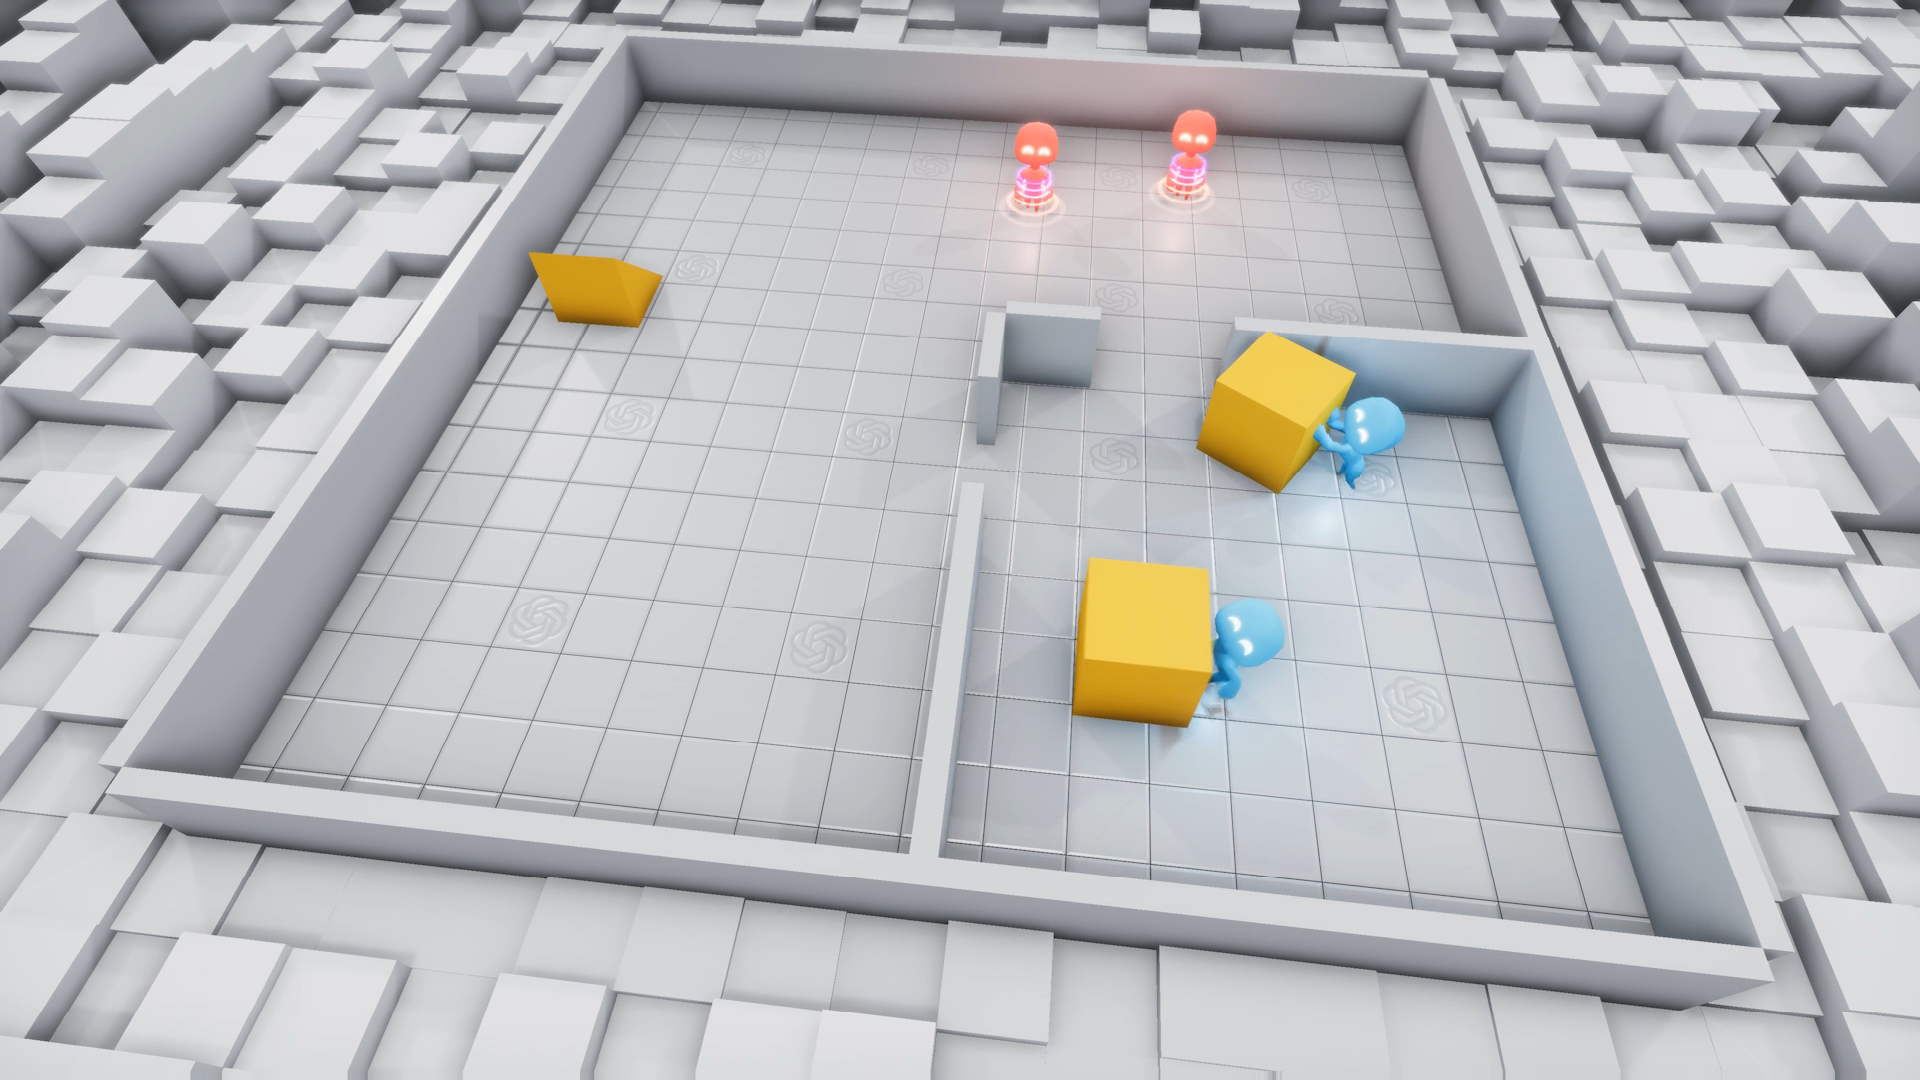
\includegraphics[width=\textwidth]{figures/introduction/hide_and_seek/hide_and_seek_boxes.png}
        \caption{}
        \label{fig:hide_and_seek_boxes}
    \end{subfigure}
    \hfill
    \begin{subfigure}[b]{0.48\textwidth}
        \centering
        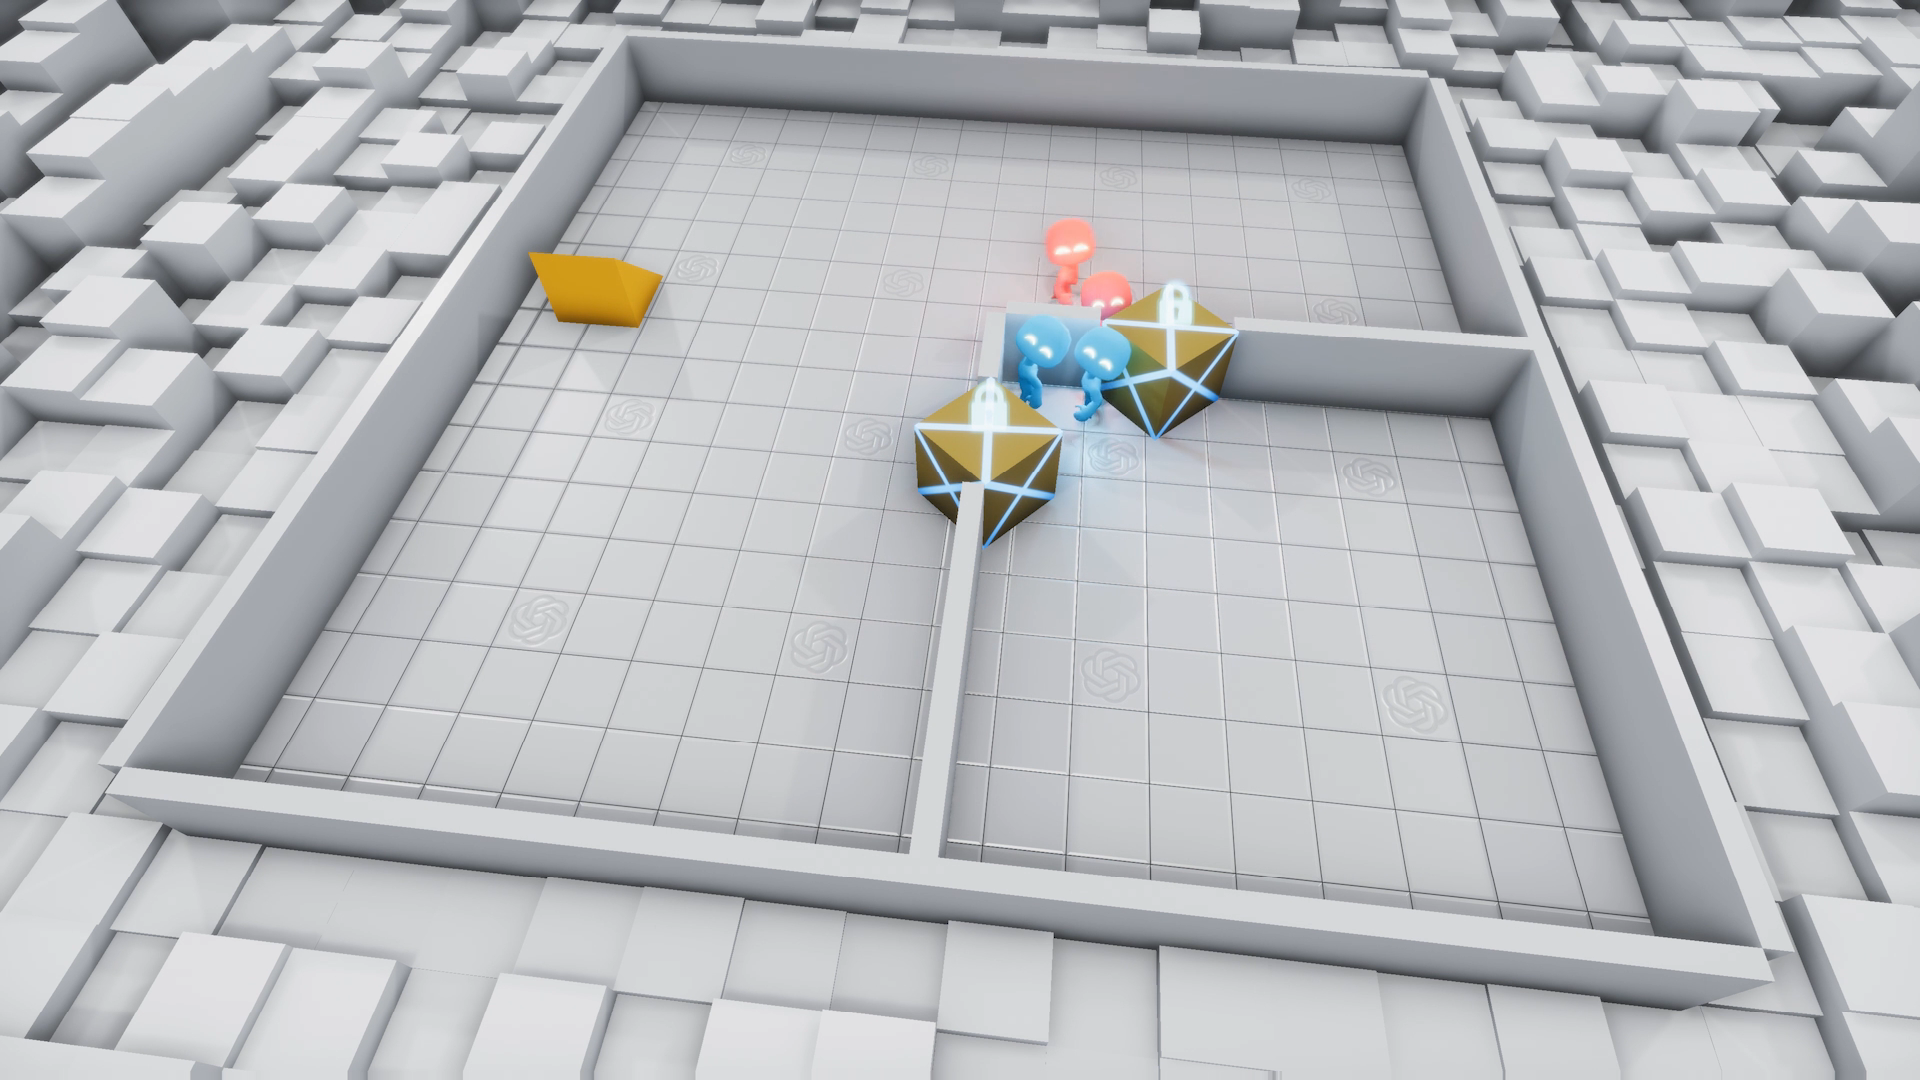
\includegraphics[width=\textwidth]{figures/introduction/hide_and_seek/hide_and_seek_locked.png}
        \caption{}
        \label{fig:hide_and_seek_locked}
    \end{subfigure}

    \vspace{0.5em}

    \begin{subfigure}[b]{0.48\textwidth}
        \centering
        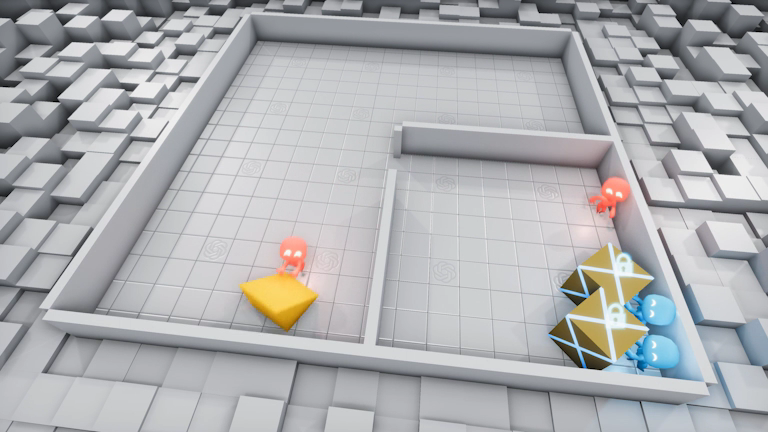
\includegraphics[width=\textwidth]{figures/introduction/hide_and_seek/hide_and_seek_ramp.png}
        \caption{}
        \label{fig:hide_and_seek_ramp}
    \end{subfigure}
    \hfill
    \begin{subfigure}[b]{0.48\textwidth}
        \centering
        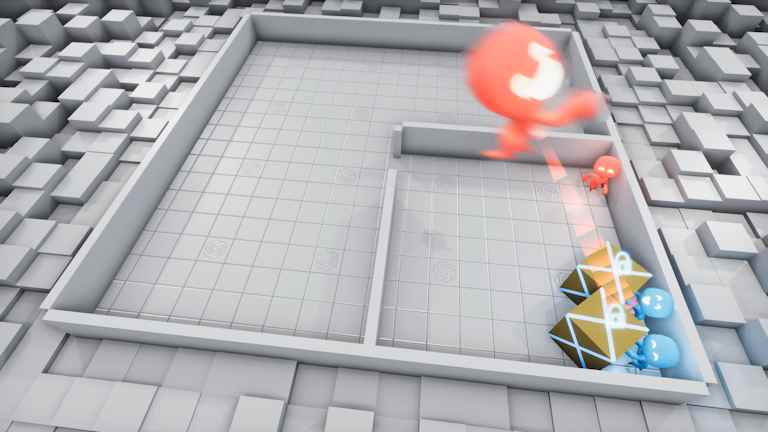
\includegraphics[width=\textwidth]{figures/introduction/hide_and_seek/hide_and_seek_launch.png}
        \caption{}
        \label{fig:hide_and_seek_launch}
    \end{subfigure}
    \caption[Agents playing hide-and-seek.]{Agents playing hide-and-seek \parencite{baker2020emergent}.}
    \label{fig:hide_and_seek}
\end{figure}


In a game environment, such behaviors have limited consequences.
However, agents trained with \gls{rl} are increasingly deployed in open-ended settings where they interact with the real world, notably \glspl{llm} trained with \gls{rl} and deployed as agents.
In such settings, a lack of control can have far more serious consequences.

Such behaviors relate to the problem of alignment (Definition~\ref{def:alignment}), which has become a central concern in \gls{ai} research \parencite{ji2023ai}.
The more capable agents become, the more pressing the need to ensure their alignment.

\begin{definition}{Alignment}{alignment}

Alignment is the problem of ensuring that the behavior of an \gls{ai} system corresponds to the intentions of its designers.

\end{definition}

\subsection{The Black-Box Problem}

The difficulty of ensuring the alignment of such agents stems in part from the fact that we only observe sequences of interactions between the agent and its environment.
These observations reveal how the agent's strategy is realized in particular situations.
However, understanding the strategy itself requires knowing how the agent would behave across all the situations it may encounter.
Since these situations are generally too numerous to be observed exhaustively, a collection of observed behaviors may not be sufficient to characterize the strategy.

To gain further insight into the agent's strategy, an alternative approach is to analyze the agent itself.
However, due to their connectionist nature, \glspl{nn} that model the agent's policy are not directly interpretable.
The information underlying a decision is distributed across many units and connections, making the processes leading to a decision difficult to trace.
\Glspl{nn} are therefore often regarded as \enquote{black-box} models \parencite{guidotti2018survey}.

\subsection{Mechanistic Explainability}

To address this \enquote{black-box} problem, the field of \gls{xai} has emerged \parencite{gunning2019darpa, arrieta2020explainable}.
In the specific context of \gls{rl}, this research area is referred to as \gls{xrl} \parencite{puiutta2020explainable, milani2022explainable}.
\gls{xrl} develops methods for producing explanations that improve our understanding of agent behavior.

These methods can be divided into two general approaches, which are detailed in Section~\ref{subsec:explainable_artificial_intelligence}.
Substitutive explainability adopts the \enquote{black-box} view and seeks to replace the \gls{nn} with alternative models that can be directly understood \parencite{rudin2019stop}.
Intrinsic explainability, in contrast, assumes that \glspl{nn} contain mechanisms that can be explained, the limitation being the lack of adequate tools to analyze them \parencite{olah2020zoom}.
This thesis adopts the intrinsic approach, and more specifically the one that seeks to explain the agent's strategy directly from the internal processes from which it emerges.
We refer to this approach as \gls{me} (Definition~\ref{def:mechanistic_explainability}).\footnote{Commonly referred to as \emph{mechanistic interpretability} \parencite{bereska2024mechanistic}. We use the term \emph{explainability} since the internal mechanisms of an \gls{nn} are not interpretable in the sense of Definition~\ref{def:interpretable}.}

\begin{definition}{Mechanistic Explainability}{mechanistic_explainability}

\gls{me} is the approach that seeks to explain an \gls{nn} by transforming its internal representations into interpretable information.

\end{definition}

\gls{me} is particularly promising because it addresses a core question of \gls{dl}, namely how an \gls{nn} processes information.
Explaining how an agent processes information to make its decisions would therefore improve not only our understanding of agent behavior, but also our understanding of \gls{dl} itself.
Such understanding is also a first step toward control \parencite{mini2023understanding}.

To understand how an \gls{nn} processes information, \gls{me} studies the intermediate representations it learns.
These representations are called \glspl{lr} \parencite{bengio2014representationlearningreviewnew}.
Together, they form the network's \gls{ls}.
Analyzing the structure of this \gls{ls} provides insights into how information relevant to decision-making is organized.
To develop an \gls{xrl} method based on \gls{me}, we need to address several research questions.
\section{Research Questions}
\label{sec:introduction_research_questions}

The first question concerns the analysis of \glspl{lr} themselves.
Numerous methods have been proposed to analyze the \glspl{ls}.
These methods originate from different research communities are rarely compared within a common framework.
This observation leads to our first research question:

\begin{researchquestion}{}{latent_space}
What approaches have been proposed in the literature to analyze the internal workings of \glspl{nn}?
\end{researchquestion}

The second question concerns the organization of existing research in \gls{xrl}.
Several taxonomies have been proposed to organize existing \gls{xrl} methods \parencite{puiutta2020explainable, milani2022explainable}.
However, these taxonomies often rely on approaches initially developed for explainability in supervised settings.
As a result, the organization of existing \gls{xrl} methods remains ambiguous, making it difficult to structure the field.
This observation leads to our second research question:

\begin{researchquestion}{}{taxonomy}
How can existing \gls{xrl} techniques be organized into a taxonomy that accounts for the specificities of \gls{rl}?
\end{researchquestion}

The analysis of existing \gls{xrl} approaches also reveals a third limitation.
Among existing methods for explaining \gls{rl} agents, few adopt a mechanistic perspective.
This observation leads to our third research question:

\begin{researchquestion}{}{mechanisms}
How can the internal representations of \glspl{nn} be exploited to identify the mechanisms underlying the decision-making process of \gls{rl} agents?
\end{researchquestion}

The analysis of existing \gls{xrl} methods highlights a fourth question concerning the evaluation of explanations.
There is no widely accepted set of objective criteria for evaluating the quality and relevance of the explanations produced by these methods.
Existing evaluations often rely on user studies or qualitative analyses, making it difficult to systematically assess the validity of an explanation approach \parencite{doshivelez2017rigorous, milani2022explainable}.
This leads to our fourth research question:

\begin{researchquestion}{}{evaluation}
How can the quality and relevance of explanations produced for \gls{rl} agents be objectively quantified?
\end{researchquestion}

\section{Contributions}
\label{sec:introduction_contributions}

To address these four research questions, this thesis is based on three main contributions.

The first contribution has not yet been published and addresses Research Question~\ref{rq:latent_space}.
In this contribution, we make explicit the working hypothesis that underlies much of the literature on \gls{ls} analysis.
We then organize existing \gls{ls} analysis methods into families to provide an overview of the different approaches.

The second contribution addresses Research Question~\ref{rq:taxonomy}.
This contribution takes the form of a first paper \parencite{alaarabiou:hal-04685607} and an extended English version \parencite{alaarabiou2026taxonomy}, both of which were submitted for review and accepted for publication.
In this contribution, we first clarify what explainability means in \gls{rl} by providing a clear frame of reference.
Building on these frame, we then conduct a comprehensive analysis of the state of the art in \gls{xrl}.

The third contribution addresses Research Questions~\ref{rq:mechanisms} and~\ref{rq:evaluation}.
In \textcite{alaarabiou2026car}, which has been reviewed and accepted for publication, we introduce \gls{car}, an \gls{xrl} method based on the principles of \gls{me}.
By analyzing the \glspl{lr}, \gls{car} produces explanations in the form of clusters of states that are similar from the agent's own perspective.
We further show that independently trained networks develop similarly structured representations, indicating that these representations reflect properties of the task rather than of a particular network.

This thesis can be viewed as a synthesis of these three contributions.

\section{Thesis Structure}
\label{sec:introduction_thesis_structure}

\begin{figure}[t]
    \centering
    \resizebox{\textwidth}{!}{
        \begin{tikzpicture}[
            chapter/.style={rectangle, draw, rounded corners, minimum height=1.6cm,
                            minimum width=2.9cm, align=center, font=\small, text width=2.7cm},
            legend/.style={rectangle, draw, rounded corners, font=\small,
                           inner xsep=8pt, inner ysep=5pt},
            >={Stealth},
            % Each category has its own color AND its own border style, so the
            % figure stays readable in grayscale: dashed for technical
            % background, solid for surveys, double line for the method.
            background/.style={draw=myblue,  fill=myblue!12, dashed, line width=1pt},
            survey/.style={draw=mygreen, fill=mygreen!12},
            method/.style={draw=myred,   fill=myred!12, double=myred!12,
                           double distance=1.6pt},
        ]

        % Chapter number (small, on top) followed by the chapter name in bold.
        \newcommand{\chapterbox}[2]{{\footnotesize Chapter~\ref{#1}}\\[3pt]\textbf{#2}}

        % Two parallel tracks, deep learning (top) and reinforcement learning
        % (bottom), which converge on the method chapter.
        \node[chapter, background]  (dl)   at (0, 1.1)   {\chapterbox{chap:deep_learning}{Deep\\Learning}};
        \node[chapter, survey] (ls)   at (3.5, 1.1) {\chapterbox{chap:latent_space_analysis}{Latent\\Space}};
        \node[chapter, background]  (rl)   at (0, -1.1)  {\chapterbox{chap:reinforcement_learning}{Reinforcement\\Learning}};
        \node[chapter, survey] (xrl)  at (3.5, -1.1){\chapterbox{chap:explainability_in_reinforcement_learning}{Explainability\\in \gls{rl}}};
        \node[chapter, method]   (car)  at (7.5, 0)   {\chapterbox{chap:clustering_agent_representations}{\gls{car}\\Method}};
        \node[chapter, method]   (exp)  at (11, 0)    {\chapterbox{chap:experiments}{Experiments}};

        % Within each track.
        \draw[->, thick] (dl)  -- (ls);
        \draw[->, thick] (rl)  -- (xrl);

        % Both tracks converge on the method chapter.
        \draw[->, thick] (ls.east)  -- ++(0.55, 0) |- ([yshift=0.35cm]car.west);
        \draw[->, thick] (xrl.east) -- ++(0.55, 0) |- ([yshift=-0.35cm]car.west);

        \draw[->, thick] (car) -- (exp);

        \matrix[ampersand replacement=\&, column sep=0.8cm, inner sep=0pt] at (5.5, -2.8) {
            \node[legend, background]  {Technical background}; \&
            \node[legend, survey] {Survey}; \&
            \node[legend, method]   {Method}; \\
        };

        \end{tikzpicture}
    }
    \caption{Structure of the thesis.}
    \label{fig:thesis_map}
\end{figure}


The thesis is organized into a sequence of chapters, with each chapter falling into one of these three categories:
\begin{itemize}
\item[] \textcolor{myblue}{\textbf{Technical background}} chapters introduce fundamental concepts required to understand the subsequent contributions.
\item[] \textcolor{mygreen}{\textbf{Survey}} chapters review the existing literature around a specific research question.
The organization adopted in each of these surveys is original and therefore constitutes a contribution of this thesis.
\item[] \textcolor{myred}{\textbf{Method}} chapters present \gls{car}, our \gls{me} method for \gls{rl}.
\end{itemize}

Following these categories, the chapters are organized as shown in Figure~\ref{fig:thesis_map} and detailed below:
\begin{description}[style=nextline, leftmargin=1.5em, itemsep=0.5em]
\item[\textcolor{myblue}{\textbf{Deep Learning (Chapter~\ref{chap:deep_learning}, technical background)}}]
This chapter introduces the fundamental concepts of \gls{dl}, the training paradigm used to optimize deep \glspl{nn}.
It begins with an overview of the historical developments that led to the emergence of the field.
It then formalizes the objective of \gls{dl} and describes the structure of artificial \glspl{nn}.
Next, it explains how the learning process shapes these networks and how the resulting models are evaluated.
It concludes by showing that \glspl{nn} progressively transform their inputs into intermediate representations, whose study motivates the following chapter.

\item[\textcolor{mygreen}{\textbf{Latent Space Analysis (Chapter~\ref{chap:latent_space_analysis}, survey)}}]
This chapter addresses Research Question~\ref{rq:latent_space} by providing a survey of existing approaches for analyzing the \glspl{ls}.
It first makes explicit the working hypothesis that underlies much of this literature, which we refer to as the \ConceptHypothesisName.
It then reviews four families of methods, based respectively on probing, interpretable directions, feature superposition, and clustering.
These families are compared within a common synthesis, which highlights their shared goal of understanding how information is organized in \glspl{lr}.
The chapter closes by discussing the absence of consensus on how to evaluate whether these methods truly capture the concepts of a model.

\item[\textcolor{myblue}{\textbf{Reinforcement Learning (Chapter~\ref{chap:reinforcement_learning}, technical background)}}]
This chapter introduces the fundamental concepts of \gls{rl}.
It begins with an overview of the milestones that led to the emergence of \gls{rl} as a unified field.
It then clarifies what is meant by an agent and formalizes the problem that \gls{rl} algorithms aim to solve.
Next, it explains how a policy is progressively refined through interaction with the environment to approach the optimal policy.
It concludes by showing how the combination of \gls{rl} and \gls{dl} gives rise to agents that are both powerful and difficult to understand.

\item[\textcolor{mygreen}{\textbf{Explainability in Reinforcement Learning (Chapter~\ref{chap:explainability_in_reinforcement_learning}, survey)}}]
This chapter addresses Research Question~\ref{rq:taxonomy} by reviewing existing approaches to explainability in \gls{rl}.
It first clarifies what is meant by an explanation in the context of \gls{xai}.
It then presents a taxonomy that categorizes \gls{xrl} methods according to the subject of the explanation, the source of information and the form it takes.
This taxonomy is used to structure a state-of-the-art.
The chapter concludes with three observations from this review: the absence of explanations of the learning process, a lack of unified evaluation metrics, and few intrinsic methods for explaining the deep neural policies.

\item[\textcolor{myred}{\textbf{The CAR Method (Chapter~\ref{chap:clustering_agent_representations}, method)}}]
This chapter addresses Research Questions~\ref{rq:mechanisms} and~\ref{rq:evaluation} by proposing \gls{car}, a new method for explainability in \gls{rl} based on the analysis of \glspl{lr}.
It first lays out the theoretical assumption underlying the method, which we term the \RepresentationConvergenceHypothesisName.
It then details the method itself, which extracts \glspl{lr} from surrogate policies and automatically detects \glspl{cs} through clustering.
Next, it introduces the \gls{cu}, \gls{as}, and \gls{acu} metrics, which evaluate the consistency and the abstraction of the resulting clusters without manual intervention.
Finally, it situates \gls{car} within the broader landscape of \gls{me}.

\item[\textcolor{myred}{\textbf{Evaluation of the CAR Method (Chapter~\ref{chap:experiments}, method)}}]
This chapter presents the implementation and experimental evaluation of the proposed method.
It first describes the software implementation of the \gls{car} pipeline and the experimental configuration, based on six environments from the Atari benchmark.
It then evaluates how faithfully the surrogate policies reproduce the behavior of the initial policy.
Next, a quantitative analysis measures the consistency and the abstraction of the clusters across the layers of the network.
Finally, a qualitative analysis examines the semantic content of the clusters, which capture aspects such as episode progression, specific game situations, and behavioral patterns.

\item[\textbf{Conclusion (Chapter~\ref{chap:conclusion})}]
This chapter closes the thesis by revisiting each research question in light of the contributions presented.
It then discusses the limitations of these contributions.
These limitations open several directions for future research, which are presented next.
Finally, the chapter ends with a broader reflection on this work.
\end{description}

The mathematical notation used throughout this thesis is summarized on page~\pageref{chap:notation}, and the acronyms are listed on page~\pageref{chap:acronyms}.

Finally, in the interest of transparency, we specify how generative \gls{ai} tools were used in this work.
\Glspl{llm} served as assistants during the preparation of this thesis.
They were used for writing tasks, including translation, wording improvement, and proofreading.
They were also used for software development, including code implementation and review.
Finally, they were used to support scientific work, including the identification of relevant documents and discussion of approaches.
They were not used as autonomous scientific sources.
All generated outputs were systematically reviewed, and the author takes full responsibility for the content presented in this thesis.

Now that the research context and objectives have been presented, we can turn to the first chapter, which introduces the fundamentals of \gls{dl}.

\chapter{Deep Learning}
\label{chap:deep_learning}

\glsresetall

This chapter introduces the fundamental concepts of \gls{dl}, the training paradigm used to optimize deep \glspl{nn}.
The objective is to provide the necessary foundation in \gls{dl} for the ideas developed throughout the rest of this thesis.
Its structure is as follows:

\begin{itemize}
    \item[]Section~\ref{sec:deep_learning_historical_developments}: An overview of the historical developments that led to the emergence of the field.
    \item[]Section~\ref{sec:deep_learning_objective}: A formalization of the objective underlying \gls{dl} algorithms.
    \item[]Section~\ref{sec:deep_learning_neural_network_structure}: An examination of the structure of artificial \glspl{nn}.
    \item[]Section~\ref{sec:deep_learning_learning}: An explanation of how the learning process shapes \glspl{nn}.
    \item[]Section~\ref{sec:deep_learning_evaluation}: A discussion of how such models are evaluated.
    \item[]Section~\ref{sec:deep_learning_conclusion}: A summary of the concepts introduced in the chapter and a discussion of the theoretical limitations of \gls{dl}.
\end{itemize}

\section{Historical Developments}\label{sec:historical_developments}

\begin{figure}[t]
    \centering
    \resizebox{0.85\textwidth}{!}{
        \Timeline[1943,2025,0.3]{
            \event{1943}{mcculloch1943logical}{Mathematical model of \textbf{Neural Networks}.}{5.5cm}{1cm}{0.05cm}{\small}{blue!10}
            \event{1958}{rosenblatt1958perceptron}{\textbf{Perceptron}, the first trainable connectionist learning algorithm.}{5.5cm}{1cm}{-0.05cm}{\small}{cyan!10}
            \event{1986}{rumelhart1986learning}{\textbf{Multi-Layer Backpropagation}, enabling the training of neural networks.}{6cm}{1cm}{-0.05cm}{\small}{red!10}
            \event{1989}{lecun1989backpropagation}{Introduction of \textbf{Convolutional Neural Networks}, for processing image inputs.}{6cm}{1cm}{0.05cm}{\small}{purple!10}
            \event{1997}{hochreiter1997long}{\textbf{Long Short-Term Memory}, enabling neural networks to model temporal dependencies.}{6cm}{1cm}{0.125cm}{\small}{green!10}
            \event{2009}{raina2009large}{\textbf{GPU Acceleration} for large-scale neural network training.}{5.5cm}{1cm}{-0.05cm}{\small}{orange!10}
            \event{2016}{goodfellow2016deep}{Publication of the reference \textbf{Deep Learning Book}.}{5.5cm}{1cm}{0.05cm}{\small}{yellow!15}
            \event{2017}{vaswani2017attention}{\textbf{Transformer Architecture}, enabling efficient processing of long and variable-length sequences.}{5.5cm}{1cm}{-0.125cm}{\small}{cyan!10}
        }
    }
    \caption{Evolution of deep learning.}
    \label{fig:evolution_deep_learning}
\end{figure}

\glspl{nn} and \gls{dl} emerged from an ambition to study the expressive capabilities of organic brain.
The first major milestone came in 1943 with the proposal of a mathematical model of an artificial neuron, with a formulation of networked interactions \cite{mcculloch1943logical}.
This work established the key idea that networks of simple units can give rise to complex computations.
The focus was on representational power, not on the ability of such systems to learn.
As a result, this work remained largely theoretical and had limited practical applications.

A major step toward operationalizing the idea of \glspl{nn} was achieved with the perceptron algorithm in 1958 \cite{rosenblatt1958perceptron}.
It was designed to adjust its parameters from input–output pairs in order to approximate a target function.
The perceptron fundamental limitations were exposed in 1969, showing that it could not learn functions as simple as the exclusive-or \cite{minsky1969introduction}.
At the same time, it was demonstrated that stacking multiple perceptrons could, in principle, represent such functions.
However, no effective training procedure for these multi-layer architectures was available at the time. It was only in 1986 that researchers introduced gradient descent as an effective method for training deep \glspl{nn} \cite{rumelhart1986learning}.
From this point onward, the emergence of \gls{dl} is retrospectively situated, even though the term itself appeared later.
\gls{dl} is defined as the training of deep \glspl{nn} using gradient-based optimization methods.

It took several decades before \gls{dl} reached the level of prominence it has today.
One major obstacle was the absence of theoretical guarantees regarding the convergence of learning algorithms.
Although the universal approximation theorem shows that \glspl{nn} can represent a wide class of functions \cite{hornik1989multilayer}, it did not ensure that such representations could be effectively learned through optimization methods like gradient descent.
This lack of rigorous guarantees initially reduced interest within the academic community.
As a result, early progress relied largely on empirical breakthroughs.

These empirical advances were made possible by two key developments: the availability of large-scale datasets and significant improvements in computational infrastructure.
\gls{dl} methods require vast amounts of data to perform well, and the rise of the internet alongside the digitization of information enabled the creation of such datasets \cite{hilbert2011world}.
The use of graphics processing units for large-scale training, demonstrated in 2009, greatly increased computational capacity and made it feasible to train large-scale models \cite{raina2009large, krizhevsky2012imagenet}.

At the same time, researchers developed architectures specifically designed for different types of data, allowing \gls{dl} to address an increasingly wide range of problems.
\glspl{cnn} were introduced in 1989 to process images, using local, weight-shared filters that exploit the spatial structure of pixel grids \cite{lecun1989backpropagation}.
\gls{lstm} networks were later proposed in 1997 to process temporal sequences, introducing gating mechanisms able to retain relevant information over long time horizons \cite{hochreiter1997long}.
More recently, the Transformer architecture, relying entirely on the attention mechanism, was introduced in 2017 to process long, variable-length sequences of strongly interconnected elements, allowing every element to attend directly to every other element regardless of their distance within the sequence \cite{vaswani2017attention}.
This growing body of knowledge was consolidated in 2016 in a reference textbook that formalized \gls{dl} as a coherent field of study \cite{goodfellow2016deep}.

These changes paved the way for the rise of \gls{dl} as it is known today.
\gls{dl} has achieved remarkable success across a wide range of domains, including computer vision \cite{krizhevsky2012imagenet}, complex games \cite{silver2017mastering}, content recommendation \cite{covington2016deep}, bio-chemistry \cite{jumper2021highly}, as well as the now essential digital assistants based on \glspl{llm} \cite{brown2020language}.
The diversity of these applications explains the enthusiasm for this technology, which continues to redefine the boundaries of what was once considered automatable.

Figure~\ref{fig:evolution_deep_learning} provides a timeline of the key milestones that shaped deep learning.
\section{Objective}\label{sec:deep_learning_objective}

Now that the main developments that led to the rise of \gls{dl} have been outlined, it is necessary to formalize what is actually being achieved when performing \gls{dl}.
To ensure clarity, the supervised learning setting will be considered, specifically applied to a regression task.
This framework serves as a standard reference in the field, as all building blocks of \gls{dl} applications are built upon this fundamental formalism.

In this setting, learning consists of progressively shaping a \gls{nn} that serves as an approximation of a target function.
At initialization, the network does not yet provide a meaningful representation of this function.
Since a \gls{nn} is a parametric function, its parameters are updated during training to better approximate the target function.
It gradually becomes capable of capturing the relationship between inputs and outputs through successive parameter updates during training.
For this reason, \gls{dl} is naturally situated within the framework of machine learning.
A standard definition of machine learning is:
\begin{displayquote}
\textit{A computer program is said to learn from experience $E$ with respect to some class of tasks $T$ and performance measure $P$, if its performance at tasks in $T$, as measured by $P$, improves with experience $E$.} \parencite{mitchell1997machine}
\end{displayquote}

When this formulation is adapted to \gls{dl}, the following correspondences hold:
\begin{itemize}
\item The computer program corresponds to the learning algorithm, which is responsible for adjusting the network's parameters.
\item The task $T$ consists of learning a \gls{nn} that provides a good approximation of the target function.
\item The performance measure $P$ corresponds to a function used to evaluate the quality of this approximation.
\item The experience $E$ takes the form of a dataset composed of input--output pairs derived from the function to be approximated.
\end{itemize}

The function to be approximated is denoted by $f$.
As with any function, it defines a mapping from an input to an output: $\vect{x} \in \mathcal{X}$ denotes an input and $\vect{y} \in \mathcal{Y}$ the corresponding output.
The function $f$ is therefore characterized by an input space $\mathcal{X}$ and an output space $\mathcal{Y}$, and can be formally written as $f : \mathcal{X} \to \mathcal{Y}$.
For simplicity of exposition, both $\mathcal{X}$ and $\mathcal{Y}$ are assumed to be vector spaces throughout this thesis.
This assumption is adopted solely to facilitate the presentation, as the framework can be readily extended to more general settings.
The notation $\hat{\cdot}$ indicates that a given object is an approximation of another.
Since the goal of the trained \gls{nn} is to approximate $f$, this approximation is denoted by $\hat{f} : \mathcal{X} \to \mathcal{Y}$.
Given an input $\vect{x} \in \mathcal{X}$, the output of the approximating function $\hat{f}(\vect{x})$ is denoted by $\hat{\vect{y}}$.

It is important to emphasize that the target function $f$ is generally not known explicitly.
If it were, there would be no need to learn an approximation, since the true function would already provide the exact mapping.
In practice, only a finite set of observations generated by $f$ is available, organized in what is called a dataset.
To distinguish between the different samples, an index $i$ is introduced, allowing input--output pairs of the form $(\vect{x}^{(i)}, \vect{y}^{(i)})$ to be defined.
This leads to the following formulation for a dataset $\mathcal{D}$ of size $N$, where $N$ denotes the number of available examples:
\begin{equation}
    \mathcal{D} = \{(\vect{x}^{(i)}, \vect{y}^{(i)})\}_{i=1}^{N}.
    \label{eq:dataset}
\end{equation}

Now that the representation of the target function $f$ has been established, the next question is what makes a function $\hat{f}$ a good approximation of it.
For a given input $\vect{x}^{(i)}$, this means that the \gls{nn} output $\hat{\vect{y}}^{(i)}$ should be close to the true output $\vect{y}^{(i)}$.
To quantify the quality of this approximation, a function $\mathcal{L}$ is introduced that measures the discrepancy between predictions and target values.
This function called the loss function plays a central role as it guides the learning process.
In regression settings, a common choice is the \gls{mse}, defined as:
\begin{equation}
    \mathcal{L}(\hat{\vect{y}}, \vect{y}) = \|\hat{\vect{y}} - \vect{y}\|_2^2.
    \label{eq:mse}
\end{equation}
Thanks to this loss, it is now possible to rigorously define the performance measure $P$.
This performance measure corresponds to the average loss over the dataset and can therefore be written as:
\begin{equation}
    P = \frac{1}{N} \sum_{i=1}^{N} \mathcal{L}(\hat{f}(\vect{x}^{(i)}), \vect{y}^{(i)}).
    \label{eq:performance_measure}
\end{equation}

This formulation captures the mathematical core of the learning objective, namely finding a \gls{nn} $\hat{f}$ that minimizes the prediction error over the dataset $\mathcal{D}$.
Since the target function $f$ may take many different forms, $\hat{f}$ must be expressive enough to approximate a broad range of such functions.
\gls{nn} architectures are well suited to this requirement, as they can represent a wide range of functional mappings, whose composition is detailed in the following section.
\section{Neural Network Structure}\label{sec:deep_learning_neural_network_structure}

\glspl{nn} are called connectionist models.
Rather than modeling information processing through a set of explicit rules, they rely on a flow of signals distributed within a computational structure.
Their architecture is composed of a large number of simple computational units, which operate on partial representations and exchange signals across the network.
A complex pattern of weighted connections between these units enables the transformation and propagation of information.

To simplify the presentation, the focus is placed on the \gls{mlp} architecture.
Although more specialized architectures exist, which are presented in Section~\ref{sec:deep_learning_specialized_architectures}, the \gls{mlp} forms a fundamental building block of \gls{dl}.
All the essential mechanisms are present in it, making it a particularly suitable framework for introducing key concepts.

This section therefore begins by examining the artificial neuron, the fundamental computational unit underlying the \gls{mlp}.
It then explains how these neurons are organized into layers.
Finally, it concludes with a general description of the \gls{nn} as a whole.

\subsection{Neurons}

The artificial neuron is the basic building block of \glspl{nn}.
It is through these units that all computations within the network are carried out.
A neuron receives a set of input signals from other neurons, where these inputs are represented as real-valued numbers.
It produces an output, also a real-valued number, which is transmitted to subsequent neural units.
Its internal state, called the activation, reflects its level of response and encodes the information processed for a given input.
This activation, or lack thereof, is then used as input information by other neurons to determine their own activations, thereby propagating information through the network.

A neuron is characterized by:
\begin{itemize}
\item a set of incoming connections from other neurons,
\item a weight associated with each of these connections,
\item a bias term,
\item a differentiable nonlinear activation function,
\item a scalar activation state.
\end{itemize}

The activation of a neuron is determined by a weighted combination of its input signals, to which a bias is added, followed by the application of a nonlinear activation function.
Mathematically, for a neuron receiving inputs $(x_1, \dots, x_n)$, its activation $h$ is given by:
\begin{equation}
h = \sigma\left(\sum_{i=1}^{n} w_i x_i + b\right),
\label{eq:neuron_activation}
\end{equation}
where:
\begin{itemize}
\item $w_i$ is the weight associated with the $i$-th incoming connection,
\item $b$ is the bias,
\item $\sigma$ is the activation function.
\end{itemize}

Figure~\ref{fig:artificial_neuron} shows a schematic view of this basic unit.
The set of weights $w_1, \dots, w_i$ with the bias $b$ constitute the parameters of the neuron, and they are the elements that evolve during training.
The magnitude of a weight $w$, relative to the others, indicates how strongly a neuron depends on the activation of the neurons to which it is connected.
A large positive weight means that a high activation in the connected neuron tends to increase the activation of the receiving neuron, whereas a negative weight implies the opposite effect.
In this way, the weights modulate the strength and nature of the connections between neurons, thereby defining the overall pattern of interaction within the network.

\begin{figure}[t]
    \centering
    \resizebox{0.85\textwidth}{!}{
        \begin{tikzpicture}[
            >={Stealth},
            neuron/.style={circle, draw, minimum size=1.2cm, inner sep=0pt},
            function/.style={rectangle, draw, minimum width=3.4cm, minimum height=3.4cm,
                            align=center, text width=3cm, inner sep=2pt},
            dotted line/.style={dotted, line width=2pt},
        ]

        % Background circle
        \draw (0,0) circle (5);

        % Combination function (left)
        \node[function] (combination_function) at (-2.2, 0) {
            Combination function \\[4pt] $\sum_{i=1}^{n} w_i x_i + b$
        };

        % Activation function (right)
        \node[function] (activation_function) at (2.2, 0) {
            Activation function \\[4pt] $\sigma(\cdot)$
        };

        % Arrow between the two functions
        \draw[->] (combination_function.east) -- (activation_function.west);

        % Bias (constant 1) and its connection
        \node[neuron] (bias) at (-2.2, -3.5) {$1$};
        \draw[->] (bias) -- (combination_function) node[midway, right] {$b$};

        % Incoming neurons – unrolled for clarity and to avoid parsing errors
        \node[neuron] (in0) at (-8, 5) {$x_1$};
        \draw[->] (in0) -- (combination_function) node[midway, above] {$w_1$};

        \node[neuron] (in1) at (-8, 3) {$x_2$};
        \draw[->] (in1) -- (combination_function) node[midway, above] {$w_2$};

        \node[neuron] (in2) at (-8, -3) {$x_{n-1}$};
        \draw[->] (in2) -- (combination_function) node[midway, above] {$w_{n-1}$};

        \node[neuron] (in3) at (-8, -5) {$x_n$};
        \draw[->] (in3) -- (combination_function) node[midway, above] {$w_n$};

        % Dotted line indicating more neurons
        \draw[dotted, thick] (-8, -1.1) -- (-8, 1.1);

        % Output activation node
        \node[align=center] (activation_output) at (7,0) {Activation \\ $h$};
        \draw[->] (activation_function.east) -- (activation_output.west);

        \end{tikzpicture}
    }
    \caption{Artificial neuron.}
    \label{fig:artificial_neuron}
\end{figure}

The activation function $\sigma$ models how a neuron transforms incoming signals into its output activation.
Originally, this function was inspired by biological neurons, with the goal of mimicking the firing behavior of organic cells.
However, modern \gls{dl} no longer relies on this biological interpretation.
In practice, any function that is nonlinear, differentiable, and computationally efficient can be used.
Nonlinearity is a crucial property, since without it a \gls{nn} would reduce to a composition of linear transformations, and would therefore be unable to approximate complex functions.

\subsection{Layers}

In \gls{mlp} architectures, neurons are organized into successive layers, as illustrated in Figure~\ref{fig:general_architecture_multilayer_perceptron}.
This layered structure determines how neurons are connected.
In this setting, each neuron receives inputs from all neurons in the preceding layer and sends its output to all neurons in the following layer.
As a result, neurons within the same layer do not interact with each other.

\begin{figure}[t]
    \centering
    \resizebox{\textwidth}{!}{
        \begin{tikzpicture}[
            x=0.52cm, y=0.52cm,
            neuron/.style={circle, draw, minimum size=9pt, inner sep=0pt},
            arr/.style={-{Stealth[length=3pt, width=2.5pt]}},
        ]

        %% ── Layers ─────────────────────────────────────────────────────────────────
        \foreach \lx/\idx in {-9/1, -5/2, -2/3, 2/4, 5/5, 9/6}{
        \foreach \ly/\jdx in {4/1, 2/2, -2/3, -4/4}{
            \node[neuron] (L\idx N\jdx) at (\lx,\ly) {};
        }
        \draw[dotted, thick] (\lx, 0.75) -- (\lx, -0.75);
        }

        %% Layer labels (1 unit above top neuron)
        \node[font=\scriptsize] at (-9,  5.2) {Layer $0$};
        \node[font=\scriptsize] at (-5,  5.2) {Layer $1$};
        \node[font=\scriptsize] at (-2,  5.2) {Layer $l{-}1$};
        \node[font=\scriptsize] at ( 2,  5.2) {Layer $l$};
        \node[font=\scriptsize] at ( 5,  5.2) {Layer $L{-}1$};
        \node[font=\scriptsize] at ( 9,  5.2) {Layer $L$};

        %% ── Fully-connected pairs ───────────────────────────────────────────────────
        \foreach \i in {1,...,4}{
        \foreach \j in {1,...,4}{
            \draw[arr] (L1N\i) -- (L2N\j);
            \draw[arr] (L3N\i) -- (L4N\j);
            \draw[arr] (L5N\i) -- (L6N\j);
        }
        }

        %% ── Horizontal dots between layer groups ────────────────────────────────────
        \draw[dotted, thick] (-4, 0) -- (-3, 0);
        \draw[dotted, thick] ( 3, 0) -- ( 4, 0);

        %% ── Input vector ────────────────────────────────────────────────────────────
        \node (iv0) at (-12.5,  2.4) {$x_1$};
        \node (iv1) at (-12.5,  1.2) {$x_2$};
        \node (iv2) at (-12.5,  0.0) {$\vdots$};
        \node (iv3) at (-12.5, -1.2) {$x_{n_0-1}$};
        \node (iv4) at (-12.5, -2.4) {$x_{n_0}$};

        \draw (-13.25, 2.8) -- (-13.5, 2.8) -- (-13.5,-2.8) -- (-13.25,-2.8);
        \draw (-11.75, 2.8) -- (-11.5, 2.8) -- (-11.5,-2.8) -- (-11.75,-2.8);

        \node[align=center, font=\scriptsize] at (-12.5, 4.3)
        {Input\\vector $\vect{x}$};

        \draw[arr] (iv0.east) -- (L1N1);
        \draw[arr] (iv1.east) -- (L1N2);
        \draw[arr] (iv3.east) -- (L1N3);
        \draw[arr] (iv4.east) -- (L1N4);

        %% ── Output vector ───────────────────────────────────────────────────────────
        \node (ov0) at (12.5,  2.4) {$\hat{y}_1$};
        \node (ov1) at (12.5,  1.2) {$\hat{y}_2$};
        \node (ov2) at (12.5,  0.0) {$\vdots$};
        \node (ov3) at (12.5, -1.2) {$\hat{y}_{n_L-1}$};
        \node (ov4) at (12.5, -2.4) {$\hat{y}_{n_L}$};

        \draw (11.75, 2.8) -- (11.5, 2.8) -- (11.5,-2.8) -- (11.75,-2.8);
        \draw (13.25, 2.8) -- (13.5, 2.8) -- (13.5,-2.8) -- (13.25,-2.8);

        \node[align=center, font=\scriptsize] at (12.5, 4.3)
        {Model's\\prediction $\hat{\vect{y}}$};

        \draw[arr] (L6N1) -- (ov0.west);
        \draw[arr] (L6N2) -- (ov1.west);
        \draw[arr] (L6N3) -- (ov3.west);
        \draw[arr] (L6N4) -- (ov4.west);

        %% ── Bottom braces ───────────────────────────────────────────────────────────

        % Input layer brace
        \draw[decorate, decoration={brace, amplitude=4pt, mirror}]
            (-9.8, -5.2) -- (-8.2, -5.2)
            node[midway, below=6pt, font=\scriptsize, align=center]
            {Input\\layer};

        % Hidden layers brace
        \draw[decorate, decoration={brace, amplitude=4pt, mirror}]
            (-5.8, -5.2) -- (5.8, -5.2)
            node[midway, below=6pt, font=\scriptsize, align=center]
            {Hidden layers};

        % Output layer brace
        \draw[decorate, decoration={brace, amplitude=4pt, mirror}]
            (8.2, -5.2) -- (9.8, -5.2)
            node[midway, below=6pt, font=\scriptsize, align=center]
            {Output\\layer};

        \end{tikzpicture}
    }
    \caption{Multilayer Perceptron Architecture.}
    \label{fig:general_architecture_multilayer_perceptron}
\end{figure}

Three types of layers are distinguished:
\begin{itemize}
\item an \emph{input layer}, which directly receives input,
\item one or more \emph{hidden layers} (also referred to as intermediate layers), which perform intermediate transformations,
\item an \emph{output layer}, which produces the final prediction.
\end{itemize}

The input and output layers play a specific role.
The input layer has no preceding layer, as its neurons directly encode the components of the input vector $\vect{x}$.
Conversely, the output layer has no subsequent layer, and its neurons produce the model's prediction $\hat{\vect{y}}$.
This structure imposes a direct correspondence between the dimensionality of the input space and the number of neurons in the input layer, and similarly between the output space and the number of neurons in the output layer.

When describing \glspl{nn}, it is more common to reason at the level of layers rather than individual neurons.
This perspective allows interactions between layers to be modeled in a matrix form.
Such a representation enables efficient parallel computation and forms the basis of modern \gls{dl} implementations \parencite{krizhevsky2012imagenet}.

Within this framework, it is useful to introduce the notion of layer activations.
The activation of a layer corresponds to the activations of all its neurons, organized into a vector.
For a layer $l$ composed of $n_l$ neurons, the activations are given by:
\begin{equation}
\latentRepresentation[l] = [h_1^{(l)}, \dots, h_{n_l}^{(l)}].
\label{eq:layer_activation_vector}
\end{equation}
Using this formulation, the interaction between two consecutive layers can be written compactly as:
\begin{equation}
\latentRepresentation[l] = \sigma^{(l)}\left(\mat{W}^{(l)} \latentRepresentation[l-1] + \vect{b}^{(l)}\right),
\label{eq:layer_interaction}
\end{equation}
where:
\begin{itemize}
\item $\latentRepresentation[l-1]$ represents the activations vector of the previous layer,
\item $\mat{W}^{(l)} \in \mathbb{R}^{n_l \times n_{l-1}}$ is the weight matrix connecting layer $l-1$ to layer $l$,
\item $\vect{b}^{(l)} \in \mathbb{R}^{n_l}$ is the bias vector associated with layer $l$,
\item $\sigma^{(l)}$ is the activation function applied element-wise to the neurons of layer $l$.
\end{itemize}

This matrix-vector representation is visualized in Figure~\ref{fig:matrix_interaction_between_layers}, which highlights how each neuron in layer $l$ receives weighted signals from all neurons in the previous layer.

\newcommand{\layerLeftX}{-9}
\newcommand{\layerRightX}{9}
\newcommand{\contentY}{-8.5}
\pgfmathsetmacro{\centerX}{(\layerLeftX + \layerRightX)/2}

\begin{figure}[t]
    \centering
    \resizebox{0.9\textwidth}{!}{
        \begin{tikzpicture}[
            x=0.65cm, y=0.8cm,
            neuron/.style={circle, draw, minimum size=40pt, inner sep=1pt},
            arr/.style={-{Stealth[length=4pt, width=3pt]}},
        ]

        %%── Previous layer  (x = \layerLeftX) ───────────────────────────────────────
        \node[neuron] (P1) at (\layerLeftX,  3.5) {$h^{(l-1)}_1$};
        \node[neuron] (P2) at (\layerLeftX,  1.5) {$h^{(l-1)}_2$};
        \node[neuron] (P3) at (\layerLeftX, -1.5) {$h^{(l-1)}_{n_{l-1}-1}$};
        \node[neuron] (P4) at (\layerLeftX, -3.5) {$h^{(l-1)}_{n_{l-1}}$};

        \draw[dotted, thick] (\layerLeftX, 0.5) -- (\layerLeftX, -0.5);
        \node[font=\large] at (\layerLeftX, 5.2) {Layer $l-1$};

        %%── Current layer  (x = \layerRightX) ───────────────────────────────────────
        \node[neuron] (C1) at (\layerRightX,  3.5) {$h^{(l)}_1$};
        \node[neuron] (C2) at (\layerRightX,  1.5) {$h^{(l)}_2$};
        \node[neuron] (C3) at (\layerRightX, -1.5) {$h^{(l)}_{n_l-1}$};
        \node[neuron] (C4) at (\layerRightX, -3.5) {$h^{(l)}_{n_l}$};

        \draw[dotted, thick] (\layerRightX, 0.5) -- (\layerRightX, -0.5);
        \node[font=\large] at (\layerRightX, 5.2) {Layer $l$};

        %%── Fully-connected arrows ──────────────────────────────────────────────────
        \foreach \i in {1,...,4}{
        \foreach \j in {1,...,4}{
            \draw[arr] (P\i) -- (C\j);
        }
        }

        %%── Braces (mirror = opens downward) ───────────────────────────────────────
        % Under P4
        \draw[decorate, decoration={brace, amplitude=5pt, mirror}]
        ([xshift=-6pt, yshift=-12pt]P4.south west)
        -- ([xshift=6pt, yshift=-12pt]P4.south east);

        % Under C4
        \draw[decorate, decoration={brace, amplitude=5pt, mirror}]
        ([xshift=-6pt, yshift=-12pt]C4.south west)
        -- ([xshift=6pt, yshift=-12pt]C4.south east);

        % Spanning brace from P4 south-east to C4 south-west
        \draw[decorate, decoration={brace, amplitude=5pt, mirror}]
        ([xshift=6pt,  yshift=-12pt]P4.south east)
        -- ([xshift=-6pt, yshift=-12pt]C4.south west);

        %%── Content below (position Y pilotée par \contentY) ────────────────────────
        \node[align=center, font=\small] at (\layerLeftX, \contentY) {%
        Activation\\[2pt]layer $l-1$\\[6pt]
        $\latentRepresentation[l-1] = \begin{bmatrix}
            h^{(l-1)}_1 \\[2pt] h^{(l-1)}_2 \\[2pt] \vdots \\[2pt]
            h^{(l-1)}_{n_{l-1}-1} \\[2pt] h^{(l-1)}_{n_{l-1}}
        \end{bmatrix}$%
        };

        \node[align=center, font=\small] at (\centerX, \contentY) {%
        Weight matrix connecting\\[2pt]layer $l-1$ to layer $l$\\[6pt]
        $\mat{W}^{(l)} = \begin{bmatrix}
            \scriptstyle W_{1,1}           & \scriptstyle W_{1,2}           & \cdots &
            \scriptstyle W_{1,n_{l-1}-1}   & \scriptstyle W_{1,n_{l-1}}   \\[3pt]
            \scriptstyle W_{2,1}           & \scriptstyle W_{2,2}           & \cdots &
            \scriptstyle W_{2,n_{l-1}-1}   & \scriptstyle W_{2,n_{l-1}}   \\[3pt]
            \vdots                            & \vdots                            & \ddots &
            \vdots                            & \vdots                           \\[3pt]
            \scriptstyle W_{n_l-1,1}       & \scriptstyle W_{n_l-1,2}       & \cdots &
            \scriptstyle W_{n_l-1,n_{l-1}-1} & \scriptstyle W_{n_l-1,n_{l-1}}\\[3pt]
            \scriptstyle W_{n_l,1}         & \scriptstyle W_{n_l,2}         & \cdots &
            \scriptstyle W_{n_l,n_{l-1}-1} & \scriptstyle W_{n_l,n_{l-1}}
        \end{bmatrix}$%
        };

        \node[align=center, font=\small] at (\layerRightX, \contentY) {%
        Activation\\[2pt]layer $l$\\[6pt]
        $\latentRepresentation[l] = \begin{bmatrix}
            h^{(l)}_1 \\[2pt] h^{(l)}_2 \\[2pt] \vdots \\[2pt]
            h^{(l)}_{n_l-1} \\[2pt] h^{(l)}_{n_l}
        \end{bmatrix}$%
        };

        \end{tikzpicture}
    }
    \caption{Interaction between layers.}
    \label{fig:matrix_interaction_between_layers}
\end{figure}

It is important to examine the role played by the intermediate layers of a \gls{nn}.
At least one hidden layer is required to represent sufficiently complex functions, and in practice, modern architectures often include many more.
Theoretical results have shown that, for a fixed number of parameters, increasing the number of layers enhances the expressive capacity of \glspl{nn} \parencite{telgarsky2016benefits}.
Each layer can be viewed as an additional stage in the computation performed by the network.
This suggests that deeper networks can represent increasingly complex functions by composing a larger number of transformations.
The precise relationship between depth and function complexity remains primarily supported by empirical observations rather than formal theoretical justification \parencite{goodfellow2016deep}.

\subsection{Network}

With a layer-wise representation, the propagation of information can be described as a sequence of transformations applied from the input layer (indexed $0$) to the output layer (indexed $L$):
\begin{equation}
\begin{split}
\hat{f}(\vect{x}) &= \latentRepresentation[L] \\
&= \sigma^{(L)}\left(\mat{W}^{(L)} \sigma^{(L-1)}\left(\dots \sigma^{(1)}\left(\mat{W}^{(1)} \vect{x} + \vect{b}^{(1)}\right) \dots \right) + \vect{b}^{(L)}\right) \\
&= \hat{\vect{y}}.
\end{split}
\label{eq:network_full}
\end{equation}

For a more compact description of information propagation, the layer activations are defined recursively as:
\begin{equation}
\latentRepresentation[l] =
\begin{cases}
\vect{x} & \text{if } l = 0,\\[4pt]
\sigma^{(l)}\left(\mat{W}^{(l)} \latentRepresentation[l-1] + \vect{b}^{(l)}\right) & \text{if } 1 \le l \le L.
\end{cases}
\label{eq:layer_recursive}
\end{equation}

To simplify notation, it is convenient to group all parameters of the network into a single set.
The model parameters are thus denoted by:
\begin{equation}
\params = \{\mat{W}^{(l)}, \vect{b}^{(l)}\}_{l=1}^{L}.
\label{eq:parameters}
\end{equation}

In this thesis, $\params$ is a vector in $\mathbb{R}^d$, where $d$ denotes the total number of parameters, such that $\params = [\theta_1, \dots, \theta_d]$.
The notation $\hat{f}_{\params}$ expresses the dependence of the \gls{nn} on its parameters.
Increasing the number of parameters, either by adding more neurons per layer or by increasing the number of layers, can enhances the expressive power of the model, allowing it to approximate more complex functions.
However, this also increases computational cost and training time.

It is important to distinguish between the architecture and the parameters of a \gls{nn}.
When referring to the architecture of $\hat{f}$, the number of layers, the number of neurons per layer, and the choice of activation functions are considered.
The parameters correspond to $\params$, which controls the strength of the connections between neurons.
The following sections examine how these parameters can be adjusted to obtain a better approximation of the target function.
\section{Learning}\label{sec:deep_learning_learning}

Now that the structure of a \gls{nn} has been detailed, the next step is to examine how its parameters are adjusted to accomplish the assigned task.
This brings the discussion to the core of \gls{dl}, namely the learning process itself.
As a reminder, the objective of training a \gls{nn} is to adjust its parameters so that the network provides a good approximation of the target function.
Mathematically, this objective is expressed as:
\begin{equation}
\min_{\params} \frac{1}{N} \sum_{i=1}^{N} \fullLoss{\params}{i}.
\label{eq:training_objective}
\end{equation}

As shown in Equation~\eqref{eq:training_objective}, the loss for example $i$ depends on the input-target pair $(\vect{x}^{(i)},\vect{y}^{(i)})$, the loss function $\mathcal{L}$, the network architecture $\hat{f}$, and the parameters $\params$.
Since the dataset, loss function, and network architecture are fixed during training, only the parameters $\params$ are optimized.
To simplify the notation, only the dependence on $\params$ is kept, and the loss for example $i$ is written as
\begin{equation}
\loss{\params}{i} = \fullLoss{\params}{i}.
\end{equation}

Now that the learning objective has been defined, the next question is how to modify the parameters $\params$ to minimize the loss.
The \gls{nn} architecture $\hat{f}$ used to approximate the target function $f$ is highly complex.
It involves a large number of parameters as well as many nonlinear components.
As a result, the optimum cannot be determined analytically by directly studying the properties of the function.

Instead, approximate optimization methods are required to find suitable parameter values for \glspl{nn}.
The class of algorithms used for this optimization is known as gradient descent methods.
Numerous variants of gradient descent have been developed for \gls{nn} training.
For simplicity, the focus here is on \gls{sgd} with a batch size of 1.
As in previous cases, this choice is made because this setting captures the essential intuition behind the training method.

This section presents the learning process in three steps.
The first derives the gradient of the loss using the chain rule.
The second shows how this gradient is used to update the network parameters.
The third discusses the convergence properties of the resulting algorithm.

\subsection{Computing the Gradient}

The first step of \gls{sgd} is to randomly initialize the parameter vector $\params \in \mathbb{R}^d$ for a given network architecture $\hat{f}$.
This initial state is denoted by $\params_{1}$.
The goal is to iteratively update this vector so that the network gets better at approximating the target function.
To do so, it is necessary to quantify the impact of each parameter $\theta_j$ on the loss $\loss{\params}{i}$.
This is done using the partial derivative of the loss with respect to each parameter, denoted by
$
\frac{\partial \loss{\params}{i}}{\partial \theta_j}.
$

Computing this derivative is not straightforward because a \gls{nn} is composed of a sequence of functions, and the parameter $\theta_j$ can belong to any layer of the network.
Its influence on the loss must therefore be propagated through all subsequent layers.
To describe these dependencies, each layer can be viewed as a function, denoted by $\LayerFunction{l}$ for layer $l$.
This function takes the activation vector $\latentRepresentation[l-1] \in \mathbb{R}^{n_{l-1}}$ produced by the previous layer as input.
It produces the activation vector $\latentRepresentation[l] \in \mathbb{R}^{n_l}$ of the current layer.
This can be expressed as
\begin{equation}
\LayerFunction{l} \colon \mathbb{R}^{n_{l-1}} \to \mathbb{R}^{n_l}, \qquad \latentRepresentation[l] = \LayerFunction{l}(\latentRepresentation[l-1]).
\label{eq:layer_function}
\end{equation}

Each layer function can have multiple inputs and multiple outputs, so the ordinary derivative is not sufficient to describe how its outputs change with respect to its inputs.
The Jacobian matrix extends the derivative to functions with multiple inputs and outputs, quantifying how each output component changes with respect to each input component.
Consider the function $\LayerFunction{l}$ and its Jacobian $\mat{J}_{\LayerFunction{l}}$ evaluated at $\latentRepresentation[l-1]$.
The Jacobian collects the partial derivatives of each output component with respect to each input component:
\begin{equation}
\mat{J}_{\LayerFunction{l}}(\latentRepresentation[l-1]) =
\begin{bmatrix}
\frac{\partial h_1^{(l)}}{\partial h_1^{(l-1)}} & \cdots & \frac{\partial h_1^{(l)}}{\partial h_{n_{l-1}}^{(l-1)}} \\
\vdots & \ddots & \vdots \\
\frac{\partial h_{n_l}^{(l)}}{\partial h_1^{(l-1)}} & \cdots & \frac{\partial h_{n_l}^{(l)}}{\partial h_{n_{l-1}}^{(l-1)}}
\end{bmatrix}.
\label{eq:jacobian}
\end{equation}

Since a \gls{nn} is composed of several layers, a change in an early layer can affect the outputs of all subsequent layers.
It is therefore necessary to propagate this change through the sequence of layer functions until it reaches the network output.
The chain rule provides the mathematical tool required to describe this propagation.
To illustrate this, consider two consecutive layers, $\LayerFunction{l}$ and $\LayerFunction{l+1}$.
The chain rule states that the Jacobian of their composition is given by the product of their Jacobians.
Each Jacobian is evaluated at the input received by the corresponding layer:


\begin{equation}
\mat{J}_{\LayerFunction{l+1} \circ \LayerFunction{l}}\left(\latentRepresentation[l-1]\right)
=
\mat{J}_{\LayerFunction{l+1}}\left(\latentRepresentation[l]\right)
\mat{J}_{\LayerFunction{l}}\left(\latentRepresentation[l-1]\right).
\label{eq:chain_rule_generic}
\end{equation}


The network is composed of a sequence of layer functions $\LayerFunction{1}, \dots, \LayerFunction{L}$.
Each layer depends only on the output of the previous layer.
Consider a parameter $\theta_j$ belonging to layer $l$.
A change in $\theta_j$ first affects the output $\latentRepresentation[l]$ of its own layer.
This change then propagates through the subsequent layers, affecting $\latentRepresentation[l+1]$, and so on.
The effect reaches the output $\latentRepresentation[L]$, from which the loss $\loss{\params}{i}$ is computed.
This layer-by-layer propagation is referred to as backpropagation:
\begin{equation}
\frac{\partial \loss{\params}{i}}{\partial \theta_j}
=
\mat{J}_{\mathcal{L}}(\latentRepresentation[L], \vect{y}^{(i)})
\, \mat{J}_{\LayerFunction{L}}(\latentRepresentation[L-1])
\cdots
\mat{J}_{\LayerFunction{l+1}}(\latentRepresentation[l])
\, \mat{J}_{\LayerFunction{l}}(\theta_j),
\label{eq:chain_rule}
\end{equation}
where:
\begin{itemize}
\item $\mat{J}_{\mathcal{L}}(\latentRepresentation[L], \vect{y}^{(i)})$ denotes the Jacobian of $\mathcal{L}$ with respect to its first argument, evaluated at $(\latentRepresentation[L], \vect{y}^{(i)})$,
\item each subsequent $\mat{J}_{\LayerFunction{m+1}}(\latentRepresentation[m])$ denotes the Jacobian of the function $\LayerFunction{m+1}$ with respect to its input $\latentRepresentation[m]$,
\item $\mat{J}_{\LayerFunction{l}}(\theta_j)$ denotes the Jacobian of the function $\LayerFunction{l}$ with respect to the parameter $\theta_j$.
\end{itemize}

Once $\frac{\partial \loss{\params}{i}}{\partial \theta_j}$ can be computed for every parameter, all of these values are stacked into one vector, called the gradient:
\begin{equation}
\nabla_{\params} \loss{\params}{i} =
\left[
\frac{\partial \loss{\params}{i}}{\partial \theta_1},
\dots,
\frac{\partial \loss{\params}{i}}{\partial \theta_d}
\right].
\label{eq:gradient}
\end{equation}
Each component answers the same question for a different parameter, indicating whether a small increase in that parameter increases or decreases the loss, and by how much.
A positive value means increasing the parameter increases the loss, whereas a negative value means the opposite.
The gradient thus indicates, for every parameter, which direction to move in order to reduce the loss.

\subsection{Update rule}

Now that information is available on how changes in the parameters affect the loss, the objective is to minimize it.
To do so, the parameters are updated in the direction opposite to the gradient.
Indeed, the gradient is followed in the opposite direction because it indicates the direction in which the loss increases, whereas the objective is to reduce it.
This leads to the gradient descent update rule:
\begin{equation}
\params_{k+1} = \params_{k} - \eta \nabla_{\params} \loss{\params_{k}}{i},
\label{eq:gradient_descent_update}
\end{equation}
where $\eta > 0$ is the learning rate, which controls the step size, and $\nabla_{\params} \loss{\params_{k}}{i}$ denotes the gradient of the loss with respect to the parameters, evaluated at the current values $\params_{k}$.

The parameter $\eta$ must remain small, as the gradient only provides reliable information in a local neighborhood of the current parameters.
As a result, a single step is not sufficient to significantly reduce the loss, so the process is iterated many times.
Producing a sequence of parameter vectors $\params_{1}, \params_{2}, \dots$ that progressively improve the model.
In practice, training is stopped when successive updates no longer produce a significant decrease in the loss.

Algorithm~\ref{alg:stochastic_gradient_descent} summarizes this whole training procedure.

\begin{algorithm}[t]
\caption{Stochastic Gradient Descent}
\label{alg:stochastic_gradient_descent}

\Input{
\\
Dataset $\mathcal{D} = \{(\vect{x}^{(i)}, \vect{y}^{(i)})\}_{i=1}^{N}$\\
Architecture $\hat{f}$\\
Loss function $\mathcal{L}$\\
Learning rate $\eta > 0$\\
Initial parameters $\params$ (optional)
}

\Output{
\\
Trained parameters $\params$
}

\AlgoRule

\uIf{$\params$ is given}{
    $\params_{1} \leftarrow \params$\;
}\uElse{
    Initialize $\params_{1}$ randomly\;
}

\BlankLine
$k \leftarrow 1$\;
\While{stopping criterion not satisfied}{
    Select a random example $(\vect{x}^{(i)}, \vect{y}^{(i)}) \in \mathcal{D}$\;

    \BlankLine
    \tcp{Model prediction for the selected example}
    $\hat{\vect{y}}^{(i)} \leftarrow \hat{f}_{\params_{k}}(\vect{x}^{(i)})$\;

    \BlankLine
    \tcp{Per-example loss between the prediction and the ground truth}
    $\loss{\params_{k}}{i} \leftarrow \mathcal{L}(\hat{\vect{y}}^{(i)}, \vect{y}^{(i)})$\;

    \BlankLine
    \tcp{Gradient of the per-example loss, since it is differentiable}
    $\vect{g} \leftarrow \nabla_{\params} \loss{\params_{k}}{i}$\;

    \BlankLine
    \tcp{Error minimization via a gradient descent step}
    $\params_{k+1} \leftarrow \params_{k} - \eta \, \vect{g}$\;

    $k \leftarrow k + 1$\;
}

\BlankLine

\Return{$\params_{k}$}

\end{algorithm}


To develop an intuition for this update rule, Figure~\ref{fig:simple_gradient_descent} illustrates it applied to the simple convex loss function $\mathcal{L}(\theta_1,\theta_2)=\theta_1^2+\theta_2^2$, where the red path shows the parameter updates converging to the minimum.
The point $\params_{1}$ represents the initial parameter values, with $\theta_1$ and $\theta_2$ randomly initialized, and the subsequent points, from $\params_{2}$ to $\params_{6}$, represent the successive updates produced by applying Equation~\eqref{eq:gradient_descent_update}, progressively moving the trajectory toward the minimum of the loss function.

\heavyfig{fig:simple_gradient_descent}{figures/deep_learning/gradient_descent/simple_gradient_descent/simple_gradient_descent.tex}

\subsection{Convergence Properties}

Having established how \gls{sgd} updates the parameters, a natural question is whether this procedure is guaranteed to converge.
It has been mathematically shown that gradient descent applied to a convex loss with respect to the parameters converges to a global optimum, independently of the initialization.
However, \gls{nn} training involves highly non-convex loss surfaces, so the optimization trajectory becomes strongly dependent on the initial conditions, and no such guarantee holds.
Figure~\ref{fig:multiple_gradient_descents_non_convex} illustrates the effect of non-convex functions, different starting points lead to distinct local minima.

\heavyfig{fig:multiple_gradient_descents_non_convex}{figures/deep_learning/gradient_descent/multiple_gradient_descents_non_convex/multiple_gradient_descents_non_convex.tex}

Despite the lack of theoretical guarantees of convergence to a global optimum, the simple procedure of random initialization followed by iterative gradient-based updates is sufficient in practice to train complex \glspl{nn}.
\section{Evaluation}\label{sec:evaluation}

Now that the process of training a model has been described, the question of how to evaluate it must be addressed.
In the supervised learning setting, this evaluation relies on two aspects:

\begin{itemize}
    \item its performance on the data it was trained on,
    \item its performance on data it was not trained on.
\end{itemize}

The first aspect measures how well the loss minimization process has succeeded.
The second measures how well the model generalizes.
Indeed, the dataset $\mathcal{D}$ represents a small subset of all possible inputs.
To estimate how the model will perform in general, it is important to evaluate how it performs on data it has not seen during training.

In order to quantify these two aspects, the dataset is split into two subsets:

\begin{itemize}
    \item $\mathcal{D}_{\mathrm{train}}$ is the set on which the model minimizes its loss during the training.
    \item $\mathcal{D}_{\mathrm{test}}$ is kept aside during training in order to evaluate the model's ability to generalize.
\end{itemize}

When training is completed, the first step is to verify that the model performs well on the data it was trained on.
To do so, the average loss on the training set, denoted $\bar{\mathcal{L}}_{\mathrm{train}}$, is studied. This is an instance of the performance measure $P$ defined in Equation~\eqref{eq:performance_measure}, restricted to $\mathcal{D}_{\mathrm{train}}$:
\begin{equation}
\bar{\mathcal{L}}_{\mathrm{train}} = \frac{1}{|\mathcal{D}_{\mathrm{train}}|} \sum_{(\vect{x}^{(i)}, \vect{y}^{(i)}) \in \mathcal{D}_{\mathrm{train}}} \fullLoss{\params}{i}.
\label{eq:train_loss}
\end{equation}

If $\bar{\mathcal{L}}_{\mathrm{train}}$ is not sufficiently low, this means that the model has not been able to learn the task.
It is not necessary to go further in the analysis of the model's quality.
Before restarting the training process, various design choices are then adjusted.
Based on what has been discussed so far in this chapter, these include modifications to the number of layers, the number of neurons per layer, activation functions, the learning rate.
However, in practice, there are many other possible variations.
There is no universal rule for choosing the appropriate value for each of them.
They are therefore chosen empirically, based on models that perform well on similar tasks, combined with intuition.
Their selection is often costly and remains a challenging problem in \gls{dl}.

Assuming now that the model achieves satisfactory performance on the training dataset $\mathcal{D}_{\mathrm{train}}$.
Its ability to generalize must now be studied.
To do so, the corresponding average loss on $\mathcal{D}_{\mathrm{test}}$ is computed:
\begin{equation}
\bar{\mathcal{L}}_{\mathrm{test}} = \frac{1}{|\mathcal{D}_{\mathrm{test}}|} \sum_{(\vect{x}^{(i)}, \vect{y}^{(i)}) \in \mathcal{D}_{\mathrm{test}}} \fullLoss{\params}{i}.
\label{eq:test_loss}
\end{equation}

If $\bar{\mathcal{L}}_{\mathrm{test}} \gg \bar{\mathcal{L}}_{\mathrm{train}}$, the model fails to generalize.
This situation most often arises due to a phenomenon known as overfitting.
In such cases, the model does not learn general patterns but instead memorizes the training examples.
This typically occurs when the number of parameters is too large relative to the amount of training data.
The simplest remedy is therefore to reduce the number of parameters in the model.
However, it is still necessary to ensure that the model remains sufficiently expressive to perform well on the data.

If $\bar{\mathcal{L}}_{\mathrm{test}} \approx \bar{\mathcal{L}}_{\mathrm{train}}$, this indicates that the training procedure has successfully produced a \gls{nn} that generalizes well beyond the training data \cite{Kawaguchi_2022}.
The resulting model can therefore be considered suitable for the task for which it was trained, marking the end of the \gls{nn} training process.

\section{Conclusion}

\label{sec:deep_learning_conclusion}

This chapter has introduced the fundamental concepts underlying \gls{dl}, including the general objective of \gls{nn} models, their structure, the training procedure, and their evaluation.
For clarity of presentation, several simplifying assumptions have been made throughout this chapter.
The problem has been considered in a regression setting, using a \gls{mlp} trained with \gls{sgd} and a batch size of one.
These choices were made deliberately to expose the core mechanisms of \gls{dl} as clearly as possible.

Despite these simplifications, the framework introduced here captures mechanisms that are shared across a broad range of \gls{dl} methods:
A sequence of parameter updates, each based on information about the loss around the current parameters.
The apparent simplicity of this learning procedure therefore contrasts with the complexity of the functions that \glspl{nn} can represent.
Understanding how such complex behavior emerges from a relatively simple optimization process remains an important challenge in the study of \gls{dl}.

Mathematical tools allow us to describe the functions represented by \glspl{nn} and the procedures used to train them.
However, they do not yet fully explain their remarkable empirical performance.
Understanding the origin of this success therefore requires looking beyond the optimization procedure itself.

A common feature across \gls{nn} architectures is the presence of intermediate representations.
Whether considering a \gls{mlp}, a \gls{cnn}, an \gls{lstm}, or an architecture based on attention, the input is progressively transformed into intermediate representations before producing the final output.
Their presence provides a common perspective for understanding how \glspl{nn} transform information.
The collection of these intermediate representations is referred to as the \gls{ls}.
Studying this \gls{ls} can provide insights into how \glspl{nn} learn and generalize, which motivates the following chapter.

\chapter{Latent Space Analysis}
\label{chap:latent_space_analysis}

\chapterepigraph*[I am a life form that emerged from the sea of information.]
{\textjapanese{私は情報の海で発生した生命体だ}}
{Mamoru Oshii, \textit{Ghost in the Shell} (1995)~\parencite{oshii1995ghost}}

\chaptercontents

\glsresetall

In classical machine learning approaches, practitioners had to manually design data representations in order to make them usable by simple models.
\gls{dl} introduces a paradigm shift.
Rather than relying on hand-crafted features to meaningfully represent data, it automatically learns these representations.
Through the successive activation of hidden layers, \glspl{nn} gradually construct representations that become increasingly relevant to the task under consideration \parencite{rumelhart1986learning}.

These representations are not meaningful at initialization, they emerge progressively during training as the model optimizes its objective.
It is through these learned representations that a trained network is able to map an input to an output, including for examples never encountered during training.
Since these representations are learned internally by the network and are not directly observable from the input or output spaces, they are commonly referred to as \glspl{lr}.
The collection of these \glspl{lr} learned throughout the network is referred to as a \gls{ls}.

These \glspl{ls} are now at the core of a growing number of practical applications, among which:
\begin{itemize}
    \item \textbf{Video compression:} Neural video compression exploits the compactness of \glspl{ls} to encode information efficiently \parencite{lu2019dvcendtoenddeepvideo}.
    \item \textbf{Exploration in \gls{rl}:} Agent internal representations are used for efficient exploration in extremely open environments \parencite{burda2018largescalestudycuriositydrivenlearning}.
    \item \textbf{Recommendation systems:} Users and content are modeled within a shared \gls{ls} to compute meaningful similarities \parencite{he2017neuralcollaborativefiltering}.
    \item \textbf{Retrieval-augmented generation:} Knowledge bases are indexed and queried through \glspl{lr} \parencite{lewis2021retrievalaugmentedgenerationknowledgeintensivenlp}.
    \item \textbf{Multimodal models:} \Glspl{llm} and multimodal architectures rely on the quality of learned representations to align heterogeneous modalities such as text, images, and audio \parencite{radford2021learningtransferablevisualmodels}.
\end{itemize}
These examples represent only some of the most widespread applications of \glspl{lr}.

Given their extensive use, the study of \glspl{lr} has become a central topic in \gls{dl} research.
A major objective is to understand how information is organized within these spaces, which concepts are encoded, and how these \glspl{lr} influence model behavior.

The remainder of this chapter is organized as follows:
\begin{itemize}
    \item Section~\ref{sec:latent_space_analysis_concept_hypothesis} introduces the hypothesis that underlies much of the research on \gls{ls} analysis, which we refer to as the \ConceptHypothesisName.
    \item Sections~\ref{sec:latent_space_analysis_probing}, \ref{sec:latent_space_analysis_directions}, \ref{sec:latent_space_analysis_superposition}, and \ref{sec:latent_space_analysis_clustering} examine four families of \gls{ls} analysis methods, respectively based on probing, interpretable directions, feature superposition, and clustering.
    \item Section~\ref{sec:latent_space_analysis_conclusion} concludes with a comparative synthesis of these methods and a discussion of the open questions that remain.
\end{itemize}

\section{Concept Hypothesis}
\label{sec:latent_space_analysis_concept_hypothesis}

In this section, we introduce the main working hypothesis underlying much of the literature on \gls{ls} analysis.  
Although rarely stated explicitly, this hypothesis is implicitly present in the recurring use of notions such as abstraction, representation, \gls{ls}, concept, and semantics.
Throughout this thesis, we refer to this hypothesis as \ConceptHypothesisName.
The goal of this section is to make this conceptual framework explicit by defining its main components.  

The \ConceptHypothesisName originates from the need to explain the generalization ability of deep \glspl{nn} observed after training, as discussed in Section~\ref{sec:deep_learning_evaluation}.
A model is said to generalize when, for an input $\vect{x} \in \mathcal{X}$ not seen during training, it still produces an output $\hat{\vect{y}}$ close to the true output $\vect{y}$.  
Such behavior cannot be explained by simple memorization of training samples.  
Instead, the model must extract and exploit underlying regularities in the target function.  
This requires a process of abstraction, as defined in Definition~\ref{def:abstraction}, whereby raw inputs are transformed into internal structures that are meaningful for the task \parencite{bengio2014representationlearningreviewnew}.  

\begin{definition}{Abstraction}{abstraction}
Abstraction is the process by which a model transforms an input into a task-relevant internal form.  
It captures and restructures information in order to represent relationships that are useful for prediction.  
\end{definition}

The ability of \glspl{nn} to perform abstraction arises from their intermediate activations.
A \gls{nn} does not directly map $\vect{x}$ to $\hat{\vect{y}}$, it computes a sequence of intermediate activations across hidden layers.
These activations are numerical encodings of the input referred to as embeddings.
Once training is complete, these embeddings are structured to support the performance of a specific task.
To mark this distinction, we will refer to these trained embeddings as \glspl{lr}, as defined in Definition~\ref{def:representation}.

\begin{definition}{Latent Representation}{representation}
A \gls{lr} is the internal encoding of an input given by an intermediate layer of a trained \gls{nn}.
\end{definition}

Each hidden layer refines the \gls{lr} of the previous layer.
Each transformation progressively reshapes the \gls{lr} into a form more directly aligned with the output space \parencite{rumelhart1986learning}.
This process can be described as a sequence of transformations where each $\latentRepresentation[l]$ is a \gls{lr}:
\[
\vect{x} \rightarrow \latentRepresentation[1] \rightarrow \latentRepresentation[2] \rightarrow \dots \rightarrow \latentRepresentation[L-1] \rightarrow \hat{\vect{y}}.
\]

The set of all such \glspl{lr} produced by a layer over a dataset defines its \gls{ls}, as defined in Definition~\ref{def:latent_space}.

\begin{definition}{Latent Space}{latent_space}
The \gls{ls} is the set of all \glspl{lr} produced by a layer over a dataset.
It is shaped by learning and organizes \glspl{lr} according to task-relevant properties.
\end{definition}

Under the \ConceptHypothesisName, the analysis of the \gls{ls} is assumed to provide access to abstract structures learned by the model, as illustrated in Figure~\ref{fig:latent_space}.
The same set of \glspl{lr} can be viewed either as an unstructured point cloud or, under this hypothesis, as a collection of points organized by concept membership, in which case the structure of the \gls{ls} becomes meaningful and amenable to analysis.
In Figure~\ref{fig:latent_space}, the colors represent hypothetical concept memberships assigned by the model.

In this thesis, a concept is defined as an abstract representation that organizes information and supports reasoning (see Definition~\ref{def:concept}).

\providecommand{\lsePanelWidth}{6cm}

\newlength{\lsePanelWd}
\newlength{\lsePanelHt}
\newlength{\lsePanelGap}

\begin{figure}[t]
\centering

\input{figures/latent_space_analysis/latent_space_shared.tex}

\resizebox{1\textwidth}{!}{
\begin{tikzpicture}

  \setlength{\lsePanelWd}{\lsePanelWidth}
  \pgfmathsetlength{\lsePanelHt} {\lsePanelWd * 5  / 6}
  \pgfmathsetlength{\lsePanelGap}{\lsePanelWd * 0.9}

  % ---- Panel (a) : observed activations (no colour) ----
  \begin{scope}[xshift=0pt]
    \begin{axis}[name=axis1, latent embed, width=\lsePanelWd, height=\lsePanelHt]
      \plotPoints{figures/latent_space_analysis/cluster_a.data}
      \plotPoints{figures/latent_space_analysis/cluster_b.data}
      \plotPoints{figures/latent_space_analysis/cluster_c.data}
    \end{axis}
    \node[anchor=north, yshift=-6pt] at (axis1.south)
      {\textbf{(a)} Observed activations};
  \end{scope}

  % ---- Panel (b) : under the concept hypothesis (coloured) ----
  \begin{scope}[xshift=\lsePanelGap]
    \begin{axis}[name=axis2, latent embed, width=\lsePanelWd, height=\lsePanelHt]
      \plotPoints[color=colorA, mark=*]{figures/latent_space_analysis/cluster_a.data}
      \plotPoints[color=colorB, mark=square*]{figures/latent_space_analysis/cluster_b.data}
      \plotPoints[color=colorC, size=2pt, mark=triangle*]{figures/latent_space_analysis/cluster_c.data}
    \end{axis}
    \node[anchor=north, yshift=-6pt] at (axis2.south)
      {\textbf{(b)} Under the concept hypothesis};
  \end{scope}

\end{tikzpicture}
}

\caption[The same latent space activations without and under the Concept Hypothesis.]{%
  The same latent space activations seen without~\textbf{(a)} and
  under~\textbf{(b)} the \ConceptHypothesisName.%
}
\label{fig:latent_space}
\end{figure}


\begin{definition}{Concept}{concept}
A concept is a task-dependent abstraction that captures regularities in the input space relevant for predicting the target output.
\end{definition} 

Our definition of concepts is consistent with the information-processing view of cognition.
Within this framework, concepts arise from the need to simplify an otherwise intractable reality.
Because the environment contains more information than any cognitive system can process, intelligent behavior relies on abstractions, called concepts, that discard irrelevant details while preserving the information required to achieve a given objective \parencite{Peirce1878,Misak2013}.
These concepts are realized as representations that reduce complexity and enable reasoning under limited computational resources \parencite{Newell1980,Simon1996}.
Although these theories were originally developed to explain human cognition, the \ConceptHypothesisName assumes that the same principles can be extended to deep \glspl{nn}.

In order to influence the model's computations, concepts must necessarily admit a concrete realization within the \gls{ls}.
We refer to this realization as the \gls{cs}.
The definition of the \gls{cs} is provided in Definition~\ref{def:concept_structure}.

\begin{definition}{Concept Structure}{concept_structure}
A \gls{cs} is the specific form for how a concept is instantiated within the \gls{ls}.
\end{definition}

The methods reviewed in this chapter all build on the \ConceptHypothesisName formalized in Hypothesis~\ref{hyp:concept}, but differ in how they characterize the \gls{cs} of a concept.
This choice directly determines how concepts can be identified and extracted from the \gls{ls}.
As a result, several families of \gls{ls} analysis methods have emerged in the literature, each adopting a different view of how concepts are structured within the \gls{ls}.

\begin{hypothesis}{Concept Hypothesis}{concept}
\glspl{nn} generalize by performing abstraction.
Through training, their \gls{ls} becomes organized around concepts.
Concepts are task-dependent abstractions that capture regularities relevant to the task.
Analyzing the \gls{ls} therefore provides access to the \glspl{cs} through which these concepts are instantiated in the model.
\end{hypothesis}

Now that the definition of a \ConceptHypothesisName has been established, we can consider its relationship to human.
According to our definition, we can imagine concepts that are useful for the machine but do not make sense to humans.
This relationship is captured by the notion of semantics \parencite{marconato2023interpretabilitymindbeholdercausal}, defined in Definition~\ref{def:semantics}.
Some concepts developed in \gls{ls} can be readily associated with human concepts and are said to have high semantic value.
Others may contribute to task performance while remaining difficult for humans to understand, and are said to have low semantic value.

\begin{definition}{Semantics}{semantics}
Semantics refers to the alignment between concepts in the model \gls{ls} and concepts used by a human observer.  
A concept is semantic if it can be associated with a human interpretable concept.  
\end{definition}

It is important to note that this conceptual framework is not supported by a complete theoretical understanding of deep \glspl{nn}.
Current mathematical tools do not provide a rigorous characterization of their internal representations and do not formally prove that concepts emerge as identifiable \glspl{cs} within \gls{ls}.
Nevertheless, this perspective constitutes a widely adopted working hypothesis in the field of representation and \gls{ls} analysis.

The remainder of this chapter is devoted to reviewing methods for analyzing \glspl{ls} and extracting the concepts they encode.
We begin with probing, one of the most direct approaches for assessing whether concepts are represented in the \gls{ls}.
\section{Probing}
\label{sec:latent_space_analysis_probing}

Probing methods aim to determine whether a given semantic concept is encoded within the \gls{ls} of a \gls{nn} \parencite{li2024emergentworldrepresentationsexploring, karvonen2024emergentworldmodelslatent}.
The idea behind these methods is that if a concept can be reliably decoded from \glspl{lr}, it is likely relevant to the problem being solved.
Studying such concepts can therefore provide insight into how the network internally represents the problem.

A probing analysis begins by identifying a set of semantic concepts that the network could potentially use to accomplish its task.
Each example in the dataset is then annotated to indicate the presence or absence of the studied concepts.
We denote by $c_j$ the presence or absence of concept $j$ in example $\vect{x}$.
The dataset can therefore be written as follows:
\[
\mathcal{D} = \{(\vect{x}^{(i)}, \vect{y}^{(i)}, c^{(i)}_1, \dots, c^{(i)}_n)\}_{i=1}^{N}.
\]

The data are subsequently projected into the \gls{ls} of the pretrained model.
For an input $\vect{x}$, we write $\latentRepresentation[l](\vect{x}) \in \mathbb{R}^{n_l}$, or simply $\latentRepresentation[l]$, the \gls{lr} obtained at layer $l$.

A classifier, referred to as a probe, is then trained to predict the presence of a given concept from this \gls{lr}.
It is denoted by $\Probe{l}{j}$, where $\params$ represents its parameters, $l$ indicates the layer from which the \gls{lr} is extracted, and $j$ identifies the concept being predicted.
The probe maps the \gls{lr} to a scalar value in $[0,1]$, which can be interpreted as the probability that the concept is present.
The parameters $\params$ are learned by minimizing a loss function over the training examples using \gls{sgd}.
This gives the following mathematical formulation:
\begin{equation}
\Probe{l}{j} : \mathbb{R}^{n_l} \rightarrow [0,1],
\qquad
\min_{\params} \frac{1}{N} \sum_{i=1}^{N}
\mathcal{L}\left(
\Probe{l}{j}\left(\latentRepresentation[l](\vect{x}^{(i)})\right),
c_j^{(i)}
\right).
\label{eq:probe_function}
\end{equation}

The architecture of the probe must be kept intentionally simple.
A probe with excessive expressive capacity may be able to predict the concept by exploiting complex patterns within the representation.
These patterns do not necessarily indicate that the concept is explicitly encoded in the \gls{ls}.
Instead, they may result from the ability of the probe itself to combine and transform the available information.
Consequently, a highly expressive probe makes it difficult to distinguish between information that is directly accessible in the representation and information that is reconstructed by the classifier.
Restricting the capacity of the probe therefore helps ensure that its predictions primarily reflect the information already present in the \gls{ls}.

For this reason, probing methods often rely on linear classifiers.
A linear separation suggests that the information is easily accessible to the \gls{nn} and potentially usable during decision-making.
If the classifier achieves performance significantly above chance level, this suggests that the \gls{ls} contains exploitable information related to the considered concept.
Figure~\ref{fig:probes_decision_boundaries} illustrates the decision boundaries of such linear probes for three concepts, where each colored region indicates the area classified positively by the corresponding probe.

\begin{figure}[t]
\centering

\input{figures/latent_space_analysis/latent_space_shared.tex}

\resizebox{0.65\textwidth}{!}{
\begin{tikzpicture}
\begin{axis}[latent axis]

  % Positive-zone fills
  \fill[colorA, opacity=0.10]
    (axis cs:-7,-4) -- (axis cs:-7,5.5) -- (axis cs:2.5,5.5) -- cycle;
  \fill[colorB, opacity=0.10]
    (axis cs:-7,0.1) -- (axis cs:8,-4.4) --
    (axis cs:8,-7)   -- (axis cs:-7,-7)  -- cycle;
  \fill[colorC, opacity=0.10]
    (axis cs:-0.75,5.5) -- (axis cs:8,5.5) --
    (axis cs:8,-7)      -- (axis cs:5.5,-7) -- cycle;

  % Decision boundaries
  \plotProbe[color=colorA]{1}{3}
  \plotProbe[color=colorB]{-0.3}{-2}
  \plotProbe[color=colorC]{-2}{4}

  % Point clouds
  \plotPoints[color=colorA, mark=*]{figures/latent_space_analysis/cluster_a.data}
  \plotPoints[color=colorB, mark=square*]{figures/latent_space_analysis/cluster_b.data}
  \plotPoints[color=colorC, size=2pt, mark=triangle*]{figures/latent_space_analysis/cluster_c.data}

\end{axis}
\end{tikzpicture}
}

\caption{
  Linear probes in the latent space.
}
\label{fig:probes_decision_boundaries}
\end{figure}


An application of this technique can be found in studies investigating whether \glspl{llm} develop internal representations of their environment \parencite{li2024emergentworldrepresentationsexploring, karvonen2024emergentworldmodelslatent}.
In these works, researchers train \gls{llm} architectures to play games such as chess or Othello in a purely textual setting.
The model is provided only with sequences of moves and information about the actions it can take, all expressed in textual form.
The central question is whether the \gls{llm} develops an internal representation of the game state.
To address this question, the probed concepts correspond to the presence or absence of different game pieces on specific board positions.

As illustrated in Figure~\ref{fig:probing_illustration}, probes are able to reconstruct the full board state from the model's \glspl{lr}, even though the only available information to the model is a sequence of text.
In this figure, each row corresponds to a piece type, comparing the ground truth with the probe's predictions and confidence.
The close agreement between the ground truth and predicted positions suggests that the model develops a structured representation of the underlying environment from which the data are generated.

\begin{figure}[t]
    \centering
    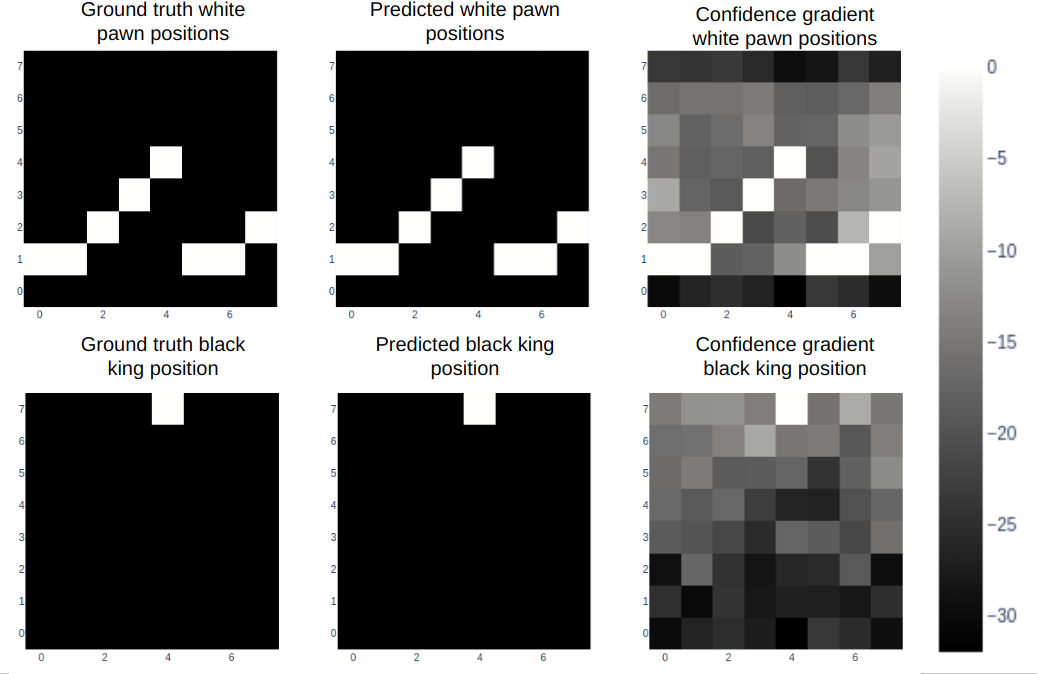
\includegraphics[width=0.85\textwidth]
        {figures/latent_space_analysis/probing_illustration.png}
    \caption[Probing analysis of a chess-playing language model.]{
        Probing analysis of an \glsfmtshort{llm} trained to play chess
        \parencite{karvonen2024emergentworldmodelslatent}.
    }
    \label{fig:probing_illustration}
\end{figure}

However, the fact that a concept can be decoded from \glspl{lr} does not necessarily imply that the model actually uses this information to perform its task.
To assess whether \glspl{lr} play a causal role in the model's output, it is possible to perform interventions on them.
An intervention consists of modifying a \gls{lr} in a controlled manner by activating or deactivating a given concept, and then studying its impact on the model's output.
If the resulting change in the model's output is consistent with the applied perturbation, this suggests that the representation had a causal role.

To this end, the \gls{lr} is minimally modified such that the probe prediction for the target concept $c_j$ changes state, while the predictions associated with other concepts remain unchanged.
This goal can be formulated as an optimization problem over the \gls{lr} itself.
The optimization is performed directly on the \gls{lr}, using \gls{sgd}.
The solution to this problem is the optimal modified \gls{lr}, defined as:
\[
\begin{aligned}
\latentRepresentation[l][*] =
\argmin_{\latentRepresentation[l][\prime]} \;
&\underbrace{\lambda_1 \, \mathcal{L}_{\mathrm{flip}}\big(\Probe{l}{j}(\latentRepresentation[l][\prime]), c_j\big)}_{\text{flip target concept } c_j} \\
+ \, &\underbrace{\lambda_2 \sum_{k \neq j} \mathcal{L}_{\mathrm{preserve}}\big(\Probe{l}{k}(\latentRepresentation[l][\prime]), c_k\big)}_{\text{preserve other concepts } c_{k \neq j}} \\
+ \, &\underbrace{\lambda_3 \|\latentRepresentation[l][\prime] - \latentRepresentation[l]\|_2^2}_{\text{minimality}},
\end{aligned}
\]
where:
\begin{itemize}
    \item $\latentRepresentation[l]$ is the original \gls{lr} of the input at layer $l$,
    \item $\latentRepresentation[l][\prime]$ is the modified \gls{lr} being optimized,
    \item $\latentRepresentation[l][*]$ is the optimal modified \gls{lr},
    \item $\mathcal{L}_{\mathrm{flip}}$: loss encouraging the prediction of the target concept $c_j$ to change state (i.e., flipping the predicted label),
    \item $\mathcal{L}_{\mathrm{preserve}}$: loss enforcing invariance of all non-target concepts $c_k$ for $k \neq j$,
    \item $\|\latentRepresentation[l][\prime] - \latentRepresentation[l]\|_2^2$: regularization term ensuring the modified \gls{lr} remains close to the original one,
    \item $\lambda_1, \lambda_2, \lambda_3$: weighting coefficients controlling the trade-off between the intervention strength, the preservation of other concepts, and the minimality of the perturbation.
\end{itemize}

In the context of \glspl{llm} studied previously, such interventions have been used to remove specific pieces from the model's internal representation of the game state \parencite{li2024emergentworldrepresentationsexploring, karvonen2024emergentworldmodelslatent}.
The main observation is that, in the vast majority of cases, the model behaves as if the piece had effectively disappeared.
The \gls{llm} continues to generate legal moves while correctly accounting for the absence of the removed piece.
This provides evidence for the causal role of these internal representations in the model's behavior.

A main limitation of the probing approach is that the concepts under investigation must be predefined before any analysis can be performed.
This introduces a strong bias.
Moreover, annotating a dataset for each concept is extremely time-consuming.
Interventions in \gls{ls} are also difficult to interpret, as it is not always clear what constitutes a meaningful change in the network's output under a given perturbation.

Finally, probing methods provide a binary view of concepts, focusing on whether a given concept is present or absent in a \gls{lr}.
This binary perspective can be restrictive, as concepts may be represented in a more continuous manner.

To obtain a more detailed characterization of these representations, the next section turns to methods that describe a concept as a direction in \gls{ls} along which it varies continuously.
\section{Directions}
\label{sec:latent_space_analysis_directions}

Probing describes a concept as a binary attribute, either present or absent in a \gls{lr}.
The methods in this section instead associate each concept with a direction in the \gls{ls}.
Moving a \gls{lr} along this direction is expected to strengthen or weaken the concept smoothly.
This provides information that a binary probe cannot express.

Empirically, it has been observed that shifting a \gls{lr} along such a direction can induce coherent and semantically meaningful changes in the model's output \parencite{haas2024discovering, voynov2020unsuperviseddiscoveryinterpretabledirections}.
Such a shift is a latent intervention (see Definition~\ref{def:latent_intervention}) and can be expressed mathematically as:
\begin{equationwhere}
\[
\latentRepresentation' = \latentRepresentation + \alpha \vect{v}_i,
\]
where:
\begin{itemize}
    \item $\latentRepresentation$ denotes the original \gls{lr},
    \item $\vect{v}_i$ is a unit vector associated with concept $i$,
    \item $\alpha$ controls the strength of the intervention,
    \item $\latentRepresentation'$ is the resulting perturbed \gls{lr}.
\end{itemize}
\end{equationwhere}

In many cases, the resulting change in the model's output varies smoothly with \(\alpha\), suggesting an approximately linear \gls{cs} with respect to certain semantic factors.
This observation has led to the hypothesis that neural representations may organize concepts in a partially linear manner within the \gls{ls}.

Vectors of this form are referred to as interpretable directions, as they correspond to transformations that can be associated with specific semantic attributes.
The objective of this line of work is therefore to identify directions in \gls{ls} that align with meaningful variations in the encoded concepts.
This is illustrated schematically in Figure~\ref{fig:latent_directions}, where arrows represent semantic shifts from one concept toward others, and moving along these directions induces a coherent change in the model's behavior, suggesting that the transition between concepts is continuously encoded along these axes.

\begin{figure}[t]
\centering

\input{figures/latent_space_analysis/latent_space_shared.tex}

\resizebox{0.65\textwidth}{!}{
\begin{tikzpicture}
\begin{axis}[latent axis]

  % Point clouds
  \plotPoints[color=colorA, mark=*]{figures/latent_space_analysis/cluster_a.data}
  \plotPoints[color=colorB, mark=square*]{figures/latent_space_analysis/cluster_b.data}
  \plotPoints[color=colorC, size=2pt, mark=triangle*]{figures/latent_space_analysis/cluster_c.data}

  % Interpretable directions
  \plotProbe[color=colorDirBA, style=dashed, width=thick]{-11}{-31.5}
  \plotDirection[color=colorDirBA]{-2.5}{-4.0}{-3.0}{1.5}

  \plotProbe[color=colorDirBC, style=dashed, width=thick]{0.5224}{-2.694}
  \plotDirection[color=colorDirBC]{-2.5}{-4.0}{4.2}{-0.5}

  % Centroid B
  \fill[colorB] (axis cs:-2.5,-4.0) circle (4pt);

\end{axis}
\end{tikzpicture}
}

\caption{
    Interpretable directions in the \glsfmtshort{ls}.
}
\label{fig:latent_directions}
\end{figure}


This phenomenon has been extensively studied in generative image models.
Controlled perturbations of \glspl{lr} along interpretable directions can induce specific semantic transformations \parencite{voynov2020unsuperviseddiscoveryinterpretabledirections}.
Examples include stroke thickness modification in digit images, head rotation in facial images, and texture or background changes in natural images.
These transformations are illustrated in Figure~\ref{fig:interpretable_direction_illustration}, where each row corresponds to a distinct direction $\vect{v}_i$ and each column to an increasing value of $\alpha$.
These observations have led to the development of the field of \gls{ls} editing, whose objective is to manipulate generated content directly through modifications in \gls{ls} rather than through changes in the input prompt.

% figures/latent_space_analysis/interpretable_direction_illustration.tex

\begin{figure}[t]
    \centering
    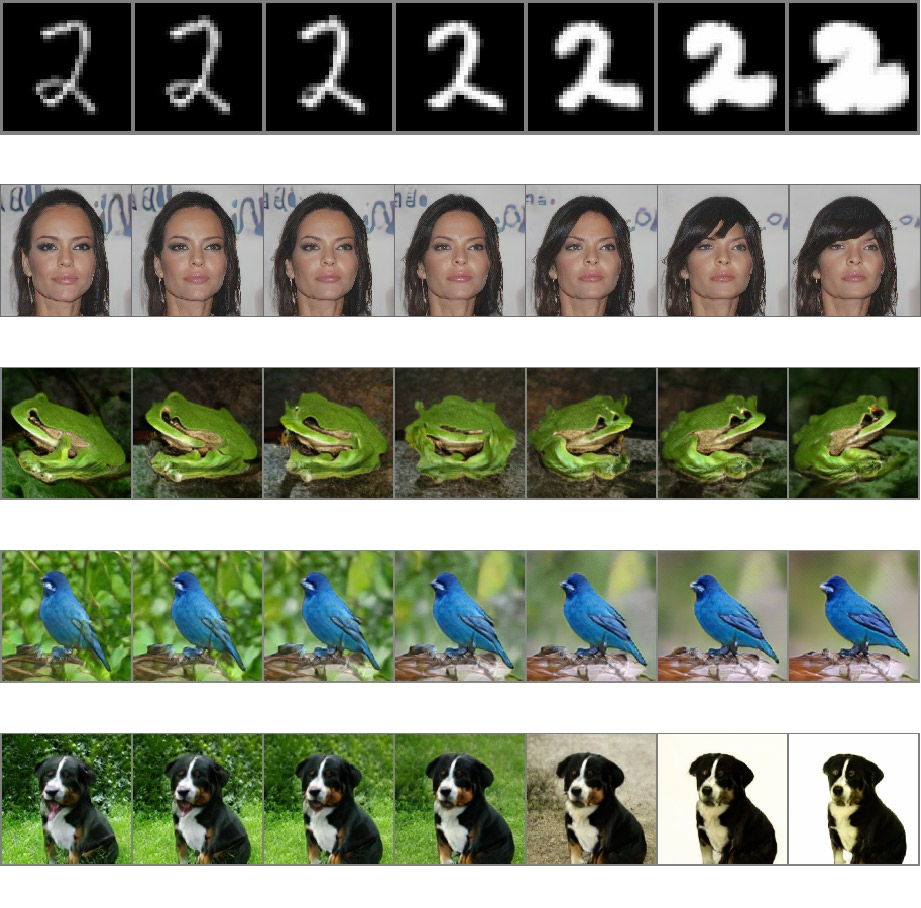
\includegraphics[width=0.85\textwidth]
        {figures/latent_space_analysis/interpretable_direction_illustration.png}
    \caption[Interpretable directions in the latent space of a generative model.]{
        Interpretable directions in the latent space of a generative model \parencite{voynov2020unsuperviseddiscoveryinterpretabledirections}.
    }
    \label{fig:interpretable_direction_illustration}
\end{figure}

A central challenge remains identifying such interpretable directions.
Most existing approaches rely on auxiliary models that encode human defined semantics, such as CLIP \parencite{haas2024discovering}, to relate latent variations to textual concepts.
Consequently, these methods inherit a limitation similar to that of probing techniques, since concept discovery depends on a pre-existing semantic framework defined by humans.

To overcome this limitation, a research direction known as unsupervised semantic discovery has emerged.
Its goal is to uncover interpretable directions in \gls{ls} without explicit semantic supervision.
In these approaches, one model applies perturbations along random directions in \gls{ls}, while a second model attempts to recognize the applied transformation.
If a stable correspondence emerges between the perturbation and its prediction, this suggests that the considered direction corresponds to a coherent \gls{cs} \parencite{voynov2020unsuperviseddiscoveryinterpretabledirections}.
In this framework, human intervention occurs only a posteriori, to verify whether the discovered directions indeed correspond to interpretable semantic variations.

Despite these advances, several challenges remain.
It appears that not all concepts encoded by \glspl{nn} are linearly identifiable in \gls{ls}.
In addition, \glspl{lr} often exhibit a phenomenon known as entanglement, illustrated in Figure~\ref{fig:entanglement_illustration}, where multiple semantic attributes are mixed within the same directions of the \gls{ls}.
For instance, in a generative face model, moving along the \enquote{glasses} direction may simultaneously modify age and gender, whereas a disentangled \gls{lr} would let each axis control a single semantic attribute while leaving the others unchanged.

This lack of separability suggests that semantic information is not cleanly organized in the \gls{ls}.
This observation motivates the \SuperpositionHypothesisName, which proposes a different view of how \glspl{nn} organize information internally.
The next section introduces this hypothesis.

\begin{figure}[t]
    \centering
    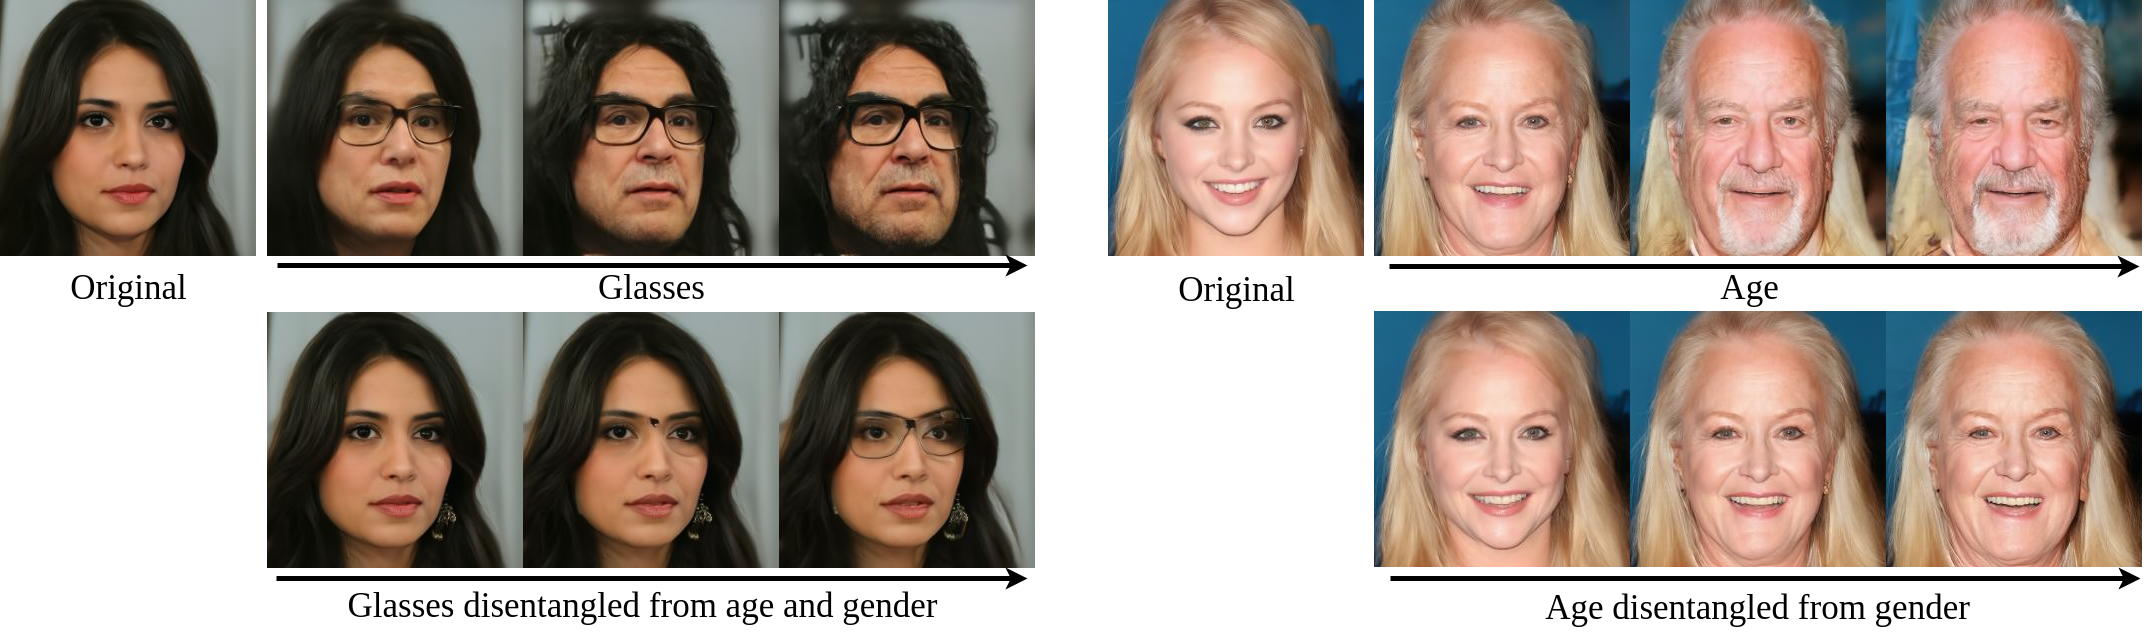
\includegraphics[width=0.85\textwidth]
        {figures/latent_space_analysis/entanglement_illustration.png}
    \caption[Entanglement in the latent space of a generative face model.]{
        Illustration of entanglement in the latent space of a generative face
        model \parencite{haas2024discovering}.
    }
    \label{fig:entanglement_illustration}
\end{figure}
\section{Superposition}
\label{sec:latent_space_analysis_superposition}

The previous section highlighted a limitation of interpretable directions.
Only a limited number of concepts can be represented by a linear direction, and these directions are often entangled with multiple semantic concepts.
To account for this, an extension of the \ConceptHypothesisName has been proposed under the name \SuperpositionHypothesisName, formalized in Hypothesis~\ref{hyp:superposition} \parencite{elhage2022superposition}.

\begin{hypothesis}{Superposition Hypothesis}{superposition}
Concepts are preferentially represented by distinct linear directions in \gls{ls}.
When the number of concepts exceeds the available dimensions, multiple concepts are encoded in superposition within the same directions.
\end{hypothesis}

According to this hypothesis, in an unconstrained \gls{ls}, each concept is represented in its own independent linear direction.
The idealized non-superposed \gls{lr} can be mathematically expressed as follows:
\[
\latentRepresentation = \sum_{i=1}^{n} \alpha_i \vect{v}_i,
\qquad
\forall i \neq j,\quad \vect{v}_i^\top \vect{v}_j \approx 0,
\qquad
\|\boldsymbol{\alpha}\|_0 \ll n,
\]

where:
\begin{itemize}
    \item $\latentRepresentation$ denotes a \gls{lr},
    \item $n$ is the total number of concepts,
    \item $\vect{v}_i$ represents the direction associated with concept $c_i$,
    \item $\alpha_i$ corresponds to the activation strength of concept $c_i$ in the \gls{lr} $\latentRepresentation$,
    \item $\vect{v}_i^\top \vect{v}_j \approx 0$ indicates that concept directions are approximately orthogonal, meaning each concept independently controls a single factor of variation,
    \item $\|\boldsymbol{\alpha}\|_0 \ll n$ indicates that only a small fraction of concepts are active for a given \gls{lr}.
\end{itemize}

However, \glspl{nn} operate in finite-dimensional spaces, so when the number of concepts exceeds the available dimensions, such a one-to-one correspondence becomes impractical.
The network must therefore reuse its representational dimensions, allowing multiple concepts to be encoded using the same directions.
This shared encoding is referred to as superposition \parencite{bricken2023monosemanticity}.
This phenomenon becomes an obstacle for any method that attempts to analyze \glspl{lr} directly in the original activation space.

Building on this observation, several works based on the \SuperpositionHypothesisName have developed methods that aim to recover less superposed \glspl{lr}.
A common approach is to map \gls{ls} into a higher-dimensional space while imposing additional constraints that encourage individual concepts to be represented separately.
This transformation is illustrated in Figure~\ref{fig:dense_to_sparse_sae}, while \glspl{lr} are entangled in the initial \gls{ls}, the sparse representation aligns each concept with a dedicated feature axis.

\providecommand{\lsePanelWidth}{6cm}
\newlength{\saePanelWd}
\newlength{\saePanelHt}
\newlength{\saePanelGap}

% Lengths must be set BEFORE \resizebox so pgfplots sees non-zero values.
\setlength{\saePanelWd}{\lsePanelWidth}
\pgfmathsetlength{\saePanelHt} {\saePanelWd * 5 / 6}
\pgfmathsetlength{\saePanelGap}{\saePanelWd * 0.9}

\begin{figure}[t]
\centering

\input{figures/latent_space_analysis/latent_space_shared.tex}

\resizebox{1\textwidth}{!}{
\begin{tikzpicture}

  % ================================================================
  % LEFT PANEL — Dense latent space
  % ================================================================
  \begin{scope}[xshift=0pt]
  \begin{axis}[
    name=axisLeft,
    latent embed,
    width=\saePanelWd,
    height=\saePanelHt,
    xmin=-7, xmax=8,
    ymin=-7, ymax=5.5,
  ]
    \plotPoints[color=colorA, mark=*]{figures/latent_space_analysis/cluster_a.data}
    \plotPoints[color=colorB, mark=square*]{figures/latent_space_analysis/cluster_b.data}
    \plotPoints[color=colorC, size=2pt, mark=triangle*]{figures/latent_space_analysis/cluster_c.data}
    \end{axis}
    \node[anchor=north, yshift=-6pt] at (axisLeft.south)
      {(a) Dense latent space};
  \end{scope}

  % ================================================================
  % RIGHT PANEL — Sparse SAE space
  % ================================================================
  \begin{scope}[xshift=\saePanelGap]
  \begin{axis}[
    name=axisRight,
    width=\saePanelWd,
    height=\saePanelHt,
    xmin=-8.5, xmax=8.5,
    ymin=-6,   ymax=9,
    axis lines=none,
    ticks=none,
    clip=true,
  ]

    \draw[colorA, thick, -{Stealth[length=7pt,width=5pt]}]
      (axis cs:0,0) -- (axis cs:0,7);
    \node[colorA, font=\small\bfseries, above] at (axis cs:0,7.3)
      {Feature $A$};

    \draw[colorB, thick, -{Stealth[length=7pt,width=5pt]}]
      (axis cs:0,0) -- (axis cs:-6.062,-3.5);
    \node[colorB, font=\small\bfseries, below left] at (axis cs:-6.062,-3.8)
      {Feature $B$};

    \draw[colorC, thick, -{Stealth[length=7pt,width=5pt]}]
      (axis cs:0,0) -- (axis cs:6.062,-3.5);
    \node[colorC, font=\small\bfseries, below right] at (axis cs:6.062,-3.8)
      {Feature $C$};

    \plotPoints[color=colorA, mark=*]{figures/latent_space_analysis/sae_right_a.data}
    \plotPoints[color=colorB, mark=square*]{figures/latent_space_analysis/sae_right_b.data}
    \plotPoints[color=colorC, size=2pt, mark=triangle*]{figures/latent_space_analysis/sae_right_c.data}

  \end{axis}
  \node[anchor=north, yshift=-6pt] at (axisRight.south)
    {(b) Sparse SAE space};
  \end{scope}

\end{tikzpicture}
}

\caption[Transformation from a dense to a sparse \glsfmtshort{ls}.]{
  Transformation from a dense \glsfmtshort{ls}~(a) to a sparse
  \glsfmtshort{sae} representation~(b).
}
\label{fig:dense_to_sparse_sae}
\end{figure}


\glspl{sae} provide a practical implementation of this approach and can be defined as follows:
\[
\vect{z} = \Encoder(\latentRepresentation), \quad \hat{\latentRepresentation} = \Decoder(\vect{z})
\]
\[
\mathcal{L}_{\mathrm{auto}} = \|\latentRepresentation - \hat{\latentRepresentation}\|_2^2 + \lambda \|\vect{z}\|_1
\]

where:
\begin{itemize}
    \item $\Encoder(\latentRepresentation)$ is the encoding function that projects the original \gls{lr} $\latentRepresentation$ into a higher-dimensional sparse space,
    \item $\Decoder(\vect{z})$ is the decoding function that reconstructs the original \gls{lr} from the sparse code,
    \item $\vect{z} \in \mathcal{Z}$ is the sparse representation of $\latentRepresentation$, with $\dim(\vect{z}) \gg \dim(\latentRepresentation)$,
    \item $\hat{\latentRepresentation}$ is the reconstructed \gls{lr},
    \item $\|\latentRepresentation - \hat{\latentRepresentation}\|_2^2$ is the reconstruction loss ensuring that the original \gls{lr} can be faithfully recovered,
    \item $\|\vect{z}\|_1$ is the sparsity regularization term that encourages most components of $\vect{z}$ to be zero,
    \item $\lambda$ is a weighting coefficient controlling the trade-off between reconstruction fidelity and sparsity.
\end{itemize}

The parameters of these projection functions $\Encoder$ and $\Decoder$ are learned by minimizing $\mathcal{L}_{\mathrm{auto}}$ using \gls{sgd}.
Under this formulation, each dimension of $\mathcal{Z}$ is interpreted as a dedicated concept direction.

In practice, both $\Encoder$ and $\Decoder$ are implemented as linear projections between the original \gls{ls} and the high-dimensional space $\mathcal{Z}$. This choice is motivated by the same principle underlying probing methods. The transformation applied to the \gls{lr} should remain as simple as possible.
Using more expressive projection functions could introduce additional structures into the transformed \gls{lr}. In this case, it would become difficult to determine whether an observed concept was already encoded in the model's \gls{lr}, or whether it was introduced by the projection itself. Restricting $\Encoder$ and $\Decoder$ to linear projections therefore helps ensure that the concepts identified in $\mathcal{Z}$ can be attributed to the original \gls{lr}, rather than to the transformation used to analyze it.

The method proves to be powerful when successfully applied to language models \parencite{templeton2024scaling}.
In these applications, \glspl{sae} are used to desuperpose the \gls{lr} of \glspl{llm}.
Once this \gls{lr} is obtained, it has been shown that many concept vectors exhibit semantic properties.
A example is the Golden Gate Bridge concept direction, illustrated in Figure~\ref{fig:sparse_autoencoder_illustration}, which activates systematically whenever the input text or image refers to the Golden Gate Bridge, regardless of the language or modality.
This demonstrates that the learned concept is not tied to a specific surface form but captures a deeper semantic abstraction shared across modalities.

\begin{figure}[t]
    \centering
    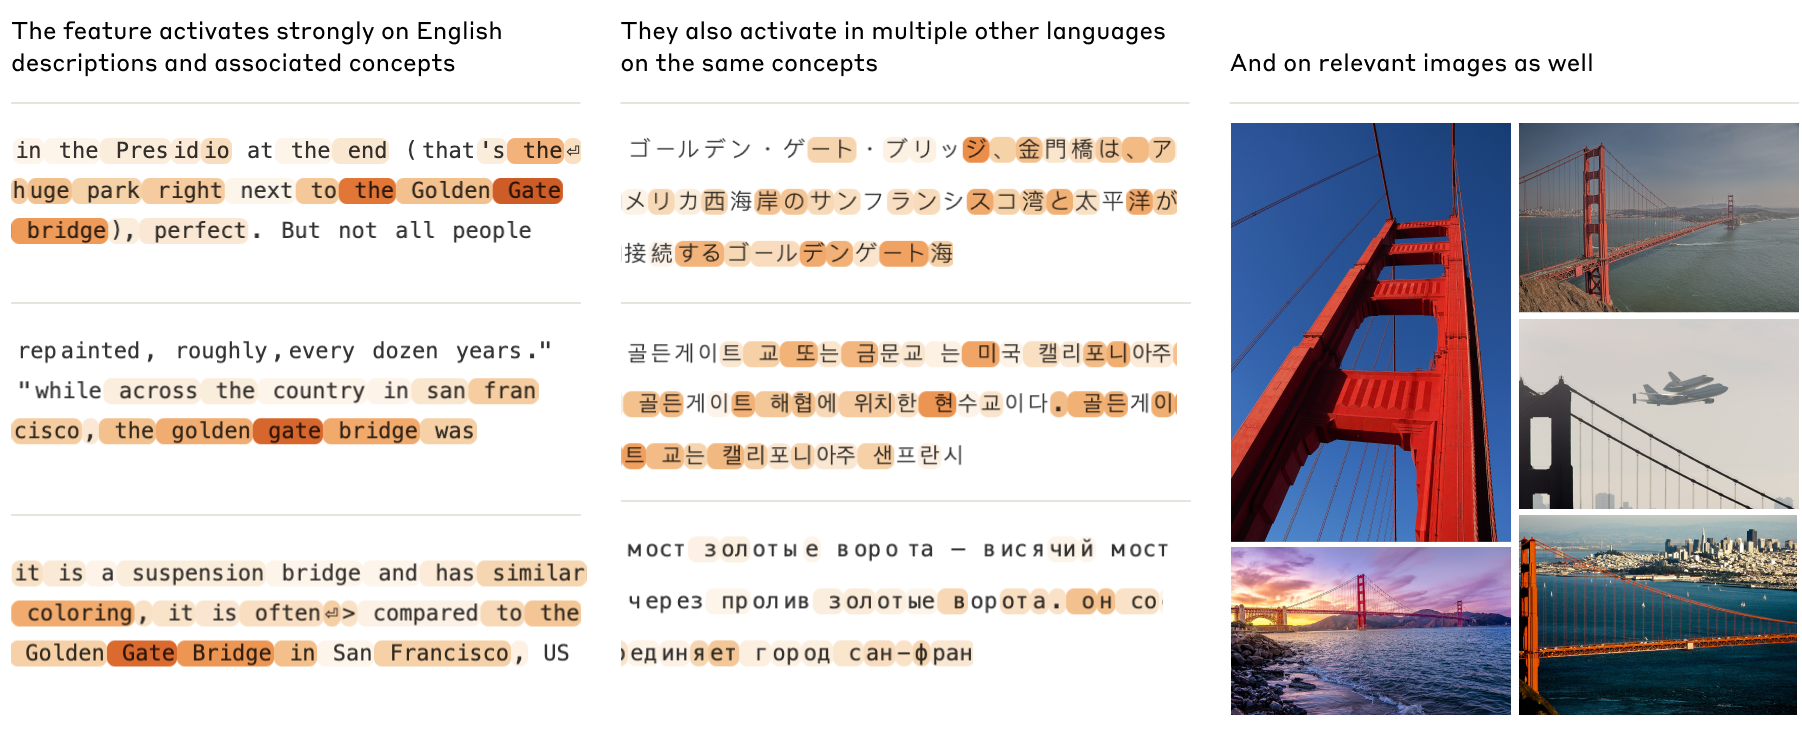
\includegraphics[width=0.85\textwidth]
        {figures/latent_space_analysis/sparse_autoencoder_illustration.png}
    \caption[The Golden Gate Bridge concept direction of an \glsfmtshort{sae}.]{
        A concept direction corresponding to the Golden Gate Bridge, discovered
        by an \glsfmtshort{sae} applied to an \glsfmtshort{llm}
        \parencite{templeton2024scaling}.
    }
    \label{fig:sparse_autoencoder_illustration}
\end{figure}

\glspl{sae} also provide a way to intervene directly on the \gls{lr} learned by the model.
A concept can be artificially activated by modifying its corresponding feature in the sparse representation $\vect{z}$, even when the input contains no reference to it.
The modified \gls{lr} is then projected back into the original activation space, after which the model proceeds with standard next-token generation from $\latentRepresentation^{*}$:
\[
\latentRepresentation^{*} = \Decoder(\vect{z}^*), \quad \text{where} \quad \vect{z}^* = \vect{z} + \alpha \, \vect{e}^{(i)},
\]

where:
\begin{itemize}
    \item $\vect{z}$ is the original sparse representation of the input,
    \item $\vect{z}^*$ is the modified sparse representation,
    \item $\vect{e}^{(i)}$ is the basis vector of $\mathcal{Z}$ associated with the target concept direction,
    \item $\alpha$ controls the strength of the artificial activation,
    \item $\latentRepresentation^{*}$ is the resulting edited \gls{lr} in the original activation space.
\end{itemize}

With this method, a reference to the Golden Gate Bridge can be injected into the \gls{llm}'s internal representation.
This causes the model's output to shift toward discussing the Golden Gate Bridge, even when the prompt contains no reference to it.
This provides evidence that the learned feature plays a causal role in the model's behavior.
Such interventions enable control over specific model behaviors through \gls{ls} editing.

Despite their empirical success, \SuperpositionHypothesisName exhibit several important limitations that question their assumptions. 
These limitations can be summarized as follows:
\begin{itemize}
    \item \textbf{Instability of the decomposition.}
    Repeating the \gls{sae} training process multiple times on the same model does not yield the same decomposition of the \gls{ls}.
    Different runs produce different concept directions in $\mathcal{Z}$, even when achieving comparable reconstruction performance, which raises questions about the reliability of the discovered \glspl{cs}.

    \item \textbf{Lack of semantic coverage.}
    In the high-dimensional space $\mathcal{Z}$, a large fraction of dimensions do not correspond to any interpretable semantic concept.
    This abundance of non-semantic directions raises questions about whether the decomposition truly reflects the model's \glspl{cs}.

    \item \textbf{Sparsity--semantics trade-off.}
    Increasing the sparsity coefficient $\lambda$ beyond a certain threshold degrades the semantic quality of the learned features \parencite{tanhPenaltyDictionaryLearning}.
    Suggesting that enforcing excessive sparsity comes at the cost of interpretability.

    \item \textbf{Failure of scaling to remove superposition.}
    Under the \SuperpositionHypothesisName, increasing the dimensionality of the \gls{ls} should reduce superposition.
    However, this is not observed in practice.
    Even in very high-dimensional \glspl{ls}, representations remain superposed, indicating that scaling alone does not resolve the entanglement.
\end{itemize}

These limitations suggest that \SuperpositionHypothesisName, while powerful, do not fully resolve the problem of \gls{cs}.
Convincing empirical results do not necessarily validate the underlying theoretical assumptions.

So far, every method described, whether based on probing, interpretable directions, or superposition, relies on a common assumption.
The \gls{cs} can be recovered from \glspl{lr} through a linear decomposition.
This assumption has enabled substantial progress in understanding neural representations, but it also imposes a strong constraint on how concepts are expected to be represented.
The following section examines clustering as an alternative approach that does not rely on this assumption.
\section{Clustering}
\label{sec:latent_space_analysis_clustering}

As the previous section noted, every \gls{ls} analysis method presented so far rests on a linear view of the \gls{cs}.
For probing methods, concepts must be at least partially linearly separable for simple probes to detect them.
Interpretable direction methods posit that variations associated with a concept can be captured by moving along a linear axis of the \gls{ls}.
The \SuperpositionHypothesisName proposes that concepts are represented through linear directions that become entangled because of representational capacity constraints.

Although these assumptions have led to empirical successes, several observations suggest that the linearity hypothesis may not fully capture the \gls{cs}.
For instance, some concepts can only be recovered using non-linear probes.
Likewise, methods based on interpretable directions typically identify only a limited number of semantic factors.
Finally, in \gls{sae} approaches, enforcing excessive sparsity degrades interpretability.
This suggests that the underlying representation may not be perfectly described by a sparse linear decomposition.
Taken together, these observations indicate that semantic concepts may not always exhibit a linear \gls{cs}.
This motivates the exploration of alternative approaches that rely on weaker assumptions regarding the geometry of \glspl{ls}.

To the best of our knowledge, clustering-based analysis is the only family of \gls{ls} analysis methods that does not rely on any assumption of a linear \gls{cs} \parencite{ren_deep_2022, wei_overview_2024}.
Rather than assuming that concepts correspond to directions, clustering methods only assume that conceptual similar inputs produce nearby \glspl{lr}.
Conversely, inputs that differ significantly from a concept perspective are expected to be located farther apart in the \gls{ls}.
This is a considerably weaker assumption, in the sense that it is empirically verified in a wide range of settings.

Under this assumption, the discovery of concepts can be reformulated as the identification of groups of \glspl{lr} that occupy the same region of the \gls{ls}.
This is shown schematically in Figure~\ref{fig:latent_clusters}, where the points represent \glspl{lr} associated with concepts, and the ellipses indicate the approximate extent of each group and highlight their geometric separation.

\begin{figure}[t]
\centering

\input{figures/latent_space_analysis/latent_space_shared.tex}

\resizebox{0.65\textwidth}{!}{
\begin{tikzpicture}
\begin{axis}[latent axis]

  % Cluster boundaries
  \plotEllipse[color=colorA, width=very thick, fill=colorA, fillopacity=0.08]
    {-3}{1.5}{15}{2.3}{1.2}
  \plotEllipse[color=colorB, width=very thick, fill=colorB, fillopacity=0.08]
    {-2.5}{-4}{10}{2.2}{1.1}
  \plotEllipse[color=colorC, width=very thick, fill=colorC, fillopacity=0.08]
    {4.2}{-0.5}{-20}{1.4}{2.6}

  % Point clouds
  \plotPoints[color=colorA, mark=*]{figures/latent_space_analysis/cluster_a.data}
  \plotPoints[color=colorB, mark=square*]{figures/latent_space_analysis/cluster_b.data}
  \plotPoints[color=colorC, size=2pt, mark=triangle*]{figures/latent_space_analysis/cluster_c.data}

\end{axis}
\end{tikzpicture}
}

\caption{
  Visualization of the \glsfmtshort{ls} structure.
}
\label{fig:latent_clusters}
\end{figure}


This idea forms the basis of the research field known as deep clustering.
In these approaches, a collection of inputs is projected into a \gls{ls} using a \gls{nn}.
The resulting \glspl{lr} form a point cloud on which standard clustering algorithms can be applied.
The obtained clusters are then interpreted as representing distinct concepts.

Deep clustering has been particularly successful in unsupervised image classification.
For this type of task, a specific \gls{nn} architecture called an autoencoder is commonly used.
An autoencoder is composed of an encoder $\Encoder$ and a decoder $\Decoder$.
The encoder maps an input $\vect{x} \in \mathcal{X}$ to a low-dimensional \gls{lr} $\vect{z} \in \mathbb{R}^d$, the \gls{lr} produced by the encoder.
The decoder then maps this \gls{lr} back to the input space to produce a reconstruction $\hat{\vect{x}}$.

The model is trained by \gls{sgd} to minimize the reconstruction error between the original input and its reconstruction using a \gls{mse} loss.
This objective encourages the \gls{ls} to preserve the most informative features of the input while enforcing a compact representation.
This can be expressed mathematically as follows:
\[
\vect{x}
\xrightarrow{\;\Encoder\;}
\vect{z}
\xrightarrow{\;\Decoder\;}
\hat{\vect{x}},
\qquad
d \ll \dim(\mathcal{X}),
\qquad
\mathcal{L}_{\mathrm{rec}}
=
\frac{1}{N}\sum_{i=1}^{N}
\left\|\vect{x}^{(i)}-\hat{\vect{x}}^{(i)}\right\|_2^2.
\]

Once the autoencoder has been trained sufficiently well, the reconstruction loss $\mathcal{L}_{\mathrm{rec}}$ should be low enough for the learned representation to be useful.
A clustering algorithm can then be applied to the compressed representations of the images.
Let $\mathcal{D}$ denote a dataset of inputs, through the encoder $\Encoder$, this dataset is mapped to a point cloud in the \gls{ls}:
\[
\mathcal{Z} = \{\vect{z}^{(i)} \in \mathbb{R}^d \mid \vect{z}^{(i)} = \Encoder(\vect{x}^{(i)}), \; \vect{x}^{(i)} \in \mathcal{D} \}.
\]

A classical clustering algorithm is applied to the set $\mathcal{Z}$ of \glspl{lr} to identify groups of similar \glspl{lr}.
Each resulting cluster can therefore be interpreted as a group of images that the model considers similar.

An example of this methodology can be observed in Figure~\ref{fig:deep_clustering_illustration}, where the approach is applied to the STL-10 dataset \parencite{coates2011analysis} using $k$-means clustering \parencite{macqueen1967multivariate} with a number of clusters arbitrarily fixed to $K = 10$ \parencite{xie_unsupervised_2016}.
For each cluster, the corresponding line shows the $10$ samples closest to the associated centroid in the \gls{ls}.
We observe that the method captures coherent semantic categories such as animals, vehicles, and flying entities.

\begin{figure}[t]
    \centering
    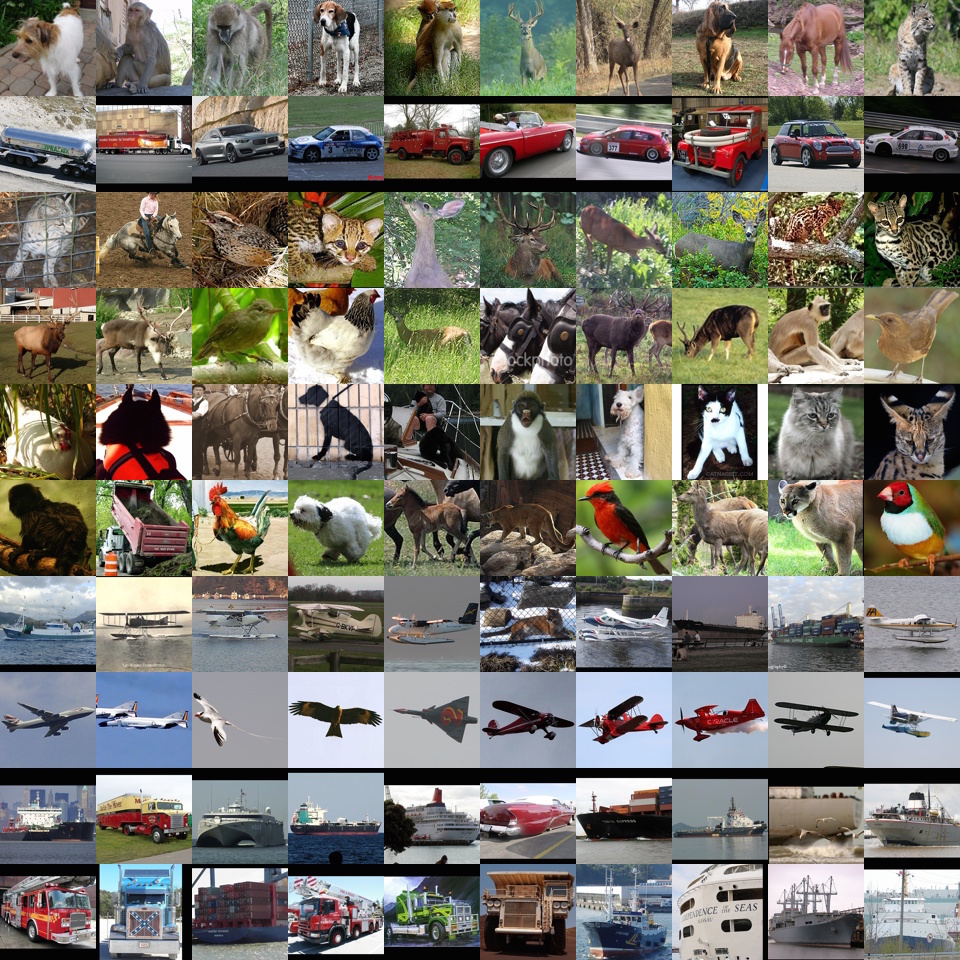
\includegraphics[width=0.85\textwidth]
        {figures/latent_space_analysis/deep_clustering_illustration.jpg}
    \caption[Clusters discovered by deep clustering on natural images.]{
        Clusters discovered by a deep clustering model applied to natural images \parencite{xie_unsupervised_2016}.
    }
    \label{fig:deep_clustering_illustration}
\end{figure}

This result is particularly striking given that the only available information to the system consists of raw images.
It suggests that the compression process induces a \gls{ls} in which semantically meaningful \glspl{cs} emerge.

More advanced approaches combine representation learning and clustering within a single optimization process.
In this setting, additional loss terms encourage \glspl{lr} to organize themselves around cluster centroids during training.
This often produces \glspl{ls} that are easier to analyze and improves the quality of the discovered semantic \glspl{cs} \parencite{guo_improved_2017, miklautz_breaking_2024}.

Clustering-based analysis presents several important limitations.
First, as with most unsupervised semantic discovery techniques, interpreting the resulting clusters remains partly subjective.
Benchmark datasets often provide class labels for evaluation, but the discovered clusters may not match the categories that humans consider relevant. 

Second, clustering methods are highly sensitive to design choices.
The number of clusters, the distance metric, and the clustering algorithm itself can all significantly influence the results.
Parameter selection is therefore challenging and often requires substantial empirical tuning.

Finally, to the best of our knowledge, no intervention technique has yet been proposed in the context of clustering-based analysis.
Unlike probing or \gls{sae} analysis, which allow targeted modifications of \glspl{lr} to study their causal role, clustering methods currently offer no mechanism to alter the model's behavior by acting directly on the discovered \glspl{cs}.

\section{Conclusion}
\label{sec:latent_space_analysis_conclusion}

% figures/latent_space_analysis/latent_space_overview.tex

\providecommand{\lsePanelWidth}{5.5cm}
\newlength{\ovPanelWd}
\newlength{\ovPanelHt}
\newlength{\ovPanelGap}
\newlength{\ovRowGap}

\setlength{\ovPanelWd}{\lsePanelWidth}
\pgfmathsetlength{\ovPanelHt} {\ovPanelWd * 5 / 6}
\pgfmathsetlength{\ovPanelGap}{\ovPanelWd * 1}
\pgfmathsetlength{\ovRowGap}  {\ovPanelHt * 1}

\begin{figure}[t]
\centering

\input{figures/latent_space_analysis/latent_space_shared.tex}

\resizebox{\textwidth}{!}{
\begin{tikzpicture}

  % ============================================================
  % (a) TOP-LEFT — Probing
  % ============================================================
  \begin{scope}[xshift=0pt, yshift=0pt]
  \begin{axis}[
    name=axisProbing,
    latent embed, width=\ovPanelWd, height=\ovPanelHt,
  ]
    \fill[colorA, opacity=0.10]
      (axis cs:-7,-4) -- (axis cs:-7,5.5) -- (axis cs:2.5,5.5) -- cycle;
    \fill[colorB, opacity=0.10]
      (axis cs:-7,0.1) -- (axis cs:8,-4.4) --
      (axis cs:8,-7)   -- (axis cs:-7,-7)  -- cycle;
    \fill[colorC, opacity=0.10]
      (axis cs:-0.75,5.5) -- (axis cs:8,5.5) --
      (axis cs:8,-7)      -- (axis cs:5.5,-7) -- cycle;
    \plotProbe[color=colorA]{1}{3}
    \plotProbe[color=colorB]{-0.3}{-2}
    \plotProbe[color=colorC]{-2}{4}
    \plotPoints[color=colorA, mark=*]{figures/latent_space_analysis/cluster_a.data}
    \plotPoints[color=colorB, mark=square*]{figures/latent_space_analysis/cluster_b.data}
    \plotPoints[color=colorC, size=2pt, mark=triangle*]{figures/latent_space_analysis/cluster_c.data}
  \end{axis}
  \node[anchor=north, yshift=-6pt] at (axisProbing.south)
    {\textbf{(a)} Probing};
  \end{scope}

  % ============================================================
  % (b) TOP-RIGHT — Directions
  % ============================================================
  \begin{scope}[xshift=\ovPanelGap, yshift=0pt]
  \begin{axis}[
    name=axisDirections,
    latent embed, width=\ovPanelWd, height=\ovPanelHt,
  ]
    \plotPoints[color=colorA, mark=*]{figures/latent_space_analysis/cluster_a.data}
    \plotPoints[color=colorB, mark=square*]{figures/latent_space_analysis/cluster_b.data}
    \plotPoints[color=colorC, size=2pt, mark=triangle*]{figures/latent_space_analysis/cluster_c.data}
    \plotProbe[color=colorDirBA, style=dashed, width=thick]{-11}{-31.5}
    \plotDirection[color=colorDirBA]{-2.5}{-4.0}{-3.0}{1.5}
    \plotProbe[color=colorDirBC, style=dashed, width=thick]{0.5224}{-2.694}
    \plotDirection[color=colorDirBC]{-2.5}{-4.0}{4.2}{-0.5}
    \fill[colorB] (axis cs:-2.5,-4.0) circle (4pt);
  \end{axis}
  \node[anchor=north, yshift=-6pt] at (axisDirections.south)
    {\textbf{(b)} Directions};
  \end{scope}

  % ============================================================
  % (c) BOTTOM-LEFT — Superposition
  % ============================================================
  \begin{scope}[xshift=0pt, yshift=-\ovRowGap]
  \begin{axis}[
    name=axisSAE,
    width=\ovPanelWd, height=\ovPanelHt,
    xmin=-8.5, xmax=8.5, ymin=-6, ymax=9,
    axis lines=none, ticks=none, clip=true,
  ]
    \draw[colorA, thick, -{Stealth[length=5pt,width=4pt]}]
      (axis cs:0,0) -- (axis cs:0,7);
    \node[colorA, font=\small\bfseries, above] at (axis cs:0,7.2) {$A$};
    \draw[colorB, thick, -{Stealth[length=5pt,width=4pt]}]
      (axis cs:0,0) -- (axis cs:-6.062,-3.5);
    \node[colorB, font=\small\bfseries, below left] at (axis cs:-6.062,-3.7) {$B$};
    \draw[colorC, thick, -{Stealth[length=5pt,width=4pt]}]
      (axis cs:0,0) -- (axis cs:6.062,-3.5);
    \node[colorC, font=\small\bfseries, below right] at (axis cs:6.062,-3.7) {$C$};
    \plotPoints[color=colorA, mark=*]{figures/latent_space_analysis/sae_right_a.data}
    \plotPoints[color=colorB, mark=square*]{figures/latent_space_analysis/sae_right_b.data}
    \plotPoints[color=colorC, size=2pt, mark=triangle*]{figures/latent_space_analysis/sae_right_c.data}
  \end{axis}
  \node[anchor=north, yshift=-6pt] at (axisSAE.south)
    {\textbf{(c)} Superposition};
  \end{scope}

% ============================================================
  % (d) BOTTOM-RIGHT — Clustering
  % ============================================================
  \begin{scope}[xshift=\ovPanelGap, yshift=-\ovRowGap]
  \begin{axis}[
    name=axisClustering,
    latent embed, width=\ovPanelWd, height=\ovPanelHt,
  ]
    \plotEllipse[color=colorA, width=very thick, fill=colorA, fillopacity=0.08]
      {-3}{1.5}{15}{1.4}{0.8}
    \plotEllipse[color=colorB, width=very thick, fill=colorB, fillopacity=0.08]
      {-2.5}{-4}{10}{1.3}{0.7}
    \plotEllipse[color=colorC, width=very thick, fill=colorC, fillopacity=0.08]
      {4.2}{-0.5}{-20}{0.9}{1.6}
    \plotPoints[color=colorA, mark=*]{figures/latent_space_analysis/cluster_a.data}
    \plotPoints[color=colorB, mark=square*]{figures/latent_space_analysis/cluster_b.data}
    \plotPoints[color=colorC, size=2pt, mark=triangle*]{figures/latent_space_analysis/cluster_c.data}
  \end{axis}
  \node[anchor=north, yshift=-6pt] at (axisClustering.south)
    {\textbf{(d)} Clustering};
  \end{scope}

\end{tikzpicture}
}

\caption{
  Overview of the four latent space analysis methods studied in this chapter, applied to the same point cloud.
}
\label{fig:latent_space_overview}
\end{figure}

The four families of methods reviewed in this chapter are summarized in Figure~\ref{fig:latent_space_overview}.
They include probing, interpretable directions, \glspl{sae}, and clustering, all of which build upon the \ConceptHypothesisName introduced in Section~\ref{sec:latent_space_analysis_concept_hypothesis}.
Each family approaches the analysis of \glspl{lr} from a different angle.
However, they share a common goal of understanding how \glspl{lr} are structured and what information they contain.

A fundamental difficulty nevertheless remains.
There is currently no consensus on how to rigorously evaluate whether these methods truly capture the internal concepts of a model.
Most existing metrics assess reconstruction quality or linear separability, but these do not directly measure whether the discovered \glspl{cs} correspond to meaningful abstractions from the model's perspective.
This leaves open the question of what it means, formally, for a concept to be represented in a \gls{nn}.

Addressing this question may require contributions from disciplines beyond computer science and mathematics.
As the notion of semantics is inherently tied to human interpretation, a purely formal or computational account may be insufficient.
Insights from philosophy, cognitive science, or psychology could prove valuable in grounding the notion of concept in a way that is both theoretically rigorous and empirically tractable.
Despite these open questions, the methods studied in this chapter provide a practical foundation for analyzing the internal representations of \glspl{nn}.

Building on the \ConceptHypothesisName, this thesis investigates a representation-based approach to explainability in \gls{rl}.
The next chapter introduces the principles of \gls{rl} to establish the necessary foundations.
\chapter{Reinforcement Learning}
\label{chap:reinforcement_learning}

\chapterepigraph[For since the fabric of the universe is most perfect and the work of a most wise Creator, nothing at all takes place in the universe in which some rule of maximum or minimum does not appear.]
{Cum enim Mundi universi fabrica sit perfectissima atque a Creatore sapientissimo absoluta, nihil omnino in mundo contingit, in quo non maximi minimive ratio quaepiam eluceat.}
{Leonhard Euler, \textit{Methodus inveniendi lineas curvas} (1744)~\parencite{euler1744methodus}}

\glsresetall

This chapter introduces the fundamental concepts of \gls{rl}, providing the necessary foundation for the ideas developed throughout the rest of this thesis.
Its structure is as follows:
\begin{itemize}
    \item[]Section~\ref{sec:reinforcement_learning_historical_developments}: An overview of the milestones that led to the emergence of \gls{rl} as a unified field.
    \item[]Section~\ref{sec:reinforcement_learning_agent_paradigm}: A clarification of what is meant by an agent and how it relates to the \gls{rl} algorithm.
    \item[]Section~\ref{sec:reinforcement_learning_problem_formulation}: A formalization of the problem that \gls{rl} algorithms aim to solve.
    \item[]Section~\ref{sec:reinforcement_learning_learning}: An explanation of how policies are progressively refined through interaction with the environment to approach the optimal policy.
    \item[]Section~\ref{sec:reinforcement_learning_conclusion}: A summary of the key ideas and a discussion of the broader significance of \gls{rl}.
\end{itemize}

\section{Historical Developments}
\label{sec:reinforcement_learning_historical_developments}

\gls{rl} is today presented as a major field within \gls{ai}.
However, it originates from several research traditions that progressively converged toward a common framework.  
In this section, we outline the main stages in the emergence of this field, highlighting the key ideas and milestones that shaped its evolution.

\subsection{Behavioral Foundations (1900--1950)}

The origins of \gls{rl} can be traced back to 20th-century animal psychology studies \parencite{thorndike1911law}.
These studies aimed to understand how behaviors are formed and modified.
The central idea emerging from this work is that learning is driven by the consequences of actions.
Behaviors followed by positive outcomes are more likely to be repeated, whereas those associated with negative outcomes tend to gradually decrease in frequency.

This perspective was later developed within behaviorism.  
In this school of psychology, rewards and punishments are used to gradually shape behavior through repeated interaction with the environment \parencite{skinner1938behavior}.
The term \enquote{reinforcement} in the context of learning comes from this school of thought, where it refers to the process of strengthening a behavior through its consequences.

This idea led to the suggestion that learning principles observed in living organisms could be transferred to artificial systems.
Machines were therefore envisioned as potentially learning through reward-like mechanisms, guided by evaluative feedback signals resembling a \enquote{pleasure--pain system} \parencite{turing1948intelligent}.
Although these studies did not involve formal mathematical models, they introduced the central idea of \gls{rl}, trial-and-error learning guided by environmental feedback.

\subsection{Sequential Decision-Making (1950--1970)}

A second foundation of \gls{rl} comes from optimal control theory.
This field studies how to determine sequences of decisions that optimize a cumulative performance criterion over time.
In this context, the decision-making entity is called an agent.  
The agent interacts with the environment by selecting actions.  
The function that maps an observed state to the chosen action is called a policy.
The objective is to find an optimal policy, in the sense that it maximizes the expected cumulative reward over time.

This framework led to the formalization of \glspl{mdp}, which provide a mathematical model for sequential decision-making \parencite{howard1960mdp}.
\glspl{mdp} describe an agent interacting with an environment through a set of states, actions, rewards, and transition rules.
The earliest method proposed to solve \glspl{mdp} is dynamic programming \parencite{bellman1957dynamic}.
It proceeds by breaking down a complex decision problem into smaller, more manageable subproblems, solving each one, and combining the results to obtain an overall solution.
However, dynamic programming requires a full description of the environment, which is only feasible for small problems.

\subsection{Emergence of Reinforcement Learning (1970--2000)}

In order to address this issue, temporal-difference learning methods were introduced \parencite{sutton1988td}.  
This mechanism enables incremental learning directly from experience without requiring a complete model of the environment.  
It can be interpreted as a sample-based approximation of the Bellman equations.  

Building on these ideas, the notion of value functions emerged as a way to estimate the long-term benefit of being in a given state or taking a given action.
These functions assign a numerical score to states or state-action pairs, reflecting the expected cumulative reward an agent can obtain from that point onward.
They thus provide a compact way to evaluate and compare different courses of action.
This line of work culminated in Q-learning, which showed that optimal action-value functions can be learned directly from interaction with the environment, without requiring a model of its dynamics \parencite{watkins1989qlearning,watkins1992qlearning}. 

The publication in 1998 of the foundational book \textit{Reinforcement Learning: An Introduction} by Sutton and Barto \parencite{suttonbarto1998} contributed to the formalization of \gls{rl} as a coherent field.
From that point onward, the field can be considered well established and widely recognized as a distinct area of research.

\subsection{Consolidation of Reinforcement Learning (2000--2012)}

A limitation of early algorithms such as Q-learning is their reliance on explicit state–action tables. 
Although these methods remove the need to know the full dynamics of the \gls{mdp}, they still require storing a value for each possible state–action pair. 
As a result, the agent must effectively visit and maintain estimates for a potentially enormous number of states in the environment. 
This requirement becomes infeasible in large-scale \glspl{mdp}, where the state space is too large to be exhaustively explored or stored in memory.

To address this issue, research shifted toward more general representations of value functions and policies. 
Instead of maintaining explicit tables, function approximation methods were introduced.  
These allowed value functions and policies to be represented using parametric models such as linear approximators or perceptron-like architectures \parencite{BartoSuttonAnderson1983, tsitsiklis1996analysis}.
This change enabled generalization across states, reducing the dependence on exhaustive exploration of the state space.
These parametric representations nonetheless remained limited in expressiveness.

Figure~\ref{fig:evolution_reinforcement_learning_classical} provides a timeline of the key milestones that shaped the development of \gls{rl} prior to its fusion with \gls{dl}.

\begin{figure}[t]
    \centering
    \resizebox{\textwidth}{!}{
        \Timeline[1900,2010,0.13]{
            \event{1911}{thorndike1911law}{\textbf{Law of Effect}, learning driven by the consequences of actions.}{5cm}{1cm}{1.6}{\small}{blue!10}
            \event{1938}{skinner1938behavior}{\textbf{Operant Conditioning}, behavior shaped by rewards and punishments.}{4.5cm}{1cm}{-1.6}{\small}{cyan!10}
            \event{1957}{bellman1957dynamic}{\textbf{Dynamic Programming}, optimal decisions computed recursively.}{4cm}{1cm}{1.6}{\small}{red!10}
            \event{1960}{howard1960mdp}{\textbf{Markov Decision Processes}, a framework for sequential decision-making.}{4.5cm}{1cm}{-4.1}{\small}{orange!10}
            \event{1983}{BartoSuttonAnderson1983}{\textbf{Actor-Critic}, a policy and a critic learned together.}{3.5cm}{1cm}{-1.6}{\small}{green!10}
            \event{1988}{sutton1988td}{\textbf{Temporal-Difference Learning}, incremental learning from experience.}{5cm}{1cm}{4.1}{\small}{teal!10}
            \event{1989}{watkins1989qlearning}{\textbf{Q-Learning}, action values learned without a model of the environment.}{3.4cm}{1cm}{1.6}{\small}{yellow!15}
            \event{1998}{suttonbarto1998}{The reference book \textbf{Reinforcement Learning: An Introduction}.}{4.5cm}{1cm}{-4.1}{\small}{purple!10}
        }
    }
    \caption{Evolution of \glsfmtshort{rl} prior to its fusion with \glsfmtshort{dl}.}
    \label{fig:evolution_reinforcement_learning_classical}
\end{figure}


\subsection{Deep Reinforcement Learning (2013--2026)}

The introduction of \gls{dl} into \gls{rl} marked a major turning point in the field.
This shift was initiated by \gls{dqn}, which used a deep \gls{nn} to approximate action-value functions at scale.
This made it possible to train an agent to play Atari games at a human level directly from raw pixels \parencite{mnih2013playingatarideepreinforcement}.
The use of deep \glspl{nn} provided \gls{rl} with a powerful and flexible function approximator.
This removed an important practical limitation by making it possible to efficiently represent the complex functions required by \gls{rl}.

A series of subsequent algorithms further extended and improved this approach.
\gls{ddpg} extended actor–critic methods to continuous action spaces \parencite{lillicrap2015continuouscontroldeepreinforcement}.
\gls{ppo} later became a widely adopted algorithm in \gls{rl} due to its simplicity, stability, and ability to handle both continuous and discrete action spaces \parencite{schulman2017proximalpolicyoptimizationalgorithms}.

These advances established a foundation for large-scale policy optimization.
Notably, AlphaZero demonstrated that the combination of deep \glspl{nn}, \gls{rl}, and tree search could reach superhuman performance in the game of Go \parencite{silver2017mastering}.  
This success was later extended to even more complex real-time strategy environments such as \StarCraftIIName, where agents must handle long-term planning, partial observability, and large action spaces \parencite{samvelyan2019starcraftmultiagentchallenge}.  
Similarly, in \DotaTwoName, large-scale multi-agent \gls{rl} systems such as OpenAI Five showed that self-play combined with deep policy optimization can achieve professional-level performance in highly dynamic and stochastic environments \parencite{openai2019dota2largescale}.

More recently, \gls{rl} has expanded beyond its traditional application domains. 
With the emergence of increasingly agentic views of \glspl{llm}, it has become possible to train these models to perform specific tasks using \gls{rl}-based techniques.  
In particular, \gls{rl} from human feedback has become a method for aligning \glspl{llm} with human preferences.  
It does so by formalizing the problem as an \gls{mdp} and using \gls{rl} to solve it \parencite{ouyang2022traininglanguagemodelsfollow}.

Similarly, DeepSeekMath shows how \gls{rl} can enhance the mathematical reasoning abilities of \glspl{llm} \parencite{shao2024deepseekmathpushinglimitsmathematical}.
It demonstrates that an artificial agent can learn to reason in natural language in order to accomplish a given task.
The skills acquired during this learning process also transfer to other similar tasks, leading to improved overall performance.
For instance, training a \gls{llm} with \gls{rl} on mathematical problem-solving can also enhance its programming capabilities.

Figure~\ref{fig:evolution_deep_reinforcement_learning} provides a timeline of the key milestones that shaped the emergence of deep \gls{rl}.

\begin{figure}[t]
    \centering
    \resizebox{\textwidth}{!}{
        \Timeline[2010,2026,1.0]{
            \event{2013}{mnih2013playingatarideepreinforcement}{\textbf{Deep Q-Networks}, deep networks learn to play Atari games from raw pixels.}{4.4cm}{1cm}{1.5}{\small}{orange!10}
            \event[-0.8]{2015}{lillicrap2015continuouscontroldeepreinforcement}{\textbf{DDPG}, actor-critic extended to continuous action spaces.}{4.4cm}{1cm}{-1.5}{\small}{cyan!10}
            \event{2017}{schulman2017proximalpolicyoptimizationalgorithms}{\textbf{PPO}, a simple and stable policy optimization algorithm.}{4.4cm}{1cm}{-3.7}{\small}{gray!15}
            \event{2017}{silver2017mastering}{\textbf{AlphaZero}, superhuman performance in Go through tree search and self-play.}{4.4cm}{1cm}{3.7}{\small}{purple!10}
            \event[0.5]{2019}{samvelyan2019starcraftmultiagentchallenge}{\textbf{StarCraft Multi-Agent Challenge}, planning under partial observability.}{4.4cm}{1cm}{-1.5}{\small}{green!10}
            \event[0.5]{2019}{openai2019dota2largescale}{\textbf{OpenAI Five}, self-play reaches professional-level Dota~2 play.}{4.4cm}{1cm}{1.5}{\small}{red!10}
            \event[0.8]{2022}{ouyang2022traininglanguagemodelsfollow}{\textbf{RLHF}, aligning language models with human preferences.}{4.4cm}{1cm}{3.7}{\small}{yellow!15}
            \event[0.2]{2024}{shao2024deepseekmathpushinglimitsmathematical}{\textbf{DeepSeekMath}, reinforcement learning enhances mathematical reasoning.}{4.4cm}{1cm}{-1.5}{\small}{blue!10}
        }
    }
    \caption{Evolution of deep reinforcement learning.}
    \label{fig:evolution_deep_reinforcement_learning}
\end{figure}

\section{Agent Paradigm}
\label{sec:reinforcement_learning_agent_paradigm}

The \gls{rl} framework is built around the agent paradigm, in which the decision-making entity is referred to as the agent.
A standard definition is:
\begin{displayquote}
\textit{An agent is anything that can be viewed as perceiving its environment through sensors and acting upon that environment through actuators.} \parencite{russell2021artificial}
\end{displayquote}

In the \gls{rl} setting, the agent perceives its environment through observations.
These observations are then processed by a decision-making mechanism referred to as the policy.
The policy is a function that maps each observation to a probability distribution over the possible actions.
It determines how the agent modifies its environment through the actions it selects.
Figure~\ref{fig:agent_environment_loop} illustrates this interaction.

\begin{figure}[t]
    \centering
    \resizebox{0.6\textwidth}{!}{
    \begin{tikzpicture}
        % Nodes
        \node[draw, circle, align=center] (policy) at (-5, 0) {Policy};
        \node[draw, circle, align=center] (environment) at (0, 0) {\large Environment};

        % Arrows with labels
        \draw[->, bend left=20] (policy) to node[above, font=\small, align=center] (action) {Action} (environment);
        \draw[->, bend left=20] (environment) to node[below, font=\small, align=center] (observation) {Observation} (policy);

        % Agent
        \node[draw, rectangle, fit=(policy)(action)(observation), inner sep=0.15cm, dashed, rounded corners=0.3cm] (agent_box) {};
        \node[] at ($(agent_box.north) + (0, 0.3cm)$) {Agent};
    \end{tikzpicture}
    }
    \caption{The agent paradigm.}
    \label{fig:agent_environment_loop}
\end{figure}


The objective of an \gls{rl} agent is to maximize the cumulative reward it receives through its interactions with the environment.
To achieve this objective, the agent's policy must progressively improve through experience.
The procedure responsible for this learning process is the \gls{rl} algorithm, which progressively modifies the policy based on the experience collected through interaction.

In this thesis, the \gls{rl} algorithm is considered as a process external to the agent.
Other presentations of \gls{rl} describe the agent as both the learner and the decision-making entity \parencite{sutton2018reinforcement}.
We chose to distinguish the agent from the \gls{rl} algorithm because this provides a more general definition of an agent.
An agent can therefore exist without learning, for example when its behavior is entirely specified by a set of programmed rules.
Such an agent still perceives, processes information, and acts upon its environment, but its behavior is not the result of \gls{rl}.

\section{Problem Formulation}
\label{sec:reinforcement_learning_problem_formulation}

This section translates the agent-environment interaction of Figure~\ref{fig:agent_environment_loop} into a mathematical framework.
In this framework, the goal of \gls{rl}, finding a policy that makes sequential decisions so as to maximize the cumulative reward over the long term, can be stated precisely.
The presentation proceeds step by step:
\begin{enumerate}
    \item Modeling the \gls{rl} problem as an \gls{mdp}.
    \item Defining the notion of a policy, which formalizes the agent's behavior.
    \item Describing the interaction between the agent and the environment through trajectories.
    \item Introducing value functions to evaluate policies.
    \item Defining the notion of an optimal policy.
\end{enumerate}

\subsection{Markov Decision Processes}
\label{subsec:markov_decision_processes}

To specify the task and the agent's capacity to perceive and act, the problem is modeled as a \gls{mdp}.
Before providing a more detailed definition, it is useful to clarify the scope of the \gls{mdp} problems considered in this thesis.
We therefore restrict the analysis to the following configuration:

\begin{itemize}
    \item The single-agent learning setting is considered.
    If any other agents are present in the environment, they are treated as part of the environment dynamics.

    \item Finite-horizon \glspl{mdp} are considered.  
    Each interaction sequence between the \gls{mdp} and the policy has a defined beginning and a defined end.  
    Between these two points, the number of interaction steps may vary depending on the situation, but it always remains finite.

    \item The partially observable framework is adopted, where the agent does not have direct access to the true state of the system, but instead relies on limited observations that provide only partial information about the environment.  
\end{itemize}

The resulting framework can be formally described as a single-agent finite-horizon partially observable \gls{mdp}.
For simplicity, we will refer to this setting as an \enquote{\gls{mdp}} throughout this thesis.

A \gls{mdp} is defined by the tuple \((\StateSet, \ObsSet, \ActionSet, \RewardSet, p)\):  
\begin{itemize}
    \item \textbf{\(\StateSet\)}: The set of states, representing all possible configurations of the environment.  
    A state belonging to this set is denoted by \(s \in \StateSet\).  
    Among these, two special subsets are distinguished, the initial states, from which an interaction can begin, and the terminal states, in which the interaction ends.  
    The set of initial states is denoted by \(\StateSetInitial\), with an initial state written as \(\StateInitial \in \StateSetInitial\).
    The set of terminal states is denoted by \(\StateSetTerminal\), with a terminal state written as \(\StateTerminal \in \StateSetTerminal\).
    
    \item \textbf{\(\ObsSet\)}: The set of observations that the agent can perceive from the environment.
    A observation belonging to this set is denoted by \(o \in \ObsSet\). 
    Unlike the state \(s \in \StateSet\), which is hidden from the agent, the observation \(o \in \ObsSet\) provides partial information about the current state.

    \item \textbf{\(\ActionSet\)}: The set of actions that the agent may execute.
    A action belonging to this set is denoted by \(a \in \ActionSet\). 
    Actions influence the dynamics of the \gls{mdp}, thereby shaping its future course.  
    They represent the agent's capacity to act upon its environment.

    \item \textbf{\(\RewardSet\)}: The set of rewards that the agent can receive from the environment.  
    A reward belonging to this set is denoted by \(r \in \RewardSet\). 
    \(\RewardSet\) is a subset of \(\mathbb{R}\).
    Rewards can be either positive or negative, depending on whether the corresponding outcome is considered beneficial or detrimental for the agent.  
    The agent's goal is to maximize the cumulative sum of these rewards over time.

    \item \textbf{\(p\)}: The transition function, which defines the dynamics of the environment.  
    Given a state \(s\) and an action \(a\), this function defines a probability distribution over the joint outcome consisting of the next state \(s'\), the next observation \(o'\), and the reward \(r\).  
    This function is denoted by \(p\), and is defined as:
    \(
    p : \StateSet \times \ActionSet \to \Distributions{\StateSet \times \ObsSet \times \RewardSet}.
    \)
    The notation \((s', o', r) \sim p(\cdot \mid s, a)\) means that the tuple \((s', o', r)\) is sampled from the distribution induced by \(p(\cdot \mid s, a)\).  
    The notation \(p(s', o', r \mid s, a)\) denotes the probability of observing the tuple \((s', o', r)\) under the distribution \(p(\cdot \mid s, a)\).
\end{itemize}

The two quantities, observation \(o\) and state \(s\), are not independent.
They are jointly generated via \((s', o', r) \sim p(\cdot \mid s, a)\), which implicitly defines the relationship between them.
In our \gls{mdp} formalization, this relationship is left implicit because it is never manipulated directly during learning.

\subsection{Policy}
\label{subsec:policy}

The agent's decision-making capability is modeled by a policy function.  
The policy defines the stochastic mapping between observations \(o \in \ObsSet\) and actions \(a \in \ActionSet\).  
A policy function is denoted by \(\pi\), and is defined as:
\(
\pi : \ObsSet \to \Distributions{\ActionSet}.
\)
The notation \(a \sim \pi(\cdot \mid o)\) means that the action \(a\) is sampled from the distribution induced by \(\pi(\cdot \mid o)\).  
The notation \(\pi(a \mid o)\) denotes the probability of selecting action \(a\) under the distribution \(\pi(\cdot \mid o)\).

It is important to note that this policy does not include any explicit mechanism for estimating the underlying state from the observations.
Instead, the policy must learn from experience how to infer the information about the underlying state that is not directly available in the observations.
This reflects the design of many modern \gls{rl} implementations.
Policies are often parameterized by architectures capable of summarizing past observations, such as recurrent networks \parencite{hochreiter1997long, hausknecht2015deep, kapturowski2019recurrent} or attention-based networks \parencite{vaswani2017attention, parisotto2020stabilizing}.
Such a policy maintains an internal state, updated at each time step from the new observation, which acts as a memory of past observations.
For simplicity, this internal state is not made explicit in the notation, and the policy is still written \(\pi(a \mid o)\).
These architectures do not explicitly model the uncertainty over the underlying state.

\subsection{Trajectory}
\label{subsec:trajectory}

Now that both the \gls{mdp} \((\StateSet, \ObsSet, \ActionSet, \RewardSet, p)\) and the policy \(\pi\) have been defined, the interaction between them can be characterized.  
A sequence of consecutive interactions between an environment and a policy is called a trajectory.  
A trajectory is generated through the repeated interaction between the policy and the environment, following the sequence below:
\begin{enumerate}
    \item The environment, being in state \(s\), provides an observation \(o\) to the policy \(\pi\).
    Based on this observation, the policy outputs a probability distribution over actions \(\pi(\cdot \mid o)\), from which an action is sampled:
    \(
    a \sim \pi(\cdot \mid o).
    \)

    \item The sampled action is executed in the environment. The environment then generates a transition:
    \(
    (s', o', r) \sim p(\cdot \mid s, a).
    \)
    It moves to a new state \(s'\), and returns a new observation \(o'\) and a reward \(r\).
\end{enumerate}

Indexing each interaction by a discrete time step \(t\), a trajectory \(\tau\) of length \(T\) can be written as:
\[
\tau = (s_1, o_1, a_1, r_1, s_2, o_2, a_2, r_2, \ldots, s_T, o_T, a_T, r_T),
\]
where \(r_t\) is the reward received after taking action \(a_t\) at time step \(t\).

A trajectory is stochastic, since it is drawn from a distribution determined by the initial state \(s\), the initial observation \(o\), the environment dynamics \(p\), and the policy \(\pi\).
Since the dynamics \(p\) are fixed, they are omitted from the notation.
The probability of observing the trajectory \(\tau\) when following the policy \(\pi\), starting from state \(s\) with observation \(o\), is denoted by \(\Pr_\pi(\tau \mid s, o)\).

An important property of the trajectory distribution is its recursive structure.
Since both the policy \(\pi\) and the transition function \(p\) are known, the distribution over trajectories starting from \(s_1\) with observation \(o_1\) can be expressed in terms of the distribution over trajectories starting from the next state \(s_2\) with observation \(o_2\).
Specifically, the probability of a trajectory \(\tau\) factorizes as:
\[
\Pr_\pi(\tau \mid s_1, o_1) = \pi(a_1 \mid o_1) \; p(s_2, o_2, r_1 \mid s_1, a_1) \; \Pr_\pi(\tau_{2:} \mid s_2, o_2),
\]
where \(\tau_{t:} = (s_t, o_t, a_t, r_t, \ldots, s_T, o_T, a_T, r_T)\) denotes the part of the trajectory starting from time step \(t\).

There exist two special types of trajectories.
First, a trajectory that terminates in a terminal state is called a terminal trajectory, and is denoted by \(\tau^{\mathrm{ter}}\).
Second, a terminal trajectory that starts from an initial state \(\StateInitial\) and an initial observation is called an episode, and is denoted by \(\tau^{\mathrm{ep}}\).

Since trajectories are stochastic, the state, observation, action and reward at each time step are random variables.
Following \textcite{sutton2018reinforcement}, they are denoted by the capital letters \(S_t\), \(O_t\), \(A_t\) and \(R_t\), while the lowercase letters \(s\), \(o\), \(a\) and \(r\) denote particular values that these variables can take.
For instance, \(S_t = s\) expresses the event that the state at time step \(t\) is \(s\).
A trajectory written with lowercase letters, as above, is therefore a realization of this stochastic process.
Expectations over the trajectories generated by the policy \(\pi\) are written \(\mathbb{E}_\pi\).

\subsection{Value Functions}
\label{subsec:value_functions}

To evaluate the ability of a policy \(\pi\) to collect rewards, the notion of return is introduced.

\subsubsection{Return}
\label{subsubsec:return}

The return \(G_t\) is defined as the discounted sum of the rewards collected along a terminal trajectory from time step \(t\) onward:
\[
G_t = R_t + \gamma R_{t+1} + \gamma^2 R_{t+2} + \cdots + \gamma^{T-t} R_T = \sum_{k=t}^{T} \gamma^{k-t} R_k,
\]
where \(\gamma \in [0, 1]\) is the discount factor.
Since the rewards \(R_k\) are random variables, the return \(G_t\) is itself a random variable.

The discount factor \(\gamma\) controls the time horizon of the agent's objective.  
When \(\gamma\) is close to \(0\), the agent focuses almost exclusively on immediate rewards, leading to short-sighted behavior.  
As \(\gamma\) increases toward \(1\), future rewards gain more weight, and the agent adopts a more far-sighted strategy.  
In theory, since the goal is to maximize long-term cumulative reward, the discount factor would ideally be set to \(\gamma = 1\).
In practice, \(\gamma\) is often chosen slightly below \(1\) (e.g., \(0.99\)) to stabilize learning, and to reflect the fact that distant future rewards are inherently more uncertain.

The return also admits a recursive form, which is central to the dynamic programming and \gls{rl} algorithms presented later:
\[
G_t = R_t + \gamma \, G_{t+1}, \qquad G_{T+1} = 0.
\]
For a particular trajectory \(\tau\), the return takes a fixed value, written \(G(\tau) = \sum_{t=1}^{T} \gamma^{t-1} r_t\).
The recursive form then reads \(G(\tau) = r_1 + \gamma \, G(\tau_{2:})\).\footnote{With \(G(\tau_{2:}) = 0\) when \(\tau\) consists of a single interaction step.}

\subsubsection{State-Value Function}
\label{subsubsec:state_value_function}

From the notion of return, functions that estimate the expected return of a policy from a given starting point can be defined.
These functions are called value functions.
The first one is the state-value function, which tells how desirable a state \(s\) with observation \(o\) is under a policy \(\pi\).
Strictly speaking, this function depends on the state \(s\), the observation \(o\), the dynamics \(p\), the discount factor \(\gamma\) and the policy \(\pi\).
Since \(p\) and \(\gamma\) are fixed throughout learning, they are omitted from the notation.
The policy is written as a subscript to emphasize that the value is tied to it, which yields the compact notation \(v_\pi : \StateSet \times \ObsSet \to \mathbb{R}\).

If \(v_\pi(s, o) > v_\pi(s', o')\), then, under policy \(\pi\), being in state \(s\) with observation \(o\) is preferable to being in state \(s'\) with observation \(o'\).
Formally, the state-value function is the expected return when the state is \(s\) and the observation is \(o\), and the policy \(\pi\) is followed from then on:\footnote{By convention, \(v_\pi(s, o) = 0\) for a terminal state \(s \in \StateSetTerminal\).}
\[
v_\pi(s, o) = \mathbb{E}_\pi\big[\, G_t \mid S_t = s, O_t = o \,\big] = \sum_{\tau} \Pr_\pi(\tau \mid s, o) \, G(\tau),
\]
where the sum ranges over the terminal trajectories starting from \((s, o)\).
This value does not depend on the time step \(t\), since neither the dynamics \(p\) nor the policy \(\pi\) change over time.

The state-value function is recursive, a property that follows directly from the recursive form of the return.
Replacing \(G_t\) by \(R_t + \gamma \, G_{t+1}\) in the definition of \(v_\pi\) gives
\[
\begin{aligned}
v_\pi(s, o)
&= \mathbb{E}_\pi\big[\, G_t \mid S_t = s, O_t = o \,\big] \\[4pt]
&= \mathbb{E}_\pi\big[\, R_t + \gamma \, G_{t+1} \mid S_t = s, O_t = o \,\big] \\[4pt]
&= \mathbb{E}_\pi\big[\, R_t + \gamma \, v_\pi(S_{t+1}, O_{t+1}) \mid S_t = s, O_t = o \,\big].
\end{aligned}
\]
The last step holds because, once the next state \(S_{t+1}\) and observation \(O_{t+1}\) are known, the expected value of the remaining return \(G_{t+1}\) is by definition \(v_\pi(S_{t+1}, O_{t+1})\), whatever happened before.

The expectation can then be written explicitly, as in the factorization of \(\Pr_\pi\) given in Subsection~\ref{subsec:trajectory}.
The action \(A_t\) is drawn from \(\pi(\cdot \mid o)\), and the transition \((S_{t+1}, O_{t+1}, R_t)\) that follows is drawn from \(p(\cdot \mid s, A_t)\).
Summing over all their possible values yields the Bellman equation for \(v_\pi\),
\[
\begin{aligned}
v_\pi(s, o)
&= \mathbb{E}_\pi\big[\, R_t + \gamma \, v_\pi(S_{t+1}, O_{t+1}) \mid S_t = s, O_t = o \,\big] \\[4pt]
&= \sum_{a} \pi(a \mid o) \sum_{s', o', r} p(s', o', r \mid s, a) \Big[\, r + \gamma \, v_\pi(s', o') \,\Big].
\end{aligned}
\]
The value of a state is thus expressed through the values of the states that can follow it.

\subsubsection{State-Action Value Function}
\label{subsubsec:state_action_value_function}

The next step is to consider the value of taking a specific action in a given state, in order to compare actions under a given policy \(\pi\).
This function is called the state-action value function \(q_\pi : \StateSet \times \ActionSet \to \mathbb{R}\).
If \(q_\pi(s, a) > q_\pi(s, a')\), then, under policy \(\pi\), choosing action \(a\) in state \(s\) yields a higher expected return than choosing action \(a'\).
It is the expected return when action \(a\) is taken in state \(s\) and the policy \(\pi\) is followed afterwards,
\[
q_\pi(s, a) = \mathbb{E}_\pi\big[\, G_t \mid S_t = s, A_t = a \,\big].
\]
The observation \(O_t\) does not appear in the conditioning, since the observation only influences the choice of the action, which is here fixed to \(a\).

The function \(q_\pi\) can be related to \(v_\pi\) through the same steps as for the Bellman equation.
The only difference is that the first action is no longer drawn from \(\pi\) but fixed to \(a\), which gives
\[
\begin{aligned}
q_\pi(s, a)
&= \mathbb{E}_\pi\big[\, R_t + \gamma \, G_{t+1} \mid S_t = s, A_t = a \,\big] \\[4pt]
&= \mathbb{E}_\pi\big[\, R_t + \gamma \, v_\pi(S_{t+1}, O_{t+1}) \mid S_t = s, A_t = a \,\big] \\[4pt]
&= \sum_{s', o', r} p(s', o', r \mid s, a) \Big[\, r + \gamma \, v_\pi(s', o') \,\Big].
\end{aligned}
\]
The first line uses the recursive form of the return, the second line the definition of \(v_\pi\), and the third line makes the expectation over the transition explicit.

\subsubsection{Relation Between Value Functions}
\label{subsubsec:relation_value_functions}

Each value function can be expressed in terms of the other.
In one direction, the derivation above expresses \(q_\pi\) in terms of \(v_\pi\),
\begin{equation}
q_\pi(s, a) = \sum_{s', o', r} p(s', o', r \mid s, a) \Big[\, r + \gamma \, v_\pi(s', o') \,\Big].
\label{eq:q_from_v}
\end{equation}
In the other direction, the inner sum over \((s', o', r)\) in the Bellman equation for \(v_\pi\) is exactly the right-hand side of Equation~\eqref{eq:q_from_v}.
Replacing it by \(q_\pi(s, a)\) expresses \(v_\pi\) in terms of \(q_\pi\),
\begin{equation}
\begin{aligned}
v_\pi(s, o)
&= \sum_{a} \pi(a \mid o) \underbrace{\sum_{s', o', r} p(s', o', r \mid s, a) \Big[\, r + \gamma \, v_\pi(s', o') \,\Big]}_{q_\pi(s, a)} \\
&= \sum_{a} \pi(a \mid o) \, q_\pi(s, a).
\end{aligned}
\label{eq:v_from_q}
\end{equation}
The value of a state is therefore the average of the values of the actions, weighted by the probability that the policy selects each of them.

\subsection{Optimal Policy}
\label{subsec:optimal_policy}

The goal of \gls{rl} is to find a policy that maximizes the expected return of the episodes it generates.
This policy is called the optimal policy and is denoted by \(\OptimalPolicy\).

Since the policy only receives observations, it must act on an estimate of the underlying state.
The best possible estimate given \(o\) is the distribution \(\Belief{\pi}(s \mid o)\), the probability that the state is \(s\) when \(o\) is observed.
It depends on the policy \(\pi\), since the states in which \(o\) is encountered depend on the actions taken before, and it is learned implicitly by a policy trained on its own experience.
The optimal policy selects the action that maximizes the expected state-action value over this estimate:
\[
\OptimalPolicy(a \mid o) =
\begin{cases}
1 & \text{if } a = \argmax_{a' \in \ActionSet}\;
\sum_{s \in \StateSet} \Belief{\OptimalPolicy}(s \mid o)\, q_{\OptimalPolicy}(s, a'), \\[6pt]
0 & \text{otherwise}.
\end{cases}
\]

As shown, both \(v_\pi\) and \(q_\pi\) can be expressed explicitly in terms of the environment dynamics \(p\) and the policy \(\pi\).
If \(p\) and \(\pi\) are fully known, one can theoretically compute the optimal policy by unfolding the graph of all possible trajectories starting from a given state \(s\) and observation \(o\).
This is possible precisely because \(v_\pi\) and \(q_\pi\) are recursive functions.
Solving an \gls{mdp} in this way is known as dynamic programming.

In practice, most environments have too many states to allow an explicit representation of the dynamics \(p\).  
Storing and computing over the full transition function becomes intractable.
To overcome this limitation, an iterative approach is adopted.
Starting from an initial policy, the policy is progressively improved so that it converges toward \(\OptimalPolicy\).
This iterative improvement through interaction with the environment is precisely what constitutes learning in \gls{rl}, and it is the subject of the next section.
\section{Learning}
\label{sec:reinforcement_learning_learning}

Now that the optimal policy \(\OptimalPolicy\) has been defined, the question is how to obtain it.
The recursive Bellman equations for \(v_\pi\) and \(q_\pi\) suggest dynamic programming approaches, but these require an explicit representation of the dynamics \(p\) and scale poorly to large state spaces.
\gls{rl} offers an alternative by solving the \gls{mdp} iteratively, generating a sequence of policies that progressively approach \(\OptimalPolicy\) through direct interaction with the environment.

At a high level, every algorithm presented below repeats the same loop.
The current policy interacts with the environment, the resulting trajectories are passed to the \gls{rl} algorithm, and the algorithm uses them to produce a new policy.
This section introduces two major families of \gls{rl} algorithms, critic-only methods and actor-critic methods.

\subsection{Critic-Only Methods}
\label{subsec:critic_only}

The central idea behind all critic-only approaches is to iteratively construct an approximation of the state-action value function \(q_\pi\), denoted by \(\hat{q}\).
Although \(\hat{q}\) is only an approximation of the true \(q_\pi\), the policy always acts greedily with respect to this approximation.

Since \(\hat{q}\) serves as the basis for the agent's decisions, it cannot rely on more information than the agent itself has access to.
It must therefore be defined solely over observations, as a function \(\hat{q} : \ObsSet \times \ActionSet \to \mathbb{R}\).
Its objective is to approximate the true \(q_\pi\), which depends on the underlying states \(s\), using only the partial information available through \(o\).
In practice, this does not necessarily pose a problem, as observations often contain sufficient information to make accurate predictions about the underlying state.

This leads to the following mathematical formulation:
\begin{equation}
    \pi(a \mid o) =
    \begin{cases}
    1 & \text{if } a = \argmax_{a' \in \ActionSet}\; \hat{q}(o, a'), \\[6pt]
    0 & \text{otherwise}.
    \end{cases}
    \label{eq:greedy_policy}
\end{equation}

It is precisely this way of modeling the policy that gives this family of methods its name.
The policy is not represented explicitly as a standalone function.
Rather, it simply emerges from searching over the set of actions to maximize \(\hat{q}\).

To give a clear example, critic-only methods are presented in their simplest form.
This version is model-free and relies only on \(\varepsilon\)-greedy exploration, without temporal-difference learning, replay buffer or bootstrapping.
Naturally, many variants and extensions of this basic scheme exist, but the core idea remains the same.

When implementing a \gls{rl} algorithm, one of the first questions is how to represent the value function.
In critic-only methods, this means choosing a model for \(\hat{q}\).
Any machine learning model capable of performing regression can be used for this purpose.
The parameters of the model are gathered in the vector \(\valueParams\), and the approximation is written \(\hat{q}_{\valueParams}\) when this dependence matters.
In deep \gls{rl}, a \gls{nn} is used to model this function, in which case \(\valueParams\) gathers the weights and biases of the network.

In our simple setting, exploration is handled via \(\varepsilon\)-greedy selection.
With probability \(1 - \varepsilon\), the policy selects the greedy action that maximizes \(\hat{q}\), and with probability \(\varepsilon\) it selects an action uniformly at random.
Formally, this \(\varepsilon\)-greedy policy is obtained by modifying the greedy policy defined above as follows:
\begin{equation}
    \pi(a \mid o) =
    \begin{cases}
    1 - \varepsilon + \dfrac{\varepsilon}{|\ActionSet|} & \text{if } a = \argmax_{a' \in \ActionSet}\; \hat{q}(o, a'), \\[10pt]
    \dfrac{\varepsilon}{|\ActionSet|} & \text{otherwise}.
    \end{cases}
    \label{eq:epsilon_greedy_policy}
\end{equation}

This \(\varepsilon\)-greedy policy is still a policy \(\pi\), only more stochastic than the greedy one.
The parameter \(\varepsilon\) controls the degree of exploration.
If the policy always chooses the action it currently believes to be optimal, it may miss better alternatives that \(\hat{q}\) has not yet learned to value correctly.
Exploring suboptimal actions from time to time is therefore essential to verify that \(\hat{q}\) accurately reflects the true values, while still focusing most of the time on the most promising actions.
In more advanced implementations, \(\varepsilon\) can be adapted over the course of learning to control exploration dynamically, for instance by decreasing it gradually over time.

\begin{algorithm}[t]
\caption{Data Collection}
\label{alg:data_collection}

\Input{
\\
\gls{mdp} $(\StateSet, \ObsSet, \ActionSet, \RewardSet, p)$\\
Policy $\pi$\\
Discount factor $\gamma \in [0, 1]$
}

\Output{
\\
Dataset $\mathcal{D}$
}

\AlgoRule

\tcp{Sample an initial state.}
$t \leftarrow 1$\nllabel{alg:data_collection:init}\;
Sample $s_1 = \StateInitial \in \StateSetInitial$\;
Observe $o_1$\nllabel{alg:data_collection:init_end}\;

\BlankLine
\tcp{Episode generation by interaction with the \gls{mdp}.}
\Repeat{$s_t \in \StateSetTerminal$\nllabel{alg:data_collection:loop_end}}{
    \tcp{Action selection.}
    Sample $a_t \sim \pi(\cdot \mid o_t)$\nllabel{alg:data_collection:action}\;

    \BlankLine
    \tcp{Environment transition.}
    Sample $(s_{t+1}, o_{t+1}, r_t) \sim p(\cdot \mid s_t, a_t)$\nllabel{alg:data_collection:transition}\;

    $t \leftarrow t + 1$\;
}

\BlankLine
\tcp{Return computation for each step of the trajectory.}
$T \leftarrow t - 1$\nllabel{alg:data_collection:returns}\;
\For{$t = 1, \dots, T$}{
    $G_t \leftarrow \sum_{k=t}^{T} \gamma^{k-t} r_k$\nllabel{alg:data_collection:returns_end}\;
}

\BlankLine
\tcp{Dataset construction}
$\mathcal{D} \leftarrow \big\{\big(s_t, o_t, a_t, G_t\big)\big\}_{t=1}^{T}$\nllabel{alg:data_collection:dataset}\;

\BlankLine
\Return{$\mathcal{D}$}

\end{algorithm}


The learning process consists of two steps that repeat until convergence:
\begin{enumerate}
    \item \textbf{Data collection.} The current policy \(\pi\) interacts with the \gls{mdp}.
    For a given initial state \(\StateInitial\) and observation \(o_1\), the interaction produces an episode \(\tau^{\mathrm{ep}}\) by following \(\pi\).
    For each time step \(t\) along the episode, the observed return from that step onward, \(g_t\), serves as the target value for the observation-action pair \((o_t, a_t)\).

    \item \textbf{Model update.} The tuples \((o_t, a_t, g_t)\) obtained in the previous step serve as supervised training data, in which the observation-action pair \((o_t, a_t)\) is the input and the observed return \(g_t\) is the associated target.
    These examples are used to train the current approximation \(\hat{q}_{\valueParams_k}\), associated with the current policy \(\pi_{\valueParams_k}\).
    The improved approximation is denoted by \(\hat{q}_{\valueParams_{k+1}}\), which now predicts returns more accurately under \(\pi_{\valueParams_k}\). Since \(\hat{q}_{\valueParams_{k+1}}\) has changed, the policy derived from it also changes.
    This new policy is denoted by \(\pi_{\valueParams_{k+1}}\).
\end{enumerate}

Algorithm~\ref{alg:data_collection} details the data collection step.
Lines~\ref{alg:data_collection:init}--\ref{alg:data_collection:init_end} sample the initial state and its observation.
The loop of Lines~\ref{alg:data_collection:action}--\ref{alg:data_collection:loop_end} generates the episode, each step sampling an action from \(\pi\) and the resulting transition of the \gls{mdp} until a terminal state is reached.
Lines~\ref{alg:data_collection:returns}--\ref{alg:data_collection:returns_end} then compute the observed return \(g_t\) of every time step, and Line~\ref{alg:data_collection:dataset} gathers the resulting tuples into the dataset \(\mathcal{D}\).

Because the policy is now \(\pi_{\valueParams_{k+1}}\), the approximation \(\hat{q}_{\valueParams_{k+1}}\) must be trained to predict returns under \(\pi_{\valueParams_{k+1}}\). This requires returning to step 1 to collect fresh interaction data generated by \(\pi_{\valueParams_{k+1}}\). The two steps thus alternate until the policy and the value approximation stabilize.

Algorithm~\ref{alg:critic_only} summarizes this whole critic-only learning loop.
Line~\ref{alg:critic_only:init} initializes the parameters \(\valueParams\), Line~\ref{alg:critic_only:policy} defines the \(\varepsilon\)-greedy policy derived from \(\hat{q}_{\valueParams}\), and Line~\ref{alg:critic_only:loss} sets the \gls{mse} as the training loss.
The loop starting at Line~\ref{alg:critic_only:loop} alternates the two steps described above.
Line~\ref{alg:critic_only:collect} corresponds to the data collection step, while Lines~\ref{alg:critic_only:dataset}--\ref{alg:critic_only:sgd} correspond to the model update step, which extracts the observation-action pairs and their returns and trains \(\hat{q}_{\valueParams}\) on them by \gls{sgd}.
Once learning has stopped, Line~\ref{alg:critic_only:greedy} removes exploration and returns the greedy policy with respect to the final approximation.

\begin{algorithm}[t]
\caption{Deep Critic-Only Reinforcement Learning}
\label{alg:critic_only}

\Input{
\\
\gls{mdp} $(\StateSet, \ObsSet, \ActionSet, \RewardSet, p)$\\
Architecture $\hat{q}$\\
Exploration rate $\varepsilon \in [0, 1]$\\
Discount factor $\gamma \in [0, 1]$\\
Learning rate $\eta > 0$\\
Initial parameters $\weights$ (optional)
}

\Output{
\\
Trained policy $\pi_{\weights}$
}

\AlgoRule

\uIf{$\weights$ is not given}{
    Initialize $\weights$ randomly\;
}

\BlankLine
\tcp{Exploration policy as defined in Equation~\eqref{eq:epsilon_greedy_policy}}
$\pi_{\weights} \leftarrow$ $\varepsilon$-greedy policy with respect to $\hat{q}(\cdot, \cdot, \weights)$

\BlankLine
\tcp{MSE loss function as defined in Equation~\eqref{eq:mse}}
$\mathcal{L} \leftarrow$ \gls{mse}\;

\BlankLine
\While{stopping criterion not satisfied}{
    \tcp{Data collection see Algorithm~\ref{alg:data_collection}}
    $\mathcal{D} \leftarrow$ \FnDataCollection{\gls{mdp}, $\pi_{\weights}, \gamma$}

    \BlankLine
    \tcp{observation-action pairs and their returns, from $\mathcal{D}$}
    $\mathcal{D}' \leftarrow \big\{\big((o, a), G\big) \mid (s, o, a, G) \in \mathcal{D}\big\}$

    \BlankLine
    \tcp{Model update whith SGD see Algorithm~\ref{alg:stochastic_gradient_descent}}
    $\weights \leftarrow$ \FnSGD{$\mathcal{D}', \hat{q}, \mathcal{L}, \eta, \weights$}
}

\BlankLine
\tcp{Final policy without exploration as defined in Equation~\eqref{eq:greedy_policy}}
$\pi_{\weights} \leftarrow$ policy with respect to $\hat{q}(\cdot, \cdot, \weights)$\;

\BlankLine
\Return{$\pi_{\weights}$}

\end{algorithm}


Even this simple algorithm already illustrates the instability of the learning process, a difficulty inherent to all forms of \gls{rl}.
Each update from \(\hat{q}_{\valueParams_k}\) to \(\hat{q}_{\valueParams_{k+1}}\) causes the policy to shift from \(\pi_{\valueParams_k}\) to \(\pi_{\valueParams_{k+1}}\).
For the learning to remain stable, the change from \(\hat{q}_{\valueParams_k}\) to \(\hat{q}_{\valueParams_{k+1}}\) should be as small as possible.
This way, \(\hat{q}_{\valueParams_{k+1}}\), trained to predict returns under \(\pi_{\valueParams_k}\), remains reasonably accurate under \(\pi_{\valueParams_{k+1}}\).

However, the smaller the change, the slower the learning progresses.
A trade-off must therefore be struck between stability and learning speed.
Many improvements introduced later in the literature aim at stabilizing this learning loop \parencite{hessel2017rainbowcombiningimprovementsdeep}.

Convergence guarantees for such algorithms have been proved under a different set of assumptions than the setting presented here.
For example, in the classical convergence results, the \gls{mdp} is fully observable, the value function is stored in a table, and the learning rate is decreased at a suitable rate over time \parencite{watkins1992qlearning}.
In modern implementations, the value function is approximated by a \gls{nn}.
Theoretical convergence proofs no longer hold in this setting.
Nevertheless, deep methods have demonstrated remarkable empirical success, making them the tool of choice for \gls{rl} tasks.

Critic-only approaches suffer from several limitations.
The main limitation is scalability to large action spaces.
Since the policy must evaluate all possible actions at each decision step to select the maximum, the computational cost grows with the size of the action set.
To address this issue, another family of \gls{rl} algorithms exists, the actor-critic methods.

\subsection{Actor-Critic Methods}
\label{subsec:actor_critic}

Actor-critic methods differ from critic-only approaches in two ways.
First, the critic approximates the state-value function \(v_\pi\) instead of the state-action value function \(q_\pi\).
Second, the actor is a policy with its own dedicated set of parameters, instead of a policy derived from a value function.

The critic is a value function approximation \(\hat{v}_{\valueParams}(s, o)\) with parameters \(\valueParams\).
Analogously to critic-only methods, it is trained using supervised learning on data obtained from interaction with the \gls{mdp}.
For each time step \(t\) along a trajectory, the input is the state-observation pair \((s_t, o_t)\) and the target is the observed return \(g_t\).
The critic thus learns to predict the return expected under the current policy.
Unlike \(\hat{q}\) in critic-only methods, the critic can take the state \(s_t\) as input in addition to the observation \(o_t\).
This is possible because the critic is only used during learning, to guide the updates of the actor.
Once learning is over, only the actor is kept to act in the environment, and it relies on observations alone.

The actor is a parameterized policy \(\pi_{\params}\) with parameters \(\params\).

The key difference with critic-only methods lies in how the policy itself is optimized.
Since the actor has its own parameters, it can be updated directly, using the critic's predictions.
To do so, each action taken by the actor must be judged against what the policy usually does in the same situation.
Since \(v_\pi(s, o)\) is the return expected on average when acting according to \(\pi\), the difference \(q_\pi(s, a) - v_\pi(s, o)\) measures how much better or worse it is to take action \(a\) than to follow the policy's usual behavior.
This difference is called the advantage function \(\Adv_\pi : \StateSet \times \ObsSet \times \ActionSet \to \mathbb{R}\), defined as
\begin{equation}
\Adv_\pi(s, o, a) = q_\pi(s, a) - v_\pi(s, o).
\label{eq:advantage}
\end{equation}
A positive advantage means that action \(a\) yields a higher expected return than the policy does on average in this situation, and a negative advantage means the opposite.
Because \(v_\pi\) is the average of \(q_\pi\) weighted by \(\pi\) (Equation~\eqref{eq:v_from_q}), the advantage averages to zero under the policy,
\[
\begin{aligned}
\sum_{a} \pi(a \mid o) \, \Adv_\pi(s, o, a)
&= \sum_{a} \pi(a \mid o) \, q_\pi(s, a) - v_\pi(s, o) \sum_{a} \pi(a \mid o) \\
&= v_\pi(s, o) - v_\pi(s, o) \\
&= 0.
\end{aligned}
\]
The advantage is therefore a relative measure.
It does not tell how good a situation is overall, but which actions are better or worse than what the policy would do on average.

The true advantage \(\Adv_{\pi_{\params}}(s_t, o_t, a_t)\) is unknown, but both of its terms can be estimated from the collected data.
The observed return \(g_t\), obtained by taking action \(a_t\) in state \(s_t\) and then following \(\pi_{\params}\) for all subsequent steps, is a realization of the random return \(G_t\).
By definition of \(q_{\pi_{\params}}\), its expected value is \(\mathbb{E}_{\pi_{\params}}\big[\, G_t \mid S_t = s_t, A_t = a_t \,\big] = q_{\pi_{\params}}(s_t, a_t)\).
The critic prediction \(\hat{v}_{\valueParams}(s_t, o_t)\) approximates \(v_{\pi_{\params}}(s_t, o_t)\).
The advantage of each collected action is therefore estimated by
\[
\AdvEst_t = g_t - \hat{v}_{\valueParams}(s_t, o_t).
\]

When \(\AdvEst_t > 0\), the action \(a_t\) performed better than the critic expected, and the parameters \(\params\) are adjusted to increase the probability \(\pi_{\params}(a_t \mid o_t)\).
When \(\AdvEst_t < 0\), the action \(a_t\) performed worse than expected, and this probability is decreased.
Subtracting the critic prediction from the return does not change the direction of the update on average, since the advantage averages to zero under the policy.
However, it greatly reduces the variance of the update, because each action is judged relative to the expected return of its situation rather than by the raw return.

Both \(\hat{v}\) and \(\pi_{\params}\) are improved simultaneously within the same loop.
The critic provides a learned baseline for the actor, and the actor generates the data used to train the critic.
By reducing the variance of the updates of the actor, this interplay mitigates the instability inherent to \gls{rl}.
Algorithm~\ref{alg:actor_critic} summarizes this whole actor-critic learning loop.
Lines~\ref{alg:actor_critic:init}--\ref{alg:actor_critic:init_end} initialize the parameters of the critic and of the actor, and Line~\ref{alg:actor_critic:loss} sets the \gls{mse} as the loss of the critic.
Each iteration of the loop starting at Line~\ref{alg:actor_critic:loop} first collects an episode with the current actor (Line~\ref{alg:actor_critic:collect}).
Lines~\ref{alg:actor_critic:advantage}--\ref{alg:actor_critic:advantage_end} compute the advantage of every collected action using the current critic.
Lines~\ref{alg:actor_critic:dataset}--\ref{alg:actor_critic:critic} train the critic by \gls{sgd} to predict the observed returns.
Finally, Line~\ref{alg:actor_critic:actor} updates the actor in the direction given by the advantages.

\begin{algorithm}[t]
\caption{Deep Actor-Critic Reinforcement Learning}
\label{alg:actor_critic}

\Input{
\\
\gls{mdp} $(\StateSet, \ObsSet, \ActionSet, \RewardSet, p)$\\
Architecture $\hat{v}$ (critic)\\
Architecture $\pi$ (actor)\\
Discount factor $\gamma \in [0, 1]$\\
Learning rate $\eta > 0$\\
Initial parameters $\valueParams$ of the critic (optional)\\
Initial parameters $\params$ of the actor (optional)
}

\Output{
\\
Trained policy $\pi_{\params}$
}

\AlgoRule

\uIf{$\valueParams$ is not given}{
    Initialize $\valueParams$ randomly\;
}
\uIf{$\params$ is not given}{
    Initialize $\params$ randomly\;
}

\BlankLine
\tcp{MSE loss function as defined in Equation~\eqref{eq:mse}}
$\mathcal{L} \leftarrow$ \gls{mse}\;

\BlankLine
\While{stopping criterion not satisfied}{
    \tcp{Data collection see Algorithm~\ref{alg:data_collection}}
    $\mathcal{D} \leftarrow$ \FnDataCollection{\gls{mdp}, $\pi_{\params}, \gamma$}

    \BlankLine
    \tcp{Advantage estimation: how much better/worse each action performed compared to the critic's expectation}
    \For{$(s_t, o_t, a_t, G_t) \in \mathcal{D}$}{
        $A(s_t, a_t) \leftarrow G_t - \hat{v}_{\valueParams}(s_t, o_t)$\;
    }

    \BlankLine
    \tcp{state-observation pairs and their returns, from $\mathcal{D}$}
    $\mathcal{D}' \leftarrow \big\{\big((s, o), G\big) \mid (s, o, a, G) \in \mathcal{D}\big\}$

    \BlankLine
    \tcp{Critic update with SGD see Algorithm~\ref{alg:stochastic_gradient_descent}}
    $\valueParams \leftarrow$ \FnSGD{$\mathcal{D}', \hat{v}, \mathcal{L}, \eta, \valueParams$}

    \BlankLine
    \tcp{Actor update: increase the probability of actions with positive advantage, decrease it for those with negative advantage}
    $\params \leftarrow \params + \eta \displaystyle\sum_{(s_t, o_t, a_t, G_t) \in \mathcal{D}} A(s_t, a_t) \, \nabla_{\params} \log \pi_{\params}(a_t \mid o_t)$\;
}

\BlankLine
\Return{$\pi_{\params}$}

\end{algorithm}


\gls{ppo} \parencite{schulman2017proximalpolicyoptimizationalgorithms}, one of the most widely used \gls{rl} algorithms, belongs to this family of actor-critic methods.
It will be used throughout this thesis for all \gls{rl} experiments.

\section{Conclusion}
\label{sec:reinforcement_learning_conclusion}

This chapter has provided an introduction to the fundamental principles of \gls{rl}.
Only the essential concepts required to understand the \gls{rl} framework have been presented.
Despite this limited scope, the two defining steps of \gls{rl} can already be observed in its simple learning procedure.
The first step consists of estimating the reward that can be obtained from the interaction between the agent and its environment in a given situation.
The second step uses this estimate to improve the current policy.
Learning therefore results from the repeated alternation of these two basic operations.

This simple iterative structure brings \gls{rl} conceptually close to \gls{dl}.
In both paradigms, simple operations can lead to complex behaviors when repeated at scale.
Their combination is particularly powerful.
A wide range of decision-making problems can be formulated as \glspl{mdp}, allowing \gls{rl} to be applied to a broad range of tasks.
\gls{dl}, in turn, provides flexible function approximators capable of representing the value functions and policies required to solve these tasks.
Together, these two paradigms form the basis of deep \gls{rl}, which has achieved remarkable success across a wide range of challenging tasks.

From a broader perspective, the evolution of \gls{rl} has brought the field closer than ever to its initial biological inspiration.
In modern implementations, agents progressively improve their behavior through trial and error directly based on experience.
Their decision-making capabilities are represented by neural architectures that resemble their biological counterparts.
It is therefore not surprising that \gls{rl} has become one of the core paradigms for pursuing artificial general intelligence \parencite{silver2021reward}.

As the capabilities of \gls{rl} continue to improve, a new challenge becomes important.
The ability to learn complex behaviors with limited human intervention can make the resulting agent's strategy difficult to understand.
To address this challenge, a parallel research direction has emerged, known as \gls{xrl}.
This field is the subject of the next chapter.

\chapter{Explainability in Reinforcement Learning}
\label{chap:explainability_in_reinforcement_learning}

\chapterepigraph{The Answer to the Great Question\ldots{} Of Life, the Universe and Everything\ldots{} Is\ldots{} Forty-two.}
{Douglas Adams, \textit{The Hitchhiker's Guide to the Galaxy} (1979)~\parencite{adams1979hitchhiker}}

\glsresetall

Today, the majority of \gls{ai} agents with which humans interact are deployed in controlled or low-risk environments.
For example, agents capable of playing games such as Go operate in settings where potential errors remain limited in terms of consequences \parencite{silver2017mastering}.
Even more autonomous systems, such as agents based on \glspl{llm}, remain constrained by human supervision mechanisms and are often restricted to tasks such as code generation or information retrieval \parencite{chen2021evaluating, lewis2021retrievalaugmentedgenerationknowledgeintensivenlp}.

Safety-critical applications integrating machine learning components are still rare.
Introducing autonomous agents in such environments, requires the establishment of strong guarantees \parencite{seshia2022toward}.
These requirements include in particular:
\begin{itemize}
    \item validating the system's functioning before deployment,
    \item identifying the origin of a malfunction in case of failure,
    \item and certifying that an observed failure will not occur again.
\end{itemize}

The main challenge lies in the fact that the performing agents currently available rely on both \gls{rl} and \gls{dl} \parencite{mnih2013playingatarideepreinforcement}.
As a result, the mechanisms underlying their decisions cannot be understood directly from the learned model.
This lack of explainability makes their use difficult in safety-critical contexts.

To address this limitation, the field of \gls{xrl} has emerged as a subfield of \gls{xai}.
The objective of \gls{xrl} is to develop explainability methods that make it possible to obtain explanations of \gls{rl} agents.
Due to the relevance of the topic and to foster broader real-world adoption of \gls{rl}, a growing number of research teams are working on developing new explainability methods.
This enthusiasm is reflected in a rapid increase in the number of publications, as illustrated in Figure~\ref{fig:count_publications_xrl}.\footnote{The algorithm used to retrieve and match the arXiv papers is available at \url{https://github.com/Maxalaar/ArXiv_Papers_Matching}. The complete search protocol, including the databases consulted and the full set of query terms, has been archived on Zenodo \url{https://zenodo.org/records/19387785}.}

\begin{figure}[t]
    \centering
    \resizebox{0.9\textwidth}{!}{
    \begin{tikzpicture}
    \begin{axis}[
        width=\linewidth,
        height=4cm,
        ybar,
        bar width=14pt,
        ymin=0,
        ymax=350,
        yticklabels={},
        ylabel={Number of publications},
        xlabel={Year},
        symbolic x coords={2016,2017,2018,2019,2020,2021,2022,2023,2024,2025},
        nodes near coords,
        nodes near coords align={vertical},
        grid=both,
        major grid style={gray!30},
        minor grid style={gray!15},
        axis lines=left,
        tick style={black},
        enlarge x limits=0.05,
        title style={font=\bfseries},
    ]
    \addplot[
        fill=black!70
    ] coordinates {
        (2016,5)
        (2017,24)
        (2018,30)
        (2019,57)
        (2020,84)
        (2021,106)
        (2022,142)
        (2023,167)
        (2024,186)
        (2025,319)
    };
    \end{axis}
    \end{tikzpicture}
    }
    \caption{Yearly growth of \glsfmtshort{xrl} research with at least one citation on arXiv.}
    \label{fig:count_publications_xrl}
\end{figure}


The growing number and diversity of these methods make it increasingly difficult to obtain a unified view of the field.
This motivated our work on developing a unified taxonomy of explainability methods for \gls{rl}, initially presented in \parencite{alaarabiou:hal-04685607}.
The taxonomy provides a common structure for organizing existing approaches according to the type of information they use and the form of explanation they provide.
Building on this work, this chapter provides a detailed presentation of the proposed taxonomy and uses it to organize a broader state-of-the-art review of \gls{xrl}.

This chapter is organized as follows:
\begin{itemize}
    \item Section~\ref{sec:explainability_in_reinforcement_learning_explanation_in_artificial_intelligence} begins by clarifying what we mean by an explanation in the context of \gls{xai}.
    \item Section~\ref{sec:explainability_in_reinforcement_learning_explanation_in_artificial_intelligence} then introduces a taxonomy for categorizing existing \gls{xrl} methods.
    \item Section~\ref{sec:explainability_in_reinforcement_learning_state_of_the_art_review_of_xrl_methods} provides a comprehensive state-of-the-art review structured around this taxonomy.
    \item Section~\ref{sec:explainability_in_reinforcement_learning_conclusion} concludes the chapter with a summary and discussion.
\end{itemize}

\section{Explanation in Artificial Intelligence}
\label{sec:explainability_in_reinforcement_learning_explanation_in_artificial_intelligence}

In this section, we define what an explanation is in the context of \gls{xai} and how it can be obtained.
We first introduce the concept of explanation in general.
We then describe how this concept applies to \gls{xai}.
Finally, we further detail the properties that characterize an explainability method in the context of \gls{xai}.

\subsection{Explanation}
\label{subsec:explanation}
Defining what constitutes an explanation is challenging because the concept is inherently multidisciplinary.
When we refer to explanation, we are inherently referring to an explanation provided to a human.
As soon as humans are involved, the problem is no longer purely mathematical.
It involves several fields of research, such as philosophy, psychology, and sociology.
So far, these disciplines have not converged on a unified definition of explanation that can be directly applied to \gls{xai} \parencite{miller2019explanation, bellucci2021towards}.

For this reason, we propose the following definition of explanation.
An explanation involves two entities: the object (Definition~\ref{def:object}) being explained and the receiver of the explanation.
The receiver is a human who aims to understand how the object operates and will be referred to as the observer throughout this thesis (Definition~\ref{def:observer}).
The observer seeks to understand the object and, in doing so, builds a mental model of its functioning.

An explanation is therefore what allows the observer to refine and correct their mental model of how the object operates (Definition~\ref{def:explanation}).
This refinement is obtained through a transformation process that produces an explanation from the object being explained.
We refer to this process as an explainability method (Definition~\ref{def:explainability_method}), detailed further in Section~\ref{subsec:explainability_method}.
For an observer to understand an explanation, the information it contains must be interpretable (Definition~\ref{def:interpretable}).
Information is considered interpretable when it can be directly understood by a human without requiring any additional transformation process.

\begin{definition}{Object}{object}
The object of an explanation is the system the observer wants to understand.
\end{definition}

\begin{definition}{Observer}{observer}
The observer is the human who aims to understand an object.
The observer possesses a mental model of the object being explained.
This mental model is an internal representation of how the observer believes the system operates.
This representation may be incomplete or inaccurate.
\end{definition}

\begin{definition}{Interpretable}{interpretable}
Information is interpretable when it can be directly understood by an observer without requiring any additional transformation process.
\end{definition}

\begin{definition}{Explanation}{explanation}
An explanation is any interpretable information that enables an observer to refine or correct their mental model of the object of the explanation.
\end{definition}

\begin{definition}{Explainability Method}{explainability_method}
An explainability method is a transformation process that produces an explanation from the object being explained.
\end{definition}

Figure~\ref{fig:explanation_process_illustration} summarizes this whole explanation process, from the object of the explanation to the mental model refined by the observer, as a chain of three information structures, depicted as boxes and connected by arrows denoting a transformation of information:
\begin{enumerate}
    \item[(1)] The object of the explanation, that is, the system the observer seeks to understand.
    \item[(2)] The explanation, the interpretable information produced from the object.
    This transformation is performed through the use of an explainability method.
    \item[(3)] The mental model held by the observer regarding the object.
\end{enumerate}
A brace spanning boxes~(2) and~(3) indicates that this second half of the process, from the explanation to the resulting mental model, constitutes a subjective analysis carried out by the observer.

\begin{figure}[t]
    \centering

    % --- Layout parameters --------------------------------------------
    % Horizontal distance between the centers of two consecutive blocks.
    \pgfmathsetmacro{\blockDistance}{6.6}
    % Width/height of each block (keep in sync with the node styles below).
    \pgfmathsetmacro{\blockSize}{3.6}
    % Fixed text width inside each block, so that longer labels wrap onto
    % extra lines (growing the block downward) instead of growing wider
    % and colliding with the neighboring block.
    \pgfmathsetmacro{\blockTextWidth}{3.1}
    % Text width used for the labels placed above/below the arrows.
    \pgfmathsetmacro{\arrowTextWidth}{2.6}
    % Diameter of the step-number badges pinned to each block's corner.
    \pgfmathsetmacro{\badgeSize}{0.65}

    % Vertical offset of the legend row below the main diagram.
    \pgfmathsetmacro{\legendYShift}{-3.6}
    % Horizontal offset of the start of the legend row (position of its first icon).
    \pgfmathsetmacro{\legendXShift}{-\blockSize/2 + 0}
    % Horizontal gap between two consecutive legend entries.
    \pgfmathsetmacro{\legendGap}{1.5}
    % Horizontal gap between a legend icon and its own label.
    \pgfmathsetmacro{\legendIconTextGap}{0.3}
    % --------------------------------------------------------------------

\resizebox{\textwidth}{!}{
\begin{tikzpicture}[]
% Nodes
\node[draw, rectangle, align=center, text width=\blockTextWidth cm, minimum width=\blockSize cm, minimum height=\blockSize cm] (box1) at (0, 0) {\hyperref[def:object]{\hl{\textbf{Object}}} \\ the system \\ the observer \\ seeks to understand};
\node[draw, rectangle, right of=box1, align=center, text width=\blockTextWidth cm, minimum width=\blockSize cm, minimum height=\blockSize cm] (box2) at (\blockDistance, 0) {\hyperref[def:explanation]{\hl{\textbf{Explanation}}} \\ \hyperref[def:interpretable]{\hl{interpretable}} \\ information enabling \\ the observer to refine \\ their mental model};
\node[draw, rectangle, right of=box2, align=center, text width=\blockTextWidth cm, minimum width=\blockSize cm, minimum height=\blockSize cm] (box3) at (2*\blockDistance, 0) {\textbf{Mental model} \\ of the observer \\ regarding the object};
% Step numbers: small badges pinned to the top-left corner of each box, so
% the figure can be referenced step by step from the surrounding text.
\node[circle, draw, fill=white, font=\bfseries\large, inner sep=0pt, minimum size=\badgeSize cm] at (box1.north west) {1};
\node[circle, draw, fill=white, font=\bfseries\large, inner sep=0pt, minimum size=\badgeSize cm] at (box2.north west) {2};
\node[circle, draw, fill=white, font=\bfseries\large, inner sep=0pt, minimum size=\badgeSize cm] at (box3.north west) {3};
% Arrows
\draw[-{Latex[length=3mm]}] (box1) -- node[midway, above, align=center, text width=\arrowTextWidth cm] {Information \\ extraction \\ through the use \\ of an \\ \hyperref[def:explainability_method]{\hl{\textbf{explainability}\\\textbf{method}}}} node[midway, below, align=center] {} (box2);
\draw[-{Latex[length=3mm]}] (box2) -- node[midway, above, align=center, text width=\arrowTextWidth cm] {\textbf{Interpretation} \\ by \\ the observer} node[midway, below, align=center] {} (box3);

% Legend: each entry is chained to the previous one via \legendGap /
% \legendIconTextGap, so the whole row reflows consistently if a label
% changes length or if the gaps are retuned.
\node[draw, rectangle, minimum width=0.3cm, minimum height=0.3cm] (legendIcon1) at (\legendXShift, \legendYShift) {};
\node[anchor=west, right=\legendIconTextGap of legendIcon1] (legendText1) {Information structures};

\node[inner sep=0pt, anchor=west, right=\legendGap of legendText1] (legendArrowStart) {};
\coordinate (legendArrowEnd) at ([xshift=0.4cm]legendArrowStart);
\draw[-{Latex[length=1.5mm]}] (legendArrowStart) -- (legendArrowEnd);
\node[anchor=west, right=\legendIconTextGap of legendArrowEnd] (legendText2) {Information transformation};

\node[anchor=west, right=\legendGap of legendText2] (legendIcon3) {\hl{~~}};
\node[anchor=west, right=\legendIconTextGap of legendIcon3] (legendText3) {Concepts discussed in this section};

% Brace: spans from just past box2 to just past box3, so it automatically
% follows \blockDistance and \blockSize instead of being retuned by hand.
\coordinate (C) at (\blockDistance+\blockSize/2+1, 2.6);
\coordinate (D) at (2*\blockDistance+\blockSize/2+1, 2.6);
\draw [decorate, decoration={brace, amplitude=10pt}, thick]
          (C) -- node[above=12pt, align=center] {Subjective analysis \\ by the \hyperref[def:observer]{\hl{observer}}} (D);
\end{tikzpicture}
    }
\caption{Explanation process.}
\label{fig:explanation_process_illustration}
\end{figure}


This definition of explanation establishes the approach to explainability adopted throughout this thesis.
Under this definition, explainability is regarded as a continuum that evolves as knowledge develops \parencite{Siegel_Craver_2024, zednik2019solving}.

This quantitative perspective highlights that not all explanations provide the same level of value \parencite{doshivelez2017rigorous}.
The effectiveness of an explanation depends on its ability to improve the observer's understanding of the system.
For example, describing a marginal aspect of a system is different from correcting an observer's misunderstanding of a key mechanism.

\subsection{Explainable Artificial Intelligence}
\label{subsec:explainable_artificial_intelligence}

Now that the general framework of explanation has been established, we can examine how this concept applies in the context of \gls{ai}.
In the context of \gls{xai}, the object of explanation is an \gls{ai} system.
More precisely, \gls{xai} emerged as a response to the success of \gls{dl} models \parencite{gunning2019darpa, arrieta2020explainable}.
Unlike symbolic approaches, individual components of \glspl{nn} cannot be directly associated with human concepts.
From this starting point, we identify two types of approaches:
\begin{itemize}
    \item \textbf{Substitutive explainability:} In this approach, the assumption is that there is nothing to explain within a \gls{nn}.
    There is no semantic meaning associated with each computational component, and therefore nothing to interpret.
    This corresponds to the \enquote{black box} view of \glspl{nn}.
    Under this assumption, \gls{xai} consists of replacing as much of the \gls{dl} system as possible with alternative \gls{ai} methods \parencite{rudin2019stop}.

    \item \textbf{Intrinsic explainability:} In this approach, it is argued that \glspl{nn} contain mechanisms that can be explained.
    The limitation is considered to be the absence of adequate tools to analyze their functioning \parencite{olah2020zoom}.
\end{itemize}

This thesis considers methods from both approaches in order to provide a comprehensive overview of the \gls{xai} field.
However, it primarily adopts the perspective of the \MechanisticHypothesisName \parencite{Siegel_Craver_2024, zednik2019solving}.
Since this hypothesis assumes that the internal computations of a model can be explained, adopting it necessarily places this thesis within intrinsic explainability.
This perspective is more closely aligned with the definition of explainability adopted in this thesis, which considers explainability as a continuum that evolves with the development of knowledge.

\begin{hypothesis}{Mechanistic Hypothesis}{mechanistic}
Every \gls{ai} system results from a sequence of causal computations.
Because the rules governing these interactions are mechanical, the behavior of the system can be explained.
If an \gls{ai} system cannot be explained, this reflects a limitation of knowledge rather than an intrinsic property of the system.
\end{hypothesis}

The approach based on this hypothesis is generally called mechanistic interpretability in the literature \parencite{olah2020zoom}.
In this thesis, we refer to it as \gls{me} (Definition~\ref{def:mechanistic_explainability}).
The internal mechanisms of a \gls{nn} are indeed not interpretable in the sense of Definition~\ref{def:interpretable}, since an observer cannot understand them directly.
They only become understandable once an explainability method (Definition~\ref{def:explainability_method}) has transformed them into explanations (Definition~\ref{def:explanation}).
This approach therefore falls within explainability rather than interpretability.

\subsection{Explainability Methods}
\label{subsec:explainability_method}

Now that the general framework of \gls{xai} has been established, we need to further detail the properties of an explanation in this context.
In our framework, an explanation in the field of \gls{xai} can be characterized by three components:
\begin{itemize}
    \item \textbf{Source:}\label{item:source} refers to the origin of the information used by the explainability method.
    The explainability method transforms the raw information produced by the \gls{ai} system into an explanation that can be understood by an observer.

    \item \textbf{Form:}\label{item:form} refers to the representation through which the explanation is communicated.
    The form defines how the information is presented to the observer and must allow human interpretation.
    An explanation can take many different forms, including text, images, computer code, and mathematical equations.

    \item \textbf{Subject:}\label{item:subject} refers to the aspect of the \gls{ai} system that is being explained.
    In \gls{xai}, this distinction is commonly associated with the difference between local and global explanations.
    A local explanation describes why an \gls{ai} system produced a specific output in a given situation.
    A global explanation aims to describe the general functioning of the \gls{ai} system.
\end{itemize}

\section{Taxonomy of XRL Methods}
\label{sec:explainability_in_reinforcement_learning_taxonomy_of_xrl_methods}

Now that the concept of \gls{xai} has been defined, we turn to its application in \gls{rl}, known as \gls{xrl}.
As in \gls{xai}, explanations in \gls{xrl} are produced by explainability methods and can be described in terms of their subject, source, and form.
This section reviews the possible variations of these three aspects in the specific context of \gls{rl}.

\subsection{Subject}
\label{subsec:subject}

The first question to address is the subject of explanation in the context of \gls{rl}.
To answer this question, it is necessary to identify the different components involved in a \gls{rl} system and determine which of them constitutes the object of explanation.
A \gls{rl} system can be described through two main components: the environment and the policy.

The environment defines the dynamics in which the agent evolves, including the possible states, observations, actions, and transitions.
Environments are simulations designed by humans, and their dynamics are explicitly defined.
Therefore, it is assumed that the environment is known to the observer and does not require explanation.

The main object of interest is therefore the agent's policy.
The policy represents the decision-making mechanism of the agent.
It is a function that maps observations to actions and is learned through interaction with the environment in order to maximize the expected cumulative reward.
The policy is the component that encodes the learning process and that \gls{xrl} aims to explain.

Explaining a policy introduces additional challenges compared with classical \gls{xai} settings.
In traditional \gls{xai} problems, the objective is to explain an isolated decision, such as determining which features of an image led to a classification result.
In contrast, \gls{rl} introduces a temporal dimension into the decision-making process.
An action is not only determined by the current observation but also influences future states and rewards.
Therefore, understanding the behavior of an agent may require considering a sequence of interactions between the agent and its environment.

This temporal dimension leads to a distinction between two objectives of explanation in \gls{xrl}:
\begin{itemize}
    \item \textbf{Decision explanations:} focus on identifying the elements of the current observation that influenced the action selected by the policy.
    This type of explanation is close to classical \gls{xai} approaches, as it analyzes the relationship between inputs and outputs while abstracting away the sequential nature of the decision process.

    \item \textbf{Strategy explanations:} aim to characterize the agent's behavior over time.
    They focus on sequences of decisions and interactions with the environment in order to understand how the agent achieves its long-term objective.
    This type of explanation is specific to \gls{rl}, as it addresses the temporal and goal-oriented nature of the learning process.
\end{itemize}

These two objectives should not be considered as strictly separated categories, but rather as two extremes of a continuum.
Understanding the elements of an observation that influence a specific decision can help the observer generalize this information to infer broader aspects of the agent's behavior.
Conversely, understanding the agent's overall strategy can provide insights into the reasoning behind individual decisions.

\subsection{Source}
\label{subsec:source}

We identify three sources of explanation in \gls{rl}, all obtained during or after the learning process and containing information about the agent:
\begin{itemize}
    \item \textbf{Policies:} policies are functions that generate a distribution over the action space for a given observation.
    The objective of \gls{rl} is to learn a policy that maximizes the expected cumulative future rewards.
    During the learning phase, the policy is iteratively improved through interactions with the environment.

    \item \textbf{Trajectories:} trajectories represent sequences of successive interactions between the agent and the environment.
    At each step, the agent selects an action based on its observation, which modifies the environment and produces a reward as well as a new observation.
    This process continues until the end of the trajectory.

    \item \textbf{Value functions:} value functions provide predictions about the future outcome of a trajectory from a given observation.
    The most commonly used value function is the critic function, which estimates the expected sum of future rewards.
    This prediction guides the learning process, as the agent updates its policy to maximize the estimated future return.
    However, other types of value functions can also be used as sources of explainability.
\end{itemize}

\subsection{Form}
\label{subsec:form}

We identify six forms of explanation in the \gls{rl} setting:
\begin{itemize}
    \item \textbf{Policy Model:} an interpretable model of the agent's policy function.
    
    \item \textbf{Saliency Map:} a weighting of the input features representing their influence on the output of the policy function.
    
    \item \textbf{Counterfactual:} a modified observation obtained by perturbing the original observation in order to produce a different action from the agent.
    
    \item \textbf{Agent Trajectory:} a sequence of successive interactions between the agent and the environment.
    
    \item \textbf{Trajectory Prediction:} a prediction about the future evolution of the trajectory produced by a value function.
    
    \item \textbf{Interaction Model:} an interpretable model of the interactions between the agent and the environment.
\end{itemize}

Among the three components characterizing an explanation, the form is the one that varies most significantly across explainability methods.
While subjects and sources tend to be relatively stable in the \gls{xrl} literature, the diversity in how explanations are presented is considerably greater.
The list above is by no means definitive and may evolve as new approaches emerge.
For this reason, the following section is organized according to the form of explanations and presents existing explainability methods based on this criterion.

% The full title is too wide for the running head, which gets a shorter one.
\let\OriginalSectionMark\sectionmark
\renewcommand{\sectionmark}[1]{\OriginalSectionMark{Review of Explainability Methods}}
\section{State-of-the-Art Review of Explainable Reinforcement Learning Methods}
\label{sec:explainability_in_reinforcement_learning_state_of_the_art_review_of_xrl_methods}
\let\sectionmark\OriginalSectionMark

The purpose of this section is to detail the functioning of existing explainability methods (see Table~\ref{tab:taxonomy_methods}).
They are presented according to the form of explanation they produce, following the taxonomy introduced in Section~\ref{sec:explainability_in_reinforcement_learning_taxonomy_of_xrl_methods}.

\begin{table*}[t]
\hspace*{\fill}
\resizebox{\textwidth}{!}{
\begin{tblr}{|Q[c,m]|Q[c,m,4cm]|Q[c,m,7cm]|Q[c,m]|Q[c,m]|Q[c,m]|}
    \hline
    \SetCell[r=2]{c} \hyperref[subsec:subject]{\textbf{Explanation \\ Subject}} & \SetCell[r=2]{c} \hyperref[subsec:form]{\textbf{Explanation \\ Form}} & \SetCell[r=2]{c} \hyperref[sec:explainability_in_reinforcement_learning_state_of_the_art_review_of_xrl_methods]{\textbf{Explainability \\ Method Family}} & \SetCell[c=3]{} \hyperref[subsec:source]{\textbf{Source of \\ Explanation}} & & \\
    \hline
    & & & \rotatebox{-90}{\shortstack{Policy}\hspace*{2mm}} & \rotatebox{-90}{\shortstack{Trajectories}\hspace*{2mm}} & \rotatebox{-90}{\shortstack{Value \\ functions}\hspace*{2mm}} \\
    \hline
    \hline
    \SetCell[r=6]{c} Decision & \SetCell[r=2]{c} \hyperref[subsec:policy_model]{{Policy Model}} & \hyperref[subsubsec:interpretable_policy_learning]{{\textit{Interpretable policy learning}}} & \scalebox{2}{\checkmark} & & \\
    \hline
    & & \hyperref[subsubsec:policy_approximation_via_interpretable_model]{{\textit{Policy approximation via interpretable model}}} & \scalebox{2}{\checkmark} & & \\
    \hline
    & \SetCell[r=3]{c} \hyperref[subsec:saliency_map]{{Saliency Map}} & \hyperref[subsubsec:observation_perturbation]{\textit{Observation perturbation}} & \scalebox{2}{\checkmark} & & \\
    \hline
    & & \hyperref[subsubsec:observation_gradient_analysis]{\textit{Observation gradient analysis}} & \scalebox{2}{\checkmark} & & \\
    \hline
    & & \hyperref[subsubsec:attention_based_architecture]{\textit{Attention-based architecture}} & \scalebox{2}{\checkmark} & & \\
    \hline
    & \hyperref[subsec:counterfactual]{{Counterfactual}} & \hyperref[subsubsec:latent_space_counterfactual_generation]{\textit{Latent space usage for counterfactual generation}} & \scalebox{2}{\checkmark} & & \\
    \hline
    \hline
    \SetCell[r=5]{c} Strategy & \SetCell[r=2]{c} \hyperref[subsec:agent_trajectory]{{Agent Trajectory}} & \hyperref[subsubsec:hierarchical_decomposition]{\textit{Hierarchical decomposition}} & \scalebox{2}{\checkmark} & \scalebox{2}{\checkmark} & \\
    \hline
    & & \hyperref[subsubsec:extraction_via_critic_analysis]{\textit{Extraction via critic analysis}} & & \scalebox{2}{\checkmark} & \scalebox{2}{\checkmark} \\
    \hline
    & \hyperref[subsec:trajectory_prediction]{{Trajectory Prediction}} & \hyperref[subsubsec:critic_enrichment]{\textit{Critic enrichment}} & & & \scalebox{2}{\checkmark} \\
    \hline
    & \SetCell[r=2]{c} \hyperref[subsec:interaction_model]{{Interaction Model}} & \hyperref[subsubsec:bayesian_network_learning]{\textit{Bayesian network learning}} & & \scalebox{2}{\checkmark} & \\
    \hline
    & & \hyperref[subsubsec:latent_space_mdp_generation]{{\textit{Latent space usage for MDP generation}}} & \scalebox{2}{\checkmark} & & \\
    \hline
\end{tblr}
}
\hspace*{\fill}
\caption{Taxonomy of explainability methods in reinforcement learning.}
\label{tab:taxonomy_methods}
\end{table*}


A family of methods is defined as a set of methods that share the same source, form, and subject of explanation, as well as a similar procedure for generating explanations.
Methods belonging to the same family may differ in their implementation details while relying on the same principle.

The remainder of this review is organized by form of explanation, following the six forms identified in Section~\ref{subsec:form}.
For each form, we first describe its principle and its limitations, then present the families of methods that produce it.

\subsection{Policy Model}
\label{subsec:policy_model}

The policy function can be represented by a wide variety of function classes.
In modern \gls{rl}, \glspl{nn} are the most commonly used models for representing policies.
Although these models achieve the highest performance, their connectionist nature makes their internal representations non-interpretable.

For this reason, a substitutive approach to \gls{xrl} aims to replace these models with alternative models considered interpretable.
Such models can be understood through direct analysis of their representations.
The main classes of interpretable models used to represent policy functions include decision trees \parencite{topin2021iterative}, algorithms \parencite{trivedi2022learning}, formal logic \parencite{payani2019inductive}, and linear models \parencite{pmlr-v108-garreau20a}.

Explanations derived from an interpretable model primarily provide insights into the decision-making process, since what is modeled is the mapping between an observation and an action.
If the model is sufficiently well structured, the observer can form a mental representation of a sequence of decisions across the environment and thus obtain information about the agent's strategy.

The main limitation of these methods is that interpretable models rely on symbolic representations.
When the policy to be represented is too complex, achieving comparable performance requires a large number of rules or conditions.
The resulting model can quickly become difficult to analyze and lose its interpretability.

For example, representing a policy capable of playing Go using a symbolic model would require considering a very large number of possible situations and specific cases.
Even if such a representation were possible, the resulting model would likely become intractable for human analysis due to its complexity.
This illustrates why \gls{nn}-based approaches have become dominant in such domains, as they can learn complex decision strategies without requiring an explicit enumeration of rules.

To obtain an interpretable policy model, two families of explainability methods are available: \textit{interpretable policy learning} and \textit{policy approximation via interpretable model}.

\subsubsection{\textit{Interpretable Policy Learning}}
\label{subsubsec:interpretable_policy_learning}

This family of methods aims at learning a policy represented by an interpretable model \parencite{topin2021iterative, trivedi2022learning}.
It is the most direct approach to addressing the challenges posed by \gls{xrl}.

This type of training requires modifying the \gls{mdp} in order to adapt it to the search space and to the type of policy representation.
Moreover, this search space often needs to be reduced to make learning feasible.
Such a reduction requires the integration of expert knowledge into the learning process.
With this family of methods, the \textit{interpretable policy function} itself is used to provide explanations to the observer.

\subsubsection{\textit{Policy Approximation via Interpretable Model}}
\label{subsubsec:policy_approximation_via_interpretable_model}

An interpretable model can be trained to approximate a policy learned through deep \gls{rl} \parencite{sieusahai2021explaining}.
In this setting, the problem is formulated as a supervised learning task, where the initial deep \gls{rl} policy is used to label each observation with the action it selects, such as the observation from the Atari game \PongName shown in Figure~\ref{fig:policy_approximation_observation}.
Using this dataset, the interpretable model is trained to reproduce the behavior of the initial policy, yielding for instance the decision tree illustrated in Figure~\ref{fig:policy_approximation_decision_tree}, obtained by approximating a deep \gls{rl} policy trained on that environment.

The resulting interpretable model is then used as an explanation for the observer.
If this approximation is sufficiently faithful, it can also be deployed in the environment in place of the initial policy, thereby providing a high degree of control over the agent.

\begin{figure}[t]
    \centering
    \begin{subfigure}[b]{0.3\textwidth}
        \centering
        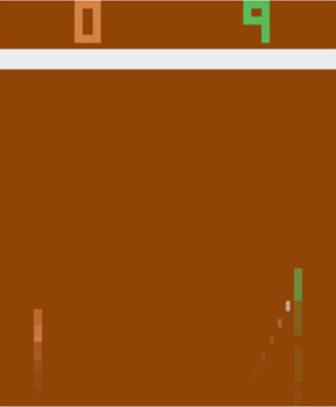
\includegraphics[width=\textwidth]
            {figures/explainability_in_reinforcement_learning/policy_approximation_observation.jpg}
        \caption{}
        \label{fig:policy_approximation_observation}
    \end{subfigure}
    \hspace{0.02\textwidth}
    \begin{subfigure}[b]{0.47\textwidth}
        \centering
        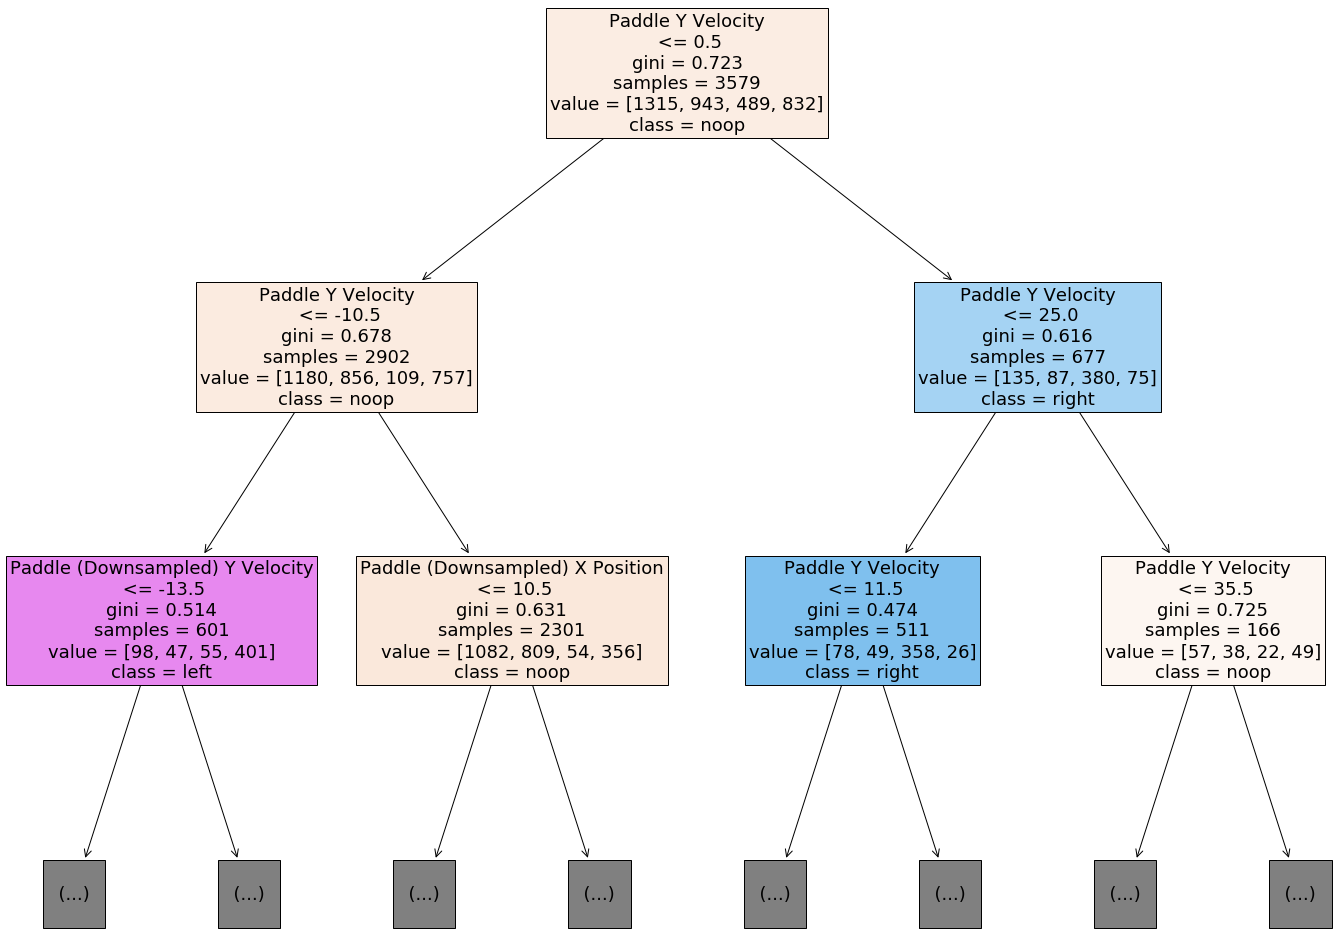
\includegraphics[width=\textwidth]
            {figures/explainability_in_reinforcement_learning/policy_approximation_decision_tree.png}
        \caption{}
        \label{fig:policy_approximation_decision_tree}
    \end{subfigure}
    \caption[Policy approximation via an interpretable model.]{
        Policy approximation via an interpretable model \parencite{sieusahai2021explaining}.
    }
    \label{fig:policy_approximation_example}
\end{figure}


\subsection{Saliency Map}
\label{subsec:saliency_map}

The influence of each part of the input on the action selected by the policy can be visualized using heatmaps (Figure~\ref{fig:saliency_map_heatmap}).
In the \gls{rl} setting, the input corresponds to the observation received by the agent at a given time step.
Heatmaps therefore highlight the regions of the observation that have the greatest influence on the action selection process.
By providing this information, they allow the observer to identify which elements of the environment are considered important by the policy when making a decision.
In Figure~\ref{fig:saliency_map_heatmap}, both panels correspond to the same observation of the Atari game \BreakoutName, with panel~\subref{fig:saliency_map_heatmap_perturbation} obtained by observation perturbation and panel~\subref{fig:saliency_map_heatmap_gradient} by observation gradient analysis.

\begin{figure}[t]
    \centering
    \begin{subfigure}[b]{0.4\textwidth}
        \centering
        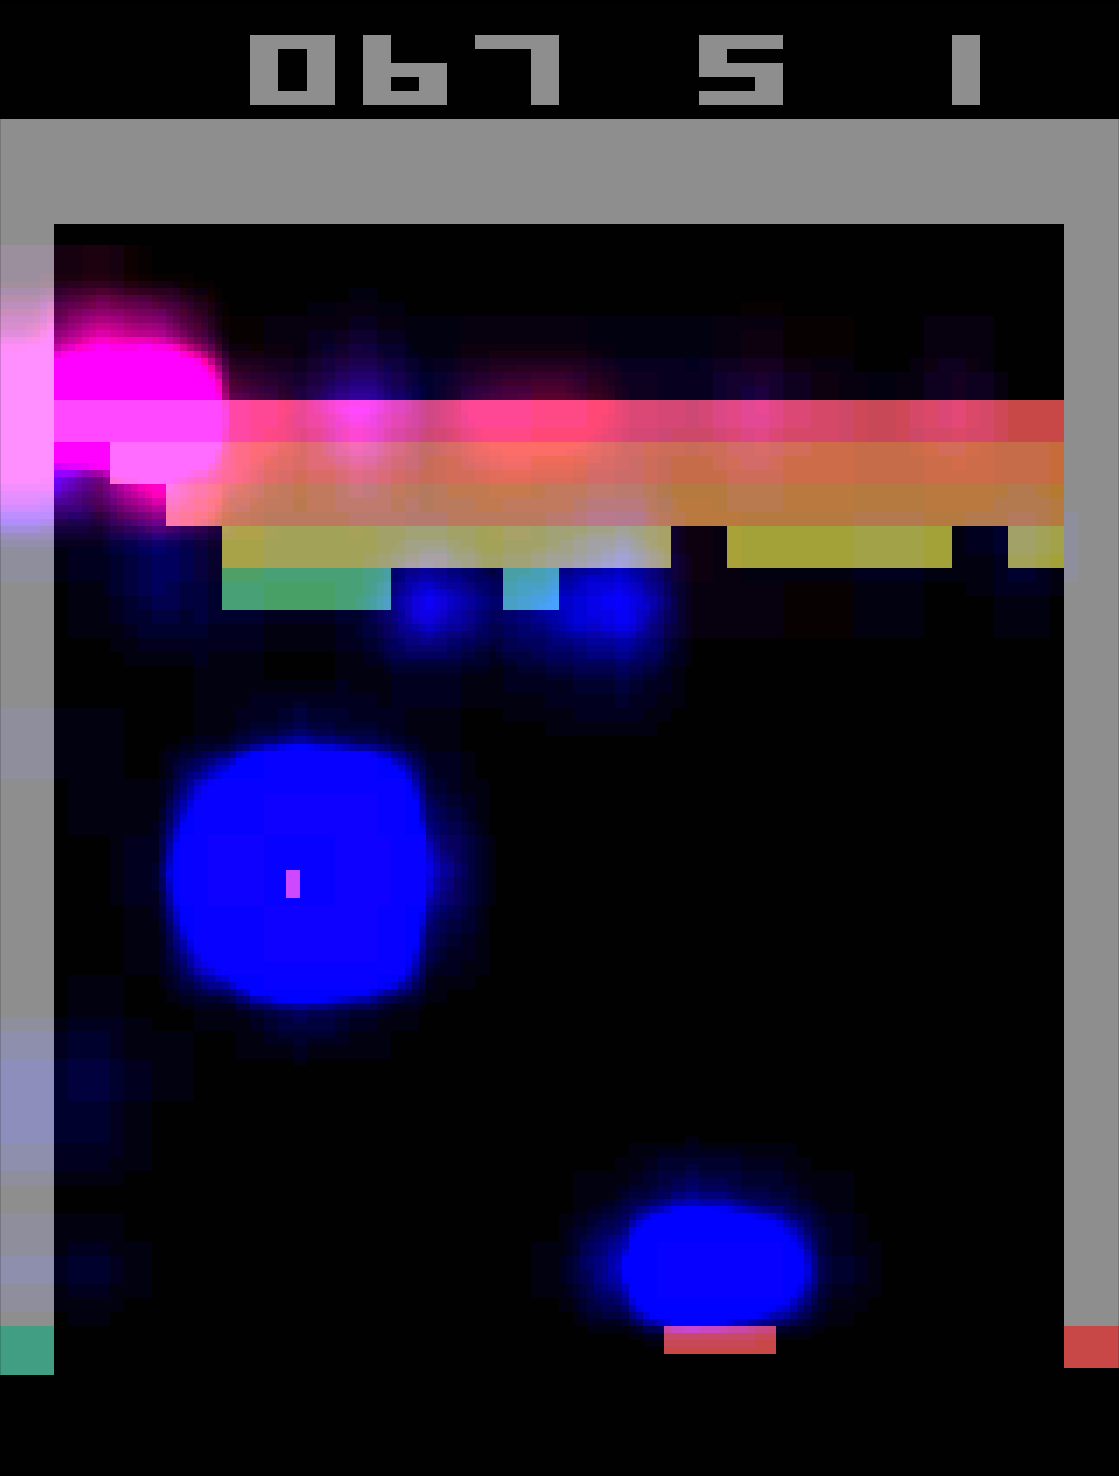
\includegraphics[width=\textwidth]
            {figures/explainability_in_reinforcement_learning/hit_map_1.png}
        \caption{}
        \label{fig:saliency_map_heatmap_perturbation}
    \end{subfigure}
    \hspace{0.02\textwidth}
    \begin{subfigure}[b]{0.4\textwidth}
        \centering
        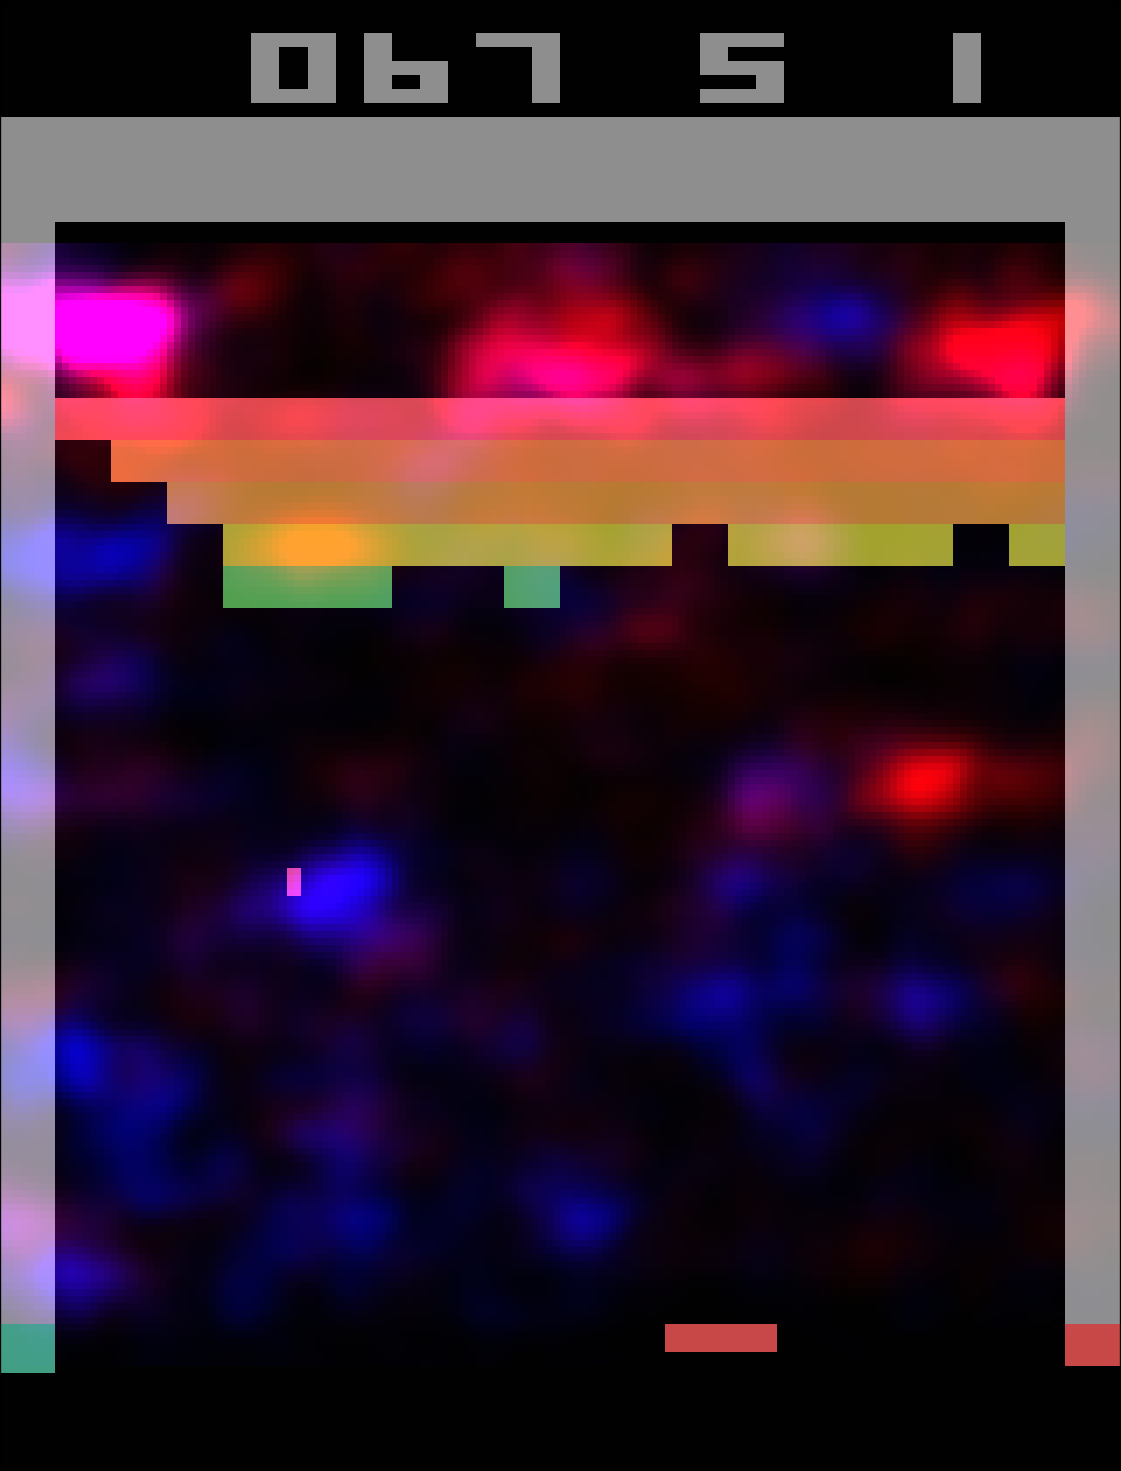
\includegraphics[width=\textwidth]
            {figures/explainability_in_reinforcement_learning/hit_map_2.png}
        \caption{}
        \label{fig:saliency_map_heatmap_gradient}
    \end{subfigure}
    \caption[Saliency heatmaps for \BreakoutName.]{
        Heatmaps for the same observation of the Atari game \BreakoutName \parencite{greydanus2018visualizing}.
    }
    \label{fig:saliency_map_heatmap}
\end{figure}


A limitation of heatmap-based methods is that the resulting explanations are not always directly meaningful to the observer.
As illustrated in Figure~\ref{fig:saliency_map_heatmap_gradient}, interpreting which regions are important often requires human reasoning and involves a degree of subjectivity.
This limitation becomes particularly relevant in \gls{rl}, where the objective is not only to explain a single decision but also to understand the factors influencing a sequence of decisions over time.

Three families of explainability methods can be used to obtain this type of explanation: \textit{observation perturbation}, \textit{observation gradient analysis}, and \textit{attention-based architectures}.

\subsubsection{\textit{Observation Perturbation}}
\label{subsubsec:observation_perturbation}

Perturbation analysis consists in applying various modifications to the observation in order to study their impact on the output of the policy function \parencite{greydanus2018visualizing}.
The greater the variation in the output caused by a perturbation applied to a given component of the input vector, the higher the weight assigned to that component.
The magnitude of the perturbation is measured by computing the distance between the original output and the output obtained from the perturbed input.
Using this set of weights, a \textit{heatmap} is constructed, enabling the observer to visualize which parts of the observation vector are most sensitive in the action-selection process (see Figure~\ref{fig:saliency_map_heatmap_perturbation}).

\subsubsection{\textit{Observation Gradient Analysis}}
\label{subsubsec:observation_gradient_analysis}

Observation gradient analysis refers to a set of methods that require a differentiable policy function in order to extract information from it \parencite{simonyan2014deep, weitkamp2019visual, huber2019enhancing}.
To this end, the gradient of the policy function is computed with respect to all components of the input vector.
For each input component, the resulting gradient provides a weighting that represents its importance in the output of the policy function.
Based on these weightings, a \textit{heatmap} is constructed to allow the observer to visually identify the parts of the input vector that are the most influential in the policy function's output (see Figure~\ref{fig:saliency_map_heatmap_gradient}).

\subsubsection{\textit{Attention-Based Architecture}}
\label{subsubsec:attention_based_architecture}

Attention blocks constitute a \gls{nn} architecture that makes it possible to weight the relative importance of one part of a vector with respect to the other parts of the same vector \parencite{vaswani2017attention}.
These weights are computed as a function of the vector itself and are learned by the \gls{nn} during training.
For a given observation, each component of the observation vector is assigned a scalar value.
It can therefore be assumed that the components associated with the highest weights are the most influential in determining the output \parencite{mott2019towards, itaya2021visual}.

This attention-based \textit{heatmap} is then provided to the observer as the explanation, as illustrated for the Atari game \BreakoutName in Figure~\ref{fig:attention_map_heatmap_clear}, where the highlighted regions are easily interpretable.
However, as shown for \MsPacManName in Figure~\ref{fig:attention_map_heatmap_unclear}, the attention weights are not always concentrated on a small, easily interpretable set of regions, which can make this type of explanation difficult to exploit.

\begin{figure}[t]
    \centering
    \begin{subfigure}[b]{0.4\textwidth}
        \centering
        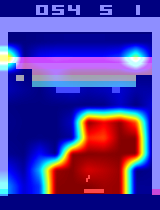
\includegraphics[width=\textwidth]
            {figures/explainability_in_reinforcement_learning/attention_map_1.png}
        \caption{}
        \label{fig:attention_map_heatmap_clear}
    \end{subfigure}
    \hspace{0.02\textwidth}
    \begin{subfigure}[b]{0.4\textwidth}
        \centering
        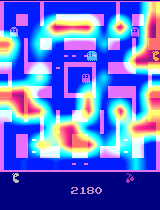
\includegraphics[width=\textwidth]
            {figures/explainability_in_reinforcement_learning/attention_map_2.png}
        \caption{}
        \label{fig:attention_map_heatmap_unclear}
    \end{subfigure}
    \caption[Attention-based heatmaps for \BreakoutName and \MsPacManName.]{
        Attention-based heatmaps for the Atari games \BreakoutName and \MsPacManName \parencite{mott2019towards}.
    }
    \label{fig:attention_map_heatmap}
\end{figure}


\subsection{Counterfactual}
\label{subsec:counterfactual}

A counterfactual explanation is a new observation, close to the original one, that leads the agent to select a different action.
Comparing the two observations reveals which elements of the environment must change for the agent to behave differently, and thus provides insight into its decision-making process.
Unlike the other forms of explanation, this form is currently associated with a single family of methods, based on the \textit{use of the \gls{ls} for counterfactual generation}.

\subsubsection*{\textit{Latent Space Usage for Counterfactual Generation}}
\phantomsection\label{subsubsec:latent_space_counterfactual_generation}

This family of methods uses generative models to build counterfactuals from the \gls{lr} of the observation \parencite{bond2021deep, olson2021counterfactual}.
The observation is encoded into the \gls{ls}, its representation is modified until the agent selects the desired action, and this modified representation is decoded back into a new observation.
Working in the \gls{ls} rather than at the pixel level keeps the counterfactual close to the original state and consistent with the environment.
The fidelity of the generated observations to the real game can then be assessed through user studies \parencite{olson2021counterfactual}.

Figure~\ref{fig:counterfactual_example} illustrates this approach on the Atari game \SpaceInvadersName \parencite{olson2021counterfactual}.
In the original observation (Figure~\ref{fig:counterfactual_example_original}) the agent selects \texttt{LEFT}, whereas in the counterfactual observation (Figure~\ref{fig:counterfactual_example_counterfactual}) it selects \texttt{RIGHT\_FIRE}.
Here, removing an enemy is enough to change the action, which suggests that the position of that enemy influences the agent's decision.
Such observations remain only indicative. Identifying a reliable pattern requires repeating the analysis across many situations.

\begin{figure}[t]
    \centering
    \begin{subfigure}[b]{0.35\textwidth}
        \centering
        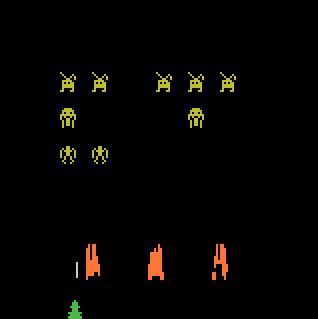
\includegraphics[width=\textwidth]
            {figures/explainability_in_reinforcement_learning/contrefactuel_1.png}
        \caption{}
        \label{fig:counterfactual_example_original}
    \end{subfigure}
    \hspace{0.02\textwidth}
    \begin{subfigure}[b]{0.35\textwidth}
        \centering
        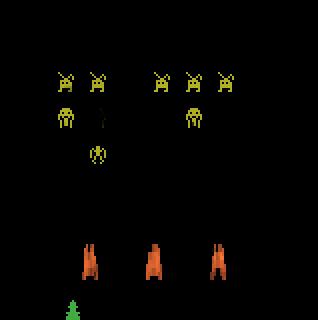
\includegraphics[width=\textwidth]
            {figures/explainability_in_reinforcement_learning/contrefactuel_2.png}
        \caption{}
        \label{fig:counterfactual_example_counterfactual}
    \end{subfigure}
    \caption[Counterfactual explanation for \SpaceInvadersName.]{
        Counterfactual explanation of the agent's behavior for the Atari game \textit{\SpaceInvadersName} \parencite{olson2021counterfactual}.
        Panel~\subref{fig:counterfactual_example_original} shows the original observation and panel~\subref{fig:counterfactual_example_counterfactual} the counterfactual observation produced by a generative model.
    }
    \label{fig:counterfactual_example}
\end{figure}


\subsection{Agent Trajectory}
\label{subsec:agent_trajectory}

Until now, the presented methods have focused on explaining individual decisions made by the agent.
The methods considered from this point on aim to provide insight into the agent's strategy by analyzing its behavior over time.

The most direct approach consists in visualizing agent trajectories, most commonly through complete episodes.
By analyzing these trajectories, the observer can infer the dynamics underlying the agent's behavior and how its decisions evolve through time.
This type of visualization is not specific to \gls{xrl}.
In practice, visualizing agent episodes is a standard step in the development and evaluation of \gls{rl}.
It provides a simple way to verify that the agent behaves as expected and to detect potential implementation errors.

This simple approach can be further enhanced using families of methods such as \textit{hierarchical decomposition} and \textit{extraction via critic analysis}.

\subsubsection{\textit{Extraction via Critic Analysis}}
\label{subsubsec:extraction_via_critic_analysis}

In this family of methods, the predictions of the critic are used to determine which trajectories to present to the observer \parencite{Sequeira_2020}.
A set of states is selected from multiple trajectories.
For a given state, all possible actions are examined.
The state is assigned a value equal to the difference between the critic's prediction for the lowest-valued action and the prediction for the highest-valued action.

Trajectories containing the states with the highest values according to this procedure are then chosen to be presented to the observer.
These trajectories are considered critical moments of the agent and are therefore relevant for analysis.
For this family of methods, the \textit{selected trajectories} represent the interpretable information provided to the observer.

\subsubsection{\textit{Hierarchical Decomposition}}
\label{subsubsec:hierarchical_decomposition}

Hierarchical agents are composed of a set of sub-policies specialized for specific tasks within subsets of the environment's states.
This family of methods distributes the optimization of the reward function across multiple policies.
This decomposition of the policy function can also provide explainability in the agent's strategy \parencite{Beyret_2019}.

If a sub-policy is selected, it indicates that the agent will execute a specialized behavior.
This behavioral specialization provides insight into the strategy the agent employs to maximize the reward function.
The agent's \textit{trajectory}, together with the \textit{sub-policy} selected for each action, is used as interpretable information.

\subsection{Trajectory Prediction}
\label{subsec:trajectory_prediction}

Making predictions about the future of a trajectory allows one to form a representation of what the system expects, based on its training experience.
These predictions are produced using value functions.
Such functions provide insights into the future evolution of the agent's trajectory.
By their nature, this form of explanation informs the observer about the strategy adopted by the agent.

Value functions provide an estimate of the expected cumulative reward from a given state.
Consequently, a value function maps an observation to a scalar value in $\mathbb{R}$.
This aggregated prediction provides limited information about the underlying factors that contribute to this value.
It does not directly reveal which aspects of the task are being optimized or how the predicted return is composed.
Unlike the other forms of explanation, this form is currently associated with a single family of methods, aimed at improving the interpretability of value-based explanations: \textit{critic enrichment}.

\subsubsection*{\textit{Critic Enrichment}}
\phantomsection\label{subsubsec:critic_enrichment}

In order to obtain interpretable information from the predictions of the critic, it is possible to decompose the critic into multiple sub-functions \parencite{juozapaitis2019explainable}.
The reward function is thus decomposed into multiple sub-reward functions, each representing a sub-objective of the task to be accomplished.
Similarly, for each of these sub-reward functions, corresponding sub-critic functions are defined, along with a function that combines their outputs.
During training, the agent selects its actions so as to maximize this combination function of the sub-critics.

Using this approach, for each observation and action, a prediction is obtained regarding the sub-objectives the agent is attempting to maximize, so that the action chosen by the agent reveals which sub-reward it aims to maximize (see Figure~\ref{fig:trajectory_prediction_values}).
This \textit{prediction} is then used as the explanation for the observer.

\begin{figure}[t]
    \centering
    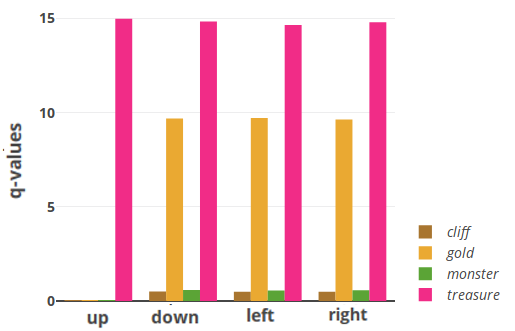
\includegraphics[width=0.8\textwidth]
        {figures/explainability_in_reinforcement_learning/multi_q_values.png}
    \caption[Prediction of sub-rewards as a function of the selected action.]{
        Prediction of sub-rewards as a function of the action selected by the agent for a given state \parencite{juozapaitis2019explainable}.
    }
    \label{fig:trajectory_prediction_values}
\end{figure}


\subsection{Interaction Model}
\label{subsec:interaction_model}

Modeling the interactions between an agent and its environment makes it possible to understand how the agent's decisions are made and what impact they have on the environment.
By incorporating these interactions into an explanatory model, one can better grasp the complex relationships between the agent and its environment, thereby identifying the determining factors in the decision-making process.
By explicitly handling the agent--environment interaction, this type of explanation aims to explain the agent's strategy.

The families of methods used to obtain explanations in the form of agent--environment interactions are: \textit{Bayesian network learning} and \textit{\gls{ls} usage for \gls{mdp} generation}.

\subsubsection{\textit{Bayesian Network Learning}}
\label{subsubsec:bayesian_network_learning}

The evolution of an agent within an environment can be observed as a set of random variables connected through a Bayesian network \parencite{madumal2020explainable}.
Random variables are defined to represent both external aspects (the environment) and internal aspects of the agent (the actions).
By analyzing trajectories, it becomes possible to infer causal relationships among these random variables.

At the end of this process, a weighted causal graph is obtained, which serves as an explanation for the observer, as illustrated for the video game \StarCraftIIName in Figure~\ref{fig:interaction_model_causal_graph}, where nodes represent random variables and edges represent causal relationships between them.
This \textit{Bayesian network}, representing the interactions between the agent and the environment, is then used as the explanation.

\begin{figure}[t]
    \centering
    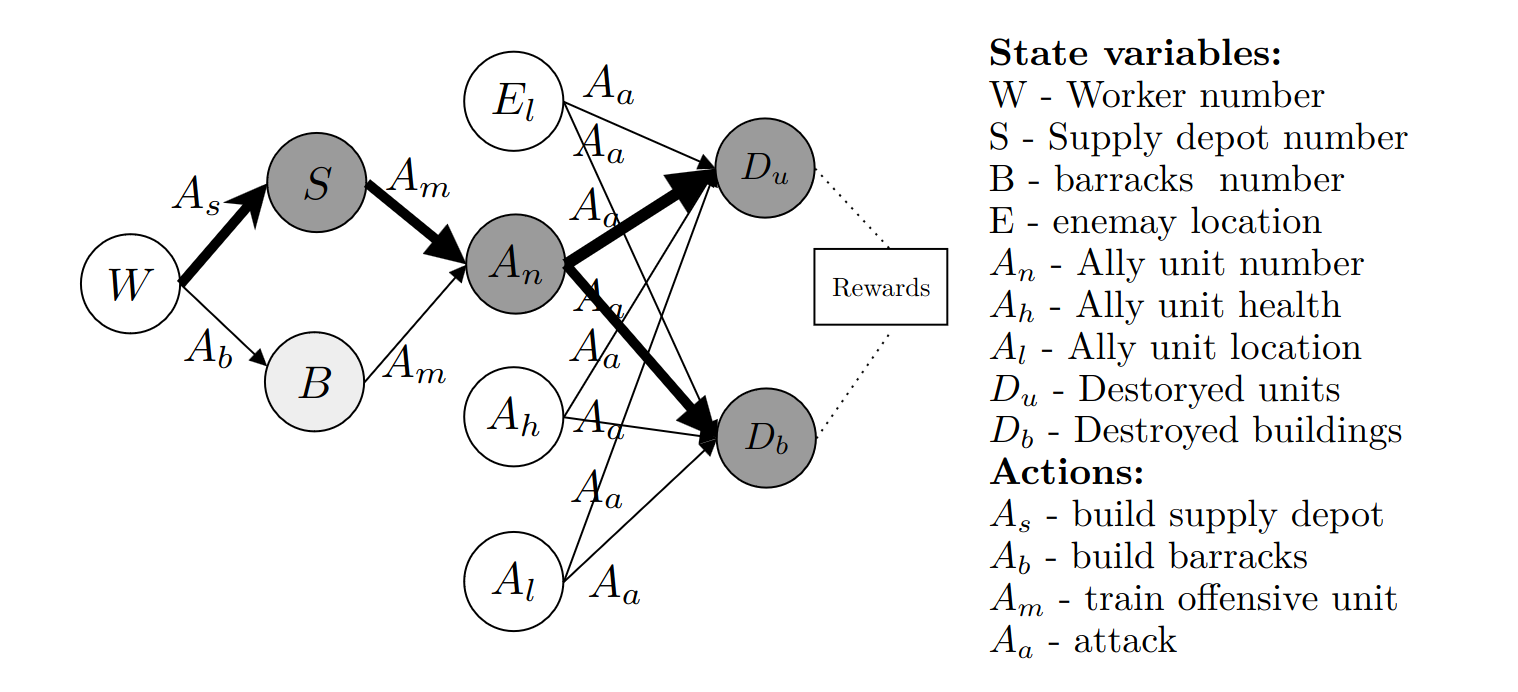
\includegraphics[width=0.9\textwidth]
        {figures/explainability_in_reinforcement_learning/graph_causal.png}
    \caption[Agent--environment interaction model for \StarCraftIIName.]{
        Agent--environment interaction model for the video game \StarCraftIIName \parencite{madumal2020explainable}.
    }
    \label{fig:interaction_model_causal_graph}
\end{figure}


\subsubsection{\textit{Latent Space Usage for Markov Decision Process Generation}}
\label{subsubsec:latent_space_mdp_generation}

As discussed in Chapter~\ref{chap:latent_space_analysis}, each layer of a \gls{nn} can be viewed as a projection from one space to another \parencite{zahavy2017graying}.
As information propagates through successive layers of a \gls{nn}, it becomes increasingly abstract.
It can therefore be assumed that two vectors that are close in this projected space are also close in terms of the agent's perception.

Based on this observation, it is possible to redefine an \gls{mdp} by leveraging the abstract representations produced by the final layers of a \gls{nn}.
Once the new \gls{mdp} has been constructed, a model of the interaction between the agent and its environment is obtained.
This model, represented as a \textit{graph}, is then used as the explanation.

Figure~\ref{fig:latent_space_tsne_example} illustrates this idea using a two-dimensional \textit{t-SNE} projection of the \gls{ls} of the \gls{nn} used to represent the policy.
Each point is colored according to the value function's prediction for the corresponding state, with warmer colors indicating higher predicted values.
An agreement can be observed between the structure of this projected space and the critic's predictions.
States that are assigned similar values by the critic also tend to be located close to one another in the projection.
This agreement makes it possible to manually identify clusters of states, which likely correspond to states that are perceived as similar by the agent.

\begin{figure}[t]
    \centering
    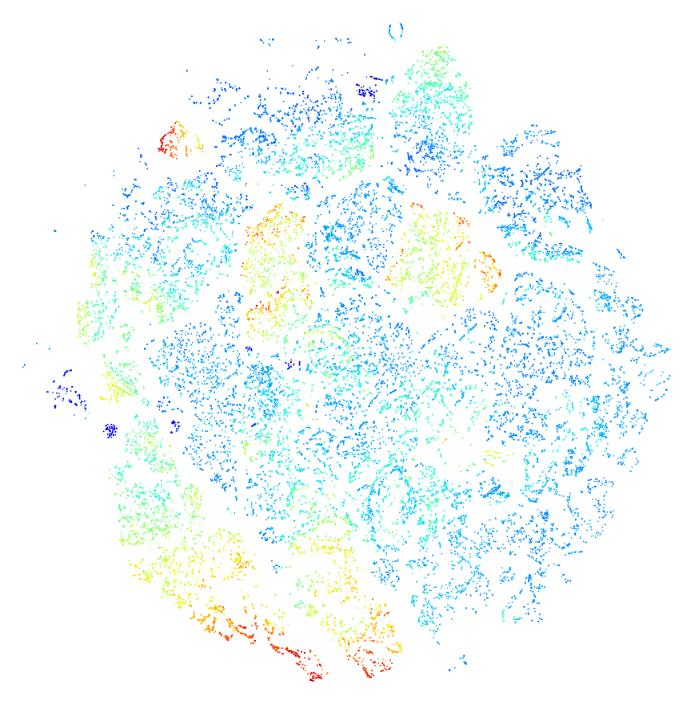
\includegraphics[width=0.8\textwidth]
        {figures/explainability_in_reinforcement_learning/latent_space_tsne_value_function.jpg}
    \caption[\textit{t-SNE} projection of an \glsfmtshort{nn}'s \glsfmtshort{ls}.]{
        \textit{t-SNE} projection of an \glsfmtshort{nn}'s \glsfmtshort{ls}
        \parencite{zahavy2017graying}.
    }
    \label{fig:latent_space_tsne_example}
\end{figure}


\section{Conclusion}
\label{sec:explainability_in_reinforcement_learning_conclusion}

The taxonomy and the state-of-the-art review presented in this chapter make it possible to draw three main observations.

\subsection{Absence of Explanation of the Learning Process}

Regarding the subject of explanation, Table~\ref{tab:taxonomy_methods} shows that none of the reviewed methods addresses the learning process itself.
Such an explanation would concern how the policy is progressively updated throughout training, and why it evolves over successive iterations to converge toward a particular solution.
Several reasons explain this absence.

First, among the different machine learning paradigms, \gls{rl} is arguably the one that would benefit the most from explanations of the learning process.
Unlike supervised or unsupervised learning, it relies on an explicit exploration--exploitation trade-off, making the learning trajectory itself an informative subject of explanation.
However, most \gls{xrl} methods are inherited from the XAI literature, where explanations focus exclusively on the behavior of already-trained models.
This limitation has naturally carried over to \gls{xrl}.

Second, explanations of the learning process have limited value from a practical perspective.
In most real-world applications, practitioners deploy an already-trained agent.
Practitioners are therefore primarily interested in understanding the behavior of the final policy rather than the optimization process that produced it.

Finally, explaining the learning process raises significant methodological challenges.
Training in \gls{rl} can be viewed as the iterative improvement of a policy through repeated interactions with the environment.
In this sense, explaining learning would amount to explaining the evolution of an entire sequence of policies rather than a single one.
Current \gls{xrl} methods still struggle to provide comprehensive explanations of an individual policy, so extending them to a full training trajectory appears considerably more difficult.

\subsection{Lack of Unified Metrics for Explainability}

The diversity of explanation forms identified in this review also reveals another limitation shared by nearly all families of \gls{xrl} methods, which is the absence of reliable metrics for evaluating explainability.
In many studies, explanations are not evaluated with human participants.
Instead, authors focus on technical properties of the proposed method, such as fidelity, sparsity, or computational efficiency.

When human evaluations are conducted, they usually rely on subjective satisfaction questionnaires.
Although useful, self-reported satisfaction remains prone to numerous biases and does not necessarily indicate that the explanation has improved the observer's mental model or understanding of the agent.

This limitation is not specific to \gls{xrl}, it reflects a broader challenge affecting \gls{xai} as a whole.
In our view, this limitation comes from how explainability has developed in artificial intelligence.
Most of the proposed approaches have been developed by the computer science community.
Explainability has consequently often been studied from an algorithmic or mathematical perspective, with less attention given to how humans actually benefit from explanations.

Our definition of explanation explicitly places the observer at the center of the explanatory process.
From this perspective, the value of an explanation should not only depend on its technical properties but also on its ability to improve the observer's understanding.
Addressing this challenge will require stronger interdisciplinary collaboration between computer science and disciplines such as cognitive science, psychology, philosophy, and sociology.
These fields provide the theoretical and experimental tools needed to study human understanding and to develop evaluation protocols that measure the actual effectiveness of explanations.

\subsection{Toward Intrinsic Explainability in Reinforcement Learning}

Our review also suggests that current \gls{xrl} research remains largely dominated by substitutive explainability approaches.
Replacing a deep model with a simpler one therefore risks losing precisely the representational power that makes deep \gls{rl} effective.
For this reason, we argue that a promising direction for \gls{xrl} is to develop explanations directly from the \gls{nn} that forms the agent's policy.
Such approaches aim to analyze the representations learned by the network itself.

Among the methods reviewed, \textit{latent space usage for MDP generation} (Section~\ref{subsubsec:latent_space_mdp_generation}) appears closest to this intrinsic perspective.
However, this approach still relies on a largely manual and qualitative analysis of the \gls{ls}, which limits its reproducibility and its ability to produce systematic explanations.

The next chapter builds upon this idea and proposes a mechanistic \gls{xrl} approach based on \gls{ls} analysis.

\chapter{Clustering Agent Representations}
\label{chap:clustering_agent_representations}

\chapterepigraph{Our analysis shows that there are three kinds of people in the world: those who use $k$-means clustering with $k=3$, and two other types whose qualitative interpretation is unclear.}
{Randall Munroe, \textit{xkcd} no.~2731 (2023)~\parencite{munroe2023kmeans}}

\glsresetall

As discussed in the previous chapter, current explainability methods for \gls{rl} still lack intrinsic approaches capable of explaining the internal mechanisms of deep neural policies.
To the best of our knowledge, only \textcite{zahavy2017graying}, in their paper \citetitle{zahavy2017graying}, have proposed exploiting the \gls{ls} learned by neural policies in order to identify the concepts used by the agent.
Its main idea is to analyze the \glspl{lr} produced by the \gls{nn} and organize them into clusters that correspond to concepts.

While the core idea of this paper is closely aligned with our vision of explainability in \gls{rl}, this approach suffers from two important limitations.
First, the clusters are manually constructed.
Such a procedure heavily depends on the user's expertise and neither guarantees reproducibility or scales.
Second, no evaluation protocol is proposed to assess the quality of the obtained clusters.
Their relevance is essentially determined through visual inspection.

The \gls{car} method proposed in this chapter addresses these two limitations.
First, it automates concept discovery by relying on unsupervised clustering algorithms.
Second, it introduces an objective evaluation metric based on the stability of the extracted representations across independently trained policies.

This chapter is organized as follows:
\begin{itemize}
    \item Section~\ref{sec:clustering_agent_representations_representation_convergence_hypothesis} lays out the theoretical assumptions underlying the proposed \gls{car} method, which we term the \RepresentationConvergenceHypothesisName.
    \item Section~\ref{sec:clustering_agent_representations_latent_clustering_of_surrogate_policies} then details the \gls{car} method itself, covering both the extraction of \glspl{lr} using surrogate policies and the automatic detection of \glspl{cs} through clustering.
    \item Section~\ref{sec:clustering_agent_representations_evaluation_metrics} introduces the metrics we propose for evaluation.
    \item Section~\ref{sec:clustering_agent_representations_conclusion} situates \gls{car} within the broader landscape of \gls{me}.
\end{itemize}

\section{Representation Convergence Hypothesis}
\label{sec:clustering_agent_representations_representation_convergence_hypothesis}

The \gls{car} method relies on an assumption, referred to as the \RepresentationConvergenceHypothesisName.
This hypothesis follows the two assumptions established previously throughout this thesis.

The \MechanisticHypothesisName rejects the notion that deep \glspl{nn} constitute irreducible \enquote{black boxes}.
Adopting a mechanistic perspective, we consider that every process results from a sequence of causal computations.
Although these computations may be complex, they remain explainable through the analysis of the internal mechanisms.

The \ConceptHypothesisName states that \glspl{nn} achieve generalization by learning concepts.
During optimization, the network progressively organizes its \gls{ls} into representations that capture the information required to solve the task.

Following these two hypotheses, it becomes possible to explain a \gls{nn} by studying the organization of its \gls{ls}.
This family of approaches corresponds to \gls{me} (Definition~\ref{def:mechanistic_explainability}).
Since the \gls{car} method is grounded in these two hypotheses, it falls within this field of research.

More specifically, \gls{car} focuses on a specific aspect of \gls{me} known as universality.
Universality refers to the consistency with which a concept is recovered across different models trained on the same task \parencite{templeton2024scaling}.
In the literature, universality is mainly reported as an empirical observation, without an explanation of why it occurs.
In this thesis, we make it a central proposition for explaining \glspl{nn}.
If the same concepts emerge in every model trained on a task, these concepts characterize the task itself, and they can be used to explain the behavior of any of these models.

To provide an explanation for this phenomenon, we developed the \RepresentationConvergenceHypothesisName.
This hypothesis states that, when \glspl{nn} are trained to solve the same task, a set of concepts should systematically emerge because these concepts provide an effective way of representing the problem.
As a result, independently trained models should develop similar concepts in their learned representations.

\begin{hypothesis}{Representation Convergence Hypothesis}{convergence}
For a given task, independently trained \glspl{nn} tend to develop similar sets of concepts because these concepts provide an efficient representation for solving the task.
\end{hypothesis}

The \gls{car} method is designed to investigate the \RepresentationConvergenceHypothesisName by assessing whether it can consistently recover similar concepts across independently trained models.
The hypothesis therefore serves both as the foundation of the method and as the phenomenon it aims to investigate.

If \gls{car} consistently recovers the same set of concepts across different training runs, this set is more likely to reflect invariant properties of the task than model-specific artifacts.
Conversely, the absence of representation convergence would provide evidence against the hypothesis and would also question the validity of the \gls{car} approach.

It is important to clarify that this hypothesis does not imply convergence at the parameter level.
Independently trained models are expected to converge toward different sets of weights.
The proposed hypothesis concerns a abstract level of representation.
We assume that the conceptual organization induced by their \glspl{lr} converges toward an equivalent \gls{cs}, even though the numerical implementation of the networks differ.

The remainder of this chapter develops the methodology used to investigate this hypothesis.
\section{Latent Clustering of Surrogate Policies}
\label{sec:clustering_agent_representations_latent_clustering_of_surrogate_policies}

Following \textcite{zahavy2017graying}, we analyze the \gls{ls} through clustering techniques, placing our approach within the broader field of Deep Clustering.
This design choice is motivated by our rejection of the \SuperpositionHypothesisName and, more generally, of any view that assumes a linearly organized \gls{cs}, as discussed in Section~\ref{sec:latent_space_analysis_clustering}.

The \gls{car} methodology is composed of two main stages.
The first stage trains multiple independent \glspl{nn}, called surrogate policies, which implement the same decision policy.
The second stage clusters their \glspl{lr} in order to identify the underlying conceptual organization.
Once these two stages have been completed, the resulting clustering can be analyzed from two complementary perspectives.
First, the consistency of the resulting clusters across independent training runs can be assessed to determine whether the identified clusters are stable.
Second, the semantic content of the clusters can be examined to determine whether they correspond to meaningful concepts.
Figure~\ref{fig:illustration_method} provides a visual overview of the two stages, from the imitation of the initial policy to the clustering of the surrogate representations.

\begin{figure}[t]
    \centering
    \resizebox{\textwidth}{!}{
    \begin{tikzpicture}
        \node (observation) [minimum height=1.5cm, minimum width=2.5cm, align=center] at (0, 0) {\hl{Observation} \\ \large $o$};

        \node[draw, rectangle, text centered, minimum height=1cm, minimum width=2.5cm, align=center, rounded corners=0.2cm] (policy) at ($(observation) + (3cm, 1.35cm)$) {\scalebox{2}{$\InitialPolicy$}};

        \node[align=center] (policy_text) at ($(policy) + (0, 1cm)$) {Initial Policy};

        \node[draw, rectangle, text centered, minimum height=1cm, minimum width=2.5cm, align=center, rounded corners=0.2cm] (surrogate_policy) at ($(observation) + (3cm, -1.35cm)$) {\scalebox{2}{$\SurrogatePolicy{}$}};

        \node[align=center] (surrogate_policy_text) at ($(surrogate_policy) + (0, 1cm)$) {Surrogate Policy};

        \draw[->] (observation) |- (policy);
        \draw[->] (observation) |- (surrogate_policy);

        \def\B{4};
        \def\S{5};
        \def\Bs{1.0};
        \def\Ss{1.25};
        \def\xmax{\S+3.2*\Ss};

        \begin{axis}[
            name=policy_distribution,
            at={($(policy) + (5cm, 0cm)$)},
            anchor=center,
            every axis plot post/.append style={
                mark=none,domain={-0.05*(\xmax)}:{1.08*\xmax},samples=\numberOfSamplesToPlotCurve,smooth
            },
            xmin=0,
            xmax=\xmax,
            ymin=0,
            ymax={1.1*gauss(\B,\B,\Bs)},
            axis lines=middle,
            axis line style=thick,
            enlargelimits=upper, % extend the axes a bit to the right and top
            ticks=none,
            x=0.5cm,
            y=5cm,
            scale=0.7,
            xlabel={$\ActionSet$},
            xlabel style={at={(axis description cs:0.85,0.2)}, anchor=west},
            % ylabel={probability},
            ylabel style={at={(axis description cs:0,1.02)},anchor=south},
            title={action distribution},
            title style={at={(axis description cs:0.5,-0.15)},anchor=north},
        ]

        % PLOTS
        \addplot[name path=A,thick, mygreen] {gauss(x,\B,\Bs)} node[pos=0.5, above, xshift=-0.8cm, yshift=-0.2cm] {$\InitialPolicy\textcolor{black}{(o)}$};
        \end{axis}

        \begin{axis}[
            name=surrogate_policy_distribution,
            at={($(surrogate_policy) + (5cm, 0cm)$)},
            anchor=center,
            every axis plot post/.append style={
                mark=none,domain={-0.05*(\xmax)}:{1.08*\xmax},samples=\numberOfSamplesToPlotCurve,smooth
            },
            xmin=0,
            xmax=\xmax,
            ymin=0,
            ymax={1.1*gauss(\B,\B,\Bs)},
            axis lines=middle,
            axis line style=thick,
            enlargelimits=upper, % extend the axes a bit to the right and top
            ticks=none,
            x=0.5cm,
            y=5cm,
            scale=0.7,
            xlabel={$\ActionSet$},
            xlabel style={at={(axis description cs:0.85,0.2)}, anchor=west},
            % ylabel={probability},
            ylabel style={at={(axis description cs:0,1.02)},anchor=south},
            title={action distribution},
            title style={at={(axis description cs:0.5,-0.15)},anchor=north},
        ]

        % PLOTS
        \addplot[name path=B,thick,myred] {gauss(x,\S,\Ss)} node[pos=0.5, above, xshift=1.2cm, yshift=-0.3cm] {$\SurrogatePolicy{}\textcolor{black}{(o)}$};
        \end{axis}

        \draw[->] (policy) -- ($(policy_distribution.west) + (-0.2cm, 0)$);
        \draw[->] (surrogate_policy) -- ($(surrogate_policy_distribution.west) + (-0.2cm, 0)$);

        \begin{axis}[
            name=distribution_match,
            at={(13.5cm, 0cm)},
            anchor=center,
            every axis plot post/.append style={
                mark=none,domain={-0.05*(\xmax)}:{1.08*\xmax},samples=\numberOfSamplesToPlotCurve,smooth
            },
            xmin=0,
            xmax=\xmax,
            ymin=0,
            ymax={1.1*gauss(\B,\B,\Bs)},
            axis lines=middle,
            axis line style=thick,
            enlargelimits=upper, % extend the axes a bit to the right and top
            ticks=none,
            x=0.5cm,
            y=5cm,
            scale=0.8,
            xlabel={$\ActionSet$},
            xlabel style={at={(axis description cs:0.85,0.2)}, anchor=west},
            % ylabel={probability},
            ylabel style={at={(axis description cs:0,1.02)},anchor=south},
            title={\shortstack{difference between \\[0.08cm] distributions}},
            title style={at={(axis description cs:0.5,-0.15)},anchor=north},
        ]

        % PLOTS
        \addplot[name path=A,thick,mygreen] {gauss(x,\B,\Bs)} node[pos=0.5, above, xshift=-0.8cm, yshift=-0.2cm] {$\InitialPolicy\textcolor{black}{(o)}$};
        \addplot[name path=B,thick,myred] {gauss(x,\S,\Ss)} node[pos=0.5, above, xshift=1.2cm, yshift=-0.3cm] {$\SurrogatePolicy{}\textcolor{black}{(o)}$};

        \addplot[opacity=0.2] fill between[of=A and B, soft clip={domain=0:15}];
        \end{axis}

        \node[align=center] at ($(distribution_match.north) + (0, 1.25cm)$) {$\SurrogatePolicy{}$ is trained to be as close as \\ possible of $\InitialPolicy$ for all $o$ in order \\ to reproduce its behavior.};

        \draw[->] ($(policy_distribution.east) + (0.2cm, 0)$) -- ($(policy_distribution.east) + (0.5cm, 0)$) |- ($(distribution_match.west) + (-0.2cm, 0)$);
        \draw[->] ($(surrogate_policy_distribution.east) + (0.2cm, 0)$) -- ($(surrogate_policy_distribution.east) + (0.5cm, 0)$) |- ($(distribution_match.west) + (-0.2cm, 0)$);

        \begin{scope}[xshift=8cm, yshift=-5cm, scale=0.8, transform shape]
            \node[draw, minimum width=4cm, minimum height=4cm] (box_2) at (0, 0) {};

            \begin{scope}
                \clip (box_2.south west) rectangle (box_2.north east);

                \node[draw, dashed, minimum width=1.5cm, circle, minimum height=1.5cm] (circle_1) at (-1.25cm, -1.25cm) {};

                \node[draw, dashed, minimum width=1.5cm, circle, minimum height=1.5cm] (circle_2) at (0cm, 1.75cm) {};

                \node[draw, dashed, minimum width=1.5cm, circle, minimum height=1.5cm] (circle_3) at (1.75cm, 0cm) {};
            \end{scope}

            \foreach \x/\y in {
                -1.5/-0.75,
                -1.25/-1.5,
                -1/-1.75,
                -1.75/-1.25,
                -0.75/-1.25,
                -1/-1,
                0.5/1.5,
                -0.25/1.25,
                0.0/1.50,
                -0.5/1.5,
                0/1.25,
                1.5/-0.5,
                1.5/0.5,
                1.25/0.25,
                1.5/0,
                1.25/-0.25
            }
            {
                \node[] (p1) at (\x cm,\y cm) {\textcolor{myblue}{$\times$}};
            }
        \end{scope}
        \draw[->, dashed, preaction={draw=white,line width=6pt}] (surrogate_policy) |- ($(box_2.west) + (-0.2cm, 0)$);

        \node[draw, rectangle, text centered, align=center, dashed, fill=white, inner sep=1.5mm] at ($(surrogate_policy) - (0, 2.0cm)$) {Projection obtained through \\ the function $\SurrogateEncoder$, which is \\ a subcomponent of $\SurrogatePolicy{}$.};

        \node[align=center] at ($(box_2.east) + (2.75cm, 0)$) {Once $\SurrogatePolicy{}$ is trained,\\ observations are projected into $\LatentSet{}$,\\ clustered automatically,\\ and interpreted for semantics.};

        \node[align=center] at ($(box_2.south) + (0, -0.3cm)$) {\gls{ls} $\LatentSet{}$ of $\SurrogatePolicy{}$};
    \end{tikzpicture}
    }
    \caption{Illustration of the \methodName method.}
    \label{fig:illustration_method}
\end{figure}


This section is organized into three parts.
The first explains why multiple surrogate policies are used to study the stability of the representations.
The second describes how these policies are trained to match the initial policy as closely as possible.
The third presents how their \glspl{lr} are clustered to identify the \glspl{cs}.

\subsection{Multiple Surrogate Policies}

The \gls{car} method was developed to test the \RepresentationConvergenceHypothesisName.
This requires training several \glspl{nn} independently and comparing their \glspl{lr}.
Consistent similarities in the resulting \glspl{cs} would provide empirical support for this hypothesis.

In supervised learning, this protocol is straightforward since several models can be independently trained on the same target function.
\gls{rl} introduces an additional difficulty.
Because of stochastic exploration, independently trained agents are not guaranteed to converge toward the same policy.
Even if they achieve comparable performance, they may solve the task using different strategies.
This makes it difficult to determine whether differences in the \gls{ls} result from different representations of the same strategy or from differences in the learned strategies themselves.

To overcome this limitation, we consider an already trained initial policy.
This policy is then used as a target for imitation learning \parencite{pmlr-v15-ross11a}.
In this process, several surrogate \glspl{nn} are independently trained in a supervised manner to reproduce the behavior of the same agent.
This allows us to investigate whether \glspl{nn} that learn equivalent policies also develop similar conceptual organizations.

It is important to emphasize that the use of surrogate policies does not make \gls{car} a surrogate explainability method, as defined in Subsection~\ref{subsec:explainable_artificial_intelligence}.
The surrogate policies remain deep \glspl{nn}.
Their role is not to simplify the decision process but to provide multiple independent realizations of the same policy function, enabling the study of representation convergence.

\subsection{Training Surrogate Policies}

Throughout the remainder of this thesis, the initial policy we aim to explain is denoted as $\InitialPolicy$.
This initial policy is obtained without imposing any constraints on its origin.
It may result from classical or deep reinforcement learning \parencite{sutton2018reinforcement}, alpha-beta algorithm \parencite{knuth1975analysis}, or even from demonstrations provided by humans \parencite{pmlr-v9-ross10a}.
The crucial requirement is the availability of a dataset containing a sufficient number of projections from the observation space $\ObsSet$ to the action space $\ActionSet$ induced by $\InitialPolicy$ to train a \gls{nn}.

The replicated policies are referred to as surrogate policies.
To assess the stability of the learned representations, $n$ surrogate policies are trained independently, denoted by $\SurrogatePolicy{1}, \dots, \SurrogatePolicy{n}$.
All surrogate policies share the same architecture.
It consists of a \gls{nn} with two components, an encoder $\SurrogateEncoder$ and a decoder $\Decoder$, highlighted by the blue and black dashed rectangles, respectively, in Figure~\ref{fig:surrogate_policy_architecture}.
The encoder maps the observation $o$ to the embedding, and the decoder reconstructs the parameters of the action distribution from this embedding.
For a given surrogate policy $\SurrogatePolicy{i}$, parameterized by $\params_i$, its encoder and decoder are written $\SurrogateEncoder[i]$ and $\Decoder[i]$.

\begin{figure}[t]
    \centering
    \resizebox{\textwidth}{!}{
    \begin{tikzpicture}[x=3cm,y=1cm]
    \large
    \message{^^JDeep convolution neural network}
    \readlist\Nnod{4,5,6,5,3}
    \def\nstyle{1}
    \tikzset{
    node 1/.style={thick,circle,draw,minimum size=18,inner sep=0.5,outer sep=0.6},
    }

    \message{^^J  Layer}
    \foreachitem \N \in \Nnod{
        \def\lay{\Ncnt}
        \pgfmathsetmacro\prev{int(\Ncnt-1)}
        \message{\lay,}
        \foreach \i [evaluate={\y=\N/2-\i+0.5; \x=\lay; \n=\nstyle;}] in {1,...,\N}{ % loop over nodes
            \ifboolexpr{test {\ifnumcomp{\lay}{=}{3}}}
            {
                \node[node \n,outer sep=0.6] (N\lay-\i) at (\x,\y) {\textcolor{myblue}{$h^{(\lay)}_{\i}$}};
            }
            {
                \node[node \n,outer sep=0.6] (N\lay-\i) at (\x,\y) {};
            }

            \ifnum\lay>1
            \foreach \j in {1,...,\Nnod[\prev]}{ % loop over nodes in previous layer
                \draw[] (N\prev-\j) -- (N\lay-\i);
            }
            \fi
        }
    }

    \coordinate (policy_top_margin) at ($(N3-1) + (0, 1.3cm)$);
    \node[draw, rectangle, fit=(N1-1)(N3-6)(N5-1)(policy_top_margin), inner sep=0.25cm, dashed, rounded corners=0.3cm, color=myred] (policy) {};
      \node[] (policy_label) at ($(policy.north) + (0, 0.5cm)$) {\scalebox{2.5}{$\SurrogatePolicy{}$}};

    % Encoder box: encloses the layers up to and including the embedding
    \node[draw, dashed, rounded corners=0.15cm, color=myblue, fit=(N1-1)(N1-4)(N3-1)(N3-6), inner sep=0.15cm] (encoder_box) {};
    \node[align=center] (encoder_label) at ($(encoder_box.north) + (0, 0.5cm)$) {\scalebox{1.5}{$\SurrogateEncoder$}};

    % Decoder box: encloses the embedding and the layers up to the output
    \node[draw, dashed, rounded corners=0.15cm, color=black, fit=(N3-1)(N3-6)(N5-1), inner sep=0.15cm] (decoder_box) {};
    \node[align=center] (decoder_label) at ($(decoder_box.north) + (0, 0.5cm)$) {\scalebox{1.5}{$f_{dec}$}};

    % Observation
    \node[minimum height=1cm, minimum width=1cm] (observation_1) at ($(N1-1) + (-1.75cm, 0)$) {\scalebox{1.25}{$o_1$}};
    \node[minimum height=1cm, minimum width=1cm] (observation_2) at ($(N1-2) + (-1.75cm, 0)$) {\scalebox{1.25}{$o_2$}};
    \node[minimum height=1cm, minimum width=1cm] (observation_3) at ($(N1-3) + (-1.75cm, 0)$) {\scalebox{1.25}{$o_3$}};
    \node[minimum height=1cm, minimum width=1cm] (observation_4) at ($(N1-4) + (-1.75cm, 0)$) {\scalebox{1.25}{$o_4$}};

    \node[minimum height=1cm, minimum width=1cm, align=center] (observation_label) at ($(observation_1) + (0, 1.25cm)$) {\hl{Observation}};

    \draw[thick] (observation_1.north east) -- ($(observation_1.north east) + (-0.1cm, 0)$);
    \draw[thick] (observation_1.north east) -- (observation_4.south east);
    \draw[thick] (observation_4.south east) -- ($(observation_4.south east) + (-0.1cm, 0)$);

    \draw[thick] (observation_1.north west) -- ($(observation_1.north west) + (0.1cm, 0)$);
    \draw[thick] (observation_1.north west) -- (observation_4.south west);
    \draw[thick] (observation_4.south west) -- ($(observation_4.south west) + (0.1cm, 0)$);

    \draw[->] ($(observation_1.east) + (-0.15cm, 0)$) -- ($(N1-1.west) + (-0.0cm, 0)$);
    \draw[->] ($(observation_2.east) + (-0.15cm, 0)$) -- ($(N1-2.west) + (-0.0cm, 0)$);
    \draw[->] ($(observation_3.east) + (-0.15cm, 0)$) -- ($(N1-3.west) + (-0.0cm, 0)$);
    \draw[->] ($(observation_4.east) + (-0.15cm, 0)$) -- ($(N1-4.west) + (-0.0cm, 0)$);

    % Distribution
    \node[minimum height=1cm, minimum width=1cm] (distribution_1) at ($(N5-1) + (1.75cm, 0)$) {\scalebox{1.25}{$\ell_1$}};
    \node[minimum height=1cm, minimum width=1cm] (distribution_2) at ($(N5-2) + (1.75cm, 0)$) {\scalebox{1.25}{$\ell_2$}};
    \node[minimum height=1cm, minimum width=1cm] (distribution_3) at ($(N5-3) + (1.75cm, 0)$) {\scalebox{1.25}{$\ell_3$}};

    \draw[thick] (distribution_1.north east) -- ($(distribution_1.north east) + (-0.1cm, 0)$);
    \draw[thick] (distribution_1.north east) -- (distribution_3.south east);
    \draw[thick] (distribution_3.south east) -- ($(distribution_3.south east) + (-0.1cm, 0)$);

    \draw[thick] (distribution_1.north west) -- ($(distribution_1.north west) + (0.1cm, 0)$);
    \draw[thick] (distribution_1.north west) -- (distribution_3.south west);
    \draw[thick] (distribution_3.south west) -- ($(distribution_3.south west) + (0.1cm, 0)$);

    \draw[->] ($(N5-1.east) + (0.0cm, 0)$) -- ($(distribution_1.west) + (0.2cm, 0)$);
    \draw[->] ($(N5-2.east) + (0.0cm, 0)$) -- ($(distribution_2.west) + (0.2cm, 0)$);
    \draw[->] ($(N5-3.east) + (0.0cm, 0)$) -- ($(distribution_3.west) + (0.2cm, 0)$);

    \node[minimum height=1cm, minimum width=1cm, align=center] (distribution_label) at ($(distribution_1) + (0, 1.5cm)$) {Parameters \\ for the \\ \hl{Distribution}};

    % Embedding
    \node[align=center] (embedding_label) at ($(N3-6) + (0cm, -2cm)$) {\hl{Embedding}};

    \draw[thick, dashed, ->] ($(N3-6) + (0cm, -0.5cm)$) -- ($(embedding_label) + (0cm, 0.5cm)$);

    \node[] (embedding) at ($(embedding_label) + (0, -2cm)$) {
        $\begin{bmatrix}
            \textcolor{myblue}{h^{(3)}_{1}} \\
            \textcolor{myblue}{h^{(3)}_{2}} \\
            \textcolor{myblue}{h^{(3)}_{3}} \\
            \textcolor{myblue}{h^{(3)}_{4}} \\
            \textcolor{myblue}{h^{(3)}_{5}} \\
            \textcolor{myblue}{h^{(3)}_{6}}
        \end{bmatrix}$
    };

    \end{tikzpicture}
}
    \caption{Example of a surrogate policy architecture $\SurrogatePolicy{}$.}
    \label{fig:surrogate_policy_architecture}
\end{figure}


To train each surrogate policy $\SurrogatePolicy{i}$ to accurately replicate the action distribution, we define a loss function $\mathcal{L}$ optimized via gradient descent as introduced in Section~\ref{sec:deep_learning_learning}.
This loss, defined in Equation~\eqref{eq:car_loss}, is computed as the \gls{mse} between the parameters of the action distributions, obtained by applying the function $\logits$, which maps a distribution to its parameters (the logits).
In practice, this function $\logits$ does not need to be explicitly defined, as neural policies directly output the parameters of the action distribution.
Each surrogate policy $\SurrogatePolicy{i}$ is thus trained by solving:
\begin{align}
    \min_{\params_i} \sum_{o \in \ObsSet}
    \MSE\Big(
        \logits\big(\InitialPolicy\left(o\right)\big),
        \logits\big(\SurrogatePolicy{i}\left(o\right)\big)
    \Big).
    \label{eq:car_loss}
\end{align}

\subsection{Cluster Extraction}

Once the surrogate policies are trained, their encoders are used to generate a point cloud from a set of observations.
This point cloud provides a sample of the \gls{ls} to be analyzed.
The proposed \gls{car} method adopts the deep clustering approach introduced in Section~\ref{sec:latent_space_analysis_clustering}.
Under this approach, conceptually similar observations are expected to produce nearby \glspl{lr}.
A \gls{cs} can therefore be viewed as a region of the \gls{ls} containing related \glspl{lr}.
To identify these regions, a clustering algorithm is applied to the point cloud.

The clustering is performed independently for each surrogate policy.
For a surrogate policy $\SurrogatePolicy{i}$, applying its encoder $\SurrogateEncoder[i]$ to a subset of observations $\ObsData \subseteq \ObsSet$ yields the set of embeddings $\LatentSet{i}$.
A clustering function $\ClusteringFunction$ then partitions the point cloud $\LatentSet{i}$ into groups of nearby \glspl{lr}, assigning each observation a cluster label and yielding the partition $\mathcal{C}_{i}$.
The same observation set $\ObsData$ is used for every surrogate policy, so that the partitions $\mathcal{C}_{1}, \dots, \mathcal{C}_{n}$ are defined over the same observations and can be compared.
This comparison is the basis of the evaluation introduced in the following section.

Algorithm~\ref{alg:car} states the complete \gls{car} procedure, whose lines map directly onto the stages described above.
Lines~\ref{alg:car:dataset}--\ref{alg:car:loss} prepare the imitation of the initial policy.
They build the training dataset by pairing each observation with the parameters of the action distribution produced by $\InitialPolicy$, and define the \gls{mse} loss of Equation~\eqref{eq:car_loss}.
Lines~\ref{alg:car:train_loop}--\ref{alg:car:sgd} correspond to the first stage, in which each of the $n$ surrogate policies is initialized randomly and trained independently by stochastic gradient descent.
Lines~\ref{alg:car:cluster_loop}--\ref{alg:car:clust} correspond to the second stage.
The encoder of each surrogate policy embeds the shared observation set $\ObsData$ (Line~\ref{alg:car:embed}), and the resulting point cloud is partitioned by $\ClusteringFunction$ (Line~\ref{alg:car:clust}).
Finally, Line~\ref{alg:car:return} returns the surrogate policies together with their partitions, which are the inputs of the evaluation.

\begin{algorithm}[t]
\caption{\glsfmtlong{car} (\glsfmtshort{car})}
\label{alg:car}

\Input{
\\
Initial policy $\InitialPolicy$\\
Observation dataset $\ObsData$\\
Number of surrogate policies $n$\\
Surrogate policy architecture $\SurrogatePolicy{}$ (encoder $\SurrogateEncoder$, decoder $\Decoder$)\\
Learning rate $\eta$\\
Clustering function $\ClusteringFunction$
}

\Output{
\\
Trained surrogate policies $\SurrogatePolicy{1}, \dots, \SurrogatePolicy{n}$\\
Clusterings $\mathcal{C}_{1}, \dots, \mathcal{C}_{n}$
}

\AlgoRule

\tcp{Behavioral cloning dataset built from the target policy $\InitialPolicy$}
$\mathcal{D} \leftarrow \big\{ \big(o, \logits(\InitialPolicy(o))\big) \mid o \in \ObsData \big\}$\nllabel{alg:car:dataset}\;

\BlankLine
\tcp{MSE loss between action-distribution parameters, as defined in Equation~\eqref{eq:car_loss}}
$\mathcal{L} \leftarrow$ \gls{mse}\nllabel{alg:car:loss}\;

\BlankLine
\tcp{Independently train $n$ surrogate policies by behavioral cloning}
\For{$i = 1, \dots, n$\nllabel{alg:car:train_loop}}{
    Initialize $\params_i$ randomly\;

    \BlankLine
    \tcp{Behavioral cloning of $\InitialPolicy$ via SGD, see Algorithm~\ref{alg:stochastic_gradient_descent}}
    $\params_i \leftarrow$ \FnSGD{$\mathcal{D}, \SurrogatePolicy{}, \mathcal{L}, \eta, \params_i$}\nllabel{alg:car:sgd}\;
}

\BlankLine
\tcp{Cluster the latent representations of each surrogate policy}
\For{$i = 1, \dots, n$\nllabel{alg:car:cluster_loop}}{
    \tcp{Embeddings produced by the encoder of $\SurrogatePolicy{i}$}
    $\LatentSet{i} \leftarrow \big\{ \SurrogateEncoder[i](o) \mid o \in \ObsData \big\}$\nllabel{alg:car:embed}\;

    \BlankLine
    \tcp{Partition of the embedded observations into clusters}
    $\mathcal{C}_{i} \leftarrow \ClusteringFunction(\LatentSet{i})$\nllabel{alg:car:clust}\;
}

\BlankLine
\Return{\nllabel{alg:car:return}$\big(\SurrogatePolicy{1}, \dots, \SurrogatePolicy{n}\big), \big(\mathcal{C}_{1}, \dots, \mathcal{C}_{n}\big)$}

\end{algorithm}


Two choices govern this analysis without being part of the clustering algorithm itself.
The first is the choice of layer used to extract the representations.
Each hidden layer defines its own \gls{ls}, reflecting the information represented at that stage of the network.
\gls{car} can therefore be applied to the \glspl{lr} extracted from any layer.
This allows the conceptual organization of the policy to be examined at different levels of the network.

The second is the number of clusters.
\gls{car} does not assume that a task admits a single correct number of concepts.
This choice instead determines the granularity at which the conceptual organization is examined.
A small number reveals broad, strategic concepts, while a larger number reveals finer, tactical ones.
The influence of both choices is studied in Chapter~\ref{chap:experiments}.

Figure~\ref{fig:space_invaders_projection} shows the outcome of this procedure for a surrogate policy trained on \SpaceInvadersName, using five clusters.
The clusters are computed in the original high-dimensional \gls{ls}.
The point cloud is a two-dimensional projection used only for visualization.
Each cluster gathers observations that correspond to a distinct, interpretable stage of a game:
\begin{itemize}
    \item \textbf{Cluster 1:} The start of a game, with few or no invaders neutralized.
    \item \textbf{Cluster 2:} The right-hand group of invaders eliminated.
    \item \textbf{Cluster 3:} The pursuit of the bonus saucer.
    \item \textbf{Cluster 4:} The end of a game, with a few fast invaders close to the ground.
    \item \textbf{Cluster 5:} The middle of a game, with the invaders descending but already thinned out.
\end{itemize}

\NewDocumentCommand{\insertImageWithLine}{m m m m m}{
    \node[draw=#5, line width=6pt, inner sep=0] (#1) at (#2,#3) {
        \includegraphics[width=2.5cm]{#4}
    };
}

\definecolor{custom_blue}{HTML}{40568d}
\definecolor{custom_yellow}{HTML}{fee826}
\definecolor{custom_purple}{HTML}{440053}
\definecolor{custom_light_green}{HTML}{5eca61}
\definecolor{custom_dark_green}{HTML}{22928d}

\begin{figure}[t]
    \centering

    % --- Point cloud + cluster thumbnails, resized to \textwidth independently. ---
    % No longer tied to the legend's own scale factor, so it uses the full page
    % width on its own instead of being capped by the (wider) legend drawing.
    \resizebox{\textwidth}{!}{
        \begin{tikzpicture}
            \begin{pgfonlayer}{background}
                \node[anchor=south west,inner sep=0] (image) at (0,0) {
                    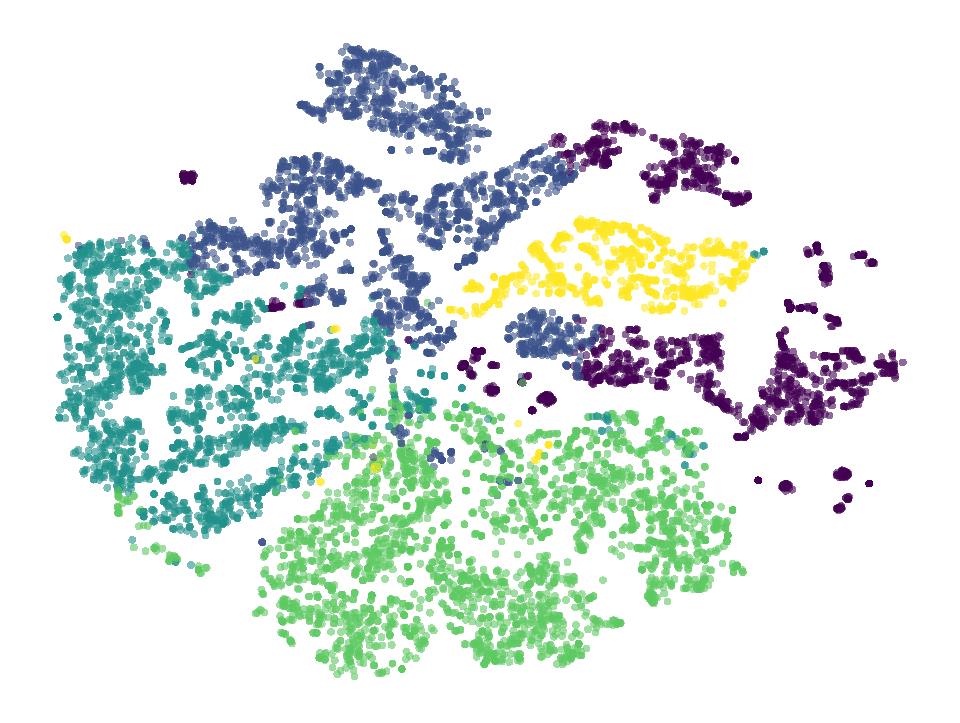
\includegraphics[]{figures/clustering_agent_representations/resources/projection_2d.pdf}
                };
            \end{pgfonlayer}

            \begin{scope}[x={(image.south east)},y={(image.north west)}]
                \node[circle, draw, inner sep=0.2cm, fill=white] (cluster_1) at (0.4,0.75) {\textbf{1}};
                \insertImageWithLine{image_1}{0.17}{0.85}{figures/clustering_agent_representations/pictures/space_invaders/5_clusters/early_game/image_1.png}{custom_blue}
                \insertImageWithLine{image_1}{0.35}{0.95}{figures/clustering_agent_representations/pictures/space_invaders/5_clusters/early_game/image_2.png}{custom_blue}

                \node[circle, draw, inner sep=0.2cm, fill=white] (cluster_2) at (0.65,0.63) {\textbf{2}};
                \insertImageWithLine{image_1}{0.57}{0.85}{figures/clustering_agent_representations/pictures/space_invaders/5_clusters/finish_right_group/image_1.png}{custom_yellow}
                \insertImageWithLine{image_1}{0.75}{0.85}{figures/clustering_agent_representations/pictures/space_invaders/5_clusters/finish_right_group/image_2.png}{custom_yellow}

                \node[circle, draw, inner sep=0.2cm, fill=white] (cluster_3) at (0.775,0.50) {\textbf{3}};
                \insertImageWithLine{image_1}{0.9}{0.55}{figures/clustering_agent_representations/pictures/space_invaders/5_clusters/catch_flying_saucer/image_1.png}{custom_purple}
                \insertImageWithLine{image_1}{0.85}{0.25}{figures/clustering_agent_representations/pictures/space_invaders/5_clusters/catch_flying_saucer/image_2.png}{custom_purple}

                \node[circle, draw, inner sep=0.2cm, fill=white] (cluster_4) at (0.525,0.25) {\textbf{4}};
                \insertImageWithLine{image_1}{0.65}{0.125}{figures/clustering_agent_representations/pictures/space_invaders/5_clusters/late_game/image_1.png}{custom_light_green}
                \insertImageWithLine{image_1}{0.40}{0.125}{figures/clustering_agent_representations/pictures/space_invaders/5_clusters/late_game/image_2.png}{custom_light_green}

                \node[circle, draw, inner sep=0.2cm, fill=white] (cluster_5) at (0.25,0.45) {\textbf{5}};
                \insertImageWithLine{image_1}{0.075}{0.50}{figures/clustering_agent_representations/pictures/space_invaders/5_clusters/mid_game/image_1.png}{custom_dark_green}
                \insertImageWithLine{image_1}{0.175}{0.20}{figures/clustering_agent_representations/pictures/space_invaders/5_clusters/mid_game/image_2.png}{custom_dark_green}
            \end{scope}
        \end{tikzpicture}
    }

    \vspace{0.2cm}

    % --- Legend, resized to \textwidth on its own. ---
    % Spacing between and within the two columns is untouched: same offsets, same
    % single-line entries, only the reference point moved from (image.south) to (0,0).
    % Since this legend was already the widest element in the original combined
    % figure, resizing it alone to \textwidth reproduces its original on-page size.
    \resizebox{\textwidth}{!}{
        \begin{tikzpicture}
            \node (element_1) at (-7cm, -1.5cm) {:};
            \node[anchor=west] (element_1_text) at ($(element_1) + (0.1cm, 0cm)$) {Projection of observations into the latent space.};
            \node[anchor=east] (element_1_symbol) at ($(element_1) + (-0.1cm, 0cm)$) {
                \tikz \fill[custom_blue] (0,0) circle (3pt);
                \tikz \fill[custom_yellow] (0,0) circle (3pt);
                \tikz \fill[custom_purple] (0,0) circle (3pt);
                \tikz \fill[custom_light_green] (0,0) circle (3pt);
                \tikz \fill[custom_dark_green] (0,0) circle (3pt);
                \hspace{0.02cm}
            };

            \node (element_2) at ($(element_1) + (0cm, -0.35cm)$) {:};
            \node[anchor=west] (element_2_text) at ($(element_2) + (0.1cm, 0cm)$) {Corresponding observations to the clusters.};
            \node[anchor=east] (element_2_symbol) at ($(element_2) + (-0.1cm, 0cm)$) {
                \tikz \draw[draw=custom_blue, fill=white, line width=0.5mm] (0,0) rectangle (2mm,2mm);
                \tikz \draw[draw=custom_yellow, fill=white, line width=0.5mm] (0,0) rectangle (2mm,2mm);
                \tikz \draw[draw=custom_purple, fill=white, line width=0.5mm] (0,0) rectangle (2mm,2mm);
                \tikz \draw[draw=custom_light_green, fill=white, line width=0.5mm] (0,0) rectangle (2mm,2mm);
                \tikz \draw[draw=custom_dark_green, fill=white, line width=0.5mm] (0,0) rectangle (2mm,2mm);
            };

            \node (element_3) at (3.4cm, -1cm) {:};
            \node[anchor=east] (element_3_symbol) at ($(element_3) + (-0.1cm, 0cm)$) {
                \textbf{Cluster 1} \tikz \fill[custom_blue] (0,0) circle (3pt);
            };
            \node[anchor=west] (element_3_text) at ($(element_3) + (0.1cm, 0cm)$) {Few or no invaders have been neutralized.};

            \node (element_4) at ($(element_3) + (0cm, -0.35cm)$) {:};
            \node[anchor=east] (element_4_symbol) at ($(element_4) + (-0.1cm, 0cm)$) {
                \textbf{Cluster 2} \tikz \fill[custom_yellow] (0,0) circle (3pt);
            };
            \node[anchor=west] (element_4_text) at ($(element_4) + (0.1cm, 0cm)$) {The invaders on the right side are eliminated.};

            \node (element_5) at ($(element_4) + (0cm, -0.35cm)$) {:};
            \node[anchor=east] (element_5_symbol) at ($(element_5) + (-0.1cm, 0cm)$) {
                \textbf{Cluster 3} \tikz \fill[custom_purple] (0,0) circle (3pt);
            };
            \node[anchor=west] (element_5_text) at ($(element_5) + (0.1cm, 0cm)$) {Try to catch the saucer that occasionally flies.};

            \node (element_6) at ($(element_5) + (0cm, -0.35cm)$) {:};
            \node[anchor=east] (element_6_symbol) at ($(element_6) + (-0.1cm, 0cm)$) {
                \textbf{Cluster 4} \tikz \fill[custom_light_green] (0,0) circle (3pt);
            };
            \node[anchor=west] (element_6_text) at ($(element_6) + (0.1cm, 0cm)$) {Few invaders remain, moving fast near ground.};

            \node (element_7) at ($(element_6) + (0cm, -0.35cm)$) {:};
            \node[anchor=east] (element_7_symbol) at ($(element_7) + (-0.1cm, 0cm)$) {
                \textbf{Cluster 5} \tikz \fill[custom_dark_green] (0,0) circle (3pt);
            };
            \node[anchor=west] (element_7_text) at ($(element_7) + (0.1cm, 0cm)$) {Invaders descend, but their numbers are reduced.};
        \end{tikzpicture}
    }

    \caption[Two-dimensional projection of a latent space for \SpaceInvadersName.]{Two-dimensional projection of the \glsfmtshort{ls} embeddings of a surrogate policy trained on \SpaceInvadersName, together with the \glsfmtshort{car} clusters and their corresponding observations.}
    \label{fig:space_invaders_projection}
\end{figure}


The position of an observation in the \gls{ls} thus reflects the stage of the environment it belongs to, suggesting a correspondence between the geometry of the \gls{ls} and the semantic properties of environment states.

This example illustrates what \gls{car} is expected to produce, but it relies on the visual inspection of a single surrogate policy, which is precisely the type of evidence whose limitations motivated this work.
Three aspects must therefore be evaluated before such an analysis can be trusted.
First, the surrogate policy must faithfully reproduce the initial policy so that its explanations remain relevant to the target policy.
Second, the recovered conceptual organization must be consistent across independently trained surrogate policies.
Finally, the clusters must capture genuine abstractions rather than simply reproducing structure already present in the observations or action distributions.

The following section introduces one evaluation metric for each of these aspects and details how it is computed.


\section{Evaluation Metrics}
\label{sec:clustering_agent_representations_evaluation_metrics}

To evaluate the effectiveness of \gls{car}, four evaluation metrics are introduced:

\begin{itemize}
    \item \textbf{\BehaviorReconstructionName} : it measures how well a surrogate policy faithfully reproduces the behavior of the initial policy by comparing their cumulative rewards.
    \item \textbf{\ClusteringUniversalityName} : it evaluates the stability of clusterings by measuring the similarity of clusters obtained from independently trained surrogate policies.
    \item \textbf{\AbstractionScoreName} : it quantifies the extent to which \gls{ls} clusters capture abstractions rather than directly reflecting the structure of observations, of the action distribution, or the network architecture prior to training.
    \item \textbf{\AdjustedClusteringUniversalityName}: it combines the two previous metrics to measure the agreement between surrogate policies beyond what can be explained by the baselines used in \AbstractionScoreName.
\end{itemize}

The remainder of this section details the motivation for each metric and describes how they are calculated.
In the first subsection, we develop the \BehaviorReconstructionName{}.
We then introduce the \gls{ari} measure, which serves as the foundation for the three other metrics introduced in the subsequent subsections, namely \ClusteringUniversalityName{}, \AbstractionScoreName{}, and \AdjustedClusteringUniversalityName{}.

\subsection{Behavior Reconstruction}

We introduce the \BehaviorReconstructionName metric to assess whether $\SurrogatePolicy{}$ faithfully reproduces the behavior of $\InitialPolicy$.
This metric compares the returns obtained by the initial policy $\InitialPolicy$ and the surrogate policies $\SurrogatePolicy{}$ over a set of evaluation episodes.
We use the definition of return introduced in Section~\ref{subsec:value_functions}, where $G_1$ denotes the discounted sum of rewards collected along a whole trajectory.
Here, the return is computed over complete episodes with $\gamma=1$, so $G_1$ corresponds to the total reward collected during the episode.
Each policy is evaluated over $M$ episodes.
We denote by $G^{(e)}_{\InitialPolicy}$ the return obtained by the initial policy in episode $e$, and by $G^{(e)}_{\SurrogatePolicy{j}}$ the return obtained by surrogate policy $\SurrogatePolicy{j}$ in episode $e$.
The \BehaviorReconstructionName{} is then defined as the mean return of the surrogate policies normalized by the mean return of the initial policy:

\begin{align}
    \BR = \frac{1}{n \sum_{e=1}^{M} G^{(e)}_{\InitialPolicy}} \sum_{j=1}^{n} \sum_{e=1}^{M} G^{(e)}_{\SurrogatePolicy{j}}
\end{align}

In imitation learning, it is unlikely to expect the surrogate policy $\SurrogatePolicy{}$ to outperform the initial policy $\InitialPolicy$ it aims to approximate through supervised learning \parencite{pmlr-v9-ross10a}.
Consequently this metric ranges in $[0,1]$.
Values approaching 1 indicate minimal loss in reproducing $\InitialPolicy$, while values close to 0 indicate poor reproduction.  

We deliberately adopt a reward-based definition rather than alternatives based on actions or action distributions (e.g., training loss, accuracy, KL divergence \parencite{shlens2014noteskullbackleiblerdivergencelikelihood}, or optimal transport \parencite{peyré2020computationaloptimaltransport}).
Since surrogate policies are trained in a supervised manner, they cannot develop strategies beyond those demonstrated by the initial policy.
This means that if the rewards achieved are comparable, the surrogate policy is effectively copying the initial policy's behavior.

\subsection{Adjusted Rand Index}
\label{subsec:adjusted_rand_index}

Within \gls{car}, concepts are assumed to correspond to clusters in the \gls{ls}.
Combined with the \RepresentationConvergenceHypothesisName, this suggests that independently trained surrogate policies should develop similar conceptual organizations.
Their \glspl{lr} should therefore produce similar clusterings when analyzed using the same clustering procedure.

When a particular observation is processed by the network, it is expected to activate the same concept regardless of the specific neural implementation of the policy.
If independently trained policies converge toward the same conceptual organization, a given observation should activate the same concept across all models.
As a consequence, observations grouped together within a cluster for one policy should also be grouped together for another independently trained policy.

In the clustering literature, the most used measures for comparing two partitions is the \gls{ari}~\parencite{hubert1985comparing}.
This measure quantifies the agreement between cluster assignments independently of the spatial organization of the clusters.
Both metrics introduced later in this chapter, \ClusteringUniversalityName{} and \AbstractionScoreName{}, rely on the \gls{ari}.
Since the \gls{ari} is a complex measure, we review its definition and discuss its main properties.

The \gls{ari} is derived from the \gls{ri}~\parencite{rand1971objective}, which measures the agreement between two partitions by considering every possible pair of points in the point cloud.
For each pair, four situations are possible:
\begin{itemize}
\item \textbf{Agreement:} The points belong to the same cluster in both partitions.
\item \textbf{Agreement:} The points belong to different clusters in both partitions.
\item \textbf{Disagreement:} The points belong to the same cluster in the first partition but to different clusters in the second.
\item \textbf{Disagreement:} The points belong to different clusters in the first partition but to the same cluster in the second.
\end{itemize}

The \gls{ri} measures the proportion of pairs for which the two partitions agree:
$$
\RI = \frac{\text{number of agreeing pairs}}{\text{total number of pairs}}.
$$

Although the \gls{ri} is intuitive, it suffers from an important limitation.
In most clustering problems, the majority of pairs of points belong to different clusters.
Consequently, even two completely independent partitions will agree on a large number of pairs, simply because both assign them to different clusters.
This effect becomes more pronounced as the number of points or clusters increases.

The \gls{ari} addresses this issue by accounting for the agreement that would be expected purely by chance.
It compares the observed agreement $\RI$ to the expected agreement under random partitions $\mathbb{E}[\RI]$.
The score is then normalized by the maximum agreement achievable beyond this random baseline, $\max(\RI) - \mathbb{E}[\RI]$.
As a result, an \gls{ari} of $0$ corresponds to the level of agreement expected from random clusterings, while an \gls{ari} of $1$ indicates perfect agreement between the two partitions:
\[
\ARI = \frac{\RI - \mathbb{E}[\RI]}{\max(\RI) - \mathbb{E}[\RI]}
\]

In practice, the \gls{ari} is computed directly from the cluster assignments of the two partitions.
Let clustering \(\mathcal{C}\) be composed of clusters \(\{C_i\}\) and clustering \(\mathcal{C}'\) of clusters \(\{C'_j\}\).
Let \(a_i = |C_i|\) denote the number of samples in cluster \(i\) of clustering \(\mathcal{C}\), and \(b_j = |C'_j|\) the number of samples in cluster \(j\) of clustering \(\mathcal{C}'\).
Furthermore, let \(n_{ij} = |C_i \cap C'_j|\) be the number of samples shared by cluster \(i\) of clustering \(\mathcal{C}\) and cluster \(j\) of clustering \(\mathcal{C}'\), and let \(N\) be the total number of samples.
With these definitions, the \gls{ari} can be computed as:

\[
\ARI =
\frac{
\sum_{i,j} \binom{n_{ij}}{2}
-
\left[
\sum_i \binom{a_i}{2}
\sum_j \binom{b_j}{2}
\right]
\big/ \binom{N}{2}
}{
\frac{1}{2}
\left[
\sum_i \binom{a_i}{2}
+
\sum_j \binom{b_j}{2}
\right]
-
\left[
\sum_i \binom{a_i}{2}
\sum_j \binom{b_j}{2}
\right]
\big/ \binom{N}{2}
}
\]

Because it is bounded by $1$, a value such as $0.5$ can be misleadingly interpreted as \enquote{halfway to a perfect match}.
This interpretation is incorrect because the \gls{ari} is normalized against the agreement expected from two random partitions.
As a result, values close to $1$ require the two clusterings to be nearly identical, while a value of $0.5$ already indicates substantial agreement~\parencite{amezquita2020orchestrating}.

\subsection{Clustering Universality}
\label{subsec:clustering_universality}

Having introduced the \gls{ari}, we can now define the \ClusteringUniversalityName metric.
While the \gls{ari} quantifies the similarity between two partitions, the objective of \gls{car} is to assess the consistency of conceptual organizations across an entire set of independently trained surrogate policies.

To this end, the same set of observations is projected into the \gls{ls} of each surrogate policy and clustered.
Under the \RepresentationConvergenceHypothesisName, these independently obtained partitions are expected to be similar.
\ClusteringUniversalityName{} quantifies this by computing the mean pairwise \gls{ari}:

\begin{align}
    \CU
    =
    \frac{1}{\binom{n}{2}}
    \sum_{i=2}^{n}
    \sum_{j=1}^{i-1}
    \ARI(\mathcal{C}_{i}, \mathcal{C}_{j}).
\end{align}

This metric takes values in $[-1, 1]$.
A value close to $1$ indicates that surrogate policies produce highly similar partitions, suggesting that the clusters reflect intrinsic properties of the policy.
Conversely, a value near $0$ implies that the similarity between partitions is no better than that of two randomly generated clusterings, meaning that the clustering fails to capture any meaningful structure in the policy.
A negative value, on the other hand, signals that the agreement between partitions is worse than what would be expected by chance, indicating a systematic disagreement between the clusterings.

Figure~\ref{fig:clustering_universality_illustration} illustrates \ClusteringUniversalityName{} in the ideal case.
It shows three \glspl{ls} obtained by projecting the same seven observations, labeled 1 to 7, through three independently trained surrogate policies.
Although the embeddings occupy different positions, the clusters group exactly the same elements in all three cases.
The partitioning is therefore identical, resulting in an \gls{ari} of $1$.

% --- Macro pour une surrogate policy + son ensemble ---
\newcommand{\surrogatepolicy}[7]{%
    % #1 : xshift
    % #2 : index (1,2,3,…)
    % #3 : liste des coordonnées X des points
    % #4 : liste des coordonnées Y des points
    % #5 : liste des coordonnées X des circlepattern
    % #6 : liste des coordonnées Y des circlepattern
    % #7 : liste des diamètres des circlepattern
    \node[policybox] (policy#2) at (#1,0)
        {\scalebox{2}{$\SurrogatePolicy{#2}$}};

    \begin{scope}[xshift=#1, yshift=-4cm, scale=0.8, transform shape]
        \node[pointset] (box#2) at (0,0) {};
        \begin{scope}
            \clip (box#2.south west) rectangle (box#2.north east);
            % Circlepattern avec diamètres spécifiques
            \foreach \cx/\cy [count=\i] in {#5} {
                \pgfmathsetmacro{\currentcy}{{#6}[\i-1]}
                \pgfmathsetmacro{\diameter}{{#7}[\i-1]}
                \node[draw, dashed, circle, minimum size=\diameter] at (\cx cm, \currentcy cm) {};
            }
        \end{scope}

        % Points avec E_i dans un cercle bleu
        \foreach \x/\y [count=\i] in {#3} {
            \pgfmathsetmacro{\currenty}{{#4}[\i-1]}
            \node[draw=myblue, circle, inner sep=2pt, fill=white] at (\x cm, \currenty cm) {\scalebox{0.8}{\textcolor{myblue}{\small $\i$}}};
        }
    \end{scope}
    \draw[->, dashed, preaction={draw=white,line width=6pt}] (policy#2) -- ($(box#2.north)+(0,0)$);
}

\begin{figure}[t]
    \centering
    \resizebox{\textwidth}{!}{
    \begin{tikzpicture}[
        policybox/.style={
            draw, rectangle, text centered,
            minimum height=1cm, minimum width=2.5cm,
            align=center, rounded corners=0.2cm
        },
        pointset/.style={
            draw, minimum width=4cm, minimum height=4cm
        },
        circlepattern/.style={
            draw, dashed, circle, minimum width=1.5cm, minimum height=1.5cm
        }
    ]

    % --- Utilisation de la macro pour les trois policies ---
    \surrogatepolicy
    {-6cm}
    {1}
    {-1.5, -1.25, -1, 1.35, 1.0, -0.25, 0.25}
    {-0.75, -1.5, -1, 0.5, 0.0, 1.6, 1.6}
    {-1.25, 1.2, 0}
    {-1.1, 0.2, 1.75}
    {1.5cm, 1.25cm, 1.25cm}

    \surrogatepolicy
    {0cm}
    {2}
    {1, 1.3, 1.5, 0.1, 0.25, 0.45, 1.2}
    {1.5, 1, 1.5, 0.75, 0.2, -1.5, -1}
    {1.25, 0.1, 0.8}
    {1.3, 0.4, -1.2}
    {1.3cm, 1.2cm, 1.6cm}

    \surrogatepolicy
    {6cm}
    {3}
    {0.0, -0.5, 0.25, -1, -1.5, 1.6, 1.2}
    {0.0, 0.5, 0.5, -1.5, -1, 1.2, 1.6}
    {-1.25, -0.15, 1.5}
    {-1.25, 0.3, 1.5}
    {1.3cm, 1.5cm, 1.3cm}

    % --- Acolade et équation en dessous ---
    \draw[
        line width=1pt,  % Épaisseur du trait
        decorate,
        decoration={
            brace,
            amplitude=20pt,  % Hauteur de l'acolade
            mirror,          % Acolade sous la ligne
            raise=10pt       % Décalage vertical
        }
    ]
        (-8.5, -5.5) -- (8.5, -5.5);

    \node[below=0.75cm] at (0, -6) {
        \scalebox{1.5}{$\displaystyle
        \CU = 1
        $}
    };

    \end{tikzpicture}
    }
    \caption[Illustration of \glsfmtshort{cu} in the ideal case.]{Illustration of \glsfmtshort{cu} in the ideal case where projections of the same observations are grouped within the same clusters across all surrogate policies.}
    \label{fig:clustering_universality_illustration}
\end{figure}


\subsection{Abstraction Score}
\label{subsec:abstraction_score}

If \ClusteringUniversalityName is high, it becomes important to determine what underlies this stability.
Two possibilities arise:
\begin{enumerate}[label=(\roman*), ref=(\roman*)]
\item \label{i} the \gls{ls} provides no abstraction, as defined in Definition~\ref{def:abstraction}, because it either reproduces the observation space or action distribution, or reflects a structure already present in the network architecture before training;
\item \label{ii} the \gls{ls} captures similarities in decision-making, resulting in behaviorally meaningful clusters.
\end{enumerate}

To distinguish among these cases, we introduce the \AbstractionScoreName.
This metric contextualizes latent clusterings by examining how their patterns align with three reference baselines: the raw observations, the action distribution of the initial policy, and an untrained network of the same architecture.

We consider $\BaselineClustering{obs}$, the clustering of the observations $\ObsData$, and $\BaselineClustering{act}$, the clustering of the action distribution of the initial policy.
Concretely, $\BaselineClustering{act}$ is computed on the parameters of this distribution (the logits, before the softmax) produced by the initial policy for the same observations, which are precisely the quantities the surrogate policies are trained to reproduce.
We cluster these continuous parameters rather than the sampled discrete action, since a discrete action takes only a few distinct values, which would limit the number of clusters that can be distinguished.
Both clusterings use the same algorithm, distance metric, and hyperparameters as those used for $\mathcal{C}_{i}$ in the \gls{ls}.
This ensures that the three clusterings are obtained under the same conditions.

The third baseline addresses the case where the \gls{ls} merely reflects an inductive bias of the network architecture rather than something learned.
To this end, we introduce $U$ untrained networks sharing the same architecture as the surrogate policies, but with randomly initialized, never-updated weights.
Each of these $U$ untrained networks is used to project the same observations into its own latent space, which is then clustered in the same way, yielding partitions $\BaselineClustering[1]{untr}, \dots, \BaselineClustering[U]{untr}$.
This baseline isolates what the architecture already imposes on the representation before any learning takes place, so that a high similarity between $\mathcal{C}_i$ and this baseline indicates that the corresponding structure cannot be attributed to training.

For each latent clustering $\mathcal{C}_{i}$, we define its similarity to these three baselines using the \gls{ari}:

\begin{align*}
\Similarity{obs}{i} &= \ARI(\mathcal{C}_{i}, \BaselineClustering{obs}) \\
\Similarity{act}{i} &= \ARI(\mathcal{C}_{i}, \BaselineClustering{act}) \\
\Similarity{untr}{i} &= \frac{1}{U} \sum_{u=1}^{U} \ARI(\mathcal{C}_{i}, \BaselineClustering[u]{untr})
\end{align*}

The \AbstractionScoreName is subsequently calculated as one minus the average of the maximum absolute similarity values across these three reference baselines:

\begin{align}
\scalebox{0.9}{%
$\AS = 1 - \frac{1}{n} \sum_{i=1}^{n} \max \left( \left|\Similarity{obs}{i}\right|, \left|\Similarity{act}{i}\right|, \left|\Similarity{untr}{i}\right| \right)$%
}
\end{align}

The \AbstractionScoreName ranges from $[0, 1]$.
A score around $0$ means that the latent clusters are strongly aligned with the observation space, the action distribution, or the untrained network, reflecting no abstraction, case~\ref{i}.
A score close to $1$ indicates that the latent clusters are independent of the observation space, the action distribution, and the network's initialization, capturing abstractions that meaningfully reflect the agent's behavior, case~\ref{ii}.

\subsection{Adjusted Clustering Universality}
\label{subsec:adjusted_clustering_universality}

As discussed above, \ClusteringUniversalityName alone does not indicate whether the recovered structure is meaningful.
We therefore introduce the \AdjustedClusteringUniversalityName, which measures how much of the agreement between the different surrogate policies remains after accounting for the three trivial baselines.

\begin{align}
\scalebox{1}{%
$\ACU
=
\CU
-
\frac{1}{n}\sum_{i=1}^{n}
\max\left(
\left|\Similarity{obs}{i}\right|,
\left|\Similarity{act}{i}\right|,
\left|\Similarity{untr}{i}\right|
\right)$%
}
\end{align}

This metric ranges in $[-1, 1]$.
A value close to $1$ indicates that surrogate policies converge toward a partition that is both highly reproducible across seeds and clearly not explained by the observation space, the action distribution, or the network's initialization, providing the strongest evidence for \RepresentationConvergenceHypothesisName.
A value close to $0$, or negative, indicates that whatever agreement exists between independently trained surrogate policies is largely trivial: the surrogate policies converge, but toward a partition that could just as easily emerge from raw pixel similarity, from the action distribution of the initial policy, or from an untrained network sharing the same architecture.

\section{Conclusion}
\label{sec:clustering_agent_representations_conclusion}

The \gls{car} method was developed to investigate how concepts are organized within the representations of \gls{rl} policies.
It is based on three hypotheses introduced throughout this thesis, the \MechanisticHypothesisName, the \ConceptHypothesisName, and the \RepresentationConvergenceHypothesisName.

\gls{car} translates these assumptions into an empirical analysis.
Multiple surrogate policies are trained independently to reproduce the same policy.
Their \glspl{lr} are then clustered and compared to assess whether similar conceptual structures emerge across policies.
The \ClusteringUniversalityName and \AbstractionScoreName provide quantitative measures for evaluating the consistency and abstraction of the resulting clusters.

This makes \gls{car} a general procedure for analyzing agent representations.
The analysis and evaluation metrics are fully automated and require no manual intervention or environment-specific adjustments.
The method can therefore be applied to a wide range of \gls{rl} settings and provides a basis for systematically studying the internal representations of neural policies.

The next chapter applies \gls{car} to several environments to evaluate its ability to identify meaningful conceptual structures.



\chapter{Experiments}
\label{chap:experiments}

\EnableCompactFloats

\glsresetall

This chapter presents the experimental study of the \gls{car} method introduced in the previous chapter.
It focuses on evaluating the method's ability to identify conceptual structures.
The remainder of this chapter is organized as follows:
\begin{itemize}
    \item Section~\ref{sec:experiments_software_implementation} describes the software implementation of the \gls{car} pipeline.
    \item Section~\ref{sec:experiments_experimental_configuration} details the experimental configuration, covering the environments, the \gls{rl} setup, and the surrogate policy training.
    \item Section~\ref{sec:experiments_policy_performance_and_surrogate_fidelity} presents the training of the initial and surrogate policies and evaluates how faithfully the surrogate policies reproduce the behavior of the initial policy.
    \item Section~\ref{sec:experiments_clustering_quality_of_the_latent_space} provides a quantitative analysis of the \glspl{lr} using the \gls{cu}, \gls{as}, and \gls{acu} metrics.
    \item Section~\ref{sec:experiments_semantic_interpretation_of_the_clusters} provides a qualitative analysis of the resulting clusters by manually examining their semantic content.
    \item Section~\ref{sec:experiments_conclusion} summarizes the findings and discusses their implications.
\end{itemize}

\section{Software Implementation}
\label{sec:experiments_software_implementation}

This section details the experimental evaluation of the proposed method.
\gls{dl} and \gls{rl} are strongly empirical fields, where experimental evaluation plays an important role in assessing how methods perform in practice.

Particular attention is therefore given to the implementation of \gls{car}.
It relies on established libraries that provide efficient implementations of its main components.
The code is made publicly available as open-source to support reproducible replication of the reported results.\footnote{\url{https://github.com/Maxalaar/Clustering_Agent_Latent_Space}}

The \gls{car} implementation is organized as a pipeline of five stages.
Each stage performs a specific operation and produces the artifacts required by the subsequent stages.
The stages are implemented as independent executables allowing each stage to be rerun independently.

The whole pipeline is driven by a single configuration file, which is the input of the process and gathers the parameters of every stage.
The \gls{car} pipeline is illustrated in Figure~\ref{fig:car_pipeline}, and Table~\ref{tab:software_libraries} summarizes the libraries used throughout the pipeline.
The remainder of this section describes the purpose and implementation of each stage.

\begin{figure}[t]
    \centering
    \resizebox{\textwidth}{!}{
        \begin{tikzpicture}[
            font=\small,
            stage/.style={
                draw=black, thick, rounded corners=0.12cm,
                minimum width=5.6cm, minimum height=0.95cm,
                align=center, fill=black!5, font=\bfseries\small,
            },
            metric/.style={
                align=center, font=\bfseries\itshape,
            },
            artifact/.style={
                align=center, font=\itshape, text=black!60,
                fill=white, inner sep=1.5pt,
            },
            flow/.style={-{Latex[length=2.2mm, width=1.6mm]}, thick, black!60},
            plain/.style={thick, black!60},
        ]
            % --- main chain ---
            \node[artifact] (cfg) {Configuration file};
            \node[stage, below=0.8cm of cfg] (s1) {1. Initial policy training};
            \node[stage, below=1.6cm of s1] (s2) {2. Trajectory dataset generation};
            \node[stage, below=1.6cm of s2] (s3) {3. Surrogate policy training};

            % --- fork: evaluation (left) and analysis (right), same height ---
            \node[stage] (s4) at ($(s3) + (-3.5cm, -3.0cm)$) {4. Surrogate policy evaluation};
            \node[stage] (s5) at ($(s3) + (3.5cm, -3.0cm)$) {5. Latent space analysis};

            % --- headline metrics, same height, one label each, one word per line ---
            \node[metric] (m4) at ($(s4) + (0, -1.7cm)$) {Behavior \\ Reconstruction};
            \node[metric] (m5a) at ($(s5) + (-1.3cm, -1.7cm)$) {Clustering \\ Universality};
            \node[metric] (m5b) at ($(s5) + (1.3cm, -1.7cm)$) {Abstraction \\ Score};

            % --- main flow ---
            \draw[flow] (cfg) -- (s1);
            \draw[flow] (s1) -- (s2);
            \draw[flow] (s2) -- (s3);
            \coordinate (fork) at ($(s3.south) + (0,-0.9cm)$);
            \draw[plain] (s3.south) -- (fork);
            \draw[flow] (fork) -| (s4.north);

            % --- point de fusion pour la branche vers s5 ---
            \coordinate (s5turn) at (s5.north |- fork);
            \draw[plain] (fork) -- (s5turn);
            \draw[flow] (s5turn) -- (s5.north);

            \draw[flow] (s4) -- (m4);
            \draw[flow] (m5a |- s5.south) -- (m5a);
            \draw[flow] (m5b |- s5.south) -- (m5b);

            % --- artifact labels, placed on top of the lines they annotate ---
            \node[artifact] (artInitial) at ($(s1)!0.5!(s2)$) {Initial policy};
            \node[artifact] (artDataset) at ($(s2)!0.5!(s3)$) {Trajectory dataset};
            \node[artifact] at (fork) {Surrogate policies};

            % --- stage 5 also reuses the trajectory dataset artifact ---
            \draw[plain] (artDataset.east) -| (s5turn);

            % --- stage 4 also reuses the initial policy artifact ---
            \coordinate (s4turn) at (s4.north |- fork);
            \draw[plain] (artInitial.west) -| (s4turn);
        \end{tikzpicture}
    }
    \caption{The \glsfmtshort{car} pipeline.}
    \label{fig:car_pipeline}
\end{figure}

\FloatBarrier

\begin{table}[t]
\hspace*{\fill}
\resizebox{\textwidth}{!}{
\begin{tblr}{|Q[c,m,3.4cm]|Q[c,m,3.5cm]|Q[l,m,8.5cm]|}
    \hline
    \textbf{Pipeline Stage} & \textbf{Library} & \SetCell{c}\textbf{Description} \\
    \hline
    \hline
    \SetCell[r=3]{c} \textbf{Initial policy training} & RLlib \parencite{moritz2018ray, liang2018rllib} & Distributed \gls{rl} library used to train the initial policy. \\
    \hline
    & PyTorch \parencite{paszke2019pytorch} & Deep learning framework implementing the policy and critic networks. \\
    \hline
    & Gymnasium \parencite{towers2024gymnasium} & Common interface used to plug in any \gls{rl} environment. \\
    \hline
    \hline
    \SetCell[r=2]{c} \textbf{Trajectory dataset generation} & RLlib \parencite{moritz2018ray, liang2018rllib} & Distributed environment runners used to collect trajectories in parallel. \\
    \hline
    & Apache Arrow \parencite{arrow} & Columnar file format (Parquet) used to store the trajectory datasets. \\
    \hline
    \hline
    \textbf{Surrogate policy training} & PyTorch Lightning \parencite{falcon2019lightning} & Structured training loop used for the behavior cloning of the surrogate policies. \\
    \hline
    \hline
    \textbf{Surrogate policy evaluation} & RLlib \parencite{moritz2018ray, liang2018rllib} & Wraps each surrogate policy as an \gls{rl} policy to evaluate it in the environment. \\
    \hline
    \hline
    \textbf{Latent space analysis} & cuML \parencite{raschka2020cuml} & \gls{gpu}-accelerated clustering algorithms used to analyze the latent representations. \\
    \hline
\end{tblr}
}
\hspace*{\fill}
\caption{Main software libraries used at each stage of the \glsfmtshort{car} pipeline.}
\label{tab:software_libraries}
\end{table}


\subsection{Initial Policy Training}

The first stage trains the initial policy using RLlib \parencite{moritz2018ray, liang2018rllib}.
RLlib provides scalable implementations of \gls{rl} algorithms and supports distributed training.
The use of RLlib also allows \gls{car} to be applied to environments implemented using the Gymnasium interface \parencite{towers2024gymnasium}.
By default, the initial policy is trained using \gls{ppo} \parencite{schulman2017proximalpolicyoptimizationalgorithms}.
Other RLlib algorithms, such as \gls{appo} \parencite{espeholt2018impala}, \gls{dqn} \parencite{mnih2013playingatarideepreinforcement}, and DreamerV3 \parencite{hafner2023masteringdiversedomainsworld}, can also be selected through the same configuration.

The policy and critic networks are implemented using PyTorch \parencite{paszke2019pytorch}.
PyTorch is the standard \gls{dl} framework and is widely used for developing and training \glspl{nn}.
It provides \gls{gpu} acceleration and supports a wide range of \gls{nn} architectures.
This makes it well suited for implementing the different policy and critic architectures used in the experiments.

\subsection{Trajectory Dataset Generation}

The second stage builds the dataset used to train the surrogate policies.
RLlib is used to collect trajectories in parallel using multiple environment runners.
For each step, the dataset stores the observation together with the parameters of the action distribution produced by the initial policy.

Trajectories are stored as Parquet files \parencite{arrow}.
Its columnar structure allows efficient data access and supports concurrent processing.
This is useful here because the datasets contain around one million observation--action pairs and cannot be loaded entirely into memory.

\subsection{Surrogate Policy Training}

The third stage trains the surrogate policies using behavioral cloning on the trajectory dataset.
This provides a supervised learning approach for replicating the initial policy.
The training procedure is implemented using PyTorch Lightning \parencite{falcon2019lightning}.
PyTorch Lightning provides a simplified interface for training \glspl{nn} with PyTorch.
It handles common training operations such as data loading, optimization, checkpointing, and \gls{gpu} execution.

\subsection{Surrogate Policy Evaluation}

The fourth stage evaluates how faithfully the surrogate policies reproduce the behavior of the initial policy.
This stage therefore requires both the surrogate policies and the initial policy.
Each surrogate is wrapped as an RLlib policy and evaluated in the original environment.
The initial policy is evaluated under the same conditions to provide the reference return.
The mean cumulative reward of each surrogate over multiple episodes is then compared with that of the initial policy.
Evaluation episodes are collected using parallel environment runners.

This stage computes the \BehaviorReconstructionName.
It therefore verifies that the surrogate policies reproduce the behavior of the initial policy sufficiently well before their \glspl{lr} are analyzed.
If a surrogate does not meet the required level of behavior reconstruction, its training can be repeated.

\subsection{Latent Space Analysis}

The fifth stage performs the main analysis of \gls{car}.
The trajectory dataset and trained surrogate policies are used to generate the \glspl{lr}.
These representations form the point clouds that are analyzed using clustering algorithms.

The clustering step relies on the cuML library \parencite{raschka2020cuml}, which provides \gls{gpu}-accelerated clustering algorithms.
This reduces the computational cost and allows point clouds containing tens of thousands of representations to be analyzed.

The resulting partitions are used to compute the \gls{cu}, the \gls{as}, and the \gls{acu}.
The stage also produces the material required for the qualitative analysis, including the clustered point clouds and the cluster assignment of each observation.

\section{Experimental Configuration}
\label{sec:experiments_experimental_configuration}

This section describes the configuration of the experiments reported in this chapter.
It covers the environments, the neural architectures used, and the main parameters of the pipeline.

\subsection{Environments}

All experiments presented in this thesis use environments from the Atari benchmark \parencite{Bellemare_2013}, accessed through the Arcade Learning Environment.
The use of Atari environments offers several advantages:

\begin{itemize}
\item \textbf{Standard benchmark:} Atari is widely used in the \gls{rl} community, making the experimental results easier to compare with existing work.
\item \textbf{Limited environment-specific bias:} The environments were not specifically designed for \gls{rl}, reducing the risk of introducing biases related to their design.
\item \textbf{Diversity:} The benchmark provides a diverse set of well-known environments with different types of tasks and levels of complexity, allowing \gls{car} to be evaluated under different conditions.
\end{itemize}

The configuration of the Atari environments follows common practice in \gls{rl} research \parencite{machado2017revisitingarcadelearningenvironment}.
In each environment, the agent receives visual observations in the form of raw pixels.
Each image is resized to $64 \times 64$ pixels and converted to grayscale to reduce memory requirements.
To provide information about the dynamics of the environment, four consecutive observations are stacked along the channel dimension.
The resulting observation has a shape of $64 \times 64 \times 4$.
This allows the agent to infer the motion of objects from successive observations.

The actions correspond to the different buttons available on the Atari controller.
The resulting action space is therefore discrete.
Since Atari games are fully deterministic, sticky actions are introduced to add stochasticity to the trajectories.
With a probability of $0.05$, the environment repeats the action selected at the previous step instead of applying the new action.
This prevents the agent from simply memorizing a fixed sequence of actions during training.

To reduce the duration of each episode, frame skipping is used.
The agent selects a new action every five frames and repeats it for the following frames.
This reduces the number of decisions required during an episode while maintaining sufficient temporal resolution for effective control.

\begin{figure}[t]
    \centering

    % Centralized image scale
    \newcommand{\imgscale}{0.9}

    \begin{subfigure}[b]{0.3\textwidth}
        \centering
        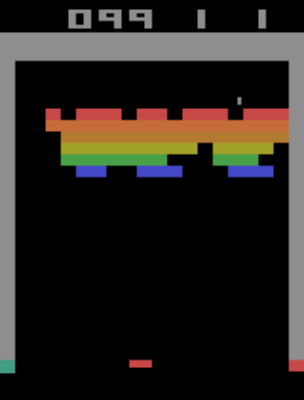
\includegraphics[width=\imgscale\textwidth]{figures/experiments/environments/breakout.png}
        \caption{\BreakoutName}
        \label{fig:environment_breakout}
    \end{subfigure}
    \hfill
    \begin{subfigure}[b]{0.3\textwidth}
        \centering
        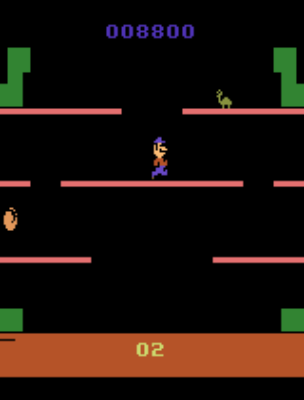
\includegraphics[width=\imgscale\textwidth]{figures/experiments/environments/mario_bros.png}
        \caption{\MarioBrosName}
        \label{fig:environment_mario_bros}
    \end{subfigure}
    \hfill
    \begin{subfigure}[b]{0.3\textwidth}
        \centering
        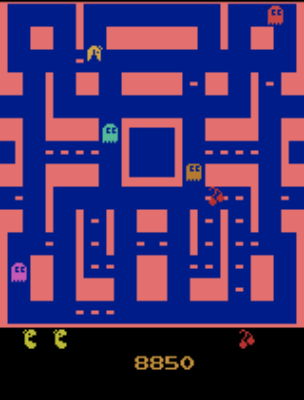
\includegraphics[width=\imgscale\textwidth]{figures/experiments/environments/ms_pacman.png}
        \caption{\MsPacManName}
        \label{fig:environment_ms_pacman}
    \end{subfigure}

    \vspace{0.4cm}

    \begin{subfigure}[b]{0.3\textwidth}
        \centering
        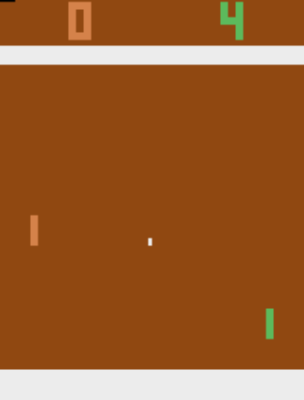
\includegraphics[width=\imgscale\textwidth]{figures/experiments/environments/pong.png}
        \caption{\PongName}
        \label{fig:environment_pong}
    \end{subfigure}
    \hfill
    \begin{subfigure}[b]{0.3\textwidth}
        \centering
        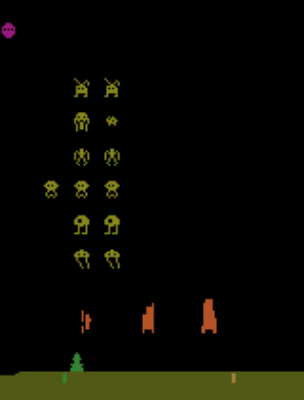
\includegraphics[width=\imgscale\textwidth]{figures/experiments/environments/space_invaders.png}
        \caption{\SpaceInvadersName}
        \label{fig:environment_space_invaders}
    \end{subfigure}
    \hfill
    \begin{subfigure}[b]{0.3\textwidth}
        \centering
        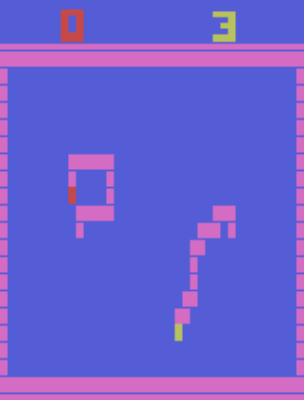
\includegraphics[width=\imgscale\textwidth]{figures/experiments/environments/surround.png}
        \caption{\SurroundName}
        \label{fig:environment_surround}
    \end{subfigure}

    \caption{
        The six Atari environments used to evaluate \glsfmtshort{car}.
    }
    \label{fig:environments}
\end{figure}

The experiments use the six environments described below:
\begingroup
\renewenvironment{samepage}{}{}
\begin{itemize}
    \item \BreakoutName: The agent moves a paddle at the bottom of the screen (Figure~\ref{fig:environment_breakout}) to bounce a ball into a wall of bricks.
    Each broken brick scores one point, and the ball speeds up as the wall is cleared.
    \allowbreak

    \item \MarioBrosName: A platform game (Figure~\ref{fig:environment_mario_bros}) in which the player clears each phase by hitting enemies from below to flip them, then kicking them off the platforms before they recover.
    A central POW block can flip all enemies at once but can only be used a few times per phase.
    \allowbreak

    \item \MsPacManName: The player moves through a maze (Figure~\ref{fig:environment_ms_pacman}), eating pellets while avoiding four ghosts.
    Power pellets temporarily make the ghosts edible.
    \allowbreak

    \item \PongName: A two-player game (Figure~\ref{fig:environment_pong}) in which the agent controls one paddle and must send the ball past the opponent.
    \allowbreak

    \item \SpaceInvadersName: The agent moves a cannon along the bottom of the screen (Figure~\ref{fig:environment_space_invaders}), firing at descending rows of aliens while avoiding their shots and using destructible shields.
    A bonus saucer occasionally crosses the top of the screen.
    \allowbreak

    \item \SurroundName: A two-player game on a grid (Figure~\ref{fig:environment_surround}) in which each player leaves a trail behind a moving cursor.
    The goal is to force the opponent to crash into a trail.
\end{itemize}
\endgroup

\subsection{Neural architecture}

The architecture of the surrogate policies was deliberately kept simple.
The objective of this chapter is not to search for the best-performing architecture, but to obtain surrogate policies that faithfully reproduce the initial policy while remaining easy to analyze.
A standard convolutional architecture was therefore selected because it is sufficient to reach a high \BehaviorReconstructionName on the six environments, as shown in Section~\ref{sec:experiments_policy_performance_and_surrogate_fidelity}.

The surrogate policies use a \gls{cnn} to process the visual observations.
The convolutional part consists of four layers with $16$, $32$, $64$, and $128$ channels, using $4 \times 4$ kernels with a stride of $2$.
Each convolutional layer is followed by a LeakyReLU activation.
The resulting representation is then flattened and passed through a \gls{mlp} that produces the parameters of the action distribution.

The architecture of the \gls{mlp} varies across environments.
For \PongName and \SpaceInvadersName, it contains a single hidden layer with $128$ units.
For the other four environments, it contains three hidden layers with $512$, $256$, and $128$ units.
The size of the output layer matches the number of actions available in each environment: $4$ for \BreakoutName, $18$ for \MarioBrosName, $9$ for \MsPacManName, $6$ for \PongName, $6$ for \SpaceInvadersName, and $5$ for \SurroundName.

Figure~\ref{fig:neural_architecture} illustrates both configurations, together with the shape of the representation produced by each convolutional layer.
Throughout the remainder of this chapter, the analyzed representations are numbered from $1$ to $5$.
These representations correspond to the four convolutional layers and the flattened representation, which are common to all six environments.

The representations produced by the \gls{mlp} are numbered separately.
For \PongName and \SpaceInvadersName, which use a single hidden layer, the representation is numbered $6\text{a}$.
For the other four environments, which use three hidden layers, the representations are numbered $6\text{b}$, $7\text{b}$, and $8\text{b}$.

% ============================================================
% Parameters
% ============================================================

% General text size (in pt), used for the box captions/shapes.
\providecommand{\NeuralArchTextSize}{14}

% Horizontal shift of heads A and B
\providecommand{\NeuralArchBoxShiftX}{0.2cm}

% Margins around boxes A and B (horizontal, and vertical top/bottom set
% independently so the box can be made asymmetric)
\providecommand{\NeuralArchBoxMarginX}{2cm}
\providecommand{\NeuralArchBoxMarginYTop}{1cm}
\providecommand{\NeuralArchBoxMarginYBottom}{0.4cm}

% ------------------------------------------------------------
% Bubbles
% ------------------------------------------------------------
% There are two kinds of bubble (circle + text) in the diagram: the small
% numbered ones (1-5, 6a, 6b/7b/8b) and the two big "A"/"B" ones. For both,
% the same four things can be set independently:
%   - the BUBBLE's position, as an offset from its anchor point
%   - the TEXT's position, as an offset from the SAME anchor point
%   - the TEXT size
%   - the BUBBLE size
% The bubble and the text are two separate nodes, so moving one does not
% move the other. (+X = right, +Y = up.)

% --- Small numbered bubbles -----------------------------------------------
% Anchor = the "-north" point of the box each one marks.
\providecommand{\NeuralArchNumBubbleOffsetX}{0.06cm}
\providecommand{\NeuralArchNumBubbleOffsetY}{0.45cm}
\providecommand{\NeuralArchNumTextOffsetX}{0cm}
\providecommand{\NeuralArchNumTextOffsetY}{0.45cm}
\providecommand{\NeuralArchNumTextSize}{11}       % pt
\providecommand{\NeuralArchNumBubbleSize}{0.7cm}

% --- Big "A"/"B" bubbles ------------------------------------------------
% One common set of parameters for all four of them: the in-diagram A, the
% in-diagram B, and their two counterparts in the legend below. Anchor = the
% top-right corner of box A/B in the diagram, or the local origin of the
% legend's own little picture (see the Legend section).
\providecommand{\NeuralArchLetterBubbleOffsetX}{0cm}
\providecommand{\NeuralArchLetterBubbleOffsetY}{0cm}
\providecommand{\NeuralArchLetterTextOffsetX}{-0.05cm}
\providecommand{\NeuralArchLetterTextOffsetY}{0cm}
\providecommand{\NeuralArchLetterTextSize}{18}    % pt
\providecommand{\NeuralArchLetterBubbleSize}{0.9cm}

% ------------------------------------------------------------
% Layer captions (the "shape + name" text below every layer: Observation,
% Conv1-4, Flatten, and the Dense layers of both heads)
% ------------------------------------------------------------
% Each caption sits a FIXED gap below its OWN box's "-south" anchor (not on
% a shared row), so it stays visually attached to its own layer regardless
% of how tall that layer's box is.
\providecommand{\NeuralArchLayerCaptionOffsetY}{-1.5}
\providecommand{\NeuralArchLayerCaptionTextSize}{14}  % pt, the (non-bold) dimension line
\providecommand{\NeuralArchLayerCaptionSkip}{2pt}     % gap between the dimension and name lines

% ============================================================
% Figure
% ============================================================

\begin{figure}[t]

\centering

\resizebox{\textwidth}{!}{

\begin{tikzpicture}

% --------------------------------------------------------
% General text size
% --------------------------------------------------------

\fontsize{\NeuralArchTextSize pt}
         {\dimexpr\NeuralArchTextSize pt*6/5\relax}
\selectfont

% --------------------------------------------------------
% Bubbles: shared style + fonts + placement macro
% --------------------------------------------------------

% Drawn as a \draw path rather than a \node: a second \node here (alongside
% the text node below) desyncs from its text specifically when this whole
% bubble sits inside a legend node using a non-"center" anchor (TikZ
% typesets that node's content twice -- once to measure, once to render --
% and two sibling \node's positions can drift apart between those passes).
% A path has no such anchor bookkeeping, so it stays put.
\tikzset{
    bubblePath/.style={
        draw,
        thick,
        fill=white
    }
}

\newcommand{\NeuralArchNumFont}{%
    \fontsize{\NeuralArchNumTextSize pt}
             {\dimexpr\NeuralArchNumTextSize pt*6/5\relax}
             \selectfont\bfseries
}
\newcommand{\NeuralArchLetterFont}{%
    \fontsize{\NeuralArchLetterTextSize pt}
             {\dimexpr\NeuralArchLetterTextSize pt*6/5\relax}
             \selectfont\bfseries
}

% This font/size optically centers a bit right of the box TikZ computes
% for a single bold capital, so re-centering it needs a small symmetric
% kern (shifts the ink without changing the measured width).
\newcommand{\NeuralArchCircleLetter}[1]{\kern-0.75pt#1\kern0.75pt}

% A bubble: independent bubble + text nodes, both placed relative to the
% same anchor coordinate, so either can be moved without moving the other.
% The text node is named (#1) so it can be used as a \tikz baseline anchor,
% e.g. when reusing the same bubble inline in the legend.
% #1 = text node name           #2 = anchor coordinate     #3 = bubble offset (X,Y)
% #4 = bubble size              #5 = text offset (X,Y)     #6 = text font   #7 = text content
\newcommand{\NeuralArchBubble}[7]{%
    \draw[bubblePath] ($(#2)+(#3)$) circle ({(#4)/2});
    \node[font=#6, inner sep=0pt, anchor=center] (#1) at ($(#2)+(#5)$) {#7};
}

% Small numbered bubble (1-5, 6a, 6b/7b/8b), anchored on box #3's "-north".
% #1 = optional (X,Y) bubble offset, overriding \NeuralArchNumBubbleOffsetX/Y
% #2 = optional (X,Y) text offset, overriding \NeuralArchNumTextOffsetX/Y
% #3 = box name, #4 = label text
% e.g. \NeuralArchNumLabel[0.2cm,0.5cm][0cm,0.3cm]{c1}{1}
\NewDocumentCommand{\NeuralArchNumLabel}{
    O{\NeuralArchNumBubbleOffsetX,\NeuralArchNumBubbleOffsetY}
    O{\NeuralArchNumTextOffsetX,\NeuralArchNumTextOffsetY}
    m m}{%
    \NeuralArchBubble{numtext-#3}{#3-north}{#1}{\NeuralArchNumBubbleSize}{#2}{\NeuralArchNumFont}{#4}%
}

% Big "A"/"B" bubble -- used identically for the in-diagram A/B and for
% their legend counterparts, so all four share the same parameters.
% #1 = optional (X,Y) bubble offset, overriding \NeuralArchLetterBubbleOffsetX/Y
% #2 = optional (X,Y) text offset, overriding \NeuralArchLetterTextOffsetX/Y
% #3 = anchor coordinate (e.g. boxA.north east, or 0,0 in the legend)
% #4 = letter (A or B)
\NewDocumentCommand{\NeuralArchBigLabel}{
    O{\NeuralArchLetterBubbleOffsetX,\NeuralArchLetterBubbleOffsetY}
    O{\NeuralArchLetterTextOffsetX,\NeuralArchLetterTextOffsetY}
    m m}{%
    \NeuralArchBubble{lettertext-#4}{#3}{#1}{\NeuralArchLetterBubbleSize}{#2}{\NeuralArchLetterFont}{\NeuralArchCircleLetter{#4}}%
}

% --------------------------------------------------------
% Layer captions: shape + name below Observation/Conv/Flatten, all on one
% shared row (see \NeuralArchLayerCaptionRefBox above).
% --------------------------------------------------------

\newcommand{\NeuralArchLayerCaptionFont}{%
    \fontsize{\NeuralArchLayerCaptionTextSize pt}
             {\dimexpr\NeuralArchLayerCaptionTextSize pt*6/5\relax}
             \selectfont
}

% #1 = box name   #2 = dimension text (not bold)   #3 = layer name (bold)
% Named "layercap-#1" so it can be included in a \node[fit=...] (e.g. the
% dashed boxes around heads A/B), since it extends below its box and would
% otherwise be ignored by a fit computed from the box's own corners alone.
\newcommand{\NeuralArchLayerCaption}[3]{%
    \node[align=center, anchor=north, font=\NeuralArchLayerCaptionFont]
        (layercap-#1) at ($(#1-south)+(0,\NeuralArchLayerCaptionOffsetY)$)
        {#2 \\[\NeuralArchLayerCaptionSkip] \bfseries #3};
}


% --------------------------------------------------------
% Observation
% --------------------------------------------------------

\pic[shift={(0,0,0)}] at (0,0,0)
    {Box={
        name=obs,
        caption=,                     % désactivé : on place le texte nous-même (shape + nom)
        xlabel={{"",""}},
        zlabel=,
        fill=ObservationColor,
        height=42,
        width=6,
        depth=42
    }};

\NeuralArchLayerCaption{obs}{64 $\times$ 64 $\times$ 4}{Observation}


% --------------------------------------------------------
% Convolutional trunk
% --------------------------------------------------------

\pic[shift={(2,0,0)}] at (obs-east)
    {Box={
        name=c1,
        caption=,                     % désactivé : on place le texte nous-même (shape + nom)
        xlabel={{"",""}},
        zlabel=,
        fill=ConvColor,
        height=34,
        width=6,
        depth=34
    }};

\NeuralArchLayerCaption{c1}{31 $\times$ 31 $\times$ 16}{Conv}
\NeuralArchNumLabel{c1}{1}

\draw [connection] (obs-east) -- node {\midarrow} (c1-west);


\pic[shift={(1.5,0,0)}] at (c1-east)
    {Box={
        name=c2,
        caption=,
        xlabel={{"",""}},
        zlabel=,
        fill=ConvColor,
        height=26,
        width=9,
        depth=26
    }};

\NeuralArchLayerCaption{c2}{14 $\times$ 14 $\times$ 32}{Conv}
\NeuralArchNumLabel{c2}{2}

\draw [connection] (c1-east) -- node {\midarrow} (c2-west);


\pic[shift={(1.5,0,0)}] at (c2-east)
    {Box={
        name=c3,
        caption=,
        xlabel={{"",""}},
        zlabel=,
        fill=ConvColor,
        height=18,
        width=12,
        depth=18
    }};

\NeuralArchLayerCaption{c3}{6 $\times$ 6 $\times$ 64}{Conv}
\NeuralArchNumLabel{c3}{3}

\draw [connection] (c2-east) -- node {\midarrow} (c3-west);


\pic[shift={(1.5,0,0)}] at (c3-east)
    {Box={
        name=c4,
        caption=,
        xlabel={{"",""}},
        zlabel=,
        fill=ConvColor,
        height=12,
        width=16,
        depth=12
    }};

\NeuralArchLayerCaption{c4}{2 $\times$ 2 $\times$ 128}{Conv}
\NeuralArchNumLabel{c4}{4}

\draw [connection] (c3-east) -- node {\midarrow} (c4-west);


% --------------------------------------------------------
% Flatten
% --------------------------------------------------------

\pic[shift={(1.3,0,0)}] at (c4-east)
    {Box={
        name=flatten,
        caption=,                     % désactivé : on place le texte nous-même
        fill=FlattenColor,
        opacity=0.85,
        height=3,
        width=2,
        depth=42
    }};

\NeuralArchLayerCaption{flatten}{512}{Flatten}
\NeuralArchNumLabel{flatten}{5}

\draw [connection] (c4-east) -- node {\midarrow} (flatten-west);


% ============================================================
% Head A
% ============================================================

\pic[
    shift={(\NeuralArchBoxShiftX,3.2,0)}
] at (flatten-east)
    {Box={
        name=aFc1,
        caption=,
        fill=FcColor,
        opacity=0.7,
        height=3,
        width=2,
        depth=16
    }};
\NeuralArchLayerCaption{aFc1}{128}{Dense}
\NeuralArchNumLabel{aFc1}{6a}

\draw [connection] (flatten-east) -- node {\midarrow} (aFc1-west);


\pic[shift={(2,0,0)}] at (aFc1-east)
    {Box={
        name=aOut,
        caption=,
        fill=OutputColor,
        opacity=0.8,
        height=3,
        width=3,
        depth=8
    }};


\node[align=center]
    at ($(aOut-south)+(0,-1.2)$)
    {\bfseries Distribution};


\draw [connection]
    (aFc1-east) -- node {\midarrow} (aOut-west);


% ------------------------------------------------------------
% Box A
% ------------------------------------------------------------

\node[
    fit=(aFc1-nearnorthwest)
        (aFc1-farsouthwest)
        (aOut-nearsoutheast)
        (aOut-farnortheast)
        (layercap-aFc1),
    inner sep=0pt
] (boxA-fit) {};

\coordinate (boxA-sw) at
    ($(boxA-fit.south west) - (\NeuralArchBoxMarginX,\NeuralArchBoxMarginYBottom)$);
\coordinate (boxA-ne) at
    ($(boxA-fit.north east) + (\NeuralArchBoxMarginX,\NeuralArchBoxMarginYTop)$);

\node[fit=(boxA-sw)(boxA-ne), inner sep=0pt] (boxA) {};

\draw[dashed, rounded corners=0.1cm] (boxA.south west) rectangle (boxA.north east);


% ------------------------------------------------------------
% Label A + bubble
% ------------------------------------------------------------
% Anchor = coin HAUT-DROIT (north east) de la boîte A. Les paramètres
% partagés des bulles A/B (voir section Paramètres/Bulles) déplacent la
% bulle et le texte indépendamment par rapport à ce coin.

\NeuralArchBigLabel{boxA.north east}{A}


% ============================================================
% Head B
% ============================================================

\pic[
    shift={(\NeuralArchBoxShiftX,-3.2,0)}
] at (flatten-east)
    {Box={
        name=bFc1,
        caption=,
        fill=FcColor,
        opacity=0.7,
        height=3,
        width=2,
        depth=30
    }};
\NeuralArchLayerCaption{bFc1}{512}{Dense}
\NeuralArchNumLabel{bFc1}{6b}

\draw [connection] (flatten-east) -- node {\midarrow} (bFc1-west);


\pic[shift={(1.5,0,0)}] at (bFc1-east)
    {Box={
        name=bFc2,
        caption=,
        fill=FcColor,
        opacity=0.7,
        height=3,
        width=2,
        depth=22
    }};
\NeuralArchLayerCaption{bFc2}{256}{Dense}
\NeuralArchNumLabel{bFc2}{7b}

\draw [connection]
    (bFc1-east) -- node {\midarrow} (bFc2-west);


\pic[shift={(1.5,0,0)}] at (bFc2-east)
    {Box={
        name=bFc3,
        caption=,
        fill=FcColor,
        opacity=0.7,
        height=3,
        width=2,
        depth=16
    }};
\NeuralArchLayerCaption{bFc3}{128}{Dense}
\NeuralArchNumLabel{bFc3}{8b}

\draw [connection]
    (bFc2-east) -- node {\midarrow} (bFc3-west);


\pic[shift={(1.5,0,0)}] at (bFc3-east)
    {Box={
        name=bOut,
        caption=,
        fill=OutputColor,
        opacity=0.8,
        height=3,
        width=3,
        depth=8
    }};


\node[align=center]
    at ($(bOut-south)+(0,-1.2)$)
    {\bfseries Distribution};


\draw [connection]
    (bFc3-east) -- node {\midarrow} (bOut-west);


% ------------------------------------------------------------
% Box B
% ------------------------------------------------------------

\node[
    fit=(bFc1-nearnorthwest)
        (bFc1-farsouthwest)
        (bOut-nearsoutheast)
        (bOut-farnortheast)
        (layercap-bFc1)
        (layercap-bFc2)
        (layercap-bFc3),
    inner sep=0pt
] (boxB-fit) {};

\coordinate (boxB-sw) at
    ($(boxB-fit.south west) - (\NeuralArchBoxMarginX,\NeuralArchBoxMarginYBottom)$);
\coordinate (boxB-ne) at
    ($(boxB-fit.north east) + (\NeuralArchBoxMarginX,\NeuralArchBoxMarginYTop)$);

\node[fit=(boxB-sw)(boxB-ne), inner sep=0pt] (boxB) {};

\draw[dashed, rounded corners=0.1cm] (boxB.south west) rectangle (boxB.north east);


% ------------------------------------------------------------
% Label B + bubble
% ------------------------------------------------------------
% Idem pour le label B : ancre = coin HAUT-DROIT de la boîte B, mêmes
% paramètres partagés que le label A.

\NeuralArchBigLabel{boxB.north east}{B}


% ============================================================
% Legend
% ============================================================

\node[
    align=center,
    anchor=north,
    yshift=-0.3cm
] at (current bounding box.south) {

    % Circle A -- same \NeuralArchBigLabel macro and parameters as the
    % in-diagram A, anchored on the local origin of this mini picture.
    \tikz[baseline=(lettertext-A.base)]{
        \NeuralArchBigLabel{0,0}{A}
    }
    \quad Pong, Space Invaders
    \qquad\qquad

    % Circle B -- idem, same macro and parameters as the in-diagram B.
    \tikz[baseline=(lettertext-B.base)]{
        \NeuralArchBigLabel{0,0}{B}
    }
    \quad Breakout, Mario Bros, Ms.\ Pac-Man, Surround

};


\end{tikzpicture}

}

\caption{
    Architecture of the surrogate policies.
}

\label{fig:neural_architecture}

\end{figure}


\subsection{Other \gls{car} parameters}

Several other parameters must be defined for the different stages of the \gls{car} pipeline.
These parameters are less critical to the overall methodology than those discussed above, but they still need to be specified to reproduce the experiments.
Since each stage introduces its own configuration choices, there are too many parameters to discuss them all in detail.
The main parameters used across the experiments are summarized in Table~\ref{tab:experiments_parameters}.
All these parameters are provided to the pipeline through the modular configuration file introduced in Section~\ref{sec:experiments_software_implementation}.
Each stage reads its own section of this file, so that a parameter can be changed, or a component replaced, without modifying the code of the pipeline.

\begin{table}[t]
    \centering
    \begin{tabularx}{0.92\linewidth}{@{}lX@{}}
        \toprule
        \multicolumn{2}{@{}l}{\textbf{Environment configuration}} \\
        \midrule
        Frame size                              & $64 \times 64$ \\
        Frames stacked per observation          & $4$ \\
        Frame skip                              & $5$ \\
        Sticky-action probability               & $0.05$ \\
        \addlinespace
        \midrule
        \multicolumn{2}{@{}l}{\textbf{Initial policy training}} \\
        \midrule
        Algorithm                               & \gls{ppo} \\
        Optimizer                               & Adam \\
        Learning rate                           & $1.5 \times 10^{-4}$ \\
        GAE $\lambda$                           & $0.95$ \\
        Policy clipping $\varepsilon$           & $0.1$ \\
        Value-function clipping                 & $10$ \\
        Entropy coefficient                     & $0.01$ \\
        KL coefficient                          & $0.5$ \\
        Epochs per update                       & $10$ \\
        Gradient clipping (global norm)         & $100$ \\
        \addlinespace
        \midrule
        \multicolumn{2}{@{}l}{\textbf{Surrogate policy training}} \\
        \midrule
        Surrogate policies per environment      & $3$ \\
        Observation--action pairs per dataset   & $\geq 10^{6}$ \\
        Batch size                              & $2048$ \\
        Optimizer                               & Adam \\
        Learning rate                           & $1 \times 10^{-4}$ \\
        \addlinespace
        \midrule
        \multicolumn{2}{@{}l}{\textbf{Latent space analysis}} \\
        \midrule
        Embedding per surrogate policy       & $20\,000$ \\
        Clustering algorithm                    & $k$-means \\
        Distance                                & Euclidean distance \\
        Number of clusters $K$                  & $2$ to $20$ \\
        \bottomrule
    \end{tabularx}
    \caption{Main experimental parameters.}
    \label{tab:experiments_parameters}
\end{table}

These settings are specific to the experiments presented in this chapter and do not restrict the \gls{car} methodology itself.
The different stages of the pipeline are modular and can be configured or replaced depending on the application.
The evaluation metrics provide an objective basis for comparing these alternatives and assessing their effect on the consistency and meaningfulness of the resulting clusters.

\section{Policy Performance and Surrogate Fidelity}
\label{sec:experiments_policy_performance_surrogate_fidelity}

This section reports the results of training the initial and surrogate policies for \gls{car}, applied to the six environments.
The first part verifies that the initial policies reach a competent level of play and evaluates how faithfully the surrogate policies reproduce their behavior using the \BehaviorReconstructionName.

\subsection{Initial policy training}
\label{ssec:initial_policy_training}

% Spacing specific to this figure (tuned for its own subfigure heights --
% do not share these with other multi-subfigure figures, see
% figures/experiments/latent_space_curves_by_metric.tex
% for that figure's own copies).
\newcommand{\PolicyTrainingSubfigCaptionSkip}{-0.4cm} % space between a subfigure's plot and its own caption
\newcommand{\PolicyTrainingSubfigSpacing}{0.4cm}   % vertical space between consecutive subfigures
\newcommand{\PolicyTrainingSubfigLegendSpacing}{0.2cm} % vertical space between the last subfigure and the shared legend
\newcommand{\PolicyTrainingSubfigHeight}{0.4\linewidth} % height of each subfigure's plot (controls this figure's overall scale)

\begin{figure}[t]
    \centering
    \begin{subfigure}[b]{\textwidth}
        \centering
        \captionsetup{skip=\PolicyTrainingSubfigCaptionSkip}
        \input{figures/experiments/initial_policy_training.tex}
        \caption{Training of the initial policies with \glsfmtshort{ppo}.}
        \label{fig:initial_policy_training}
    \end{subfigure}

    \vspace{\PolicyTrainingSubfigSpacing}

    \begin{subfigure}[b]{\textwidth}
        \centering
        \captionsetup{skip=\PolicyTrainingSubfigCaptionSkip}
        \input{figures/experiments/surrogate_policy_training.tex}
        \caption{Training action loss of the surrogate policies.}
        \label{fig:surrogate_policy_training}
    \end{subfigure}

    \vspace{\PolicyTrainingSubfigLegendSpacing}
    {\hypersetup{pdfborder={0 0 0}}\ref{policyTrainingLegend}}
    \caption{Training of the initial and surrogate policies.}
    \label{fig:policy_training}
\end{figure}


Figure~\ref{fig:initial_policy_training} shows how the initial policies improve during \gls{ppo} training.
For each environment, the mean episode return is normalized so that $0\%$ and $100\%$ correspond to the lowest and highest mean return observed during that run.
In every environment the return increases and then reaches a plateau, at which point training is stopped.
The number of iterations required to reach this plateau varies from a few hundred, for \PongName, to several thousand, for \SurroundName and \MsPacManName.
For the subsequent analysis, the checkpoint with the best performance is retained rather than the final checkpoint.

To confirm that the trained policies play competently, their scores are compared with the reference scores reported by \parencite{machado2017revisitingarcadelearningenvironment}.
Each initial policy reaches a score of the same order as these references, so it constitutes a reasonable target for imitation.

\subsection{Surrogate policy training}
\label{ssec:surrogate_policy_training}

Figure~\ref{fig:surrogate_policy_training} shows, for each environment, the training action loss of the three surrogate policies.
In all cases, the loss decreases smoothly, and the three independently trained policies converge to the same value.

We further evaluate the ability of the surrogate policies to replicate the behavior of the initial policies using the \BehaviorReconstructionName (Table~\ref{tab:behavior_reconstruction}).
The surrogate policies reach a \BehaviorReconstructionName of $0.96$ on average over 100 evaluation episodes, ranging from $0.83$ for \BreakoutName to $1.00$ for \MsPacManName and \SurroundName.
They therefore reproduce the decisions of the initial policies closely enough for their \glspl{lr} to be analyzed.

\begin{table}[t]
\centering
\resizebox{0.6\linewidth}{!}{
    \begin{tblr}{
        colspec={|c|c|},
        hlines,
        vlines,
        row{1} = {font=\bfseries, halign=c, valign=m}
    }
        Environment     & \textit{Behavior Reconstruction} \\
        Breakout        & 0.83 $\pm$0.03 \\
        Mario Bros      & 0.99 $\pm$0.03 \\
        Ms.\ Pac-Man    & 1.00 $\pm$0.03 \\
        Pong            & 0.95 $\pm$0.01 \\
        Space Invaders  & 0.97 $\pm$0.07 \\
        Surround        & 1.00 $\pm$0.01 \\
    \end{tblr}
}
\caption{Evaluation of \BehaviorReconstructionName across the six Atari environments.}
\label{tab:behavior_reconstruction}
\end{table}


\section{Clustering Quality of the Latent Space}
\label{sec:experiments_clustering_quality_of_the_latent_space}

This section analyzes the \gls{ls} of the surrogate policies using \gls{cu}, \gls{as}, and \gls{acu}.
To do so, a random subset of $20\,000$ observations is selected for each environment.
This subset is then embedded into the \gls{ls} of each surrogate policy at each analyzed layer.
This produces a point cloud for each combination of environment, surrogate policy, and layer.
Each point cloud is partitioned using $k$-means clustering \parencite{macqueen1967multivariate} for each number of clusters from $2$ to $20$.

The three metrics are then computed from these point clouds and their corresponding clusterings.
Their interpretation, detailed in Section~\ref{sec:clustering_agent_representations_evaluation_metrics}, is briefly recalled here:
\begin{itemize}
    \item \textbf{\gls{cu}} measures the agreement between the partitions obtained from independently trained surrogate policies.
    A value close to $1$ indicates that the surrogate policies group the observations in the same way, while a value close to $0$ indicates an agreement no better than chance.
    Since it relies on the \gls{ari}, a value of $0.5$ already corresponds to a substantial agreement.
    \item \textbf{\gls{as}} measures how far the latent partitions are from three trivial baselines: the clustering of the raw observations, of the action distribution of the initial policy, and of untrained networks.
    A value close to $1$ indicates that the clusters capture an abstraction learned by the policy, while a value close to $0$ indicates that they merely reproduce one of these baselines.
    \item \textbf{\gls{acu}} subtracts the agreement explained by these baselines from \gls{cu}.
    A value close to $1$ indicates that the surrogate policies converge toward a partition that is both reproducible and non-trivial, providing the strongest support for the \RepresentationConvergenceHypothesisName.
    A value close to $0$, or negative, indicates that the observed agreement is largely explained by the baselines.
\end{itemize}
A high \gls{cu} alone is therefore not sufficient, since it can result from a trivial structure shared by all networks.
It is the combination of a high \gls{cu} and a high \gls{as}, summarized by \gls{acu}, that supports the existence of a stable conceptual organization.

The full results across all environments and analyzed layers are reported in Appendix~\ref{chap:additional_results}.
Two complementary analyses are then conducted on these results.
First, the evolution of the three metrics across the different layers is examined to study the effect of representation depth.
Second, for each environment, the layer achieving the highest average \gls{acu} is selected and analyzed in more detail across the different numbers of clusters.

\subsection{Analysis across layers}

The first analysis examines how the three metrics evolve with the depth of the analyzed layer.
For each layer, \gls{cu}, \gls{as}, and \gls{acu} are averaged over the tested cluster numbers.
Figure~\ref{fig:latent_space_curves_by_layer_depth} reports these averages as a function of layer depth.

% Spacing specific to this figure (tuned for its own subfigure heights --
% do not share these with other multi-subfigure figures, see
% figures/experiments/latent_space_curves_by_metric.tex
% and figures/experiments/policy_training.tex for those figures' own copies).
\newcommand{\LatentCurvesByDepthSubfigCaptionSkip}{0.1cm} % space between a subfigure's plot and its own caption
\newcommand{\LatentCurvesByDepthSubfigSpacing}{-0.2cm}   % vertical space between consecutive subfigures
\newcommand{\LatentCurvesByDepthSubfigLegendSpacing}{0.2cm} % vertical space between the last subfigure and the shared legend
\newcommand{\LatentCurvesByDepthSubfigHeight}{0.33\linewidth} % height of each subfigure's plot (controls this figure's overall scale)

\begin{figure}[t]
    \centering
    \begin{subfigure}[b]{\textwidth}
        \centering
        \captionsetup{skip=\LatentCurvesByDepthSubfigCaptionSkip}
        \resizebox{\linewidth}{!}{
        \begin{tikzpicture}
        \begin{axis}[
            xlabel={Layer depth},
            ylabel={\gls{cu}},
            grid=major,
            xmin=1, xmax=8,
            xtick distance=1,
            ymin=0, ymax=1,
            ytick distance=0.25,
            ymajorgrids=true,
            width=\linewidth,
            height=\LatentCurvesByDepthSubfigHeight,
        ]
            \addplot[color=breakoutColor, mark=\breakoutMark, mark size=\breakoutMarkSize] coordinates {
                (1,0.85) (2,0.73) (3,0.57) (4,0.50) (5,0.50) (6,0.59) (7,0.50) (8,0.51)
            };
            \addplot[color=marioBrosColor, mark=\marioBrosMark, mark size=\marioBrosMarkSize] coordinates {
                (1,0.62) (2,0.68) (3,0.62) (4,0.55) (5,0.55) (6,0.48) (7,0.40) (8,0.37)
            };
            \addplot[color=msPacmanColor, mark=\msPacmanMark, mark size=\msPacmanMarkSize] coordinates {
                (1,0.78) (2,0.72) (3,0.68) (4,0.70) (5,0.70) (6,0.58) (7,0.51) (8,0.58)
            };
            \addplot[color=pongColor, mark=\pongMark, mark size=\pongMarkSize] coordinates {
                (1,0.62) (2,0.65) (3,0.48) (4,0.50) (5,0.50) (6,0.31)
            };
            \addplot[color=spaceInvadersColor, mark=\spaceInvadersMark, mark size=\spaceInvadersMarkSize] coordinates {
                (1,0.75) (2,0.81) (3,0.74) (4,0.63) (5,0.63) (6,0.49)
            };
            \addplot[color=surroundColor, mark=\surroundMark, mark size=\surroundMarkSize] coordinates {
                (1,0.70) (2,0.58) (3,0.66) (4,0.65) (5,0.65) (6,0.59) (7,0.49) (8,0.54)
            };
            \addplot[black, dashed, thick, domain=1:8, samples=2, forget plot] {-0.036*x+0.748};
        \end{axis}
        \end{tikzpicture}
        }
        \caption{\glsfmtshort{cu} with respect to the layer depth.}
    \end{subfigure}
    \vspace{\LatentCurvesByDepthSubfigSpacing}

    \begin{subfigure}[b]{\textwidth}
        \centering
        \captionsetup{skip=\LatentCurvesByDepthSubfigCaptionSkip}
        \resizebox{\linewidth}{!}{
        \begin{tikzpicture}
        \begin{axis}[
            xlabel={Layer depth},
            ylabel={\gls{as}},
            grid=major,
            xmin=1, xmax=8,
            xtick distance=1,
            ymin=0, ymax=1,
            ytick distance=0.25,
            ymajorgrids=true,
            width=\linewidth,
            height=\LatentCurvesByDepthSubfigHeight,
        ]
            \addplot[color=breakoutColor, mark=\breakoutMark, mark size=\breakoutMarkSize] coordinates {
                (1,0.15) (2,0.28) (3,0.44) (4,0.76) (5,0.76) (6,0.82) (7,0.79) (8,0.76)
            };
            \addplot[color=marioBrosColor, mark=\marioBrosMark, mark size=\marioBrosMarkSize] coordinates {
                (1,0.44) (2,0.54) (3,0.62) (4,0.66) (5,0.66) (6,0.71) (7,0.83) (8,0.68)
            };
            \addplot[color=msPacmanColor, mark=\msPacmanMark, mark size=\msPacmanMarkSize] coordinates {
                (1,0.19) (2,0.27) (3,0.35) (4,0.41) (5,0.41) (6,0.55) (7,0.64) (8,0.60)
            };
            \addplot[color=pongColor, mark=\pongMark, mark size=\pongMarkSize] coordinates {
                (1,0.33) (2,0.59) (3,0.91) (4,0.95) (5,0.95) (6,0.94)
            };
            \addplot[color=spaceInvadersColor, mark=\spaceInvadersMark, mark size=\spaceInvadersMarkSize] coordinates {
                (1,0.28) (2,0.45) (3,0.54) (4,0.72) (5,0.72) (6,0.74)
            };
            \addplot[color=surroundColor, mark=\surroundMark, mark size=\surroundMarkSize] coordinates {
                (1,0.27) (2,0.45) (3,0.56) (4,0.49) (5,0.49) (6,0.57) (7,0.72) (8,0.71)
            };
            \addplot[black, dashed, thick, domain=1:8, samples=2, forget plot] {0.069*x+0.302};
        \end{axis}
        \end{tikzpicture}
        }
        \caption{\glsfmtshort{as} with respect to the layer depth.}
    \end{subfigure}
    \vspace{\LatentCurvesByDepthSubfigSpacing}

    \begin{subfigure}[b]{\textwidth}
        \centering
        \captionsetup{skip=\LatentCurvesByDepthSubfigCaptionSkip}
        \resizebox{\linewidth}{!}{
        \begin{tikzpicture}
        \begin{axis}[
            xlabel={Layer depth},
            ylabel={\gls{acu}},
            grid=major,
            xmin=1, xmax=8,
            xtick distance=1,
            ymin=-0.2, ymax=1,
            ytick distance=0.2,
            ymajorgrids=true,
            width=\linewidth,
            height=\LatentCurvesByDepthSubfigHeight,
        ]
            \addplot[color=breakoutColor, mark=\breakoutMark, mark size=\breakoutMarkSize] coordinates {
                (1,0.00) (2,0.01) (3,0.01) (4,0.27) (5,0.27) (6,0.41) (7,0.29) (8,0.27)
            };
            \addplot[color=marioBrosColor, mark=\marioBrosMark, mark size=\marioBrosMarkSize] coordinates {
                (1,0.06) (2,0.22) (3,0.24) (4,0.21) (5,0.21) (6,0.19) (7,0.23) (8,0.05)
            };
            \addplot[color=msPacmanColor, mark=\msPacmanMark, mark size=\msPacmanMarkSize] coordinates {
                (1,-0.04) (2,-0.01) (3,0.04) (4,0.10) (5,0.10) (6,0.14) (7,0.15) (8,0.17)
            };
            \addplot[color=pongColor, mark=\pongMark, mark size=\pongMarkSize] coordinates {
                (1,-0.05) (2,0.24) (3,0.39) (4,0.45) (5,0.45) (6,0.26)
            };
            \addplot[color=spaceInvadersColor, mark=\spaceInvadersMark, mark size=\spaceInvadersMarkSize] coordinates {
                (1,0.03) (2,0.25) (3,0.28) (4,0.35) (5,0.35) (6,0.24)
            };
            \addplot[color=surroundColor, mark=\surroundMark, mark size=\surroundMarkSize] coordinates {
                (1,-0.02) (2,0.03) (3,0.22) (4,0.14) (5,0.14) (6,0.16) (7,0.20) (8,0.25)
            };
            \addplot[black, dashed, thick, domain=1:8, samples=2, forget plot] {0.033*x+0.049};
        \end{axis}
        \end{tikzpicture}
        }
        \caption{\glsfmtshort{acu} with respect to the layer depth.}
    \end{subfigure}

    \vspace{\LatentCurvesByDepthSubfigLegendSpacing}
    {\hypersetup{pdfborder={0 0 0}}\ref{policyTrainingLegend}}

    \caption{\glsfmtshort{cu}, \glsfmtshort{as}, and \glsfmtshort{acu} averaged over cluster numbers as a function of layer depth.}
    \label{fig:latent_space_curves_by_layer_depth}
\end{figure}

Across environments, \gls{cu} tends to be highest in the earliest layers and decreases with depth.
\gls{as} follows the opposite trend and generally increases as the representation becomes less tied to the raw observation, the action distribution, and the network's initialization.
This increase is however not monotonic in the deepest layers.
For \MarioBrosName and \MsPacManName, \gls{as} decreases at the last layer, from $0.83$ to $0.68$ and from $0.64$ to $0.60$ respectively, as the latent clustering becomes closer to the clustering of the action distribution, this layer being directly followed by the output layer.
As \gls{acu} combines these two effects, its evolution depends on the environment.

The corresponding linear fits show that \gls{cu} decreases from $0.72$ at the first layer to $0.50$ at the last, with a slope of approximately $-0.04$ per layer, while \gls{as} increases from $0.28$ to $0.69$, with a slope of approximately $+0.06$ per layer.
Over the same range, \gls{acu} increases more moderately from $0.00$ to $0.19$, with a slope of approximately $+0.03$ per layer.
This suggests that, despite the environment-specific variations, deeper representations tend on average to provide a better trade-off between \gls{cu} and \gls{as}.

\subsection{Analysis of the selected layers}

The second analysis examines the effect of the number of clusters on the three metrics.
For each environment, the layer with the highest average \gls{acu} across the tested cluster numbers is selected.
Table~\ref{tab:latent_space_best_layer} reports the selected layer, together with the corresponding average \gls{cu}, \gls{as}, and \gls{acu}.

\begin{table}[t]
\centering
\resizebox{0.8\linewidth}{!}{
    \begin{tblr}{
        colspec={|c|c|c|c|c|},
        hlines,
        vlines,
        row{1} = {font=\bfseries, halign=c, valign=m}
    }
        Environment     & Layer & \gls{cu}        & \gls{as}        & \gls{acu}       \\
        \BreakoutName        & 6b    & 0.59 $\pm$0.06  & 0.82 $\pm$0.05  & 0.41 $\pm$0.06  \\
        \MarioBrosName      & 3     & 0.62 $\pm$0.12  & 0.62 $\pm$0.15  & 0.24 $\pm$0.10  \\
        \MsPacManName    & 8b    & 0.58 $\pm$0.08  & 0.60 $\pm$0.05  & 0.17 $\pm$0.06  \\
        \PongName            & 4     & 0.50 $\pm$0.04  & 0.95 $\pm$0.03  & 0.45 $\pm$0.06  \\
        \SpaceInvadersName  & 4     & 0.63 $\pm$0.11  & 0.73 $\pm$0.06  & 0.35 $\pm$0.09  \\
        \SurroundName        & 8b    & 0.54 $\pm$0.10  & 0.71 $\pm$0.05  & 0.25 $\pm$0.06  \\
    \end{tblr}
}
\caption[Layer maximizing the average \glsfmtshort{acu} in each environment.]{Layer that maximizes the average \glsfmtshort{acu} across $K \in [2,20]$ for each environment, together with the corresponding average \glsfmtshort{cu}, \glsfmtshort{as}, and \glsfmtshort{acu} over $K$.}
\label{tab:latent_space_best_layer}
\end{table}


Figure~\ref{fig:latent_space_curves_by_metric} reports the evolution of \gls{cu}, \gls{as}, and \gls{acu} as the number of clusters varies.
\PongName achieves the highest average \gls{acu} among the six environments, with a value of $0.45 \pm 0.06$.
This results from a moderate \gls{cu} combined with an \gls{as} that saturates from the third layer onward.
In contrast, \MsPacManName achieves the lowest \gls{as}, with $0.60 \pm 0.05$.
The resulting \gls{acu}, $0.17 \pm 0.06$, is the lowest across the six environments.

% Spacing specific to this figure (tuned for its own subfigure heights --
% do not share these with other multi-subfigure figures, see
% figures/experiments/policy_training.tex for that figure's own copies).
\newcommand{\LatentCurvesSubfigCaptionSkip}{0.1cm} % space between a subfigure's plot and its own caption
\newcommand{\LatentCurvesSubfigSpacing}{-0.2cm}   % vertical space between consecutive subfigures
\newcommand{\LatentCurvesSubfigLegendSpacing}{0.2cm} % vertical space between the last subfigure and the shared legend
\newcommand{\LatentCurvesSubfigHeight}{0.33\linewidth} % height of each subfigure's plot (controls this figure's overall scale)

\begin{figure}[H]
    \centering
    \begin{subfigure}[b]{\textwidth}
        \centering
        \captionsetup{skip=\LatentCurvesSubfigCaptionSkip}
        \resizebox{\linewidth}{!}{
        \begin{tikzpicture}
        \begin{axis}[
            xlabel={Number of clusters},
            ylabel={\gls{cu}},
            grid=major,
            xmin=1, xmax=20,
            ymin=0, ymax=1,
            ytick distance=0.25,
            ymajorgrids=true,
            width=\linewidth,
            height=\LatentCurvesSubfigHeight,
        ]
            \addplot[color=breakoutColor, mark=\breakoutMark, mark size=\breakoutMarkSize] coordinates {
                (2,0.66) (3,0.57) (4,0.65) (5,0.79) (6,0.59) (7,0.62) (8,0.56) (9,0.56) (10,0.58) (11,0.64) (12,0.59) (13,0.55) (14,0.55) (15,0.54) (16,0.59) (17,0.60) (18,0.53) (19,0.55) (20,0.55)
            };
            \addplot[color=marioBrosColor, mark=\marioBrosMark, mark size=\marioBrosMarkSize] coordinates {
                (2,0.99) (3,0.84) (4,0.58) (5,0.75) (6,0.54) (7,0.57) (8,0.57) (9,0.66) (10,0.62) (11,0.62) (12,0.58) (13,0.62) (14,0.59) (15,0.55) (16,0.50) (17,0.56) (18,0.59) (19,0.54) (20,0.52)
            };
            \addplot[color=msPacmanColor, mark=\msPacmanMark, mark size=\msPacmanMarkSize] coordinates {
                (2,0.66) (3,0.78) (4,0.58) (5,0.60) (6,0.67) (7,0.64) (8,0.64) (9,0.62) (10,0.59) (11,0.59) (12,0.53) (13,0.62) (14,0.61) (15,0.48) (16,0.48) (17,0.45) (18,0.49) (19,0.48) (20,0.46)
            };
            \addplot[color=pongColor, mark=\pongMark, mark size=\pongMarkSize] coordinates {
                (2,0.60) (3,0.52) (4,0.58) (5,0.49) (6,0.44) (7,0.51) (8,0.58) (9,0.48) (10,0.50) (11,0.52) (12,0.49) (13,0.46) (14,0.50) (15,0.45) (16,0.46) (17,0.47) (18,0.48) (19,0.47) (20,0.53)
            };
            \addplot[color=spaceInvadersColor, mark=\spaceInvadersMark, mark size=\spaceInvadersMarkSize] coordinates {
                (2,0.31) (3,0.73) (4,0.92) (5,0.69) (6,0.61) (7,0.57) (8,0.64) (9,0.61) (10,0.61) (11,0.66) (12,0.58) (13,0.52) (14,0.56) (15,0.63) (16,0.67) (17,0.63) (18,0.63) (19,0.68) (20,0.64)
            };
            \addplot[color=surroundColor, mark=\surroundMark, mark size=\surroundMarkSize] coordinates {
                (2,0.77) (3,0.75) (4,0.67) (5,0.54) (6,0.52) (7,0.55) (8,0.52) (9,0.58) (10,0.61) (11,0.59) (12,0.51) (13,0.52) (14,0.50) (15,0.46) (16,0.50) (17,0.45) (18,0.43) (19,0.43) (20,0.43)
            };
        \end{axis}
        \end{tikzpicture}
        }
        \caption{\glsfmtshort{cu} with respect to the number of clusters.}
    \end{subfigure}
    \vspace{\LatentCurvesSubfigSpacing}

    \begin{subfigure}[b]{\textwidth}
        \centering
        \captionsetup{skip=\LatentCurvesSubfigCaptionSkip}
        \resizebox{\linewidth}{!}{
        \begin{tikzpicture}
        \begin{axis}[
            xlabel={Number of clusters},
            ylabel={\gls{as}},
            grid=major,
            xmin=1, xmax=20,
            ymin=0, ymax=1,
            ytick distance=0.25,
            ymajorgrids=true,
            width=\linewidth,
            height=\LatentCurvesSubfigHeight,
        ]
            \addplot[color=breakoutColor, mark=\breakoutMark, mark size=\breakoutMarkSize] coordinates {
                (2,0.62) (3,0.83) (4,0.74) (5,0.82) (6,0.85) (7,0.85) (8,0.85) (9,0.85) (10,0.83) (11,0.82) (12,0.85) (13,0.85) (14,0.84) (15,0.83) (16,0.83) (17,0.83) (18,0.84) (19,0.85) (20,0.83)
            };
            \addplot[color=marioBrosColor, mark=\marioBrosMark, mark size=\marioBrosMarkSize] coordinates {
                (2,0.00) (3,0.66) (4,0.63) (5,0.65) (6,0.64) (7,0.62) (8,0.63) (9,0.62) (10,0.69) (11,0.69) (12,0.64) (13,0.66) (14,0.62) (15,0.64) (16,0.67) (17,0.65) (18,0.66) (19,0.64) (20,0.69)
            };
            \addplot[color=msPacmanColor, mark=\msPacmanMark, mark size=\msPacmanMarkSize] coordinates {
                (2,0.56) (3,0.59) (4,0.47) (5,0.57) (6,0.56) (7,0.54) (8,0.55) (9,0.56) (10,0.60) (11,0.58) (12,0.62) (13,0.59) (14,0.59) (15,0.65) (16,0.65) (17,0.68) (18,0.66) (19,0.66) (20,0.67)
            };
            \addplot[color=pongColor, mark=\pongMark, mark size=\pongMarkSize] coordinates {
                (2,0.99) (3,0.99) (4,0.98) (5,0.99) (6,0.97) (7,0.96) (8,0.97) (9,0.96) (10,0.93) (11,0.94) (12,0.96) (13,0.93) (14,0.93) (15,0.93) (16,0.93) (17,0.91) (18,0.90) (19,0.90) (20,0.91)
            };
            \addplot[color=spaceInvadersColor, mark=\spaceInvadersMark, mark size=\spaceInvadersMarkSize] coordinates {
                (2,0.94) (3,0.80) (4,0.69) (5,0.71) (6,0.71) (7,0.75) (8,0.74) (9,0.74) (10,0.75) (11,0.69) (12,0.67) (13,0.68) (14,0.71) (15,0.68) (16,0.68) (17,0.70) (18,0.69) (19,0.74) (20,0.69)
            };
            \addplot[color=surroundColor, mark=\surroundMark, mark size=\surroundMarkSize] coordinates {
                (2,0.66) (3,0.53) (4,0.71) (5,0.70) (6,0.71) (7,0.70) (8,0.71) (9,0.69) (10,0.68) (11,0.71) (12,0.74) (13,0.74) (14,0.73) (15,0.74) (16,0.73) (17,0.75) (18,0.76) (19,0.75) (20,0.76)
            };
        \end{axis}
        \end{tikzpicture}
        }
        \caption{\glsfmtshort{as} with respect to the number of clusters.}
    \end{subfigure}
    \vspace{\LatentCurvesSubfigSpacing}

    \begin{subfigure}[b]{\textwidth}
        \centering
        \captionsetup{skip=\LatentCurvesSubfigCaptionSkip}
        \resizebox{\linewidth}{!}{
        \begin{tikzpicture}
        \begin{axis}[
            xlabel={Number of clusters},
            ylabel={\gls{acu}},
            grid=major,
            xmin=1, xmax=20,
            ymin=-0.2, ymax=1,
            ytick distance=0.2,
            ymajorgrids=true,
            width=\linewidth,
            height=\LatentCurvesSubfigHeight,
        ]
            \addplot[color=breakoutColor, mark=\breakoutMark, mark size=\breakoutMarkSize] coordinates {
                (2,0.28) (3,0.40) (4,0.39) (5,0.61) (6,0.43) (7,0.47) (8,0.41) (9,0.41) (10,0.42) (11,0.46) (12,0.45) (13,0.40) (14,0.39) (15,0.37) (16,0.42) (17,0.43) (18,0.36) (19,0.40) (20,0.38)
            };
            \addplot[color=marioBrosColor, mark=\marioBrosMark, mark size=\marioBrosMarkSize] coordinates {
                (2,0.00) (3,0.50) (4,0.21) (5,0.40) (6,0.18) (7,0.20) (8,0.20) (9,0.27) (10,0.31) (11,0.31) (12,0.23) (13,0.28) (14,0.21) (15,0.19) (16,0.16) (17,0.22) (18,0.25) (19,0.18) (20,0.21)
            };
            \addplot[color=msPacmanColor, mark=\msPacmanMark, mark size=\msPacmanMarkSize] coordinates {
                (2,0.22) (3,0.37) (4,0.05) (5,0.16) (6,0.23) (7,0.18) (8,0.19) (9,0.19) (10,0.19) (11,0.17) (12,0.15) (13,0.21) (14,0.20) (15,0.13) (16,0.12) (17,0.13) (18,0.15) (19,0.14) (20,0.13)
            };
            \addplot[color=pongColor, mark=\pongMark, mark size=\pongMarkSize] coordinates {
                (2,0.59) (3,0.51) (4,0.56) (5,0.48) (6,0.41) (7,0.48) (8,0.56) (9,0.44) (10,0.44) (11,0.46) (12,0.45) (13,0.40) (14,0.43) (15,0.38) (16,0.39) (17,0.38) (18,0.38) (19,0.38) (20,0.44)
            };
            \addplot[color=spaceInvadersColor, mark=\spaceInvadersMark, mark size=\spaceInvadersMarkSize] coordinates {
                (2,0.26) (3,0.53) (4,0.61) (5,0.40) (6,0.32) (7,0.32) (8,0.38) (9,0.36) (10,0.35) (11,0.35) (12,0.26) (13,0.20) (14,0.27) (15,0.31) (16,0.36) (17,0.33) (18,0.32) (19,0.43) (20,0.34)
            };
            \addplot[color=surroundColor, mark=\surroundMark, mark size=\surroundMarkSize] coordinates {
                (2,0.42) (3,0.28) (4,0.38) (5,0.24) (6,0.23) (7,0.24) (8,0.23) (9,0.27) (10,0.29) (11,0.30) (12,0.24) (13,0.26) (14,0.23) (15,0.20) (16,0.23) (17,0.20) (18,0.18) (19,0.18) (20,0.19)
            };
        \end{axis}
        \end{tikzpicture}
        }
        \caption{\glsfmtshort{acu} with respect to the number of clusters.}
    \end{subfigure}

    \vspace{\LatentCurvesSubfigLegendSpacing}
    {\hypersetup{pdfborder={0 0 0}}\ref{policyTrainingLegend}}

    \caption[\glsfmtshort{cu}, \glsfmtshort{as}, and \glsfmtshort{acu} with respect to the number of clusters.]{\glsfmtshort{cu}, \glsfmtshort{as}, and \glsfmtshort{acu} with respect to the number of clusters, for each of the six environments, for the layer that maximizes the average \glsfmtshort{acu} in that environment.}
    \label{fig:latent_space_curves_by_metric}
\end{figure}

% (see Table~\ref{tab:latent_space_best_layer} for the specific layer and average values of each environment)

The quantitative analysis provides a measure of the consistency and abstraction of the identified clusters, but does not directly reveal their semantic content.
The following section therefore provides a qualitative analysis of the clusters to examine the concepts they represent.
\section{Semantic Interpretation of the Clusters}
\label{sec:experiments_semantic_interpretation_of_the_clusters}

The metrics reported in Section~\ref{sec:experiments_clustering_quality_of_the_latent_space} evaluate the \gls{ls} clusterings quantitatively but do not indicate what the resulting clusters actually represent.
This section complements them with a qualitative, hand-labeled inspection of the clusters obtained for each environment.

For each environment, two clusterings are selected for the qualitative analysis.
They are obtained using two different numbers of clusters and may correspond to different layers of the network.
The choice of the layer and the number of clusters is based on the following criteria:
\begin{itemize}
\item \textbf{High \gls{acu}:} The selected clustering should achieve a sufficiently high \gls{acu}, indicating a good balance between consistency and abstraction.
\item \textbf{Manual analysis:} The number of clusters must remain small enough to allow the resulting clusters to be examined manually.
\item \textbf{Limited use of two-cluster partitions:} Clusterings with two clusters often achieve a high \gls{acu}, but provide limited information about the organization of the \gls{ls}. Therefore, at most one of the two selected clusterings uses two clusters, while the other uses a larger number of clusters to provide a more detailed view of the \gls{ls}.
\end{itemize}

Only these two clusterings are discussed below, but the clusters obtained for every analyzed layer can also be inspected.\footnote{Images of the clusters obtained for every analyzed layer have been archived on Zenodo \LinkClusterImages.}

\newcommand{\qualitativeClusterImageScale}{0.20}

\newlength{\qualitativeClusterImageWidth}
\settowidth{\qualitativeClusterImageWidth}{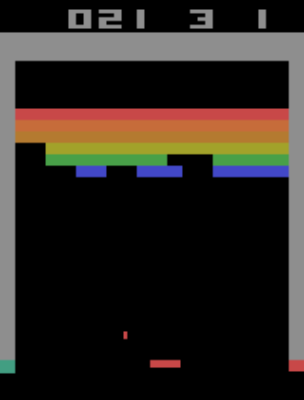
\includegraphics[scale=\qualitativeClusterImageScale]{figures/experiments/pictures/breakout/qualitative/cluster_0/image_1.png}}

% Spacing between the two screenshots of a same cluster.
\newlength{\qualitativeClusterImageGap}
\setlength{\qualitativeClusterImageGap}{0.1cm}

% Spacing between two clusters on the same row of a figure.
\newlength{\qualitativeClusterGap}
\setlength{\qualitativeClusterGap}{0.4cm}

% Vertical spacing between two rows of clusters in a same figure.
\newlength{\qualitativeClusterRowGap}
\setlength{\qualitativeClusterRowGap}{0.3cm}

% The gap is inserted before every cluster except the first one of a figure, so that
% no row carries a trailing gap and every row is centered on the same axis.
\newif\ifqualitativeFirstCluster

% Start of every cluster figure: centers the clusters and applies the row spacing.
\newcommand{\qualitativeClusterFigureSetup}{%
    \centering
    \setlength{\lineskiplimit}{1000pt}%
    \setlength{\lineskip}{\qualitativeClusterRowGap}%
    \qualitativeFirstClustertrue
}

% A cluster shown with two example screenshots, always kept on the same line, labeled with a letter.
\newcommand{\qualitativeClusterTwo}[3]{%
    \ifqualitativeFirstCluster\qualitativeFirstClusterfalse\else\hspace{\qualitativeClusterGap}\fi
    \begin{minipage}[t]{\dimexpr 2\qualitativeClusterImageWidth+\qualitativeClusterImageGap\relax}
        \centering
        \includegraphics[scale=\qualitativeClusterImageScale]{#1}\hspace{\qualitativeClusterImageGap}\includegraphics[scale=\qualitativeClusterImageScale]{#2}\par
        \small\textbf{#3}
    \end{minipage}%
}

\EnableCompactFloats
\newpage
\subsection{\BreakoutName}

Two clusterings are examined for \BreakoutName (Table~\ref{tab:qualitative_breakout_metrics}), obtained at layer 4 with $K=2$ and at layer 6b with $K=5$.

At layer 4 (Figure~\ref{fig:qualitative_breakout_alt}), the partition captures the position of the ball relative to the brick wall.
The ball remains below the wall in cluster A.
The ball has passed behind the wall in cluster B, allowing it to continue clearing bricks without further interaction with the paddle.

At layer 6b (Figure~\ref{fig:qualitative_breakout}), the partition again isolates situations in which the ball has passed behind the wall in cluster E.
It also identifies the digging of a tunnel through the left side of the wall in cluster C.
Finally, it distinguishes different paddle positions at the beginning of the episode in clusters D, F, and G.

The clustering at layer 4 with $K=2$ is almost perfectly reproducible across surrogate policies, with a \gls{cu} of $0.99$ and an \gls{acu} of $0.87$.
The clustering at layer 6b with $K=5$ is less consistent, with a \gls{cu} of $0.79$ and an \gls{acu} of $0.61$, but reveals additional information about the organization of the \gls{ls}.

\vfill
\begin{table}[H]
    \centering
    \begin{tblr}{
        width=\linewidth,
        colspec={Q[c,wd=1.6cm] X[l]},
        cells = {valign=m},
        rowsep=2pt,
        hline{1,Z} = {1pt},
        hline{4} = {0.5pt},
        hline{2,5} = {0.3pt},
        row{1,4} = {bg=black!8, font=\bfseries},
        column{1} = {font=\bfseries}
    }
        \SetCell[c=2]{l} \makebox[1.9cm][l]{Layer 4}\makebox[1.4cm][l]{$K=2$}\makebox[2.75cm][l]{\gls{cu} 0.99}\makebox[2.75cm][l]{\gls{as} 0.88}\gls{acu} 0.87 & \\
        A & The ball is below the brick wall. \\
        B & The ball passes behind the brick wall. \\
        \SetCell[c=2]{l} \makebox[1.9cm][l]{Layer 6b}\makebox[1.4cm][l]{$K=5$}\makebox[2.75cm][l]{\gls{cu} 0.79}\makebox[2.75cm][l]{\gls{as} 0.82}\gls{acu} 0.61 & \\
        C & Digging a tunnel through the left side of the wall. \\
        D & Start of the episode, paddle on the right. \\
        E & The ball is behind the brick wall. \\
        F & Start of the episode, paddle in the middle. \\
        G & Start of the episode, paddle on the left. \\
    \end{tblr}
    \caption{\glsfmtshort{cu}, \glsfmtshort{as}, and \glsfmtshort{acu} of the two clusterings analyzed in the \BreakoutName environment.}
    \label{tab:qualitative_breakout_metrics}
\end{table}
\vfill

\newpage
\vspace*{\fill}
\input{figures/experiments/qualitative_breakout_alt.tex}

\input{figures/experiments/qualitative_breakout.tex}
\vfill

\cleartoleftpage
\subsection{\MarioBrosName}

Two clusterings are examined for \MarioBrosName (Table~\ref{tab:qualitative_mario_bros_metrics}), both obtained at layer 3, with $K=3$ and $K=5$.

With $K=3$ (Figure~\ref{fig:qualitative_mario_bros}), the partition is organized around the location of the action.
Mario fights enemies on the left side of the screen in cluster A.
He fights enemies on the right side of the screen in cluster C.
The POW block is present in cluster B, isolating a fixed and recognizable element of the level.

With $K=5$ (Figure~\ref{fig:qualitative_mario_bros_alt}), the partition provides a more detailed description of the situations occurring in the level.
Mario is on the top-left platform in cluster D.
Mario attacks enemies at the top left in cluster F.
Mario hits enemies from below in cluster H.
Mario simply moves through the level in cluster G.
The POW block remains isolated in cluster E.

Increasing $K$ from $3$ to $5$ lowers \gls{cu} from $0.84$ to $0.75$.
The \gls{as} remains nearly unchanged, with values of $0.66$ and $0.65$.
This results in a decrease in \gls{acu} from $0.50$ to $0.40$.

\vfill
\begin{table}[H]
    \centering
    \begin{tblr}{
        width=\linewidth,
        colspec={Q[c,wd=1.6cm] X[l]},
        cells = {valign=m},
        rowsep=2pt,
        hline{1,Z} = {1pt},
        hline{5} = {0.5pt},
        hline{2,6} = {0.3pt},
        row{1,5} = {bg=black!8, font=\bfseries},
        column{1} = {font=\bfseries}
    }
        \SetCell[c=2]{l} \makebox[1.9cm][l]{Layer 3}\makebox[1.4cm][l]{$K=3$}\makebox[2.75cm][l]{\gls{cu} 0.84}\makebox[2.75cm][l]{\gls{as} 0.66}\gls{acu} 0.50 & \\
        A & Mario fights enemies on the left side of the screen. \\
        B & The POW block is present. \\
        C & Mario fights enemies on the right side of the screen. \\
        \SetCell[c=2]{l} \makebox[1.9cm][l]{Layer 3}\makebox[1.4cm][l]{$K=5$}\makebox[2.75cm][l]{\gls{cu} 0.75}\makebox[2.75cm][l]{\gls{as} 0.65}\gls{acu} 0.40 & \\
        D & Mario is on the top-left platform. \\
        E & The POW block is present. \\
        F & Mario attacks the enemies at the top right. \\
        G & Mario moves through the level. \\
        H & Mario hits enemies from below on the left side. \\
    \end{tblr}
    \caption{\glsfmtshort{cu}, \glsfmtshort{as}, and \glsfmtshort{acu} of the two clusterings analyzed in the \MarioBrosName environment.}
    \label{tab:qualitative_mario_bros_metrics}
\end{table}
\vfill

\newpage
\vspace*{\fill}
\input{figures/experiments/qualitative_mario_bros.tex}

\input{figures/experiments/qualitative_mario_bros_alt.tex}
\vfill

\cleartoleftpage
\subsection{\MsPacManName}

Two clusterings are examined for \MsPacManName (Table~\ref{tab:qualitative_ms_pacman_metrics}), obtained at layer 6b with $K=3$ and at layer 4 with $K=5$.

With $K=3$ (Figure~\ref{fig:qualitative_ms_pacman}), the partition captures the progress and state of the game rather than a specific spatial feature of the observation.
The start of the episode is captured in cluster B.
The middle of the episode is captured in cluster A.
The end of the episode is captured in cluster C.

With $K=5$ (Figure~\ref{fig:qualitative_ms_pacman_alt}), the partition provides a more detailed description of the episode.
The initial animation, during which the character cannot move, is isolated in cluster H.
The beginning of actual play is captured in cluster F.
A situation specific to the game mechanics, in which Pac-Man is in booster mode and waits in front of the ghost spawn to eat the ghosts, is isolated in cluster D.
The end of the episode, when at most one power pellet remains, is separated into two similar clusters, E and G.

The two clusterings have the same \gls{cu} of $0.88$.
The clustering at layer 4 has a lower \gls{as} of $0.47$ compared with $0.52$ at layer 6b.
This results in a lower \gls{acu} of $0.35$ compared with $0.40$.

\vfill
\begin{table}[H]
    \centering
    \begin{tblr}{
        width=\linewidth,
        colspec={Q[c,wd=1.6cm] X[l]},
        cells = {valign=m},
        rowsep=2pt,
        hline{1,Z} = {1pt},
        hline{5} = {0.5pt},
        hline{2,6} = {0.3pt},
        row{1,5} = {bg=black!8, font=\bfseries},
        column{1} = {font=\bfseries}
    }
        \SetCell[c=2]{l} \makebox[1.9cm][l]{Layer 6b}\makebox[1.4cm][l]{$K=3$}\makebox[2.75cm][l]{\gls{cu} 0.88}\makebox[2.75cm][l]{\gls{as} 0.52}\gls{acu} 0.40 & \\
        A & Middle of the episode. \\
        B & Start of the episode. \\
        C & End of the episode. \\
        \SetCell[c=2]{l} \makebox[1.9cm][l]{Layer 4}\makebox[1.4cm][l]{$K=5$}\makebox[2.75cm][l]{\gls{cu} 0.88}\makebox[2.75cm][l]{\gls{as} 0.47}\gls{acu} 0.35 & \\
        D & Pac-Man is in booster mode and waits in front of the ghost spawn to eat the ghosts. \\
        E & End of the episode, at most one power pellet remains (similar to cluster G). \\
        F & Start of the episode. \\
        G & End of the episode, at most one power pellet remains (similar to cluster E). \\
        H & Start-of-episode animation, the character cannot move. \\
    \end{tblr}
    \caption{\glsfmtshort{cu}, \glsfmtshort{as}, and \glsfmtshort{acu} of the two clusterings analyzed in the \MsPacManName environment.}
    \label{tab:qualitative_ms_pacman_metrics}
\end{table}
\vfill

\newpage
\vspace*{\fill}
\input{figures/experiments/qualitative_ms_pacman.tex}

\input{figures/experiments/qualitative_ms_pacman_alt.tex}
\vfill

\newpage
\subsection{\PongName}

Two clusterings are examined for \PongName (Table~\ref{tab:qualitative_pong_metrics}), obtained at layer 2 with $K=2$ and at layer 3 with $K=3$.

At layer 2 (Figure~\ref{fig:qualitative_pong_alt}), the partition separates the observations according to the number of digits in the player's score.
A one-digit score corresponds to cluster A.
A two-digit score corresponds to cluster B.
This reflects the progress of the game, but only through its visual display at the top of the screen.
The partition therefore captures a feature of the observation that provides no information about how the agent plays.

At layer 3 (Figure~\ref{fig:qualitative_pong}), the partition instead follows the vertical position of the ball.
The ball is at the top of the field in cluster C.
It is in the middle of the field in cluster D.
It is at the bottom of the field in cluster E.
This feature directly determines where the agent needs to place its paddle.

The clustering at layer 2 is perfectly reproducible and perfectly abstract, with \gls{cu}, \gls{as}, and \gls{acu} all equal to $1.00$.
The clustering at layer 3 is less consistent, with a \gls{cu} of $0.67$, and reaches a lower \gls{acu} of $0.65$.

\vfill
\begin{table}[H]
    \centering
    \begin{tblr}{
        width=\linewidth,
        colspec={Q[c,wd=1.6cm] X[l]},
        cells = {valign=m},
        rowsep=2pt,
        hline{1,Z} = {1pt},
        hline{4} = {0.5pt},
        hline{2,5} = {0.3pt},
        row{1,4} = {bg=black!8, font=\bfseries},
        column{1} = {font=\bfseries}
    }
        \SetCell[c=2]{l} \makebox[1.9cm][l]{Layer 2}\makebox[1.4cm][l]{$K=2$}\makebox[2.75cm][l]{\gls{cu} 1.00}\makebox[2.75cm][l]{\gls{as} 1.00}\gls{acu} 1.00 & \\
        A & The player's score has two digits. \\
        B & The player's score has one digit. \\
        \SetCell[c=2]{l} \makebox[1.9cm][l]{Layer 3}\makebox[1.4cm][l]{$K=3$}\makebox[2.75cm][l]{\gls{cu} 0.67}\makebox[2.75cm][l]{\gls{as} 0.98}\gls{acu} 0.65 & \\
        C & The ball is at the top. \\
        D & The ball is in the middle. \\
        E & The ball is at the bottom. \\
    \end{tblr}
    \caption{\glsfmtshort{cu}, \glsfmtshort{as}, and \glsfmtshort{acu} of the two clusterings analyzed in the \PongName environment.}
    \label{tab:qualitative_pong_metrics}
\end{table}
\vfill

\newpage
\vspace*{\fill}
\input{figures/experiments/qualitative_pong_alt.tex}

\input{figures/experiments/qualitative_pong.tex}
\vfill

\cleartoleftpage
\subsection{\SpaceInvadersName}

Two clusterings are examined for \SpaceInvadersName (Table~\ref{tab:qualitative_space_invaders_metrics}), obtained at layer 4 with $K=4$ and at layer 2 with $K=5$.

At layer 4 (Figure~\ref{fig:qualitative_space_invaders}), the partition tracks the progression of the episode.
The start of the episode is captured in cluster D.
The middle of the episode is captured in cluster B.
The end of the episode is captured in cluster C.
A specific behavior in which the agent has cleared the leftmost column and is positioned to catch the flying saucer that occasionally crosses the top of the screen is captured in cluster A.

At layer 2 (Figure~\ref{fig:qualitative_space_invaders_alt}), the partition again tracks the progression of the episode.
The start of the episode is captured in cluster G.
The middle of the episode is captured in cluster F.
The end of the episode is captured in cluster I.
Attacking the first two columns of the formation is captured in cluster E.
Trying to catch the flying saucer is captured in cluster H.

The clustering at layer 4 has a \gls{cu} of $0.92$ and a \gls{as} of $0.69$, resulting in a \gls{acu} of $0.61$.
The clustering at layer 2 has the same \gls{cu} of $0.92$, but a lower \gls{as} of $0.49$, resulting in a lower \gls{acu} of $0.41$.

\vfill
\begin{table}[H]
    \centering
    \begin{tblr}{
        width=\linewidth,
        colspec={Q[c,wd=1.6cm] X[l]},
        cells = {valign=m},
        rowsep=2pt,
        hline{1,Z} = {1pt},
        hline{6} = {0.5pt},
        hline{2,7} = {0.3pt},
        row{1,6} = {bg=black!8, font=\bfseries},
        column{1} = {font=\bfseries}
    }
        \SetCell[c=2]{l} \makebox[1.9cm][l]{Layer 4}\makebox[1.4cm][l]{$K=4$}\makebox[2.75cm][l]{\gls{cu} 0.92}\makebox[2.75cm][l]{\gls{as} 0.69}\gls{acu} 0.61 & \\
        A & The left column has been cleared; the flying saucer occasionally appears. \\
        B & Middle of the episode. \\
        C & End of the episode. \\
        D & Start of the episode. \\
        \SetCell[c=2]{l} \makebox[1.9cm][l]{Layer 2}\makebox[1.4cm][l]{$K=5$}\makebox[2.75cm][l]{\gls{cu} 0.92}\makebox[2.75cm][l]{\gls{as} 0.49}\gls{acu} 0.41 & \\
        E & Attacks the first two columns of the formation. \\
        F & Middle of the episode. \\
        G & Start of the episode. \\
        H & Tries to catch the flying saucer. \\
        I & End of the episode. \\
    \end{tblr}
    \caption{\glsfmtshort{cu}, \glsfmtshort{as}, and \glsfmtshort{acu} of the two clusterings analyzed in the \SpaceInvadersName environment.}
    \label{tab:qualitative_space_invaders_metrics}
\end{table}
\vfill

\newpage
\vspace*{\fill}
\input{figures/experiments/qualitative_space_invaders.tex}

\input{figures/experiments/qualitative_space_invaders_alt.tex}
\vfill

\cleartoleftpage
\subsection{\SurroundName}

Two clusterings are examined for \SurroundName (Table~\ref{tab:qualitative_surround_metrics}), obtained at layer 8b with $K=4$ and at layer 7b with $K=6$.

At layer 8b (Figure~\ref{fig:qualitative_surround}), the partition captures the start of the episode in cluster B.
The outcome of the episode, when the opponent loses, is captured in cluster D.
The player's trail is confined to the bottom-left area in cluster A.
The player reaches the top of the level from the left and then moves along the top in cluster C.

At layer 7b (Figure~\ref{fig:qualitative_surround_alt}), the partition again captures the start of the episode in cluster J.
The outcome of the episode, when the opponent loses, is captured in cluster F.
The player moves in the upper-left corner in cluster E.
The player moves in the lower-left corner in cluster G.
The end of the game is played in the lower-left corner in cluster H.
The player crosses the level from the top left to the bottom right in cluster I.

The clustering at layer 8b has a \gls{cu} of $0.67$, a \gls{as} of $0.71$, and a \gls{acu} of $0.38$.
The clustering at layer 7b reaches the same values, with a \gls{cu} of $0.67$, a \gls{as} of $0.71$, and a \gls{acu} of $0.38$.

\vfill
\begin{table}[H]
    \centering
    \begin{tblr}{
        width=\linewidth,
        colspec={Q[c,wd=1.6cm] X[l]},
        cells = {valign=m},
        rowsep=2pt,
        hline{1,Z} = {1pt},
        hline{6} = {0.5pt},
        hline{2,7} = {0.3pt},
        row{1,6} = {bg=black!8, font=\bfseries},
        column{1} = {font=\bfseries}
    }
        \SetCell[c=2]{l} \makebox[1.9cm][l]{Layer 8b}\makebox[1.4cm][l]{$K=4$}\makebox[2.75cm][l]{\gls{cu} 0.67}\makebox[2.75cm][l]{\gls{as} 0.71}\gls{acu} 0.38 & \\
        A & The agent's trail remains confined to the bottom-left area. \\
        B & Start of the episode. \\
        C & The agent moves along the top of the level, arriving from the left. \\
        D & The opponent loses by running into a trail. \\
        \SetCell[c=2]{l} \makebox[1.9cm][l]{Layer 7b}\makebox[1.4cm][l]{$K=6$}\makebox[2.75cm][l]{\gls{cu} 0.67}\makebox[2.75cm][l]{\gls{as} 0.71}\gls{acu} 0.38 & \\
        E & The player moves in the upper-left corner. \\
        F & The opponent loses the confrontation. \\
        G & The player moves in the lower-left corner. \\
        H & The end of the game is played in the lower-left corner. \\
        I & The player starts at the top left and ends at the bottom right. \\
        J & Start of the episode. \\
    \end{tblr}
    \caption{\glsfmtshort{cu}, \glsfmtshort{as}, and \glsfmtshort{acu} of the two clusterings analyzed in the \SurroundName environment.}
    \label{tab:qualitative_surround_metrics}
\end{table}
\vfill

\newpage
\vspace*{\fill}
\input{figures/experiments/qualitative_surround.tex}

\input{figures/experiments/qualitative_surround_alt.tex}
\vfill


\section{Conclusion}
\label{sec:experiments_conclusion}

The quantitative results show that \gls{car} consistently recovers similar clustering structures across independently trained surrogate policies.
Across the six environments, the \gls{cu} frequently exceeds $0.5$, indicating that independently trained policies can develop similarly structured \glspl{lr} \parencite{amezquita2020orchestrating}.
The \gls{cu} also tends to decrease as the network gets deeper, with the highest values generally observed in the earliest layers.
Considering consistency alone would therefore favor the earliest layers of the network.

To complement this analysis, the level of abstraction of these representations must also be considered.
For this purpose, \gls{as} is analyzed and shows that the earliest layers tend to exhibit lower levels of abstraction.
Their representations remain strongly related to the observations and the initial structure of the network.
In the deepest layers, the abstraction can decrease again in some environments, as the latent clustering becomes closer to the clustering of the action distribution.

This highlights the importance of considering both consistency and abstraction when identifying meaningful \glspl{lr}.
The \gls{acu} addresses this limitation by combining these two properties into a single measure, providing a practical criterion for identifying layers that achieve a suitable balance between representational consistency and abstraction.

These quantitative analyses are complemented by the qualitative analysis, which shows that the clusters identified by \gls{car} correspond to interpretable properties of the environment and the agent's behavior.
Across the different environments, the clusters capture recurring aspects such as episode progression, specific game situations, and behavioral patterns.
These observations provide qualitative evidence that the structures recovered by \gls{car} can reflect semantically aspects of the underlying task.

The qualitative analysis also reveals a trade-off associated with the number of clusters.
Increasing the number of clusters allows more specific situations to be distinguished, but tends to reduce the stability of the resulting partitions across surrogate policies.
Finer clusters have less clear semantic boundaries, reducing agreement across independently trained policies.
The choice of the number of clusters therefore involves a trade-off between recovering stable, shared concepts and capturing finer distinctions between situations.

Overall, these results provide empirical support for the assumptions underlying \gls{car}.
Independently trained surrogate policies exhibit a degree of convergence in the organization of their \glspl{lr} that cannot be explained solely by the considered baselines.
The qualitative analysis also shows that these clusters can correspond to meaningful properties of the environment and the agent's behavior.
Taken together, these findings provide empirical support for the \RepresentationConvergenceHypothesisName.



\DisableCompactFloats

\chapter{Conclusion}
\label{chap:conclusion}

\glsresetall

This final chapter reviews the work presented in this thesis.
It begins by revisiting each research question based on the contributions presented.
It then discusses the limitations of these contributions.
Finally, it presents the directions for future research that these limitations open.

\section{Summary of Contributions}
\label{sec:conclusion_summary_of_contributions}

This section revisits the four research questions introduced in Section~\ref{sec:introduction_research_questions}.
For each of them, it summarizes the answer provided by this thesis.

Research Question~\ref{rq:latent_space} concerned the approaches proposed in the literature to analyze the internal workings of \glspl{nn}.
To answer it, we first made explicit the working hypothesis shared by most of this literature, the \ConceptHypothesisName.
According to this hypothesis, \glspl{nn} generalize by organizing their \glspl{ls} around concepts.
We then organized existing methods into four families: probing, interpretable directions, \glspl{sae}, and clustering.

Research Question~\ref{rq:taxonomy} concerned the organization of existing \gls{xrl} methods \parencite{alaarabiou:hal-04685607, alaarabiou2026taxonomy}.
Our starting point was to clarify what an explanation means in the context of \gls{rl}.
Building on this framework, we identified the notions of subject and source of an explanation.
Regarding the subject, we distinguish two levels: a single decision and the agent's strategy.
For the source, we identify three possibilities: policies, trajectories, and value functions.
From these elements, we proposed a taxonomy that accounts for the specificities of \gls{rl} and used it to review the state of the art.

Research Question~\ref{rq:mechanisms} concerned the use of \glspl{lr} to identify the mechanisms underlying the decisions of \gls{rl} agents.
To address it, we introduced \gls{car}, an \gls{xrl} method based on the principles of \gls{me} \parencite{alaarabiou2026car}.
\gls{car} trains several surrogate policies independently to reproduce the same agent.
It then clusters their \glspl{lr} and compares the resulting partitions.
This procedure relies on the \RepresentationConvergenceHypothesisName, according to which networks trained on the same task develop similar concepts.
Applied to six Atari environments, \gls{car} recovers similar clustering structures across surrogate policies.
The qualitative analysis shows that these clusters capture interpretable aspects of the task.

Research Question~\ref{rq:evaluation} concerned the objective quantification of explanation quality.
We addressed it by introducing three metrics.
The \gls{cu} measures the consistency of the clusters across surrogate policies.
The \gls{as} measures how much these clusters differ from the structure of the observations, the actions, and an untrained network.
The \gls{acu} combines both properties into a single measure and provides a practical criterion for selecting the layer to analyze.

Throughout these contributions, we developed three hypotheses that form a coherent chain.
The \MechanisticHypothesisName states that \glspl{nn} can be understood through their internal mechanisms.
The \ConceptHypothesisName states that these mechanisms are organized around concepts.
The \RepresentationConvergenceHypothesisName states that these concepts reflect the task.
\gls{car} translates these hypotheses into an empirical procedure, and the experimental results provide support for this framework.

\section{Limitations}
\label{sec:conclusion_limitations}

This section discusses the four main limitations identified at this stage.

First, \gls{car} describes how the \gls{ls} of an agent is organized, but not what each cluster means.
The \gls{cu}, \gls{as}, and \gls{acu} metrics quantify the consistency and abstraction of the clusters, but they say nothing about their content.
In this thesis, the meaning of each cluster was assigned through manual inspection of the corresponding observations.
This step is time-consuming, subjective, and difficult to scale to a large number of clusters or environments.

Second, the clusters identified by \gls{car} are not yet directly related to the agent's decisions.
We show that these representations are stable across independent training runs and carry meaningful semantic information.
However, although \gls{car} reveals which situations the agent distinguishes, it does not show how these distinctions influence its decisions.
As a result, \gls{car} does not yet provide a direct explanation of the agent's behavior, leaving a significant subjective component in the interpretation of the identified representations.

Third, the experiments were conducted on six Atari environments.
Whether \gls{car} can scale to more complex environments and larger networks therefore remains an open question.
In addition, only one clustering method was evaluated, based on $k$-means with Euclidean distance.
Other distances and other clustering methods could reveal different structures in the \gls{ls}.
Since the pipeline of \gls{car} is modular, these alternatives can be tested and compared using the proposed metrics.

Finally, these metrics have only been applied to clustering.
The other families of methods reviewed in Chapter~\ref{chap:latent_space_analysis} have not yet been evaluated within this framework.
This is particularly the case for methods based on the \SuperpositionHypothesisName.
These methods are widely used, but their assumptions remain debated.
Our metrics could be used to test these assumptions quantitatively, and to compare these methods with \gls{car} on the same tasks.

\section{Perspectives}
\label{sec:conclusion_perspectives}

The limitations discussed above suggest several directions for future research.
This section presents four of them.
For each of them, we first identify the main scientific challenge it raises.
We then describe the approach we propose, how it could be validated, and its main limitations.

\subsection{Automatic Textual Description of Clusters}
\label{subsec:conclusion_perspectives_textual_description}

The first perspective addresses the manual interpretation of the clusters, since the meaning of each cluster is currently assigned by hand.
The main challenge is to obtain a reliable textual description of each cluster automatically.

One possible approach is to first extract, for each cluster, the video segments formed by consecutive observations belonging to it.
Each segment is then described in natural language by a vision-language model.
The descriptions of all segments of a cluster are synthesized into a single description of the cluster.

The reliability of these descriptions can be assessed through a classification test.
Given a new video segment, not used to produce the descriptions, a vision-language model must identify the cluster to which it belongs, using only the textual descriptions of the clusters.
The predicted cluster is then compared with the one assigned by \gls{car}.
If the classification accuracy is well above chance level, the textual description faithfully captures what distinguishes the cluster.

One limitation is that the vision-language model may describe visible elements that are not discriminative.
In Atari environments, for example, it may describe the level or elements that remain identical from one cluster to another.
The contrastive synthesis partly mitigates this risk, since it focuses on the features that separate the clusters.
If successful, this approach would fully automate the \gls{car} method, from the identification of the clusters to their interpretation.

\subsection{From the Latent Space to the Strategy}
\label{subsec:conclusion_perspectives_strategy}

The second perspective addresses the lack of a direct link between the clusters and the agent's decisions.
Its goal is to derive an explanation of the agent's strategy from the similarity of its \glspl{lr}.
The main challenge is that the clusters group states that the agent perceives as similar, but provide no information about the dynamics of its interaction with the environment.
It is therefore necessary to move from a static view of the \gls{ls} to a dynamic view of the agent's behavior.

Each episode can first be converted into a sequence of clusters, by assigning each observation to its cluster and merging consecutive repetitions.
Each cluster then becomes an abstract state.
The transitions observed between clusters define a graph that represents the dynamics of the interaction between the agent and its environment.
Its nodes are the concepts identified by \gls{car}, and its edges describe how the agent moves between them.
Such a graph thus summarizes the agent's strategy.

A first validation consists in checking that the graph correctly predicts the transitions observed in episodes not used to build it.
One limitation is that, when the number of clusters is large, the graph may become too dense to be read.
Rare transitions can then be pruned, keeping only those that characterize the agent's strategy.

\subsection{Human Evaluation of Explanations}
\label{subsec:conclusion_perspectives_human_evaluation}

The third perspective concerns the observers to whom the explanations are addressed.
Its objective is to verify that the explanations produced by \gls{car} actually improve the observer's mental model of the agent.
The main challenge is that understanding has no consensual operational definition, which makes it difficult to measure.
Such an evaluation requires an experimental protocol involving human observers.
This protocol should be defined in collaboration with researchers in cognitive science and psychology.

Building on the two previous perspectives, the protocol can assess understanding at two levels of increasing difficulty.
At the level of concepts, observers receive the textual descriptions of the clusters and must assign new video segments to the corresponding cluster.
Their accuracy would show whether the descriptions, in addition to being meaningful for a vision-language model, are also meaningful for humans.
At the level of strategy, observers receive the graph and a video of an episode, and must reconstruct the order in which the agent goes through the clusters.
The main practical limitation is the cost of such a study, which requires a sufficient number of participants to draw reliable conclusions.

\subsection{Hypotheses on the Structure of the Latent Space}
\label{subsec:conclusion_perspectives_latent_structure}

The last perspective addresses the comparison of \gls{car} with the other families of methods, and in particular with those based on superposition.
\gls{car} assumes that concepts are organized as clusters, whereas the \SuperpositionHypothesisName assumes that they are encoded as directions.
The objective is to determine which of these hypotheses best describes the \gls{ls}.
The main challenge is that the two families of methods do not produce the same kind of object, a partition in one case and a set of directions in the other.

The metrics proposed in this thesis, namely \gls{cu}, \gls{as}, and \gls{acu}, can serve as a common framework.
They can be applied to the concepts extracted by methods based on superposition, provided that these concepts are expressed as a partition of the observations.
For instance, each observation can be assigned to the direction along which it is most strongly activated.
To ensure a fair comparison, both families of methods should produce the same number of concepts.
Both hypotheses can then be evaluated with these metrics on the same agents and environments.
If one hypothesis yields more universal and abstract concepts, this would provide evidence that it better describes the structure of the \gls{ls}.

One limitation is that forcing a partition may disadvantage methods based on superposition, since several directions can be active for the same observation.
Extending the metrics to overlapping assignments would remove this bias.


\appendix
\renewcommand{\thechapter}{\arabic{chapter}}
\chapter{Additional Results}
\label{chap:additional_results}

This appendix reports the complete results underlying the analysis of Section~\ref{sec:experiments_clustering_quality_of_the_latent_space}.
For each of the six Atari environments studied in Chapter~\ref{chap:experiments}, it gives the evolution of \gls{cu}, \gls{as}, and \gls{acu} for every analyzed layer and for a number of clusters $K \in [2,20]$.
It also gives the three baseline similarities entering the \gls{as}.
These are the similarity to the clustering of the observations ($\Similarity{obs}{}$), to the latent clustering of an untrained network ($\Similarity{untr}{}$), and to the clustering of the action distribution, computed on the policy logits before the softmax ($\Similarity{act}{}$).
All these quantities are computed with the \gls{ari}, consistent with the rest of this thesis.
Images of the clusters obtained for every analyzed layer, which extend the qualitative analysis of Section~\ref{sec:experiments_semantic_interpretation_of_the_clusters}, have been archived on Zenodo \LinkClusterImages.

For each environment, one table is reported per metric and per baseline.
The rows correspond to the analyzed layers and the columns to the values of $K$.
The background shade of a cell is proportional to its value, so that the closer the value is to $1$, the darker the cell.
The tables of \gls{cu} are shown in green, those of \gls{as} and of its baselines in blue, and those of \gls{acu} in red.

A value in \textbf{bold} is the highest of its column, which identifies the best layer for this number of clusters.
An \underline{underlined} value is the highest of its row, which identifies the best number of clusters for this layer.
A value both \textbf{\underline{bold and underlined}} is the best of its row and of its column.
The last column reports the mean $\pm$ standard deviation across $K$ for each layer, and the last row the mean $\pm$ standard deviation across layers for each $K$.
In both, the best mean is shown in bold.
The bottom-right cell reports the mean $\pm$ standard deviation over the whole table.

The baseline tables must be read the other way around.
A high value, shown as a dark cell, indicates that the latent clustering is strongly aligned with the baseline.
It therefore signals an absence of abstraction and lowers the \gls{as}.

\clearpage
\begin{landscape}
% Tighter spacing around the tables (local to this environment) so that the
% six tables of an environment fit on two pages; see the height budget in
% setup/appendix_tables.tex (\ClusterKTableMaxHeight).
\setlength{\intextsep}{4pt plus 1pt minus 1pt}
\setlength{\abovecaptionskip}{3pt}
\setlength{\belowcaptionskip}{0pt}

\section{\BreakoutName}
\label{sec:appendix_additional_results_breakout}
\ClusterKTable{10}{\glsfmtshort{cu} --- \BreakoutName.}{cu_breakout}{
        1 & \SetCell{bg=\HeatCellBg{97}}\CellText{0.97}{0}{1} & \SetCell{bg=\HeatCellBg{97}}\CellText{0.97}{1}{1} & \SetCell{bg=\HeatCellBg{97}}\CellText{0.97}{1}{1} & \SetCell{bg=\HeatCellBg{62}}\CellText{0.62}{0}{0} & \SetCell{bg=\HeatCellBg{84}}\CellText{0.84}{1}{0} & \SetCell{bg=\HeatCellBg{81}}\CellText{0.81}{1}{0} & \SetCell{bg=\HeatCellBg{86}}\CellText{0.86}{1}{0} & \SetCell{bg=\HeatCellBg{84}}\CellText{0.84}{1}{0} & \SetCell{bg=\HeatCellBg{81}}\CellText{0.81}{1}{0} & \SetCell{bg=\HeatCellBg{85}}\CellText{0.85}{1}{0} & \SetCell{bg=\HeatCellBg{85}}\CellText{0.85}{1}{0} & \SetCell{bg=\HeatCellBg{87}}\CellText{0.87}{1}{0} & \SetCell{bg=\HeatCellBg{88}}\CellText{0.88}{1}{0} & \SetCell{bg=\HeatCellBg{84}}\CellText{0.84}{1}{0} & \SetCell{bg=\HeatCellBg{86}}\CellText{0.86}{1}{0} & \SetCell{bg=\HeatCellBg{85}}\CellText{0.85}{1}{0} & \SetCell{bg=\HeatCellBg{85}}\CellText{0.85}{1}{0} & \SetCell{bg=\HeatCellBg{78}}\CellText{0.78}{1}{0} & \SetCell{bg=\HeatCellBg{87}}\CellText{0.87}{1}{0} & \MeanCell{0.85}{0.07}{1} \\
        2 & \SetCell{bg=\HeatCellBg{40}}\CellText{0.40}{0}{0} & \SetCell{bg=\HeatCellBg{91}}\CellText{0.91}{0}{1} & \SetCell{bg=\HeatCellBg{84}}\CellText{0.84}{0}{0} & \SetCell{bg=\HeatCellBg{62}}\CellText{0.62}{0}{0} & \SetCell{bg=\HeatCellBg{79}}\CellText{0.79}{0}{0} & \SetCell{bg=\HeatCellBg{80}}\CellText{0.80}{0}{0} & \SetCell{bg=\HeatCellBg{76}}\CellText{0.76}{0}{0} & \SetCell{bg=\HeatCellBg{76}}\CellText{0.76}{0}{0} & \SetCell{bg=\HeatCellBg{73}}\CellText{0.73}{0}{0} & \SetCell{bg=\HeatCellBg{75}}\CellText{0.75}{0}{0} & \SetCell{bg=\HeatCellBg{67}}\CellText{0.67}{0}{0} & \SetCell{bg=\HeatCellBg{73}}\CellText{0.73}{0}{0} & \SetCell{bg=\HeatCellBg{74}}\CellText{0.74}{0}{0} & \SetCell{bg=\HeatCellBg{76}}\CellText{0.76}{0}{0} & \SetCell{bg=\HeatCellBg{72}}\CellText{0.72}{0}{0} & \SetCell{bg=\HeatCellBg{79}}\CellText{0.79}{0}{0} & \SetCell{bg=\HeatCellBg{66}}\CellText{0.66}{0}{0} & \SetCell{bg=\HeatCellBg{73}}\CellText{0.73}{0}{0} & \SetCell{bg=\HeatCellBg{73}}\CellText{0.73}{0}{0} & \MeanCell{0.73}{0.10}{0} \\
        3 & \SetCell{bg=\HeatCellBg{100}}\CellText{1.00}{1}{1} & \SetCell{bg=\HeatCellBg{85}}\CellText{0.85}{0}{0} & \SetCell{bg=\HeatCellBg{86}}\CellText{0.86}{0}{0} & \SetCell{bg=\HeatCellBg{61}}\CellText{0.61}{0}{0} & \SetCell{bg=\HeatCellBg{46}}\CellText{0.46}{0}{0} & \SetCell{bg=\HeatCellBg{55}}\CellText{0.55}{0}{0} & \SetCell{bg=\HeatCellBg{73}}\CellText{0.73}{0}{0} & \SetCell{bg=\HeatCellBg{52}}\CellText{0.52}{0}{0} & \SetCell{bg=\HeatCellBg{50}}\CellText{0.50}{0}{0} & \SetCell{bg=\HeatCellBg{63}}\CellText{0.63}{0}{0} & \SetCell{bg=\HeatCellBg{49}}\CellText{0.49}{0}{0} & \SetCell{bg=\HeatCellBg{57}}\CellText{0.57}{0}{0} & \SetCell{bg=\HeatCellBg{44}}\CellText{0.44}{0}{0} & \SetCell{bg=\HeatCellBg{38}}\CellText{0.38}{0}{0} & \SetCell{bg=\HeatCellBg{44}}\CellText{0.44}{0}{0} & \SetCell{bg=\HeatCellBg{40}}\CellText{0.40}{0}{0} & \SetCell{bg=\HeatCellBg{40}}\CellText{0.40}{0}{0} & \SetCell{bg=\HeatCellBg{50}}\CellText{0.50}{0}{0} & \SetCell{bg=\HeatCellBg{59}}\CellText{0.59}{0}{0} & \MeanCell{0.57}{0.17}{0} \\
        4 & \SetCell{bg=\HeatCellBg{99}}\CellText{0.99}{0}{1} & \SetCell{bg=\HeatCellBg{85}}\CellText{0.85}{0}{0} & \SetCell{bg=\HeatCellBg{26}}\CellText{0.26}{0}{0} & \SetCell{bg=\HeatCellBg{42}}\CellText{0.42}{0}{0} & \SetCell{bg=\HeatCellBg{38}}\CellText{0.38}{0}{0} & \SetCell{bg=\HeatCellBg{52}}\CellText{0.52}{0}{0} & \SetCell{bg=\HeatCellBg{38}}\CellText{0.38}{0}{0} & \SetCell{bg=\HeatCellBg{49}}\CellText{0.49}{0}{0} & \SetCell{bg=\HeatCellBg{50}}\CellText{0.50}{0}{0} & \SetCell{bg=\HeatCellBg{51}}\CellText{0.51}{0}{0} & \SetCell{bg=\HeatCellBg{53}}\CellText{0.53}{0}{0} & \SetCell{bg=\HeatCellBg{47}}\CellText{0.47}{0}{0} & \SetCell{bg=\HeatCellBg{39}}\CellText{0.39}{0}{0} & \SetCell{bg=\HeatCellBg{47}}\CellText{0.47}{0}{0} & \SetCell{bg=\HeatCellBg{46}}\CellText{0.46}{0}{0} & \SetCell{bg=\HeatCellBg{54}}\CellText{0.54}{0}{0} & \SetCell{bg=\HeatCellBg{47}}\CellText{0.47}{0}{0} & \SetCell{bg=\HeatCellBg{54}}\CellText{0.54}{0}{0} & \SetCell{bg=\HeatCellBg{41}}\CellText{0.41}{0}{0} & \MeanCell{0.50}{0.16}{0} \\
        5 & \SetCell{bg=\HeatCellBg{99}}\CellText{0.99}{0}{1} & \SetCell{bg=\HeatCellBg{85}}\CellText{0.85}{0}{0} & \SetCell{bg=\HeatCellBg{26}}\CellText{0.26}{0}{0} & \SetCell{bg=\HeatCellBg{42}}\CellText{0.42}{0}{0} & \SetCell{bg=\HeatCellBg{38}}\CellText{0.38}{0}{0} & \SetCell{bg=\HeatCellBg{52}}\CellText{0.52}{0}{0} & \SetCell{bg=\HeatCellBg{38}}\CellText{0.38}{0}{0} & \SetCell{bg=\HeatCellBg{49}}\CellText{0.49}{0}{0} & \SetCell{bg=\HeatCellBg{50}}\CellText{0.50}{0}{0} & \SetCell{bg=\HeatCellBg{51}}\CellText{0.51}{0}{0} & \SetCell{bg=\HeatCellBg{53}}\CellText{0.53}{0}{0} & \SetCell{bg=\HeatCellBg{47}}\CellText{0.47}{0}{0} & \SetCell{bg=\HeatCellBg{39}}\CellText{0.39}{0}{0} & \SetCell{bg=\HeatCellBg{47}}\CellText{0.47}{0}{0} & \SetCell{bg=\HeatCellBg{46}}\CellText{0.46}{0}{0} & \SetCell{bg=\HeatCellBg{54}}\CellText{0.54}{0}{0} & \SetCell{bg=\HeatCellBg{47}}\CellText{0.47}{0}{0} & \SetCell{bg=\HeatCellBg{54}}\CellText{0.54}{0}{0} & \SetCell{bg=\HeatCellBg{41}}\CellText{0.41}{0}{0} & \MeanCell{0.50}{0.16}{0} \\
        6b & \SetCell{bg=\HeatCellBg{66}}\CellText{0.66}{0}{0} & \SetCell{bg=\HeatCellBg{57}}\CellText{0.57}{0}{0} & \SetCell{bg=\HeatCellBg{65}}\CellText{0.65}{0}{0} & \SetCell{bg=\HeatCellBg{79}}\CellText{0.79}{1}{1} & \SetCell{bg=\HeatCellBg{59}}\CellText{0.59}{0}{0} & \SetCell{bg=\HeatCellBg{62}}\CellText{0.62}{0}{0} & \SetCell{bg=\HeatCellBg{56}}\CellText{0.56}{0}{0} & \SetCell{bg=\HeatCellBg{56}}\CellText{0.56}{0}{0} & \SetCell{bg=\HeatCellBg{58}}\CellText{0.58}{0}{0} & \SetCell{bg=\HeatCellBg{64}}\CellText{0.64}{0}{0} & \SetCell{bg=\HeatCellBg{59}}\CellText{0.59}{0}{0} & \SetCell{bg=\HeatCellBg{55}}\CellText{0.55}{0}{0} & \SetCell{bg=\HeatCellBg{55}}\CellText{0.55}{0}{0} & \SetCell{bg=\HeatCellBg{54}}\CellText{0.54}{0}{0} & \SetCell{bg=\HeatCellBg{59}}\CellText{0.59}{0}{0} & \SetCell{bg=\HeatCellBg{60}}\CellText{0.60}{0}{0} & \SetCell{bg=\HeatCellBg{53}}\CellText{0.53}{0}{0} & \SetCell{bg=\HeatCellBg{55}}\CellText{0.55}{0}{0} & \SetCell{bg=\HeatCellBg{55}}\CellText{0.55}{0}{0} & \MeanCell{0.59}{0.06}{0} \\
        7b & \SetCell{bg=\HeatCellBg{78}}\CellText{0.78}{0}{1} & \SetCell{bg=\HeatCellBg{41}}\CellText{0.41}{0}{0} & \SetCell{bg=\HeatCellBg{46}}\CellText{0.46}{0}{0} & \SetCell{bg=\HeatCellBg{57}}\CellText{0.57}{0}{0} & \SetCell{bg=\HeatCellBg{52}}\CellText{0.52}{0}{0} & \SetCell{bg=\HeatCellBg{56}}\CellText{0.56}{0}{0} & \SetCell{bg=\HeatCellBg{55}}\CellText{0.55}{0}{0} & \SetCell{bg=\HeatCellBg{41}}\CellText{0.41}{0}{0} & \SetCell{bg=\HeatCellBg{47}}\CellText{0.47}{0}{0} & \SetCell{bg=\HeatCellBg{47}}\CellText{0.47}{0}{0} & \SetCell{bg=\HeatCellBg{47}}\CellText{0.47}{0}{0} & \SetCell{bg=\HeatCellBg{43}}\CellText{0.43}{0}{0} & \SetCell{bg=\HeatCellBg{45}}\CellText{0.45}{0}{0} & \SetCell{bg=\HeatCellBg{47}}\CellText{0.47}{0}{0} & \SetCell{bg=\HeatCellBg{50}}\CellText{0.50}{0}{0} & \SetCell{bg=\HeatCellBg{52}}\CellText{0.52}{0}{0} & \SetCell{bg=\HeatCellBg{48}}\CellText{0.48}{0}{0} & \SetCell{bg=\HeatCellBg{50}}\CellText{0.50}{0}{0} & \SetCell{bg=\HeatCellBg{46}}\CellText{0.46}{0}{0} & \MeanCell{0.50}{0.08}{0} \\
        8b & \SetCell{bg=\HeatCellBg{68}}\CellText{0.68}{0}{1} & \SetCell{bg=\HeatCellBg{50}}\CellText{0.50}{0}{0} & \SetCell{bg=\HeatCellBg{50}}\CellText{0.50}{0}{0} & \SetCell{bg=\HeatCellBg{50}}\CellText{0.50}{0}{0} & \SetCell{bg=\HeatCellBg{50}}\CellText{0.50}{0}{0} & \SetCell{bg=\HeatCellBg{52}}\CellText{0.52}{0}{0} & \SetCell{bg=\HeatCellBg{50}}\CellText{0.50}{0}{0} & \SetCell{bg=\HeatCellBg{44}}\CellText{0.44}{0}{0} & \SetCell{bg=\HeatCellBg{55}}\CellText{0.55}{0}{0} & \SetCell{bg=\HeatCellBg{54}}\CellText{0.54}{0}{0} & \SetCell{bg=\HeatCellBg{55}}\CellText{0.55}{0}{0} & \SetCell{bg=\HeatCellBg{48}}\CellText{0.48}{0}{0} & \SetCell{bg=\HeatCellBg{48}}\CellText{0.48}{0}{0} & \SetCell{bg=\HeatCellBg{49}}\CellText{0.49}{0}{0} & \SetCell{bg=\HeatCellBg{51}}\CellText{0.51}{0}{0} & \SetCell{bg=\HeatCellBg{50}}\CellText{0.50}{0}{0} & \SetCell{bg=\HeatCellBg{51}}\CellText{0.51}{0}{0} & \SetCell{bg=\HeatCellBg{50}}\CellText{0.50}{0}{0} & \SetCell{bg=\HeatCellBg{45}}\CellText{0.45}{0}{0} & \MeanCell{0.51}{0.05}{0} \\
        Mean $\pm$ Std & \MeanCell{0.81}{0.20}{1} & \MeanCell{0.74}{0.20}{0} & \MeanCell{0.60}{0.26}{0} & \MeanCell{0.57}{0.11}{0} & \MeanCell{0.56}{0.16}{0} & \MeanCell{0.61}{0.12}{0} & \MeanCell{0.59}{0.17}{0} & \MeanCell{0.56}{0.14}{0} & \MeanCell{0.58}{0.12}{0} & \MeanCell{0.61}{0.12}{0} & \MeanCell{0.58}{0.12}{0} & \MeanCell{0.57}{0.14}{0} & \MeanCell{0.54}{0.17}{0} & \MeanCell{0.55}{0.15}{0} & \MeanCell{0.57}{0.14}{0} & \MeanCell{0.59}{0.14}{0} & \MeanCell{0.55}{0.13}{0} & \MeanCell{0.58}{0.10}{0} & \MeanCell{0.56}{0.16}{0} & \MeanCell{0.60}{0.17}{0} \\
}

\ClusterKTable{10}{\glsfmtshort{as} --- \BreakoutName.}{as_breakout}{
        1 & \SetCell{bg=\HeatCellBg{5}}\CellText{0.05}{0}{0} & \SetCell{bg=\HeatCellBg{6}}\CellText{0.06}{0}{0} & \SetCell{bg=\HeatCellBg{3}}\CellText{0.03}{0}{0} & \SetCell{bg=\HeatCellBg{16}}\CellText{0.16}{0}{0} & \SetCell{bg=\HeatCellBg{16}}\CellText{0.16}{0}{0} & \SetCell{bg=\HeatCellBg{16}}\CellText{0.16}{0}{0} & \SetCell{bg=\HeatCellBg{16}}\CellText{0.16}{0}{0} & \SetCell{bg=\HeatCellBg{18}}\CellText{0.18}{0}{0} & \SetCell{bg=\HeatCellBg{15}}\CellText{0.15}{0}{0} & \SetCell{bg=\HeatCellBg{15}}\CellText{0.15}{0}{0} & \SetCell{bg=\HeatCellBg{18}}\CellText{0.18}{0}{0} & \SetCell{bg=\HeatCellBg{14}}\CellText{0.14}{0}{0} & \SetCell{bg=\HeatCellBg{13}}\CellText{0.13}{0}{0} & \SetCell{bg=\HeatCellBg{20}}\CellText{0.20}{0}{0} & \SetCell{bg=\HeatCellBg{16}}\CellText{0.16}{0}{0} & \SetCell{bg=\HeatCellBg{16}}\CellText{0.16}{0}{0} & \SetCell{bg=\HeatCellBg{20}}\CellText{0.20}{0}{0} & \SetCell{bg=\HeatCellBg{23}}\CellText{0.23}{0}{1} & \SetCell{bg=\HeatCellBg{15}}\CellText{0.15}{0}{0} & \MeanCell{0.15}{0.05}{0} \\
        2 & \SetCell{bg=\HeatCellBg{60}}\CellText{0.60}{0}{1} & \SetCell{bg=\HeatCellBg{9}}\CellText{0.09}{0}{0} & \SetCell{bg=\HeatCellBg{20}}\CellText{0.20}{0}{0} & \SetCell{bg=\HeatCellBg{29}}\CellText{0.29}{0}{0} & \SetCell{bg=\HeatCellBg{27}}\CellText{0.27}{0}{0} & \SetCell{bg=\HeatCellBg{28}}\CellText{0.28}{0}{0} & \SetCell{bg=\HeatCellBg{24}}\CellText{0.24}{0}{0} & \SetCell{bg=\HeatCellBg{23}}\CellText{0.23}{0}{0} & \SetCell{bg=\HeatCellBg{25}}\CellText{0.25}{0}{0} & \SetCell{bg=\HeatCellBg{28}}\CellText{0.28}{0}{0} & \SetCell{bg=\HeatCellBg{31}}\CellText{0.31}{0}{0} & \SetCell{bg=\HeatCellBg{33}}\CellText{0.33}{0}{0} & \SetCell{bg=\HeatCellBg{28}}\CellText{0.28}{0}{0} & \SetCell{bg=\HeatCellBg{28}}\CellText{0.28}{0}{0} & \SetCell{bg=\HeatCellBg{29}}\CellText{0.29}{0}{0} & \SetCell{bg=\HeatCellBg{29}}\CellText{0.29}{0}{0} & \SetCell{bg=\HeatCellBg{31}}\CellText{0.31}{0}{0} & \SetCell{bg=\HeatCellBg{27}}\CellText{0.27}{0}{0} & \SetCell{bg=\HeatCellBg{27}}\CellText{0.27}{0}{0} & \MeanCell{0.28}{0.09}{0} \\
        3 & \SetCell{bg=\HeatCellBg{85}}\CellText{0.85}{0}{1} & \SetCell{bg=\HeatCellBg{14}}\CellText{0.14}{0}{0} & \SetCell{bg=\HeatCellBg{20}}\CellText{0.20}{0}{0} & \SetCell{bg=\HeatCellBg{36}}\CellText{0.36}{0}{0} & \SetCell{bg=\HeatCellBg{43}}\CellText{0.43}{0}{0} & \SetCell{bg=\HeatCellBg{41}}\CellText{0.41}{0}{0} & \SetCell{bg=\HeatCellBg{29}}\CellText{0.29}{0}{0} & \SetCell{bg=\HeatCellBg{41}}\CellText{0.41}{0}{0} & \SetCell{bg=\HeatCellBg{41}}\CellText{0.41}{0}{0} & \SetCell{bg=\HeatCellBg{44}}\CellText{0.44}{0}{0} & \SetCell{bg=\HeatCellBg{47}}\CellText{0.47}{0}{0} & \SetCell{bg=\HeatCellBg{43}}\CellText{0.43}{0}{0} & \SetCell{bg=\HeatCellBg{50}}\CellText{0.50}{0}{0} & \SetCell{bg=\HeatCellBg{50}}\CellText{0.50}{0}{0} & \SetCell{bg=\HeatCellBg{50}}\CellText{0.50}{0}{0} & \SetCell{bg=\HeatCellBg{47}}\CellText{0.47}{0}{0} & \SetCell{bg=\HeatCellBg{47}}\CellText{0.47}{0}{0} & \SetCell{bg=\HeatCellBg{46}}\CellText{0.46}{0}{0} & \SetCell{bg=\HeatCellBg{57}}\CellText{0.57}{0}{0} & \MeanCell{0.44}{0.14}{0} \\
        4 & \SetCell{bg=\HeatCellBg{88}}\CellText{0.88}{1}{1} & \SetCell{bg=\HeatCellBg{28}}\CellText{0.28}{0}{0} & \SetCell{bg=\HeatCellBg{64}}\CellText{0.64}{0}{0} & \SetCell{bg=\HeatCellBg{72}}\CellText{0.72}{0}{0} & \SetCell{bg=\HeatCellBg{75}}\CellText{0.75}{0}{0} & \SetCell{bg=\HeatCellBg{80}}\CellText{0.80}{0}{0} & \SetCell{bg=\HeatCellBg{77}}\CellText{0.77}{0}{0} & \SetCell{bg=\HeatCellBg{81}}\CellText{0.81}{0}{0} & \SetCell{bg=\HeatCellBg{80}}\CellText{0.80}{0}{0} & \SetCell{bg=\HeatCellBg{81}}\CellText{0.81}{0}{0} & \SetCell{bg=\HeatCellBg{81}}\CellText{0.81}{0}{0} & \SetCell{bg=\HeatCellBg{82}}\CellText{0.82}{0}{0} & \SetCell{bg=\HeatCellBg{80}}\CellText{0.80}{0}{0} & \SetCell{bg=\HeatCellBg{81}}\CellText{0.81}{0}{0} & \SetCell{bg=\HeatCellBg{80}}\CellText{0.80}{0}{0} & \SetCell{bg=\HeatCellBg{79}}\CellText{0.79}{0}{0} & \SetCell{bg=\HeatCellBg{79}}\CellText{0.79}{0}{0} & \SetCell{bg=\HeatCellBg{82}}\CellText{0.82}{0}{0} & \SetCell{bg=\HeatCellBg{80}}\CellText{0.80}{0}{0} & \MeanCell{0.76}{0.12}{0} \\
        5 & \SetCell{bg=\HeatCellBg{88}}\CellText{0.88}{1}{1} & \SetCell{bg=\HeatCellBg{28}}\CellText{0.28}{0}{0} & \SetCell{bg=\HeatCellBg{64}}\CellText{0.64}{0}{0} & \SetCell{bg=\HeatCellBg{72}}\CellText{0.72}{0}{0} & \SetCell{bg=\HeatCellBg{75}}\CellText{0.75}{0}{0} & \SetCell{bg=\HeatCellBg{80}}\CellText{0.80}{0}{0} & \SetCell{bg=\HeatCellBg{77}}\CellText{0.77}{0}{0} & \SetCell{bg=\HeatCellBg{81}}\CellText{0.81}{0}{0} & \SetCell{bg=\HeatCellBg{80}}\CellText{0.80}{0}{0} & \SetCell{bg=\HeatCellBg{81}}\CellText{0.81}{0}{0} & \SetCell{bg=\HeatCellBg{81}}\CellText{0.81}{0}{0} & \SetCell{bg=\HeatCellBg{82}}\CellText{0.82}{0}{0} & \SetCell{bg=\HeatCellBg{80}}\CellText{0.80}{0}{0} & \SetCell{bg=\HeatCellBg{81}}\CellText{0.81}{0}{0} & \SetCell{bg=\HeatCellBg{80}}\CellText{0.80}{0}{0} & \SetCell{bg=\HeatCellBg{79}}\CellText{0.79}{0}{0} & \SetCell{bg=\HeatCellBg{79}}\CellText{0.79}{0}{0} & \SetCell{bg=\HeatCellBg{82}}\CellText{0.82}{0}{0} & \SetCell{bg=\HeatCellBg{80}}\CellText{0.80}{0}{0} & \MeanCell{0.76}{0.12}{0} \\
        6b & \SetCell{bg=\HeatCellBg{62}}\CellText{0.62}{0}{0} & \SetCell{bg=\HeatCellBg{83}}\CellText{0.83}{1}{0} & \SetCell{bg=\HeatCellBg{74}}\CellText{0.74}{1}{0} & \SetCell{bg=\HeatCellBg{82}}\CellText{0.82}{1}{0} & \SetCell{bg=\HeatCellBg{85}}\CellText{0.85}{1}{1} & \SetCell{bg=\HeatCellBg{85}}\CellText{0.85}{1}{1} & \SetCell{bg=\HeatCellBg{85}}\CellText{0.85}{1}{1} & \SetCell{bg=\HeatCellBg{85}}\CellText{0.85}{1}{1} & \SetCell{bg=\HeatCellBg{83}}\CellText{0.83}{1}{0} & \SetCell{bg=\HeatCellBg{82}}\CellText{0.82}{1}{0} & \SetCell{bg=\HeatCellBg{85}}\CellText{0.85}{1}{1} & \SetCell{bg=\HeatCellBg{85}}\CellText{0.85}{1}{1} & \SetCell{bg=\HeatCellBg{84}}\CellText{0.84}{1}{0} & \SetCell{bg=\HeatCellBg{83}}\CellText{0.83}{1}{0} & \SetCell{bg=\HeatCellBg{83}}\CellText{0.83}{1}{0} & \SetCell{bg=\HeatCellBg{83}}\CellText{0.83}{1}{0} & \SetCell{bg=\HeatCellBg{84}}\CellText{0.84}{1}{0} & \SetCell{bg=\HeatCellBg{85}}\CellText{0.85}{1}{1} & \SetCell{bg=\HeatCellBg{83}}\CellText{0.83}{1}{0} & \MeanCell{0.82}{0.05}{1} \\
        7b & \SetCell{bg=\HeatCellBg{64}}\CellText{0.64}{0}{0} & \SetCell{bg=\HeatCellBg{75}}\CellText{0.75}{0}{0} & \SetCell{bg=\HeatCellBg{69}}\CellText{0.69}{0}{0} & \SetCell{bg=\HeatCellBg{67}}\CellText{0.67}{0}{0} & \SetCell{bg=\HeatCellBg{74}}\CellText{0.74}{0}{0} & \SetCell{bg=\HeatCellBg{79}}\CellText{0.79}{0}{0} & \SetCell{bg=\HeatCellBg{79}}\CellText{0.79}{0}{0} & \SetCell{bg=\HeatCellBg{80}}\CellText{0.80}{0}{0} & \SetCell{bg=\HeatCellBg{80}}\CellText{0.80}{0}{0} & \SetCell{bg=\HeatCellBg{82}}\CellText{0.82}{1}{0} & \SetCell{bg=\HeatCellBg{82}}\CellText{0.82}{0}{0} & \SetCell{bg=\HeatCellBg{83}}\CellText{0.83}{0}{0} & \SetCell{bg=\HeatCellBg{83}}\CellText{0.83}{0}{0} & \SetCell{bg=\HeatCellBg{82}}\CellText{0.82}{0}{0} & \SetCell{bg=\HeatCellBg{83}}\CellText{0.83}{1}{0} & \SetCell{bg=\HeatCellBg{83}}\CellText{0.83}{1}{0} & \SetCell{bg=\HeatCellBg{83}}\CellText{0.83}{0}{0} & \SetCell{bg=\HeatCellBg{85}}\CellText{0.85}{1}{1} & \SetCell{bg=\HeatCellBg{83}}\CellText{0.83}{1}{0} & \MeanCell{0.79}{0.06}{0} \\
        8b & \SetCell{bg=\HeatCellBg{71}}\CellText{0.71}{0}{0} & \SetCell{bg=\HeatCellBg{67}}\CellText{0.67}{0}{0} & \SetCell{bg=\HeatCellBg{66}}\CellText{0.66}{0}{0} & \SetCell{bg=\HeatCellBg{64}}\CellText{0.64}{0}{0} & \SetCell{bg=\HeatCellBg{78}}\CellText{0.78}{0}{0} & \SetCell{bg=\HeatCellBg{77}}\CellText{0.77}{0}{0} & \SetCell{bg=\HeatCellBg{75}}\CellText{0.75}{0}{0} & \SetCell{bg=\HeatCellBg{80}}\CellText{0.80}{0}{1} & \SetCell{bg=\HeatCellBg{76}}\CellText{0.76}{0}{0} & \SetCell{bg=\HeatCellBg{78}}\CellText{0.78}{0}{0} & \SetCell{bg=\HeatCellBg{77}}\CellText{0.77}{0}{0} & \SetCell{bg=\HeatCellBg{79}}\CellText{0.79}{0}{0} & \SetCell{bg=\HeatCellBg{77}}\CellText{0.77}{0}{0} & \SetCell{bg=\HeatCellBg{78}}\CellText{0.78}{0}{0} & \SetCell{bg=\HeatCellBg{78}}\CellText{0.78}{0}{0} & \SetCell{bg=\HeatCellBg{78}}\CellText{0.78}{0}{0} & \SetCell{bg=\HeatCellBg{78}}\CellText{0.78}{0}{0} & \SetCell{bg=\HeatCellBg{80}}\CellText{0.80}{0}{1} & \SetCell{bg=\HeatCellBg{78}}\CellText{0.78}{0}{0} & \MeanCell{0.76}{0.05}{0} \\
        Mean $\pm$ Std & \MeanCell{0.65}{0.25}{1} & \MeanCell{0.39}{0.29}{0} & \MeanCell{0.47}{0.26}{0} & \MeanCell{0.55}{0.23}{0} & \MeanCell{0.59}{0.25}{0} & \MeanCell{0.61}{0.26}{0} & \MeanCell{0.58}{0.27}{0} & \MeanCell{0.61}{0.27}{0} & \MeanCell{0.60}{0.26}{0} & \MeanCell{0.61}{0.26}{0} & \MeanCell{0.63}{0.25}{0} & \MeanCell{0.63}{0.26}{0} & \MeanCell{0.62}{0.26}{0} & \MeanCell{0.63}{0.25}{0} & \MeanCell{0.62}{0.25}{0} & \MeanCell{0.62}{0.25}{0} & \MeanCell{0.63}{0.24}{0} & \MeanCell{0.64}{0.25}{0} & \MeanCell{0.63}{0.26}{0} & \MeanCell{0.59}{0.27}{0} \\
}

\ClusterKTable{10}{\glsfmtshort{acu} --- \BreakoutName.}{acu_breakout}{
        1 & \SetCell{bg=\HeatCellBg{1}}\CellText{0.01}{0}{0} & \SetCell{bg=\HeatCellBg{3}}\CellText{0.03}{0}{0} & \SetCell{bg=\HeatCellBg{0}}\CellText{0.00}{0}{0} & \SetCell{bg=\HeatCellBg{-22}}\CellText{-0.22}{0}{0} & \SetCell{bg=\HeatCellBg{-1}}\CellText{-0.01}{0}{0} & \SetCell{bg=\HeatCellBg{-3}}\CellText{-0.03}{0}{0} & \SetCell{bg=\HeatCellBg{3}}\CellText{0.03}{0}{0} & \SetCell{bg=\HeatCellBg{1}}\CellText{0.01}{0}{0} & \SetCell{bg=\HeatCellBg{-4}}\CellText{-0.04}{0}{0} & \SetCell{bg=\HeatCellBg{0}}\CellText{0.00}{0}{0} & \SetCell{bg=\HeatCellBg{2}}\CellText{0.02}{0}{0} & \SetCell{bg=\HeatCellBg{1}}\CellText{0.01}{0}{0} & \SetCell{bg=\HeatCellBg{2}}\CellText{0.02}{0}{0} & \SetCell{bg=\HeatCellBg{4}}\CellText{0.04}{0}{0} & \SetCell{bg=\HeatCellBg{2}}\CellText{0.02}{0}{0} & \SetCell{bg=\HeatCellBg{1}}\CellText{0.01}{0}{0} & \SetCell{bg=\HeatCellBg{5}}\CellText{0.05}{0}{1} & \SetCell{bg=\HeatCellBg{1}}\CellText{0.01}{0}{0} & \SetCell{bg=\HeatCellBg{2}}\CellText{0.02}{0}{0} & \MeanCell{0.00}{0.06}{0} \\
        2 & \SetCell{bg=\HeatCellBg{1}}\CellText{0.01}{0}{0} & \SetCell{bg=\HeatCellBg{0}}\CellText{0.00}{0}{0} & \SetCell{bg=\HeatCellBg{4}}\CellText{0.04}{0}{0} & \SetCell{bg=\HeatCellBg{-9}}\CellText{-0.09}{0}{0} & \SetCell{bg=\HeatCellBg{5}}\CellText{0.05}{0}{0} & \SetCell{bg=\HeatCellBg{8}}\CellText{0.08}{0}{1} & \SetCell{bg=\HeatCellBg{0}}\CellText{0.00}{0}{0} & \SetCell{bg=\HeatCellBg{-1}}\CellText{-0.01}{0}{0} & \SetCell{bg=\HeatCellBg{-2}}\CellText{-0.02}{0}{0} & \SetCell{bg=\HeatCellBg{3}}\CellText{0.03}{0}{0} & \SetCell{bg=\HeatCellBg{-2}}\CellText{-0.02}{0}{0} & \SetCell{bg=\HeatCellBg{6}}\CellText{0.06}{0}{0} & \SetCell{bg=\HeatCellBg{2}}\CellText{0.02}{0}{0} & \SetCell{bg=\HeatCellBg{3}}\CellText{0.03}{0}{0} & \SetCell{bg=\HeatCellBg{1}}\CellText{0.01}{0}{0} & \SetCell{bg=\HeatCellBg{8}}\CellText{0.08}{0}{1} & \SetCell{bg=\HeatCellBg{-3}}\CellText{-0.03}{0}{0} & \SetCell{bg=\HeatCellBg{0}}\CellText{0.00}{0}{0} & \SetCell{bg=\HeatCellBg{0}}\CellText{0.00}{0}{0} & \MeanCell{0.01}{0.04}{0} \\
        3 & \SetCell{bg=\HeatCellBg{85}}\CellText{0.85}{0}{1} & \SetCell{bg=\HeatCellBg{-2}}\CellText{-0.02}{0}{0} & \SetCell{bg=\HeatCellBg{6}}\CellText{0.06}{0}{0} & \SetCell{bg=\HeatCellBg{-3}}\CellText{-0.03}{0}{0} & \SetCell{bg=\HeatCellBg{-10}}\CellText{-0.10}{0}{0} & \SetCell{bg=\HeatCellBg{-5}}\CellText{-0.05}{0}{0} & \SetCell{bg=\HeatCellBg{2}}\CellText{0.02}{0}{0} & \SetCell{bg=\HeatCellBg{-7}}\CellText{-0.07}{0}{0} & \SetCell{bg=\HeatCellBg{-9}}\CellText{-0.09}{0}{0} & \SetCell{bg=\HeatCellBg{7}}\CellText{0.07}{0}{0} & \SetCell{bg=\HeatCellBg{-4}}\CellText{-0.04}{0}{0} & \SetCell{bg=\HeatCellBg{0}}\CellText{0.00}{0}{0} & \SetCell{bg=\HeatCellBg{-6}}\CellText{-0.06}{0}{0} & \SetCell{bg=\HeatCellBg{-12}}\CellText{-0.12}{0}{0} & \SetCell{bg=\HeatCellBg{-5}}\CellText{-0.05}{0}{0} & \SetCell{bg=\HeatCellBg{-13}}\CellText{-0.13}{0}{0} & \SetCell{bg=\HeatCellBg{-12}}\CellText{-0.12}{0}{0} & \SetCell{bg=\HeatCellBg{-5}}\CellText{-0.05}{0}{0} & \SetCell{bg=\HeatCellBg{16}}\CellText{0.16}{0}{0} & \MeanCell{0.01}{0.21}{0} \\
        4 & \SetCell{bg=\HeatCellBg{87}}\CellText{0.87}{1}{1} & \SetCell{bg=\HeatCellBg{13}}\CellText{0.13}{0}{0} & \SetCell{bg=\HeatCellBg{-10}}\CellText{-0.10}{0}{0} & \SetCell{bg=\HeatCellBg{14}}\CellText{0.14}{0}{0} & \SetCell{bg=\HeatCellBg{13}}\CellText{0.13}{0}{0} & \SetCell{bg=\HeatCellBg{31}}\CellText{0.31}{0}{0} & \SetCell{bg=\HeatCellBg{15}}\CellText{0.15}{0}{0} & \SetCell{bg=\HeatCellBg{30}}\CellText{0.30}{0}{0} & \SetCell{bg=\HeatCellBg{30}}\CellText{0.30}{0}{0} & \SetCell{bg=\HeatCellBg{31}}\CellText{0.31}{0}{0} & \SetCell{bg=\HeatCellBg{34}}\CellText{0.34}{0}{0} & \SetCell{bg=\HeatCellBg{28}}\CellText{0.28}{0}{0} & \SetCell{bg=\HeatCellBg{19}}\CellText{0.19}{0}{0} & \SetCell{bg=\HeatCellBg{28}}\CellText{0.28}{0}{0} & \SetCell{bg=\HeatCellBg{26}}\CellText{0.26}{0}{0} & \SetCell{bg=\HeatCellBg{33}}\CellText{0.33}{0}{0} & \SetCell{bg=\HeatCellBg{26}}\CellText{0.26}{0}{0} & \SetCell{bg=\HeatCellBg{36}}\CellText{0.36}{0}{0} & \SetCell{bg=\HeatCellBg{21}}\CellText{0.21}{0}{0} & \MeanCell{0.27}{0.18}{0} \\
        5 & \SetCell{bg=\HeatCellBg{87}}\CellText{0.87}{1}{1} & \SetCell{bg=\HeatCellBg{13}}\CellText{0.13}{0}{0} & \SetCell{bg=\HeatCellBg{-10}}\CellText{-0.10}{0}{0} & \SetCell{bg=\HeatCellBg{14}}\CellText{0.14}{0}{0} & \SetCell{bg=\HeatCellBg{13}}\CellText{0.13}{0}{0} & \SetCell{bg=\HeatCellBg{31}}\CellText{0.31}{0}{0} & \SetCell{bg=\HeatCellBg{15}}\CellText{0.15}{0}{0} & \SetCell{bg=\HeatCellBg{30}}\CellText{0.30}{0}{0} & \SetCell{bg=\HeatCellBg{30}}\CellText{0.30}{0}{0} & \SetCell{bg=\HeatCellBg{31}}\CellText{0.31}{0}{0} & \SetCell{bg=\HeatCellBg{34}}\CellText{0.34}{0}{0} & \SetCell{bg=\HeatCellBg{28}}\CellText{0.28}{0}{0} & \SetCell{bg=\HeatCellBg{19}}\CellText{0.19}{0}{0} & \SetCell{bg=\HeatCellBg{28}}\CellText{0.28}{0}{0} & \SetCell{bg=\HeatCellBg{26}}\CellText{0.26}{0}{0} & \SetCell{bg=\HeatCellBg{33}}\CellText{0.33}{0}{0} & \SetCell{bg=\HeatCellBg{26}}\CellText{0.26}{0}{0} & \SetCell{bg=\HeatCellBg{36}}\CellText{0.36}{0}{0} & \SetCell{bg=\HeatCellBg{21}}\CellText{0.21}{0}{0} & \MeanCell{0.27}{0.18}{0} \\
        6b & \SetCell{bg=\HeatCellBg{28}}\CellText{0.28}{0}{0} & \SetCell{bg=\HeatCellBg{40}}\CellText{0.40}{1}{0} & \SetCell{bg=\HeatCellBg{39}}\CellText{0.39}{1}{0} & \SetCell{bg=\HeatCellBg{61}}\CellText{0.61}{1}{1} & \SetCell{bg=\HeatCellBg{43}}\CellText{0.43}{1}{0} & \SetCell{bg=\HeatCellBg{47}}\CellText{0.47}{1}{0} & \SetCell{bg=\HeatCellBg{41}}\CellText{0.41}{1}{0} & \SetCell{bg=\HeatCellBg{41}}\CellText{0.41}{1}{0} & \SetCell{bg=\HeatCellBg{42}}\CellText{0.42}{1}{0} & \SetCell{bg=\HeatCellBg{46}}\CellText{0.46}{1}{0} & \SetCell{bg=\HeatCellBg{45}}\CellText{0.45}{1}{0} & \SetCell{bg=\HeatCellBg{40}}\CellText{0.40}{1}{0} & \SetCell{bg=\HeatCellBg{39}}\CellText{0.39}{1}{0} & \SetCell{bg=\HeatCellBg{37}}\CellText{0.37}{1}{0} & \SetCell{bg=\HeatCellBg{42}}\CellText{0.42}{1}{0} & \SetCell{bg=\HeatCellBg{43}}\CellText{0.43}{1}{0} & \SetCell{bg=\HeatCellBg{36}}\CellText{0.36}{1}{0} & \SetCell{bg=\HeatCellBg{40}}\CellText{0.40}{1}{0} & \SetCell{bg=\HeatCellBg{38}}\CellText{0.38}{1}{0} & \MeanCell{0.41}{0.06}{1} \\
        7b & \SetCell{bg=\HeatCellBg{42}}\CellText{0.42}{0}{1} & \SetCell{bg=\HeatCellBg{16}}\CellText{0.16}{0}{0} & \SetCell{bg=\HeatCellBg{16}}\CellText{0.16}{0}{0} & \SetCell{bg=\HeatCellBg{24}}\CellText{0.24}{0}{0} & \SetCell{bg=\HeatCellBg{26}}\CellText{0.26}{0}{0} & \SetCell{bg=\HeatCellBg{35}}\CellText{0.35}{0}{0} & \SetCell{bg=\HeatCellBg{35}}\CellText{0.35}{0}{0} & \SetCell{bg=\HeatCellBg{21}}\CellText{0.21}{0}{0} & \SetCell{bg=\HeatCellBg{27}}\CellText{0.27}{0}{0} & \SetCell{bg=\HeatCellBg{29}}\CellText{0.29}{0}{0} & \SetCell{bg=\HeatCellBg{29}}\CellText{0.29}{0}{0} & \SetCell{bg=\HeatCellBg{26}}\CellText{0.26}{0}{0} & \SetCell{bg=\HeatCellBg{28}}\CellText{0.28}{0}{0} & \SetCell{bg=\HeatCellBg{30}}\CellText{0.30}{0}{0} & \SetCell{bg=\HeatCellBg{33}}\CellText{0.33}{0}{0} & \SetCell{bg=\HeatCellBg{35}}\CellText{0.35}{0}{0} & \SetCell{bg=\HeatCellBg{31}}\CellText{0.31}{0}{0} & \SetCell{bg=\HeatCellBg{34}}\CellText{0.34}{0}{0} & \SetCell{bg=\HeatCellBg{29}}\CellText{0.29}{0}{0} & \MeanCell{0.29}{0.06}{0} \\
        8b & \SetCell{bg=\HeatCellBg{40}}\CellText{0.40}{0}{1} & \SetCell{bg=\HeatCellBg{17}}\CellText{0.17}{0}{0} & \SetCell{bg=\HeatCellBg{16}}\CellText{0.16}{0}{0} & \SetCell{bg=\HeatCellBg{14}}\CellText{0.14}{0}{0} & \SetCell{bg=\HeatCellBg{28}}\CellText{0.28}{0}{0} & \SetCell{bg=\HeatCellBg{28}}\CellText{0.28}{0}{0} & \SetCell{bg=\HeatCellBg{25}}\CellText{0.25}{0}{0} & \SetCell{bg=\HeatCellBg{24}}\CellText{0.24}{0}{0} & \SetCell{bg=\HeatCellBg{31}}\CellText{0.31}{0}{0} & \SetCell{bg=\HeatCellBg{32}}\CellText{0.32}{0}{0} & \SetCell{bg=\HeatCellBg{32}}\CellText{0.32}{0}{0} & \SetCell{bg=\HeatCellBg{27}}\CellText{0.27}{0}{0} & \SetCell{bg=\HeatCellBg{26}}\CellText{0.26}{0}{0} & \SetCell{bg=\HeatCellBg{27}}\CellText{0.27}{0}{0} & \SetCell{bg=\HeatCellBg{29}}\CellText{0.29}{0}{0} & \SetCell{bg=\HeatCellBg{28}}\CellText{0.28}{0}{0} & \SetCell{bg=\HeatCellBg{29}}\CellText{0.29}{0}{0} & \SetCell{bg=\HeatCellBg{30}}\CellText{0.30}{0}{0} & \SetCell{bg=\HeatCellBg{23}}\CellText{0.23}{0}{0} & \MeanCell{0.27}{0.06}{0} \\
        Mean $\pm$ Std & \MeanCell{0.46}{0.34}{1} & \MeanCell{0.12}{0.12}{0} & \MeanCell{0.08}{0.15}{0} & \MeanCell{0.12}{0.23}{0} & \MeanCell{0.15}{0.16}{0} & \MeanCell{0.21}{0.18}{0} & \MeanCell{0.17}{0.14}{0} & \MeanCell{0.17}{0.16}{0} & \MeanCell{0.18}{0.18}{0} & \MeanCell{0.22}{0.16}{0} & \MeanCell{0.21}{0.18}{0} & \MeanCell{0.20}{0.14}{0} & \MeanCell{0.16}{0.14}{0} & \MeanCell{0.18}{0.16}{0} & \MeanCell{0.19}{0.16}{0} & \MeanCell{0.21}{0.19}{0} & \MeanCell{0.17}{0.17}{0} & \MeanCell{0.21}{0.18}{0} & \MeanCell{0.19}{0.12}{0} & \MeanCell{0.19}{0.19}{0} \\
}

\ClusterKTable{10}{Observation baseline ($\Similarity{obs}{}$) --- \BreakoutName.}{obs_breakout}{
        1 & \SetCell{bg=\HeatCellBg{66}}\CellText{0.66}{1}{0} & \SetCell{bg=\HeatCellBg{82}}\CellText{0.82}{0}{1} & \SetCell{bg=\HeatCellBg{73}}\CellText{0.73}{1}{0} & \SetCell{bg=\HeatCellBg{55}}\CellText{0.55}{0}{0} & \SetCell{bg=\HeatCellBg{74}}\CellText{0.74}{1}{0} & \SetCell{bg=\HeatCellBg{80}}\CellText{0.80}{1}{0} & \SetCell{bg=\HeatCellBg{80}}\CellText{0.80}{1}{0} & \SetCell{bg=\HeatCellBg{79}}\CellText{0.79}{1}{0} & \SetCell{bg=\HeatCellBg{79}}\CellText{0.79}{1}{0} & \SetCell{bg=\HeatCellBg{73}}\CellText{0.73}{1}{0} & \SetCell{bg=\HeatCellBg{74}}\CellText{0.74}{1}{0} & \SetCell{bg=\HeatCellBg{77}}\CellText{0.77}{1}{0} & \SetCell{bg=\HeatCellBg{74}}\CellText{0.74}{1}{0} & \SetCell{bg=\HeatCellBg{78}}\CellText{0.78}{1}{0} & \SetCell{bg=\HeatCellBg{73}}\CellText{0.73}{1}{0} & \SetCell{bg=\HeatCellBg{76}}\CellText{0.76}{1}{0} & \SetCell{bg=\HeatCellBg{77}}\CellText{0.77}{1}{0} & \SetCell{bg=\HeatCellBg{61}}\CellText{0.61}{0}{0} & \SetCell{bg=\HeatCellBg{74}}\CellText{0.74}{1}{0} & \MeanCell{0.74}{0.07}{1} \\
        2 & \SetCell{bg=\HeatCellBg{32}}\CellText{0.32}{0}{0} & \SetCell{bg=\HeatCellBg{91}}\CellText{0.91}{1}{1} & \SetCell{bg=\HeatCellBg{63}}\CellText{0.63}{0}{0} & \SetCell{bg=\HeatCellBg{61}}\CellText{0.61}{1}{0} & \SetCell{bg=\HeatCellBg{73}}\CellText{0.73}{0}{0} & \SetCell{bg=\HeatCellBg{72}}\CellText{0.72}{0}{0} & \SetCell{bg=\HeatCellBg{76}}\CellText{0.76}{0}{0} & \SetCell{bg=\HeatCellBg{76}}\CellText{0.76}{0}{0} & \SetCell{bg=\HeatCellBg{75}}\CellText{0.75}{0}{0} & \SetCell{bg=\HeatCellBg{65}}\CellText{0.65}{0}{0} & \SetCell{bg=\HeatCellBg{69}}\CellText{0.69}{0}{0} & \SetCell{bg=\HeatCellBg{67}}\CellText{0.67}{0}{0} & \SetCell{bg=\HeatCellBg{71}}\CellText{0.71}{0}{0} & \SetCell{bg=\HeatCellBg{70}}\CellText{0.70}{0}{0} & \SetCell{bg=\HeatCellBg{64}}\CellText{0.64}{0}{0} & \SetCell{bg=\HeatCellBg{71}}\CellText{0.71}{0}{0} & \SetCell{bg=\HeatCellBg{63}}\CellText{0.63}{0}{0} & \SetCell{bg=\HeatCellBg{63}}\CellText{0.63}{1}{0} & \SetCell{bg=\HeatCellBg{67}}\CellText{0.67}{0}{0} & \MeanCell{0.68}{0.11}{0} \\
        3 & \SetCell{bg=\HeatCellBg{9}}\CellText{0.09}{0}{0} & \SetCell{bg=\HeatCellBg{86}}\CellText{0.86}{0}{1} & \SetCell{bg=\HeatCellBg{67}}\CellText{0.67}{0}{0} & \SetCell{bg=\HeatCellBg{59}}\CellText{0.59}{0}{0} & \SetCell{bg=\HeatCellBg{47}}\CellText{0.47}{0}{0} & \SetCell{bg=\HeatCellBg{58}}\CellText{0.58}{0}{0} & \SetCell{bg=\HeatCellBg{71}}\CellText{0.71}{0}{0} & \SetCell{bg=\HeatCellBg{58}}\CellText{0.58}{0}{0} & \SetCell{bg=\HeatCellBg{59}}\CellText{0.59}{0}{0} & \SetCell{bg=\HeatCellBg{56}}\CellText{0.56}{0}{0} & \SetCell{bg=\HeatCellBg{53}}\CellText{0.53}{0}{0} & \SetCell{bg=\HeatCellBg{57}}\CellText{0.57}{0}{0} & \SetCell{bg=\HeatCellBg{50}}\CellText{0.50}{0}{0} & \SetCell{bg=\HeatCellBg{50}}\CellText{0.50}{0}{0} & \SetCell{bg=\HeatCellBg{50}}\CellText{0.50}{0}{0} & \SetCell{bg=\HeatCellBg{48}}\CellText{0.48}{0}{0} & \SetCell{bg=\HeatCellBg{49}}\CellText{0.49}{0}{0} & \SetCell{bg=\HeatCellBg{51}}\CellText{0.51}{0}{0} & \SetCell{bg=\HeatCellBg{42}}\CellText{0.42}{0}{0} & \MeanCell{0.54}{0.14}{0} \\
        4 & \SetCell{bg=\HeatCellBg{9}}\CellText{0.09}{0}{0} & \SetCell{bg=\HeatCellBg{72}}\CellText{0.72}{0}{1} & \SetCell{bg=\HeatCellBg{36}}\CellText{0.36}{0}{0} & \SetCell{bg=\HeatCellBg{28}}\CellText{0.28}{0}{0} & \SetCell{bg=\HeatCellBg{21}}\CellText{0.21}{0}{0} & \SetCell{bg=\HeatCellBg{18}}\CellText{0.18}{0}{0} & \SetCell{bg=\HeatCellBg{21}}\CellText{0.21}{0}{0} & \SetCell{bg=\HeatCellBg{18}}\CellText{0.18}{0}{0} & \SetCell{bg=\HeatCellBg{19}}\CellText{0.19}{0}{0} & \SetCell{bg=\HeatCellBg{19}}\CellText{0.19}{0}{0} & \SetCell{bg=\HeatCellBg{18}}\CellText{0.18}{0}{0} & \SetCell{bg=\HeatCellBg{18}}\CellText{0.18}{0}{0} & \SetCell{bg=\HeatCellBg{20}}\CellText{0.20}{0}{0} & \SetCell{bg=\HeatCellBg{19}}\CellText{0.19}{0}{0} & \SetCell{bg=\HeatCellBg{20}}\CellText{0.20}{0}{0} & \SetCell{bg=\HeatCellBg{21}}\CellText{0.21}{0}{0} & \SetCell{bg=\HeatCellBg{21}}\CellText{0.21}{0}{0} & \SetCell{bg=\HeatCellBg{18}}\CellText{0.18}{0}{0} & \SetCell{bg=\HeatCellBg{20}}\CellText{0.20}{0}{0} & \MeanCell{0.23}{0.13}{0} \\
        5 & \SetCell{bg=\HeatCellBg{9}}\CellText{0.09}{0}{0} & \SetCell{bg=\HeatCellBg{72}}\CellText{0.72}{0}{1} & \SetCell{bg=\HeatCellBg{36}}\CellText{0.36}{0}{0} & \SetCell{bg=\HeatCellBg{28}}\CellText{0.28}{0}{0} & \SetCell{bg=\HeatCellBg{21}}\CellText{0.21}{0}{0} & \SetCell{bg=\HeatCellBg{18}}\CellText{0.18}{0}{0} & \SetCell{bg=\HeatCellBg{21}}\CellText{0.21}{0}{0} & \SetCell{bg=\HeatCellBg{18}}\CellText{0.18}{0}{0} & \SetCell{bg=\HeatCellBg{19}}\CellText{0.19}{0}{0} & \SetCell{bg=\HeatCellBg{19}}\CellText{0.19}{0}{0} & \SetCell{bg=\HeatCellBg{18}}\CellText{0.18}{0}{0} & \SetCell{bg=\HeatCellBg{18}}\CellText{0.18}{0}{0} & \SetCell{bg=\HeatCellBg{20}}\CellText{0.20}{0}{0} & \SetCell{bg=\HeatCellBg{19}}\CellText{0.19}{0}{0} & \SetCell{bg=\HeatCellBg{20}}\CellText{0.20}{0}{0} & \SetCell{bg=\HeatCellBg{21}}\CellText{0.21}{0}{0} & \SetCell{bg=\HeatCellBg{21}}\CellText{0.21}{0}{0} & \SetCell{bg=\HeatCellBg{18}}\CellText{0.18}{0}{0} & \SetCell{bg=\HeatCellBg{20}}\CellText{0.20}{0}{0} & \MeanCell{0.23}{0.13}{0} \\
        6b & \SetCell{bg=\HeatCellBg{38}}\CellText{0.38}{0}{1} & \SetCell{bg=\HeatCellBg{16}}\CellText{0.16}{0}{0} & \SetCell{bg=\HeatCellBg{26}}\CellText{0.26}{0}{0} & \SetCell{bg=\HeatCellBg{18}}\CellText{0.18}{0}{0} & \SetCell{bg=\HeatCellBg{15}}\CellText{0.15}{0}{0} & \SetCell{bg=\HeatCellBg{14}}\CellText{0.14}{0}{0} & \SetCell{bg=\HeatCellBg{15}}\CellText{0.15}{0}{0} & \SetCell{bg=\HeatCellBg{15}}\CellText{0.15}{0}{0} & \SetCell{bg=\HeatCellBg{17}}\CellText{0.17}{0}{0} & \SetCell{bg=\HeatCellBg{18}}\CellText{0.18}{0}{0} & \SetCell{bg=\HeatCellBg{15}}\CellText{0.15}{0}{0} & \SetCell{bg=\HeatCellBg{15}}\CellText{0.15}{0}{0} & \SetCell{bg=\HeatCellBg{16}}\CellText{0.16}{0}{0} & \SetCell{bg=\HeatCellBg{17}}\CellText{0.17}{0}{0} & \SetCell{bg=\HeatCellBg{17}}\CellText{0.17}{0}{0} & \SetCell{bg=\HeatCellBg{17}}\CellText{0.17}{0}{0} & \SetCell{bg=\HeatCellBg{16}}\CellText{0.16}{0}{0} & \SetCell{bg=\HeatCellBg{15}}\CellText{0.15}{0}{0} & \SetCell{bg=\HeatCellBg{17}}\CellText{0.17}{0}{0} & \MeanCell{0.18}{0.05}{0} \\
        7b & \SetCell{bg=\HeatCellBg{36}}\CellText{0.36}{0}{1} & \SetCell{bg=\HeatCellBg{25}}\CellText{0.25}{0}{0} & \SetCell{bg=\HeatCellBg{31}}\CellText{0.31}{0}{0} & \SetCell{bg=\HeatCellBg{33}}\CellText{0.33}{0}{0} & \SetCell{bg=\HeatCellBg{23}}\CellText{0.23}{0}{0} & \SetCell{bg=\HeatCellBg{21}}\CellText{0.21}{0}{0} & \SetCell{bg=\HeatCellBg{21}}\CellText{0.21}{0}{0} & \SetCell{bg=\HeatCellBg{20}}\CellText{0.20}{0}{0} & \SetCell{bg=\HeatCellBg{20}}\CellText{0.20}{0}{0} & \SetCell{bg=\HeatCellBg{18}}\CellText{0.18}{0}{0} & \SetCell{bg=\HeatCellBg{18}}\CellText{0.18}{0}{0} & \SetCell{bg=\HeatCellBg{17}}\CellText{0.17}{0}{0} & \SetCell{bg=\HeatCellBg{17}}\CellText{0.17}{0}{0} & \SetCell{bg=\HeatCellBg{18}}\CellText{0.18}{0}{0} & \SetCell{bg=\HeatCellBg{17}}\CellText{0.17}{0}{0} & \SetCell{bg=\HeatCellBg{17}}\CellText{0.17}{0}{0} & \SetCell{bg=\HeatCellBg{17}}\CellText{0.17}{0}{0} & \SetCell{bg=\HeatCellBg{15}}\CellText{0.15}{0}{0} & \SetCell{bg=\HeatCellBg{17}}\CellText{0.17}{0}{0} & \MeanCell{0.21}{0.06}{0} \\
        8b & \SetCell{bg=\HeatCellBg{29}}\CellText{0.29}{0}{0} & \SetCell{bg=\HeatCellBg{33}}\CellText{0.33}{0}{0} & \SetCell{bg=\HeatCellBg{34}}\CellText{0.34}{0}{0} & \SetCell{bg=\HeatCellBg{36}}\CellText{0.36}{0}{1} & \SetCell{bg=\HeatCellBg{22}}\CellText{0.22}{0}{0} & \SetCell{bg=\HeatCellBg{23}}\CellText{0.23}{0}{0} & \SetCell{bg=\HeatCellBg{23}}\CellText{0.23}{0}{0} & \SetCell{bg=\HeatCellBg{20}}\CellText{0.20}{0}{0} & \SetCell{bg=\HeatCellBg{24}}\CellText{0.24}{0}{0} & \SetCell{bg=\HeatCellBg{22}}\CellText{0.22}{0}{0} & \SetCell{bg=\HeatCellBg{23}}\CellText{0.23}{0}{0} & \SetCell{bg=\HeatCellBg{21}}\CellText{0.21}{0}{0} & \SetCell{bg=\HeatCellBg{21}}\CellText{0.21}{0}{0} & \SetCell{bg=\HeatCellBg{22}}\CellText{0.22}{0}{0} & \SetCell{bg=\HeatCellBg{22}}\CellText{0.22}{0}{0} & \SetCell{bg=\HeatCellBg{22}}\CellText{0.22}{0}{0} & \SetCell{bg=\HeatCellBg{22}}\CellText{0.22}{0}{0} & \SetCell{bg=\HeatCellBg{18}}\CellText{0.18}{0}{0} & \SetCell{bg=\HeatCellBg{22}}\CellText{0.22}{0}{0} & \MeanCell{0.24}{0.05}{0} \\
        Mean $\pm$ Std & \MeanCell{0.28}{0.18}{0} & \MeanCell{0.60}{0.28}{1} & \MeanCell{0.46}{0.17}{0} & \MeanCell{0.40}{0.15}{0} & \MeanCell{0.37}{0.23}{0} & \MeanCell{0.38}{0.26}{0} & \MeanCell{0.41}{0.27}{0} & \MeanCell{0.38}{0.26}{0} & \MeanCell{0.39}{0.25}{0} & \MeanCell{0.36}{0.22}{0} & \MeanCell{0.36}{0.23}{0} & \MeanCell{0.36}{0.24}{0} & \MeanCell{0.36}{0.23}{0} & \MeanCell{0.37}{0.24}{0} & \MeanCell{0.35}{0.22}{0} & \MeanCell{0.37}{0.23}{0} & \MeanCell{0.36}{0.22}{0} & \MeanCell{0.32}{0.20}{0} & \MeanCell{0.35}{0.22}{0} & \MeanCell{0.38}{0.24}{0} \\
}

\ClusterKTable{10}{Untrained-network (latent) baseline ($\Similarity{untr}{}$) --- \BreakoutName.}{untr_breakout}{
        1 & \SetCell{bg=\HeatCellBg{95}}\CellText{0.95}{1}{0} & \SetCell{bg=\HeatCellBg{94}}\CellText{0.94}{1}{0} & \SetCell{bg=\HeatCellBg{97}}\CellText{0.97}{1}{1} & \SetCell{bg=\HeatCellBg{76}}\CellText{0.76}{1}{0} & \SetCell{bg=\HeatCellBg{84}}\CellText{0.84}{1}{0} & \SetCell{bg=\HeatCellBg{83}}\CellText{0.83}{1}{0} & \SetCell{bg=\HeatCellBg{84}}\CellText{0.84}{1}{0} & \SetCell{bg=\HeatCellBg{82}}\CellText{0.82}{1}{0} & \SetCell{bg=\HeatCellBg{85}}\CellText{0.85}{1}{0} & \SetCell{bg=\HeatCellBg{85}}\CellText{0.85}{1}{0} & \SetCell{bg=\HeatCellBg{82}}\CellText{0.82}{1}{0} & \SetCell{bg=\HeatCellBg{86}}\CellText{0.86}{1}{0} & \SetCell{bg=\HeatCellBg{87}}\CellText{0.87}{1}{0} & \SetCell{bg=\HeatCellBg{77}}\CellText{0.77}{1}{0} & \SetCell{bg=\HeatCellBg{84}}\CellText{0.84}{1}{0} & \SetCell{bg=\HeatCellBg{84}}\CellText{0.84}{1}{0} & \SetCell{bg=\HeatCellBg{80}}\CellText{0.80}{1}{0} & \SetCell{bg=\HeatCellBg{77}}\CellText{0.77}{1}{0} & \SetCell{bg=\HeatCellBg{85}}\CellText{0.85}{1}{0} & \MeanCell{0.85}{0.06}{1} \\
        2 & \SetCell{bg=\HeatCellBg{38}}\CellText{0.38}{0}{0} & \SetCell{bg=\HeatCellBg{63}}\CellText{0.63}{0}{0} & \SetCell{bg=\HeatCellBg{80}}\CellText{0.80}{0}{1} & \SetCell{bg=\HeatCellBg{63}}\CellText{0.63}{0}{0} & \SetCell{bg=\HeatCellBg{66}}\CellText{0.66}{0}{0} & \SetCell{bg=\HeatCellBg{67}}\CellText{0.67}{0}{0} & \SetCell{bg=\HeatCellBg{68}}\CellText{0.68}{0}{0} & \SetCell{bg=\HeatCellBg{76}}\CellText{0.76}{0}{0} & \SetCell{bg=\HeatCellBg{67}}\CellText{0.67}{0}{0} & \SetCell{bg=\HeatCellBg{72}}\CellText{0.72}{0}{0} & \SetCell{bg=\HeatCellBg{65}}\CellText{0.65}{0}{0} & \SetCell{bg=\HeatCellBg{66}}\CellText{0.66}{0}{0} & \SetCell{bg=\HeatCellBg{69}}\CellText{0.69}{0}{0} & \SetCell{bg=\HeatCellBg{72}}\CellText{0.72}{0}{0} & \SetCell{bg=\HeatCellBg{71}}\CellText{0.71}{0}{0} & \SetCell{bg=\HeatCellBg{69}}\CellText{0.69}{0}{0} & \SetCell{bg=\HeatCellBg{69}}\CellText{0.69}{0}{0} & \SetCell{bg=\HeatCellBg{73}}\CellText{0.73}{0}{0} & \SetCell{bg=\HeatCellBg{73}}\CellText{0.73}{0}{0} & \MeanCell{0.68}{0.08}{0} \\
        3 & \SetCell{bg=\HeatCellBg{15}}\CellText{0.15}{0}{0} & \SetCell{bg=\HeatCellBg{68}}\CellText{0.68}{0}{0} & \SetCell{bg=\HeatCellBg{80}}\CellText{0.80}{0}{1} & \SetCell{bg=\HeatCellBg{64}}\CellText{0.64}{0}{0} & \SetCell{bg=\HeatCellBg{54}}\CellText{0.54}{0}{0} & \SetCell{bg=\HeatCellBg{47}}\CellText{0.47}{0}{0} & \SetCell{bg=\HeatCellBg{53}}\CellText{0.53}{0}{0} & \SetCell{bg=\HeatCellBg{48}}\CellText{0.48}{0}{0} & \SetCell{bg=\HeatCellBg{45}}\CellText{0.45}{0}{0} & \SetCell{bg=\HeatCellBg{45}}\CellText{0.45}{0}{0} & \SetCell{bg=\HeatCellBg{46}}\CellText{0.46}{0}{0} & \SetCell{bg=\HeatCellBg{50}}\CellText{0.50}{0}{0} & \SetCell{bg=\HeatCellBg{46}}\CellText{0.46}{0}{0} & \SetCell{bg=\HeatCellBg{44}}\CellText{0.44}{0}{0} & \SetCell{bg=\HeatCellBg{46}}\CellText{0.46}{0}{0} & \SetCell{bg=\HeatCellBg{51}}\CellText{0.51}{0}{0} & \SetCell{bg=\HeatCellBg{48}}\CellText{0.48}{0}{0} & \SetCell{bg=\HeatCellBg{54}}\CellText{0.54}{0}{0} & \SetCell{bg=\HeatCellBg{42}}\CellText{0.42}{0}{0} & \MeanCell{0.50}{0.12}{0} \\
        4 & \SetCell{bg=\HeatCellBg{12}}\CellText{0.12}{0}{0} & \SetCell{bg=\HeatCellBg{48}}\CellText{0.48}{0}{1} & \SetCell{bg=\HeatCellBg{32}}\CellText{0.32}{0}{0} & \SetCell{bg=\HeatCellBg{27}}\CellText{0.27}{0}{0} & \SetCell{bg=\HeatCellBg{25}}\CellText{0.25}{0}{0} & \SetCell{bg=\HeatCellBg{20}}\CellText{0.20}{0}{0} & \SetCell{bg=\HeatCellBg{23}}\CellText{0.23}{0}{0} & \SetCell{bg=\HeatCellBg{19}}\CellText{0.19}{0}{0} & \SetCell{bg=\HeatCellBg{20}}\CellText{0.20}{0}{0} & \SetCell{bg=\HeatCellBg{17}}\CellText{0.17}{0}{0} & \SetCell{bg=\HeatCellBg{18}}\CellText{0.18}{0}{0} & \SetCell{bg=\HeatCellBg{18}}\CellText{0.18}{0}{0} & \SetCell{bg=\HeatCellBg{18}}\CellText{0.18}{0}{0} & \SetCell{bg=\HeatCellBg{18}}\CellText{0.18}{0}{0} & \SetCell{bg=\HeatCellBg{18}}\CellText{0.18}{0}{0} & \SetCell{bg=\HeatCellBg{17}}\CellText{0.17}{0}{0} & \SetCell{bg=\HeatCellBg{17}}\CellText{0.17}{0}{0} & \SetCell{bg=\HeatCellBg{18}}\CellText{0.18}{0}{0} & \SetCell{bg=\HeatCellBg{18}}\CellText{0.18}{0}{0} & \MeanCell{0.21}{0.08}{0} \\
        5 & \SetCell{bg=\HeatCellBg{12}}\CellText{0.12}{0}{0} & \SetCell{bg=\HeatCellBg{48}}\CellText{0.48}{0}{1} & \SetCell{bg=\HeatCellBg{32}}\CellText{0.32}{0}{0} & \SetCell{bg=\HeatCellBg{27}}\CellText{0.27}{0}{0} & \SetCell{bg=\HeatCellBg{25}}\CellText{0.25}{0}{0} & \SetCell{bg=\HeatCellBg{20}}\CellText{0.20}{0}{0} & \SetCell{bg=\HeatCellBg{23}}\CellText{0.23}{0}{0} & \SetCell{bg=\HeatCellBg{19}}\CellText{0.19}{0}{0} & \SetCell{bg=\HeatCellBg{20}}\CellText{0.20}{0}{0} & \SetCell{bg=\HeatCellBg{17}}\CellText{0.17}{0}{0} & \SetCell{bg=\HeatCellBg{18}}\CellText{0.18}{0}{0} & \SetCell{bg=\HeatCellBg{18}}\CellText{0.18}{0}{0} & \SetCell{bg=\HeatCellBg{18}}\CellText{0.18}{0}{0} & \SetCell{bg=\HeatCellBg{18}}\CellText{0.18}{0}{0} & \SetCell{bg=\HeatCellBg{18}}\CellText{0.18}{0}{0} & \SetCell{bg=\HeatCellBg{17}}\CellText{0.17}{0}{0} & \SetCell{bg=\HeatCellBg{17}}\CellText{0.17}{0}{0} & \SetCell{bg=\HeatCellBg{18}}\CellText{0.18}{0}{0} & \SetCell{bg=\HeatCellBg{18}}\CellText{0.18}{0}{0} & \MeanCell{0.21}{0.08}{0} \\
        6b & \SetCell{bg=\HeatCellBg{32}}\CellText{0.32}{0}{1} & \SetCell{bg=\HeatCellBg{16}}\CellText{0.16}{0}{0} & \SetCell{bg=\HeatCellBg{22}}\CellText{0.22}{0}{0} & \SetCell{bg=\HeatCellBg{16}}\CellText{0.16}{0}{0} & \SetCell{bg=\HeatCellBg{15}}\CellText{0.15}{0}{0} & \SetCell{bg=\HeatCellBg{15}}\CellText{0.15}{0}{0} & \SetCell{bg=\HeatCellBg{13}}\CellText{0.13}{0}{0} & \SetCell{bg=\HeatCellBg{14}}\CellText{0.14}{0}{0} & \SetCell{bg=\HeatCellBg{14}}\CellText{0.14}{0}{0} & \SetCell{bg=\HeatCellBg{16}}\CellText{0.16}{0}{0} & \SetCell{bg=\HeatCellBg{13}}\CellText{0.13}{0}{0} & \SetCell{bg=\HeatCellBg{13}}\CellText{0.13}{0}{0} & \SetCell{bg=\HeatCellBg{14}}\CellText{0.14}{0}{0} & \SetCell{bg=\HeatCellBg{14}}\CellText{0.14}{0}{0} & \SetCell{bg=\HeatCellBg{14}}\CellText{0.14}{0}{0} & \SetCell{bg=\HeatCellBg{14}}\CellText{0.14}{0}{0} & \SetCell{bg=\HeatCellBg{13}}\CellText{0.13}{0}{0} & \SetCell{bg=\HeatCellBg{13}}\CellText{0.13}{0}{0} & \SetCell{bg=\HeatCellBg{14}}\CellText{0.14}{0}{0} & \MeanCell{0.16}{0.04}{0} \\
        7b & \SetCell{bg=\HeatCellBg{31}}\CellText{0.31}{0}{1} & \SetCell{bg=\HeatCellBg{22}}\CellText{0.22}{0}{0} & \SetCell{bg=\HeatCellBg{26}}\CellText{0.26}{0}{0} & \SetCell{bg=\HeatCellBg{23}}\CellText{0.23}{0}{0} & \SetCell{bg=\HeatCellBg{26}}\CellText{0.26}{0}{0} & \SetCell{bg=\HeatCellBg{16}}\CellText{0.16}{0}{0} & \SetCell{bg=\HeatCellBg{16}}\CellText{0.16}{0}{0} & \SetCell{bg=\HeatCellBg{17}}\CellText{0.17}{0}{0} & \SetCell{bg=\HeatCellBg{17}}\CellText{0.17}{0}{0} & \SetCell{bg=\HeatCellBg{14}}\CellText{0.14}{0}{0} & \SetCell{bg=\HeatCellBg{12}}\CellText{0.12}{0}{0} & \SetCell{bg=\HeatCellBg{14}}\CellText{0.14}{0}{0} & \SetCell{bg=\HeatCellBg{13}}\CellText{0.13}{0}{0} & \SetCell{bg=\HeatCellBg{11}}\CellText{0.11}{0}{0} & \SetCell{bg=\HeatCellBg{12}}\CellText{0.12}{0}{0} & \SetCell{bg=\HeatCellBg{11}}\CellText{0.11}{0}{0} & \SetCell{bg=\HeatCellBg{13}}\CellText{0.13}{0}{0} & \SetCell{bg=\HeatCellBg{11}}\CellText{0.11}{0}{0} & \SetCell{bg=\HeatCellBg{12}}\CellText{0.12}{0}{0} & \MeanCell{0.17}{0.06}{0} \\
        8b & \SetCell{bg=\HeatCellBg{18}}\CellText{0.18}{0}{0} & \SetCell{bg=\HeatCellBg{27}}\CellText{0.27}{0}{1} & \SetCell{bg=\HeatCellBg{17}}\CellText{0.17}{0}{0} & \SetCell{bg=\HeatCellBg{19}}\CellText{0.19}{0}{0} & \SetCell{bg=\HeatCellBg{20}}\CellText{0.20}{0}{0} & \SetCell{bg=\HeatCellBg{16}}\CellText{0.16}{0}{0} & \SetCell{bg=\HeatCellBg{22}}\CellText{0.22}{0}{0} & \SetCell{bg=\HeatCellBg{16}}\CellText{0.16}{0}{0} & \SetCell{bg=\HeatCellBg{17}}\CellText{0.17}{0}{0} & \SetCell{bg=\HeatCellBg{15}}\CellText{0.15}{0}{0} & \SetCell{bg=\HeatCellBg{13}}\CellText{0.13}{0}{0} & \SetCell{bg=\HeatCellBg{11}}\CellText{0.11}{0}{0} & \SetCell{bg=\HeatCellBg{13}}\CellText{0.13}{0}{0} & \SetCell{bg=\HeatCellBg{14}}\CellText{0.14}{0}{0} & \SetCell{bg=\HeatCellBg{14}}\CellText{0.14}{0}{0} & \SetCell{bg=\HeatCellBg{13}}\CellText{0.13}{0}{0} & \SetCell{bg=\HeatCellBg{14}}\CellText{0.14}{0}{0} & \SetCell{bg=\HeatCellBg{13}}\CellText{0.13}{0}{0} & \SetCell{bg=\HeatCellBg{10}}\CellText{0.10}{0}{0} & \MeanCell{0.16}{0.04}{0} \\
        Mean $\pm$ Std & \MeanCell{0.32}{0.26}{0} & \MeanCell{0.48}{0.25}{0} & \MeanCell{0.48}{0.30}{1} & \MeanCell{0.39}{0.22}{0} & \MeanCell{0.39}{0.24}{0} & \MeanCell{0.35}{0.25}{0} & \MeanCell{0.38}{0.25}{0} & \MeanCell{0.36}{0.27}{0} & \MeanCell{0.36}{0.25}{0} & \MeanCell{0.35}{0.27}{0} & \MeanCell{0.33}{0.26}{0} & \MeanCell{0.35}{0.27}{0} & \MeanCell{0.35}{0.27}{0} & \MeanCell{0.34}{0.26}{0} & \MeanCell{0.35}{0.27}{0} & \MeanCell{0.34}{0.27}{0} & \MeanCell{0.34}{0.26}{0} & \MeanCell{0.35}{0.27}{0} & \MeanCell{0.34}{0.28}{0} & \MeanCell{0.37}{0.27}{0} \\
}

\ClusterKTable{10}{Action baseline ($\Similarity{act}{}$) --- \BreakoutName.}{act_breakout}{
        1 & \SetCell{bg=\HeatCellBg{2}}\CellText{0.02}{0}{0} & \SetCell{bg=\HeatCellBg{2}}\CellText{0.02}{0}{0} & \SetCell{bg=\HeatCellBg{4}}\CellText{0.04}{0}{0} & \SetCell{bg=\HeatCellBg{3}}\CellText{0.03}{0}{0} & \SetCell{bg=\HeatCellBg{3}}\CellText{0.03}{0}{0} & \SetCell{bg=\HeatCellBg{5}}\CellText{0.05}{0}{0} & \SetCell{bg=\HeatCellBg{5}}\CellText{0.05}{0}{0} & \SetCell{bg=\HeatCellBg{5}}\CellText{0.05}{0}{0} & \SetCell{bg=\HeatCellBg{3}}\CellText{0.03}{0}{0} & \SetCell{bg=\HeatCellBg{6}}\CellText{0.06}{0}{0} & \SetCell{bg=\HeatCellBg{7}}\CellText{0.07}{0}{0} & \SetCell{bg=\HeatCellBg{8}}\CellText{0.08}{0}{0} & \SetCell{bg=\HeatCellBg{10}}\CellText{0.10}{0}{0} & \SetCell{bg=\HeatCellBg{9}}\CellText{0.09}{0}{0} & \SetCell{bg=\HeatCellBg{9}}\CellText{0.09}{0}{0} & \SetCell{bg=\HeatCellBg{8}}\CellText{0.08}{0}{0} & \SetCell{bg=\HeatCellBg{6}}\CellText{0.06}{0}{0} & \SetCell{bg=\HeatCellBg{9}}\CellText{0.09}{0}{0} & \SetCell{bg=\HeatCellBg{11}}\CellText{0.11}{0}{1} & \MeanCell{0.06}{0.03}{0} \\
        2 & \SetCell{bg=\HeatCellBg{3}}\CellText{0.03}{0}{0} & \SetCell{bg=\HeatCellBg{1}}\CellText{0.01}{0}{0} & \SetCell{bg=\HeatCellBg{3}}\CellText{0.03}{0}{0} & \SetCell{bg=\HeatCellBg{4}}\CellText{0.04}{0}{0} & \SetCell{bg=\HeatCellBg{2}}\CellText{0.02}{0}{0} & \SetCell{bg=\HeatCellBg{4}}\CellText{0.04}{0}{0} & \SetCell{bg=\HeatCellBg{5}}\CellText{0.05}{0}{0} & \SetCell{bg=\HeatCellBg{5}}\CellText{0.05}{0}{0} & \SetCell{bg=\HeatCellBg{3}}\CellText{0.03}{0}{0} & \SetCell{bg=\HeatCellBg{6}}\CellText{0.06}{0}{0} & \SetCell{bg=\HeatCellBg{5}}\CellText{0.05}{0}{0} & \SetCell{bg=\HeatCellBg{6}}\CellText{0.06}{0}{0} & \SetCell{bg=\HeatCellBg{8}}\CellText{0.08}{0}{0} & \SetCell{bg=\HeatCellBg{9}}\CellText{0.09}{0}{1} & \SetCell{bg=\HeatCellBg{8}}\CellText{0.08}{0}{0} & \SetCell{bg=\HeatCellBg{7}}\CellText{0.07}{0}{0} & \SetCell{bg=\HeatCellBg{5}}\CellText{0.05}{0}{0} & \SetCell{bg=\HeatCellBg{9}}\CellText{0.09}{0}{1} & \SetCell{bg=\HeatCellBg{9}}\CellText{0.09}{0}{1} & \MeanCell{0.05}{0.02}{0} \\
        3 & \SetCell{bg=\HeatCellBg{5}}\CellText{0.05}{0}{0} & \SetCell{bg=\HeatCellBg{2}}\CellText{0.02}{0}{0} & \SetCell{bg=\HeatCellBg{4}}\CellText{0.04}{0}{0} & \SetCell{bg=\HeatCellBg{4}}\CellText{0.04}{0}{0} & \SetCell{bg=\HeatCellBg{3}}\CellText{0.03}{0}{0} & \SetCell{bg=\HeatCellBg{5}}\CellText{0.05}{0}{0} & \SetCell{bg=\HeatCellBg{6}}\CellText{0.06}{0}{0} & \SetCell{bg=\HeatCellBg{5}}\CellText{0.05}{0}{0} & \SetCell{bg=\HeatCellBg{4}}\CellText{0.04}{0}{0} & \SetCell{bg=\HeatCellBg{6}}\CellText{0.06}{0}{0} & \SetCell{bg=\HeatCellBg{7}}\CellText{0.07}{0}{0} & \SetCell{bg=\HeatCellBg{6}}\CellText{0.06}{0}{0} & \SetCell{bg=\HeatCellBg{8}}\CellText{0.08}{0}{0} & \SetCell{bg=\HeatCellBg{9}}\CellText{0.09}{0}{1} & \SetCell{bg=\HeatCellBg{7}}\CellText{0.07}{0}{0} & \SetCell{bg=\HeatCellBg{6}}\CellText{0.06}{0}{0} & \SetCell{bg=\HeatCellBg{5}}\CellText{0.05}{0}{0} & \SetCell{bg=\HeatCellBg{8}}\CellText{0.08}{0}{0} & \SetCell{bg=\HeatCellBg{6}}\CellText{0.06}{0}{0} & \MeanCell{0.06}{0.02}{0} \\
        4 & \SetCell{bg=\HeatCellBg{5}}\CellText{0.05}{0}{1} & \SetCell{bg=\HeatCellBg{2}}\CellText{0.02}{0}{0} & \SetCell{bg=\HeatCellBg{2}}\CellText{0.02}{0}{0} & \SetCell{bg=\HeatCellBg{2}}\CellText{0.02}{0}{0} & \SetCell{bg=\HeatCellBg{2}}\CellText{0.02}{0}{0} & \SetCell{bg=\HeatCellBg{3}}\CellText{0.03}{0}{0} & \SetCell{bg=\HeatCellBg{4}}\CellText{0.04}{0}{0} & \SetCell{bg=\HeatCellBg{3}}\CellText{0.03}{0}{0} & \SetCell{bg=\HeatCellBg{2}}\CellText{0.02}{0}{0} & \SetCell{bg=\HeatCellBg{3}}\CellText{0.03}{0}{0} & \SetCell{bg=\HeatCellBg{4}}\CellText{0.04}{0}{0} & \SetCell{bg=\HeatCellBg{3}}\CellText{0.03}{0}{0} & \SetCell{bg=\HeatCellBg{4}}\CellText{0.04}{0}{0} & \SetCell{bg=\HeatCellBg{5}}\CellText{0.05}{0}{1} & \SetCell{bg=\HeatCellBg{4}}\CellText{0.04}{0}{0} & \SetCell{bg=\HeatCellBg{4}}\CellText{0.04}{0}{0} & \SetCell{bg=\HeatCellBg{3}}\CellText{0.03}{0}{0} & \SetCell{bg=\HeatCellBg{4}}\CellText{0.04}{0}{0} & \SetCell{bg=\HeatCellBg{4}}\CellText{0.04}{0}{0} & \MeanCell{0.03}{0.01}{0} \\
        5 & \SetCell{bg=\HeatCellBg{5}}\CellText{0.05}{0}{1} & \SetCell{bg=\HeatCellBg{2}}\CellText{0.02}{0}{0} & \SetCell{bg=\HeatCellBg{2}}\CellText{0.02}{0}{0} & \SetCell{bg=\HeatCellBg{2}}\CellText{0.02}{0}{0} & \SetCell{bg=\HeatCellBg{2}}\CellText{0.02}{0}{0} & \SetCell{bg=\HeatCellBg{3}}\CellText{0.03}{0}{0} & \SetCell{bg=\HeatCellBg{4}}\CellText{0.04}{0}{0} & \SetCell{bg=\HeatCellBg{3}}\CellText{0.03}{0}{0} & \SetCell{bg=\HeatCellBg{2}}\CellText{0.02}{0}{0} & \SetCell{bg=\HeatCellBg{3}}\CellText{0.03}{0}{0} & \SetCell{bg=\HeatCellBg{4}}\CellText{0.04}{0}{0} & \SetCell{bg=\HeatCellBg{3}}\CellText{0.03}{0}{0} & \SetCell{bg=\HeatCellBg{4}}\CellText{0.04}{0}{0} & \SetCell{bg=\HeatCellBg{5}}\CellText{0.05}{0}{1} & \SetCell{bg=\HeatCellBg{4}}\CellText{0.04}{0}{0} & \SetCell{bg=\HeatCellBg{4}}\CellText{0.04}{0}{0} & \SetCell{bg=\HeatCellBg{3}}\CellText{0.03}{0}{0} & \SetCell{bg=\HeatCellBg{4}}\CellText{0.04}{0}{0} & \SetCell{bg=\HeatCellBg{4}}\CellText{0.04}{0}{0} & \MeanCell{0.03}{0.01}{0} \\
        6b & \SetCell{bg=\HeatCellBg{5}}\CellText{0.05}{0}{0} & \SetCell{bg=\HeatCellBg{2}}\CellText{0.02}{0}{0} & \SetCell{bg=\HeatCellBg{3}}\CellText{0.03}{0}{0} & \SetCell{bg=\HeatCellBg{3}}\CellText{0.03}{0}{0} & \SetCell{bg=\HeatCellBg{2}}\CellText{0.02}{0}{0} & \SetCell{bg=\HeatCellBg{3}}\CellText{0.03}{0}{0} & \SetCell{bg=\HeatCellBg{3}}\CellText{0.03}{0}{0} & \SetCell{bg=\HeatCellBg{4}}\CellText{0.04}{0}{0} & \SetCell{bg=\HeatCellBg{3}}\CellText{0.03}{0}{0} & \SetCell{bg=\HeatCellBg{3}}\CellText{0.03}{0}{0} & \SetCell{bg=\HeatCellBg{4}}\CellText{0.04}{0}{0} & \SetCell{bg=\HeatCellBg{4}}\CellText{0.04}{0}{0} & \SetCell{bg=\HeatCellBg{5}}\CellText{0.05}{0}{0} & \SetCell{bg=\HeatCellBg{4}}\CellText{0.04}{0}{0} & \SetCell{bg=\HeatCellBg{5}}\CellText{0.05}{0}{0} & \SetCell{bg=\HeatCellBg{5}}\CellText{0.05}{0}{0} & \SetCell{bg=\HeatCellBg{4}}\CellText{0.04}{0}{0} & \SetCell{bg=\HeatCellBg{5}}\CellText{0.05}{0}{0} & \SetCell{bg=\HeatCellBg{6}}\CellText{0.06}{0}{1} & \MeanCell{0.04}{0.01}{0} \\
        7b & \SetCell{bg=\HeatCellBg{5}}\CellText{0.05}{0}{0} & \SetCell{bg=\HeatCellBg{2}}\CellText{0.02}{0}{0} & \SetCell{bg=\HeatCellBg{4}}\CellText{0.04}{0}{0} & \SetCell{bg=\HeatCellBg{5}}\CellText{0.05}{0}{0} & \SetCell{bg=\HeatCellBg{4}}\CellText{0.04}{0}{0} & \SetCell{bg=\HeatCellBg{6}}\CellText{0.06}{0}{0} & \SetCell{bg=\HeatCellBg{7}}\CellText{0.07}{0}{0} & \SetCell{bg=\HeatCellBg{6}}\CellText{0.06}{0}{0} & \SetCell{bg=\HeatCellBg{5}}\CellText{0.05}{0}{0} & \SetCell{bg=\HeatCellBg{5}}\CellText{0.05}{0}{0} & \SetCell{bg=\HeatCellBg{5}}\CellText{0.05}{0}{0} & \SetCell{bg=\HeatCellBg{6}}\CellText{0.06}{0}{0} & \SetCell{bg=\HeatCellBg{8}}\CellText{0.08}{0}{1} & \SetCell{bg=\HeatCellBg{8}}\CellText{0.08}{0}{1} & \SetCell{bg=\HeatCellBg{7}}\CellText{0.07}{0}{0} & \SetCell{bg=\HeatCellBg{7}}\CellText{0.07}{0}{0} & \SetCell{bg=\HeatCellBg{5}}\CellText{0.05}{0}{0} & \SetCell{bg=\HeatCellBg{8}}\CellText{0.08}{0}{1} & \SetCell{bg=\HeatCellBg{8}}\CellText{0.08}{0}{1} & \MeanCell{0.06}{0.02}{0} \\
        8b & \SetCell{bg=\HeatCellBg{11}}\CellText{0.11}{1}{0} & \SetCell{bg=\HeatCellBg{10}}\CellText{0.10}{1}{0} & \SetCell{bg=\HeatCellBg{13}}\CellText{0.13}{1}{0} & \SetCell{bg=\HeatCellBg{16}}\CellText{0.16}{1}{0} & \SetCell{bg=\HeatCellBg{17}}\CellText{0.17}{1}{0} & \SetCell{bg=\HeatCellBg{21}}\CellText{0.21}{1}{0} & \SetCell{bg=\HeatCellBg{23}}\CellText{0.23}{1}{1} & \SetCell{bg=\HeatCellBg{16}}\CellText{0.16}{1}{0} & \SetCell{bg=\HeatCellBg{13}}\CellText{0.13}{1}{0} & \SetCell{bg=\HeatCellBg{17}}\CellText{0.17}{1}{0} & \SetCell{bg=\HeatCellBg{19}}\CellText{0.19}{1}{0} & \SetCell{bg=\HeatCellBg{18}}\CellText{0.18}{1}{0} & \SetCell{bg=\HeatCellBg{20}}\CellText{0.20}{1}{0} & \SetCell{bg=\HeatCellBg{19}}\CellText{0.19}{1}{0} & \SetCell{bg=\HeatCellBg{18}}\CellText{0.18}{1}{0} & \SetCell{bg=\HeatCellBg{16}}\CellText{0.16}{1}{0} & \SetCell{bg=\HeatCellBg{13}}\CellText{0.13}{1}{0} & \SetCell{bg=\HeatCellBg{18}}\CellText{0.18}{1}{0} & \SetCell{bg=\HeatCellBg{18}}\CellText{0.18}{1}{0} & \MeanCell{0.17}{0.03}{1} \\
        Mean $\pm$ Std & \MeanCell{0.05}{0.02}{0} & \MeanCell{0.03}{0.03}{0} & \MeanCell{0.04}{0.03}{0} & \MeanCell{0.05}{0.04}{0} & \MeanCell{0.04}{0.05}{0} & \MeanCell{0.06}{0.06}{0} & \MeanCell{0.07}{0.06}{0} & \MeanCell{0.06}{0.04}{0} & \MeanCell{0.04}{0.03}{0} & \MeanCell{0.06}{0.04}{0} & \MeanCell{0.07}{0.05}{0} & \MeanCell{0.07}{0.05}{0} & \MeanCell{0.08}{0.05}{0} & \MeanCell{0.09}{0.04}{1} & \MeanCell{0.08}{0.04}{0} & \MeanCell{0.07}{0.04}{0} & \MeanCell{0.06}{0.03}{0} & \MeanCell{0.08}{0.04}{0} & \MeanCell{0.08}{0.04}{0} & \MeanCell{0.06}{0.05}{0} \\
}


\clearpage
\section{\MarioBrosName}
\label{sec:appendix_additional_results_mario_bros}
\ClusterKTable{10}{\gls{cu} --- \MarioBrosName.}{cu_mario_bros}{
        1 & \SetCell{bg=\HeatCellBg{100}}\CellText{1.00}{1}{1} & \SetCell{bg=\HeatCellBg{93}}\CellText{0.93}{1}{0} & \SetCell{bg=\HeatCellBg{82}}\CellText{0.82}{0}{0} & \SetCell{bg=\HeatCellBg{65}}\CellText{0.65}{0}{0} & \SetCell{bg=\HeatCellBg{51}}\CellText{0.51}{0}{0} & \SetCell{bg=\HeatCellBg{53}}\CellText{0.53}{0}{0} & \SetCell{bg=\HeatCellBg{67}}\CellText{0.67}{1}{0} & \SetCell{bg=\HeatCellBg{45}}\CellText{0.45}{0}{0} & \SetCell{bg=\HeatCellBg{58}}\CellText{0.58}{0}{0} & \SetCell{bg=\HeatCellBg{54}}\CellText{0.54}{0}{0} & \SetCell{bg=\HeatCellBg{52}}\CellText{0.52}{0}{0} & \SetCell{bg=\HeatCellBg{54}}\CellText{0.54}{0}{0} & \SetCell{bg=\HeatCellBg{62}}\CellText{0.62}{0}{0} & \SetCell{bg=\HeatCellBg{60}}\CellText{0.60}{0}{0} & \SetCell{bg=\HeatCellBg{54}}\CellText{0.54}{0}{0} & \SetCell{bg=\HeatCellBg{49}}\CellText{0.49}{0}{0} & \SetCell{bg=\HeatCellBg{62}}\CellText{0.62}{0}{0} & \SetCell{bg=\HeatCellBg{55}}\CellText{0.55}{0}{0} & \SetCell{bg=\HeatCellBg{58}}\CellText{0.58}{1}{0} & \MeanCell{0.62}{0.14}{0} \\
        2 & \SetCell{bg=\HeatCellBg{100}}\CellText{1.00}{1}{1} & \SetCell{bg=\HeatCellBg{51}}\CellText{0.51}{0}{0} & \SetCell{bg=\HeatCellBg{91}}\CellText{0.91}{1}{0} & \SetCell{bg=\HeatCellBg{77}}\CellText{0.77}{1}{0} & \SetCell{bg=\HeatCellBg{72}}\CellText{0.72}{1}{0} & \SetCell{bg=\HeatCellBg{70}}\CellText{0.70}{1}{0} & \SetCell{bg=\HeatCellBg{65}}\CellText{0.65}{0}{0} & \SetCell{bg=\HeatCellBg{74}}\CellText{0.74}{1}{0} & \SetCell{bg=\HeatCellBg{79}}\CellText{0.79}{1}{0} & \SetCell{bg=\HeatCellBg{65}}\CellText{0.65}{1}{0} & \SetCell{bg=\HeatCellBg{66}}\CellText{0.66}{1}{0} & \SetCell{bg=\HeatCellBg{62}}\CellText{0.62}{1}{0} & \SetCell{bg=\HeatCellBg{68}}\CellText{0.68}{1}{0} & \SetCell{bg=\HeatCellBg{62}}\CellText{0.62}{1}{0} & \SetCell{bg=\HeatCellBg{57}}\CellText{0.57}{1}{0} & \SetCell{bg=\HeatCellBg{59}}\CellText{0.59}{1}{0} & \SetCell{bg=\HeatCellBg{65}}\CellText{0.65}{1}{0} & \SetCell{bg=\HeatCellBg{59}}\CellText{0.59}{1}{0} & \SetCell{bg=\HeatCellBg{57}}\CellText{0.57}{0}{0} & \MeanCell{0.68}{0.12}{1} \\
        3 & \SetCell{bg=\HeatCellBg{99}}\CellText{0.99}{0}{1} & \SetCell{bg=\HeatCellBg{84}}\CellText{0.84}{0}{0} & \SetCell{bg=\HeatCellBg{58}}\CellText{0.58}{0}{0} & \SetCell{bg=\HeatCellBg{75}}\CellText{0.75}{0}{0} & \SetCell{bg=\HeatCellBg{54}}\CellText{0.54}{0}{0} & \SetCell{bg=\HeatCellBg{57}}\CellText{0.57}{0}{0} & \SetCell{bg=\HeatCellBg{57}}\CellText{0.57}{0}{0} & \SetCell{bg=\HeatCellBg{66}}\CellText{0.66}{0}{0} & \SetCell{bg=\HeatCellBg{62}}\CellText{0.62}{0}{0} & \SetCell{bg=\HeatCellBg{62}}\CellText{0.62}{0}{0} & \SetCell{bg=\HeatCellBg{58}}\CellText{0.58}{0}{0} & \SetCell{bg=\HeatCellBg{62}}\CellText{0.62}{1}{0} & \SetCell{bg=\HeatCellBg{59}}\CellText{0.59}{0}{0} & \SetCell{bg=\HeatCellBg{55}}\CellText{0.55}{0}{0} & \SetCell{bg=\HeatCellBg{50}}\CellText{0.50}{0}{0} & \SetCell{bg=\HeatCellBg{56}}\CellText{0.56}{0}{0} & \SetCell{bg=\HeatCellBg{59}}\CellText{0.59}{0}{0} & \SetCell{bg=\HeatCellBg{54}}\CellText{0.54}{0}{0} & \SetCell{bg=\HeatCellBg{52}}\CellText{0.52}{0}{0} & \MeanCell{0.62}{0.12}{0} \\
        4 & \SetCell{bg=\HeatCellBg{97}}\CellText{0.97}{0}{1} & \SetCell{bg=\HeatCellBg{81}}\CellText{0.81}{0}{0} & \SetCell{bg=\HeatCellBg{50}}\CellText{0.50}{0}{0} & \SetCell{bg=\HeatCellBg{53}}\CellText{0.53}{0}{0} & \SetCell{bg=\HeatCellBg{63}}\CellText{0.63}{0}{0} & \SetCell{bg=\HeatCellBg{63}}\CellText{0.63}{0}{0} & \SetCell{bg=\HeatCellBg{51}}\CellText{0.51}{0}{0} & \SetCell{bg=\HeatCellBg{47}}\CellText{0.47}{0}{0} & \SetCell{bg=\HeatCellBg{48}}\CellText{0.48}{0}{0} & \SetCell{bg=\HeatCellBg{46}}\CellText{0.46}{0}{0} & \SetCell{bg=\HeatCellBg{50}}\CellText{0.50}{0}{0} & \SetCell{bg=\HeatCellBg{47}}\CellText{0.47}{0}{0} & \SetCell{bg=\HeatCellBg{44}}\CellText{0.44}{0}{0} & \SetCell{bg=\HeatCellBg{50}}\CellText{0.50}{0}{0} & \SetCell{bg=\HeatCellBg{48}}\CellText{0.48}{0}{0} & \SetCell{bg=\HeatCellBg{50}}\CellText{0.50}{0}{0} & \SetCell{bg=\HeatCellBg{49}}\CellText{0.49}{0}{0} & \SetCell{bg=\HeatCellBg{49}}\CellText{0.49}{0}{0} & \SetCell{bg=\HeatCellBg{53}}\CellText{0.53}{0}{0} & \MeanCell{0.55}{0.13}{0} \\
        5 & \SetCell{bg=\HeatCellBg{97}}\CellText{0.97}{0}{1} & \SetCell{bg=\HeatCellBg{81}}\CellText{0.81}{0}{0} & \SetCell{bg=\HeatCellBg{50}}\CellText{0.50}{0}{0} & \SetCell{bg=\HeatCellBg{53}}\CellText{0.53}{0}{0} & \SetCell{bg=\HeatCellBg{63}}\CellText{0.63}{0}{0} & \SetCell{bg=\HeatCellBg{63}}\CellText{0.63}{0}{0} & \SetCell{bg=\HeatCellBg{51}}\CellText{0.51}{0}{0} & \SetCell{bg=\HeatCellBg{47}}\CellText{0.47}{0}{0} & \SetCell{bg=\HeatCellBg{48}}\CellText{0.48}{0}{0} & \SetCell{bg=\HeatCellBg{46}}\CellText{0.46}{0}{0} & \SetCell{bg=\HeatCellBg{50}}\CellText{0.50}{0}{0} & \SetCell{bg=\HeatCellBg{47}}\CellText{0.47}{0}{0} & \SetCell{bg=\HeatCellBg{44}}\CellText{0.44}{0}{0} & \SetCell{bg=\HeatCellBg{50}}\CellText{0.50}{0}{0} & \SetCell{bg=\HeatCellBg{48}}\CellText{0.48}{0}{0} & \SetCell{bg=\HeatCellBg{50}}\CellText{0.50}{0}{0} & \SetCell{bg=\HeatCellBg{49}}\CellText{0.49}{0}{0} & \SetCell{bg=\HeatCellBg{49}}\CellText{0.49}{0}{0} & \SetCell{bg=\HeatCellBg{53}}\CellText{0.53}{0}{0} & \MeanCell{0.55}{0.13}{0} \\
        6b & \SetCell{bg=\HeatCellBg{94}}\CellText{0.94}{0}{1} & \SetCell{bg=\HeatCellBg{47}}\CellText{0.47}{0}{0} & \SetCell{bg=\HeatCellBg{39}}\CellText{0.39}{0}{0} & \SetCell{bg=\HeatCellBg{42}}\CellText{0.42}{0}{0} & \SetCell{bg=\HeatCellBg{54}}\CellText{0.54}{0}{0} & \SetCell{bg=\HeatCellBg{52}}\CellText{0.52}{0}{0} & \SetCell{bg=\HeatCellBg{50}}\CellText{0.50}{0}{0} & \SetCell{bg=\HeatCellBg{47}}\CellText{0.47}{0}{0} & \SetCell{bg=\HeatCellBg{47}}\CellText{0.47}{0}{0} & \SetCell{bg=\HeatCellBg{47}}\CellText{0.47}{0}{0} & \SetCell{bg=\HeatCellBg{48}}\CellText{0.48}{0}{0} & \SetCell{bg=\HeatCellBg{44}}\CellText{0.44}{0}{0} & \SetCell{bg=\HeatCellBg{41}}\CellText{0.41}{0}{0} & \SetCell{bg=\HeatCellBg{47}}\CellText{0.47}{0}{0} & \SetCell{bg=\HeatCellBg{43}}\CellText{0.43}{0}{0} & \SetCell{bg=\HeatCellBg{43}}\CellText{0.43}{0}{0} & \SetCell{bg=\HeatCellBg{40}}\CellText{0.40}{0}{0} & \SetCell{bg=\HeatCellBg{42}}\CellText{0.42}{0}{0} & \SetCell{bg=\HeatCellBg{42}}\CellText{0.42}{0}{0} & \MeanCell{0.48}{0.12}{0} \\
        7b & \SetCell{bg=\HeatCellBg{53}}\CellText{0.53}{0}{1} & \SetCell{bg=\HeatCellBg{41}}\CellText{0.41}{0}{0} & \SetCell{bg=\HeatCellBg{34}}\CellText{0.34}{0}{0} & \SetCell{bg=\HeatCellBg{42}}\CellText{0.42}{0}{0} & \SetCell{bg=\HeatCellBg{45}}\CellText{0.45}{0}{0} & \SetCell{bg=\HeatCellBg{38}}\CellText{0.38}{0}{0} & \SetCell{bg=\HeatCellBg{39}}\CellText{0.39}{0}{0} & \SetCell{bg=\HeatCellBg{38}}\CellText{0.38}{0}{0} & \SetCell{bg=\HeatCellBg{35}}\CellText{0.35}{0}{0} & \SetCell{bg=\HeatCellBg{40}}\CellText{0.40}{0}{0} & \SetCell{bg=\HeatCellBg{42}}\CellText{0.42}{0}{0} & \SetCell{bg=\HeatCellBg{40}}\CellText{0.40}{0}{0} & \SetCell{bg=\HeatCellBg{37}}\CellText{0.37}{0}{0} & \SetCell{bg=\HeatCellBg{40}}\CellText{0.40}{0}{0} & \SetCell{bg=\HeatCellBg{40}}\CellText{0.40}{0}{0} & \SetCell{bg=\HeatCellBg{37}}\CellText{0.37}{0}{0} & \SetCell{bg=\HeatCellBg{36}}\CellText{0.36}{0}{0} & \SetCell{bg=\HeatCellBg{38}}\CellText{0.38}{0}{0} & \SetCell{bg=\HeatCellBg{39}}\CellText{0.39}{0}{0} & \MeanCell{0.40}{0.04}{0} \\
        8b & \SetCell{bg=\HeatCellBg{68}}\CellText{0.68}{0}{1} & \SetCell{bg=\HeatCellBg{38}}\CellText{0.38}{0}{0} & \SetCell{bg=\HeatCellBg{49}}\CellText{0.49}{0}{0} & \SetCell{bg=\HeatCellBg{36}}\CellText{0.36}{0}{0} & \SetCell{bg=\HeatCellBg{35}}\CellText{0.35}{0}{0} & \SetCell{bg=\HeatCellBg{33}}\CellText{0.33}{0}{0} & \SetCell{bg=\HeatCellBg{32}}\CellText{0.32}{0}{0} & \SetCell{bg=\HeatCellBg{36}}\CellText{0.36}{0}{0} & \SetCell{bg=\HeatCellBg{36}}\CellText{0.36}{0}{0} & \SetCell{bg=\HeatCellBg{35}}\CellText{0.35}{0}{0} & \SetCell{bg=\HeatCellBg{36}}\CellText{0.36}{0}{0} & \SetCell{bg=\HeatCellBg{33}}\CellText{0.33}{0}{0} & \SetCell{bg=\HeatCellBg{35}}\CellText{0.35}{0}{0} & \SetCell{bg=\HeatCellBg{33}}\CellText{0.33}{0}{0} & \SetCell{bg=\HeatCellBg{36}}\CellText{0.36}{0}{0} & \SetCell{bg=\HeatCellBg{33}}\CellText{0.33}{0}{0} & \SetCell{bg=\HeatCellBg{33}}\CellText{0.33}{0}{0} & \SetCell{bg=\HeatCellBg{33}}\CellText{0.33}{0}{0} & \SetCell{bg=\HeatCellBg{34}}\CellText{0.34}{0}{0} & \MeanCell{0.37}{0.08}{0} \\
        Mean $\pm$ Std & \MeanCell{0.89}{0.17}{1} & \MeanCell{0.65}{0.21}{0} & \MeanCell{0.57}{0.19}{0} & \MeanCell{0.55}{0.15}{0} & \MeanCell{0.55}{0.11}{0} & \MeanCell{0.54}{0.12}{0} & \MeanCell{0.52}{0.11}{0} & \MeanCell{0.50}{0.12}{0} & \MeanCell{0.52}{0.14}{0} & \MeanCell{0.49}{0.10}{0} & \MeanCell{0.50}{0.09}{0} & \MeanCell{0.49}{0.10}{0} & \MeanCell{0.49}{0.12}{0} & \MeanCell{0.50}{0.09}{0} & \MeanCell{0.47}{0.07}{0} & \MeanCell{0.47}{0.08}{0} & \MeanCell{0.49}{0.11}{0} & \MeanCell{0.47}{0.08}{0} & \MeanCell{0.48}{0.08}{0} & \MeanCell{0.53}{0.15}{0} \\
}

\ClusterKTable{10}{\gls{as} --- \MarioBrosName.}{as_mario_bros}{
        1 & \SetCell{bg=\HeatCellBg{1}}\CellText{0.01}{0}{0} & \SetCell{bg=\HeatCellBg{11}}\CellText{0.11}{0}{0} & \SetCell{bg=\HeatCellBg{23}}\CellText{0.23}{0}{0} & \SetCell{bg=\HeatCellBg{50}}\CellText{0.50}{0}{0} & \SetCell{bg=\HeatCellBg{46}}\CellText{0.46}{0}{0} & \SetCell{bg=\HeatCellBg{44}}\CellText{0.44}{0}{0} & \SetCell{bg=\HeatCellBg{49}}\CellText{0.49}{0}{0} & \SetCell{bg=\HeatCellBg{48}}\CellText{0.48}{0}{0} & \SetCell{bg=\HeatCellBg{58}}\CellText{0.58}{0}{1} & \SetCell{bg=\HeatCellBg{51}}\CellText{0.51}{0}{0} & \SetCell{bg=\HeatCellBg{49}}\CellText{0.49}{0}{0} & \SetCell{bg=\HeatCellBg{50}}\CellText{0.50}{0}{0} & \SetCell{bg=\HeatCellBg{44}}\CellText{0.44}{0}{0} & \SetCell{bg=\HeatCellBg{46}}\CellText{0.46}{0}{0} & \SetCell{bg=\HeatCellBg{58}}\CellText{0.58}{0}{1} & \SetCell{bg=\HeatCellBg{54}}\CellText{0.54}{0}{0} & \SetCell{bg=\HeatCellBg{52}}\CellText{0.52}{0}{0} & \SetCell{bg=\HeatCellBg{50}}\CellText{0.50}{0}{0} & \SetCell{bg=\HeatCellBg{48}}\CellText{0.48}{0}{0} & \MeanCell{0.44}{0.15}{0} \\
        2 & \SetCell{bg=\HeatCellBg{0}}\CellText{0.00}{0}{0} & \SetCell{bg=\HeatCellBg{66}}\CellText{0.66}{0}{1} & \SetCell{bg=\HeatCellBg{47}}\CellText{0.47}{0}{0} & \SetCell{bg=\HeatCellBg{55}}\CellText{0.55}{0}{0} & \SetCell{bg=\HeatCellBg{49}}\CellText{0.49}{0}{0} & \SetCell{bg=\HeatCellBg{58}}\CellText{0.58}{0}{0} & \SetCell{bg=\HeatCellBg{53}}\CellText{0.53}{0}{0} & \SetCell{bg=\HeatCellBg{48}}\CellText{0.48}{0}{0} & \SetCell{bg=\HeatCellBg{62}}\CellText{0.62}{0}{0} & \SetCell{bg=\HeatCellBg{62}}\CellText{0.62}{0}{0} & \SetCell{bg=\HeatCellBg{54}}\CellText{0.54}{0}{0} & \SetCell{bg=\HeatCellBg{62}}\CellText{0.62}{0}{0} & \SetCell{bg=\HeatCellBg{56}}\CellText{0.56}{0}{0} & \SetCell{bg=\HeatCellBg{57}}\CellText{0.57}{0}{0} & \SetCell{bg=\HeatCellBg{56}}\CellText{0.56}{0}{0} & \SetCell{bg=\HeatCellBg{59}}\CellText{0.59}{0}{0} & \SetCell{bg=\HeatCellBg{61}}\CellText{0.61}{0}{0} & \SetCell{bg=\HeatCellBg{56}}\CellText{0.56}{0}{0} & \SetCell{bg=\HeatCellBg{57}}\CellText{0.57}{0}{0} & \MeanCell{0.54}{0.14}{0} \\
        3 & \SetCell{bg=\HeatCellBg{0}}\CellText{0.00}{0}{0} & \SetCell{bg=\HeatCellBg{66}}\CellText{0.66}{0}{0} & \SetCell{bg=\HeatCellBg{63}}\CellText{0.63}{0}{0} & \SetCell{bg=\HeatCellBg{65}}\CellText{0.65}{0}{0} & \SetCell{bg=\HeatCellBg{64}}\CellText{0.64}{0}{0} & \SetCell{bg=\HeatCellBg{62}}\CellText{0.62}{0}{0} & \SetCell{bg=\HeatCellBg{63}}\CellText{0.63}{0}{0} & \SetCell{bg=\HeatCellBg{62}}\CellText{0.62}{0}{0} & \SetCell{bg=\HeatCellBg{69}}\CellText{0.69}{0}{1} & \SetCell{bg=\HeatCellBg{69}}\CellText{0.69}{0}{1} & \SetCell{bg=\HeatCellBg{64}}\CellText{0.64}{0}{0} & \SetCell{bg=\HeatCellBg{66}}\CellText{0.66}{0}{0} & \SetCell{bg=\HeatCellBg{62}}\CellText{0.62}{0}{0} & \SetCell{bg=\HeatCellBg{64}}\CellText{0.64}{0}{0} & \SetCell{bg=\HeatCellBg{67}}\CellText{0.67}{0}{0} & \SetCell{bg=\HeatCellBg{65}}\CellText{0.65}{0}{0} & \SetCell{bg=\HeatCellBg{66}}\CellText{0.66}{0}{0} & \SetCell{bg=\HeatCellBg{64}}\CellText{0.64}{0}{0} & \SetCell{bg=\HeatCellBg{69}}\CellText{0.69}{0}{1} & \MeanCell{0.62}{0.15}{0} \\
        4 & \SetCell{bg=\HeatCellBg{2}}\CellText{0.02}{0}{0} & \SetCell{bg=\HeatCellBg{53}}\CellText{0.53}{0}{0} & \SetCell{bg=\HeatCellBg{67}}\CellText{0.67}{0}{0} & \SetCell{bg=\HeatCellBg{71}}\CellText{0.71}{0}{0} & \SetCell{bg=\HeatCellBg{64}}\CellText{0.64}{0}{0} & \SetCell{bg=\HeatCellBg{69}}\CellText{0.69}{0}{0} & \SetCell{bg=\HeatCellBg{65}}\CellText{0.65}{0}{0} & \SetCell{bg=\HeatCellBg{65}}\CellText{0.65}{0}{0} & \SetCell{bg=\HeatCellBg{71}}\CellText{0.71}{0}{0} & \SetCell{bg=\HeatCellBg{72}}\CellText{0.72}{0}{0} & \SetCell{bg=\HeatCellBg{71}}\CellText{0.71}{0}{0} & \SetCell{bg=\HeatCellBg{76}}\CellText{0.76}{0}{1} & \SetCell{bg=\HeatCellBg{72}}\CellText{0.72}{0}{0} & \SetCell{bg=\HeatCellBg{74}}\CellText{0.74}{0}{0} & \SetCell{bg=\HeatCellBg{73}}\CellText{0.73}{0}{0} & \SetCell{bg=\HeatCellBg{76}}\CellText{0.76}{0}{1} & \SetCell{bg=\HeatCellBg{75}}\CellText{0.75}{0}{0} & \SetCell{bg=\HeatCellBg{72}}\CellText{0.72}{0}{0} & \SetCell{bg=\HeatCellBg{75}}\CellText{0.75}{0}{0} & \MeanCell{0.66}{0.16}{0} \\
        5 & \SetCell{bg=\HeatCellBg{2}}\CellText{0.02}{0}{0} & \SetCell{bg=\HeatCellBg{53}}\CellText{0.53}{0}{0} & \SetCell{bg=\HeatCellBg{67}}\CellText{0.67}{0}{0} & \SetCell{bg=\HeatCellBg{71}}\CellText{0.71}{0}{0} & \SetCell{bg=\HeatCellBg{64}}\CellText{0.64}{0}{0} & \SetCell{bg=\HeatCellBg{69}}\CellText{0.69}{0}{0} & \SetCell{bg=\HeatCellBg{65}}\CellText{0.65}{0}{0} & \SetCell{bg=\HeatCellBg{65}}\CellText{0.65}{0}{0} & \SetCell{bg=\HeatCellBg{71}}\CellText{0.71}{0}{0} & \SetCell{bg=\HeatCellBg{72}}\CellText{0.72}{0}{0} & \SetCell{bg=\HeatCellBg{71}}\CellText{0.71}{0}{0} & \SetCell{bg=\HeatCellBg{76}}\CellText{0.76}{0}{1} & \SetCell{bg=\HeatCellBg{72}}\CellText{0.72}{0}{0} & \SetCell{bg=\HeatCellBg{74}}\CellText{0.74}{0}{0} & \SetCell{bg=\HeatCellBg{73}}\CellText{0.73}{0}{0} & \SetCell{bg=\HeatCellBg{76}}\CellText{0.76}{0}{1} & \SetCell{bg=\HeatCellBg{75}}\CellText{0.75}{0}{0} & \SetCell{bg=\HeatCellBg{72}}\CellText{0.72}{0}{0} & \SetCell{bg=\HeatCellBg{75}}\CellText{0.75}{0}{0} & \MeanCell{0.66}{0.16}{0} \\
        6b & \SetCell{bg=\HeatCellBg{5}}\CellText{0.05}{0}{0} & \SetCell{bg=\HeatCellBg{66}}\CellText{0.66}{0}{0} & \SetCell{bg=\HeatCellBg{68}}\CellText{0.68}{0}{0} & \SetCell{bg=\HeatCellBg{72}}\CellText{0.72}{0}{0} & \SetCell{bg=\HeatCellBg{71}}\CellText{0.71}{0}{0} & \SetCell{bg=\HeatCellBg{76}}\CellText{0.76}{0}{0} & \SetCell{bg=\HeatCellBg{72}}\CellText{0.72}{0}{0} & \SetCell{bg=\HeatCellBg{72}}\CellText{0.72}{0}{0} & \SetCell{bg=\HeatCellBg{74}}\CellText{0.74}{0}{0} & \SetCell{bg=\HeatCellBg{76}}\CellText{0.76}{0}{0} & \SetCell{bg=\HeatCellBg{76}}\CellText{0.76}{0}{0} & \SetCell{bg=\HeatCellBg{79}}\CellText{0.79}{0}{1} & \SetCell{bg=\HeatCellBg{76}}\CellText{0.76}{0}{0} & \SetCell{bg=\HeatCellBg{78}}\CellText{0.78}{0}{0} & \SetCell{bg=\HeatCellBg{78}}\CellText{0.78}{0}{0} & \SetCell{bg=\HeatCellBg{79}}\CellText{0.79}{0}{1} & \SetCell{bg=\HeatCellBg{79}}\CellText{0.79}{0}{1} & \SetCell{bg=\HeatCellBg{75}}\CellText{0.75}{0}{0} & \SetCell{bg=\HeatCellBg{78}}\CellText{0.78}{0}{0} & \MeanCell{0.71}{0.16}{0} \\
        7b & \SetCell{bg=\HeatCellBg{76}}\CellText{0.76}{1}{0} & \SetCell{bg=\HeatCellBg{85}}\CellText{0.85}{1}{0} & \SetCell{bg=\HeatCellBg{86}}\CellText{0.86}{1}{1} & \SetCell{bg=\HeatCellBg{83}}\CellText{0.83}{1}{0} & \SetCell{bg=\HeatCellBg{83}}\CellText{0.83}{1}{0} & \SetCell{bg=\HeatCellBg{85}}\CellText{0.85}{1}{0} & \SetCell{bg=\HeatCellBg{83}}\CellText{0.83}{1}{0} & \SetCell{bg=\HeatCellBg{83}}\CellText{0.83}{1}{0} & \SetCell{bg=\HeatCellBg{83}}\CellText{0.83}{1}{0} & \SetCell{bg=\HeatCellBg{82}}\CellText{0.82}{1}{0} & \SetCell{bg=\HeatCellBg{82}}\CellText{0.82}{1}{0} & \SetCell{bg=\HeatCellBg{83}}\CellText{0.83}{1}{0} & \SetCell{bg=\HeatCellBg{82}}\CellText{0.82}{1}{0} & \SetCell{bg=\HeatCellBg{84}}\CellText{0.84}{1}{0} & \SetCell{bg=\HeatCellBg{84}}\CellText{0.84}{1}{0} & \SetCell{bg=\HeatCellBg{86}}\CellText{0.86}{1}{1} & \SetCell{bg=\HeatCellBg{84}}\CellText{0.84}{1}{0} & \SetCell{bg=\HeatCellBg{84}}\CellText{0.84}{1}{0} & \SetCell{bg=\HeatCellBg{84}}\CellText{0.84}{1}{0} & \MeanCell{0.83}{0.02}{1} \\
        8b & \SetCell{bg=\HeatCellBg{39}}\CellText{0.39}{0}{0} & \SetCell{bg=\HeatCellBg{55}}\CellText{0.55}{0}{0} & \SetCell{bg=\HeatCellBg{64}}\CellText{0.64}{0}{0} & \SetCell{bg=\HeatCellBg{68}}\CellText{0.68}{0}{0} & \SetCell{bg=\HeatCellBg{67}}\CellText{0.67}{0}{0} & \SetCell{bg=\HeatCellBg{68}}\CellText{0.68}{0}{0} & \SetCell{bg=\HeatCellBg{69}}\CellText{0.69}{0}{0} & \SetCell{bg=\HeatCellBg{69}}\CellText{0.69}{0}{0} & \SetCell{bg=\HeatCellBg{68}}\CellText{0.68}{0}{0} & \SetCell{bg=\HeatCellBg{71}}\CellText{0.71}{0}{0} & \SetCell{bg=\HeatCellBg{68}}\CellText{0.68}{0}{0} & \SetCell{bg=\HeatCellBg{74}}\CellText{0.74}{0}{0} & \SetCell{bg=\HeatCellBg{74}}\CellText{0.74}{0}{0} & \SetCell{bg=\HeatCellBg{74}}\CellText{0.74}{0}{0} & \SetCell{bg=\HeatCellBg{73}}\CellText{0.73}{0}{0} & \SetCell{bg=\HeatCellBg{74}}\CellText{0.74}{0}{0} & \SetCell{bg=\HeatCellBg{75}}\CellText{0.75}{0}{0} & \SetCell{bg=\HeatCellBg{75}}\CellText{0.75}{0}{0} & \SetCell{bg=\HeatCellBg{76}}\CellText{0.76}{0}{1} & \MeanCell{0.68}{0.08}{0} \\
        Mean $\pm$ Std & \MeanCell{0.16}{0.26}{0} & \MeanCell{0.57}{0.20}{0} & \MeanCell{0.61}{0.17}{0} & \MeanCell{0.67}{0.10}{0} & \MeanCell{0.64}{0.11}{0} & \MeanCell{0.66}{0.11}{0} & \MeanCell{0.65}{0.10}{0} & \MeanCell{0.64}{0.11}{0} & \MeanCell{0.69}{0.07}{0} & \MeanCell{0.69}{0.09}{0} & \MeanCell{0.67}{0.10}{0} & \MeanCell{0.71}{0.10}{0} & \MeanCell{0.67}{0.12}{0} & \MeanCell{0.69}{0.12}{0} & \MeanCell{0.70}{0.09}{0} & \MeanCell{0.71}{0.10}{1} & \MeanCell{0.71}{0.10}{0} & \MeanCell{0.69}{0.10}{0} & \MeanCell{0.70}{0.11}{0} & \MeanCell{0.64}{0.17}{0} \\
}

\ClusterKTable{10}{\gls{acu} --- \MarioBrosName.}{acu_mario_bros}{
        1 & \SetCell{bg=\HeatCellBg{0}}\CellText{0.00}{0}{0} & \SetCell{bg=\HeatCellBg{4}}\CellText{0.04}{0}{0} & \SetCell{bg=\HeatCellBg{5}}\CellText{0.05}{0}{0} & \SetCell{bg=\HeatCellBg{16}}\CellText{0.16}{0}{1} & \SetCell{bg=\HeatCellBg{-3}}\CellText{-0.03}{0}{0} & \SetCell{bg=\HeatCellBg{-3}}\CellText{-0.03}{0}{0} & \SetCell{bg=\HeatCellBg{16}}\CellText{0.16}{0}{1} & \SetCell{bg=\HeatCellBg{-7}}\CellText{-0.07}{0}{0} & \SetCell{bg=\HeatCellBg{16}}\CellText{0.16}{0}{1} & \SetCell{bg=\HeatCellBg{5}}\CellText{0.05}{0}{0} & \SetCell{bg=\HeatCellBg{1}}\CellText{0.01}{0}{0} & \SetCell{bg=\HeatCellBg{4}}\CellText{0.04}{0}{0} & \SetCell{bg=\HeatCellBg{6}}\CellText{0.06}{0}{0} & \SetCell{bg=\HeatCellBg{6}}\CellText{0.06}{0}{0} & \SetCell{bg=\HeatCellBg{12}}\CellText{0.12}{0}{0} & \SetCell{bg=\HeatCellBg{3}}\CellText{0.03}{0}{0} & \SetCell{bg=\HeatCellBg{14}}\CellText{0.14}{0}{0} & \SetCell{bg=\HeatCellBg{5}}\CellText{0.05}{0}{0} & \SetCell{bg=\HeatCellBg{6}}\CellText{0.06}{0}{0} & \MeanCell{0.06}{0.07}{0} \\
        2 & \SetCell{bg=\HeatCellBg{0}}\CellText{0.00}{0}{0} & \SetCell{bg=\HeatCellBg{16}}\CellText{0.16}{0}{0} & \SetCell{bg=\HeatCellBg{38}}\CellText{0.38}{1}{0} & \SetCell{bg=\HeatCellBg{32}}\CellText{0.32}{0}{0} & \SetCell{bg=\HeatCellBg{21}}\CellText{0.21}{0}{0} & \SetCell{bg=\HeatCellBg{29}}\CellText{0.29}{0}{0} & \SetCell{bg=\HeatCellBg{18}}\CellText{0.18}{0}{0} & \SetCell{bg=\HeatCellBg{22}}\CellText{0.22}{0}{0} & \SetCell{bg=\HeatCellBg{41}}\CellText{0.41}{1}{1} & \SetCell{bg=\HeatCellBg{28}}\CellText{0.28}{0}{0} & \SetCell{bg=\HeatCellBg{20}}\CellText{0.20}{0}{0} & \SetCell{bg=\HeatCellBg{24}}\CellText{0.24}{0}{0} & \SetCell{bg=\HeatCellBg{24}}\CellText{0.24}{1}{0} & \SetCell{bg=\HeatCellBg{19}}\CellText{0.19}{0}{0} & \SetCell{bg=\HeatCellBg{13}}\CellText{0.13}{0}{0} & \SetCell{bg=\HeatCellBg{18}}\CellText{0.18}{0}{0} & \SetCell{bg=\HeatCellBg{26}}\CellText{0.26}{1}{0} & \SetCell{bg=\HeatCellBg{16}}\CellText{0.16}{0}{0} & \SetCell{bg=\HeatCellBg{15}}\CellText{0.15}{0}{0} & \MeanCell{0.22}{0.09}{0} \\
        3 & \SetCell{bg=\HeatCellBg{0}}\CellText{0.00}{0}{0} & \SetCell{bg=\HeatCellBg{50}}\CellText{0.50}{1}{1} & \SetCell{bg=\HeatCellBg{21}}\CellText{0.21}{0}{0} & \SetCell{bg=\HeatCellBg{40}}\CellText{0.40}{1}{0} & \SetCell{bg=\HeatCellBg{18}}\CellText{0.18}{0}{0} & \SetCell{bg=\HeatCellBg{20}}\CellText{0.20}{0}{0} & \SetCell{bg=\HeatCellBg{20}}\CellText{0.20}{0}{0} & \SetCell{bg=\HeatCellBg{27}}\CellText{0.27}{1}{0} & \SetCell{bg=\HeatCellBg{31}}\CellText{0.31}{0}{0} & \SetCell{bg=\HeatCellBg{31}}\CellText{0.31}{1}{0} & \SetCell{bg=\HeatCellBg{23}}\CellText{0.23}{0}{0} & \SetCell{bg=\HeatCellBg{28}}\CellText{0.28}{1}{0} & \SetCell{bg=\HeatCellBg{21}}\CellText{0.21}{0}{0} & \SetCell{bg=\HeatCellBg{19}}\CellText{0.19}{0}{0} & \SetCell{bg=\HeatCellBg{16}}\CellText{0.16}{0}{0} & \SetCell{bg=\HeatCellBg{22}}\CellText{0.22}{0}{0} & \SetCell{bg=\HeatCellBg{25}}\CellText{0.25}{0}{0} & \SetCell{bg=\HeatCellBg{18}}\CellText{0.18}{0}{0} & \SetCell{bg=\HeatCellBg{21}}\CellText{0.21}{0}{0} & \MeanCell{0.24}{0.10}{1} \\
        4 & \SetCell{bg=\HeatCellBg{-1}}\CellText{-0.01}{0}{0} & \SetCell{bg=\HeatCellBg{34}}\CellText{0.34}{0}{1} & \SetCell{bg=\HeatCellBg{17}}\CellText{0.17}{0}{0} & \SetCell{bg=\HeatCellBg{24}}\CellText{0.24}{0}{0} & \SetCell{bg=\HeatCellBg{27}}\CellText{0.27}{0}{0} & \SetCell{bg=\HeatCellBg{32}}\CellText{0.32}{1}{0} & \SetCell{bg=\HeatCellBg{16}}\CellText{0.16}{0}{0} & \SetCell{bg=\HeatCellBg{12}}\CellText{0.12}{0}{0} & \SetCell{bg=\HeatCellBg{19}}\CellText{0.19}{0}{0} & \SetCell{bg=\HeatCellBg{18}}\CellText{0.18}{0}{0} & \SetCell{bg=\HeatCellBg{20}}\CellText{0.20}{0}{0} & \SetCell{bg=\HeatCellBg{23}}\CellText{0.23}{0}{0} & \SetCell{bg=\HeatCellBg{17}}\CellText{0.17}{0}{0} & \SetCell{bg=\HeatCellBg{23}}\CellText{0.23}{0}{0} & \SetCell{bg=\HeatCellBg{21}}\CellText{0.21}{0}{0} & \SetCell{bg=\HeatCellBg{26}}\CellText{0.26}{1}{0} & \SetCell{bg=\HeatCellBg{24}}\CellText{0.24}{0}{0} & \SetCell{bg=\HeatCellBg{21}}\CellText{0.21}{0}{0} & \SetCell{bg=\HeatCellBg{28}}\CellText{0.28}{1}{0} & \MeanCell{0.21}{0.07}{0} \\
        5 & \SetCell{bg=\HeatCellBg{-1}}\CellText{-0.01}{0}{0} & \SetCell{bg=\HeatCellBg{34}}\CellText{0.34}{0}{1} & \SetCell{bg=\HeatCellBg{17}}\CellText{0.17}{0}{0} & \SetCell{bg=\HeatCellBg{24}}\CellText{0.24}{0}{0} & \SetCell{bg=\HeatCellBg{27}}\CellText{0.27}{0}{0} & \SetCell{bg=\HeatCellBg{32}}\CellText{0.32}{1}{0} & \SetCell{bg=\HeatCellBg{16}}\CellText{0.16}{0}{0} & \SetCell{bg=\HeatCellBg{12}}\CellText{0.12}{0}{0} & \SetCell{bg=\HeatCellBg{19}}\CellText{0.19}{0}{0} & \SetCell{bg=\HeatCellBg{18}}\CellText{0.18}{0}{0} & \SetCell{bg=\HeatCellBg{20}}\CellText{0.20}{0}{0} & \SetCell{bg=\HeatCellBg{23}}\CellText{0.23}{0}{0} & \SetCell{bg=\HeatCellBg{17}}\CellText{0.17}{0}{0} & \SetCell{bg=\HeatCellBg{23}}\CellText{0.23}{0}{0} & \SetCell{bg=\HeatCellBg{21}}\CellText{0.21}{0}{0} & \SetCell{bg=\HeatCellBg{26}}\CellText{0.26}{1}{0} & \SetCell{bg=\HeatCellBg{24}}\CellText{0.24}{0}{0} & \SetCell{bg=\HeatCellBg{21}}\CellText{0.21}{0}{0} & \SetCell{bg=\HeatCellBg{28}}\CellText{0.28}{1}{0} & \MeanCell{0.21}{0.07}{0} \\
        6b & \SetCell{bg=\HeatCellBg{-2}}\CellText{-0.02}{0}{0} & \SetCell{bg=\HeatCellBg{13}}\CellText{0.13}{0}{0} & \SetCell{bg=\HeatCellBg{7}}\CellText{0.07}{0}{0} & \SetCell{bg=\HeatCellBg{14}}\CellText{0.14}{0}{0} & \SetCell{bg=\HeatCellBg{25}}\CellText{0.25}{0}{0} & \SetCell{bg=\HeatCellBg{28}}\CellText{0.28}{0}{1} & \SetCell{bg=\HeatCellBg{22}}\CellText{0.22}{1}{0} & \SetCell{bg=\HeatCellBg{19}}\CellText{0.19}{0}{0} & \SetCell{bg=\HeatCellBg{21}}\CellText{0.21}{0}{0} & \SetCell{bg=\HeatCellBg{23}}\CellText{0.23}{0}{0} & \SetCell{bg=\HeatCellBg{25}}\CellText{0.25}{1}{0} & \SetCell{bg=\HeatCellBg{23}}\CellText{0.23}{0}{0} & \SetCell{bg=\HeatCellBg{18}}\CellText{0.18}{0}{0} & \SetCell{bg=\HeatCellBg{25}}\CellText{0.25}{1}{0} & \SetCell{bg=\HeatCellBg{21}}\CellText{0.21}{0}{0} & \SetCell{bg=\HeatCellBg{22}}\CellText{0.22}{0}{0} & \SetCell{bg=\HeatCellBg{20}}\CellText{0.20}{0}{0} & \SetCell{bg=\HeatCellBg{17}}\CellText{0.17}{0}{0} & \SetCell{bg=\HeatCellBg{20}}\CellText{0.20}{0}{0} & \MeanCell{0.19}{0.07}{0} \\
        7b & \SetCell{bg=\HeatCellBg{29}}\CellText{0.29}{1}{1} & \SetCell{bg=\HeatCellBg{26}}\CellText{0.26}{0}{0} & \SetCell{bg=\HeatCellBg{19}}\CellText{0.19}{0}{0} & \SetCell{bg=\HeatCellBg{25}}\CellText{0.25}{0}{0} & \SetCell{bg=\HeatCellBg{29}}\CellText{0.29}{1}{1} & \SetCell{bg=\HeatCellBg{22}}\CellText{0.22}{0}{0} & \SetCell{bg=\HeatCellBg{22}}\CellText{0.22}{1}{0} & \SetCell{bg=\HeatCellBg{21}}\CellText{0.21}{0}{0} & \SetCell{bg=\HeatCellBg{17}}\CellText{0.17}{0}{0} & \SetCell{bg=\HeatCellBg{22}}\CellText{0.22}{0}{0} & \SetCell{bg=\HeatCellBg{24}}\CellText{0.24}{0}{0} & \SetCell{bg=\HeatCellBg{23}}\CellText{0.23}{0}{0} & \SetCell{bg=\HeatCellBg{19}}\CellText{0.19}{0}{0} & \SetCell{bg=\HeatCellBg{24}}\CellText{0.24}{0}{0} & \SetCell{bg=\HeatCellBg{25}}\CellText{0.25}{1}{0} & \SetCell{bg=\HeatCellBg{23}}\CellText{0.23}{0}{0} & \SetCell{bg=\HeatCellBg{20}}\CellText{0.20}{0}{0} & \SetCell{bg=\HeatCellBg{22}}\CellText{0.22}{1}{0} & \SetCell{bg=\HeatCellBg{23}}\CellText{0.23}{0}{0} & \MeanCell{0.23}{0.03}{0} \\
        8b & \SetCell{bg=\HeatCellBg{7}}\CellText{0.07}{0}{0} & \SetCell{bg=\HeatCellBg{-7}}\CellText{-0.07}{0}{0} & \SetCell{bg=\HeatCellBg{13}}\CellText{0.13}{0}{1} & \SetCell{bg=\HeatCellBg{4}}\CellText{0.04}{0}{0} & \SetCell{bg=\HeatCellBg{2}}\CellText{0.02}{0}{0} & \SetCell{bg=\HeatCellBg{1}}\CellText{0.01}{0}{0} & \SetCell{bg=\HeatCellBg{1}}\CellText{0.01}{0}{0} & \SetCell{bg=\HeatCellBg{5}}\CellText{0.05}{0}{0} & \SetCell{bg=\HeatCellBg{4}}\CellText{0.04}{0}{0} & \SetCell{bg=\HeatCellBg{6}}\CellText{0.06}{0}{0} & \SetCell{bg=\HeatCellBg{4}}\CellText{0.04}{0}{0} & \SetCell{bg=\HeatCellBg{7}}\CellText{0.07}{0}{0} & \SetCell{bg=\HeatCellBg{8}}\CellText{0.08}{0}{0} & \SetCell{bg=\HeatCellBg{7}}\CellText{0.07}{0}{0} & \SetCell{bg=\HeatCellBg{9}}\CellText{0.09}{0}{0} & \SetCell{bg=\HeatCellBg{7}}\CellText{0.07}{0}{0} & \SetCell{bg=\HeatCellBg{8}}\CellText{0.08}{0}{0} & \SetCell{bg=\HeatCellBg{8}}\CellText{0.08}{0}{0} & \SetCell{bg=\HeatCellBg{10}}\CellText{0.10}{0}{0} & \MeanCell{0.05}{0.04}{0} \\
        Mean $\pm$ Std & \MeanCell{0.04}{0.10}{0} & \MeanCell{0.21}{0.17}{0} & \MeanCell{0.17}{0.09}{0} & \MeanCell{0.22}{0.10}{1} & \MeanCell{0.18}{0.11}{0} & \MeanCell{0.20}{0.13}{0} & \MeanCell{0.16}{0.06}{0} & \MeanCell{0.14}{0.10}{0} & \MeanCell{0.21}{0.10}{0} & \MeanCell{0.19}{0.09}{0} & \MeanCell{0.17}{0.09}{0} & \MeanCell{0.19}{0.08}{0} & \MeanCell{0.16}{0.06}{0} & \MeanCell{0.18}{0.07}{0} & \MeanCell{0.17}{0.05}{0} & \MeanCell{0.18}{0.08}{0} & \MeanCell{0.20}{0.06}{0} & \MeanCell{0.16}{0.06}{0} & \MeanCell{0.19}{0.07}{0} & \MeanCell{0.18}{0.10}{0} \\
}

\ClusterKTable{10}{Observation baseline ($\Similarity{obs}{}$) --- \MarioBrosName.}{obs_mario_bros}{
        1 & \SetCell{bg=\HeatCellBg{99}}\CellText{0.99}{0}{1} & \SetCell{bg=\HeatCellBg{89}}\CellText{0.89}{1}{0} & \SetCell{bg=\HeatCellBg{77}}\CellText{0.77}{1}{0} & \SetCell{bg=\HeatCellBg{37}}\CellText{0.37}{1}{0} & \SetCell{bg=\HeatCellBg{49}}\CellText{0.49}{0}{0} & \SetCell{bg=\HeatCellBg{54}}\CellText{0.54}{1}{0} & \SetCell{bg=\HeatCellBg{47}}\CellText{0.47}{1}{0} & \SetCell{bg=\HeatCellBg{52}}\CellText{0.52}{1}{0} & \SetCell{bg=\HeatCellBg{39}}\CellText{0.39}{1}{0} & \SetCell{bg=\HeatCellBg{47}}\CellText{0.47}{1}{0} & \SetCell{bg=\HeatCellBg{47}}\CellText{0.47}{1}{0} & \SetCell{bg=\HeatCellBg{42}}\CellText{0.42}{1}{0} & \SetCell{bg=\HeatCellBg{56}}\CellText{0.56}{1}{0} & \SetCell{bg=\HeatCellBg{49}}\CellText{0.49}{1}{0} & \SetCell{bg=\HeatCellBg{41}}\CellText{0.41}{0}{0} & \SetCell{bg=\HeatCellBg{39}}\CellText{0.39}{1}{0} & \SetCell{bg=\HeatCellBg{48}}\CellText{0.48}{1}{0} & \SetCell{bg=\HeatCellBg{49}}\CellText{0.49}{1}{0} & \SetCell{bg=\HeatCellBg{52}}\CellText{0.52}{1}{0} & \MeanCell{0.53}{0.16}{1} \\
        2 & \SetCell{bg=\HeatCellBg{100}}\CellText{1.00}{1}{1} & \SetCell{bg=\HeatCellBg{34}}\CellText{0.34}{0}{0} & \SetCell{bg=\HeatCellBg{53}}\CellText{0.53}{0}{0} & \SetCell{bg=\HeatCellBg{33}}\CellText{0.33}{0}{0} & \SetCell{bg=\HeatCellBg{51}}\CellText{0.51}{1}{0} & \SetCell{bg=\HeatCellBg{42}}\CellText{0.42}{0}{0} & \SetCell{bg=\HeatCellBg{47}}\CellText{0.47}{1}{0} & \SetCell{bg=\HeatCellBg{52}}\CellText{0.52}{1}{0} & \SetCell{bg=\HeatCellBg{38}}\CellText{0.38}{0}{0} & \SetCell{bg=\HeatCellBg{37}}\CellText{0.37}{0}{0} & \SetCell{bg=\HeatCellBg{40}}\CellText{0.40}{0}{0} & \SetCell{bg=\HeatCellBg{37}}\CellText{0.37}{0}{0} & \SetCell{bg=\HeatCellBg{42}}\CellText{0.42}{0}{0} & \SetCell{bg=\HeatCellBg{39}}\CellText{0.39}{0}{0} & \SetCell{bg=\HeatCellBg{43}}\CellText{0.43}{1}{0} & \SetCell{bg=\HeatCellBg{32}}\CellText{0.32}{0}{0} & \SetCell{bg=\HeatCellBg{38}}\CellText{0.38}{0}{0} & \SetCell{bg=\HeatCellBg{44}}\CellText{0.44}{0}{0} & \SetCell{bg=\HeatCellBg{38}}\CellText{0.38}{0}{0} & \MeanCell{0.44}{0.14}{0} \\
        3 & \SetCell{bg=\HeatCellBg{99}}\CellText{0.99}{0}{1} & \SetCell{bg=\HeatCellBg{24}}\CellText{0.24}{0}{0} & \SetCell{bg=\HeatCellBg{35}}\CellText{0.35}{0}{0} & \SetCell{bg=\HeatCellBg{29}}\CellText{0.29}{0}{0} & \SetCell{bg=\HeatCellBg{36}}\CellText{0.36}{0}{0} & \SetCell{bg=\HeatCellBg{32}}\CellText{0.32}{0}{0} & \SetCell{bg=\HeatCellBg{37}}\CellText{0.37}{0}{0} & \SetCell{bg=\HeatCellBg{37}}\CellText{0.37}{0}{0} & \SetCell{bg=\HeatCellBg{31}}\CellText{0.31}{0}{0} & \SetCell{bg=\HeatCellBg{28}}\CellText{0.28}{0}{0} & \SetCell{bg=\HeatCellBg{34}}\CellText{0.34}{0}{0} & \SetCell{bg=\HeatCellBg{27}}\CellText{0.27}{0}{0} & \SetCell{bg=\HeatCellBg{31}}\CellText{0.31}{0}{0} & \SetCell{bg=\HeatCellBg{31}}\CellText{0.31}{0}{0} & \SetCell{bg=\HeatCellBg{30}}\CellText{0.30}{0}{0} & \SetCell{bg=\HeatCellBg{26}}\CellText{0.26}{0}{0} & \SetCell{bg=\HeatCellBg{28}}\CellText{0.28}{0}{0} & \SetCell{bg=\HeatCellBg{33}}\CellText{0.33}{0}{0} & \SetCell{bg=\HeatCellBg{28}}\CellText{0.28}{0}{0} & \MeanCell{0.35}{0.16}{0} \\
        4 & \SetCell{bg=\HeatCellBg{98}}\CellText{0.98}{0}{1} & \SetCell{bg=\HeatCellBg{24}}\CellText{0.24}{0}{0} & \SetCell{bg=\HeatCellBg{31}}\CellText{0.31}{0}{0} & \SetCell{bg=\HeatCellBg{25}}\CellText{0.25}{0}{0} & \SetCell{bg=\HeatCellBg{36}}\CellText{0.36}{0}{0} & \SetCell{bg=\HeatCellBg{31}}\CellText{0.31}{0}{0} & \SetCell{bg=\HeatCellBg{35}}\CellText{0.35}{0}{0} & \SetCell{bg=\HeatCellBg{35}}\CellText{0.35}{0}{0} & \SetCell{bg=\HeatCellBg{29}}\CellText{0.29}{0}{0} & \SetCell{bg=\HeatCellBg{28}}\CellText{0.28}{0}{0} & \SetCell{bg=\HeatCellBg{29}}\CellText{0.29}{0}{0} & \SetCell{bg=\HeatCellBg{24}}\CellText{0.24}{0}{0} & \SetCell{bg=\HeatCellBg{28}}\CellText{0.28}{0}{0} & \SetCell{bg=\HeatCellBg{26}}\CellText{0.26}{0}{0} & \SetCell{bg=\HeatCellBg{27}}\CellText{0.27}{0}{0} & \SetCell{bg=\HeatCellBg{21}}\CellText{0.21}{0}{0} & \SetCell{bg=\HeatCellBg{25}}\CellText{0.25}{0}{0} & \SetCell{bg=\HeatCellBg{28}}\CellText{0.28}{0}{0} & \SetCell{bg=\HeatCellBg{25}}\CellText{0.25}{0}{0} & \MeanCell{0.32}{0.16}{0} \\
        5 & \SetCell{bg=\HeatCellBg{98}}\CellText{0.98}{0}{1} & \SetCell{bg=\HeatCellBg{24}}\CellText{0.24}{0}{0} & \SetCell{bg=\HeatCellBg{31}}\CellText{0.31}{0}{0} & \SetCell{bg=\HeatCellBg{25}}\CellText{0.25}{0}{0} & \SetCell{bg=\HeatCellBg{36}}\CellText{0.36}{0}{0} & \SetCell{bg=\HeatCellBg{31}}\CellText{0.31}{0}{0} & \SetCell{bg=\HeatCellBg{35}}\CellText{0.35}{0}{0} & \SetCell{bg=\HeatCellBg{35}}\CellText{0.35}{0}{0} & \SetCell{bg=\HeatCellBg{29}}\CellText{0.29}{0}{0} & \SetCell{bg=\HeatCellBg{28}}\CellText{0.28}{0}{0} & \SetCell{bg=\HeatCellBg{29}}\CellText{0.29}{0}{0} & \SetCell{bg=\HeatCellBg{24}}\CellText{0.24}{0}{0} & \SetCell{bg=\HeatCellBg{28}}\CellText{0.28}{0}{0} & \SetCell{bg=\HeatCellBg{26}}\CellText{0.26}{0}{0} & \SetCell{bg=\HeatCellBg{27}}\CellText{0.27}{0}{0} & \SetCell{bg=\HeatCellBg{21}}\CellText{0.21}{0}{0} & \SetCell{bg=\HeatCellBg{25}}\CellText{0.25}{0}{0} & \SetCell{bg=\HeatCellBg{28}}\CellText{0.28}{0}{0} & \SetCell{bg=\HeatCellBg{25}}\CellText{0.25}{0}{0} & \MeanCell{0.32}{0.16}{0} \\
        6b & \SetCell{bg=\HeatCellBg{95}}\CellText{0.95}{0}{1} & \SetCell{bg=\HeatCellBg{25}}\CellText{0.25}{0}{0} & \SetCell{bg=\HeatCellBg{29}}\CellText{0.29}{0}{0} & \SetCell{bg=\HeatCellBg{22}}\CellText{0.22}{0}{0} & \SetCell{bg=\HeatCellBg{27}}\CellText{0.27}{0}{0} & \SetCell{bg=\HeatCellBg{24}}\CellText{0.24}{0}{0} & \SetCell{bg=\HeatCellBg{28}}\CellText{0.28}{0}{0} & \SetCell{bg=\HeatCellBg{28}}\CellText{0.28}{0}{0} & \SetCell{bg=\HeatCellBg{26}}\CellText{0.26}{0}{0} & \SetCell{bg=\HeatCellBg{24}}\CellText{0.24}{0}{0} & \SetCell{bg=\HeatCellBg{24}}\CellText{0.24}{0}{0} & \SetCell{bg=\HeatCellBg{21}}\CellText{0.21}{0}{0} & \SetCell{bg=\HeatCellBg{24}}\CellText{0.24}{0}{0} & \SetCell{bg=\HeatCellBg{22}}\CellText{0.22}{0}{0} & \SetCell{bg=\HeatCellBg{22}}\CellText{0.22}{0}{0} & \SetCell{bg=\HeatCellBg{21}}\CellText{0.21}{0}{0} & \SetCell{bg=\HeatCellBg{21}}\CellText{0.21}{0}{0} & \SetCell{bg=\HeatCellBg{25}}\CellText{0.25}{0}{0} & \SetCell{bg=\HeatCellBg{22}}\CellText{0.22}{0}{0} & \MeanCell{0.28}{0.16}{0} \\
        7b & \SetCell{bg=\HeatCellBg{-6}}\CellText{-0.06}{0}{0} & \SetCell{bg=\HeatCellBg{0}}\CellText{-0.00}{0}{0} & \SetCell{bg=\HeatCellBg{5}}\CellText{0.05}{0}{0} & \SetCell{bg=\HeatCellBg{7}}\CellText{0.07}{0}{0} & \SetCell{bg=\HeatCellBg{11}}\CellText{0.11}{0}{0} & \SetCell{bg=\HeatCellBg{12}}\CellText{0.12}{0}{0} & \SetCell{bg=\HeatCellBg{14}}\CellText{0.14}{0}{0} & \SetCell{bg=\HeatCellBg{15}}\CellText{0.15}{0}{0} & \SetCell{bg=\HeatCellBg{15}}\CellText{0.15}{0}{0} & \SetCell{bg=\HeatCellBg{18}}\CellText{0.18}{0}{1} & \SetCell{bg=\HeatCellBg{15}}\CellText{0.15}{0}{0} & \SetCell{bg=\HeatCellBg{16}}\CellText{0.16}{0}{0} & \SetCell{bg=\HeatCellBg{17}}\CellText{0.17}{0}{0} & \SetCell{bg=\HeatCellBg{15}}\CellText{0.15}{0}{0} & \SetCell{bg=\HeatCellBg{15}}\CellText{0.15}{0}{0} & \SetCell{bg=\HeatCellBg{14}}\CellText{0.14}{0}{0} & \SetCell{bg=\HeatCellBg{16}}\CellText{0.16}{0}{0} & \SetCell{bg=\HeatCellBg{16}}\CellText{0.16}{0}{0} & \SetCell{bg=\HeatCellBg{16}}\CellText{0.16}{0}{0} & \MeanCell{0.12}{0.06}{0} \\
        8b & \SetCell{bg=\HeatCellBg{-9}}\CellText{-0.09}{0}{0} & \SetCell{bg=\HeatCellBg{-4}}\CellText{-0.04}{0}{0} & \SetCell{bg=\HeatCellBg{2}}\CellText{0.02}{0}{0} & \SetCell{bg=\HeatCellBg{2}}\CellText{0.02}{0}{0} & \SetCell{bg=\HeatCellBg{3}}\CellText{0.03}{0}{0} & \SetCell{bg=\HeatCellBg{6}}\CellText{0.06}{0}{0} & \SetCell{bg=\HeatCellBg{7}}\CellText{0.07}{0}{0} & \SetCell{bg=\HeatCellBg{7}}\CellText{0.07}{0}{0} & \SetCell{bg=\HeatCellBg{6}}\CellText{0.06}{0}{0} & \SetCell{bg=\HeatCellBg{7}}\CellText{0.07}{0}{0} & \SetCell{bg=\HeatCellBg{5}}\CellText{0.05}{0}{0} & \SetCell{bg=\HeatCellBg{6}}\CellText{0.06}{0}{0} & \SetCell{bg=\HeatCellBg{9}}\CellText{0.09}{0}{1} & \SetCell{bg=\HeatCellBg{6}}\CellText{0.06}{0}{0} & \SetCell{bg=\HeatCellBg{7}}\CellText{0.07}{0}{0} & \SetCell{bg=\HeatCellBg{6}}\CellText{0.06}{0}{0} & \SetCell{bg=\HeatCellBg{8}}\CellText{0.08}{0}{0} & \SetCell{bg=\HeatCellBg{8}}\CellText{0.08}{0}{0} & \SetCell{bg=\HeatCellBg{7}}\CellText{0.07}{0}{0} & \MeanCell{0.05}{0.04}{0} \\
        Mean $\pm$ Std & \MeanCell{0.72}{0.46}{1} & \MeanCell{0.27}{0.26}{0} & \MeanCell{0.33}{0.23}{0} & \MeanCell{0.23}{0.11}{0} & \MeanCell{0.31}{0.16}{0} & \MeanCell{0.29}{0.14}{0} & \MeanCell{0.31}{0.13}{0} & \MeanCell{0.33}{0.15}{0} & \MeanCell{0.27}{0.10}{0} & \MeanCell{0.27}{0.11}{0} & \MeanCell{0.28}{0.13}{0} & \MeanCell{0.25}{0.11}{0} & \MeanCell{0.29}{0.14}{0} & \MeanCell{0.27}{0.13}{0} & \MeanCell{0.27}{0.11}{0} & \MeanCell{0.23}{0.10}{0} & \MeanCell{0.26}{0.12}{0} & \MeanCell{0.29}{0.13}{0} & \MeanCell{0.27}{0.13}{0} & \MeanCell{0.30}{0.20}{0} \\
}

\ClusterKTable{10}{Untrained-network (latent) baseline ($\Similarity{untr}{}$) --- \MarioBrosName.}{untr_mario_bros}{
        1 & \SetCell{bg=\HeatCellBg{99}}\CellText{0.99}{0}{1} & \SetCell{bg=\HeatCellBg{70}}\CellText{0.70}{1}{0} & \SetCell{bg=\HeatCellBg{51}}\CellText{0.51}{1}{0} & \SetCell{bg=\HeatCellBg{50}}\CellText{0.50}{1}{0} & \SetCell{bg=\HeatCellBg{45}}\CellText{0.45}{1}{0} & \SetCell{bg=\HeatCellBg{49}}\CellText{0.49}{1}{0} & \SetCell{bg=\HeatCellBg{48}}\CellText{0.48}{1}{0} & \SetCell{bg=\HeatCellBg{46}}\CellText{0.46}{1}{0} & \SetCell{bg=\HeatCellBg{42}}\CellText{0.42}{1}{0} & \SetCell{bg=\HeatCellBg{49}}\CellText{0.49}{1}{0} & \SetCell{bg=\HeatCellBg{50}}\CellText{0.50}{1}{0} & \SetCell{bg=\HeatCellBg{50}}\CellText{0.50}{1}{0} & \SetCell{bg=\HeatCellBg{41}}\CellText{0.41}{0}{0} & \SetCell{bg=\HeatCellBg{54}}\CellText{0.54}{1}{0} & \SetCell{bg=\HeatCellBg{40}}\CellText{0.40}{0}{0} & \SetCell{bg=\HeatCellBg{46}}\CellText{0.46}{1}{0} & \SetCell{bg=\HeatCellBg{46}}\CellText{0.46}{1}{0} & \SetCell{bg=\HeatCellBg{47}}\CellText{0.47}{1}{0} & \SetCell{bg=\HeatCellBg{47}}\CellText{0.47}{1}{0} & \MeanCell{0.51}{0.13}{1} \\
        2 & \SetCell{bg=\HeatCellBg{100}}\CellText{1.00}{1}{1} & \SetCell{bg=\HeatCellBg{32}}\CellText{0.32}{0}{0} & \SetCell{bg=\HeatCellBg{42}}\CellText{0.42}{0}{0} & \SetCell{bg=\HeatCellBg{45}}\CellText{0.45}{0}{0} & \SetCell{bg=\HeatCellBg{45}}\CellText{0.45}{1}{0} & \SetCell{bg=\HeatCellBg{35}}\CellText{0.35}{0}{0} & \SetCell{bg=\HeatCellBg{43}}\CellText{0.43}{0}{0} & \SetCell{bg=\HeatCellBg{42}}\CellText{0.42}{0}{0} & \SetCell{bg=\HeatCellBg{35}}\CellText{0.35}{0}{0} & \SetCell{bg=\HeatCellBg{37}}\CellText{0.37}{0}{0} & \SetCell{bg=\HeatCellBg{46}}\CellText{0.46}{0}{0} & \SetCell{bg=\HeatCellBg{38}}\CellText{0.38}{0}{0} & \SetCell{bg=\HeatCellBg{44}}\CellText{0.44}{1}{0} & \SetCell{bg=\HeatCellBg{43}}\CellText{0.43}{0}{0} & \SetCell{bg=\HeatCellBg{41}}\CellText{0.41}{1}{0} & \SetCell{bg=\HeatCellBg{41}}\CellText{0.41}{0}{0} & \SetCell{bg=\HeatCellBg{38}}\CellText{0.38}{0}{0} & \SetCell{bg=\HeatCellBg{40}}\CellText{0.40}{0}{0} & \SetCell{bg=\HeatCellBg{43}}\CellText{0.43}{0}{0} & \MeanCell{0.44}{0.14}{0} \\
        3 & \SetCell{bg=\HeatCellBg{100}}\CellText{1.00}{1}{1} & \SetCell{bg=\HeatCellBg{34}}\CellText{0.34}{0}{0} & \SetCell{bg=\HeatCellBg{37}}\CellText{0.37}{0}{0} & \SetCell{bg=\HeatCellBg{35}}\CellText{0.35}{0}{0} & \SetCell{bg=\HeatCellBg{30}}\CellText{0.30}{0}{0} & \SetCell{bg=\HeatCellBg{38}}\CellText{0.38}{0}{0} & \SetCell{bg=\HeatCellBg{34}}\CellText{0.34}{0}{0} & \SetCell{bg=\HeatCellBg{37}}\CellText{0.37}{0}{0} & \SetCell{bg=\HeatCellBg{31}}\CellText{0.31}{0}{0} & \SetCell{bg=\HeatCellBg{31}}\CellText{0.31}{0}{0} & \SetCell{bg=\HeatCellBg{35}}\CellText{0.35}{0}{0} & \SetCell{bg=\HeatCellBg{34}}\CellText{0.34}{0}{0} & \SetCell{bg=\HeatCellBg{38}}\CellText{0.38}{0}{0} & \SetCell{bg=\HeatCellBg{36}}\CellText{0.36}{0}{0} & \SetCell{bg=\HeatCellBg{33}}\CellText{0.33}{0}{0} & \SetCell{bg=\HeatCellBg{35}}\CellText{0.35}{0}{0} & \SetCell{bg=\HeatCellBg{34}}\CellText{0.34}{0}{0} & \SetCell{bg=\HeatCellBg{35}}\CellText{0.35}{0}{0} & \SetCell{bg=\HeatCellBg{31}}\CellText{0.31}{0}{0} & \MeanCell{0.38}{0.15}{0} \\
        4 & \SetCell{bg=\HeatCellBg{98}}\CellText{0.98}{0}{1} & \SetCell{bg=\HeatCellBg{47}}\CellText{0.47}{0}{0} & \SetCell{bg=\HeatCellBg{32}}\CellText{0.32}{0}{0} & \SetCell{bg=\HeatCellBg{29}}\CellText{0.29}{0}{0} & \SetCell{bg=\HeatCellBg{26}}\CellText{0.26}{0}{0} & \SetCell{bg=\HeatCellBg{29}}\CellText{0.29}{0}{0} & \SetCell{bg=\HeatCellBg{29}}\CellText{0.29}{0}{0} & \SetCell{bg=\HeatCellBg{23}}\CellText{0.23}{0}{0} & \SetCell{bg=\HeatCellBg{25}}\CellText{0.25}{0}{0} & \SetCell{bg=\HeatCellBg{23}}\CellText{0.23}{0}{0} & \SetCell{bg=\HeatCellBg{23}}\CellText{0.23}{0}{0} & \SetCell{bg=\HeatCellBg{23}}\CellText{0.23}{0}{0} & \SetCell{bg=\HeatCellBg{23}}\CellText{0.23}{0}{0} & \SetCell{bg=\HeatCellBg{22}}\CellText{0.22}{0}{0} & \SetCell{bg=\HeatCellBg{22}}\CellText{0.22}{0}{0} & \SetCell{bg=\HeatCellBg{24}}\CellText{0.24}{0}{0} & \SetCell{bg=\HeatCellBg{23}}\CellText{0.23}{0}{0} & \SetCell{bg=\HeatCellBg{23}}\CellText{0.23}{0}{0} & \SetCell{bg=\HeatCellBg{23}}\CellText{0.23}{0}{0} & \MeanCell{0.30}{0.17}{0} \\
        5 & \SetCell{bg=\HeatCellBg{98}}\CellText{0.98}{0}{1} & \SetCell{bg=\HeatCellBg{47}}\CellText{0.47}{0}{0} & \SetCell{bg=\HeatCellBg{32}}\CellText{0.32}{0}{0} & \SetCell{bg=\HeatCellBg{29}}\CellText{0.29}{0}{0} & \SetCell{bg=\HeatCellBg{26}}\CellText{0.26}{0}{0} & \SetCell{bg=\HeatCellBg{29}}\CellText{0.29}{0}{0} & \SetCell{bg=\HeatCellBg{29}}\CellText{0.29}{0}{0} & \SetCell{bg=\HeatCellBg{23}}\CellText{0.23}{0}{0} & \SetCell{bg=\HeatCellBg{25}}\CellText{0.25}{0}{0} & \SetCell{bg=\HeatCellBg{23}}\CellText{0.23}{0}{0} & \SetCell{bg=\HeatCellBg{23}}\CellText{0.23}{0}{0} & \SetCell{bg=\HeatCellBg{22}}\CellText{0.22}{0}{0} & \SetCell{bg=\HeatCellBg{23}}\CellText{0.23}{0}{0} & \SetCell{bg=\HeatCellBg{22}}\CellText{0.22}{0}{0} & \SetCell{bg=\HeatCellBg{22}}\CellText{0.22}{0}{0} & \SetCell{bg=\HeatCellBg{24}}\CellText{0.24}{0}{0} & \SetCell{bg=\HeatCellBg{23}}\CellText{0.23}{0}{0} & \SetCell{bg=\HeatCellBg{24}}\CellText{0.24}{0}{0} & \SetCell{bg=\HeatCellBg{23}}\CellText{0.23}{0}{0} & \MeanCell{0.30}{0.17}{0} \\
        6b & \SetCell{bg=\HeatCellBg{95}}\CellText{0.95}{0}{1} & \SetCell{bg=\HeatCellBg{34}}\CellText{0.34}{0}{0} & \SetCell{bg=\HeatCellBg{28}}\CellText{0.28}{0}{0} & \SetCell{bg=\HeatCellBg{27}}\CellText{0.27}{0}{0} & \SetCell{bg=\HeatCellBg{27}}\CellText{0.27}{0}{0} & \SetCell{bg=\HeatCellBg{18}}\CellText{0.18}{0}{0} & \SetCell{bg=\HeatCellBg{21}}\CellText{0.21}{0}{0} & \SetCell{bg=\HeatCellBg{21}}\CellText{0.21}{0}{0} & \SetCell{bg=\HeatCellBg{17}}\CellText{0.17}{0}{0} & \SetCell{bg=\HeatCellBg{19}}\CellText{0.19}{0}{0} & \SetCell{bg=\HeatCellBg{21}}\CellText{0.21}{0}{0} & \SetCell{bg=\HeatCellBg{16}}\CellText{0.16}{0}{0} & \SetCell{bg=\HeatCellBg{19}}\CellText{0.19}{0}{0} & \SetCell{bg=\HeatCellBg{18}}\CellText{0.18}{0}{0} & \SetCell{bg=\HeatCellBg{19}}\CellText{0.19}{0}{0} & \SetCell{bg=\HeatCellBg{17}}\CellText{0.17}{0}{0} & \SetCell{bg=\HeatCellBg{17}}\CellText{0.17}{0}{0} & \SetCell{bg=\HeatCellBg{19}}\CellText{0.19}{0}{0} & \SetCell{bg=\HeatCellBg{19}}\CellText{0.19}{0}{0} & \MeanCell{0.25}{0.17}{0} \\
        7b & \SetCell{bg=\HeatCellBg{-6}}\CellText{-0.06}{0}{0} & \SetCell{bg=\HeatCellBg{2}}\CellText{0.02}{0}{0} & \SetCell{bg=\HeatCellBg{6}}\CellText{0.06}{0}{0} & \SetCell{bg=\HeatCellBg{6}}\CellText{0.06}{0}{0} & \SetCell{bg=\HeatCellBg{7}}\CellText{0.07}{0}{0} & \SetCell{bg=\HeatCellBg{9}}\CellText{0.09}{0}{0} & \SetCell{bg=\HeatCellBg{9}}\CellText{0.09}{0}{0} & \SetCell{bg=\HeatCellBg{9}}\CellText{0.09}{0}{0} & \SetCell{bg=\HeatCellBg{11}}\CellText{0.11}{0}{0} & \SetCell{bg=\HeatCellBg{13}}\CellText{0.13}{0}{1} & \SetCell{bg=\HeatCellBg{12}}\CellText{0.12}{0}{0} & \SetCell{bg=\HeatCellBg{12}}\CellText{0.12}{0}{0} & \SetCell{bg=\HeatCellBg{10}}\CellText{0.10}{0}{0} & \SetCell{bg=\HeatCellBg{13}}\CellText{0.13}{0}{1} & \SetCell{bg=\HeatCellBg{13}}\CellText{0.13}{0}{1} & \SetCell{bg=\HeatCellBg{12}}\CellText{0.12}{0}{0} & \SetCell{bg=\HeatCellBg{13}}\CellText{0.13}{0}{1} & \SetCell{bg=\HeatCellBg{13}}\CellText{0.13}{0}{1} & \SetCell{bg=\HeatCellBg{12}}\CellText{0.12}{0}{0} & \MeanCell{0.09}{0.05}{0} \\
        8b & \SetCell{bg=\HeatCellBg{-9}}\CellText{-0.09}{0}{0} & \SetCell{bg=\HeatCellBg{-2}}\CellText{-0.02}{0}{0} & \SetCell{bg=\HeatCellBg{1}}\CellText{0.01}{0}{0} & \SetCell{bg=\HeatCellBg{2}}\CellText{0.02}{0}{0} & \SetCell{bg=\HeatCellBg{0}}\CellText{0.00}{0}{0} & \SetCell{bg=\HeatCellBg{2}}\CellText{0.02}{0}{0} & \SetCell{bg=\HeatCellBg{2}}\CellText{0.02}{0}{0} & \SetCell{bg=\HeatCellBg{2}}\CellText{0.02}{0}{0} & \SetCell{bg=\HeatCellBg{3}}\CellText{0.03}{0}{0} & \SetCell{bg=\HeatCellBg{4}}\CellText{0.04}{0}{0} & \SetCell{bg=\HeatCellBg{4}}\CellText{0.04}{0}{0} & \SetCell{bg=\HeatCellBg{4}}\CellText{0.04}{0}{0} & \SetCell{bg=\HeatCellBg{5}}\CellText{0.05}{0}{1} & \SetCell{bg=\HeatCellBg{3}}\CellText{0.03}{0}{0} & \SetCell{bg=\HeatCellBg{4}}\CellText{0.04}{0}{0} & \SetCell{bg=\HeatCellBg{3}}\CellText{0.03}{0}{0} & \SetCell{bg=\HeatCellBg{4}}\CellText{0.04}{0}{0} & \SetCell{bg=\HeatCellBg{4}}\CellText{0.04}{0}{0} & \SetCell{bg=\HeatCellBg{5}}\CellText{0.05}{0}{1} & \MeanCell{0.02}{0.03}{0} \\
        Mean $\pm$ Std & \MeanCell{0.72}{0.46}{1} & \MeanCell{0.33}{0.22}{0} & \MeanCell{0.29}{0.16}{0} & \MeanCell{0.28}{0.16}{0} & \MeanCell{0.26}{0.15}{0} & \MeanCell{0.26}{0.15}{0} & \MeanCell{0.27}{0.15}{0} & \MeanCell{0.25}{0.14}{0} & \MeanCell{0.24}{0.12}{0} & \MeanCell{0.25}{0.13}{0} & \MeanCell{0.27}{0.15}{0} & \MeanCell{0.25}{0.14}{0} & \MeanCell{0.25}{0.13}{0} & \MeanCell{0.26}{0.16}{0} & \MeanCell{0.24}{0.12}{0} & \MeanCell{0.25}{0.14}{0} & \MeanCell{0.25}{0.13}{0} & \MeanCell{0.26}{0.13}{0} & \MeanCell{0.25}{0.13}{0} & \MeanCell{0.29}{0.21}{0} \\
}

\ClusterKTable{10}{Action baseline ($\Similarity{act}{}$) --- \MarioBrosName.}{act_mario_bros}{
        1 & \SetCell{bg=\HeatCellBg{-9}}\CellText{-0.09}{0}{0} & \SetCell{bg=\HeatCellBg{-7}}\CellText{-0.07}{0}{0} & \SetCell{bg=\HeatCellBg{-1}}\CellText{-0.01}{0}{0} & \SetCell{bg=\HeatCellBg{2}}\CellText{0.02}{0}{0} & \SetCell{bg=\HeatCellBg{3}}\CellText{0.03}{0}{0} & \SetCell{bg=\HeatCellBg{2}}\CellText{0.02}{0}{0} & \SetCell{bg=\HeatCellBg{4}}\CellText{0.04}{0}{1} & \SetCell{bg=\HeatCellBg{3}}\CellText{0.03}{0}{0} & \SetCell{bg=\HeatCellBg{3}}\CellText{0.03}{0}{0} & \SetCell{bg=\HeatCellBg{3}}\CellText{0.03}{0}{0} & \SetCell{bg=\HeatCellBg{3}}\CellText{0.03}{0}{0} & \SetCell{bg=\HeatCellBg{4}}\CellText{0.04}{0}{1} & \SetCell{bg=\HeatCellBg{4}}\CellText{0.04}{0}{1} & \SetCell{bg=\HeatCellBg{3}}\CellText{0.03}{0}{0} & \SetCell{bg=\HeatCellBg{3}}\CellText{0.03}{0}{0} & \SetCell{bg=\HeatCellBg{3}}\CellText{0.03}{0}{0} & \SetCell{bg=\HeatCellBg{4}}\CellText{0.04}{0}{1} & \SetCell{bg=\HeatCellBg{3}}\CellText{0.03}{0}{0} & \SetCell{bg=\HeatCellBg{3}}\CellText{0.03}{0}{0} & \MeanCell{0.02}{0.04}{0} \\
        2 & \SetCell{bg=\HeatCellBg{-9}}\CellText{-0.09}{0}{0} & \SetCell{bg=\HeatCellBg{-2}}\CellText{-0.02}{0}{0} & \SetCell{bg=\HeatCellBg{-2}}\CellText{-0.02}{0}{0} & \SetCell{bg=\HeatCellBg{1}}\CellText{0.01}{0}{0} & \SetCell{bg=\HeatCellBg{1}}\CellText{0.01}{0}{0} & \SetCell{bg=\HeatCellBg{1}}\CellText{0.01}{0}{0} & \SetCell{bg=\HeatCellBg{1}}\CellText{0.01}{0}{0} & \SetCell{bg=\HeatCellBg{1}}\CellText{0.01}{0}{0} & \SetCell{bg=\HeatCellBg{2}}\CellText{0.02}{0}{0} & \SetCell{bg=\HeatCellBg{2}}\CellText{0.02}{0}{0} & \SetCell{bg=\HeatCellBg{1}}\CellText{0.01}{0}{0} & \SetCell{bg=\HeatCellBg{2}}\CellText{0.02}{0}{0} & \SetCell{bg=\HeatCellBg{1}}\CellText{0.01}{0}{0} & \SetCell{bg=\HeatCellBg{2}}\CellText{0.02}{0}{0} & \SetCell{bg=\HeatCellBg{3}}\CellText{0.03}{0}{1} & \SetCell{bg=\HeatCellBg{2}}\CellText{0.02}{0}{0} & \SetCell{bg=\HeatCellBg{2}}\CellText{0.02}{0}{0} & \SetCell{bg=\HeatCellBg{2}}\CellText{0.02}{0}{0} & \SetCell{bg=\HeatCellBg{1}}\CellText{0.01}{0}{0} & \MeanCell{0.01}{0.03}{0} \\
        3 & \SetCell{bg=\HeatCellBg{-9}}\CellText{-0.09}{0}{0} & \SetCell{bg=\HeatCellBg{-2}}\CellText{-0.02}{0}{0} & \SetCell{bg=\HeatCellBg{-1}}\CellText{-0.01}{0}{0} & \SetCell{bg=\HeatCellBg{0}}\CellText{-0.00}{0}{0} & \SetCell{bg=\HeatCellBg{1}}\CellText{0.01}{0}{0} & \SetCell{bg=\HeatCellBg{2}}\CellText{0.02}{0}{1} & \SetCell{bg=\HeatCellBg{1}}\CellText{0.01}{0}{0} & \SetCell{bg=\HeatCellBg{1}}\CellText{0.01}{0}{0} & \SetCell{bg=\HeatCellBg{1}}\CellText{0.01}{0}{0} & \SetCell{bg=\HeatCellBg{1}}\CellText{0.01}{0}{0} & \SetCell{bg=\HeatCellBg{1}}\CellText{0.01}{0}{0} & \SetCell{bg=\HeatCellBg{2}}\CellText{0.02}{0}{1} & \SetCell{bg=\HeatCellBg{2}}\CellText{0.02}{0}{1} & \SetCell{bg=\HeatCellBg{2}}\CellText{0.02}{0}{1} & \SetCell{bg=\HeatCellBg{2}}\CellText{0.02}{0}{1} & \SetCell{bg=\HeatCellBg{2}}\CellText{0.02}{0}{1} & \SetCell{bg=\HeatCellBg{2}}\CellText{0.02}{0}{1} & \SetCell{bg=\HeatCellBg{2}}\CellText{0.02}{0}{1} & \SetCell{bg=\HeatCellBg{2}}\CellText{0.02}{0}{1} & \MeanCell{0.01}{0.03}{0} \\
        4 & \SetCell{bg=\HeatCellBg{-8}}\CellText{-0.08}{0}{0} & \SetCell{bg=\HeatCellBg{1}}\CellText{0.01}{0}{0} & \SetCell{bg=\HeatCellBg{1}}\CellText{0.01}{0}{0} & \SetCell{bg=\HeatCellBg{1}}\CellText{0.01}{0}{0} & \SetCell{bg=\HeatCellBg{3}}\CellText{0.03}{0}{0} & \SetCell{bg=\HeatCellBg{3}}\CellText{0.03}{0}{0} & \SetCell{bg=\HeatCellBg{3}}\CellText{0.03}{0}{0} & \SetCell{bg=\HeatCellBg{3}}\CellText{0.03}{0}{0} & \SetCell{bg=\HeatCellBg{2}}\CellText{0.02}{0}{0} & \SetCell{bg=\HeatCellBg{3}}\CellText{0.03}{0}{0} & \SetCell{bg=\HeatCellBg{4}}\CellText{0.04}{0}{1} & \SetCell{bg=\HeatCellBg{4}}\CellText{0.04}{0}{1} & \SetCell{bg=\HeatCellBg{3}}\CellText{0.03}{0}{0} & \SetCell{bg=\HeatCellBg{3}}\CellText{0.03}{0}{0} & \SetCell{bg=\HeatCellBg{3}}\CellText{0.03}{0}{0} & \SetCell{bg=\HeatCellBg{3}}\CellText{0.03}{0}{0} & \SetCell{bg=\HeatCellBg{3}}\CellText{0.03}{0}{0} & \SetCell{bg=\HeatCellBg{3}}\CellText{0.03}{0}{0} & \SetCell{bg=\HeatCellBg{3}}\CellText{0.03}{0}{0} & \MeanCell{0.02}{0.03}{0} \\
        5 & \SetCell{bg=\HeatCellBg{-8}}\CellText{-0.08}{0}{0} & \SetCell{bg=\HeatCellBg{1}}\CellText{0.01}{0}{0} & \SetCell{bg=\HeatCellBg{1}}\CellText{0.01}{0}{0} & \SetCell{bg=\HeatCellBg{1}}\CellText{0.01}{0}{0} & \SetCell{bg=\HeatCellBg{3}}\CellText{0.03}{0}{0} & \SetCell{bg=\HeatCellBg{3}}\CellText{0.03}{0}{0} & \SetCell{bg=\HeatCellBg{3}}\CellText{0.03}{0}{0} & \SetCell{bg=\HeatCellBg{3}}\CellText{0.03}{0}{0} & \SetCell{bg=\HeatCellBg{2}}\CellText{0.02}{0}{0} & \SetCell{bg=\HeatCellBg{3}}\CellText{0.03}{0}{0} & \SetCell{bg=\HeatCellBg{4}}\CellText{0.04}{0}{1} & \SetCell{bg=\HeatCellBg{4}}\CellText{0.04}{0}{1} & \SetCell{bg=\HeatCellBg{3}}\CellText{0.03}{0}{0} & \SetCell{bg=\HeatCellBg{3}}\CellText{0.03}{0}{0} & \SetCell{bg=\HeatCellBg{3}}\CellText{0.03}{0}{0} & \SetCell{bg=\HeatCellBg{3}}\CellText{0.03}{0}{0} & \SetCell{bg=\HeatCellBg{3}}\CellText{0.03}{0}{0} & \SetCell{bg=\HeatCellBg{3}}\CellText{0.03}{0}{0} & \SetCell{bg=\HeatCellBg{3}}\CellText{0.03}{0}{0} & \MeanCell{0.02}{0.03}{0} \\
        6b & \SetCell{bg=\HeatCellBg{-8}}\CellText{-0.08}{0}{0} & \SetCell{bg=\HeatCellBg{8}}\CellText{0.08}{0}{1} & \SetCell{bg=\HeatCellBg{8}}\CellText{0.08}{0}{1} & \SetCell{bg=\HeatCellBg{6}}\CellText{0.06}{0}{0} & \SetCell{bg=\HeatCellBg{7}}\CellText{0.07}{0}{0} & \SetCell{bg=\HeatCellBg{8}}\CellText{0.08}{0}{1} & \SetCell{bg=\HeatCellBg{7}}\CellText{0.07}{0}{0} & \SetCell{bg=\HeatCellBg{8}}\CellText{0.08}{0}{1} & \SetCell{bg=\HeatCellBg{8}}\CellText{0.08}{0}{1} & \SetCell{bg=\HeatCellBg{7}}\CellText{0.07}{0}{0} & \SetCell{bg=\HeatCellBg{7}}\CellText{0.07}{0}{0} & \SetCell{bg=\HeatCellBg{7}}\CellText{0.07}{0}{0} & \SetCell{bg=\HeatCellBg{7}}\CellText{0.07}{0}{0} & \SetCell{bg=\HeatCellBg{6}}\CellText{0.06}{0}{0} & \SetCell{bg=\HeatCellBg{6}}\CellText{0.06}{0}{0} & \SetCell{bg=\HeatCellBg{6}}\CellText{0.06}{0}{0} & \SetCell{bg=\HeatCellBg{5}}\CellText{0.05}{0}{0} & \SetCell{bg=\HeatCellBg{5}}\CellText{0.05}{0}{0} & \SetCell{bg=\HeatCellBg{5}}\CellText{0.05}{0}{0} & \MeanCell{0.06}{0.03}{0} \\
        7b & \SetCell{bg=\HeatCellBg{24}}\CellText{0.24}{0}{1} & \SetCell{bg=\HeatCellBg{15}}\CellText{0.15}{0}{0} & \SetCell{bg=\HeatCellBg{14}}\CellText{0.14}{0}{0} & \SetCell{bg=\HeatCellBg{16}}\CellText{0.16}{0}{0} & \SetCell{bg=\HeatCellBg{15}}\CellText{0.15}{0}{0} & \SetCell{bg=\HeatCellBg{14}}\CellText{0.14}{0}{0} & \SetCell{bg=\HeatCellBg{15}}\CellText{0.15}{0}{0} & \SetCell{bg=\HeatCellBg{15}}\CellText{0.15}{0}{0} & \SetCell{bg=\HeatCellBg{14}}\CellText{0.14}{0}{0} & \SetCell{bg=\HeatCellBg{14}}\CellText{0.14}{0}{0} & \SetCell{bg=\HeatCellBg{16}}\CellText{0.16}{0}{0} & \SetCell{bg=\HeatCellBg{16}}\CellText{0.16}{0}{0} & \SetCell{bg=\HeatCellBg{16}}\CellText{0.16}{0}{0} & \SetCell{bg=\HeatCellBg{15}}\CellText{0.15}{0}{0} & \SetCell{bg=\HeatCellBg{14}}\CellText{0.14}{0}{0} & \SetCell{bg=\HeatCellBg{13}}\CellText{0.13}{0}{0} & \SetCell{bg=\HeatCellBg{13}}\CellText{0.13}{0}{0} & \SetCell{bg=\HeatCellBg{12}}\CellText{0.12}{0}{0} & \SetCell{bg=\HeatCellBg{12}}\CellText{0.12}{0}{0} & \MeanCell{0.15}{0.02}{0} \\
        8b & \SetCell{bg=\HeatCellBg{61}}\CellText{0.61}{1}{1} & \SetCell{bg=\HeatCellBg{45}}\CellText{0.45}{1}{0} & \SetCell{bg=\HeatCellBg{36}}\CellText{0.36}{1}{0} & \SetCell{bg=\HeatCellBg{32}}\CellText{0.32}{1}{0} & \SetCell{bg=\HeatCellBg{33}}\CellText{0.33}{1}{0} & \SetCell{bg=\HeatCellBg{32}}\CellText{0.32}{1}{0} & \SetCell{bg=\HeatCellBg{31}}\CellText{0.31}{1}{0} & \SetCell{bg=\HeatCellBg{31}}\CellText{0.31}{1}{0} & \SetCell{bg=\HeatCellBg{32}}\CellText{0.32}{1}{0} & \SetCell{bg=\HeatCellBg{29}}\CellText{0.29}{1}{0} & \SetCell{bg=\HeatCellBg{32}}\CellText{0.32}{1}{0} & \SetCell{bg=\HeatCellBg{26}}\CellText{0.26}{1}{0} & \SetCell{bg=\HeatCellBg{26}}\CellText{0.26}{1}{0} & \SetCell{bg=\HeatCellBg{26}}\CellText{0.26}{1}{0} & \SetCell{bg=\HeatCellBg{27}}\CellText{0.27}{1}{0} & \SetCell{bg=\HeatCellBg{26}}\CellText{0.26}{1}{0} & \SetCell{bg=\HeatCellBg{25}}\CellText{0.25}{1}{0} & \SetCell{bg=\HeatCellBg{25}}\CellText{0.25}{1}{0} & \SetCell{bg=\HeatCellBg{24}}\CellText{0.24}{1}{0} & \MeanCell{0.32}{0.08}{1} \\
        Mean $\pm$ Std & \MeanCell{0.04}{0.24}{0} & \MeanCell{0.07}{0.16}{0} & \MeanCell{0.07}{0.12}{0} & \MeanCell{0.07}{0.11}{0} & \MeanCell{0.08}{0.10}{0} & \MeanCell{0.08}{0.10}{0} & \MeanCell{0.08}{0.10}{0} & \MeanCell{0.08}{0.10}{0} & \MeanCell{0.08}{0.10}{0} & \MeanCell{0.08}{0.09}{0} & \MeanCell{0.09}{0.10}{1} & \MeanCell{0.08}{0.08}{0} & \MeanCell{0.08}{0.08}{0} & \MeanCell{0.07}{0.08}{0} & \MeanCell{0.08}{0.08}{0} & \MeanCell{0.07}{0.08}{0} & \MeanCell{0.07}{0.08}{0} & \MeanCell{0.07}{0.08}{0} & \MeanCell{0.07}{0.07}{0} & \MeanCell{0.07}{0.11}{0} \\
}


\clearpage
\section{\MsPacManName}
\label{sec:appendix_additional_results_ms_pacman}
\ClusterKTable{10}{\glsfmtshort{cu} --- \MsPacManName.}{cu_ms_pacman}{
        1 & \SetCell{bg=\HeatCellBg{95}}\CellText{0.95}{1}{1} & \SetCell{bg=\HeatCellBg{77}}\CellText{0.77}{0}{0} & \SetCell{bg=\HeatCellBg{90}}\CellText{0.90}{1}{0} & \SetCell{bg=\HeatCellBg{90}}\CellText{0.90}{1}{0} & \SetCell{bg=\HeatCellBg{74}}\CellText{0.74}{1}{0} & \SetCell{bg=\HeatCellBg{87}}\CellText{0.87}{1}{0} & \SetCell{bg=\HeatCellBg{81}}\CellText{0.81}{0}{0} & \SetCell{bg=\HeatCellBg{79}}\CellText{0.79}{0}{0} & \SetCell{bg=\HeatCellBg{80}}\CellText{0.80}{1}{0} & \SetCell{bg=\HeatCellBg{81}}\CellText{0.81}{1}{0} & \SetCell{bg=\HeatCellBg{75}}\CellText{0.75}{0}{0} & \SetCell{bg=\HeatCellBg{74}}\CellText{0.74}{1}{0} & \SetCell{bg=\HeatCellBg{75}}\CellText{0.75}{1}{0} & \SetCell{bg=\HeatCellBg{75}}\CellText{0.75}{1}{0} & \SetCell{bg=\HeatCellBg{68}}\CellText{0.68}{1}{0} & \SetCell{bg=\HeatCellBg{69}}\CellText{0.69}{0}{0} & \SetCell{bg=\HeatCellBg{77}}\CellText{0.77}{1}{0} & \SetCell{bg=\HeatCellBg{66}}\CellText{0.66}{1}{0} & \SetCell{bg=\HeatCellBg{62}}\CellText{0.62}{0}{0} & \MeanCell{0.78}{0.08}{1} \\
        2 & \SetCell{bg=\HeatCellBg{74}}\CellText{0.74}{0}{0} & \SetCell{bg=\HeatCellBg{80}}\CellText{0.80}{0}{0} & \SetCell{bg=\HeatCellBg{90}}\CellText{0.90}{1}{1} & \SetCell{bg=\HeatCellBg{78}}\CellText{0.78}{0}{0} & \SetCell{bg=\HeatCellBg{66}}\CellText{0.66}{0}{0} & \SetCell{bg=\HeatCellBg{75}}\CellText{0.75}{0}{0} & \SetCell{bg=\HeatCellBg{82}}\CellText{0.82}{1}{0} & \SetCell{bg=\HeatCellBg{80}}\CellText{0.80}{1}{0} & \SetCell{bg=\HeatCellBg{68}}\CellText{0.68}{0}{0} & \SetCell{bg=\HeatCellBg{65}}\CellText{0.65}{0}{0} & \SetCell{bg=\HeatCellBg{76}}\CellText{0.76}{1}{0} & \SetCell{bg=\HeatCellBg{66}}\CellText{0.66}{0}{0} & \SetCell{bg=\HeatCellBg{72}}\CellText{0.72}{0}{0} & \SetCell{bg=\HeatCellBg{68}}\CellText{0.68}{0}{0} & \SetCell{bg=\HeatCellBg{67}}\CellText{0.67}{0}{0} & \SetCell{bg=\HeatCellBg{72}}\CellText{0.72}{1}{0} & \SetCell{bg=\HeatCellBg{63}}\CellText{0.63}{0}{0} & \SetCell{bg=\HeatCellBg{63}}\CellText{0.63}{0}{0} & \SetCell{bg=\HeatCellBg{69}}\CellText{0.69}{1}{0} & \MeanCell{0.72}{0.07}{0} \\
        3 & \SetCell{bg=\HeatCellBg{92}}\CellText{0.92}{0}{1} & \SetCell{bg=\HeatCellBg{58}}\CellText{0.58}{0}{0} & \SetCell{bg=\HeatCellBg{83}}\CellText{0.83}{0}{0} & \SetCell{bg=\HeatCellBg{77}}\CellText{0.77}{0}{0} & \SetCell{bg=\HeatCellBg{74}}\CellText{0.74}{1}{0} & \SetCell{bg=\HeatCellBg{73}}\CellText{0.73}{0}{0} & \SetCell{bg=\HeatCellBg{74}}\CellText{0.74}{0}{0} & \SetCell{bg=\HeatCellBg{74}}\CellText{0.74}{0}{0} & \SetCell{bg=\HeatCellBg{63}}\CellText{0.63}{0}{0} & \SetCell{bg=\HeatCellBg{66}}\CellText{0.66}{0}{0} & \SetCell{bg=\HeatCellBg{62}}\CellText{0.62}{0}{0} & \SetCell{bg=\HeatCellBg{64}}\CellText{0.64}{0}{0} & \SetCell{bg=\HeatCellBg{62}}\CellText{0.62}{0}{0} & \SetCell{bg=\HeatCellBg{64}}\CellText{0.64}{0}{0} & \SetCell{bg=\HeatCellBg{65}}\CellText{0.65}{0}{0} & \SetCell{bg=\HeatCellBg{62}}\CellText{0.62}{0}{0} & \SetCell{bg=\HeatCellBg{63}}\CellText{0.63}{0}{0} & \SetCell{bg=\HeatCellBg{63}}\CellText{0.63}{0}{0} & \SetCell{bg=\HeatCellBg{58}}\CellText{0.58}{0}{0} & \MeanCell{0.68}{0.09}{0} \\
        4 & \SetCell{bg=\HeatCellBg{88}}\CellText{0.88}{0}{1} & \SetCell{bg=\HeatCellBg{76}}\CellText{0.76}{0}{0} & \SetCell{bg=\HeatCellBg{73}}\CellText{0.73}{0}{0} & \SetCell{bg=\HeatCellBg{88}}\CellText{0.88}{0}{1} & \SetCell{bg=\HeatCellBg{60}}\CellText{0.60}{0}{0} & \SetCell{bg=\HeatCellBg{81}}\CellText{0.81}{0}{0} & \SetCell{bg=\HeatCellBg{76}}\CellText{0.76}{0}{0} & \SetCell{bg=\HeatCellBg{74}}\CellText{0.74}{0}{0} & \SetCell{bg=\HeatCellBg{72}}\CellText{0.72}{0}{0} & \SetCell{bg=\HeatCellBg{67}}\CellText{0.67}{0}{0} & \SetCell{bg=\HeatCellBg{66}}\CellText{0.66}{0}{0} & \SetCell{bg=\HeatCellBg{61}}\CellText{0.61}{0}{0} & \SetCell{bg=\HeatCellBg{60}}\CellText{0.60}{0}{0} & \SetCell{bg=\HeatCellBg{61}}\CellText{0.61}{0}{0} & \SetCell{bg=\HeatCellBg{60}}\CellText{0.60}{0}{0} & \SetCell{bg=\HeatCellBg{68}}\CellText{0.68}{0}{0} & \SetCell{bg=\HeatCellBg{67}}\CellText{0.67}{0}{0} & \SetCell{bg=\HeatCellBg{59}}\CellText{0.59}{0}{0} & \SetCell{bg=\HeatCellBg{64}}\CellText{0.64}{0}{0} & \MeanCell{0.70}{0.09}{0} \\
        5 & \SetCell{bg=\HeatCellBg{88}}\CellText{0.88}{0}{1} & \SetCell{bg=\HeatCellBg{76}}\CellText{0.76}{0}{0} & \SetCell{bg=\HeatCellBg{73}}\CellText{0.73}{0}{0} & \SetCell{bg=\HeatCellBg{88}}\CellText{0.88}{0}{1} & \SetCell{bg=\HeatCellBg{60}}\CellText{0.60}{0}{0} & \SetCell{bg=\HeatCellBg{81}}\CellText{0.81}{0}{0} & \SetCell{bg=\HeatCellBg{76}}\CellText{0.76}{0}{0} & \SetCell{bg=\HeatCellBg{74}}\CellText{0.74}{0}{0} & \SetCell{bg=\HeatCellBg{72}}\CellText{0.72}{0}{0} & \SetCell{bg=\HeatCellBg{67}}\CellText{0.67}{0}{0} & \SetCell{bg=\HeatCellBg{66}}\CellText{0.66}{0}{0} & \SetCell{bg=\HeatCellBg{61}}\CellText{0.61}{0}{0} & \SetCell{bg=\HeatCellBg{60}}\CellText{0.60}{0}{0} & \SetCell{bg=\HeatCellBg{61}}\CellText{0.61}{0}{0} & \SetCell{bg=\HeatCellBg{60}}\CellText{0.60}{0}{0} & \SetCell{bg=\HeatCellBg{68}}\CellText{0.68}{0}{0} & \SetCell{bg=\HeatCellBg{67}}\CellText{0.67}{0}{0} & \SetCell{bg=\HeatCellBg{59}}\CellText{0.59}{0}{0} & \SetCell{bg=\HeatCellBg{64}}\CellText{0.64}{0}{0} & \MeanCell{0.70}{0.09}{0} \\
        6b & \SetCell{bg=\HeatCellBg{78}}\CellText{0.78}{0}{0} & \SetCell{bg=\HeatCellBg{88}}\CellText{0.88}{1}{1} & \SetCell{bg=\HeatCellBg{80}}\CellText{0.80}{0}{0} & \SetCell{bg=\HeatCellBg{59}}\CellText{0.59}{0}{0} & \SetCell{bg=\HeatCellBg{61}}\CellText{0.61}{0}{0} & \SetCell{bg=\HeatCellBg{68}}\CellText{0.68}{0}{0} & \SetCell{bg=\HeatCellBg{58}}\CellText{0.58}{0}{0} & \SetCell{bg=\HeatCellBg{52}}\CellText{0.52}{0}{0} & \SetCell{bg=\HeatCellBg{51}}\CellText{0.51}{0}{0} & \SetCell{bg=\HeatCellBg{55}}\CellText{0.55}{0}{0} & \SetCell{bg=\HeatCellBg{51}}\CellText{0.51}{0}{0} & \SetCell{bg=\HeatCellBg{48}}\CellText{0.48}{0}{0} & \SetCell{bg=\HeatCellBg{51}}\CellText{0.51}{0}{0} & \SetCell{bg=\HeatCellBg{48}}\CellText{0.48}{0}{0} & \SetCell{bg=\HeatCellBg{52}}\CellText{0.52}{0}{0} & \SetCell{bg=\HeatCellBg{51}}\CellText{0.51}{0}{0} & \SetCell{bg=\HeatCellBg{53}}\CellText{0.53}{0}{0} & \SetCell{bg=\HeatCellBg{48}}\CellText{0.48}{0}{0} & \SetCell{bg=\HeatCellBg{54}}\CellText{0.54}{0}{0} & \MeanCell{0.58}{0.11}{0} \\
        7b & \SetCell{bg=\HeatCellBg{51}}\CellText{0.51}{0}{0} & \SetCell{bg=\HeatCellBg{78}}\CellText{0.78}{0}{1} & \SetCell{bg=\HeatCellBg{65}}\CellText{0.65}{0}{0} & \SetCell{bg=\HeatCellBg{59}}\CellText{0.59}{0}{0} & \SetCell{bg=\HeatCellBg{56}}\CellText{0.56}{0}{0} & \SetCell{bg=\HeatCellBg{59}}\CellText{0.59}{0}{0} & \SetCell{bg=\HeatCellBg{54}}\CellText{0.54}{0}{0} & \SetCell{bg=\HeatCellBg{54}}\CellText{0.54}{0}{0} & \SetCell{bg=\HeatCellBg{56}}\CellText{0.56}{0}{0} & \SetCell{bg=\HeatCellBg{51}}\CellText{0.51}{0}{0} & \SetCell{bg=\HeatCellBg{52}}\CellText{0.52}{0}{0} & \SetCell{bg=\HeatCellBg{47}}\CellText{0.47}{0}{0} & \SetCell{bg=\HeatCellBg{42}}\CellText{0.42}{0}{0} & \SetCell{bg=\HeatCellBg{43}}\CellText{0.43}{0}{0} & \SetCell{bg=\HeatCellBg{44}}\CellText{0.44}{0}{0} & \SetCell{bg=\HeatCellBg{43}}\CellText{0.43}{0}{0} & \SetCell{bg=\HeatCellBg{41}}\CellText{0.41}{0}{0} & \SetCell{bg=\HeatCellBg{40}}\CellText{0.40}{0}{0} & \SetCell{bg=\HeatCellBg{39}}\CellText{0.39}{0}{0} & \MeanCell{0.51}{0.10}{0} \\
        8b & \SetCell{bg=\HeatCellBg{66}}\CellText{0.66}{0}{0} & \SetCell{bg=\HeatCellBg{78}}\CellText{0.78}{0}{1} & \SetCell{bg=\HeatCellBg{58}}\CellText{0.58}{0}{0} & \SetCell{bg=\HeatCellBg{60}}\CellText{0.60}{0}{0} & \SetCell{bg=\HeatCellBg{67}}\CellText{0.67}{0}{0} & \SetCell{bg=\HeatCellBg{64}}\CellText{0.64}{0}{0} & \SetCell{bg=\HeatCellBg{64}}\CellText{0.64}{0}{0} & \SetCell{bg=\HeatCellBg{62}}\CellText{0.62}{0}{0} & \SetCell{bg=\HeatCellBg{59}}\CellText{0.59}{0}{0} & \SetCell{bg=\HeatCellBg{59}}\CellText{0.59}{0}{0} & \SetCell{bg=\HeatCellBg{53}}\CellText{0.53}{0}{0} & \SetCell{bg=\HeatCellBg{62}}\CellText{0.62}{0}{0} & \SetCell{bg=\HeatCellBg{61}}\CellText{0.61}{0}{0} & \SetCell{bg=\HeatCellBg{48}}\CellText{0.48}{0}{0} & \SetCell{bg=\HeatCellBg{48}}\CellText{0.48}{0}{0} & \SetCell{bg=\HeatCellBg{45}}\CellText{0.45}{0}{0} & \SetCell{bg=\HeatCellBg{49}}\CellText{0.49}{0}{0} & \SetCell{bg=\HeatCellBg{48}}\CellText{0.48}{0}{0} & \SetCell{bg=\HeatCellBg{46}}\CellText{0.46}{0}{0} & \MeanCell{0.58}{0.09}{0} \\
        Mean $\pm$ Std & \MeanCell{0.79}{0.14}{1} & \MeanCell{0.76}{0.08}{0} & \MeanCell{0.77}{0.11}{0} & \MeanCell{0.75}{0.13}{0} & \MeanCell{0.65}{0.06}{0} & \MeanCell{0.73}{0.09}{0} & \MeanCell{0.71}{0.10}{0} & \MeanCell{0.69}{0.10}{0} & \MeanCell{0.65}{0.09}{0} & \MeanCell{0.64}{0.09}{0} & \MeanCell{0.63}{0.09}{0} & \MeanCell{0.60}{0.08}{0} & \MeanCell{0.60}{0.10}{0} & \MeanCell{0.58}{0.10}{0} & \MeanCell{0.58}{0.08}{0} & \MeanCell{0.60}{0.11}{0} & \MeanCell{0.60}{0.11}{0} & \MeanCell{0.56}{0.09}{0} & \MeanCell{0.57}{0.09}{0} & \MeanCell{0.66}{0.12}{0} \\
}

\ClusterKTable{10}{\glsfmtshort{as} --- \MsPacManName.}{as_ms_pacman}{
        1 & \SetCell{bg=\HeatCellBg{4}}\CellText{0.04}{0}{0} & \SetCell{bg=\HeatCellBg{14}}\CellText{0.14}{0}{0} & \SetCell{bg=\HeatCellBg{8}}\CellText{0.08}{0}{0} & \SetCell{bg=\HeatCellBg{17}}\CellText{0.17}{0}{0} & \SetCell{bg=\HeatCellBg{20}}\CellText{0.20}{0}{0} & \SetCell{bg=\HeatCellBg{10}}\CellText{0.10}{0}{0} & \SetCell{bg=\HeatCellBg{15}}\CellText{0.15}{0}{0} & \SetCell{bg=\HeatCellBg{12}}\CellText{0.12}{0}{0} & \SetCell{bg=\HeatCellBg{12}}\CellText{0.12}{0}{0} & \SetCell{bg=\HeatCellBg{18}}\CellText{0.18}{0}{0} & \SetCell{bg=\HeatCellBg{18}}\CellText{0.18}{0}{0} & \SetCell{bg=\HeatCellBg{21}}\CellText{0.21}{0}{0} & \SetCell{bg=\HeatCellBg{26}}\CellText{0.26}{0}{0} & \SetCell{bg=\HeatCellBg{29}}\CellText{0.29}{0}{1} & \SetCell{bg=\HeatCellBg{22}}\CellText{0.22}{0}{0} & \SetCell{bg=\HeatCellBg{29}}\CellText{0.29}{0}{1} & \SetCell{bg=\HeatCellBg{23}}\CellText{0.23}{0}{0} & \SetCell{bg=\HeatCellBg{28}}\CellText{0.28}{0}{0} & \SetCell{bg=\HeatCellBg{28}}\CellText{0.28}{0}{0} & \MeanCell{0.19}{0.07}{0} \\
        2 & \SetCell{bg=\HeatCellBg{28}}\CellText{0.28}{0}{0} & \SetCell{bg=\HeatCellBg{25}}\CellText{0.25}{0}{0} & \SetCell{bg=\HeatCellBg{13}}\CellText{0.13}{0}{0} & \SetCell{bg=\HeatCellBg{31}}\CellText{0.31}{0}{0} & \SetCell{bg=\HeatCellBg{34}}\CellText{0.34}{0}{1} & \SetCell{bg=\HeatCellBg{21}}\CellText{0.21}{0}{0} & \SetCell{bg=\HeatCellBg{16}}\CellText{0.16}{0}{0} & \SetCell{bg=\HeatCellBg{16}}\CellText{0.16}{0}{0} & \SetCell{bg=\HeatCellBg{24}}\CellText{0.24}{0}{0} & \SetCell{bg=\HeatCellBg{27}}\CellText{0.27}{0}{0} & \SetCell{bg=\HeatCellBg{24}}\CellText{0.24}{0}{0} & \SetCell{bg=\HeatCellBg{27}}\CellText{0.27}{0}{0} & \SetCell{bg=\HeatCellBg{29}}\CellText{0.29}{0}{0} & \SetCell{bg=\HeatCellBg{28}}\CellText{0.28}{0}{0} & \SetCell{bg=\HeatCellBg{32}}\CellText{0.32}{0}{0} & \SetCell{bg=\HeatCellBg{31}}\CellText{0.31}{0}{0} & \SetCell{bg=\HeatCellBg{33}}\CellText{0.33}{0}{0} & \SetCell{bg=\HeatCellBg{32}}\CellText{0.32}{0}{0} & \SetCell{bg=\HeatCellBg{34}}\CellText{0.34}{0}{1} & \MeanCell{0.27}{0.06}{0} \\
        3 & \SetCell{bg=\HeatCellBg{18}}\CellText{0.18}{0}{0} & \SetCell{bg=\HeatCellBg{34}}\CellText{0.34}{0}{0} & \SetCell{bg=\HeatCellBg{24}}\CellText{0.24}{0}{0} & \SetCell{bg=\HeatCellBg{33}}\CellText{0.33}{0}{0} & \SetCell{bg=\HeatCellBg{32}}\CellText{0.32}{0}{0} & \SetCell{bg=\HeatCellBg{31}}\CellText{0.31}{0}{0} & \SetCell{bg=\HeatCellBg{31}}\CellText{0.31}{0}{0} & \SetCell{bg=\HeatCellBg{31}}\CellText{0.31}{0}{0} & \SetCell{bg=\HeatCellBg{37}}\CellText{0.37}{0}{0} & \SetCell{bg=\HeatCellBg{37}}\CellText{0.37}{0}{0} & \SetCell{bg=\HeatCellBg{39}}\CellText{0.39}{0}{0} & \SetCell{bg=\HeatCellBg{39}}\CellText{0.39}{0}{0} & \SetCell{bg=\HeatCellBg{40}}\CellText{0.40}{0}{0} & \SetCell{bg=\HeatCellBg{41}}\CellText{0.41}{0}{0} & \SetCell{bg=\HeatCellBg{42}}\CellText{0.42}{0}{1} & \SetCell{bg=\HeatCellBg{42}}\CellText{0.42}{0}{1} & \SetCell{bg=\HeatCellBg{38}}\CellText{0.38}{0}{0} & \SetCell{bg=\HeatCellBg{39}}\CellText{0.39}{0}{0} & \SetCell{bg=\HeatCellBg{42}}\CellText{0.42}{0}{1} & \MeanCell{0.35}{0.06}{0} \\
        4 & \SetCell{bg=\HeatCellBg{12}}\CellText{0.12}{0}{0} & \SetCell{bg=\HeatCellBg{52}}\CellText{0.52}{0}{1} & \SetCell{bg=\HeatCellBg{51}}\CellText{0.51}{0}{0} & \SetCell{bg=\HeatCellBg{47}}\CellText{0.47}{0}{0} & \SetCell{bg=\HeatCellBg{47}}\CellText{0.47}{0}{0} & \SetCell{bg=\HeatCellBg{38}}\CellText{0.38}{0}{0} & \SetCell{bg=\HeatCellBg{32}}\CellText{0.32}{0}{0} & \SetCell{bg=\HeatCellBg{35}}\CellText{0.35}{0}{0} & \SetCell{bg=\HeatCellBg{41}}\CellText{0.41}{0}{0} & \SetCell{bg=\HeatCellBg{38}}\CellText{0.38}{0}{0} & \SetCell{bg=\HeatCellBg{38}}\CellText{0.38}{0}{0} & \SetCell{bg=\HeatCellBg{41}}\CellText{0.41}{0}{0} & \SetCell{bg=\HeatCellBg{41}}\CellText{0.41}{0}{0} & \SetCell{bg=\HeatCellBg{40}}\CellText{0.40}{0}{0} & \SetCell{bg=\HeatCellBg{44}}\CellText{0.44}{0}{0} & \SetCell{bg=\HeatCellBg{45}}\CellText{0.45}{0}{0} & \SetCell{bg=\HeatCellBg{43}}\CellText{0.43}{0}{0} & \SetCell{bg=\HeatCellBg{49}}\CellText{0.49}{0}{0} & \SetCell{bg=\HeatCellBg{42}}\CellText{0.42}{0}{0} & \MeanCell{0.41}{0.08}{0} \\
        5 & \SetCell{bg=\HeatCellBg{12}}\CellText{0.12}{0}{0} & \SetCell{bg=\HeatCellBg{52}}\CellText{0.52}{0}{1} & \SetCell{bg=\HeatCellBg{51}}\CellText{0.51}{0}{0} & \SetCell{bg=\HeatCellBg{47}}\CellText{0.47}{0}{0} & \SetCell{bg=\HeatCellBg{47}}\CellText{0.47}{0}{0} & \SetCell{bg=\HeatCellBg{38}}\CellText{0.38}{0}{0} & \SetCell{bg=\HeatCellBg{32}}\CellText{0.32}{0}{0} & \SetCell{bg=\HeatCellBg{35}}\CellText{0.35}{0}{0} & \SetCell{bg=\HeatCellBg{41}}\CellText{0.41}{0}{0} & \SetCell{bg=\HeatCellBg{38}}\CellText{0.38}{0}{0} & \SetCell{bg=\HeatCellBg{38}}\CellText{0.38}{0}{0} & \SetCell{bg=\HeatCellBg{41}}\CellText{0.41}{0}{0} & \SetCell{bg=\HeatCellBg{41}}\CellText{0.41}{0}{0} & \SetCell{bg=\HeatCellBg{40}}\CellText{0.40}{0}{0} & \SetCell{bg=\HeatCellBg{44}}\CellText{0.44}{0}{0} & \SetCell{bg=\HeatCellBg{45}}\CellText{0.45}{0}{0} & \SetCell{bg=\HeatCellBg{43}}\CellText{0.43}{0}{0} & \SetCell{bg=\HeatCellBg{49}}\CellText{0.49}{0}{0} & \SetCell{bg=\HeatCellBg{42}}\CellText{0.42}{0}{0} & \MeanCell{0.41}{0.08}{0} \\
        6b & \SetCell{bg=\HeatCellBg{19}}\CellText{0.19}{0}{0} & \SetCell{bg=\HeatCellBg{52}}\CellText{0.52}{0}{0} & \SetCell{bg=\HeatCellBg{56}}\CellText{0.56}{0}{0} & \SetCell{bg=\HeatCellBg{60}}\CellText{0.60}{1}{0} & \SetCell{bg=\HeatCellBg{59}}\CellText{0.59}{0}{0} & \SetCell{bg=\HeatCellBg{55}}\CellText{0.55}{0}{0} & \SetCell{bg=\HeatCellBg{55}}\CellText{0.55}{0}{0} & \SetCell{bg=\HeatCellBg{58}}\CellText{0.58}{0}{0} & \SetCell{bg=\HeatCellBg{62}}\CellText{0.62}{0}{1} & \SetCell{bg=\HeatCellBg{58}}\CellText{0.58}{0}{0} & \SetCell{bg=\HeatCellBg{57}}\CellText{0.57}{0}{0} & \SetCell{bg=\HeatCellBg{56}}\CellText{0.56}{0}{0} & \SetCell{bg=\HeatCellBg{60}}\CellText{0.60}{0}{0} & \SetCell{bg=\HeatCellBg{59}}\CellText{0.59}{0}{0} & \SetCell{bg=\HeatCellBg{55}}\CellText{0.55}{0}{0} & \SetCell{bg=\HeatCellBg{57}}\CellText{0.57}{0}{0} & \SetCell{bg=\HeatCellBg{55}}\CellText{0.55}{0}{0} & \SetCell{bg=\HeatCellBg{59}}\CellText{0.59}{0}{0} & \SetCell{bg=\HeatCellBg{58}}\CellText{0.58}{0}{0} & \MeanCell{0.55}{0.09}{0} \\
        7b & \SetCell{bg=\HeatCellBg{42}}\CellText{0.42}{0}{0} & \SetCell{bg=\HeatCellBg{54}}\CellText{0.54}{0}{0} & \SetCell{bg=\HeatCellBg{61}}\CellText{0.61}{1}{0} & \SetCell{bg=\HeatCellBg{59}}\CellText{0.59}{0}{0} & \SetCell{bg=\HeatCellBg{67}}\CellText{0.67}{1}{0} & \SetCell{bg=\HeatCellBg{63}}\CellText{0.63}{1}{0} & \SetCell{bg=\HeatCellBg{65}}\CellText{0.65}{1}{0} & \SetCell{bg=\HeatCellBg{65}}\CellText{0.65}{1}{0} & \SetCell{bg=\HeatCellBg{66}}\CellText{0.66}{1}{0} & \SetCell{bg=\HeatCellBg{65}}\CellText{0.65}{1}{0} & \SetCell{bg=\HeatCellBg{65}}\CellText{0.65}{1}{0} & \SetCell{bg=\HeatCellBg{63}}\CellText{0.63}{1}{0} & \SetCell{bg=\HeatCellBg{69}}\CellText{0.69}{1}{0} & \SetCell{bg=\HeatCellBg{67}}\CellText{0.67}{1}{0} & \SetCell{bg=\HeatCellBg{68}}\CellText{0.68}{1}{0} & \SetCell{bg=\HeatCellBg{67}}\CellText{0.67}{0}{0} & \SetCell{bg=\HeatCellBg{67}}\CellText{0.67}{1}{0} & \SetCell{bg=\HeatCellBg{68}}\CellText{0.68}{1}{0} & \SetCell{bg=\HeatCellBg{70}}\CellText{0.70}{1}{1} & \MeanCell{0.64}{0.06}{1} \\
        8b & \SetCell{bg=\HeatCellBg{56}}\CellText{0.56}{1}{0} & \SetCell{bg=\HeatCellBg{59}}\CellText{0.59}{1}{0} & \SetCell{bg=\HeatCellBg{47}}\CellText{0.47}{0}{0} & \SetCell{bg=\HeatCellBg{57}}\CellText{0.57}{0}{0} & \SetCell{bg=\HeatCellBg{56}}\CellText{0.56}{0}{0} & \SetCell{bg=\HeatCellBg{54}}\CellText{0.54}{0}{0} & \SetCell{bg=\HeatCellBg{55}}\CellText{0.55}{0}{0} & \SetCell{bg=\HeatCellBg{56}}\CellText{0.56}{0}{0} & \SetCell{bg=\HeatCellBg{60}}\CellText{0.60}{0}{0} & \SetCell{bg=\HeatCellBg{58}}\CellText{0.58}{0}{0} & \SetCell{bg=\HeatCellBg{62}}\CellText{0.62}{0}{0} & \SetCell{bg=\HeatCellBg{59}}\CellText{0.59}{0}{0} & \SetCell{bg=\HeatCellBg{59}}\CellText{0.59}{0}{0} & \SetCell{bg=\HeatCellBg{65}}\CellText{0.65}{0}{0} & \SetCell{bg=\HeatCellBg{65}}\CellText{0.65}{0}{0} & \SetCell{bg=\HeatCellBg{68}}\CellText{0.68}{1}{1} & \SetCell{bg=\HeatCellBg{66}}\CellText{0.66}{0}{0} & \SetCell{bg=\HeatCellBg{66}}\CellText{0.66}{0}{0} & \SetCell{bg=\HeatCellBg{67}}\CellText{0.67}{0}{0} & \MeanCell{0.60}{0.05}{0} \\
        Mean $\pm$ Std & \MeanCell{0.24}{0.16}{0} & \MeanCell{0.43}{0.15}{0} & \MeanCell{0.39}{0.19}{0} & \MeanCell{0.44}{0.15}{0} & \MeanCell{0.45}{0.15}{0} & \MeanCell{0.39}{0.17}{0} & \MeanCell{0.38}{0.17}{0} & \MeanCell{0.39}{0.18}{0} & \MeanCell{0.43}{0.18}{0} & \MeanCell{0.42}{0.15}{0} & \MeanCell{0.43}{0.16}{0} & \MeanCell{0.43}{0.14}{0} & \MeanCell{0.46}{0.14}{0} & \MeanCell{0.46}{0.14}{0} & \MeanCell{0.47}{0.15}{0} & \MeanCell{0.48}{0.14}{0} & \MeanCell{0.46}{0.15}{0} & \MeanCell{0.49}{0.14}{1} & \MeanCell{0.48}{0.14}{0} & \MeanCell{0.43}{0.17}{0} \\
}

\ClusterKTable{10}{\glsfmtshort{acu} --- \MsPacManName.}{acu_ms_pacman}{
        1 & \SetCell{bg=\HeatCellBg{-1}}\CellText{-0.01}{0}{0} & \SetCell{bg=\HeatCellBg{-10}}\CellText{-0.10}{0}{0} & \SetCell{bg=\HeatCellBg{-2}}\CellText{-0.02}{0}{0} & \SetCell{bg=\HeatCellBg{8}}\CellText{0.08}{0}{1} & \SetCell{bg=\HeatCellBg{-6}}\CellText{-0.06}{0}{0} & \SetCell{bg=\HeatCellBg{-3}}\CellText{-0.03}{0}{0} & \SetCell{bg=\HeatCellBg{-4}}\CellText{-0.04}{0}{0} & \SetCell{bg=\HeatCellBg{-9}}\CellText{-0.09}{0}{0} & \SetCell{bg=\HeatCellBg{-8}}\CellText{-0.08}{0}{0} & \SetCell{bg=\HeatCellBg{-1}}\CellText{-0.01}{0}{0} & \SetCell{bg=\HeatCellBg{-7}}\CellText{-0.07}{0}{0} & \SetCell{bg=\HeatCellBg{-5}}\CellText{-0.05}{0}{0} & \SetCell{bg=\HeatCellBg{1}}\CellText{0.01}{0}{0} & \SetCell{bg=\HeatCellBg{3}}\CellText{0.03}{0}{0} & \SetCell{bg=\HeatCellBg{-10}}\CellText{-0.10}{0}{0} & \SetCell{bg=\HeatCellBg{-2}}\CellText{-0.02}{0}{0} & \SetCell{bg=\HeatCellBg{0}}\CellText{0.00}{0}{0} & \SetCell{bg=\HeatCellBg{-6}}\CellText{-0.06}{0}{0} & \SetCell{bg=\HeatCellBg{-10}}\CellText{-0.10}{0}{0} & \MeanCell{-0.04}{0.05}{0} \\
        2 & \SetCell{bg=\HeatCellBg{3}}\CellText{0.03}{0}{0} & \SetCell{bg=\HeatCellBg{5}}\CellText{0.05}{0}{0} & \SetCell{bg=\HeatCellBg{3}}\CellText{0.03}{0}{0} & \SetCell{bg=\HeatCellBg{9}}\CellText{0.09}{0}{1} & \SetCell{bg=\HeatCellBg{1}}\CellText{0.01}{0}{0} & \SetCell{bg=\HeatCellBg{-4}}\CellText{-0.04}{0}{0} & \SetCell{bg=\HeatCellBg{-2}}\CellText{-0.02}{0}{0} & \SetCell{bg=\HeatCellBg{-4}}\CellText{-0.04}{0}{0} & \SetCell{bg=\HeatCellBg{-9}}\CellText{-0.09}{0}{0} & \SetCell{bg=\HeatCellBg{-9}}\CellText{-0.09}{0}{0} & \SetCell{bg=\HeatCellBg{1}}\CellText{0.01}{0}{0} & \SetCell{bg=\HeatCellBg{-7}}\CellText{-0.07}{0}{0} & \SetCell{bg=\HeatCellBg{1}}\CellText{0.01}{0}{0} & \SetCell{bg=\HeatCellBg{-4}}\CellText{-0.04}{0}{0} & \SetCell{bg=\HeatCellBg{-1}}\CellText{-0.01}{0}{0} & \SetCell{bg=\HeatCellBg{4}}\CellText{0.04}{0}{0} & \SetCell{bg=\HeatCellBg{-5}}\CellText{-0.05}{0}{0} & \SetCell{bg=\HeatCellBg{-6}}\CellText{-0.06}{0}{0} & \SetCell{bg=\HeatCellBg{3}}\CellText{0.03}{0}{0} & \MeanCell{-0.01}{0.05}{0} \\
        3 & \SetCell{bg=\HeatCellBg{10}}\CellText{0.10}{0}{1} & \SetCell{bg=\HeatCellBg{-8}}\CellText{-0.08}{0}{0} & \SetCell{bg=\HeatCellBg{7}}\CellText{0.07}{0}{0} & \SetCell{bg=\HeatCellBg{10}}\CellText{0.10}{0}{1} & \SetCell{bg=\HeatCellBg{5}}\CellText{0.05}{0}{0} & \SetCell{bg=\HeatCellBg{5}}\CellText{0.05}{0}{0} & \SetCell{bg=\HeatCellBg{5}}\CellText{0.05}{0}{0} & \SetCell{bg=\HeatCellBg{5}}\CellText{0.05}{0}{0} & \SetCell{bg=\HeatCellBg{0}}\CellText{0.00}{0}{0} & \SetCell{bg=\HeatCellBg{3}}\CellText{0.03}{0}{0} & \SetCell{bg=\HeatCellBg{1}}\CellText{0.01}{0}{0} & \SetCell{bg=\HeatCellBg{3}}\CellText{0.03}{0}{0} & \SetCell{bg=\HeatCellBg{2}}\CellText{0.02}{0}{0} & \SetCell{bg=\HeatCellBg{5}}\CellText{0.05}{0}{0} & \SetCell{bg=\HeatCellBg{7}}\CellText{0.07}{0}{0} & \SetCell{bg=\HeatCellBg{4}}\CellText{0.04}{0}{0} & \SetCell{bg=\HeatCellBg{1}}\CellText{0.01}{0}{0} & \SetCell{bg=\HeatCellBg{3}}\CellText{0.03}{0}{0} & \SetCell{bg=\HeatCellBg{0}}\CellText{0.00}{0}{0} & \MeanCell{0.04}{0.04}{0} \\
        4 & \SetCell{bg=\HeatCellBg{0}}\CellText{0.00}{0}{0} & \SetCell{bg=\HeatCellBg{28}}\CellText{0.28}{0}{0} & \SetCell{bg=\HeatCellBg{25}}\CellText{0.25}{0}{0} & \SetCell{bg=\HeatCellBg{35}}\CellText{0.35}{1}{1} & \SetCell{bg=\HeatCellBg{7}}\CellText{0.07}{0}{0} & \SetCell{bg=\HeatCellBg{19}}\CellText{0.19}{0}{0} & \SetCell{bg=\HeatCellBg{8}}\CellText{0.08}{0}{0} & \SetCell{bg=\HeatCellBg{10}}\CellText{0.10}{0}{0} & \SetCell{bg=\HeatCellBg{13}}\CellText{0.13}{0}{0} & \SetCell{bg=\HeatCellBg{6}}\CellText{0.06}{0}{0} & \SetCell{bg=\HeatCellBg{4}}\CellText{0.04}{0}{0} & \SetCell{bg=\HeatCellBg{1}}\CellText{0.01}{0}{0} & \SetCell{bg=\HeatCellBg{1}}\CellText{0.01}{0}{0} & \SetCell{bg=\HeatCellBg{1}}\CellText{0.01}{0}{0} & \SetCell{bg=\HeatCellBg{5}}\CellText{0.05}{0}{0} & \SetCell{bg=\HeatCellBg{12}}\CellText{0.12}{0}{0} & \SetCell{bg=\HeatCellBg{9}}\CellText{0.09}{0}{0} & \SetCell{bg=\HeatCellBg{8}}\CellText{0.08}{0}{0} & \SetCell{bg=\HeatCellBg{6}}\CellText{0.06}{0}{0} & \MeanCell{0.10}{0.10}{0} \\
        5 & \SetCell{bg=\HeatCellBg{0}}\CellText{0.00}{0}{0} & \SetCell{bg=\HeatCellBg{28}}\CellText{0.28}{0}{0} & \SetCell{bg=\HeatCellBg{25}}\CellText{0.25}{0}{0} & \SetCell{bg=\HeatCellBg{35}}\CellText{0.35}{1}{1} & \SetCell{bg=\HeatCellBg{7}}\CellText{0.07}{0}{0} & \SetCell{bg=\HeatCellBg{19}}\CellText{0.19}{0}{0} & \SetCell{bg=\HeatCellBg{8}}\CellText{0.08}{0}{0} & \SetCell{bg=\HeatCellBg{10}}\CellText{0.10}{0}{0} & \SetCell{bg=\HeatCellBg{13}}\CellText{0.13}{0}{0} & \SetCell{bg=\HeatCellBg{6}}\CellText{0.06}{0}{0} & \SetCell{bg=\HeatCellBg{4}}\CellText{0.04}{0}{0} & \SetCell{bg=\HeatCellBg{1}}\CellText{0.01}{0}{0} & \SetCell{bg=\HeatCellBg{1}}\CellText{0.01}{0}{0} & \SetCell{bg=\HeatCellBg{1}}\CellText{0.01}{0}{0} & \SetCell{bg=\HeatCellBg{5}}\CellText{0.05}{0}{0} & \SetCell{bg=\HeatCellBg{12}}\CellText{0.12}{0}{0} & \SetCell{bg=\HeatCellBg{9}}\CellText{0.09}{0}{0} & \SetCell{bg=\HeatCellBg{8}}\CellText{0.08}{0}{0} & \SetCell{bg=\HeatCellBg{6}}\CellText{0.06}{0}{0} & \MeanCell{0.10}{0.10}{0} \\
        6b & \SetCell{bg=\HeatCellBg{-3}}\CellText{-0.03}{0}{0} & \SetCell{bg=\HeatCellBg{40}}\CellText{0.40}{1}{1} & \SetCell{bg=\HeatCellBg{35}}\CellText{0.35}{1}{0} & \SetCell{bg=\HeatCellBg{20}}\CellText{0.20}{0}{0} & \SetCell{bg=\HeatCellBg{20}}\CellText{0.20}{0}{0} & \SetCell{bg=\HeatCellBg{23}}\CellText{0.23}{1}{0} & \SetCell{bg=\HeatCellBg{13}}\CellText{0.13}{0}{0} & \SetCell{bg=\HeatCellBg{11}}\CellText{0.11}{0}{0} & \SetCell{bg=\HeatCellBg{14}}\CellText{0.14}{0}{0} & \SetCell{bg=\HeatCellBg{13}}\CellText{0.13}{0}{0} & \SetCell{bg=\HeatCellBg{8}}\CellText{0.08}{0}{0} & \SetCell{bg=\HeatCellBg{4}}\CellText{0.04}{0}{0} & \SetCell{bg=\HeatCellBg{10}}\CellText{0.10}{0}{0} & \SetCell{bg=\HeatCellBg{7}}\CellText{0.07}{0}{0} & \SetCell{bg=\HeatCellBg{7}}\CellText{0.07}{0}{0} & \SetCell{bg=\HeatCellBg{8}}\CellText{0.08}{0}{0} & \SetCell{bg=\HeatCellBg{8}}\CellText{0.08}{0}{0} & \SetCell{bg=\HeatCellBg{7}}\CellText{0.07}{0}{0} & \SetCell{bg=\HeatCellBg{12}}\CellText{0.12}{0}{0} & \MeanCell{0.14}{0.10}{0} \\
        7b & \SetCell{bg=\HeatCellBg{-7}}\CellText{-0.07}{0}{0} & \SetCell{bg=\HeatCellBg{32}}\CellText{0.32}{0}{1} & \SetCell{bg=\HeatCellBg{25}}\CellText{0.25}{0}{0} & \SetCell{bg=\HeatCellBg{18}}\CellText{0.18}{0}{0} & \SetCell{bg=\HeatCellBg{23}}\CellText{0.23}{1}{0} & \SetCell{bg=\HeatCellBg{22}}\CellText{0.22}{0}{0} & \SetCell{bg=\HeatCellBg{18}}\CellText{0.18}{0}{0} & \SetCell{bg=\HeatCellBg{19}}\CellText{0.19}{1}{0} & \SetCell{bg=\HeatCellBg{22}}\CellText{0.22}{1}{0} & \SetCell{bg=\HeatCellBg{17}}\CellText{0.17}{1}{0} & \SetCell{bg=\HeatCellBg{17}}\CellText{0.17}{1}{0} & \SetCell{bg=\HeatCellBg{10}}\CellText{0.10}{0}{0} & \SetCell{bg=\HeatCellBg{11}}\CellText{0.11}{0}{0} & \SetCell{bg=\HeatCellBg{10}}\CellText{0.10}{0}{0} & \SetCell{bg=\HeatCellBg{11}}\CellText{0.11}{0}{0} & \SetCell{bg=\HeatCellBg{10}}\CellText{0.10}{0}{0} & \SetCell{bg=\HeatCellBg{8}}\CellText{0.08}{0}{0} & \SetCell{bg=\HeatCellBg{9}}\CellText{0.09}{0}{0} & \SetCell{bg=\HeatCellBg{9}}\CellText{0.09}{0}{0} & \MeanCell{0.15}{0.08}{0} \\
        8b & \SetCell{bg=\HeatCellBg{22}}\CellText{0.22}{1}{0} & \SetCell{bg=\HeatCellBg{37}}\CellText{0.37}{0}{1} & \SetCell{bg=\HeatCellBg{5}}\CellText{0.05}{0}{0} & \SetCell{bg=\HeatCellBg{16}}\CellText{0.16}{0}{0} & \SetCell{bg=\HeatCellBg{23}}\CellText{0.23}{1}{0} & \SetCell{bg=\HeatCellBg{18}}\CellText{0.18}{0}{0} & \SetCell{bg=\HeatCellBg{19}}\CellText{0.19}{1}{0} & \SetCell{bg=\HeatCellBg{19}}\CellText{0.19}{1}{0} & \SetCell{bg=\HeatCellBg{19}}\CellText{0.19}{0}{0} & \SetCell{bg=\HeatCellBg{17}}\CellText{0.17}{1}{0} & \SetCell{bg=\HeatCellBg{15}}\CellText{0.15}{0}{0} & \SetCell{bg=\HeatCellBg{21}}\CellText{0.21}{1}{0} & \SetCell{bg=\HeatCellBg{20}}\CellText{0.20}{1}{0} & \SetCell{bg=\HeatCellBg{13}}\CellText{0.13}{1}{0} & \SetCell{bg=\HeatCellBg{12}}\CellText{0.12}{1}{0} & \SetCell{bg=\HeatCellBg{13}}\CellText{0.13}{1}{0} & \SetCell{bg=\HeatCellBg{15}}\CellText{0.15}{1}{0} & \SetCell{bg=\HeatCellBg{14}}\CellText{0.14}{1}{0} & \SetCell{bg=\HeatCellBg{13}}\CellText{0.13}{1}{0} & \MeanCell{0.17}{0.06}{1} \\
        Mean $\pm$ Std & \MeanCell{0.03}{0.09}{0} & \MeanCell{0.19}{0.19}{1} & \MeanCell{0.15}{0.13}{0} & \MeanCell{0.19}{0.10}{0} & \MeanCell{0.10}{0.10}{0} & \MeanCell{0.12}{0.11}{0} & \MeanCell{0.08}{0.08}{0} & \MeanCell{0.08}{0.09}{0} & \MeanCell{0.08}{0.11}{0} & \MeanCell{0.07}{0.08}{0} & \MeanCell{0.05}{0.07}{0} & \MeanCell{0.03}{0.08}{0} & \MeanCell{0.06}{0.07}{0} & \MeanCell{0.05}{0.05}{0} & \MeanCell{0.04}{0.07}{0} & \MeanCell{0.08}{0.05}{0} & \MeanCell{0.06}{0.06}{0} & \MeanCell{0.05}{0.07}{0} & \MeanCell{0.05}{0.07}{0} & \MeanCell{0.08}{0.10}{0} \\
}

\ClusterKTable{10}[Observation baseline --- \MsPacManName.]{Observation baseline ($\Similarity{obs}{}$) --- \MsPacManName.}{obs_ms_pacman}{
        1 & \SetCell{bg=\HeatCellBg{55}}\CellText{0.55}{0}{0} & \SetCell{bg=\HeatCellBg{84}}\CellText{0.84}{1}{0} & \SetCell{bg=\HeatCellBg{48}}\CellText{0.48}{0}{0} & \SetCell{bg=\HeatCellBg{65}}\CellText{0.65}{1}{0} & \SetCell{bg=\HeatCellBg{75}}\CellText{0.75}{1}{0} & \SetCell{bg=\HeatCellBg{73}}\CellText{0.73}{1}{0} & \SetCell{bg=\HeatCellBg{85}}\CellText{0.85}{1}{0} & \SetCell{bg=\HeatCellBg{86}}\CellText{0.86}{1}{1} & \SetCell{bg=\HeatCellBg{86}}\CellText{0.86}{1}{1} & \SetCell{bg=\HeatCellBg{81}}\CellText{0.81}{1}{0} & \SetCell{bg=\HeatCellBg{82}}\CellText{0.82}{1}{0} & \SetCell{bg=\HeatCellBg{75}}\CellText{0.75}{1}{0} & \SetCell{bg=\HeatCellBg{63}}\CellText{0.63}{0}{0} & \SetCell{bg=\HeatCellBg{64}}\CellText{0.64}{0}{0} & \SetCell{bg=\HeatCellBg{73}}\CellText{0.73}{1}{0} & \SetCell{bg=\HeatCellBg{70}}\CellText{0.70}{1}{0} & \SetCell{bg=\HeatCellBg{77}}\CellText{0.77}{1}{0} & \SetCell{bg=\HeatCellBg{72}}\CellText{0.72}{1}{0} & \SetCell{bg=\HeatCellBg{67}}\CellText{0.67}{1}{0} & \MeanCell{0.73}{0.10}{1} \\
        2 & \SetCell{bg=\HeatCellBg{61}}\CellText{0.61}{0}{0} & \SetCell{bg=\HeatCellBg{68}}\CellText{0.68}{0}{0} & \SetCell{bg=\HeatCellBg{50}}\CellText{0.50}{0}{0} & \SetCell{bg=\HeatCellBg{60}}\CellText{0.60}{0}{0} & \SetCell{bg=\HeatCellBg{55}}\CellText{0.55}{0}{0} & \SetCell{bg=\HeatCellBg{70}}\CellText{0.70}{0}{0} & \SetCell{bg=\HeatCellBg{83}}\CellText{0.83}{0}{0} & \SetCell{bg=\HeatCellBg{84}}\CellText{0.84}{0}{1} & \SetCell{bg=\HeatCellBg{73}}\CellText{0.73}{0}{0} & \SetCell{bg=\HeatCellBg{73}}\CellText{0.73}{0}{0} & \SetCell{bg=\HeatCellBg{71}}\CellText{0.71}{0}{0} & \SetCell{bg=\HeatCellBg{69}}\CellText{0.69}{0}{0} & \SetCell{bg=\HeatCellBg{66}}\CellText{0.66}{1}{0} & \SetCell{bg=\HeatCellBg{66}}\CellText{0.66}{1}{0} & \SetCell{bg=\HeatCellBg{63}}\CellText{0.63}{0}{0} & \SetCell{bg=\HeatCellBg{68}}\CellText{0.68}{0}{0} & \SetCell{bg=\HeatCellBg{67}}\CellText{0.67}{0}{0} & \SetCell{bg=\HeatCellBg{65}}\CellText{0.65}{0}{0} & \SetCell{bg=\HeatCellBg{66}}\CellText{0.66}{0}{0} & \MeanCell{0.67}{0.08}{0} \\
        3 & \SetCell{bg=\HeatCellBg{82}}\CellText{0.82}{0}{1} & \SetCell{bg=\HeatCellBg{53}}\CellText{0.53}{0}{0} & \SetCell{bg=\HeatCellBg{55}}\CellText{0.55}{1}{0} & \SetCell{bg=\HeatCellBg{54}}\CellText{0.54}{0}{0} & \SetCell{bg=\HeatCellBg{54}}\CellText{0.54}{0}{0} & \SetCell{bg=\HeatCellBg{60}}\CellText{0.60}{0}{0} & \SetCell{bg=\HeatCellBg{65}}\CellText{0.65}{0}{0} & \SetCell{bg=\HeatCellBg{65}}\CellText{0.65}{0}{0} & \SetCell{bg=\HeatCellBg{55}}\CellText{0.55}{0}{0} & \SetCell{bg=\HeatCellBg{60}}\CellText{0.60}{0}{0} & \SetCell{bg=\HeatCellBg{58}}\CellText{0.58}{0}{0} & \SetCell{bg=\HeatCellBg{59}}\CellText{0.59}{0}{0} & \SetCell{bg=\HeatCellBg{57}}\CellText{0.57}{0}{0} & \SetCell{bg=\HeatCellBg{56}}\CellText{0.56}{0}{0} & \SetCell{bg=\HeatCellBg{57}}\CellText{0.57}{0}{0} & \SetCell{bg=\HeatCellBg{55}}\CellText{0.55}{0}{0} & \SetCell{bg=\HeatCellBg{62}}\CellText{0.62}{0}{0} & \SetCell{bg=\HeatCellBg{57}}\CellText{0.57}{0}{0} & \SetCell{bg=\HeatCellBg{56}}\CellText{0.56}{0}{0} & \MeanCell{0.59}{0.06}{0} \\
        4 & \SetCell{bg=\HeatCellBg{88}}\CellText{0.88}{1}{1} & \SetCell{bg=\HeatCellBg{42}}\CellText{0.42}{0}{0} & \SetCell{bg=\HeatCellBg{39}}\CellText{0.39}{0}{0} & \SetCell{bg=\HeatCellBg{45}}\CellText{0.45}{0}{0} & \SetCell{bg=\HeatCellBg{50}}\CellText{0.50}{0}{0} & \SetCell{bg=\HeatCellBg{62}}\CellText{0.62}{0}{0} & \SetCell{bg=\HeatCellBg{68}}\CellText{0.68}{0}{0} & \SetCell{bg=\HeatCellBg{63}}\CellText{0.63}{0}{0} & \SetCell{bg=\HeatCellBg{56}}\CellText{0.56}{0}{0} & \SetCell{bg=\HeatCellBg{60}}\CellText{0.60}{0}{0} & \SetCell{bg=\HeatCellBg{59}}\CellText{0.59}{0}{0} & \SetCell{bg=\HeatCellBg{57}}\CellText{0.57}{0}{0} & \SetCell{bg=\HeatCellBg{59}}\CellText{0.59}{0}{0} & \SetCell{bg=\HeatCellBg{54}}\CellText{0.54}{0}{0} & \SetCell{bg=\HeatCellBg{54}}\CellText{0.54}{0}{0} & \SetCell{bg=\HeatCellBg{55}}\CellText{0.55}{0}{0} & \SetCell{bg=\HeatCellBg{57}}\CellText{0.57}{0}{0} & \SetCell{bg=\HeatCellBg{50}}\CellText{0.50}{0}{0} & \SetCell{bg=\HeatCellBg{58}}\CellText{0.58}{0}{0} & \MeanCell{0.57}{0.10}{0} \\
        5 & \SetCell{bg=\HeatCellBg{88}}\CellText{0.88}{1}{1} & \SetCell{bg=\HeatCellBg{42}}\CellText{0.42}{0}{0} & \SetCell{bg=\HeatCellBg{39}}\CellText{0.39}{0}{0} & \SetCell{bg=\HeatCellBg{45}}\CellText{0.45}{0}{0} & \SetCell{bg=\HeatCellBg{50}}\CellText{0.50}{0}{0} & \SetCell{bg=\HeatCellBg{62}}\CellText{0.62}{0}{0} & \SetCell{bg=\HeatCellBg{68}}\CellText{0.68}{0}{0} & \SetCell{bg=\HeatCellBg{63}}\CellText{0.63}{0}{0} & \SetCell{bg=\HeatCellBg{56}}\CellText{0.56}{0}{0} & \SetCell{bg=\HeatCellBg{60}}\CellText{0.60}{0}{0} & \SetCell{bg=\HeatCellBg{59}}\CellText{0.59}{0}{0} & \SetCell{bg=\HeatCellBg{57}}\CellText{0.57}{0}{0} & \SetCell{bg=\HeatCellBg{59}}\CellText{0.59}{0}{0} & \SetCell{bg=\HeatCellBg{54}}\CellText{0.54}{0}{0} & \SetCell{bg=\HeatCellBg{54}}\CellText{0.54}{0}{0} & \SetCell{bg=\HeatCellBg{55}}\CellText{0.55}{0}{0} & \SetCell{bg=\HeatCellBg{57}}\CellText{0.57}{0}{0} & \SetCell{bg=\HeatCellBg{50}}\CellText{0.50}{0}{0} & \SetCell{bg=\HeatCellBg{58}}\CellText{0.58}{0}{0} & \MeanCell{0.57}{0.10}{0} \\
        6b & \SetCell{bg=\HeatCellBg{81}}\CellText{0.81}{0}{1} & \SetCell{bg=\HeatCellBg{40}}\CellText{0.40}{0}{0} & \SetCell{bg=\HeatCellBg{34}}\CellText{0.34}{0}{0} & \SetCell{bg=\HeatCellBg{38}}\CellText{0.38}{0}{0} & \SetCell{bg=\HeatCellBg{37}}\CellText{0.37}{0}{0} & \SetCell{bg=\HeatCellBg{43}}\CellText{0.43}{0}{0} & \SetCell{bg=\HeatCellBg{45}}\CellText{0.45}{0}{0} & \SetCell{bg=\HeatCellBg{42}}\CellText{0.42}{0}{0} & \SetCell{bg=\HeatCellBg{37}}\CellText{0.37}{0}{0} & \SetCell{bg=\HeatCellBg{42}}\CellText{0.42}{0}{0} & \SetCell{bg=\HeatCellBg{43}}\CellText{0.43}{0}{0} & \SetCell{bg=\HeatCellBg{44}}\CellText{0.44}{0}{0} & \SetCell{bg=\HeatCellBg{40}}\CellText{0.40}{0}{0} & \SetCell{bg=\HeatCellBg{41}}\CellText{0.41}{0}{0} & \SetCell{bg=\HeatCellBg{45}}\CellText{0.45}{0}{0} & \SetCell{bg=\HeatCellBg{43}}\CellText{0.43}{0}{0} & \SetCell{bg=\HeatCellBg{45}}\CellText{0.45}{0}{0} & \SetCell{bg=\HeatCellBg{41}}\CellText{0.41}{0}{0} & \SetCell{bg=\HeatCellBg{42}}\CellText{0.42}{0}{0} & \MeanCell{0.43}{0.09}{0} \\
        7b & \SetCell{bg=\HeatCellBg{58}}\CellText{0.58}{0}{1} & \SetCell{bg=\HeatCellBg{39}}\CellText{0.39}{0}{0} & \SetCell{bg=\HeatCellBg{30}}\CellText{0.30}{0}{0} & \SetCell{bg=\HeatCellBg{36}}\CellText{0.36}{0}{0} & \SetCell{bg=\HeatCellBg{31}}\CellText{0.31}{0}{0} & \SetCell{bg=\HeatCellBg{37}}\CellText{0.37}{0}{0} & \SetCell{bg=\HeatCellBg{35}}\CellText{0.35}{0}{0} & \SetCell{bg=\HeatCellBg{35}}\CellText{0.35}{0}{0} & \SetCell{bg=\HeatCellBg{34}}\CellText{0.34}{0}{0} & \SetCell{bg=\HeatCellBg{35}}\CellText{0.35}{0}{0} & \SetCell{bg=\HeatCellBg{35}}\CellText{0.35}{0}{0} & \SetCell{bg=\HeatCellBg{37}}\CellText{0.37}{0}{0} & \SetCell{bg=\HeatCellBg{31}}\CellText{0.31}{0}{0} & \SetCell{bg=\HeatCellBg{33}}\CellText{0.33}{0}{0} & \SetCell{bg=\HeatCellBg{32}}\CellText{0.32}{0}{0} & \SetCell{bg=\HeatCellBg{33}}\CellText{0.33}{0}{0} & \SetCell{bg=\HeatCellBg{33}}\CellText{0.33}{0}{0} & \SetCell{bg=\HeatCellBg{32}}\CellText{0.32}{0}{0} & \SetCell{bg=\HeatCellBg{30}}\CellText{0.30}{0}{0} & \MeanCell{0.35}{0.06}{0} \\
        8b & \SetCell{bg=\HeatCellBg{38}}\CellText{0.38}{0}{1} & \SetCell{bg=\HeatCellBg{14}}\CellText{0.14}{0}{0} & \SetCell{bg=\HeatCellBg{23}}\CellText{0.23}{0}{0} & \SetCell{bg=\HeatCellBg{31}}\CellText{0.31}{0}{0} & \SetCell{bg=\HeatCellBg{27}}\CellText{0.27}{0}{0} & \SetCell{bg=\HeatCellBg{30}}\CellText{0.30}{0}{0} & \SetCell{bg=\HeatCellBg{23}}\CellText{0.23}{0}{0} & \SetCell{bg=\HeatCellBg{22}}\CellText{0.22}{0}{0} & \SetCell{bg=\HeatCellBg{25}}\CellText{0.25}{0}{0} & \SetCell{bg=\HeatCellBg{25}}\CellText{0.25}{0}{0} & \SetCell{bg=\HeatCellBg{26}}\CellText{0.26}{0}{0} & \SetCell{bg=\HeatCellBg{24}}\CellText{0.24}{0}{0} & \SetCell{bg=\HeatCellBg{21}}\CellText{0.21}{0}{0} & \SetCell{bg=\HeatCellBg{23}}\CellText{0.23}{0}{0} & \SetCell{bg=\HeatCellBg{19}}\CellText{0.19}{0}{0} & \SetCell{bg=\HeatCellBg{25}}\CellText{0.25}{0}{0} & \SetCell{bg=\HeatCellBg{24}}\CellText{0.24}{0}{0} & \SetCell{bg=\HeatCellBg{19}}\CellText{0.19}{0}{0} & \SetCell{bg=\HeatCellBg{19}}\CellText{0.19}{0}{0} & \MeanCell{0.24}{0.05}{0} \\
        Mean $\pm$ Std & \MeanCell{0.69}{0.17}{1} & \MeanCell{0.48}{0.20}{0} & \MeanCell{0.40}{0.10}{0} & \MeanCell{0.47}{0.11}{0} & \MeanCell{0.47}{0.14}{0} & \MeanCell{0.55}{0.15}{0} & \MeanCell{0.59}{0.21}{0} & \MeanCell{0.57}{0.21}{0} & \MeanCell{0.53}{0.19}{0} & \MeanCell{0.55}{0.18}{0} & \MeanCell{0.54}{0.17}{0} & \MeanCell{0.53}{0.16}{0} & \MeanCell{0.49}{0.16}{0} & \MeanCell{0.49}{0.14}{0} & \MeanCell{0.50}{0.16}{0} & \MeanCell{0.51}{0.15}{0} & \MeanCell{0.53}{0.17}{0} & \MeanCell{0.48}{0.16}{0} & \MeanCell{0.49}{0.16}{0} & \MeanCell{0.52}{0.18}{0} \\
}

\ClusterKTable{10}[Untrained-network baseline --- \MsPacManName.]{Untrained-network baseline ($\Similarity{untr}{}$) --- \MsPacManName.}{untr_ms_pacman}{
        1 & \SetCell{bg=\HeatCellBg{96}}\CellText{0.96}{1}{1} & \SetCell{bg=\HeatCellBg{86}}\CellText{0.86}{1}{0} & \SetCell{bg=\HeatCellBg{92}}\CellText{0.92}{1}{0} & \SetCell{bg=\HeatCellBg{83}}\CellText{0.83}{1}{0} & \SetCell{bg=\HeatCellBg{77}}\CellText{0.77}{1}{0} & \SetCell{bg=\HeatCellBg{90}}\CellText{0.90}{1}{0} & \SetCell{bg=\HeatCellBg{80}}\CellText{0.80}{0}{0} & \SetCell{bg=\HeatCellBg{78}}\CellText{0.78}{1}{0} & \SetCell{bg=\HeatCellBg{79}}\CellText{0.79}{1}{0} & \SetCell{bg=\HeatCellBg{78}}\CellText{0.78}{1}{0} & \SetCell{bg=\HeatCellBg{74}}\CellText{0.74}{0}{0} & \SetCell{bg=\HeatCellBg{78}}\CellText{0.78}{1}{0} & \SetCell{bg=\HeatCellBg{74}}\CellText{0.74}{1}{0} & \SetCell{bg=\HeatCellBg{71}}\CellText{0.71}{1}{0} & \SetCell{bg=\HeatCellBg{73}}\CellText{0.73}{1}{0} & \SetCell{bg=\HeatCellBg{71}}\CellText{0.71}{1}{0} & \SetCell{bg=\HeatCellBg{67}}\CellText{0.67}{1}{0} & \SetCell{bg=\HeatCellBg{66}}\CellText{0.66}{1}{0} & \SetCell{bg=\HeatCellBg{68}}\CellText{0.68}{1}{0} & \MeanCell{0.78}{0.08}{1} \\
        2 & \SetCell{bg=\HeatCellBg{72}}\CellText{0.72}{0}{0} & \SetCell{bg=\HeatCellBg{75}}\CellText{0.75}{0}{0} & \SetCell{bg=\HeatCellBg{87}}\CellText{0.87}{0}{1} & \SetCell{bg=\HeatCellBg{69}}\CellText{0.69}{0}{0} & \SetCell{bg=\HeatCellBg{66}}\CellText{0.66}{0}{0} & \SetCell{bg=\HeatCellBg{79}}\CellText{0.79}{0}{0} & \SetCell{bg=\HeatCellBg{81}}\CellText{0.81}{1}{0} & \SetCell{bg=\HeatCellBg{77}}\CellText{0.77}{0}{0} & \SetCell{bg=\HeatCellBg{76}}\CellText{0.76}{0}{0} & \SetCell{bg=\HeatCellBg{69}}\CellText{0.69}{0}{0} & \SetCell{bg=\HeatCellBg{76}}\CellText{0.76}{1}{0} & \SetCell{bg=\HeatCellBg{70}}\CellText{0.70}{0}{0} & \SetCell{bg=\HeatCellBg{71}}\CellText{0.71}{0}{0} & \SetCell{bg=\HeatCellBg{70}}\CellText{0.70}{0}{0} & \SetCell{bg=\HeatCellBg{68}}\CellText{0.68}{0}{0} & \SetCell{bg=\HeatCellBg{66}}\CellText{0.66}{0}{0} & \SetCell{bg=\HeatCellBg{63}}\CellText{0.63}{0}{0} & \SetCell{bg=\HeatCellBg{65}}\CellText{0.65}{0}{0} & \SetCell{bg=\HeatCellBg{65}}\CellText{0.65}{0}{0} & \MeanCell{0.72}{0.06}{0} \\
        3 & \SetCell{bg=\HeatCellBg{65}}\CellText{0.65}{0}{0} & \SetCell{bg=\HeatCellBg{65}}\CellText{0.65}{0}{0} & \SetCell{bg=\HeatCellBg{76}}\CellText{0.76}{0}{1} & \SetCell{bg=\HeatCellBg{67}}\CellText{0.67}{0}{0} & \SetCell{bg=\HeatCellBg{68}}\CellText{0.68}{0}{0} & \SetCell{bg=\HeatCellBg{69}}\CellText{0.69}{0}{0} & \SetCell{bg=\HeatCellBg{69}}\CellText{0.69}{0}{0} & \SetCell{bg=\HeatCellBg{69}}\CellText{0.69}{0}{0} & \SetCell{bg=\HeatCellBg{63}}\CellText{0.63}{0}{0} & \SetCell{bg=\HeatCellBg{61}}\CellText{0.61}{0}{0} & \SetCell{bg=\HeatCellBg{61}}\CellText{0.61}{0}{0} & \SetCell{bg=\HeatCellBg{60}}\CellText{0.60}{0}{0} & \SetCell{bg=\HeatCellBg{60}}\CellText{0.60}{0}{0} & \SetCell{bg=\HeatCellBg{59}}\CellText{0.59}{0}{0} & \SetCell{bg=\HeatCellBg{55}}\CellText{0.55}{0}{0} & \SetCell{bg=\HeatCellBg{58}}\CellText{0.58}{0}{0} & \SetCell{bg=\HeatCellBg{56}}\CellText{0.56}{0}{0} & \SetCell{bg=\HeatCellBg{60}}\CellText{0.60}{0}{0} & \SetCell{bg=\HeatCellBg{54}}\CellText{0.54}{0}{0} & \MeanCell{0.63}{0.06}{0} \\
        4 & \SetCell{bg=\HeatCellBg{64}}\CellText{0.64}{0}{1} & \SetCell{bg=\HeatCellBg{48}}\CellText{0.48}{0}{0} & \SetCell{bg=\HeatCellBg{49}}\CellText{0.49}{0}{0} & \SetCell{bg=\HeatCellBg{53}}\CellText{0.53}{0}{0} & \SetCell{bg=\HeatCellBg{52}}\CellText{0.52}{0}{0} & \SetCell{bg=\HeatCellBg{56}}\CellText{0.56}{0}{0} & \SetCell{bg=\HeatCellBg{64}}\CellText{0.64}{0}{1} & \SetCell{bg=\HeatCellBg{64}}\CellText{0.64}{0}{1} & \SetCell{bg=\HeatCellBg{59}}\CellText{0.59}{0}{0} & \SetCell{bg=\HeatCellBg{62}}\CellText{0.62}{0}{0} & \SetCell{bg=\HeatCellBg{60}}\CellText{0.60}{0}{0} & \SetCell{bg=\HeatCellBg{57}}\CellText{0.57}{0}{0} & \SetCell{bg=\HeatCellBg{56}}\CellText{0.56}{0}{0} & \SetCell{bg=\HeatCellBg{57}}\CellText{0.57}{0}{0} & \SetCell{bg=\HeatCellBg{55}}\CellText{0.55}{0}{0} & \SetCell{bg=\HeatCellBg{50}}\CellText{0.50}{0}{0} & \SetCell{bg=\HeatCellBg{53}}\CellText{0.53}{0}{0} & \SetCell{bg=\HeatCellBg{49}}\CellText{0.49}{0}{0} & \SetCell{bg=\HeatCellBg{49}}\CellText{0.49}{0}{0} & \MeanCell{0.56}{0.05}{0} \\
        5 & \SetCell{bg=\HeatCellBg{64}}\CellText{0.64}{0}{1} & \SetCell{bg=\HeatCellBg{48}}\CellText{0.48}{0}{0} & \SetCell{bg=\HeatCellBg{49}}\CellText{0.49}{0}{0} & \SetCell{bg=\HeatCellBg{53}}\CellText{0.53}{0}{0} & \SetCell{bg=\HeatCellBg{52}}\CellText{0.52}{0}{0} & \SetCell{bg=\HeatCellBg{56}}\CellText{0.56}{0}{0} & \SetCell{bg=\HeatCellBg{64}}\CellText{0.64}{0}{1} & \SetCell{bg=\HeatCellBg{64}}\CellText{0.64}{0}{1} & \SetCell{bg=\HeatCellBg{59}}\CellText{0.59}{0}{0} & \SetCell{bg=\HeatCellBg{62}}\CellText{0.62}{0}{0} & \SetCell{bg=\HeatCellBg{60}}\CellText{0.60}{0}{0} & \SetCell{bg=\HeatCellBg{57}}\CellText{0.57}{0}{0} & \SetCell{bg=\HeatCellBg{56}}\CellText{0.56}{0}{0} & \SetCell{bg=\HeatCellBg{57}}\CellText{0.57}{0}{0} & \SetCell{bg=\HeatCellBg{55}}\CellText{0.55}{0}{0} & \SetCell{bg=\HeatCellBg{50}}\CellText{0.50}{0}{0} & \SetCell{bg=\HeatCellBg{53}}\CellText{0.53}{0}{0} & \SetCell{bg=\HeatCellBg{51}}\CellText{0.51}{0}{0} & \SetCell{bg=\HeatCellBg{49}}\CellText{0.49}{0}{0} & \MeanCell{0.56}{0.05}{0} \\
        6b & \SetCell{bg=\HeatCellBg{51}}\CellText{0.51}{0}{1} & \SetCell{bg=\HeatCellBg{48}}\CellText{0.48}{0}{0} & \SetCell{bg=\HeatCellBg{44}}\CellText{0.44}{0}{0} & \SetCell{bg=\HeatCellBg{37}}\CellText{0.37}{0}{0} & \SetCell{bg=\HeatCellBg{41}}\CellText{0.41}{0}{0} & \SetCell{bg=\HeatCellBg{44}}\CellText{0.44}{0}{0} & \SetCell{bg=\HeatCellBg{42}}\CellText{0.42}{0}{0} & \SetCell{bg=\HeatCellBg{38}}\CellText{0.38}{0}{0} & \SetCell{bg=\HeatCellBg{37}}\CellText{0.37}{0}{0} & \SetCell{bg=\HeatCellBg{40}}\CellText{0.40}{0}{0} & \SetCell{bg=\HeatCellBg{42}}\CellText{0.42}{0}{0} & \SetCell{bg=\HeatCellBg{40}}\CellText{0.40}{0}{0} & \SetCell{bg=\HeatCellBg{37}}\CellText{0.37}{0}{0} & \SetCell{bg=\HeatCellBg{39}}\CellText{0.39}{0}{0} & \SetCell{bg=\HeatCellBg{40}}\CellText{0.40}{0}{0} & \SetCell{bg=\HeatCellBg{38}}\CellText{0.38}{0}{0} & \SetCell{bg=\HeatCellBg{39}}\CellText{0.39}{0}{0} & \SetCell{bg=\HeatCellBg{37}}\CellText{0.37}{0}{0} & \SetCell{bg=\HeatCellBg{39}}\CellText{0.39}{0}{0} & \MeanCell{0.41}{0.04}{0} \\
        7b & \SetCell{bg=\HeatCellBg{42}}\CellText{0.42}{0}{0} & \SetCell{bg=\HeatCellBg{46}}\CellText{0.46}{0}{1} & \SetCell{bg=\HeatCellBg{37}}\CellText{0.37}{0}{0} & \SetCell{bg=\HeatCellBg{39}}\CellText{0.39}{0}{0} & \SetCell{bg=\HeatCellBg{31}}\CellText{0.31}{0}{0} & \SetCell{bg=\HeatCellBg{36}}\CellText{0.36}{0}{0} & \SetCell{bg=\HeatCellBg{29}}\CellText{0.29}{0}{0} & \SetCell{bg=\HeatCellBg{29}}\CellText{0.29}{0}{0} & \SetCell{bg=\HeatCellBg{29}}\CellText{0.29}{0}{0} & \SetCell{bg=\HeatCellBg{30}}\CellText{0.30}{0}{0} & \SetCell{bg=\HeatCellBg{29}}\CellText{0.29}{0}{0} & \SetCell{bg=\HeatCellBg{29}}\CellText{0.29}{0}{0} & \SetCell{bg=\HeatCellBg{27}}\CellText{0.27}{0}{0} & \SetCell{bg=\HeatCellBg{26}}\CellText{0.26}{0}{0} & \SetCell{bg=\HeatCellBg{27}}\CellText{0.27}{0}{0} & \SetCell{bg=\HeatCellBg{27}}\CellText{0.27}{0}{0} & \SetCell{bg=\HeatCellBg{26}}\CellText{0.26}{0}{0} & \SetCell{bg=\HeatCellBg{26}}\CellText{0.26}{0}{0} & \SetCell{bg=\HeatCellBg{24}}\CellText{0.24}{0}{0} & \MeanCell{0.31}{0.06}{0} \\
        8b & \SetCell{bg=\HeatCellBg{39}}\CellText{0.39}{0}{1} & \SetCell{bg=\HeatCellBg{27}}\CellText{0.27}{0}{0} & \SetCell{bg=\HeatCellBg{29}}\CellText{0.29}{0}{0} & \SetCell{bg=\HeatCellBg{27}}\CellText{0.27}{0}{0} & \SetCell{bg=\HeatCellBg{31}}\CellText{0.31}{0}{0} & \SetCell{bg=\HeatCellBg{22}}\CellText{0.22}{0}{0} & \SetCell{bg=\HeatCellBg{19}}\CellText{0.19}{0}{0} & \SetCell{bg=\HeatCellBg{20}}\CellText{0.20}{0}{0} & \SetCell{bg=\HeatCellBg{19}}\CellText{0.19}{0}{0} & \SetCell{bg=\HeatCellBg{16}}\CellText{0.16}{0}{0} & \SetCell{bg=\HeatCellBg{16}}\CellText{0.16}{0}{0} & \SetCell{bg=\HeatCellBg{18}}\CellText{0.18}{0}{0} & \SetCell{bg=\HeatCellBg{15}}\CellText{0.15}{0}{0} & \SetCell{bg=\HeatCellBg{18}}\CellText{0.18}{0}{0} & \SetCell{bg=\HeatCellBg{17}}\CellText{0.17}{0}{0} & \SetCell{bg=\HeatCellBg{16}}\CellText{0.16}{0}{0} & \SetCell{bg=\HeatCellBg{17}}\CellText{0.17}{0}{0} & \SetCell{bg=\HeatCellBg{20}}\CellText{0.20}{0}{0} & \SetCell{bg=\HeatCellBg{18}}\CellText{0.18}{0}{0} & \MeanCell{0.21}{0.06}{0} \\
        Mean $\pm$ Std & \MeanCell{0.62}{0.17}{1} & \MeanCell{0.55}{0.18}{0} & \MeanCell{0.58}{0.22}{0} & \MeanCell{0.54}{0.18}{0} & \MeanCell{0.52}{0.16}{0} & \MeanCell{0.57}{0.21}{0} & \MeanCell{0.56}{0.22}{0} & \MeanCell{0.55}{0.21}{0} & \MeanCell{0.53}{0.21}{0} & \MeanCell{0.52}{0.20}{0} & \MeanCell{0.52}{0.20}{0} & \MeanCell{0.51}{0.19}{0} & \MeanCell{0.49}{0.20}{0} & \MeanCell{0.50}{0.19}{0} & \MeanCell{0.49}{0.18}{0} & \MeanCell{0.47}{0.18}{0} & \MeanCell{0.47}{0.17}{0} & \MeanCell{0.47}{0.16}{0} & \MeanCell{0.46}{0.17}{0} & \MeanCell{0.52}{0.19}{0} \\
}

\ClusterKTable{10}[Action baseline --- \MsPacManName.]{Action baseline ($\Similarity{act}{}$) --- \MsPacManName.}{act_ms_pacman}{
        1 & \SetCell{bg=\HeatCellBg{13}}\CellText{0.13}{0}{0} & \SetCell{bg=\HeatCellBg{7}}\CellText{0.07}{0}{0} & \SetCell{bg=\HeatCellBg{21}}\CellText{0.21}{0}{0} & \SetCell{bg=\HeatCellBg{25}}\CellText{0.25}{0}{1} & \SetCell{bg=\HeatCellBg{12}}\CellText{0.12}{0}{0} & \SetCell{bg=\HeatCellBg{12}}\CellText{0.12}{0}{0} & \SetCell{bg=\HeatCellBg{9}}\CellText{0.09}{0}{0} & \SetCell{bg=\HeatCellBg{9}}\CellText{0.09}{0}{0} & \SetCell{bg=\HeatCellBg{9}}\CellText{0.09}{0}{0} & \SetCell{bg=\HeatCellBg{10}}\CellText{0.10}{0}{0} & \SetCell{bg=\HeatCellBg{9}}\CellText{0.09}{0}{0} & \SetCell{bg=\HeatCellBg{8}}\CellText{0.08}{0}{0} & \SetCell{bg=\HeatCellBg{10}}\CellText{0.10}{0}{0} & \SetCell{bg=\HeatCellBg{7}}\CellText{0.07}{0}{0} & \SetCell{bg=\HeatCellBg{8}}\CellText{0.08}{0}{0} & \SetCell{bg=\HeatCellBg{11}}\CellText{0.11}{0}{0} & \SetCell{bg=\HeatCellBg{10}}\CellText{0.10}{0}{0} & \SetCell{bg=\HeatCellBg{10}}\CellText{0.10}{0}{0} & \SetCell{bg=\HeatCellBg{10}}\CellText{0.10}{0}{0} & \MeanCell{0.11}{0.04}{0} \\
        2 & \SetCell{bg=\HeatCellBg{10}}\CellText{0.10}{0}{0} & \SetCell{bg=\HeatCellBg{11}}\CellText{0.11}{0}{0} & \SetCell{bg=\HeatCellBg{22}}\CellText{0.22}{0}{0} & \SetCell{bg=\HeatCellBg{24}}\CellText{0.24}{0}{1} & \SetCell{bg=\HeatCellBg{16}}\CellText{0.16}{0}{0} & \SetCell{bg=\HeatCellBg{13}}\CellText{0.13}{0}{0} & \SetCell{bg=\HeatCellBg{8}}\CellText{0.08}{0}{0} & \SetCell{bg=\HeatCellBg{7}}\CellText{0.07}{0}{0} & \SetCell{bg=\HeatCellBg{9}}\CellText{0.09}{0}{0} & \SetCell{bg=\HeatCellBg{11}}\CellText{0.11}{0}{0} & \SetCell{bg=\HeatCellBg{8}}\CellText{0.08}{0}{0} & \SetCell{bg=\HeatCellBg{6}}\CellText{0.06}{0}{0} & \SetCell{bg=\HeatCellBg{9}}\CellText{0.09}{0}{0} & \SetCell{bg=\HeatCellBg{11}}\CellText{0.11}{0}{0} & \SetCell{bg=\HeatCellBg{9}}\CellText{0.09}{0}{0} & \SetCell{bg=\HeatCellBg{9}}\CellText{0.09}{0}{0} & \SetCell{bg=\HeatCellBg{10}}\CellText{0.10}{0}{0} & \SetCell{bg=\HeatCellBg{11}}\CellText{0.11}{0}{0} & \SetCell{bg=\HeatCellBg{9}}\CellText{0.09}{0}{0} & \MeanCell{0.11}{0.05}{0} \\
        3 & \SetCell{bg=\HeatCellBg{5}}\CellText{0.05}{0}{0} & \SetCell{bg=\HeatCellBg{12}}\CellText{0.12}{0}{0} & \SetCell{bg=\HeatCellBg{20}}\CellText{0.20}{0}{0} & \SetCell{bg=\HeatCellBg{21}}\CellText{0.21}{0}{1} & \SetCell{bg=\HeatCellBg{18}}\CellText{0.18}{0}{0} & \SetCell{bg=\HeatCellBg{15}}\CellText{0.15}{0}{0} & \SetCell{bg=\HeatCellBg{18}}\CellText{0.18}{0}{0} & \SetCell{bg=\HeatCellBg{12}}\CellText{0.12}{0}{0} & \SetCell{bg=\HeatCellBg{12}}\CellText{0.12}{0}{0} & \SetCell{bg=\HeatCellBg{11}}\CellText{0.11}{0}{0} & \SetCell{bg=\HeatCellBg{11}}\CellText{0.11}{0}{0} & \SetCell{bg=\HeatCellBg{10}}\CellText{0.10}{0}{0} & \SetCell{bg=\HeatCellBg{9}}\CellText{0.09}{0}{0} & \SetCell{bg=\HeatCellBg{10}}\CellText{0.10}{0}{0} & \SetCell{bg=\HeatCellBg{10}}\CellText{0.10}{0}{0} & \SetCell{bg=\HeatCellBg{10}}\CellText{0.10}{0}{0} & \SetCell{bg=\HeatCellBg{10}}\CellText{0.10}{0}{0} & \SetCell{bg=\HeatCellBg{10}}\CellText{0.10}{0}{0} & \SetCell{bg=\HeatCellBg{12}}\CellText{0.12}{0}{0} & \MeanCell{0.12}{0.04}{0} \\
        4 & \SetCell{bg=\HeatCellBg{0}}\CellText{-0.00}{0}{0} & \SetCell{bg=\HeatCellBg{-1}}\CellText{-0.01}{0}{0} & \SetCell{bg=\HeatCellBg{12}}\CellText{0.12}{0}{0} & \SetCell{bg=\HeatCellBg{16}}\CellText{0.16}{0}{1} & \SetCell{bg=\HeatCellBg{10}}\CellText{0.10}{0}{0} & \SetCell{bg=\HeatCellBg{14}}\CellText{0.14}{0}{0} & \SetCell{bg=\HeatCellBg{10}}\CellText{0.10}{0}{0} & \SetCell{bg=\HeatCellBg{11}}\CellText{0.11}{0}{0} & \SetCell{bg=\HeatCellBg{6}}\CellText{0.06}{0}{0} & \SetCell{bg=\HeatCellBg{6}}\CellText{0.06}{0}{0} & \SetCell{bg=\HeatCellBg{6}}\CellText{0.06}{0}{0} & \SetCell{bg=\HeatCellBg{6}}\CellText{0.06}{0}{0} & \SetCell{bg=\HeatCellBg{4}}\CellText{0.04}{0}{0} & \SetCell{bg=\HeatCellBg{6}}\CellText{0.06}{0}{0} & \SetCell{bg=\HeatCellBg{6}}\CellText{0.06}{0}{0} & \SetCell{bg=\HeatCellBg{8}}\CellText{0.08}{0}{0} & \SetCell{bg=\HeatCellBg{8}}\CellText{0.08}{0}{0} & \SetCell{bg=\HeatCellBg{9}}\CellText{0.09}{0}{0} & \SetCell{bg=\HeatCellBg{9}}\CellText{0.09}{0}{0} & \MeanCell{0.08}{0.04}{0} \\
        5 & \SetCell{bg=\HeatCellBg{0}}\CellText{-0.00}{0}{0} & \SetCell{bg=\HeatCellBg{-1}}\CellText{-0.01}{0}{0} & \SetCell{bg=\HeatCellBg{12}}\CellText{0.12}{0}{0} & \SetCell{bg=\HeatCellBg{16}}\CellText{0.16}{0}{1} & \SetCell{bg=\HeatCellBg{10}}\CellText{0.10}{0}{0} & \SetCell{bg=\HeatCellBg{14}}\CellText{0.14}{0}{0} & \SetCell{bg=\HeatCellBg{10}}\CellText{0.10}{0}{0} & \SetCell{bg=\HeatCellBg{11}}\CellText{0.11}{0}{0} & \SetCell{bg=\HeatCellBg{6}}\CellText{0.06}{0}{0} & \SetCell{bg=\HeatCellBg{6}}\CellText{0.06}{0}{0} & \SetCell{bg=\HeatCellBg{6}}\CellText{0.06}{0}{0} & \SetCell{bg=\HeatCellBg{6}}\CellText{0.06}{0}{0} & \SetCell{bg=\HeatCellBg{4}}\CellText{0.04}{0}{0} & \SetCell{bg=\HeatCellBg{6}}\CellText{0.06}{0}{0} & \SetCell{bg=\HeatCellBg{6}}\CellText{0.06}{0}{0} & \SetCell{bg=\HeatCellBg{8}}\CellText{0.08}{0}{0} & \SetCell{bg=\HeatCellBg{8}}\CellText{0.08}{0}{0} & \SetCell{bg=\HeatCellBg{9}}\CellText{0.09}{0}{0} & \SetCell{bg=\HeatCellBg{9}}\CellText{0.09}{0}{0} & \MeanCell{0.08}{0.04}{0} \\
        6b & \SetCell{bg=\HeatCellBg{-2}}\CellText{-0.02}{0}{0} & \SetCell{bg=\HeatCellBg{5}}\CellText{0.05}{0}{0} & \SetCell{bg=\HeatCellBg{19}}\CellText{0.19}{0}{1} & \SetCell{bg=\HeatCellBg{16}}\CellText{0.16}{0}{0} & \SetCell{bg=\HeatCellBg{19}}\CellText{0.19}{0}{1} & \SetCell{bg=\HeatCellBg{17}}\CellText{0.17}{0}{0} & \SetCell{bg=\HeatCellBg{15}}\CellText{0.15}{0}{0} & \SetCell{bg=\HeatCellBg{16}}\CellText{0.16}{0}{0} & \SetCell{bg=\HeatCellBg{10}}\CellText{0.10}{0}{0} & \SetCell{bg=\HeatCellBg{14}}\CellText{0.14}{0}{0} & \SetCell{bg=\HeatCellBg{11}}\CellText{0.11}{0}{0} & \SetCell{bg=\HeatCellBg{10}}\CellText{0.10}{0}{0} & \SetCell{bg=\HeatCellBg{11}}\CellText{0.11}{0}{0} & \SetCell{bg=\HeatCellBg{12}}\CellText{0.12}{0}{0} & \SetCell{bg=\HeatCellBg{11}}\CellText{0.11}{0}{0} & \SetCell{bg=\HeatCellBg{12}}\CellText{0.12}{0}{0} & \SetCell{bg=\HeatCellBg{12}}\CellText{0.12}{0}{0} & \SetCell{bg=\HeatCellBg{12}}\CellText{0.12}{0}{0} & \SetCell{bg=\HeatCellBg{13}}\CellText{0.13}{0}{0} & \MeanCell{0.12}{0.05}{0} \\
        7b & \SetCell{bg=\HeatCellBg{13}}\CellText{0.13}{0}{0} & \SetCell{bg=\HeatCellBg{8}}\CellText{0.08}{0}{0} & \SetCell{bg=\HeatCellBg{31}}\CellText{0.31}{0}{0} & \SetCell{bg=\HeatCellBg{32}}\CellText{0.32}{0}{1} & \SetCell{bg=\HeatCellBg{28}}\CellText{0.28}{0}{0} & \SetCell{bg=\HeatCellBg{25}}\CellText{0.25}{0}{0} & \SetCell{bg=\HeatCellBg{22}}\CellText{0.22}{0}{0} & \SetCell{bg=\HeatCellBg{23}}\CellText{0.23}{0}{0} & \SetCell{bg=\HeatCellBg{19}}\CellText{0.19}{0}{0} & \SetCell{bg=\HeatCellBg{19}}\CellText{0.19}{0}{0} & \SetCell{bg=\HeatCellBg{19}}\CellText{0.19}{0}{0} & \SetCell{bg=\HeatCellBg{16}}\CellText{0.16}{0}{0} & \SetCell{bg=\HeatCellBg{14}}\CellText{0.14}{0}{0} & \SetCell{bg=\HeatCellBg{16}}\CellText{0.16}{0}{0} & \SetCell{bg=\HeatCellBg{16}}\CellText{0.16}{0}{0} & \SetCell{bg=\HeatCellBg{19}}\CellText{0.19}{0}{0} & \SetCell{bg=\HeatCellBg{16}}\CellText{0.16}{0}{0} & \SetCell{bg=\HeatCellBg{18}}\CellText{0.18}{0}{0} & \SetCell{bg=\HeatCellBg{18}}\CellText{0.18}{0}{0} & \MeanCell{0.20}{0.06}{0} \\
        8b & \SetCell{bg=\HeatCellBg{26}}\CellText{0.26}{1}{0} & \SetCell{bg=\HeatCellBg{41}}\CellText{0.41}{1}{0} & \SetCell{bg=\HeatCellBg{53}}\CellText{0.53}{1}{1} & \SetCell{bg=\HeatCellBg{43}}\CellText{0.43}{1}{0} & \SetCell{bg=\HeatCellBg{44}}\CellText{0.44}{1}{0} & \SetCell{bg=\HeatCellBg{46}}\CellText{0.46}{1}{0} & \SetCell{bg=\HeatCellBg{45}}\CellText{0.45}{1}{0} & \SetCell{bg=\HeatCellBg{44}}\CellText{0.44}{1}{0} & \SetCell{bg=\HeatCellBg{40}}\CellText{0.40}{1}{0} & \SetCell{bg=\HeatCellBg{42}}\CellText{0.42}{1}{0} & \SetCell{bg=\HeatCellBg{38}}\CellText{0.38}{1}{0} & \SetCell{bg=\HeatCellBg{41}}\CellText{0.41}{1}{0} & \SetCell{bg=\HeatCellBg{41}}\CellText{0.41}{1}{0} & \SetCell{bg=\HeatCellBg{35}}\CellText{0.35}{1}{0} & \SetCell{bg=\HeatCellBg{35}}\CellText{0.35}{1}{0} & \SetCell{bg=\HeatCellBg{32}}\CellText{0.32}{1}{0} & \SetCell{bg=\HeatCellBg{34}}\CellText{0.34}{1}{0} & \SetCell{bg=\HeatCellBg{34}}\CellText{0.34}{1}{0} & \SetCell{bg=\HeatCellBg{33}}\CellText{0.33}{1}{0} & \MeanCell{0.39}{0.06}{1} \\
        Mean $\pm$ Std & \MeanCell{0.08}{0.09}{0} & \MeanCell{0.10}{0.12}{0} & \MeanCell{0.24}{0.12}{0} & \MeanCell{0.24}{0.09}{1} & \MeanCell{0.20}{0.11}{0} & \MeanCell{0.20}{0.11}{0} & \MeanCell{0.17}{0.11}{0} & \MeanCell{0.17}{0.11}{0} & \MeanCell{0.14}{0.11}{0} & \MeanCell{0.15}{0.11}{0} & \MeanCell{0.14}{0.10}{0} & \MeanCell{0.13}{0.11}{0} & \MeanCell{0.13}{0.11}{0} & \MeanCell{0.13}{0.09}{0} & \MeanCell{0.13}{0.09}{0} & \MeanCell{0.14}{0.08}{0} & \MeanCell{0.14}{0.08}{0} & \MeanCell{0.14}{0.08}{0} & \MeanCell{0.14}{0.08}{0} & \MeanCell{0.15}{0.11}{0} \\
}


\clearpage
\section{\PongName}
\label{sec:appendix_additional_results_pong}
\SetHeatColor{mygreen}
\ClusterKTable{8}{\glsfmtshort{cu} --- \PongName.}{cu_pong}{
        1 & \SetCell{bg=\HeatCellBg{33}}\CellText{0.33}{0}{0} & \SetCell{bg=\HeatCellBg{1}}\CellText{0.01}{0}{0} & \SetCell{bg=\HeatCellBg{91}}\CellText{0.91}{1}{1} & \SetCell{bg=\HeatCellBg{80}}\CellText{0.80}{1}{0} & \SetCell{bg=\HeatCellBg{64}}\CellText{0.64}{0}{0} & \SetCell{bg=\HeatCellBg{69}}\CellText{0.69}{1}{0} & \SetCell{bg=\HeatCellBg{63}}\CellText{0.63}{0}{0} & \SetCell{bg=\HeatCellBg{56}}\CellText{0.56}{0}{0} & \SetCell{bg=\HeatCellBg{66}}\CellText{0.66}{1}{0} & \SetCell{bg=\HeatCellBg{68}}\CellText{0.68}{1}{0} & \SetCell{bg=\HeatCellBg{57}}\CellText{0.57}{0}{0} & \SetCell{bg=\HeatCellBg{76}}\CellText{0.76}{1}{0} & \SetCell{bg=\HeatCellBg{70}}\CellText{0.70}{1}{0} & \SetCell{bg=\HeatCellBg{70}}\CellText{0.70}{1}{0} & \SetCell{bg=\HeatCellBg{60}}\CellText{0.60}{1}{0} & \SetCell{bg=\HeatCellBg{76}}\CellText{0.76}{1}{0} & \SetCell{bg=\HeatCellBg{61}}\CellText{0.61}{0}{0} & \SetCell{bg=\HeatCellBg{56}}\CellText{0.56}{1}{0} & \SetCell{bg=\HeatCellBg{64}}\CellText{0.64}{1}{0} & \MeanCell{0.62}{0.18}{0} \\
        2 & \SetCell{bg=\HeatCellBg{100}}\CellText{1.00}{1}{1} & \SetCell{bg=\HeatCellBg{91}}\CellText{0.91}{1}{0} & \SetCell{bg=\HeatCellBg{74}}\CellText{0.74}{0}{0} & \SetCell{bg=\HeatCellBg{63}}\CellText{0.63}{0}{0} & \SetCell{bg=\HeatCellBg{67}}\CellText{0.67}{0}{0} & \SetCell{bg=\HeatCellBg{59}}\CellText{0.59}{0}{0} & \SetCell{bg=\HeatCellBg{65}}\CellText{0.65}{1}{0} & \SetCell{bg=\HeatCellBg{51}}\CellText{0.51}{0}{0} & \SetCell{bg=\HeatCellBg{66}}\CellText{0.66}{1}{0} & \SetCell{bg=\HeatCellBg{65}}\CellText{0.65}{0}{0} & \SetCell{bg=\HeatCellBg{59}}\CellText{0.59}{1}{0} & \SetCell{bg=\HeatCellBg{56}}\CellText{0.56}{0}{0} & \SetCell{bg=\HeatCellBg{66}}\CellText{0.66}{0}{0} & \SetCell{bg=\HeatCellBg{59}}\CellText{0.59}{0}{0} & \SetCell{bg=\HeatCellBg{60}}\CellText{0.60}{1}{0} & \SetCell{bg=\HeatCellBg{61}}\CellText{0.61}{0}{0} & \SetCell{bg=\HeatCellBg{63}}\CellText{0.63}{1}{0} & \SetCell{bg=\HeatCellBg{51}}\CellText{0.51}{0}{0} & \SetCell{bg=\HeatCellBg{55}}\CellText{0.55}{0}{0} & \MeanCell{0.65}{0.12}{1} \\
        3 & \SetCell{bg=\HeatCellBg{31}}\CellText{0.31}{0}{0} & \SetCell{bg=\HeatCellBg{67}}\CellText{0.67}{0}{0} & \SetCell{bg=\HeatCellBg{66}}\CellText{0.66}{0}{0} & \SetCell{bg=\HeatCellBg{55}}\CellText{0.55}{0}{0} & \SetCell{bg=\HeatCellBg{73}}\CellText{0.73}{1}{1} & \SetCell{bg=\HeatCellBg{64}}\CellText{0.64}{0}{0} & \SetCell{bg=\HeatCellBg{63}}\CellText{0.63}{0}{0} & \SetCell{bg=\HeatCellBg{62}}\CellText{0.62}{1}{0} & \SetCell{bg=\HeatCellBg{46}}\CellText{0.46}{0}{0} & \SetCell{bg=\HeatCellBg{47}}\CellText{0.47}{0}{0} & \SetCell{bg=\HeatCellBg{39}}\CellText{0.39}{0}{0} & \SetCell{bg=\HeatCellBg{38}}\CellText{0.38}{0}{0} & \SetCell{bg=\HeatCellBg{39}}\CellText{0.39}{0}{0} & \SetCell{bg=\HeatCellBg{40}}\CellText{0.40}{0}{0} & \SetCell{bg=\HeatCellBg{37}}\CellText{0.37}{0}{0} & \SetCell{bg=\HeatCellBg{35}}\CellText{0.35}{0}{0} & \SetCell{bg=\HeatCellBg{37}}\CellText{0.37}{0}{0} & \SetCell{bg=\HeatCellBg{39}}\CellText{0.39}{0}{0} & \SetCell{bg=\HeatCellBg{38}}\CellText{0.38}{0}{0} & \MeanCell{0.48}{0.13}{0} \\
        4 & \SetCell{bg=\HeatCellBg{60}}\CellText{0.60}{0}{1} & \SetCell{bg=\HeatCellBg{52}}\CellText{0.52}{0}{0} & \SetCell{bg=\HeatCellBg{58}}\CellText{0.58}{0}{0} & \SetCell{bg=\HeatCellBg{49}}\CellText{0.49}{0}{0} & \SetCell{bg=\HeatCellBg{44}}\CellText{0.44}{0}{0} & \SetCell{bg=\HeatCellBg{51}}\CellText{0.51}{0}{0} & \SetCell{bg=\HeatCellBg{58}}\CellText{0.58}{0}{0} & \SetCell{bg=\HeatCellBg{48}}\CellText{0.48}{0}{0} & \SetCell{bg=\HeatCellBg{50}}\CellText{0.50}{0}{0} & \SetCell{bg=\HeatCellBg{52}}\CellText{0.52}{0}{0} & \SetCell{bg=\HeatCellBg{49}}\CellText{0.49}{0}{0} & \SetCell{bg=\HeatCellBg{46}}\CellText{0.46}{0}{0} & \SetCell{bg=\HeatCellBg{50}}\CellText{0.50}{0}{0} & \SetCell{bg=\HeatCellBg{45}}\CellText{0.45}{0}{0} & \SetCell{bg=\HeatCellBg{46}}\CellText{0.46}{0}{0} & \SetCell{bg=\HeatCellBg{47}}\CellText{0.47}{0}{0} & \SetCell{bg=\HeatCellBg{48}}\CellText{0.48}{0}{0} & \SetCell{bg=\HeatCellBg{47}}\CellText{0.47}{0}{0} & \SetCell{bg=\HeatCellBg{53}}\CellText{0.53}{0}{0} & \MeanCell{0.50}{0.04}{0} \\
        5 & \SetCell{bg=\HeatCellBg{60}}\CellText{0.60}{0}{1} & \SetCell{bg=\HeatCellBg{52}}\CellText{0.52}{0}{0} & \SetCell{bg=\HeatCellBg{58}}\CellText{0.58}{0}{0} & \SetCell{bg=\HeatCellBg{49}}\CellText{0.49}{0}{0} & \SetCell{bg=\HeatCellBg{44}}\CellText{0.44}{0}{0} & \SetCell{bg=\HeatCellBg{51}}\CellText{0.51}{0}{0} & \SetCell{bg=\HeatCellBg{58}}\CellText{0.58}{0}{0} & \SetCell{bg=\HeatCellBg{48}}\CellText{0.48}{0}{0} & \SetCell{bg=\HeatCellBg{50}}\CellText{0.50}{0}{0} & \SetCell{bg=\HeatCellBg{52}}\CellText{0.52}{0}{0} & \SetCell{bg=\HeatCellBg{49}}\CellText{0.49}{0}{0} & \SetCell{bg=\HeatCellBg{46}}\CellText{0.46}{0}{0} & \SetCell{bg=\HeatCellBg{50}}\CellText{0.50}{0}{0} & \SetCell{bg=\HeatCellBg{45}}\CellText{0.45}{0}{0} & \SetCell{bg=\HeatCellBg{46}}\CellText{0.46}{0}{0} & \SetCell{bg=\HeatCellBg{47}}\CellText{0.47}{0}{0} & \SetCell{bg=\HeatCellBg{48}}\CellText{0.48}{0}{0} & \SetCell{bg=\HeatCellBg{47}}\CellText{0.47}{0}{0} & \SetCell{bg=\HeatCellBg{53}}\CellText{0.53}{0}{0} & \MeanCell{0.50}{0.04}{0} \\
        6a & \SetCell{bg=\HeatCellBg{37}}\CellText{0.37}{0}{1} & \SetCell{bg=\HeatCellBg{32}}\CellText{0.32}{0}{0} & \SetCell{bg=\HeatCellBg{29}}\CellText{0.29}{0}{0} & \SetCell{bg=\HeatCellBg{30}}\CellText{0.30}{0}{0} & \SetCell{bg=\HeatCellBg{28}}\CellText{0.28}{0}{0} & \SetCell{bg=\HeatCellBg{28}}\CellText{0.28}{0}{0} & \SetCell{bg=\HeatCellBg{29}}\CellText{0.29}{0}{0} & \SetCell{bg=\HeatCellBg{31}}\CellText{0.31}{0}{0} & \SetCell{bg=\HeatCellBg{32}}\CellText{0.32}{0}{0} & \SetCell{bg=\HeatCellBg{33}}\CellText{0.33}{0}{0} & \SetCell{bg=\HeatCellBg{32}}\CellText{0.32}{0}{0} & \SetCell{bg=\HeatCellBg{31}}\CellText{0.31}{0}{0} & \SetCell{bg=\HeatCellBg{33}}\CellText{0.33}{0}{0} & \SetCell{bg=\HeatCellBg{32}}\CellText{0.32}{0}{0} & \SetCell{bg=\HeatCellBg{32}}\CellText{0.32}{0}{0} & \SetCell{bg=\HeatCellBg{32}}\CellText{0.32}{0}{0} & \SetCell{bg=\HeatCellBg{32}}\CellText{0.32}{0}{0} & \SetCell{bg=\HeatCellBg{31}}\CellText{0.31}{0}{0} & \SetCell{bg=\HeatCellBg{30}}\CellText{0.30}{0}{0} & \MeanCell{0.31}{0.02}{0} \\
        Mean $\pm$ Std & \MeanCell{0.54}{0.24}{0} & \MeanCell{0.49}{0.28}{0} & \MeanCell{0.63}{0.19}{1} & \MeanCell{0.54}{0.15}{0} & \MeanCell{0.53}{0.16}{0} & \MeanCell{0.54}{0.13}{0} & \MeanCell{0.56}{0.12}{0} & \MeanCell{0.49}{0.10}{0} & \MeanCell{0.52}{0.12}{0} & \MeanCell{0.53}{0.12}{0} & \MeanCell{0.47}{0.09}{0} & \MeanCell{0.49}{0.14}{0} & \MeanCell{0.51}{0.13}{0} & \MeanCell{0.48}{0.13}{0} & \MeanCell{0.47}{0.11}{0} & \MeanCell{0.50}{0.15}{0} & \MeanCell{0.48}{0.11}{0} & \MeanCell{0.45}{0.08}{0} & \MeanCell{0.49}{0.11}{0} & \MeanCell{0.51}{0.15}{0} \\
}

\SetHeatColor{myblue}
\ClusterKTable{8}{\glsfmtshort{as} --- \PongName.}{as_pong}{
        1 & \SetCell{bg=\HeatCellBg{33}}\CellText{0.33}{0}{0} & \SetCell{bg=\HeatCellBg{58}}\CellText{0.58}{0}{1} & \SetCell{bg=\HeatCellBg{26}}\CellText{0.26}{0}{0} & \SetCell{bg=\HeatCellBg{17}}\CellText{0.17}{0}{0} & \SetCell{bg=\HeatCellBg{17}}\CellText{0.17}{0}{0} & \SetCell{bg=\HeatCellBg{28}}\CellText{0.28}{0}{0} & \SetCell{bg=\HeatCellBg{31}}\CellText{0.31}{0}{0} & \SetCell{bg=\HeatCellBg{37}}\CellText{0.37}{0}{0} & \SetCell{bg=\HeatCellBg{38}}\CellText{0.38}{0}{0} & \SetCell{bg=\HeatCellBg{36}}\CellText{0.36}{0}{0} & \SetCell{bg=\HeatCellBg{36}}\CellText{0.36}{0}{0} & \SetCell{bg=\HeatCellBg{24}}\CellText{0.24}{0}{0} & \SetCell{bg=\HeatCellBg{19}}\CellText{0.19}{0}{0} & \SetCell{bg=\HeatCellBg{25}}\CellText{0.25}{0}{0} & \SetCell{bg=\HeatCellBg{29}}\CellText{0.29}{0}{0} & \SetCell{bg=\HeatCellBg{35}}\CellText{0.35}{0}{0} & \SetCell{bg=\HeatCellBg{40}}\CellText{0.40}{0}{0} & \SetCell{bg=\HeatCellBg{46}}\CellText{0.46}{0}{0} & \SetCell{bg=\HeatCellBg{43}}\CellText{0.43}{0}{0} & \MeanCell{0.33}{0.10}{0} \\
        2 & \SetCell{bg=\HeatCellBg{100}}\CellText{1.00}{1}{1} & \SetCell{bg=\HeatCellBg{64}}\CellText{0.64}{0}{0} & \SetCell{bg=\HeatCellBg{44}}\CellText{0.44}{0}{0} & \SetCell{bg=\HeatCellBg{27}}\CellText{0.27}{0}{0} & \SetCell{bg=\HeatCellBg{38}}\CellText{0.38}{0}{0} & \SetCell{bg=\HeatCellBg{49}}\CellText{0.49}{0}{0} & \SetCell{bg=\HeatCellBg{51}}\CellText{0.51}{0}{0} & \SetCell{bg=\HeatCellBg{53}}\CellText{0.53}{0}{0} & \SetCell{bg=\HeatCellBg{61}}\CellText{0.61}{0}{0} & \SetCell{bg=\HeatCellBg{63}}\CellText{0.63}{0}{0} & \SetCell{bg=\HeatCellBg{62}}\CellText{0.62}{0}{0} & \SetCell{bg=\HeatCellBg{64}}\CellText{0.64}{0}{0} & \SetCell{bg=\HeatCellBg{63}}\CellText{0.63}{0}{0} & \SetCell{bg=\HeatCellBg{64}}\CellText{0.64}{0}{0} & \SetCell{bg=\HeatCellBg{61}}\CellText{0.61}{0}{0} & \SetCell{bg=\HeatCellBg{67}}\CellText{0.67}{0}{0} & \SetCell{bg=\HeatCellBg{63}}\CellText{0.63}{0}{0} & \SetCell{bg=\HeatCellBg{68}}\CellText{0.68}{0}{0} & \SetCell{bg=\HeatCellBg{66}}\CellText{0.66}{0}{0} & \MeanCell{0.59}{0.14}{0} \\
        3 & \SetCell{bg=\HeatCellBg{99}}\CellText{0.99}{0}{1} & \SetCell{bg=\HeatCellBg{98}}\CellText{0.98}{0}{0} & \SetCell{bg=\HeatCellBg{99}}\CellText{0.99}{1}{1} & \SetCell{bg=\HeatCellBg{94}}\CellText{0.94}{0}{0} & \SetCell{bg=\HeatCellBg{98}}\CellText{0.98}{1}{0} & \SetCell{bg=\HeatCellBg{96}}\CellText{0.96}{1}{0} & \SetCell{bg=\HeatCellBg{93}}\CellText{0.93}{0}{0} & \SetCell{bg=\HeatCellBg{93}}\CellText{0.93}{0}{0} & \SetCell{bg=\HeatCellBg{92}}\CellText{0.92}{0}{0} & \SetCell{bg=\HeatCellBg{89}}\CellText{0.89}{0}{0} & \SetCell{bg=\HeatCellBg{89}}\CellText{0.89}{0}{0} & \SetCell{bg=\HeatCellBg{87}}\CellText{0.87}{0}{0} & \SetCell{bg=\HeatCellBg{89}}\CellText{0.89}{0}{0} & \SetCell{bg=\HeatCellBg{87}}\CellText{0.87}{0}{0} & \SetCell{bg=\HeatCellBg{85}}\CellText{0.85}{0}{0} & \SetCell{bg=\HeatCellBg{84}}\CellText{0.84}{0}{0} & \SetCell{bg=\HeatCellBg{87}}\CellText{0.87}{0}{0} & \SetCell{bg=\HeatCellBg{87}}\CellText{0.87}{0}{0} & \SetCell{bg=\HeatCellBg{83}}\CellText{0.83}{0}{0} & \MeanCell{0.91}{0.05}{0} \\
        4 & \SetCell{bg=\HeatCellBg{99}}\CellText{0.99}{0}{1} & \SetCell{bg=\HeatCellBg{99}}\CellText{0.99}{1}{1} & \SetCell{bg=\HeatCellBg{98}}\CellText{0.98}{0}{0} & \SetCell{bg=\HeatCellBg{99}}\CellText{0.99}{1}{1} & \SetCell{bg=\HeatCellBg{97}}\CellText{0.97}{0}{0} & \SetCell{bg=\HeatCellBg{96}}\CellText{0.96}{1}{0} & \SetCell{bg=\HeatCellBg{97}}\CellText{0.97}{1}{0} & \SetCell{bg=\HeatCellBg{96}}\CellText{0.96}{1}{0} & \SetCell{bg=\HeatCellBg{93}}\CellText{0.93}{0}{0} & \SetCell{bg=\HeatCellBg{94}}\CellText{0.94}{1}{0} & \SetCell{bg=\HeatCellBg{96}}\CellText{0.96}{1}{0} & \SetCell{bg=\HeatCellBg{93}}\CellText{0.93}{0}{0} & \SetCell{bg=\HeatCellBg{93}}\CellText{0.93}{0}{0} & \SetCell{bg=\HeatCellBg{93}}\CellText{0.93}{0}{0} & \SetCell{bg=\HeatCellBg{93}}\CellText{0.93}{0}{0} & \SetCell{bg=\HeatCellBg{91}}\CellText{0.91}{0}{0} & \SetCell{bg=\HeatCellBg{90}}\CellText{0.90}{0}{0} & \SetCell{bg=\HeatCellBg{90}}\CellText{0.90}{0}{0} & \SetCell{bg=\HeatCellBg{91}}\CellText{0.91}{0}{0} & \MeanCell{0.95}{0.03}{1} \\
        5 & \SetCell{bg=\HeatCellBg{99}}\CellText{0.99}{0}{1} & \SetCell{bg=\HeatCellBg{99}}\CellText{0.99}{1}{1} & \SetCell{bg=\HeatCellBg{98}}\CellText{0.98}{0}{0} & \SetCell{bg=\HeatCellBg{99}}\CellText{0.99}{1}{1} & \SetCell{bg=\HeatCellBg{97}}\CellText{0.97}{0}{0} & \SetCell{bg=\HeatCellBg{96}}\CellText{0.96}{1}{0} & \SetCell{bg=\HeatCellBg{97}}\CellText{0.97}{1}{0} & \SetCell{bg=\HeatCellBg{96}}\CellText{0.96}{1}{0} & \SetCell{bg=\HeatCellBg{93}}\CellText{0.93}{0}{0} & \SetCell{bg=\HeatCellBg{94}}\CellText{0.94}{1}{0} & \SetCell{bg=\HeatCellBg{96}}\CellText{0.96}{1}{0} & \SetCell{bg=\HeatCellBg{92}}\CellText{0.92}{0}{0} & \SetCell{bg=\HeatCellBg{93}}\CellText{0.93}{0}{0} & \SetCell{bg=\HeatCellBg{93}}\CellText{0.93}{0}{0} & \SetCell{bg=\HeatCellBg{93}}\CellText{0.93}{0}{0} & \SetCell{bg=\HeatCellBg{91}}\CellText{0.91}{0}{0} & \SetCell{bg=\HeatCellBg{90}}\CellText{0.90}{0}{0} & \SetCell{bg=\HeatCellBg{90}}\CellText{0.90}{0}{0} & \SetCell{bg=\HeatCellBg{91}}\CellText{0.91}{0}{0} & \MeanCell{0.95}{0.03}{0} \\
        6a & \SetCell{bg=\HeatCellBg{97}}\CellText{0.97}{0}{1} & \SetCell{bg=\HeatCellBg{94}}\CellText{0.94}{0}{0} & \SetCell{bg=\HeatCellBg{95}}\CellText{0.95}{0}{0} & \SetCell{bg=\HeatCellBg{95}}\CellText{0.95}{0}{0} & \SetCell{bg=\HeatCellBg{93}}\CellText{0.93}{0}{0} & \SetCell{bg=\HeatCellBg{95}}\CellText{0.95}{0}{0} & \SetCell{bg=\HeatCellBg{95}}\CellText{0.95}{0}{0} & \SetCell{bg=\HeatCellBg{95}}\CellText{0.95}{0}{0} & \SetCell{bg=\HeatCellBg{94}}\CellText{0.94}{1}{0} & \SetCell{bg=\HeatCellBg{94}}\CellText{0.94}{1}{0} & \SetCell{bg=\HeatCellBg{94}}\CellText{0.94}{0}{0} & \SetCell{bg=\HeatCellBg{94}}\CellText{0.94}{1}{0} & \SetCell{bg=\HeatCellBg{95}}\CellText{0.95}{1}{0} & \SetCell{bg=\HeatCellBg{94}}\CellText{0.94}{1}{0} & \SetCell{bg=\HeatCellBg{95}}\CellText{0.95}{1}{0} & \SetCell{bg=\HeatCellBg{94}}\CellText{0.94}{1}{0} & \SetCell{bg=\HeatCellBg{94}}\CellText{0.94}{1}{0} & \SetCell{bg=\HeatCellBg{94}}\CellText{0.94}{1}{0} & \SetCell{bg=\HeatCellBg{93}}\CellText{0.93}{1}{0} & \MeanCell{0.94}{0.01}{0} \\
        Mean $\pm$ Std & \MeanCell{0.88}{0.25}{1} & \MeanCell{0.85}{0.17}{0} & \MeanCell{0.77}{0.30}{0} & \MeanCell{0.72}{0.35}{0} & \MeanCell{0.73}{0.33}{0} & \MeanCell{0.77}{0.28}{0} & \MeanCell{0.77}{0.26}{0} & \MeanCell{0.78}{0.24}{0} & \MeanCell{0.79}{0.22}{0} & \MeanCell{0.78}{0.22}{0} & \MeanCell{0.79}{0.23}{0} & \MeanCell{0.76}{0.25}{0} & \MeanCell{0.75}{0.27}{0} & \MeanCell{0.76}{0.25}{0} & \MeanCell{0.76}{0.24}{0} & \MeanCell{0.77}{0.21}{0} & \MeanCell{0.77}{0.20}{0} & \MeanCell{0.79}{0.17}{0} & \MeanCell{0.78}{0.18}{0} & \MeanCell{0.78}{0.25}{0} \\
}

\SetHeatColor{myred}
\ClusterKTable{8}{\glsfmtshort{acu} --- \PongName.}{acu_pong}{
        1 & \SetCell{bg=\HeatCellBg{-34}}\CellText{-0.34}{0}{0} & \SetCell{bg=\HeatCellBg{-41}}\CellText{-0.41}{0}{0} & \SetCell{bg=\HeatCellBg{18}}\CellText{0.18}{0}{1} & \SetCell{bg=\HeatCellBg{-4}}\CellText{-0.04}{0}{0} & \SetCell{bg=\HeatCellBg{-19}}\CellText{-0.19}{0}{0} & \SetCell{bg=\HeatCellBg{-3}}\CellText{-0.03}{0}{0} & \SetCell{bg=\HeatCellBg{-6}}\CellText{-0.06}{0}{0} & \SetCell{bg=\HeatCellBg{-7}}\CellText{-0.07}{0}{0} & \SetCell{bg=\HeatCellBg{3}}\CellText{0.03}{0}{0} & \SetCell{bg=\HeatCellBg{4}}\CellText{0.04}{0}{0} & \SetCell{bg=\HeatCellBg{-7}}\CellText{-0.07}{0}{0} & \SetCell{bg=\HeatCellBg{0}}\CellText{0.00}{0}{0} & \SetCell{bg=\HeatCellBg{-10}}\CellText{-0.10}{0}{0} & \SetCell{bg=\HeatCellBg{-6}}\CellText{-0.06}{0}{0} & \SetCell{bg=\HeatCellBg{-11}}\CellText{-0.11}{0}{0} & \SetCell{bg=\HeatCellBg{11}}\CellText{0.11}{0}{0} & \SetCell{bg=\HeatCellBg{1}}\CellText{0.01}{0}{0} & \SetCell{bg=\HeatCellBg{3}}\CellText{0.03}{0}{0} & \SetCell{bg=\HeatCellBg{7}}\CellText{0.07}{0}{0} & \MeanCell{-0.05}{0.14}{0} \\
        2 & \SetCell{bg=\HeatCellBg{100}}\CellText{1.00}{1}{1} & \SetCell{bg=\HeatCellBg{55}}\CellText{0.55}{0}{0} & \SetCell{bg=\HeatCellBg{18}}\CellText{0.18}{0}{0} & \SetCell{bg=\HeatCellBg{-9}}\CellText{-0.09}{0}{0} & \SetCell{bg=\HeatCellBg{5}}\CellText{0.05}{0}{0} & \SetCell{bg=\HeatCellBg{8}}\CellText{0.08}{0}{0} & \SetCell{bg=\HeatCellBg{16}}\CellText{0.16}{0}{0} & \SetCell{bg=\HeatCellBg{4}}\CellText{0.04}{0}{0} & \SetCell{bg=\HeatCellBg{27}}\CellText{0.27}{0}{0} & \SetCell{bg=\HeatCellBg{28}}\CellText{0.28}{0}{0} & \SetCell{bg=\HeatCellBg{21}}\CellText{0.21}{0}{0} & \SetCell{bg=\HeatCellBg{20}}\CellText{0.20}{0}{0} & \SetCell{bg=\HeatCellBg{29}}\CellText{0.29}{0}{0} & \SetCell{bg=\HeatCellBg{23}}\CellText{0.23}{0}{0} & \SetCell{bg=\HeatCellBg{20}}\CellText{0.20}{0}{0} & \SetCell{bg=\HeatCellBg{27}}\CellText{0.27}{0}{0} & \SetCell{bg=\HeatCellBg{26}}\CellText{0.26}{0}{0} & \SetCell{bg=\HeatCellBg{19}}\CellText{0.19}{0}{0} & \SetCell{bg=\HeatCellBg{21}}\CellText{0.21}{0}{0} & \MeanCell{0.24}{0.22}{0} \\
        3 & \SetCell{bg=\HeatCellBg{30}}\CellText{0.30}{0}{0} & \SetCell{bg=\HeatCellBg{65}}\CellText{0.65}{1}{0} & \SetCell{bg=\HeatCellBg{64}}\CellText{0.64}{1}{0} & \SetCell{bg=\HeatCellBg{49}}\CellText{0.49}{1}{0} & \SetCell{bg=\HeatCellBg{71}}\CellText{0.71}{1}{1} & \SetCell{bg=\HeatCellBg{60}}\CellText{0.60}{1}{0} & \SetCell{bg=\HeatCellBg{56}}\CellText{0.56}{1}{0} & \SetCell{bg=\HeatCellBg{55}}\CellText{0.55}{1}{0} & \SetCell{bg=\HeatCellBg{38}}\CellText{0.38}{0}{0} & \SetCell{bg=\HeatCellBg{36}}\CellText{0.36}{0}{0} & \SetCell{bg=\HeatCellBg{29}}\CellText{0.29}{0}{0} & \SetCell{bg=\HeatCellBg{26}}\CellText{0.26}{0}{0} & \SetCell{bg=\HeatCellBg{28}}\CellText{0.28}{0}{0} & \SetCell{bg=\HeatCellBg{27}}\CellText{0.27}{0}{0} & \SetCell{bg=\HeatCellBg{22}}\CellText{0.22}{0}{0} & \SetCell{bg=\HeatCellBg{19}}\CellText{0.19}{0}{0} & \SetCell{bg=\HeatCellBg{23}}\CellText{0.23}{0}{0} & \SetCell{bg=\HeatCellBg{26}}\CellText{0.26}{0}{0} & \SetCell{bg=\HeatCellBg{20}}\CellText{0.20}{0}{0} & \MeanCell{0.39}{0.17}{0} \\
        4 & \SetCell{bg=\HeatCellBg{59}}\CellText{0.59}{0}{1} & \SetCell{bg=\HeatCellBg{51}}\CellText{0.51}{0}{0} & \SetCell{bg=\HeatCellBg{56}}\CellText{0.56}{0}{0} & \SetCell{bg=\HeatCellBg{48}}\CellText{0.48}{0}{0} & \SetCell{bg=\HeatCellBg{41}}\CellText{0.41}{0}{0} & \SetCell{bg=\HeatCellBg{48}}\CellText{0.48}{0}{0} & \SetCell{bg=\HeatCellBg{56}}\CellText{0.56}{1}{0} & \SetCell{bg=\HeatCellBg{44}}\CellText{0.44}{0}{0} & \SetCell{bg=\HeatCellBg{44}}\CellText{0.44}{1}{0} & \SetCell{bg=\HeatCellBg{46}}\CellText{0.46}{1}{0} & \SetCell{bg=\HeatCellBg{45}}\CellText{0.45}{1}{0} & \SetCell{bg=\HeatCellBg{40}}\CellText{0.40}{1}{0} & \SetCell{bg=\HeatCellBg{43}}\CellText{0.43}{1}{0} & \SetCell{bg=\HeatCellBg{38}}\CellText{0.38}{1}{0} & \SetCell{bg=\HeatCellBg{39}}\CellText{0.39}{1}{0} & \SetCell{bg=\HeatCellBg{38}}\CellText{0.38}{1}{0} & \SetCell{bg=\HeatCellBg{38}}\CellText{0.38}{1}{0} & \SetCell{bg=\HeatCellBg{38}}\CellText{0.38}{1}{0} & \SetCell{bg=\HeatCellBg{44}}\CellText{0.44}{1}{0} & \MeanCell{0.45}{0.06}{1} \\
        5 & \SetCell{bg=\HeatCellBg{59}}\CellText{0.59}{0}{1} & \SetCell{bg=\HeatCellBg{51}}\CellText{0.51}{0}{0} & \SetCell{bg=\HeatCellBg{56}}\CellText{0.56}{0}{0} & \SetCell{bg=\HeatCellBg{48}}\CellText{0.48}{0}{0} & \SetCell{bg=\HeatCellBg{41}}\CellText{0.41}{0}{0} & \SetCell{bg=\HeatCellBg{48}}\CellText{0.48}{0}{0} & \SetCell{bg=\HeatCellBg{56}}\CellText{0.56}{1}{0} & \SetCell{bg=\HeatCellBg{44}}\CellText{0.44}{0}{0} & \SetCell{bg=\HeatCellBg{44}}\CellText{0.44}{1}{0} & \SetCell{bg=\HeatCellBg{46}}\CellText{0.46}{1}{0} & \SetCell{bg=\HeatCellBg{45}}\CellText{0.45}{1}{0} & \SetCell{bg=\HeatCellBg{38}}\CellText{0.38}{0}{0} & \SetCell{bg=\HeatCellBg{43}}\CellText{0.43}{1}{0} & \SetCell{bg=\HeatCellBg{38}}\CellText{0.38}{1}{0} & \SetCell{bg=\HeatCellBg{39}}\CellText{0.39}{1}{0} & \SetCell{bg=\HeatCellBg{38}}\CellText{0.38}{1}{0} & \SetCell{bg=\HeatCellBg{38}}\CellText{0.38}{1}{0} & \SetCell{bg=\HeatCellBg{38}}\CellText{0.38}{1}{0} & \SetCell{bg=\HeatCellBg{44}}\CellText{0.44}{1}{0} & \MeanCell{0.45}{0.06}{0} \\
        6a & \SetCell{bg=\HeatCellBg{33}}\CellText{0.33}{0}{1} & \SetCell{bg=\HeatCellBg{27}}\CellText{0.27}{0}{0} & \SetCell{bg=\HeatCellBg{24}}\CellText{0.24}{0}{0} & \SetCell{bg=\HeatCellBg{24}}\CellText{0.24}{0}{0} & \SetCell{bg=\HeatCellBg{21}}\CellText{0.21}{0}{0} & \SetCell{bg=\HeatCellBg{23}}\CellText{0.23}{0}{0} & \SetCell{bg=\HeatCellBg{24}}\CellText{0.24}{0}{0} & \SetCell{bg=\HeatCellBg{26}}\CellText{0.26}{0}{0} & \SetCell{bg=\HeatCellBg{26}}\CellText{0.26}{0}{0} & \SetCell{bg=\HeatCellBg{27}}\CellText{0.27}{0}{0} & \SetCell{bg=\HeatCellBg{27}}\CellText{0.27}{0}{0} & \SetCell{bg=\HeatCellBg{26}}\CellText{0.26}{0}{0} & \SetCell{bg=\HeatCellBg{27}}\CellText{0.27}{0}{0} & \SetCell{bg=\HeatCellBg{26}}\CellText{0.26}{0}{0} & \SetCell{bg=\HeatCellBg{26}}\CellText{0.26}{0}{0} & \SetCell{bg=\HeatCellBg{26}}\CellText{0.26}{0}{0} & \SetCell{bg=\HeatCellBg{26}}\CellText{0.26}{0}{0} & \SetCell{bg=\HeatCellBg{25}}\CellText{0.25}{0}{0} & \SetCell{bg=\HeatCellBg{23}}\CellText{0.23}{0}{0} & \MeanCell{0.26}{0.02}{0} \\
        Mean $\pm$ Std & \MeanCell{0.41}{0.41}{1} & \MeanCell{0.35}{0.36}{0} & \MeanCell{0.39}{0.20}{0} & \MeanCell{0.26}{0.25}{0} & \MeanCell{0.27}{0.29}{0} & \MeanCell{0.31}{0.23}{0} & \MeanCell{0.34}{0.24}{0} & \MeanCell{0.28}{0.23}{0} & \MeanCell{0.30}{0.14}{0} & \MeanCell{0.31}{0.14}{0} & \MeanCell{0.27}{0.18}{0} & \MeanCell{0.25}{0.13}{0} & \MeanCell{0.27}{0.18}{0} & \MeanCell{0.24}{0.15}{0} & \MeanCell{0.23}{0.17}{0} & \MeanCell{0.27}{0.10}{0} & \MeanCell{0.25}{0.12}{0} & \MeanCell{0.25}{0.12}{0} & \MeanCell{0.27}{0.13}{0} & \MeanCell{0.29}{0.22}{0} \\
}

\SetHeatColor{myblue}
\ClusterKTable{8}[Observation baseline --- \PongName.]{Observation baseline ($\Similarity{obs}{}$) --- \PongName.}{obs_pong}{
        1 & \SetCell{bg=\HeatCellBg{67}}\CellText{0.67}{1}{0} & \SetCell{bg=\HeatCellBg{30}}\CellText{0.30}{1}{0} & \SetCell{bg=\HeatCellBg{74}}\CellText{0.74}{1}{0} & \SetCell{bg=\HeatCellBg{83}}\CellText{0.83}{1}{1} & \SetCell{bg=\HeatCellBg{81}}\CellText{0.81}{1}{0} & \SetCell{bg=\HeatCellBg{72}}\CellText{0.72}{1}{0} & \SetCell{bg=\HeatCellBg{69}}\CellText{0.69}{1}{0} & \SetCell{bg=\HeatCellBg{62}}\CellText{0.62}{1}{0} & \SetCell{bg=\HeatCellBg{60}}\CellText{0.60}{1}{0} & \SetCell{bg=\HeatCellBg{61}}\CellText{0.61}{1}{0} & \SetCell{bg=\HeatCellBg{62}}\CellText{0.62}{1}{0} & \SetCell{bg=\HeatCellBg{74}}\CellText{0.74}{1}{0} & \SetCell{bg=\HeatCellBg{81}}\CellText{0.81}{1}{0} & \SetCell{bg=\HeatCellBg{75}}\CellText{0.75}{1}{0} & \SetCell{bg=\HeatCellBg{71}}\CellText{0.71}{1}{0} & \SetCell{bg=\HeatCellBg{62}}\CellText{0.62}{1}{0} & \SetCell{bg=\HeatCellBg{58}}\CellText{0.58}{1}{0} & \SetCell{bg=\HeatCellBg{54}}\CellText{0.54}{1}{0} & \SetCell{bg=\HeatCellBg{54}}\CellText{0.54}{1}{0} & \MeanCell{0.66}{0.12}{1} \\
        2 & \SetCell{bg=\HeatCellBg{0}}\CellText{-0.00}{0}{0} & \SetCell{bg=\HeatCellBg{0}}\CellText{0.00}{0}{0} & \SetCell{bg=\HeatCellBg{56}}\CellText{0.56}{0}{0} & \SetCell{bg=\HeatCellBg{73}}\CellText{0.73}{0}{1} & \SetCell{bg=\HeatCellBg{60}}\CellText{0.60}{0}{0} & \SetCell{bg=\HeatCellBg{50}}\CellText{0.50}{0}{0} & \SetCell{bg=\HeatCellBg{48}}\CellText{0.48}{0}{0} & \SetCell{bg=\HeatCellBg{47}}\CellText{0.47}{0}{0} & \SetCell{bg=\HeatCellBg{38}}\CellText{0.38}{0}{0} & \SetCell{bg=\HeatCellBg{34}}\CellText{0.34}{0}{0} & \SetCell{bg=\HeatCellBg{32}}\CellText{0.32}{0}{0} & \SetCell{bg=\HeatCellBg{33}}\CellText{0.33}{0}{0} & \SetCell{bg=\HeatCellBg{36}}\CellText{0.36}{0}{0} & \SetCell{bg=\HeatCellBg{33}}\CellText{0.33}{0}{0} & \SetCell{bg=\HeatCellBg{34}}\CellText{0.34}{0}{0} & \SetCell{bg=\HeatCellBg{29}}\CellText{0.29}{0}{0} & \SetCell{bg=\HeatCellBg{26}}\CellText{0.26}{0}{0} & \SetCell{bg=\HeatCellBg{25}}\CellText{0.25}{0}{0} & \SetCell{bg=\HeatCellBg{24}}\CellText{0.24}{0}{0} & \MeanCell{0.36}{0.18}{0} \\
        3 & \SetCell{bg=\HeatCellBg{0}}\CellText{-0.00}{0}{0} & \SetCell{bg=\HeatCellBg{0}}\CellText{0.00}{0}{0} & \SetCell{bg=\HeatCellBg{0}}\CellText{0.00}{0}{0} & \SetCell{bg=\HeatCellBg{5}}\CellText{0.05}{0}{0} & \SetCell{bg=\HeatCellBg{0}}\CellText{0.00}{0}{0} & \SetCell{bg=\HeatCellBg{2}}\CellText{0.02}{0}{0} & \SetCell{bg=\HeatCellBg{6}}\CellText{0.06}{0}{0} & \SetCell{bg=\HeatCellBg{5}}\CellText{0.05}{0}{0} & \SetCell{bg=\HeatCellBg{4}}\CellText{0.04}{0}{0} & \SetCell{bg=\HeatCellBg{6}}\CellText{0.06}{0}{0} & \SetCell{bg=\HeatCellBg{6}}\CellText{0.06}{0}{0} & \SetCell{bg=\HeatCellBg{7}}\CellText{0.07}{0}{0} & \SetCell{bg=\HeatCellBg{5}}\CellText{0.05}{0}{0} & \SetCell{bg=\HeatCellBg{7}}\CellText{0.07}{0}{0} & \SetCell{bg=\HeatCellBg{8}}\CellText{0.08}{0}{1} & \SetCell{bg=\HeatCellBg{7}}\CellText{0.07}{0}{0} & \SetCell{bg=\HeatCellBg{5}}\CellText{0.05}{0}{0} & \SetCell{bg=\HeatCellBg{5}}\CellText{0.05}{0}{0} & \SetCell{bg=\HeatCellBg{6}}\CellText{0.06}{0}{0} & \MeanCell{0.04}{0.03}{0} \\
        4 & \SetCell{bg=\HeatCellBg{0}}\CellText{0.00}{0}{0} & \SetCell{bg=\HeatCellBg{0}}\CellText{-0.00}{0}{0} & \SetCell{bg=\HeatCellBg{0}}\CellText{0.00}{0}{0} & \SetCell{bg=\HeatCellBg{0}}\CellText{0.00}{0}{0} & \SetCell{bg=\HeatCellBg{0}}\CellText{0.00}{0}{0} & \SetCell{bg=\HeatCellBg{0}}\CellText{0.00}{0}{0} & \SetCell{bg=\HeatCellBg{0}}\CellText{0.00}{0}{0} & \SetCell{bg=\HeatCellBg{0}}\CellText{0.00}{0}{0} & \SetCell{bg=\HeatCellBg{0}}\CellText{0.00}{0}{0} & \SetCell{bg=\HeatCellBg{0}}\CellText{0.00}{0}{0} & \SetCell{bg=\HeatCellBg{0}}\CellText{0.00}{0}{0} & \SetCell{bg=\HeatCellBg{1}}\CellText{0.01}{0}{0} & \SetCell{bg=\HeatCellBg{0}}\CellText{0.00}{0}{0} & \SetCell{bg=\HeatCellBg{0}}\CellText{0.00}{0}{0} & \SetCell{bg=\HeatCellBg{2}}\CellText{0.02}{0}{1} & \SetCell{bg=\HeatCellBg{0}}\CellText{0.00}{0}{0} & \SetCell{bg=\HeatCellBg{1}}\CellText{0.01}{0}{0} & \SetCell{bg=\HeatCellBg{1}}\CellText{0.01}{0}{0} & \SetCell{bg=\HeatCellBg{0}}\CellText{0.00}{0}{0} & \MeanCell{0.00}{0.01}{0} \\
        5 & \SetCell{bg=\HeatCellBg{0}}\CellText{0.00}{0}{0} & \SetCell{bg=\HeatCellBg{0}}\CellText{-0.00}{0}{0} & \SetCell{bg=\HeatCellBg{0}}\CellText{0.00}{0}{0} & \SetCell{bg=\HeatCellBg{0}}\CellText{0.00}{0}{0} & \SetCell{bg=\HeatCellBg{0}}\CellText{0.00}{0}{0} & \SetCell{bg=\HeatCellBg{0}}\CellText{0.00}{0}{0} & \SetCell{bg=\HeatCellBg{0}}\CellText{0.00}{0}{0} & \SetCell{bg=\HeatCellBg{0}}\CellText{0.00}{0}{0} & \SetCell{bg=\HeatCellBg{0}}\CellText{0.00}{0}{0} & \SetCell{bg=\HeatCellBg{0}}\CellText{0.00}{0}{0} & \SetCell{bg=\HeatCellBg{0}}\CellText{0.00}{0}{0} & \SetCell{bg=\HeatCellBg{1}}\CellText{0.01}{0}{0} & \SetCell{bg=\HeatCellBg{0}}\CellText{0.00}{0}{0} & \SetCell{bg=\HeatCellBg{0}}\CellText{0.00}{0}{0} & \SetCell{bg=\HeatCellBg{2}}\CellText{0.02}{0}{1} & \SetCell{bg=\HeatCellBg{0}}\CellText{0.00}{0}{0} & \SetCell{bg=\HeatCellBg{1}}\CellText{0.01}{0}{0} & \SetCell{bg=\HeatCellBg{1}}\CellText{0.01}{0}{0} & \SetCell{bg=\HeatCellBg{0}}\CellText{0.00}{0}{0} & \MeanCell{0.00}{0.01}{0} \\
        6a & \SetCell{bg=\HeatCellBg{0}}\CellText{0.00}{0}{0} & \SetCell{bg=\HeatCellBg{0}}\CellText{0.00}{0}{0} & \SetCell{bg=\HeatCellBg{0}}\CellText{0.00}{0}{0} & \SetCell{bg=\HeatCellBg{0}}\CellText{0.00}{0}{0} & \SetCell{bg=\HeatCellBg{0}}\CellText{0.00}{0}{0} & \SetCell{bg=\HeatCellBg{0}}\CellText{0.00}{0}{0} & \SetCell{bg=\HeatCellBg{0}}\CellText{0.00}{0}{0} & \SetCell{bg=\HeatCellBg{0}}\CellText{0.00}{0}{0} & \SetCell{bg=\HeatCellBg{1}}\CellText{0.01}{0}{0} & \SetCell{bg=\HeatCellBg{1}}\CellText{0.01}{0}{0} & \SetCell{bg=\HeatCellBg{1}}\CellText{0.01}{0}{0} & \SetCell{bg=\HeatCellBg{1}}\CellText{0.01}{0}{0} & \SetCell{bg=\HeatCellBg{1}}\CellText{0.01}{0}{0} & \SetCell{bg=\HeatCellBg{1}}\CellText{0.01}{0}{0} & \SetCell{bg=\HeatCellBg{3}}\CellText{0.03}{0}{1} & \SetCell{bg=\HeatCellBg{2}}\CellText{0.02}{0}{0} & \SetCell{bg=\HeatCellBg{2}}\CellText{0.02}{0}{0} & \SetCell{bg=\HeatCellBg{2}}\CellText{0.02}{0}{0} & \SetCell{bg=\HeatCellBg{2}}\CellText{0.02}{0}{0} & \MeanCell{0.01}{0.01}{0} \\
        Mean $\pm$ Std & \MeanCell{0.11}{0.25}{0} & \MeanCell{0.05}{0.11}{0} & \MeanCell{0.22}{0.31}{0} & \MeanCell{0.27}{0.36}{1} & \MeanCell{0.24}{0.34}{0} & \MeanCell{0.21}{0.29}{0} & \MeanCell{0.20}{0.28}{0} & \MeanCell{0.19}{0.26}{0} & \MeanCell{0.17}{0.23}{0} & \MeanCell{0.17}{0.23}{0} & \MeanCell{0.17}{0.23}{0} & \MeanCell{0.20}{0.27}{0} & \MeanCell{0.21}{0.30}{0} & \MeanCell{0.19}{0.27}{0} & \MeanCell{0.20}{0.25}{0} & \MeanCell{0.17}{0.23}{0} & \MeanCell{0.15}{0.21}{0} & \MeanCell{0.15}{0.19}{0} & \MeanCell{0.14}{0.20}{0} & \MeanCell{0.18}{0.26}{0} \\
}

\SetHeatColor{myblue}
\ClusterKTable{8}[Untrained-network baseline --- \PongName.]{Untrained-network baseline ($\Similarity{untr}{}$) --- \PongName.}{untr_pong}{
        1 & \SetCell{bg=\HeatCellBg{45}}\CellText{0.45}{1}{0} & \SetCell{bg=\HeatCellBg{23}}\CellText{0.23}{0}{0} & \SetCell{bg=\HeatCellBg{53}}\CellText{0.53}{1}{0} & \SetCell{bg=\HeatCellBg{60}}\CellText{0.60}{1}{0} & \SetCell{bg=\HeatCellBg{79}}\CellText{0.79}{1}{1} & \SetCell{bg=\HeatCellBg{63}}\CellText{0.63}{1}{0} & \SetCell{bg=\HeatCellBg{61}}\CellText{0.61}{1}{0} & \SetCell{bg=\HeatCellBg{54}}\CellText{0.54}{1}{0} & \SetCell{bg=\HeatCellBg{62}}\CellText{0.62}{1}{0} & \SetCell{bg=\HeatCellBg{63}}\CellText{0.63}{1}{0} & \SetCell{bg=\HeatCellBg{59}}\CellText{0.59}{1}{0} & \SetCell{bg=\HeatCellBg{72}}\CellText{0.72}{1}{0} & \SetCell{bg=\HeatCellBg{67}}\CellText{0.67}{1}{0} & \SetCell{bg=\HeatCellBg{67}}\CellText{0.67}{1}{0} & \SetCell{bg=\HeatCellBg{65}}\CellText{0.65}{1}{0} & \SetCell{bg=\HeatCellBg{64}}\CellText{0.64}{1}{0} & \SetCell{bg=\HeatCellBg{59}}\CellText{0.59}{1}{0} & \SetCell{bg=\HeatCellBg{50}}\CellText{0.50}{1}{0} & \SetCell{bg=\HeatCellBg{57}}\CellText{0.57}{1}{0} & \MeanCell{0.59}{0.11}{1} \\
        2 & \SetCell{bg=\HeatCellBg{0}}\CellText{-0.00}{0}{0} & \SetCell{bg=\HeatCellBg{36}}\CellText{0.36}{1}{0} & \SetCell{bg=\HeatCellBg{43}}\CellText{0.43}{0}{0} & \SetCell{bg=\HeatCellBg{52}}\CellText{0.52}{0}{0} & \SetCell{bg=\HeatCellBg{61}}\CellText{0.61}{0}{1} & \SetCell{bg=\HeatCellBg{47}}\CellText{0.47}{0}{0} & \SetCell{bg=\HeatCellBg{46}}\CellText{0.46}{0}{0} & \SetCell{bg=\HeatCellBg{41}}\CellText{0.41}{0}{0} & \SetCell{bg=\HeatCellBg{38}}\CellText{0.38}{0}{0} & \SetCell{bg=\HeatCellBg{37}}\CellText{0.37}{0}{0} & \SetCell{bg=\HeatCellBg{38}}\CellText{0.38}{0}{0} & \SetCell{bg=\HeatCellBg{34}}\CellText{0.34}{0}{0} & \SetCell{bg=\HeatCellBg{37}}\CellText{0.37}{0}{0} & \SetCell{bg=\HeatCellBg{36}}\CellText{0.36}{0}{0} & \SetCell{bg=\HeatCellBg{39}}\CellText{0.39}{0}{0} & \SetCell{bg=\HeatCellBg{33}}\CellText{0.33}{0}{0} & \SetCell{bg=\HeatCellBg{37}}\CellText{0.37}{0}{0} & \SetCell{bg=\HeatCellBg{32}}\CellText{0.32}{0}{0} & \SetCell{bg=\HeatCellBg{34}}\CellText{0.34}{0}{0} & \MeanCell{0.38}{0.11}{0} \\
        3 & \SetCell{bg=\HeatCellBg{0}}\CellText{-0.00}{0}{0} & \SetCell{bg=\HeatCellBg{2}}\CellText{0.02}{0}{0} & \SetCell{bg=\HeatCellBg{0}}\CellText{0.00}{0}{0} & \SetCell{bg=\HeatCellBg{6}}\CellText{0.06}{0}{0} & \SetCell{bg=\HeatCellBg{2}}\CellText{0.02}{0}{0} & \SetCell{bg=\HeatCellBg{4}}\CellText{0.04}{0}{0} & \SetCell{bg=\HeatCellBg{7}}\CellText{0.07}{0}{0} & \SetCell{bg=\HeatCellBg{7}}\CellText{0.07}{0}{0} & \SetCell{bg=\HeatCellBg{8}}\CellText{0.08}{0}{0} & \SetCell{bg=\HeatCellBg{11}}\CellText{0.11}{0}{0} & \SetCell{bg=\HeatCellBg{11}}\CellText{0.11}{0}{0} & \SetCell{bg=\HeatCellBg{13}}\CellText{0.13}{0}{0} & \SetCell{bg=\HeatCellBg{11}}\CellText{0.11}{0}{0} & \SetCell{bg=\HeatCellBg{13}}\CellText{0.13}{0}{0} & \SetCell{bg=\HeatCellBg{15}}\CellText{0.15}{0}{0} & \SetCell{bg=\HeatCellBg{16}}\CellText{0.16}{0}{0} & \SetCell{bg=\HeatCellBg{13}}\CellText{0.13}{0}{0} & \SetCell{bg=\HeatCellBg{13}}\CellText{0.13}{0}{0} & \SetCell{bg=\HeatCellBg{17}}\CellText{0.17}{0}{1} & \MeanCell{0.09}{0.05}{0} \\
        4 & \SetCell{bg=\HeatCellBg{0}}\CellText{0.00}{0}{0} & \SetCell{bg=\HeatCellBg{0}}\CellText{-0.00}{0}{0} & \SetCell{bg=\HeatCellBg{2}}\CellText{0.02}{0}{0} & \SetCell{bg=\HeatCellBg{1}}\CellText{0.01}{0}{0} & \SetCell{bg=\HeatCellBg{3}}\CellText{0.03}{0}{0} & \SetCell{bg=\HeatCellBg{4}}\CellText{0.04}{0}{0} & \SetCell{bg=\HeatCellBg{3}}\CellText{0.03}{0}{0} & \SetCell{bg=\HeatCellBg{4}}\CellText{0.04}{0}{0} & \SetCell{bg=\HeatCellBg{7}}\CellText{0.07}{0}{0} & \SetCell{bg=\HeatCellBg{6}}\CellText{0.06}{0}{0} & \SetCell{bg=\HeatCellBg{4}}\CellText{0.04}{0}{0} & \SetCell{bg=\HeatCellBg{7}}\CellText{0.07}{0}{0} & \SetCell{bg=\HeatCellBg{7}}\CellText{0.07}{0}{0} & \SetCell{bg=\HeatCellBg{7}}\CellText{0.07}{0}{0} & \SetCell{bg=\HeatCellBg{7}}\CellText{0.07}{0}{0} & \SetCell{bg=\HeatCellBg{9}}\CellText{0.09}{0}{0} & \SetCell{bg=\HeatCellBg{10}}\CellText{0.10}{0}{1} & \SetCell{bg=\HeatCellBg{10}}\CellText{0.10}{0}{1} & \SetCell{bg=\HeatCellBg{9}}\CellText{0.09}{0}{0} & \MeanCell{0.05}{0.03}{0} \\
        5 & \SetCell{bg=\HeatCellBg{0}}\CellText{0.00}{0}{0} & \SetCell{bg=\HeatCellBg{0}}\CellText{-0.00}{0}{0} & \SetCell{bg=\HeatCellBg{2}}\CellText{0.02}{0}{0} & \SetCell{bg=\HeatCellBg{1}}\CellText{0.01}{0}{0} & \SetCell{bg=\HeatCellBg{3}}\CellText{0.03}{0}{0} & \SetCell{bg=\HeatCellBg{4}}\CellText{0.04}{0}{0} & \SetCell{bg=\HeatCellBg{3}}\CellText{0.03}{0}{0} & \SetCell{bg=\HeatCellBg{4}}\CellText{0.04}{0}{0} & \SetCell{bg=\HeatCellBg{7}}\CellText{0.07}{0}{0} & \SetCell{bg=\HeatCellBg{6}}\CellText{0.06}{0}{0} & \SetCell{bg=\HeatCellBg{4}}\CellText{0.04}{0}{0} & \SetCell{bg=\HeatCellBg{8}}\CellText{0.08}{0}{0} & \SetCell{bg=\HeatCellBg{7}}\CellText{0.07}{0}{0} & \SetCell{bg=\HeatCellBg{7}}\CellText{0.07}{0}{0} & \SetCell{bg=\HeatCellBg{7}}\CellText{0.07}{0}{0} & \SetCell{bg=\HeatCellBg{9}}\CellText{0.09}{0}{0} & \SetCell{bg=\HeatCellBg{10}}\CellText{0.10}{0}{1} & \SetCell{bg=\HeatCellBg{10}}\CellText{0.10}{0}{1} & \SetCell{bg=\HeatCellBg{9}}\CellText{0.09}{0}{0} & \MeanCell{0.05}{0.03}{0} \\
        6a & \SetCell{bg=\HeatCellBg{1}}\CellText{0.01}{0}{0} & \SetCell{bg=\HeatCellBg{2}}\CellText{0.02}{0}{0} & \SetCell{bg=\HeatCellBg{2}}\CellText{0.02}{0}{0} & \SetCell{bg=\HeatCellBg{1}}\CellText{0.01}{0}{0} & \SetCell{bg=\HeatCellBg{5}}\CellText{0.05}{0}{0} & \SetCell{bg=\HeatCellBg{3}}\CellText{0.03}{0}{0} & \SetCell{bg=\HeatCellBg{3}}\CellText{0.03}{0}{0} & \SetCell{bg=\HeatCellBg{4}}\CellText{0.04}{0}{0} & \SetCell{bg=\HeatCellBg{6}}\CellText{0.06}{0}{0} & \SetCell{bg=\HeatCellBg{6}}\CellText{0.06}{0}{0} & \SetCell{bg=\HeatCellBg{6}}\CellText{0.06}{0}{0} & \SetCell{bg=\HeatCellBg{6}}\CellText{0.06}{0}{0} & \SetCell{bg=\HeatCellBg{5}}\CellText{0.05}{0}{0} & \SetCell{bg=\HeatCellBg{6}}\CellText{0.06}{0}{0} & \SetCell{bg=\HeatCellBg{5}}\CellText{0.05}{0}{0} & \SetCell{bg=\HeatCellBg{6}}\CellText{0.06}{0}{0} & \SetCell{bg=\HeatCellBg{6}}\CellText{0.06}{0}{0} & \SetCell{bg=\HeatCellBg{6}}\CellText{0.06}{0}{0} & \SetCell{bg=\HeatCellBg{7}}\CellText{0.07}{0}{1} & \MeanCell{0.05}{0.02}{0} \\
        Mean $\pm$ Std & \MeanCell{0.08}{0.17}{0} & \MeanCell{0.10}{0.14}{0} & \MeanCell{0.17}{0.22}{0} & \MeanCell{0.20}{0.26}{0} & \MeanCell{0.26}{0.32}{1} & \MeanCell{0.21}{0.25}{0} & \MeanCell{0.21}{0.24}{0} & \MeanCell{0.19}{0.21}{0} & \MeanCell{0.21}{0.21}{0} & \MeanCell{0.21}{0.22}{0} & \MeanCell{0.20}{0.21}{0} & \MeanCell{0.23}{0.24}{0} & \MeanCell{0.22}{0.23}{0} & \MeanCell{0.23}{0.22}{0} & \MeanCell{0.23}{0.22}{0} & \MeanCell{0.23}{0.20}{0} & \MeanCell{0.23}{0.19}{0} & \MeanCell{0.20}{0.16}{0} & \MeanCell{0.22}{0.18}{0} & \MeanCell{0.20}{0.22}{0} \\
}

\SetHeatColor{myblue}
\ClusterKTable{8}[Action baseline --- \PongName.]{Action baseline ($\Similarity{act}{}$) --- \PongName.}{act_pong}{
        1 & \SetCell{bg=\HeatCellBg{0}}\CellText{-0.00}{0}{0} & \SetCell{bg=\HeatCellBg{0}}\CellText{-0.00}{0}{0} & \SetCell{bg=\HeatCellBg{-1}}\CellText{-0.01}{0}{0} & \SetCell{bg=\HeatCellBg{0}}\CellText{0.00}{0}{0} & \SetCell{bg=\HeatCellBg{0}}\CellText{0.00}{0}{0} & \SetCell{bg=\HeatCellBg{1}}\CellText{0.01}{0}{1} & \SetCell{bg=\HeatCellBg{1}}\CellText{0.01}{0}{1} & \SetCell{bg=\HeatCellBg{1}}\CellText{0.01}{0}{1} & \SetCell{bg=\HeatCellBg{1}}\CellText{0.01}{0}{1} & \SetCell{bg=\HeatCellBg{1}}\CellText{0.01}{0}{1} & \SetCell{bg=\HeatCellBg{1}}\CellText{0.01}{0}{1} & \SetCell{bg=\HeatCellBg{1}}\CellText{0.01}{0}{1} & \SetCell{bg=\HeatCellBg{1}}\CellText{0.01}{0}{1} & \SetCell{bg=\HeatCellBg{1}}\CellText{0.01}{0}{1} & \SetCell{bg=\HeatCellBg{1}}\CellText{0.01}{0}{1} & \SetCell{bg=\HeatCellBg{1}}\CellText{0.01}{0}{1} & \SetCell{bg=\HeatCellBg{1}}\CellText{0.01}{0}{1} & \SetCell{bg=\HeatCellBg{1}}\CellText{0.01}{0}{1} & \SetCell{bg=\HeatCellBg{1}}\CellText{0.01}{0}{1} & \MeanCell{0.01}{0.01}{0} \\
        2 & \SetCell{bg=\HeatCellBg{0}}\CellText{-0.00}{0}{0} & \SetCell{bg=\HeatCellBg{0}}\CellText{-0.00}{0}{0} & \SetCell{bg=\HeatCellBg{1}}\CellText{0.01}{0}{1} & \SetCell{bg=\HeatCellBg{1}}\CellText{0.01}{0}{1} & \SetCell{bg=\HeatCellBg{1}}\CellText{0.01}{0}{1} & \SetCell{bg=\HeatCellBg{1}}\CellText{0.01}{0}{1} & \SetCell{bg=\HeatCellBg{1}}\CellText{0.01}{0}{1} & \SetCell{bg=\HeatCellBg{1}}\CellText{0.01}{0}{1} & \SetCell{bg=\HeatCellBg{1}}\CellText{0.01}{0}{1} & \SetCell{bg=\HeatCellBg{1}}\CellText{0.01}{0}{1} & \SetCell{bg=\HeatCellBg{1}}\CellText{0.01}{0}{1} & \SetCell{bg=\HeatCellBg{1}}\CellText{0.01}{0}{1} & \SetCell{bg=\HeatCellBg{1}}\CellText{0.01}{0}{1} & \SetCell{bg=\HeatCellBg{1}}\CellText{0.01}{0}{1} & \SetCell{bg=\HeatCellBg{1}}\CellText{0.01}{0}{1} & \SetCell{bg=\HeatCellBg{1}}\CellText{0.01}{0}{1} & \SetCell{bg=\HeatCellBg{1}}\CellText{0.01}{0}{1} & \SetCell{bg=\HeatCellBg{1}}\CellText{0.01}{0}{1} & \SetCell{bg=\HeatCellBg{1}}\CellText{0.01}{0}{1} & \MeanCell{0.01}{0.00}{0} \\
        3 & \SetCell{bg=\HeatCellBg{1}}\CellText{0.01}{0}{0} & \SetCell{bg=\HeatCellBg{1}}\CellText{0.01}{0}{0} & \SetCell{bg=\HeatCellBg{0}}\CellText{0.00}{0}{0} & \SetCell{bg=\HeatCellBg{1}}\CellText{0.01}{0}{0} & \SetCell{bg=\HeatCellBg{1}}\CellText{0.01}{0}{0} & \SetCell{bg=\HeatCellBg{1}}\CellText{0.01}{0}{0} & \SetCell{bg=\HeatCellBg{2}}\CellText{0.02}{0}{1} & \SetCell{bg=\HeatCellBg{1}}\CellText{0.01}{0}{0} & \SetCell{bg=\HeatCellBg{2}}\CellText{0.02}{0}{1} & \SetCell{bg=\HeatCellBg{1}}\CellText{0.01}{0}{0} & \SetCell{bg=\HeatCellBg{1}}\CellText{0.01}{0}{0} & \SetCell{bg=\HeatCellBg{1}}\CellText{0.01}{0}{0} & \SetCell{bg=\HeatCellBg{1}}\CellText{0.01}{0}{0} & \SetCell{bg=\HeatCellBg{1}}\CellText{0.01}{0}{0} & \SetCell{bg=\HeatCellBg{1}}\CellText{0.01}{0}{0} & \SetCell{bg=\HeatCellBg{1}}\CellText{0.01}{0}{0} & \SetCell{bg=\HeatCellBg{1}}\CellText{0.01}{0}{0} & \SetCell{bg=\HeatCellBg{1}}\CellText{0.01}{0}{0} & \SetCell{bg=\HeatCellBg{1}}\CellText{0.01}{0}{0} & \MeanCell{0.01}{0.00}{0} \\
        4 & \SetCell{bg=\HeatCellBg{-1}}\CellText{-0.01}{0}{0} & \SetCell{bg=\HeatCellBg{0}}\CellText{0.00}{0}{0} & \SetCell{bg=\HeatCellBg{0}}\CellText{0.00}{0}{0} & \SetCell{bg=\HeatCellBg{1}}\CellText{0.01}{0}{0} & \SetCell{bg=\HeatCellBg{2}}\CellText{0.02}{0}{1} & \SetCell{bg=\HeatCellBg{1}}\CellText{0.01}{0}{0} & \SetCell{bg=\HeatCellBg{2}}\CellText{0.02}{0}{1} & \SetCell{bg=\HeatCellBg{2}}\CellText{0.02}{0}{1} & \SetCell{bg=\HeatCellBg{2}}\CellText{0.02}{0}{1} & \SetCell{bg=\HeatCellBg{2}}\CellText{0.02}{0}{1} & \SetCell{bg=\HeatCellBg{2}}\CellText{0.02}{0}{1} & \SetCell{bg=\HeatCellBg{2}}\CellText{0.02}{0}{1} & \SetCell{bg=\HeatCellBg{2}}\CellText{0.02}{0}{1} & \SetCell{bg=\HeatCellBg{2}}\CellText{0.02}{0}{1} & \SetCell{bg=\HeatCellBg{2}}\CellText{0.02}{0}{1} & \SetCell{bg=\HeatCellBg{2}}\CellText{0.02}{0}{1} & \SetCell{bg=\HeatCellBg{2}}\CellText{0.02}{0}{1} & \SetCell{bg=\HeatCellBg{2}}\CellText{0.02}{0}{1} & \SetCell{bg=\HeatCellBg{2}}\CellText{0.02}{0}{1} & \MeanCell{0.02}{0.01}{0} \\
        5 & \SetCell{bg=\HeatCellBg{-1}}\CellText{-0.01}{0}{0} & \SetCell{bg=\HeatCellBg{0}}\CellText{0.00}{0}{0} & \SetCell{bg=\HeatCellBg{0}}\CellText{0.00}{0}{0} & \SetCell{bg=\HeatCellBg{1}}\CellText{0.01}{0}{0} & \SetCell{bg=\HeatCellBg{2}}\CellText{0.02}{0}{1} & \SetCell{bg=\HeatCellBg{1}}\CellText{0.01}{0}{0} & \SetCell{bg=\HeatCellBg{2}}\CellText{0.02}{0}{1} & \SetCell{bg=\HeatCellBg{2}}\CellText{0.02}{0}{1} & \SetCell{bg=\HeatCellBg{2}}\CellText{0.02}{0}{1} & \SetCell{bg=\HeatCellBg{2}}\CellText{0.02}{0}{1} & \SetCell{bg=\HeatCellBg{2}}\CellText{0.02}{0}{1} & \SetCell{bg=\HeatCellBg{2}}\CellText{0.02}{0}{1} & \SetCell{bg=\HeatCellBg{2}}\CellText{0.02}{0}{1} & \SetCell{bg=\HeatCellBg{2}}\CellText{0.02}{0}{1} & \SetCell{bg=\HeatCellBg{2}}\CellText{0.02}{0}{1} & \SetCell{bg=\HeatCellBg{2}}\CellText{0.02}{0}{1} & \SetCell{bg=\HeatCellBg{2}}\CellText{0.02}{0}{1} & \SetCell{bg=\HeatCellBg{2}}\CellText{0.02}{0}{1} & \SetCell{bg=\HeatCellBg{2}}\CellText{0.02}{0}{1} & \MeanCell{0.02}{0.01}{0} \\
        6a & \SetCell{bg=\HeatCellBg{3}}\CellText{0.03}{1}{0} & \SetCell{bg=\HeatCellBg{6}}\CellText{0.06}{1}{1} & \SetCell{bg=\HeatCellBg{4}}\CellText{0.04}{1}{0} & \SetCell{bg=\HeatCellBg{5}}\CellText{0.05}{1}{0} & \SetCell{bg=\HeatCellBg{5}}\CellText{0.05}{1}{0} & \SetCell{bg=\HeatCellBg{5}}\CellText{0.05}{1}{0} & \SetCell{bg=\HeatCellBg{5}}\CellText{0.05}{1}{0} & \SetCell{bg=\HeatCellBg{4}}\CellText{0.04}{1}{0} & \SetCell{bg=\HeatCellBg{4}}\CellText{0.04}{1}{0} & \SetCell{bg=\HeatCellBg{4}}\CellText{0.04}{1}{0} & \SetCell{bg=\HeatCellBg{4}}\CellText{0.04}{1}{0} & \SetCell{bg=\HeatCellBg{3}}\CellText{0.03}{1}{0} & \SetCell{bg=\HeatCellBg{3}}\CellText{0.03}{1}{0} & \SetCell{bg=\HeatCellBg{3}}\CellText{0.03}{1}{0} & \SetCell{bg=\HeatCellBg{3}}\CellText{0.03}{1}{0} & \SetCell{bg=\HeatCellBg{3}}\CellText{0.03}{1}{0} & \SetCell{bg=\HeatCellBg{3}}\CellText{0.03}{1}{0} & \SetCell{bg=\HeatCellBg{3}}\CellText{0.03}{1}{0} & \SetCell{bg=\HeatCellBg{3}}\CellText{0.03}{1}{0} & \MeanCell{0.04}{0.01}{1} \\
        Mean $\pm$ Std & \MeanCell{0.00}{0.01}{0} & \MeanCell{0.01}{0.02}{0} & \MeanCell{0.01}{0.02}{0} & \MeanCell{0.02}{0.02}{0} & \MeanCell{0.02}{0.02}{0} & \MeanCell{0.02}{0.01}{0} & \MeanCell{0.02}{0.01}{1} & \MeanCell{0.02}{0.01}{0} & \MeanCell{0.02}{0.01}{0} & \MeanCell{0.02}{0.01}{0} & \MeanCell{0.02}{0.01}{0} & \MeanCell{0.02}{0.01}{0} & \MeanCell{0.02}{0.01}{0} & \MeanCell{0.02}{0.01}{0} & \MeanCell{0.02}{0.01}{0} & \MeanCell{0.02}{0.01}{0} & \MeanCell{0.02}{0.01}{0} & \MeanCell{0.02}{0.01}{0} & \MeanCell{0.02}{0.01}{0} & \MeanCell{0.02}{0.01}{0} \\
}


\clearpage
\section{\SpaceInvadersName}
\label{sec:appendix_additional_results_space_invaders}
\ClusterKTable{8}{\glsfmtshort{cu} --- \SpaceInvadersName.}{cu_space_invaders}{
        1 & \SetCell{bg=\HeatCellBg{43}}\CellText{0.43}{0}{0} & \SetCell{bg=\HeatCellBg{100}}\CellText{1.00}{1}{1} & \SetCell{bg=\HeatCellBg{96}}\CellText{0.96}{0}{0} & \SetCell{bg=\HeatCellBg{94}}\CellText{0.94}{1}{0} & \SetCell{bg=\HeatCellBg{77}}\CellText{0.77}{0}{0} & \SetCell{bg=\HeatCellBg{71}}\CellText{0.71}{0}{0} & \SetCell{bg=\HeatCellBg{80}}\CellText{0.80}{0}{0} & \SetCell{bg=\HeatCellBg{67}}\CellText{0.67}{0}{0} & \SetCell{bg=\HeatCellBg{65}}\CellText{0.65}{0}{0} & \SetCell{bg=\HeatCellBg{60}}\CellText{0.60}{0}{0} & \SetCell{bg=\HeatCellBg{63}}\CellText{0.63}{0}{0} & \SetCell{bg=\HeatCellBg{71}}\CellText{0.71}{1}{0} & \SetCell{bg=\HeatCellBg{83}}\CellText{0.83}{1}{0} & \SetCell{bg=\HeatCellBg{76}}\CellText{0.76}{0}{0} & \SetCell{bg=\HeatCellBg{64}}\CellText{0.64}{0}{0} & \SetCell{bg=\HeatCellBg{67}}\CellText{0.67}{0}{0} & \SetCell{bg=\HeatCellBg{83}}\CellText{0.83}{1}{0} & \SetCell{bg=\HeatCellBg{82}}\CellText{0.82}{1}{0} & \SetCell{bg=\HeatCellBg{83}}\CellText{0.83}{1}{0} & \MeanCell{0.75}{0.14}{0} \\
        2 & \SetCell{bg=\HeatCellBg{99}}\CellText{0.99}{1}{1} & \SetCell{bg=\HeatCellBg{99}}\CellText{0.99}{0}{1} & \SetCell{bg=\HeatCellBg{98}}\CellText{0.98}{1}{0} & \SetCell{bg=\HeatCellBg{92}}\CellText{0.92}{0}{0} & \SetCell{bg=\HeatCellBg{81}}\CellText{0.81}{1}{0} & \SetCell{bg=\HeatCellBg{85}}\CellText{0.85}{1}{0} & \SetCell{bg=\HeatCellBg{95}}\CellText{0.95}{1}{0} & \SetCell{bg=\HeatCellBg{85}}\CellText{0.85}{1}{0} & \SetCell{bg=\HeatCellBg{67}}\CellText{0.67}{1}{0} & \SetCell{bg=\HeatCellBg{74}}\CellText{0.74}{1}{0} & \SetCell{bg=\HeatCellBg{75}}\CellText{0.75}{1}{0} & \SetCell{bg=\HeatCellBg{71}}\CellText{0.71}{1}{0} & \SetCell{bg=\HeatCellBg{63}}\CellText{0.63}{0}{0} & \SetCell{bg=\HeatCellBg{82}}\CellText{0.82}{1}{0} & \SetCell{bg=\HeatCellBg{73}}\CellText{0.73}{1}{0} & \SetCell{bg=\HeatCellBg{71}}\CellText{0.71}{1}{0} & \SetCell{bg=\HeatCellBg{67}}\CellText{0.67}{0}{0} & \SetCell{bg=\HeatCellBg{78}}\CellText{0.78}{0}{0} & \SetCell{bg=\HeatCellBg{82}}\CellText{0.82}{0}{0} & \MeanCell{0.81}{0.11}{1} \\
        3 & \SetCell{bg=\HeatCellBg{99}}\CellText{0.99}{1}{1} & \SetCell{bg=\HeatCellBg{98}}\CellText{0.98}{0}{0} & \SetCell{bg=\HeatCellBg{93}}\CellText{0.93}{0}{0} & \SetCell{bg=\HeatCellBg{78}}\CellText{0.78}{0}{0} & \SetCell{bg=\HeatCellBg{74}}\CellText{0.74}{0}{0} & \SetCell{bg=\HeatCellBg{71}}\CellText{0.71}{0}{0} & \SetCell{bg=\HeatCellBg{69}}\CellText{0.69}{0}{0} & \SetCell{bg=\HeatCellBg{67}}\CellText{0.67}{0}{0} & \SetCell{bg=\HeatCellBg{63}}\CellText{0.63}{0}{0} & \SetCell{bg=\HeatCellBg{60}}\CellText{0.60}{0}{0} & \SetCell{bg=\HeatCellBg{62}}\CellText{0.62}{0}{0} & \SetCell{bg=\HeatCellBg{60}}\CellText{0.60}{0}{0} & \SetCell{bg=\HeatCellBg{74}}\CellText{0.74}{0}{0} & \SetCell{bg=\HeatCellBg{72}}\CellText{0.72}{0}{0} & \SetCell{bg=\HeatCellBg{71}}\CellText{0.71}{0}{0} & \SetCell{bg=\HeatCellBg{69}}\CellText{0.69}{0}{0} & \SetCell{bg=\HeatCellBg{77}}\CellText{0.77}{0}{0} & \SetCell{bg=\HeatCellBg{72}}\CellText{0.72}{0}{0} & \SetCell{bg=\HeatCellBg{76}}\CellText{0.76}{0}{0} & \MeanCell{0.74}{0.11}{0} \\
        4 & \SetCell{bg=\HeatCellBg{31}}\CellText{0.31}{0}{0} & \SetCell{bg=\HeatCellBg{73}}\CellText{0.73}{0}{0} & \SetCell{bg=\HeatCellBg{92}}\CellText{0.92}{0}{1} & \SetCell{bg=\HeatCellBg{69}}\CellText{0.69}{0}{0} & \SetCell{bg=\HeatCellBg{61}}\CellText{0.61}{0}{0} & \SetCell{bg=\HeatCellBg{57}}\CellText{0.57}{0}{0} & \SetCell{bg=\HeatCellBg{64}}\CellText{0.64}{0}{0} & \SetCell{bg=\HeatCellBg{61}}\CellText{0.61}{0}{0} & \SetCell{bg=\HeatCellBg{61}}\CellText{0.61}{0}{0} & \SetCell{bg=\HeatCellBg{66}}\CellText{0.66}{0}{0} & \SetCell{bg=\HeatCellBg{58}}\CellText{0.58}{0}{0} & \SetCell{bg=\HeatCellBg{52}}\CellText{0.52}{0}{0} & \SetCell{bg=\HeatCellBg{56}}\CellText{0.56}{0}{0} & \SetCell{bg=\HeatCellBg{63}}\CellText{0.63}{0}{0} & \SetCell{bg=\HeatCellBg{67}}\CellText{0.67}{0}{0} & \SetCell{bg=\HeatCellBg{63}}\CellText{0.63}{0}{0} & \SetCell{bg=\HeatCellBg{63}}\CellText{0.63}{0}{0} & \SetCell{bg=\HeatCellBg{68}}\CellText{0.68}{0}{0} & \SetCell{bg=\HeatCellBg{64}}\CellText{0.64}{0}{0} & \MeanCell{0.63}{0.11}{0} \\
        5 & \SetCell{bg=\HeatCellBg{31}}\CellText{0.31}{0}{0} & \SetCell{bg=\HeatCellBg{73}}\CellText{0.73}{0}{0} & \SetCell{bg=\HeatCellBg{92}}\CellText{0.92}{0}{1} & \SetCell{bg=\HeatCellBg{69}}\CellText{0.69}{0}{0} & \SetCell{bg=\HeatCellBg{61}}\CellText{0.61}{0}{0} & \SetCell{bg=\HeatCellBg{57}}\CellText{0.57}{0}{0} & \SetCell{bg=\HeatCellBg{64}}\CellText{0.64}{0}{0} & \SetCell{bg=\HeatCellBg{61}}\CellText{0.61}{0}{0} & \SetCell{bg=\HeatCellBg{61}}\CellText{0.61}{0}{0} & \SetCell{bg=\HeatCellBg{66}}\CellText{0.66}{0}{0} & \SetCell{bg=\HeatCellBg{58}}\CellText{0.58}{0}{0} & \SetCell{bg=\HeatCellBg{52}}\CellText{0.52}{0}{0} & \SetCell{bg=\HeatCellBg{56}}\CellText{0.56}{0}{0} & \SetCell{bg=\HeatCellBg{63}}\CellText{0.63}{0}{0} & \SetCell{bg=\HeatCellBg{67}}\CellText{0.67}{0}{0} & \SetCell{bg=\HeatCellBg{63}}\CellText{0.63}{0}{0} & \SetCell{bg=\HeatCellBg{63}}\CellText{0.63}{0}{0} & \SetCell{bg=\HeatCellBg{68}}\CellText{0.68}{0}{0} & \SetCell{bg=\HeatCellBg{64}}\CellText{0.64}{0}{0} & \MeanCell{0.63}{0.11}{0} \\
        6a & \SetCell{bg=\HeatCellBg{11}}\CellText{0.11}{0}{0} & \SetCell{bg=\HeatCellBg{57}}\CellText{0.57}{0}{1} & \SetCell{bg=\HeatCellBg{51}}\CellText{0.51}{0}{0} & \SetCell{bg=\HeatCellBg{53}}\CellText{0.53}{0}{0} & \SetCell{bg=\HeatCellBg{49}}\CellText{0.49}{0}{0} & \SetCell{bg=\HeatCellBg{53}}\CellText{0.53}{0}{0} & \SetCell{bg=\HeatCellBg{42}}\CellText{0.42}{0}{0} & \SetCell{bg=\HeatCellBg{51}}\CellText{0.51}{0}{0} & \SetCell{bg=\HeatCellBg{52}}\CellText{0.52}{0}{0} & \SetCell{bg=\HeatCellBg{50}}\CellText{0.50}{0}{0} & \SetCell{bg=\HeatCellBg{48}}\CellText{0.48}{0}{0} & \SetCell{bg=\HeatCellBg{51}}\CellText{0.51}{0}{0} & \SetCell{bg=\HeatCellBg{52}}\CellText{0.52}{0}{0} & \SetCell{bg=\HeatCellBg{53}}\CellText{0.53}{0}{0} & \SetCell{bg=\HeatCellBg{51}}\CellText{0.51}{0}{0} & \SetCell{bg=\HeatCellBg{55}}\CellText{0.55}{0}{0} & \SetCell{bg=\HeatCellBg{51}}\CellText{0.51}{0}{0} & \SetCell{bg=\HeatCellBg{54}}\CellText{0.54}{0}{0} & \SetCell{bg=\HeatCellBg{54}}\CellText{0.54}{0}{0} & \MeanCell{0.49}{0.10}{0} \\
        Mean $\pm$ Std & \MeanCell{0.52}{0.34}{0} & \MeanCell{0.83}{0.17}{0} & \MeanCell{0.87}{0.16}{1} & \MeanCell{0.76}{0.14}{0} & \MeanCell{0.67}{0.11}{0} & \MeanCell{0.66}{0.11}{0} & \MeanCell{0.69}{0.16}{0} & \MeanCell{0.65}{0.10}{0} & \MeanCell{0.61}{0.05}{0} & \MeanCell{0.63}{0.07}{0} & \MeanCell{0.61}{0.08}{0} & \MeanCell{0.59}{0.09}{0} & \MeanCell{0.64}{0.11}{0} & \MeanCell{0.68}{0.10}{0} & \MeanCell{0.66}{0.07}{0} & \MeanCell{0.65}{0.05}{0} & \MeanCell{0.67}{0.10}{0} & \MeanCell{0.70}{0.09}{0} & \MeanCell{0.70}{0.11}{0} & \MeanCell{0.67}{0.15}{0} \\
}

\ClusterKTable{8}{\glsfmtshort{as} --- \SpaceInvadersName.}{as_space_invaders}{
        1 & \SetCell{bg=\HeatCellBg{40}}\CellText{0.40}{0}{0} & \SetCell{bg=\HeatCellBg{14}}\CellText{0.14}{0}{0} & \SetCell{bg=\HeatCellBg{8}}\CellText{0.08}{0}{0} & \SetCell{bg=\HeatCellBg{13}}\CellText{0.13}{0}{0} & \SetCell{bg=\HeatCellBg{14}}\CellText{0.14}{0}{0} & \SetCell{bg=\HeatCellBg{22}}\CellText{0.22}{0}{0} & \SetCell{bg=\HeatCellBg{41}}\CellText{0.41}{0}{1} & \SetCell{bg=\HeatCellBg{36}}\CellText{0.36}{0}{0} & \SetCell{bg=\HeatCellBg{38}}\CellText{0.38}{0}{0} & \SetCell{bg=\HeatCellBg{37}}\CellText{0.37}{0}{0} & \SetCell{bg=\HeatCellBg{27}}\CellText{0.27}{0}{0} & \SetCell{bg=\HeatCellBg{35}}\CellText{0.35}{0}{0} & \SetCell{bg=\HeatCellBg{29}}\CellText{0.29}{0}{0} & \SetCell{bg=\HeatCellBg{30}}\CellText{0.30}{0}{0} & \SetCell{bg=\HeatCellBg{35}}\CellText{0.35}{0}{0} & \SetCell{bg=\HeatCellBg{26}}\CellText{0.26}{0}{0} & \SetCell{bg=\HeatCellBg{32}}\CellText{0.32}{0}{0} & \SetCell{bg=\HeatCellBg{28}}\CellText{0.28}{0}{0} & \SetCell{bg=\HeatCellBg{29}}\CellText{0.29}{0}{0} & \MeanCell{0.28}{0.10}{0} \\
        2 & \SetCell{bg=\HeatCellBg{83}}\CellText{0.83}{0}{1} & \SetCell{bg=\HeatCellBg{20}}\CellText{0.20}{0}{0} & \SetCell{bg=\HeatCellBg{22}}\CellText{0.22}{0}{0} & \SetCell{bg=\HeatCellBg{49}}\CellText{0.49}{0}{0} & \SetCell{bg=\HeatCellBg{50}}\CellText{0.50}{0}{0} & \SetCell{bg=\HeatCellBg{37}}\CellText{0.37}{0}{0} & \SetCell{bg=\HeatCellBg{42}}\CellText{0.42}{0}{0} & \SetCell{bg=\HeatCellBg{39}}\CellText{0.39}{0}{0} & \SetCell{bg=\HeatCellBg{54}}\CellText{0.54}{0}{0} & \SetCell{bg=\HeatCellBg{43}}\CellText{0.43}{0}{0} & \SetCell{bg=\HeatCellBg{46}}\CellText{0.46}{0}{0} & \SetCell{bg=\HeatCellBg{34}}\CellText{0.34}{0}{0} & \SetCell{bg=\HeatCellBg{43}}\CellText{0.43}{0}{0} & \SetCell{bg=\HeatCellBg{49}}\CellText{0.49}{0}{0} & \SetCell{bg=\HeatCellBg{48}}\CellText{0.48}{0}{0} & \SetCell{bg=\HeatCellBg{47}}\CellText{0.47}{0}{0} & \SetCell{bg=\HeatCellBg{47}}\CellText{0.47}{0}{0} & \SetCell{bg=\HeatCellBg{48}}\CellText{0.48}{0}{0} & \SetCell{bg=\HeatCellBg{47}}\CellText{0.47}{0}{0} & \MeanCell{0.45}{0.13}{0} \\
        3 & \SetCell{bg=\HeatCellBg{83}}\CellText{0.83}{0}{1} & \SetCell{bg=\HeatCellBg{27}}\CellText{0.27}{0}{0} & \SetCell{bg=\HeatCellBg{52}}\CellText{0.52}{0}{0} & \SetCell{bg=\HeatCellBg{57}}\CellText{0.57}{0}{0} & \SetCell{bg=\HeatCellBg{48}}\CellText{0.48}{0}{0} & \SetCell{bg=\HeatCellBg{55}}\CellText{0.55}{0}{0} & \SetCell{bg=\HeatCellBg{61}}\CellText{0.61}{0}{0} & \SetCell{bg=\HeatCellBg{51}}\CellText{0.51}{0}{0} & \SetCell{bg=\HeatCellBg{60}}\CellText{0.60}{0}{0} & \SetCell{bg=\HeatCellBg{55}}\CellText{0.55}{0}{0} & \SetCell{bg=\HeatCellBg{52}}\CellText{0.52}{0}{0} & \SetCell{bg=\HeatCellBg{47}}\CellText{0.47}{0}{0} & \SetCell{bg=\HeatCellBg{59}}\CellText{0.59}{0}{0} & \SetCell{bg=\HeatCellBg{55}}\CellText{0.55}{0}{0} & \SetCell{bg=\HeatCellBg{51}}\CellText{0.51}{0}{0} & \SetCell{bg=\HeatCellBg{53}}\CellText{0.53}{0}{0} & \SetCell{bg=\HeatCellBg{56}}\CellText{0.56}{0}{0} & \SetCell{bg=\HeatCellBg{57}}\CellText{0.57}{0}{0} & \SetCell{bg=\HeatCellBg{44}}\CellText{0.44}{0}{0} & \MeanCell{0.54}{0.10}{0} \\
        4 & \SetCell{bg=\HeatCellBg{94}}\CellText{0.94}{0}{1} & \SetCell{bg=\HeatCellBg{80}}\CellText{0.80}{0}{0} & \SetCell{bg=\HeatCellBg{69}}\CellText{0.69}{0}{0} & \SetCell{bg=\HeatCellBg{71}}\CellText{0.71}{0}{0} & \SetCell{bg=\HeatCellBg{71}}\CellText{0.71}{0}{0} & \SetCell{bg=\HeatCellBg{75}}\CellText{0.75}{1}{0} & \SetCell{bg=\HeatCellBg{74}}\CellText{0.74}{0}{0} & \SetCell{bg=\HeatCellBg{74}}\CellText{0.74}{1}{0} & \SetCell{bg=\HeatCellBg{75}}\CellText{0.75}{1}{0} & \SetCell{bg=\HeatCellBg{69}}\CellText{0.69}{0}{0} & \SetCell{bg=\HeatCellBg{67}}\CellText{0.67}{0}{0} & \SetCell{bg=\HeatCellBg{68}}\CellText{0.68}{0}{0} & \SetCell{bg=\HeatCellBg{71}}\CellText{0.71}{0}{0} & \SetCell{bg=\HeatCellBg{68}}\CellText{0.68}{0}{0} & \SetCell{bg=\HeatCellBg{68}}\CellText{0.68}{0}{0} & \SetCell{bg=\HeatCellBg{70}}\CellText{0.70}{0}{0} & \SetCell{bg=\HeatCellBg{69}}\CellText{0.69}{0}{0} & \SetCell{bg=\HeatCellBg{74}}\CellText{0.74}{1}{0} & \SetCell{bg=\HeatCellBg{69}}\CellText{0.69}{0}{0} & \MeanCell{0.72}{0.06}{0} \\
        5 & \SetCell{bg=\HeatCellBg{94}}\CellText{0.94}{0}{1} & \SetCell{bg=\HeatCellBg{80}}\CellText{0.80}{0}{0} & \SetCell{bg=\HeatCellBg{69}}\CellText{0.69}{0}{0} & \SetCell{bg=\HeatCellBg{71}}\CellText{0.71}{0}{0} & \SetCell{bg=\HeatCellBg{71}}\CellText{0.71}{0}{0} & \SetCell{bg=\HeatCellBg{75}}\CellText{0.75}{1}{0} & \SetCell{bg=\HeatCellBg{74}}\CellText{0.74}{0}{0} & \SetCell{bg=\HeatCellBg{74}}\CellText{0.74}{1}{0} & \SetCell{bg=\HeatCellBg{75}}\CellText{0.75}{1}{0} & \SetCell{bg=\HeatCellBg{69}}\CellText{0.69}{0}{0} & \SetCell{bg=\HeatCellBg{67}}\CellText{0.67}{0}{0} & \SetCell{bg=\HeatCellBg{68}}\CellText{0.68}{0}{0} & \SetCell{bg=\HeatCellBg{71}}\CellText{0.71}{0}{0} & \SetCell{bg=\HeatCellBg{68}}\CellText{0.68}{0}{0} & \SetCell{bg=\HeatCellBg{68}}\CellText{0.68}{0}{0} & \SetCell{bg=\HeatCellBg{70}}\CellText{0.70}{0}{0} & \SetCell{bg=\HeatCellBg{69}}\CellText{0.69}{0}{0} & \SetCell{bg=\HeatCellBg{74}}\CellText{0.74}{1}{0} & \SetCell{bg=\HeatCellBg{69}}\CellText{0.69}{0}{0} & \MeanCell{0.72}{0.06}{0} \\
        6a & \SetCell{bg=\HeatCellBg{96}}\CellText{0.96}{1}{1} & \SetCell{bg=\HeatCellBg{83}}\CellText{0.83}{1}{0} & \SetCell{bg=\HeatCellBg{77}}\CellText{0.77}{1}{0} & \SetCell{bg=\HeatCellBg{72}}\CellText{0.72}{1}{0} & \SetCell{bg=\HeatCellBg{73}}\CellText{0.73}{1}{0} & \SetCell{bg=\HeatCellBg{73}}\CellText{0.73}{0}{0} & \SetCell{bg=\HeatCellBg{77}}\CellText{0.77}{1}{0} & \SetCell{bg=\HeatCellBg{72}}\CellText{0.72}{0}{0} & \SetCell{bg=\HeatCellBg{74}}\CellText{0.74}{0}{0} & \SetCell{bg=\HeatCellBg{73}}\CellText{0.73}{1}{0} & \SetCell{bg=\HeatCellBg{69}}\CellText{0.69}{1}{0} & \SetCell{bg=\HeatCellBg{72}}\CellText{0.72}{1}{0} & \SetCell{bg=\HeatCellBg{76}}\CellText{0.76}{1}{0} & \SetCell{bg=\HeatCellBg{72}}\CellText{0.72}{1}{0} & \SetCell{bg=\HeatCellBg{70}}\CellText{0.70}{1}{0} & \SetCell{bg=\HeatCellBg{71}}\CellText{0.71}{1}{0} & \SetCell{bg=\HeatCellBg{70}}\CellText{0.70}{1}{0} & \SetCell{bg=\HeatCellBg{73}}\CellText{0.73}{0}{0} & \SetCell{bg=\HeatCellBg{72}}\CellText{0.72}{1}{0} & \MeanCell{0.74}{0.06}{1} \\
        Mean $\pm$ Std & \MeanCell{0.82}{0.19}{1} & \MeanCell{0.51}{0.31}{0} & \MeanCell{0.49}{0.26}{0} & \MeanCell{0.55}{0.21}{0} & \MeanCell{0.54}{0.21}{0} & \MeanCell{0.56}{0.21}{0} & \MeanCell{0.61}{0.15}{0} & \MeanCell{0.58}{0.16}{0} & \MeanCell{0.63}{0.14}{0} & \MeanCell{0.58}{0.14}{0} & \MeanCell{0.55}{0.15}{0} & \MeanCell{0.54}{0.16}{0} & \MeanCell{0.58}{0.17}{0} & \MeanCell{0.57}{0.15}{0} & \MeanCell{0.57}{0.13}{0} & \MeanCell{0.56}{0.16}{0} & \MeanCell{0.57}{0.14}{0} & \MeanCell{0.59}{0.17}{0} & \MeanCell{0.55}{0.16}{0} & \MeanCell{0.58}{0.19}{0} \\
}

\ClusterKTable{8}{\glsfmtshort{acu} --- \SpaceInvadersName.}{acu_space_invaders}{
        1 & \SetCell{bg=\HeatCellBg{-16}}\CellText{-0.16}{0}{0} & \SetCell{bg=\HeatCellBg{14}}\CellText{0.14}{0}{0} & \SetCell{bg=\HeatCellBg{4}}\CellText{0.04}{0}{0} & \SetCell{bg=\HeatCellBg{8}}\CellText{0.08}{0}{0} & \SetCell{bg=\HeatCellBg{-9}}\CellText{-0.09}{0}{0} & \SetCell{bg=\HeatCellBg{-7}}\CellText{-0.07}{0}{0} & \SetCell{bg=\HeatCellBg{21}}\CellText{0.21}{0}{1} & \SetCell{bg=\HeatCellBg{3}}\CellText{0.03}{0}{0} & \SetCell{bg=\HeatCellBg{3}}\CellText{0.03}{0}{0} & \SetCell{bg=\HeatCellBg{-3}}\CellText{-0.03}{0}{0} & \SetCell{bg=\HeatCellBg{-11}}\CellText{-0.11}{0}{0} & \SetCell{bg=\HeatCellBg{5}}\CellText{0.05}{0}{0} & \SetCell{bg=\HeatCellBg{12}}\CellText{0.12}{0}{0} & \SetCell{bg=\HeatCellBg{6}}\CellText{0.06}{0}{0} & \SetCell{bg=\HeatCellBg{-1}}\CellText{-0.01}{0}{0} & \SetCell{bg=\HeatCellBg{-7}}\CellText{-0.07}{0}{0} & \SetCell{bg=\HeatCellBg{15}}\CellText{0.15}{0}{0} & \SetCell{bg=\HeatCellBg{10}}\CellText{0.10}{0}{0} & \SetCell{bg=\HeatCellBg{12}}\CellText{0.12}{0}{0} & \MeanCell{0.03}{0.10}{0} \\
        2 & \SetCell{bg=\HeatCellBg{83}}\CellText{0.83}{1}{1} & \SetCell{bg=\HeatCellBg{19}}\CellText{0.19}{0}{0} & \SetCell{bg=\HeatCellBg{20}}\CellText{0.20}{0}{0} & \SetCell{bg=\HeatCellBg{41}}\CellText{0.41}{1}{0} & \SetCell{bg=\HeatCellBg{31}}\CellText{0.31}{0}{0} & \SetCell{bg=\HeatCellBg{22}}\CellText{0.22}{0}{0} & \SetCell{bg=\HeatCellBg{37}}\CellText{0.37}{0}{0} & \SetCell{bg=\HeatCellBg{24}}\CellText{0.24}{0}{0} & \SetCell{bg=\HeatCellBg{21}}\CellText{0.21}{0}{0} & \SetCell{bg=\HeatCellBg{17}}\CellText{0.17}{0}{0} & \SetCell{bg=\HeatCellBg{20}}\CellText{0.20}{0}{0} & \SetCell{bg=\HeatCellBg{5}}\CellText{0.05}{0}{0} & \SetCell{bg=\HeatCellBg{6}}\CellText{0.06}{0}{0} & \SetCell{bg=\HeatCellBg{31}}\CellText{0.31}{1}{0} & \SetCell{bg=\HeatCellBg{20}}\CellText{0.20}{0}{0} & \SetCell{bg=\HeatCellBg{18}}\CellText{0.18}{0}{0} & \SetCell{bg=\HeatCellBg{14}}\CellText{0.14}{0}{0} & \SetCell{bg=\HeatCellBg{26}}\CellText{0.26}{0}{0} & \SetCell{bg=\HeatCellBg{28}}\CellText{0.28}{0}{0} & \MeanCell{0.25}{0.16}{0} \\
        3 & \SetCell{bg=\HeatCellBg{82}}\CellText{0.82}{0}{1} & \SetCell{bg=\HeatCellBg{26}}\CellText{0.26}{0}{0} & \SetCell{bg=\HeatCellBg{44}}\CellText{0.44}{0}{0} & \SetCell{bg=\HeatCellBg{35}}\CellText{0.35}{0}{0} & \SetCell{bg=\HeatCellBg{22}}\CellText{0.22}{0}{0} & \SetCell{bg=\HeatCellBg{27}}\CellText{0.27}{0}{0} & \SetCell{bg=\HeatCellBg{29}}\CellText{0.29}{0}{0} & \SetCell{bg=\HeatCellBg{18}}\CellText{0.18}{0}{0} & \SetCell{bg=\HeatCellBg{23}}\CellText{0.23}{0}{0} & \SetCell{bg=\HeatCellBg{15}}\CellText{0.15}{0}{0} & \SetCell{bg=\HeatCellBg{14}}\CellText{0.14}{0}{0} & \SetCell{bg=\HeatCellBg{8}}\CellText{0.08}{0}{0} & \SetCell{bg=\HeatCellBg{33}}\CellText{0.33}{1}{0} & \SetCell{bg=\HeatCellBg{27}}\CellText{0.27}{0}{0} & \SetCell{bg=\HeatCellBg{22}}\CellText{0.22}{0}{0} & \SetCell{bg=\HeatCellBg{23}}\CellText{0.23}{0}{0} & \SetCell{bg=\HeatCellBg{33}}\CellText{0.33}{1}{0} & \SetCell{bg=\HeatCellBg{28}}\CellText{0.28}{0}{0} & \SetCell{bg=\HeatCellBg{20}}\CellText{0.20}{0}{0} & \MeanCell{0.28}{0.15}{0} \\
        4 & \SetCell{bg=\HeatCellBg{26}}\CellText{0.26}{0}{0} & \SetCell{bg=\HeatCellBg{53}}\CellText{0.53}{1}{0} & \SetCell{bg=\HeatCellBg{61}}\CellText{0.61}{1}{1} & \SetCell{bg=\HeatCellBg{40}}\CellText{0.40}{0}{0} & \SetCell{bg=\HeatCellBg{32}}\CellText{0.32}{1}{0} & \SetCell{bg=\HeatCellBg{32}}\CellText{0.32}{1}{0} & \SetCell{bg=\HeatCellBg{38}}\CellText{0.38}{1}{0} & \SetCell{bg=\HeatCellBg{36}}\CellText{0.36}{1}{0} & \SetCell{bg=\HeatCellBg{35}}\CellText{0.35}{1}{0} & \SetCell{bg=\HeatCellBg{35}}\CellText{0.35}{1}{0} & \SetCell{bg=\HeatCellBg{26}}\CellText{0.26}{1}{0} & \SetCell{bg=\HeatCellBg{20}}\CellText{0.20}{0}{0} & \SetCell{bg=\HeatCellBg{27}}\CellText{0.27}{0}{0} & \SetCell{bg=\HeatCellBg{31}}\CellText{0.31}{1}{0} & \SetCell{bg=\HeatCellBg{36}}\CellText{0.36}{1}{0} & \SetCell{bg=\HeatCellBg{33}}\CellText{0.33}{1}{0} & \SetCell{bg=\HeatCellBg{32}}\CellText{0.32}{0}{0} & \SetCell{bg=\HeatCellBg{43}}\CellText{0.43}{1}{0} & \SetCell{bg=\HeatCellBg{34}}\CellText{0.34}{1}{0} & \MeanCell{0.35}{0.09}{1} \\
        5 & \SetCell{bg=\HeatCellBg{26}}\CellText{0.26}{0}{0} & \SetCell{bg=\HeatCellBg{53}}\CellText{0.53}{1}{0} & \SetCell{bg=\HeatCellBg{61}}\CellText{0.61}{1}{1} & \SetCell{bg=\HeatCellBg{40}}\CellText{0.40}{0}{0} & \SetCell{bg=\HeatCellBg{32}}\CellText{0.32}{1}{0} & \SetCell{bg=\HeatCellBg{32}}\CellText{0.32}{1}{0} & \SetCell{bg=\HeatCellBg{38}}\CellText{0.38}{1}{0} & \SetCell{bg=\HeatCellBg{36}}\CellText{0.36}{1}{0} & \SetCell{bg=\HeatCellBg{35}}\CellText{0.35}{1}{0} & \SetCell{bg=\HeatCellBg{35}}\CellText{0.35}{1}{0} & \SetCell{bg=\HeatCellBg{26}}\CellText{0.26}{1}{0} & \SetCell{bg=\HeatCellBg{20}}\CellText{0.20}{0}{0} & \SetCell{bg=\HeatCellBg{27}}\CellText{0.27}{0}{0} & \SetCell{bg=\HeatCellBg{31}}\CellText{0.31}{1}{0} & \SetCell{bg=\HeatCellBg{36}}\CellText{0.36}{1}{0} & \SetCell{bg=\HeatCellBg{33}}\CellText{0.33}{1}{0} & \SetCell{bg=\HeatCellBg{32}}\CellText{0.32}{0}{0} & \SetCell{bg=\HeatCellBg{43}}\CellText{0.43}{1}{0} & \SetCell{bg=\HeatCellBg{34}}\CellText{0.34}{1}{0} & \MeanCell{0.35}{0.09}{1} \\
        6a & \SetCell{bg=\HeatCellBg{7}}\CellText{0.07}{0}{0} & \SetCell{bg=\HeatCellBg{39}}\CellText{0.39}{0}{1} & \SetCell{bg=\HeatCellBg{28}}\CellText{0.28}{0}{0} & \SetCell{bg=\HeatCellBg{24}}\CellText{0.24}{0}{0} & \SetCell{bg=\HeatCellBg{22}}\CellText{0.22}{0}{0} & \SetCell{bg=\HeatCellBg{26}}\CellText{0.26}{0}{0} & \SetCell{bg=\HeatCellBg{19}}\CellText{0.19}{0}{0} & \SetCell{bg=\HeatCellBg{23}}\CellText{0.23}{0}{0} & \SetCell{bg=\HeatCellBg{26}}\CellText{0.26}{0}{0} & \SetCell{bg=\HeatCellBg{23}}\CellText{0.23}{0}{0} & \SetCell{bg=\HeatCellBg{17}}\CellText{0.17}{0}{0} & \SetCell{bg=\HeatCellBg{24}}\CellText{0.24}{1}{0} & \SetCell{bg=\HeatCellBg{28}}\CellText{0.28}{0}{0} & \SetCell{bg=\HeatCellBg{25}}\CellText{0.25}{0}{0} & \SetCell{bg=\HeatCellBg{21}}\CellText{0.21}{0}{0} & \SetCell{bg=\HeatCellBg{26}}\CellText{0.26}{0}{0} & \SetCell{bg=\HeatCellBg{22}}\CellText{0.22}{0}{0} & \SetCell{bg=\HeatCellBg{27}}\CellText{0.27}{0}{0} & \SetCell{bg=\HeatCellBg{26}}\CellText{0.26}{0}{0} & \MeanCell{0.24}{0.06}{0} \\
        Mean $\pm$ Std & \MeanCell{0.35}{0.37}{0} & \MeanCell{0.34}{0.15}{0} & \MeanCell{0.36}{0.21}{1} & \MeanCell{0.31}{0.12}{0} & \MeanCell{0.22}{0.14}{0} & \MeanCell{0.22}{0.13}{0} & \MeanCell{0.30}{0.08}{0} & \MeanCell{0.23}{0.11}{0} & \MeanCell{0.24}{0.11}{0} & \MeanCell{0.20}{0.13}{0} & \MeanCell{0.15}{0.13}{0} & \MeanCell{0.14}{0.08}{0} & \MeanCell{0.22}{0.10}{0} & \MeanCell{0.25}{0.09}{0} & \MeanCell{0.22}{0.12}{0} & \MeanCell{0.21}{0.14}{0} & \MeanCell{0.25}{0.08}{0} & \MeanCell{0.29}{0.11}{0} & \MeanCell{0.26}{0.08}{0} & \MeanCell{0.25}{0.16}{0} \\
}

\ClusterKTable{8}[Observation baseline --- \SpaceInvadersName.]{Observation baseline ($\Similarity{obs}{}$) --- \SpaceInvadersName.}{obs_space_invaders}{
        1 & \SetCell{bg=\HeatCellBg{43}}\CellText{0.43}{1}{0} & \SetCell{bg=\HeatCellBg{82}}\CellText{0.82}{1}{0} & \SetCell{bg=\HeatCellBg{92}}\CellText{0.92}{1}{1} & \SetCell{bg=\HeatCellBg{87}}\CellText{0.87}{1}{0} & \SetCell{bg=\HeatCellBg{84}}\CellText{0.84}{1}{0} & \SetCell{bg=\HeatCellBg{76}}\CellText{0.76}{1}{0} & \SetCell{bg=\HeatCellBg{53}}\CellText{0.53}{1}{0} & \SetCell{bg=\HeatCellBg{56}}\CellText{0.56}{1}{0} & \SetCell{bg=\HeatCellBg{60}}\CellText{0.60}{1}{0} & \SetCell{bg=\HeatCellBg{58}}\CellText{0.58}{1}{0} & \SetCell{bg=\HeatCellBg{70}}\CellText{0.70}{1}{0} & \SetCell{bg=\HeatCellBg{59}}\CellText{0.59}{0}{0} & \SetCell{bg=\HeatCellBg{71}}\CellText{0.71}{1}{0} & \SetCell{bg=\HeatCellBg{70}}\CellText{0.70}{1}{0} & \SetCell{bg=\HeatCellBg{58}}\CellText{0.58}{1}{0} & \SetCell{bg=\HeatCellBg{63}}\CellText{0.63}{1}{0} & \SetCell{bg=\HeatCellBg{58}}\CellText{0.58}{1}{0} & \SetCell{bg=\HeatCellBg{57}}\CellText{0.57}{1}{0} & \SetCell{bg=\HeatCellBg{57}}\CellText{0.57}{1}{0} & \MeanCell{0.66}{0.13}{1} \\
        2 & \SetCell{bg=\HeatCellBg{17}}\CellText{0.17}{0}{0} & \SetCell{bg=\HeatCellBg{80}}\CellText{0.80}{0}{1} & \SetCell{bg=\HeatCellBg{78}}\CellText{0.78}{0}{0} & \SetCell{bg=\HeatCellBg{46}}\CellText{0.46}{0}{0} & \SetCell{bg=\HeatCellBg{41}}\CellText{0.41}{0}{0} & \SetCell{bg=\HeatCellBg{43}}\CellText{0.43}{0}{0} & \SetCell{bg=\HeatCellBg{41}}\CellText{0.41}{0}{0} & \SetCell{bg=\HeatCellBg{45}}\CellText{0.45}{0}{0} & \SetCell{bg=\HeatCellBg{41}}\CellText{0.41}{0}{0} & \SetCell{bg=\HeatCellBg{57}}\CellText{0.57}{0}{0} & \SetCell{bg=\HeatCellBg{54}}\CellText{0.54}{0}{0} & \SetCell{bg=\HeatCellBg{66}}\CellText{0.66}{1}{0} & \SetCell{bg=\HeatCellBg{47}}\CellText{0.47}{0}{0} & \SetCell{bg=\HeatCellBg{51}}\CellText{0.51}{0}{0} & \SetCell{bg=\HeatCellBg{46}}\CellText{0.46}{0}{0} & \SetCell{bg=\HeatCellBg{49}}\CellText{0.49}{0}{0} & \SetCell{bg=\HeatCellBg{48}}\CellText{0.48}{0}{0} & \SetCell{bg=\HeatCellBg{45}}\CellText{0.45}{0}{0} & \SetCell{bg=\HeatCellBg{45}}\CellText{0.45}{0}{0} & \MeanCell{0.49}{0.14}{0} \\
        3 & \SetCell{bg=\HeatCellBg{17}}\CellText{0.17}{0}{0} & \SetCell{bg=\HeatCellBg{73}}\CellText{0.73}{0}{1} & \SetCell{bg=\HeatCellBg{48}}\CellText{0.48}{0}{0} & \SetCell{bg=\HeatCellBg{43}}\CellText{0.43}{0}{0} & \SetCell{bg=\HeatCellBg{42}}\CellText{0.42}{0}{0} & \SetCell{bg=\HeatCellBg{39}}\CellText{0.39}{0}{0} & \SetCell{bg=\HeatCellBg{33}}\CellText{0.33}{0}{0} & \SetCell{bg=\HeatCellBg{35}}\CellText{0.35}{0}{0} & \SetCell{bg=\HeatCellBg{34}}\CellText{0.34}{0}{0} & \SetCell{bg=\HeatCellBg{37}}\CellText{0.37}{0}{0} & \SetCell{bg=\HeatCellBg{46}}\CellText{0.46}{0}{0} & \SetCell{bg=\HeatCellBg{50}}\CellText{0.50}{0}{0} & \SetCell{bg=\HeatCellBg{37}}\CellText{0.37}{0}{0} & \SetCell{bg=\HeatCellBg{41}}\CellText{0.41}{0}{0} & \SetCell{bg=\HeatCellBg{36}}\CellText{0.36}{0}{0} & \SetCell{bg=\HeatCellBg{37}}\CellText{0.37}{0}{0} & \SetCell{bg=\HeatCellBg{41}}\CellText{0.41}{0}{0} & \SetCell{bg=\HeatCellBg{37}}\CellText{0.37}{0}{0} & \SetCell{bg=\HeatCellBg{41}}\CellText{0.41}{0}{0} & \MeanCell{0.40}{0.10}{0} \\
        4 & \SetCell{bg=\HeatCellBg{6}}\CellText{0.06}{0}{0} & \SetCell{bg=\HeatCellBg{20}}\CellText{0.20}{0}{0} & \SetCell{bg=\HeatCellBg{31}}\CellText{0.31}{0}{0} & \SetCell{bg=\HeatCellBg{29}}\CellText{0.29}{0}{0} & \SetCell{bg=\HeatCellBg{28}}\CellText{0.28}{0}{0} & \SetCell{bg=\HeatCellBg{23}}\CellText{0.23}{0}{0} & \SetCell{bg=\HeatCellBg{21}}\CellText{0.21}{0}{0} & \SetCell{bg=\HeatCellBg{24}}\CellText{0.24}{0}{0} & \SetCell{bg=\HeatCellBg{25}}\CellText{0.25}{0}{0} & \SetCell{bg=\HeatCellBg{30}}\CellText{0.30}{0}{0} & \SetCell{bg=\HeatCellBg{33}}\CellText{0.33}{0}{1} & \SetCell{bg=\HeatCellBg{32}}\CellText{0.32}{0}{0} & \SetCell{bg=\HeatCellBg{28}}\CellText{0.28}{0}{0} & \SetCell{bg=\HeatCellBg{30}}\CellText{0.30}{0}{0} & \SetCell{bg=\HeatCellBg{32}}\CellText{0.32}{0}{0} & \SetCell{bg=\HeatCellBg{28}}\CellText{0.28}{0}{0} & \SetCell{bg=\HeatCellBg{31}}\CellText{0.31}{0}{0} & \SetCell{bg=\HeatCellBg{26}}\CellText{0.26}{0}{0} & \SetCell{bg=\HeatCellBg{30}}\CellText{0.30}{0}{0} & \MeanCell{0.27}{0.06}{0} \\
        5 & \SetCell{bg=\HeatCellBg{6}}\CellText{0.06}{0}{0} & \SetCell{bg=\HeatCellBg{20}}\CellText{0.20}{0}{0} & \SetCell{bg=\HeatCellBg{31}}\CellText{0.31}{0}{0} & \SetCell{bg=\HeatCellBg{29}}\CellText{0.29}{0}{0} & \SetCell{bg=\HeatCellBg{28}}\CellText{0.28}{0}{0} & \SetCell{bg=\HeatCellBg{23}}\CellText{0.23}{0}{0} & \SetCell{bg=\HeatCellBg{21}}\CellText{0.21}{0}{0} & \SetCell{bg=\HeatCellBg{24}}\CellText{0.24}{0}{0} & \SetCell{bg=\HeatCellBg{25}}\CellText{0.25}{0}{0} & \SetCell{bg=\HeatCellBg{30}}\CellText{0.30}{0}{0} & \SetCell{bg=\HeatCellBg{33}}\CellText{0.33}{0}{1} & \SetCell{bg=\HeatCellBg{32}}\CellText{0.32}{0}{0} & \SetCell{bg=\HeatCellBg{28}}\CellText{0.28}{0}{0} & \SetCell{bg=\HeatCellBg{30}}\CellText{0.30}{0}{0} & \SetCell{bg=\HeatCellBg{32}}\CellText{0.32}{0}{0} & \SetCell{bg=\HeatCellBg{28}}\CellText{0.28}{0}{0} & \SetCell{bg=\HeatCellBg{31}}\CellText{0.31}{0}{0} & \SetCell{bg=\HeatCellBg{26}}\CellText{0.26}{0}{0} & \SetCell{bg=\HeatCellBg{30}}\CellText{0.30}{0}{0} & \MeanCell{0.27}{0.06}{0} \\
        6a & \SetCell{bg=\HeatCellBg{1}}\CellText{0.01}{0}{0} & \SetCell{bg=\HeatCellBg{17}}\CellText{0.17}{0}{0} & \SetCell{bg=\HeatCellBg{23}}\CellText{0.23}{0}{0} & \SetCell{bg=\HeatCellBg{28}}\CellText{0.28}{0}{0} & \SetCell{bg=\HeatCellBg{25}}\CellText{0.25}{0}{0} & \SetCell{bg=\HeatCellBg{27}}\CellText{0.27}{0}{0} & \SetCell{bg=\HeatCellBg{20}}\CellText{0.20}{0}{0} & \SetCell{bg=\HeatCellBg{25}}\CellText{0.25}{0}{0} & \SetCell{bg=\HeatCellBg{25}}\CellText{0.25}{0}{0} & \SetCell{bg=\HeatCellBg{26}}\CellText{0.26}{0}{0} & \SetCell{bg=\HeatCellBg{31}}\CellText{0.31}{0}{1} & \SetCell{bg=\HeatCellBg{28}}\CellText{0.28}{0}{0} & \SetCell{bg=\HeatCellBg{24}}\CellText{0.24}{0}{0} & \SetCell{bg=\HeatCellBg{28}}\CellText{0.28}{0}{0} & \SetCell{bg=\HeatCellBg{30}}\CellText{0.30}{0}{0} & \SetCell{bg=\HeatCellBg{29}}\CellText{0.29}{0}{0} & \SetCell{bg=\HeatCellBg{30}}\CellText{0.30}{0}{0} & \SetCell{bg=\HeatCellBg{27}}\CellText{0.27}{0}{0} & \SetCell{bg=\HeatCellBg{28}}\CellText{0.28}{0}{0} & \MeanCell{0.25}{0.07}{0} \\
        Mean $\pm$ Std & \MeanCell{0.15}{0.14}{0} & \MeanCell{0.49}{0.30}{0} & \MeanCell{0.51}{0.26}{1} & \MeanCell{0.44}{0.21}{0} & \MeanCell{0.41}{0.20}{0} & \MeanCell{0.39}{0.18}{0} & \MeanCell{0.32}{0.12}{0} & \MeanCell{0.35}{0.12}{0} & \MeanCell{0.35}{0.13}{0} & \MeanCell{0.40}{0.13}{0} & \MeanCell{0.45}{0.14}{0} & \MeanCell{0.45}{0.15}{0} & \MeanCell{0.39}{0.16}{0} & \MeanCell{0.42}{0.15}{0} & \MeanCell{0.39}{0.10}{0} & \MeanCell{0.39}{0.13}{0} & \MeanCell{0.40}{0.10}{0} & \MeanCell{0.36}{0.12}{0} & \MeanCell{0.39}{0.10}{0} & \MeanCell{0.39}{0.18}{0} \\
}

\ClusterKTable{8}[Untrained-network baseline --- \SpaceInvadersName.]{Untrained-network baseline ($\Similarity{untr}{}$) --- \SpaceInvadersName.}{untr_space_invaders}{
        1 & \SetCell{bg=\HeatCellBg{52}}\CellText{0.52}{1}{0} & \SetCell{bg=\HeatCellBg{86}}\CellText{0.86}{1}{0} & \SetCell{bg=\HeatCellBg{89}}\CellText{0.89}{1}{1} & \SetCell{bg=\HeatCellBg{69}}\CellText{0.69}{1}{0} & \SetCell{bg=\HeatCellBg{80}}\CellText{0.80}{1}{0} & \SetCell{bg=\HeatCellBg{74}}\CellText{0.74}{1}{0} & \SetCell{bg=\HeatCellBg{59}}\CellText{0.59}{1}{0} & \SetCell{bg=\HeatCellBg{63}}\CellText{0.63}{1}{0} & \SetCell{bg=\HeatCellBg{61}}\CellText{0.61}{1}{0} & \SetCell{bg=\HeatCellBg{60}}\CellText{0.60}{1}{0} & \SetCell{bg=\HeatCellBg{72}}\CellText{0.72}{1}{0} & \SetCell{bg=\HeatCellBg{64}}\CellText{0.64}{1}{0} & \SetCell{bg=\HeatCellBg{69}}\CellText{0.69}{1}{0} & \SetCell{bg=\HeatCellBg{66}}\CellText{0.66}{1}{0} & \SetCell{bg=\HeatCellBg{65}}\CellText{0.65}{1}{0} & \SetCell{bg=\HeatCellBg{70}}\CellText{0.70}{1}{0} & \SetCell{bg=\HeatCellBg{68}}\CellText{0.68}{1}{0} & \SetCell{bg=\HeatCellBg{72}}\CellText{0.72}{1}{0} & \SetCell{bg=\HeatCellBg{71}}\CellText{0.71}{1}{0} & \MeanCell{0.69}{0.09}{1} \\
        2 & \SetCell{bg=\HeatCellBg{15}}\CellText{0.15}{0}{0} & \SetCell{bg=\HeatCellBg{76}}\CellText{0.76}{0}{1} & \SetCell{bg=\HeatCellBg{74}}\CellText{0.74}{0}{0} & \SetCell{bg=\HeatCellBg{51}}\CellText{0.51}{0}{0} & \SetCell{bg=\HeatCellBg{50}}\CellText{0.50}{0}{0} & \SetCell{bg=\HeatCellBg{63}}\CellText{0.63}{0}{0} & \SetCell{bg=\HeatCellBg{58}}\CellText{0.58}{0}{0} & \SetCell{bg=\HeatCellBg{61}}\CellText{0.61}{0}{0} & \SetCell{bg=\HeatCellBg{46}}\CellText{0.46}{0}{0} & \SetCell{bg=\HeatCellBg{54}}\CellText{0.54}{0}{0} & \SetCell{bg=\HeatCellBg{52}}\CellText{0.52}{0}{0} & \SetCell{bg=\HeatCellBg{49}}\CellText{0.49}{0}{0} & \SetCell{bg=\HeatCellBg{55}}\CellText{0.55}{0}{0} & \SetCell{bg=\HeatCellBg{47}}\CellText{0.47}{0}{0} & \SetCell{bg=\HeatCellBg{51}}\CellText{0.51}{0}{0} & \SetCell{bg=\HeatCellBg{51}}\CellText{0.51}{0}{0} & \SetCell{bg=\HeatCellBg{52}}\CellText{0.52}{0}{0} & \SetCell{bg=\HeatCellBg{52}}\CellText{0.52}{0}{0} & \SetCell{bg=\HeatCellBg{53}}\CellText{0.53}{0}{0} & \MeanCell{0.53}{0.12}{0} \\
        3 & \SetCell{bg=\HeatCellBg{17}}\CellText{0.17}{0}{0} & \SetCell{bg=\HeatCellBg{70}}\CellText{0.70}{0}{1} & \SetCell{bg=\HeatCellBg{42}}\CellText{0.42}{0}{0} & \SetCell{bg=\HeatCellBg{43}}\CellText{0.43}{0}{0} & \SetCell{bg=\HeatCellBg{52}}\CellText{0.52}{0}{0} & \SetCell{bg=\HeatCellBg{45}}\CellText{0.45}{0}{0} & \SetCell{bg=\HeatCellBg{39}}\CellText{0.39}{0}{0} & \SetCell{bg=\HeatCellBg{49}}\CellText{0.49}{0}{0} & \SetCell{bg=\HeatCellBg{40}}\CellText{0.40}{0}{0} & \SetCell{bg=\HeatCellBg{45}}\CellText{0.45}{0}{0} & \SetCell{bg=\HeatCellBg{41}}\CellText{0.41}{0}{0} & \SetCell{bg=\HeatCellBg{49}}\CellText{0.49}{0}{0} & \SetCell{bg=\HeatCellBg{41}}\CellText{0.41}{0}{0} & \SetCell{bg=\HeatCellBg{45}}\CellText{0.45}{0}{0} & \SetCell{bg=\HeatCellBg{49}}\CellText{0.49}{0}{0} & \SetCell{bg=\HeatCellBg{47}}\CellText{0.47}{0}{0} & \SetCell{bg=\HeatCellBg{44}}\CellText{0.44}{0}{0} & \SetCell{bg=\HeatCellBg{43}}\CellText{0.43}{0}{0} & \SetCell{bg=\HeatCellBg{56}}\CellText{0.56}{0}{0} & \MeanCell{0.45}{0.10}{0} \\
        4 & \SetCell{bg=\HeatCellBg{5}}\CellText{0.05}{0}{0} & \SetCell{bg=\HeatCellBg{16}}\CellText{0.16}{0}{0} & \SetCell{bg=\HeatCellBg{26}}\CellText{0.26}{0}{0} & \SetCell{bg=\HeatCellBg{24}}\CellText{0.24}{0}{0} & \SetCell{bg=\HeatCellBg{29}}\CellText{0.29}{0}{0} & \SetCell{bg=\HeatCellBg{25}}\CellText{0.25}{0}{0} & \SetCell{bg=\HeatCellBg{26}}\CellText{0.26}{0}{0} & \SetCell{bg=\HeatCellBg{25}}\CellText{0.25}{0}{0} & \SetCell{bg=\HeatCellBg{25}}\CellText{0.25}{0}{0} & \SetCell{bg=\HeatCellBg{31}}\CellText{0.31}{0}{1} & \SetCell{bg=\HeatCellBg{28}}\CellText{0.28}{0}{0} & \SetCell{bg=\HeatCellBg{28}}\CellText{0.28}{0}{0} & \SetCell{bg=\HeatCellBg{28}}\CellText{0.28}{0}{0} & \SetCell{bg=\HeatCellBg{29}}\CellText{0.29}{0}{0} & \SetCell{bg=\HeatCellBg{31}}\CellText{0.31}{0}{1} & \SetCell{bg=\HeatCellBg{30}}\CellText{0.30}{0}{0} & \SetCell{bg=\HeatCellBg{30}}\CellText{0.30}{0}{0} & \SetCell{bg=\HeatCellBg{25}}\CellText{0.25}{0}{0} & \SetCell{bg=\HeatCellBg{30}}\CellText{0.30}{0}{0} & \MeanCell{0.26}{0.06}{0} \\
        5 & \SetCell{bg=\HeatCellBg{5}}\CellText{0.05}{0}{0} & \SetCell{bg=\HeatCellBg{16}}\CellText{0.16}{0}{0} & \SetCell{bg=\HeatCellBg{26}}\CellText{0.26}{0}{0} & \SetCell{bg=\HeatCellBg{24}}\CellText{0.24}{0}{0} & \SetCell{bg=\HeatCellBg{29}}\CellText{0.29}{0}{0} & \SetCell{bg=\HeatCellBg{25}}\CellText{0.25}{0}{0} & \SetCell{bg=\HeatCellBg{26}}\CellText{0.26}{0}{0} & \SetCell{bg=\HeatCellBg{25}}\CellText{0.25}{0}{0} & \SetCell{bg=\HeatCellBg{25}}\CellText{0.25}{0}{0} & \SetCell{bg=\HeatCellBg{31}}\CellText{0.31}{0}{1} & \SetCell{bg=\HeatCellBg{28}}\CellText{0.28}{0}{0} & \SetCell{bg=\HeatCellBg{28}}\CellText{0.28}{0}{0} & \SetCell{bg=\HeatCellBg{28}}\CellText{0.28}{0}{0} & \SetCell{bg=\HeatCellBg{29}}\CellText{0.29}{0}{0} & \SetCell{bg=\HeatCellBg{31}}\CellText{0.31}{0}{1} & \SetCell{bg=\HeatCellBg{30}}\CellText{0.30}{0}{0} & \SetCell{bg=\HeatCellBg{30}}\CellText{0.30}{0}{0} & \SetCell{bg=\HeatCellBg{25}}\CellText{0.25}{0}{0} & \SetCell{bg=\HeatCellBg{30}}\CellText{0.30}{0}{0} & \MeanCell{0.26}{0.06}{0} \\
        6a & \SetCell{bg=\HeatCellBg{3}}\CellText{0.03}{0}{0} & \SetCell{bg=\HeatCellBg{12}}\CellText{0.12}{0}{0} & \SetCell{bg=\HeatCellBg{16}}\CellText{0.16}{0}{0} & \SetCell{bg=\HeatCellBg{27}}\CellText{0.27}{0}{0} & \SetCell{bg=\HeatCellBg{27}}\CellText{0.27}{0}{0} & \SetCell{bg=\HeatCellBg{26}}\CellText{0.26}{0}{0} & \SetCell{bg=\HeatCellBg{23}}\CellText{0.23}{0}{0} & \SetCell{bg=\HeatCellBg{28}}\CellText{0.28}{0}{1} & \SetCell{bg=\HeatCellBg{26}}\CellText{0.26}{0}{0} & \SetCell{bg=\HeatCellBg{27}}\CellText{0.27}{0}{0} & \SetCell{bg=\HeatCellBg{25}}\CellText{0.25}{0}{0} & \SetCell{bg=\HeatCellBg{21}}\CellText{0.21}{0}{0} & \SetCell{bg=\HeatCellBg{21}}\CellText{0.21}{0}{0} & \SetCell{bg=\HeatCellBg{23}}\CellText{0.23}{0}{0} & \SetCell{bg=\HeatCellBg{26}}\CellText{0.26}{0}{0} & \SetCell{bg=\HeatCellBg{24}}\CellText{0.24}{0}{0} & \SetCell{bg=\HeatCellBg{22}}\CellText{0.22}{0}{0} & \SetCell{bg=\HeatCellBg{23}}\CellText{0.23}{0}{0} & \SetCell{bg=\HeatCellBg{23}}\CellText{0.23}{0}{0} & \MeanCell{0.22}{0.06}{0} \\
        Mean $\pm$ Std & \MeanCell{0.16}{0.17}{0} & \MeanCell{0.46}{0.32}{1} & \MeanCell{0.46}{0.27}{0} & \MeanCell{0.40}{0.17}{0} & \MeanCell{0.45}{0.19}{0} & \MeanCell{0.43}{0.20}{0} & \MeanCell{0.39}{0.15}{0} & \MeanCell{0.42}{0.16}{0} & \MeanCell{0.37}{0.13}{0} & \MeanCell{0.41}{0.13}{0} & \MeanCell{0.41}{0.17}{0} & \MeanCell{0.40}{0.15}{0} & \MeanCell{0.40}{0.17}{0} & \MeanCell{0.40}{0.15}{0} & \MeanCell{0.42}{0.14}{0} & \MeanCell{0.42}{0.16}{0} & \MeanCell{0.41}{0.16}{0} & \MeanCell{0.40}{0.18}{0} & \MeanCell{0.44}{0.17}{0} & \MeanCell{0.40}{0.19}{0} \\
}

\ClusterKTable{8}[Action baseline --- \SpaceInvadersName.]{Action baseline ($\Similarity{act}{}$) --- \SpaceInvadersName.}{act_space_invaders}{
        1 & \SetCell{bg=\HeatCellBg{0}}\CellText{0.00}{1}{0} & \SetCell{bg=\HeatCellBg{0}}\CellText{0.00}{0}{0} & \SetCell{bg=\HeatCellBg{1}}\CellText{0.01}{1}{0} & \SetCell{bg=\HeatCellBg{1}}\CellText{0.01}{1}{0} & \SetCell{bg=\HeatCellBg{1}}\CellText{0.01}{1}{0} & \SetCell{bg=\HeatCellBg{1}}\CellText{0.01}{0}{0} & \SetCell{bg=\HeatCellBg{1}}\CellText{0.01}{0}{0} & \SetCell{bg=\HeatCellBg{1}}\CellText{0.01}{0}{0} & \SetCell{bg=\HeatCellBg{2}}\CellText{0.02}{1}{1} & \SetCell{bg=\HeatCellBg{1}}\CellText{0.01}{0}{0} & \SetCell{bg=\HeatCellBg{2}}\CellText{0.02}{1}{1} & \SetCell{bg=\HeatCellBg{1}}\CellText{0.01}{0}{0} & \SetCell{bg=\HeatCellBg{2}}\CellText{0.02}{0}{1} & \SetCell{bg=\HeatCellBg{2}}\CellText{0.02}{0}{1} & \SetCell{bg=\HeatCellBg{2}}\CellText{0.02}{0}{1} & \SetCell{bg=\HeatCellBg{2}}\CellText{0.02}{0}{1} & \SetCell{bg=\HeatCellBg{2}}\CellText{0.02}{0}{1} & \SetCell{bg=\HeatCellBg{2}}\CellText{0.02}{0}{1} & \SetCell{bg=\HeatCellBg{2}}\CellText{0.02}{0}{1} & \MeanCell{0.01}{0.01}{0} \\
        2 & \SetCell{bg=\HeatCellBg{0}}\CellText{0.00}{1}{0} & \SetCell{bg=\HeatCellBg{0}}\CellText{0.00}{0}{0} & \SetCell{bg=\HeatCellBg{1}}\CellText{0.01}{1}{0} & \SetCell{bg=\HeatCellBg{1}}\CellText{0.01}{1}{0} & \SetCell{bg=\HeatCellBg{1}}\CellText{0.01}{1}{0} & \SetCell{bg=\HeatCellBg{1}}\CellText{0.01}{0}{0} & \SetCell{bg=\HeatCellBg{1}}\CellText{0.01}{0}{0} & \SetCell{bg=\HeatCellBg{1}}\CellText{0.01}{0}{0} & \SetCell{bg=\HeatCellBg{2}}\CellText{0.02}{1}{0} & \SetCell{bg=\HeatCellBg{2}}\CellText{0.02}{1}{0} & \SetCell{bg=\HeatCellBg{2}}\CellText{0.02}{1}{0} & \SetCell{bg=\HeatCellBg{2}}\CellText{0.02}{0}{0} & \SetCell{bg=\HeatCellBg{2}}\CellText{0.02}{0}{0} & \SetCell{bg=\HeatCellBg{2}}\CellText{0.02}{0}{0} & \SetCell{bg=\HeatCellBg{2}}\CellText{0.02}{0}{0} & \SetCell{bg=\HeatCellBg{3}}\CellText{0.03}{1}{1} & \SetCell{bg=\HeatCellBg{3}}\CellText{0.03}{1}{1} & \SetCell{bg=\HeatCellBg{3}}\CellText{0.03}{1}{1} & \SetCell{bg=\HeatCellBg{3}}\CellText{0.03}{1}{1} & \MeanCell{0.02}{0.01}{0} \\
        3 & \SetCell{bg=\HeatCellBg{0}}\CellText{0.00}{1}{0} & \SetCell{bg=\HeatCellBg{0}}\CellText{0.00}{0}{0} & \SetCell{bg=\HeatCellBg{1}}\CellText{0.01}{1}{0} & \SetCell{bg=\HeatCellBg{1}}\CellText{0.01}{1}{0} & \SetCell{bg=\HeatCellBg{1}}\CellText{0.01}{1}{0} & \SetCell{bg=\HeatCellBg{1}}\CellText{0.01}{0}{0} & \SetCell{bg=\HeatCellBg{1}}\CellText{0.01}{0}{0} & \SetCell{bg=\HeatCellBg{1}}\CellText{0.01}{0}{0} & \SetCell{bg=\HeatCellBg{2}}\CellText{0.02}{1}{0} & \SetCell{bg=\HeatCellBg{2}}\CellText{0.02}{1}{0} & \SetCell{bg=\HeatCellBg{2}}\CellText{0.02}{1}{0} & \SetCell{bg=\HeatCellBg{2}}\CellText{0.02}{0}{0} & \SetCell{bg=\HeatCellBg{2}}\CellText{0.02}{0}{0} & \SetCell{bg=\HeatCellBg{2}}\CellText{0.02}{0}{0} & \SetCell{bg=\HeatCellBg{2}}\CellText{0.02}{0}{0} & \SetCell{bg=\HeatCellBg{3}}\CellText{0.03}{1}{1} & \SetCell{bg=\HeatCellBg{3}}\CellText{0.03}{1}{1} & \SetCell{bg=\HeatCellBg{3}}\CellText{0.03}{1}{1} & \SetCell{bg=\HeatCellBg{3}}\CellText{0.03}{1}{1} & \MeanCell{0.02}{0.01}{0} \\
        4 & \SetCell{bg=\HeatCellBg{0}}\CellText{0.00}{1}{0} & \SetCell{bg=\HeatCellBg{0}}\CellText{0.00}{0}{0} & \SetCell{bg=\HeatCellBg{1}}\CellText{0.01}{1}{0} & \SetCell{bg=\HeatCellBg{1}}\CellText{0.01}{1}{0} & \SetCell{bg=\HeatCellBg{1}}\CellText{0.01}{1}{0} & \SetCell{bg=\HeatCellBg{2}}\CellText{0.02}{1}{0} & \SetCell{bg=\HeatCellBg{1}}\CellText{0.01}{0}{0} & \SetCell{bg=\HeatCellBg{1}}\CellText{0.01}{0}{0} & \SetCell{bg=\HeatCellBg{2}}\CellText{0.02}{1}{0} & \SetCell{bg=\HeatCellBg{2}}\CellText{0.02}{1}{0} & \SetCell{bg=\HeatCellBg{2}}\CellText{0.02}{1}{0} & \SetCell{bg=\HeatCellBg{2}}\CellText{0.02}{0}{0} & \SetCell{bg=\HeatCellBg{3}}\CellText{0.03}{1}{1} & \SetCell{bg=\HeatCellBg{3}}\CellText{0.03}{1}{1} & \SetCell{bg=\HeatCellBg{3}}\CellText{0.03}{1}{1} & \SetCell{bg=\HeatCellBg{3}}\CellText{0.03}{1}{1} & \SetCell{bg=\HeatCellBg{3}}\CellText{0.03}{1}{1} & \SetCell{bg=\HeatCellBg{3}}\CellText{0.03}{1}{1} & \SetCell{bg=\HeatCellBg{3}}\CellText{0.03}{1}{1} & \MeanCell{0.02}{0.01}{0} \\
        5 & \SetCell{bg=\HeatCellBg{0}}\CellText{0.00}{1}{0} & \SetCell{bg=\HeatCellBg{0}}\CellText{0.00}{0}{0} & \SetCell{bg=\HeatCellBg{1}}\CellText{0.01}{1}{0} & \SetCell{bg=\HeatCellBg{1}}\CellText{0.01}{1}{0} & \SetCell{bg=\HeatCellBg{1}}\CellText{0.01}{1}{0} & \SetCell{bg=\HeatCellBg{2}}\CellText{0.02}{1}{0} & \SetCell{bg=\HeatCellBg{1}}\CellText{0.01}{0}{0} & \SetCell{bg=\HeatCellBg{1}}\CellText{0.01}{0}{0} & \SetCell{bg=\HeatCellBg{2}}\CellText{0.02}{1}{0} & \SetCell{bg=\HeatCellBg{2}}\CellText{0.02}{1}{0} & \SetCell{bg=\HeatCellBg{2}}\CellText{0.02}{1}{0} & \SetCell{bg=\HeatCellBg{2}}\CellText{0.02}{0}{0} & \SetCell{bg=\HeatCellBg{3}}\CellText{0.03}{1}{1} & \SetCell{bg=\HeatCellBg{3}}\CellText{0.03}{1}{1} & \SetCell{bg=\HeatCellBg{3}}\CellText{0.03}{1}{1} & \SetCell{bg=\HeatCellBg{3}}\CellText{0.03}{1}{1} & \SetCell{bg=\HeatCellBg{3}}\CellText{0.03}{1}{1} & \SetCell{bg=\HeatCellBg{3}}\CellText{0.03}{1}{1} & \SetCell{bg=\HeatCellBg{3}}\CellText{0.03}{1}{1} & \MeanCell{0.02}{0.01}{0} \\
        6a & \SetCell{bg=\HeatCellBg{0}}\CellText{-0.00}{1}{0} & \SetCell{bg=\HeatCellBg{1}}\CellText{0.01}{1}{0} & \SetCell{bg=\HeatCellBg{1}}\CellText{0.01}{1}{0} & \SetCell{bg=\HeatCellBg{1}}\CellText{0.01}{1}{0} & \SetCell{bg=\HeatCellBg{1}}\CellText{0.01}{1}{0} & \SetCell{bg=\HeatCellBg{2}}\CellText{0.02}{1}{0} & \SetCell{bg=\HeatCellBg{2}}\CellText{0.02}{1}{0} & \SetCell{bg=\HeatCellBg{2}}\CellText{0.02}{1}{0} & \SetCell{bg=\HeatCellBg{2}}\CellText{0.02}{1}{0} & \SetCell{bg=\HeatCellBg{2}}\CellText{0.02}{1}{0} & \SetCell{bg=\HeatCellBg{2}}\CellText{0.02}{1}{0} & \SetCell{bg=\HeatCellBg{3}}\CellText{0.03}{1}{1} & \SetCell{bg=\HeatCellBg{3}}\CellText{0.03}{1}{1} & \SetCell{bg=\HeatCellBg{2}}\CellText{0.02}{0}{0} & \SetCell{bg=\HeatCellBg{3}}\CellText{0.03}{1}{1} & \SetCell{bg=\HeatCellBg{3}}\CellText{0.03}{1}{1} & \SetCell{bg=\HeatCellBg{3}}\CellText{0.03}{1}{1} & \SetCell{bg=\HeatCellBg{3}}\CellText{0.03}{1}{1} & \SetCell{bg=\HeatCellBg{3}}\CellText{0.03}{1}{1} & \MeanCell{0.02}{0.01}{1} \\
        Mean $\pm$ Std & \MeanCell{0.00}{0.00}{0} & \MeanCell{0.00}{0.00}{0} & \MeanCell{0.01}{0.00}{0} & \MeanCell{0.01}{0.00}{0} & \MeanCell{0.01}{0.00}{0} & \MeanCell{0.01}{0.01}{0} & \MeanCell{0.01}{0.00}{0} & \MeanCell{0.01}{0.00}{0} & \MeanCell{0.02}{0.00}{0} & \MeanCell{0.02}{0.00}{0} & \MeanCell{0.02}{0.00}{0} & \MeanCell{0.02}{0.01}{0} & \MeanCell{0.03}{0.00}{0} & \MeanCell{0.02}{0.00}{0} & \MeanCell{0.03}{0.00}{0} & \MeanCell{0.03}{0.00}{1} & \MeanCell{0.03}{0.00}{1} & \MeanCell{0.03}{0.00}{1} & \MeanCell{0.03}{0.00}{1} & \MeanCell{0.02}{0.01}{0} \\
}


\clearpage
\section{\SurroundName}
\label{sec:appendix_additional_results_surround}
\ClusterKTable{10}{\gls{cu} --- \SurroundName.}{cu_surround}{
        1 & \SetCell{bg=\HeatCellBg{91}}\CellText{0.91}{1}{1} & \SetCell{bg=\HeatCellBg{41}}\CellText{0.41}{0}{0} & \SetCell{bg=\HeatCellBg{67}}\CellText{0.67}{0}{0} & \SetCell{bg=\HeatCellBg{84}}\CellText{0.84}{0}{0} & \SetCell{bg=\HeatCellBg{87}}\CellText{0.87}{1}{0} & \SetCell{bg=\HeatCellBg{78}}\CellText{0.78}{1}{0} & \SetCell{bg=\HeatCellBg{83}}\CellText{0.83}{1}{0} & \SetCell{bg=\HeatCellBg{73}}\CellText{0.73}{1}{0} & \SetCell{bg=\HeatCellBg{76}}\CellText{0.76}{1}{0} & \SetCell{bg=\HeatCellBg{79}}\CellText{0.79}{1}{0} & \SetCell{bg=\HeatCellBg{69}}\CellText{0.69}{1}{0} & \SetCell{bg=\HeatCellBg{76}}\CellText{0.76}{1}{0} & \SetCell{bg=\HeatCellBg{66}}\CellText{0.66}{1}{0} & \SetCell{bg=\HeatCellBg{53}}\CellText{0.53}{0}{0} & \SetCell{bg=\HeatCellBg{63}}\CellText{0.63}{1}{0} & \SetCell{bg=\HeatCellBg{56}}\CellText{0.56}{0}{0} & \SetCell{bg=\HeatCellBg{56}}\CellText{0.56}{0}{0} & \SetCell{bg=\HeatCellBg{68}}\CellText{0.68}{1}{0} & \SetCell{bg=\HeatCellBg{73}}\CellText{0.73}{1}{0} & \MeanCell{0.70}{0.12}{1} \\
        2 & \SetCell{bg=\HeatCellBg{57}}\CellText{0.57}{0}{0} & \SetCell{bg=\HeatCellBg{63}}\CellText{0.63}{0}{0} & \SetCell{bg=\HeatCellBg{86}}\CellText{0.86}{1}{1} & \SetCell{bg=\HeatCellBg{66}}\CellText{0.66}{0}{0} & \SetCell{bg=\HeatCellBg{65}}\CellText{0.65}{0}{0} & \SetCell{bg=\HeatCellBg{51}}\CellText{0.51}{0}{0} & \SetCell{bg=\HeatCellBg{48}}\CellText{0.48}{0}{0} & \SetCell{bg=\HeatCellBg{49}}\CellText{0.49}{0}{0} & \SetCell{bg=\HeatCellBg{54}}\CellText{0.54}{0}{0} & \SetCell{bg=\HeatCellBg{59}}\CellText{0.59}{0}{0} & \SetCell{bg=\HeatCellBg{53}}\CellText{0.53}{0}{0} & \SetCell{bg=\HeatCellBg{53}}\CellText{0.53}{0}{0} & \SetCell{bg=\HeatCellBg{46}}\CellText{0.46}{0}{0} & \SetCell{bg=\HeatCellBg{59}}\CellText{0.59}{0}{0} & \SetCell{bg=\HeatCellBg{59}}\CellText{0.59}{0}{0} & \SetCell{bg=\HeatCellBg{58}}\CellText{0.58}{0}{0} & \SetCell{bg=\HeatCellBg{48}}\CellText{0.48}{0}{0} & \SetCell{bg=\HeatCellBg{63}}\CellText{0.63}{0}{0} & \SetCell{bg=\HeatCellBg{62}}\CellText{0.62}{0}{0} & \MeanCell{0.58}{0.09}{0} \\
        3 & \SetCell{bg=\HeatCellBg{82}}\CellText{0.82}{0}{0} & \SetCell{bg=\HeatCellBg{61}}\CellText{0.61}{0}{0} & \SetCell{bg=\HeatCellBg{84}}\CellText{0.84}{0}{0} & \SetCell{bg=\HeatCellBg{85}}\CellText{0.85}{1}{1} & \SetCell{bg=\HeatCellBg{68}}\CellText{0.68}{0}{0} & \SetCell{bg=\HeatCellBg{72}}\CellText{0.72}{0}{0} & \SetCell{bg=\HeatCellBg{71}}\CellText{0.71}{0}{0} & \SetCell{bg=\HeatCellBg{59}}\CellText{0.59}{0}{0} & \SetCell{bg=\HeatCellBg{68}}\CellText{0.68}{0}{0} & \SetCell{bg=\HeatCellBg{68}}\CellText{0.68}{0}{0} & \SetCell{bg=\HeatCellBg{59}}\CellText{0.59}{0}{0} & \SetCell{bg=\HeatCellBg{61}}\CellText{0.61}{0}{0} & \SetCell{bg=\HeatCellBg{65}}\CellText{0.65}{0}{0} & \SetCell{bg=\HeatCellBg{56}}\CellText{0.56}{0}{0} & \SetCell{bg=\HeatCellBg{60}}\CellText{0.60}{0}{0} & \SetCell{bg=\HeatCellBg{56}}\CellText{0.56}{0}{0} & \SetCell{bg=\HeatCellBg{63}}\CellText{0.63}{1}{0} & \SetCell{bg=\HeatCellBg{57}}\CellText{0.57}{0}{0} & \SetCell{bg=\HeatCellBg{58}}\CellText{0.58}{0}{0} & \MeanCell{0.66}{0.09}{0} \\
        4 & \SetCell{bg=\HeatCellBg{85}}\CellText{0.85}{0}{1} & \SetCell{bg=\HeatCellBg{77}}\CellText{0.77}{1}{0} & \SetCell{bg=\HeatCellBg{80}}\CellText{0.80}{0}{0} & \SetCell{bg=\HeatCellBg{60}}\CellText{0.60}{0}{0} & \SetCell{bg=\HeatCellBg{69}}\CellText{0.69}{0}{0} & \SetCell{bg=\HeatCellBg{67}}\CellText{0.67}{0}{0} & \SetCell{bg=\HeatCellBg{75}}\CellText{0.75}{0}{0} & \SetCell{bg=\HeatCellBg{65}}\CellText{0.65}{0}{0} & \SetCell{bg=\HeatCellBg{73}}\CellText{0.73}{0}{0} & \SetCell{bg=\HeatCellBg{67}}\CellText{0.67}{0}{0} & \SetCell{bg=\HeatCellBg{63}}\CellText{0.63}{0}{0} & \SetCell{bg=\HeatCellBg{59}}\CellText{0.59}{0}{0} & \SetCell{bg=\HeatCellBg{62}}\CellText{0.62}{0}{0} & \SetCell{bg=\HeatCellBg{62}}\CellText{0.62}{1}{0} & \SetCell{bg=\HeatCellBg{57}}\CellText{0.57}{0}{0} & \SetCell{bg=\HeatCellBg{60}}\CellText{0.60}{1}{0} & \SetCell{bg=\HeatCellBg{53}}\CellText{0.53}{0}{0} & \SetCell{bg=\HeatCellBg{52}}\CellText{0.52}{0}{0} & \SetCell{bg=\HeatCellBg{53}}\CellText{0.53}{0}{0} & \MeanCell{0.65}{0.09}{0} \\
        5 & \SetCell{bg=\HeatCellBg{85}}\CellText{0.85}{0}{1} & \SetCell{bg=\HeatCellBg{77}}\CellText{0.77}{1}{0} & \SetCell{bg=\HeatCellBg{80}}\CellText{0.80}{0}{0} & \SetCell{bg=\HeatCellBg{60}}\CellText{0.60}{0}{0} & \SetCell{bg=\HeatCellBg{69}}\CellText{0.69}{0}{0} & \SetCell{bg=\HeatCellBg{67}}\CellText{0.67}{0}{0} & \SetCell{bg=\HeatCellBg{75}}\CellText{0.75}{0}{0} & \SetCell{bg=\HeatCellBg{65}}\CellText{0.65}{0}{0} & \SetCell{bg=\HeatCellBg{73}}\CellText{0.73}{0}{0} & \SetCell{bg=\HeatCellBg{67}}\CellText{0.67}{0}{0} & \SetCell{bg=\HeatCellBg{63}}\CellText{0.63}{0}{0} & \SetCell{bg=\HeatCellBg{59}}\CellText{0.59}{0}{0} & \SetCell{bg=\HeatCellBg{62}}\CellText{0.62}{0}{0} & \SetCell{bg=\HeatCellBg{62}}\CellText{0.62}{1}{0} & \SetCell{bg=\HeatCellBg{57}}\CellText{0.57}{0}{0} & \SetCell{bg=\HeatCellBg{60}}\CellText{0.60}{1}{0} & \SetCell{bg=\HeatCellBg{53}}\CellText{0.53}{0}{0} & \SetCell{bg=\HeatCellBg{52}}\CellText{0.52}{0}{0} & \SetCell{bg=\HeatCellBg{53}}\CellText{0.53}{0}{0} & \MeanCell{0.65}{0.09}{0} \\
        6b & \SetCell{bg=\HeatCellBg{83}}\CellText{0.83}{0}{1} & \SetCell{bg=\HeatCellBg{70}}\CellText{0.70}{0}{0} & \SetCell{bg=\HeatCellBg{74}}\CellText{0.74}{0}{0} & \SetCell{bg=\HeatCellBg{58}}\CellText{0.58}{0}{0} & \SetCell{bg=\HeatCellBg{60}}\CellText{0.60}{0}{0} & \SetCell{bg=\HeatCellBg{62}}\CellText{0.62}{0}{0} & \SetCell{bg=\HeatCellBg{49}}\CellText{0.49}{0}{0} & \SetCell{bg=\HeatCellBg{50}}\CellText{0.50}{0}{0} & \SetCell{bg=\HeatCellBg{61}}\CellText{0.61}{0}{0} & \SetCell{bg=\HeatCellBg{66}}\CellText{0.66}{0}{0} & \SetCell{bg=\HeatCellBg{57}}\CellText{0.57}{0}{0} & \SetCell{bg=\HeatCellBg{51}}\CellText{0.51}{0}{0} & \SetCell{bg=\HeatCellBg{50}}\CellText{0.50}{0}{0} & \SetCell{bg=\HeatCellBg{58}}\CellText{0.58}{0}{0} & \SetCell{bg=\HeatCellBg{57}}\CellText{0.57}{0}{0} & \SetCell{bg=\HeatCellBg{52}}\CellText{0.52}{0}{0} & \SetCell{bg=\HeatCellBg{56}}\CellText{0.56}{0}{0} & \SetCell{bg=\HeatCellBg{53}}\CellText{0.53}{0}{0} & \SetCell{bg=\HeatCellBg{53}}\CellText{0.53}{0}{0} & \MeanCell{0.59}{0.09}{0} \\
        7b & \SetCell{bg=\HeatCellBg{73}}\CellText{0.73}{0}{1} & \SetCell{bg=\HeatCellBg{63}}\CellText{0.63}{0}{0} & \SetCell{bg=\HeatCellBg{55}}\CellText{0.55}{0}{0} & \SetCell{bg=\HeatCellBg{57}}\CellText{0.57}{0}{0} & \SetCell{bg=\HeatCellBg{67}}\CellText{0.67}{0}{0} & \SetCell{bg=\HeatCellBg{53}}\CellText{0.53}{0}{0} & \SetCell{bg=\HeatCellBg{48}}\CellText{0.48}{0}{0} & \SetCell{bg=\HeatCellBg{46}}\CellText{0.46}{0}{0} & \SetCell{bg=\HeatCellBg{48}}\CellText{0.48}{0}{0} & \SetCell{bg=\HeatCellBg{42}}\CellText{0.42}{0}{0} & \SetCell{bg=\HeatCellBg{44}}\CellText{0.44}{0}{0} & \SetCell{bg=\HeatCellBg{45}}\CellText{0.45}{0}{0} & \SetCell{bg=\HeatCellBg{42}}\CellText{0.42}{0}{0} & \SetCell{bg=\HeatCellBg{43}}\CellText{0.43}{0}{0} & \SetCell{bg=\HeatCellBg{41}}\CellText{0.41}{0}{0} & \SetCell{bg=\HeatCellBg{41}}\CellText{0.41}{0}{0} & \SetCell{bg=\HeatCellBg{40}}\CellText{0.40}{0}{0} & \SetCell{bg=\HeatCellBg{39}}\CellText{0.39}{0}{0} & \SetCell{bg=\HeatCellBg{36}}\CellText{0.36}{0}{0} & \MeanCell{0.49}{0.10}{0} \\
        8b & \SetCell{bg=\HeatCellBg{77}}\CellText{0.77}{0}{1} & \SetCell{bg=\HeatCellBg{75}}\CellText{0.75}{0}{0} & \SetCell{bg=\HeatCellBg{67}}\CellText{0.67}{0}{0} & \SetCell{bg=\HeatCellBg{54}}\CellText{0.54}{0}{0} & \SetCell{bg=\HeatCellBg{52}}\CellText{0.52}{0}{0} & \SetCell{bg=\HeatCellBg{55}}\CellText{0.55}{0}{0} & \SetCell{bg=\HeatCellBg{52}}\CellText{0.52}{0}{0} & \SetCell{bg=\HeatCellBg{58}}\CellText{0.58}{0}{0} & \SetCell{bg=\HeatCellBg{61}}\CellText{0.61}{0}{0} & \SetCell{bg=\HeatCellBg{59}}\CellText{0.59}{0}{0} & \SetCell{bg=\HeatCellBg{51}}\CellText{0.51}{0}{0} & \SetCell{bg=\HeatCellBg{52}}\CellText{0.52}{0}{0} & \SetCell{bg=\HeatCellBg{50}}\CellText{0.50}{0}{0} & \SetCell{bg=\HeatCellBg{46}}\CellText{0.46}{0}{0} & \SetCell{bg=\HeatCellBg{50}}\CellText{0.50}{0}{0} & \SetCell{bg=\HeatCellBg{45}}\CellText{0.45}{0}{0} & \SetCell{bg=\HeatCellBg{43}}\CellText{0.43}{0}{0} & \SetCell{bg=\HeatCellBg{43}}\CellText{0.43}{0}{0} & \SetCell{bg=\HeatCellBg{43}}\CellText{0.43}{0}{0} & \MeanCell{0.54}{0.10}{0} \\
        Mean $\pm$ Std & \MeanCell{0.79}{0.10}{1} & \MeanCell{0.66}{0.11}{0} & \MeanCell{0.74}{0.10}{0} & \MeanCell{0.66}{0.11}{0} & \MeanCell{0.67}{0.09}{0} & \MeanCell{0.63}{0.09}{0} & \MeanCell{0.63}{0.14}{0} & \MeanCell{0.58}{0.09}{0} & \MeanCell{0.64}{0.09}{0} & \MeanCell{0.63}{0.10}{0} & \MeanCell{0.57}{0.07}{0} & \MeanCell{0.57}{0.09}{0} & \MeanCell{0.55}{0.09}{0} & \MeanCell{0.55}{0.07}{0} & \MeanCell{0.55}{0.06}{0} & \MeanCell{0.54}{0.07}{0} & \MeanCell{0.52}{0.07}{0} & \MeanCell{0.53}{0.09}{0} & \MeanCell{0.54}{0.11}{0} & \MeanCell{0.61}{0.12}{0} \\
}

\ClusterKTable{10}{\gls{as} --- \SurroundName.}{as_surround}{
        1 & \SetCell{bg=\HeatCellBg{10}}\CellText{0.10}{0}{0} & \SetCell{bg=\HeatCellBg{34}}\CellText{0.34}{0}{0} & \SetCell{bg=\HeatCellBg{27}}\CellText{0.27}{0}{0} & \SetCell{bg=\HeatCellBg{15}}\CellText{0.15}{0}{0} & \SetCell{bg=\HeatCellBg{15}}\CellText{0.15}{0}{0} & \SetCell{bg=\HeatCellBg{21}}\CellText{0.21}{0}{0} & \SetCell{bg=\HeatCellBg{20}}\CellText{0.20}{0}{0} & \SetCell{bg=\HeatCellBg{23}}\CellText{0.23}{0}{0} & \SetCell{bg=\HeatCellBg{26}}\CellText{0.26}{0}{0} & \SetCell{bg=\HeatCellBg{22}}\CellText{0.22}{0}{0} & \SetCell{bg=\HeatCellBg{34}}\CellText{0.34}{0}{0} & \SetCell{bg=\HeatCellBg{28}}\CellText{0.28}{0}{0} & \SetCell{bg=\HeatCellBg{26}}\CellText{0.26}{0}{0} & \SetCell{bg=\HeatCellBg{33}}\CellText{0.33}{0}{0} & \SetCell{bg=\HeatCellBg{30}}\CellText{0.30}{0}{0} & \SetCell{bg=\HeatCellBg{41}}\CellText{0.41}{0}{0} & \SetCell{bg=\HeatCellBg{35}}\CellText{0.35}{0}{0} & \SetCell{bg=\HeatCellBg{44}}\CellText{0.44}{0}{1} & \SetCell{bg=\HeatCellBg{34}}\CellText{0.34}{0}{0} & \MeanCell{0.27}{0.09}{0} \\
        2 & \SetCell{bg=\HeatCellBg{45}}\CellText{0.45}{0}{0} & \SetCell{bg=\HeatCellBg{29}}\CellText{0.29}{0}{0} & \SetCell{bg=\HeatCellBg{21}}\CellText{0.21}{0}{0} & \SetCell{bg=\HeatCellBg{32}}\CellText{0.32}{0}{0} & \SetCell{bg=\HeatCellBg{29}}\CellText{0.29}{0}{0} & \SetCell{bg=\HeatCellBg{46}}\CellText{0.46}{0}{0} & \SetCell{bg=\HeatCellBg{41}}\CellText{0.41}{0}{0} & \SetCell{bg=\HeatCellBg{49}}\CellText{0.49}{0}{0} & \SetCell{bg=\HeatCellBg{47}}\CellText{0.47}{0}{0} & \SetCell{bg=\HeatCellBg{56}}\CellText{0.56}{0}{0} & \SetCell{bg=\HeatCellBg{52}}\CellText{0.52}{0}{0} & \SetCell{bg=\HeatCellBg{57}}\CellText{0.57}{0}{1} & \SetCell{bg=\HeatCellBg{50}}\CellText{0.50}{0}{0} & \SetCell{bg=\HeatCellBg{52}}\CellText{0.52}{0}{0} & \SetCell{bg=\HeatCellBg{54}}\CellText{0.54}{0}{0} & \SetCell{bg=\HeatCellBg{56}}\CellText{0.56}{0}{0} & \SetCell{bg=\HeatCellBg{48}}\CellText{0.48}{0}{0} & \SetCell{bg=\HeatCellBg{48}}\CellText{0.48}{0}{0} & \SetCell{bg=\HeatCellBg{48}}\CellText{0.48}{0}{0} & \MeanCell{0.45}{0.10}{0} \\
        3 & \SetCell{bg=\HeatCellBg{74}}\CellText{0.74}{1}{1} & \SetCell{bg=\HeatCellBg{40}}\CellText{0.40}{0}{0} & \SetCell{bg=\HeatCellBg{31}}\CellText{0.31}{0}{0} & \SetCell{bg=\HeatCellBg{42}}\CellText{0.42}{0}{0} & \SetCell{bg=\HeatCellBg{47}}\CellText{0.47}{0}{0} & \SetCell{bg=\HeatCellBg{48}}\CellText{0.48}{0}{0} & \SetCell{bg=\HeatCellBg{57}}\CellText{0.57}{0}{0} & \SetCell{bg=\HeatCellBg{59}}\CellText{0.59}{0}{0} & \SetCell{bg=\HeatCellBg{60}}\CellText{0.60}{0}{0} & \SetCell{bg=\HeatCellBg{58}}\CellText{0.58}{0}{0} & \SetCell{bg=\HeatCellBg{61}}\CellText{0.61}{0}{0} & \SetCell{bg=\HeatCellBg{62}}\CellText{0.62}{0}{0} & \SetCell{bg=\HeatCellBg{64}}\CellText{0.64}{0}{0} & \SetCell{bg=\HeatCellBg{60}}\CellText{0.60}{0}{0} & \SetCell{bg=\HeatCellBg{61}}\CellText{0.61}{0}{0} & \SetCell{bg=\HeatCellBg{63}}\CellText{0.63}{0}{0} & \SetCell{bg=\HeatCellBg{56}}\CellText{0.56}{0}{0} & \SetCell{bg=\HeatCellBg{61}}\CellText{0.61}{0}{0} & \SetCell{bg=\HeatCellBg{62}}\CellText{0.62}{0}{0} & \MeanCell{0.56}{0.10}{0} \\
        4 & \SetCell{bg=\HeatCellBg{41}}\CellText{0.41}{0}{0} & \SetCell{bg=\HeatCellBg{36}}\CellText{0.36}{0}{0} & \SetCell{bg=\HeatCellBg{34}}\CellText{0.34}{0}{0} & \SetCell{bg=\HeatCellBg{46}}\CellText{0.46}{0}{0} & \SetCell{bg=\HeatCellBg{48}}\CellText{0.48}{0}{0} & \SetCell{bg=\HeatCellBg{50}}\CellText{0.50}{0}{0} & \SetCell{bg=\HeatCellBg{47}}\CellText{0.47}{0}{0} & \SetCell{bg=\HeatCellBg{46}}\CellText{0.46}{0}{0} & \SetCell{bg=\HeatCellBg{48}}\CellText{0.48}{0}{0} & \SetCell{bg=\HeatCellBg{50}}\CellText{0.50}{0}{0} & \SetCell{bg=\HeatCellBg{49}}\CellText{0.49}{0}{0} & \SetCell{bg=\HeatCellBg{53}}\CellText{0.53}{0}{0} & \SetCell{bg=\HeatCellBg{46}}\CellText{0.46}{0}{0} & \SetCell{bg=\HeatCellBg{47}}\CellText{0.47}{0}{0} & \SetCell{bg=\HeatCellBg{53}}\CellText{0.53}{0}{0} & \SetCell{bg=\HeatCellBg{58}}\CellText{0.58}{0}{0} & \SetCell{bg=\HeatCellBg{54}}\CellText{0.54}{0}{0} & \SetCell{bg=\HeatCellBg{57}}\CellText{0.57}{0}{0} & \SetCell{bg=\HeatCellBg{60}}\CellText{0.60}{0}{1} & \MeanCell{0.49}{0.07}{0} \\
        5 & \SetCell{bg=\HeatCellBg{41}}\CellText{0.41}{0}{0} & \SetCell{bg=\HeatCellBg{36}}\CellText{0.36}{0}{0} & \SetCell{bg=\HeatCellBg{34}}\CellText{0.34}{0}{0} & \SetCell{bg=\HeatCellBg{46}}\CellText{0.46}{0}{0} & \SetCell{bg=\HeatCellBg{48}}\CellText{0.48}{0}{0} & \SetCell{bg=\HeatCellBg{50}}\CellText{0.50}{0}{0} & \SetCell{bg=\HeatCellBg{47}}\CellText{0.47}{0}{0} & \SetCell{bg=\HeatCellBg{46}}\CellText{0.46}{0}{0} & \SetCell{bg=\HeatCellBg{48}}\CellText{0.48}{0}{0} & \SetCell{bg=\HeatCellBg{50}}\CellText{0.50}{0}{0} & \SetCell{bg=\HeatCellBg{49}}\CellText{0.49}{0}{0} & \SetCell{bg=\HeatCellBg{53}}\CellText{0.53}{0}{0} & \SetCell{bg=\HeatCellBg{46}}\CellText{0.46}{0}{0} & \SetCell{bg=\HeatCellBg{47}}\CellText{0.47}{0}{0} & \SetCell{bg=\HeatCellBg{53}}\CellText{0.53}{0}{0} & \SetCell{bg=\HeatCellBg{58}}\CellText{0.58}{0}{0} & \SetCell{bg=\HeatCellBg{54}}\CellText{0.54}{0}{0} & \SetCell{bg=\HeatCellBg{57}}\CellText{0.57}{0}{0} & \SetCell{bg=\HeatCellBg{60}}\CellText{0.60}{0}{1} & \MeanCell{0.49}{0.07}{0} \\
        6b & \SetCell{bg=\HeatCellBg{63}}\CellText{0.63}{0}{1} & \SetCell{bg=\HeatCellBg{49}}\CellText{0.49}{0}{0} & \SetCell{bg=\HeatCellBg{44}}\CellText{0.44}{0}{0} & \SetCell{bg=\HeatCellBg{60}}\CellText{0.60}{0}{0} & \SetCell{bg=\HeatCellBg{62}}\CellText{0.62}{0}{0} & \SetCell{bg=\HeatCellBg{61}}\CellText{0.61}{0}{0} & \SetCell{bg=\HeatCellBg{56}}\CellText{0.56}{0}{0} & \SetCell{bg=\HeatCellBg{60}}\CellText{0.60}{0}{0} & \SetCell{bg=\HeatCellBg{54}}\CellText{0.54}{0}{0} & \SetCell{bg=\HeatCellBg{54}}\CellText{0.54}{0}{0} & \SetCell{bg=\HeatCellBg{57}}\CellText{0.57}{0}{0} & \SetCell{bg=\HeatCellBg{58}}\CellText{0.58}{0}{0} & \SetCell{bg=\HeatCellBg{57}}\CellText{0.57}{0}{0} & \SetCell{bg=\HeatCellBg{55}}\CellText{0.55}{0}{0} & \SetCell{bg=\HeatCellBg{63}}\CellText{0.63}{0}{1} & \SetCell{bg=\HeatCellBg{59}}\CellText{0.59}{0}{0} & \SetCell{bg=\HeatCellBg{62}}\CellText{0.62}{0}{0} & \SetCell{bg=\HeatCellBg{53}}\CellText{0.53}{0}{0} & \SetCell{bg=\HeatCellBg{62}}\CellText{0.62}{0}{0} & \MeanCell{0.57}{0.05}{0} \\
        7b & \SetCell{bg=\HeatCellBg{66}}\CellText{0.66}{0}{0} & \SetCell{bg=\HeatCellBg{53}}\CellText{0.53}{1}{0} & \SetCell{bg=\HeatCellBg{70}}\CellText{0.70}{0}{0} & \SetCell{bg=\HeatCellBg{70}}\CellText{0.70}{1}{0} & \SetCell{bg=\HeatCellBg{71}}\CellText{0.71}{1}{0} & \SetCell{bg=\HeatCellBg{72}}\CellText{0.72}{1}{0} & \SetCell{bg=\HeatCellBg{71}}\CellText{0.71}{1}{0} & \SetCell{bg=\HeatCellBg{74}}\CellText{0.74}{1}{0} & \SetCell{bg=\HeatCellBg{71}}\CellText{0.71}{1}{0} & \SetCell{bg=\HeatCellBg{73}}\CellText{0.73}{1}{0} & \SetCell{bg=\HeatCellBg{75}}\CellText{0.75}{1}{0} & \SetCell{bg=\HeatCellBg{76}}\CellText{0.76}{1}{1} & \SetCell{bg=\HeatCellBg{75}}\CellText{0.75}{1}{0} & \SetCell{bg=\HeatCellBg{74}}\CellText{0.74}{1}{0} & \SetCell{bg=\HeatCellBg{76}}\CellText{0.76}{1}{1} & \SetCell{bg=\HeatCellBg{75}}\CellText{0.75}{1}{0} & \SetCell{bg=\HeatCellBg{75}}\CellText{0.75}{0}{0} & \SetCell{bg=\HeatCellBg{73}}\CellText{0.73}{0}{0} & \SetCell{bg=\HeatCellBg{76}}\CellText{0.76}{1}{1} & \MeanCell{0.72}{0.05}{1} \\
        8b & \SetCell{bg=\HeatCellBg{66}}\CellText{0.66}{0}{0} & \SetCell{bg=\HeatCellBg{53}}\CellText{0.53}{1}{0} & \SetCell{bg=\HeatCellBg{71}}\CellText{0.71}{1}{0} & \SetCell{bg=\HeatCellBg{70}}\CellText{0.70}{1}{0} & \SetCell{bg=\HeatCellBg{71}}\CellText{0.71}{1}{0} & \SetCell{bg=\HeatCellBg{70}}\CellText{0.70}{0}{0} & \SetCell{bg=\HeatCellBg{71}}\CellText{0.71}{1}{0} & \SetCell{bg=\HeatCellBg{69}}\CellText{0.69}{0}{0} & \SetCell{bg=\HeatCellBg{68}}\CellText{0.68}{0}{0} & \SetCell{bg=\HeatCellBg{71}}\CellText{0.71}{0}{0} & \SetCell{bg=\HeatCellBg{74}}\CellText{0.74}{0}{0} & \SetCell{bg=\HeatCellBg{74}}\CellText{0.74}{0}{0} & \SetCell{bg=\HeatCellBg{73}}\CellText{0.73}{0}{0} & \SetCell{bg=\HeatCellBg{74}}\CellText{0.74}{1}{0} & \SetCell{bg=\HeatCellBg{73}}\CellText{0.73}{0}{0} & \SetCell{bg=\HeatCellBg{75}}\CellText{0.75}{1}{0} & \SetCell{bg=\HeatCellBg{76}}\CellText{0.76}{1}{1} & \SetCell{bg=\HeatCellBg{75}}\CellText{0.75}{1}{0} & \SetCell{bg=\HeatCellBg{76}}\CellText{0.76}{1}{1} & \MeanCell{0.71}{0.05}{0} \\
        Mean $\pm$ Std & \MeanCell{0.51}{0.19}{0} & \MeanCell{0.41}{0.09}{0} & \MeanCell{0.41}{0.18}{0} & \MeanCell{0.48}{0.18}{0} & \MeanCell{0.49}{0.18}{0} & \MeanCell{0.52}{0.15}{0} & \MeanCell{0.51}{0.16}{0} & \MeanCell{0.53}{0.15}{0} & \MeanCell{0.53}{0.13}{0} & \MeanCell{0.54}{0.15}{0} & \MeanCell{0.56}{0.13}{0} & \MeanCell{0.58}{0.14}{0} & \MeanCell{0.55}{0.15}{0} & \MeanCell{0.55}{0.13}{0} & \MeanCell{0.58}{0.13}{0} & \MeanCell{0.61}{0.10}{1} & \MeanCell{0.57}{0.13}{0} & \MeanCell{0.58}{0.10}{0} & \MeanCell{0.60}{0.13}{0} & \MeanCell{0.53}{0.15}{0} \\
}

\ClusterKTable{10}{\gls{acu} --- \SurroundName.}{acu_surround}{
        1 & \SetCell{bg=\HeatCellBg{1}}\CellText{0.01}{0}{0} & \SetCell{bg=\HeatCellBg{-25}}\CellText{-0.25}{0}{0} & \SetCell{bg=\HeatCellBg{-6}}\CellText{-0.06}{0}{0} & \SetCell{bg=\HeatCellBg{-1}}\CellText{-0.01}{0}{0} & \SetCell{bg=\HeatCellBg{2}}\CellText{0.02}{0}{0} & \SetCell{bg=\HeatCellBg{-1}}\CellText{-0.01}{0}{0} & \SetCell{bg=\HeatCellBg{2}}\CellText{0.02}{0}{0} & \SetCell{bg=\HeatCellBg{-4}}\CellText{-0.04}{0}{0} & \SetCell{bg=\HeatCellBg{1}}\CellText{0.01}{0}{0} & \SetCell{bg=\HeatCellBg{1}}\CellText{0.01}{0}{0} & \SetCell{bg=\HeatCellBg{3}}\CellText{0.03}{0}{0} & \SetCell{bg=\HeatCellBg{4}}\CellText{0.04}{0}{0} & \SetCell{bg=\HeatCellBg{-8}}\CellText{-0.08}{0}{0} & \SetCell{bg=\HeatCellBg{-14}}\CellText{-0.14}{0}{0} & \SetCell{bg=\HeatCellBg{-8}}\CellText{-0.08}{0}{0} & \SetCell{bg=\HeatCellBg{-3}}\CellText{-0.03}{0}{0} & \SetCell{bg=\HeatCellBg{-9}}\CellText{-0.09}{0}{0} & \SetCell{bg=\HeatCellBg{12}}\CellText{0.12}{0}{1} & \SetCell{bg=\HeatCellBg{7}}\CellText{0.07}{0}{0} & \MeanCell{-0.02}{0.08}{0} \\
        2 & \SetCell{bg=\HeatCellBg{2}}\CellText{0.02}{0}{0} & \SetCell{bg=\HeatCellBg{-8}}\CellText{-0.08}{0}{0} & \SetCell{bg=\HeatCellBg{7}}\CellText{0.07}{0}{0} & \SetCell{bg=\HeatCellBg{-2}}\CellText{-0.02}{0}{0} & \SetCell{bg=\HeatCellBg{-5}}\CellText{-0.05}{0}{0} & \SetCell{bg=\HeatCellBg{-3}}\CellText{-0.03}{0}{0} & \SetCell{bg=\HeatCellBg{-11}}\CellText{-0.11}{0}{0} & \SetCell{bg=\HeatCellBg{-2}}\CellText{-0.02}{0}{0} & \SetCell{bg=\HeatCellBg{1}}\CellText{0.01}{0}{0} & \SetCell{bg=\HeatCellBg{15}}\CellText{0.15}{0}{1} & \SetCell{bg=\HeatCellBg{5}}\CellText{0.05}{0}{0} & \SetCell{bg=\HeatCellBg{10}}\CellText{0.10}{0}{0} & \SetCell{bg=\HeatCellBg{-5}}\CellText{-0.05}{0}{0} & \SetCell{bg=\HeatCellBg{11}}\CellText{0.11}{0}{0} & \SetCell{bg=\HeatCellBg{13}}\CellText{0.13}{0}{0} & \SetCell{bg=\HeatCellBg{14}}\CellText{0.14}{0}{0} & \SetCell{bg=\HeatCellBg{-4}}\CellText{-0.04}{0}{0} & \SetCell{bg=\HeatCellBg{12}}\CellText{0.12}{0}{0} & \SetCell{bg=\HeatCellBg{10}}\CellText{0.10}{0}{0} & \MeanCell{0.03}{0.08}{0} \\
        3 & \SetCell{bg=\HeatCellBg{55}}\CellText{0.55}{1}{1} & \SetCell{bg=\HeatCellBg{1}}\CellText{0.01}{0}{0} & \SetCell{bg=\HeatCellBg{15}}\CellText{0.15}{0}{0} & \SetCell{bg=\HeatCellBg{27}}\CellText{0.27}{1}{0} & \SetCell{bg=\HeatCellBg{15}}\CellText{0.15}{0}{0} & \SetCell{bg=\HeatCellBg{19}}\CellText{0.19}{0}{0} & \SetCell{bg=\HeatCellBg{29}}\CellText{0.29}{1}{0} & \SetCell{bg=\HeatCellBg{17}}\CellText{0.17}{0}{0} & \SetCell{bg=\HeatCellBg{28}}\CellText{0.28}{0}{0} & \SetCell{bg=\HeatCellBg{26}}\CellText{0.26}{0}{0} & \SetCell{bg=\HeatCellBg{20}}\CellText{0.20}{0}{0} & \SetCell{bg=\HeatCellBg{22}}\CellText{0.22}{0}{0} & \SetCell{bg=\HeatCellBg{29}}\CellText{0.29}{1}{0} & \SetCell{bg=\HeatCellBg{17}}\CellText{0.17}{0}{0} & \SetCell{bg=\HeatCellBg{21}}\CellText{0.21}{0}{0} & \SetCell{bg=\HeatCellBg{19}}\CellText{0.19}{0}{0} & \SetCell{bg=\HeatCellBg{19}}\CellText{0.19}{1}{0} & \SetCell{bg=\HeatCellBg{18}}\CellText{0.18}{1}{0} & \SetCell{bg=\HeatCellBg{20}}\CellText{0.20}{1}{0} & \MeanCell{0.22}{0.10}{0} \\
        4 & \SetCell{bg=\HeatCellBg{26}}\CellText{0.26}{0}{1} & \SetCell{bg=\HeatCellBg{12}}\CellText{0.12}{0}{0} & \SetCell{bg=\HeatCellBg{15}}\CellText{0.15}{0}{0} & \SetCell{bg=\HeatCellBg{5}}\CellText{0.05}{0}{0} & \SetCell{bg=\HeatCellBg{18}}\CellText{0.18}{0}{0} & \SetCell{bg=\HeatCellBg{17}}\CellText{0.17}{0}{0} & \SetCell{bg=\HeatCellBg{22}}\CellText{0.22}{0}{0} & \SetCell{bg=\HeatCellBg{11}}\CellText{0.11}{0}{0} & \SetCell{bg=\HeatCellBg{20}}\CellText{0.20}{0}{0} & \SetCell{bg=\HeatCellBg{17}}\CellText{0.17}{0}{0} & \SetCell{bg=\HeatCellBg{12}}\CellText{0.12}{0}{0} & \SetCell{bg=\HeatCellBg{12}}\CellText{0.12}{0}{0} & \SetCell{bg=\HeatCellBg{7}}\CellText{0.07}{0}{0} & \SetCell{bg=\HeatCellBg{9}}\CellText{0.09}{0}{0} & \SetCell{bg=\HeatCellBg{10}}\CellText{0.10}{0}{0} & \SetCell{bg=\HeatCellBg{18}}\CellText{0.18}{0}{0} & \SetCell{bg=\HeatCellBg{7}}\CellText{0.07}{0}{0} & \SetCell{bg=\HeatCellBg{9}}\CellText{0.09}{0}{0} & \SetCell{bg=\HeatCellBg{13}}\CellText{0.13}{0}{0} & \MeanCell{0.14}{0.05}{0} \\
        5 & \SetCell{bg=\HeatCellBg{26}}\CellText{0.26}{0}{1} & \SetCell{bg=\HeatCellBg{12}}\CellText{0.12}{0}{0} & \SetCell{bg=\HeatCellBg{15}}\CellText{0.15}{0}{0} & \SetCell{bg=\HeatCellBg{5}}\CellText{0.05}{0}{0} & \SetCell{bg=\HeatCellBg{18}}\CellText{0.18}{0}{0} & \SetCell{bg=\HeatCellBg{17}}\CellText{0.17}{0}{0} & \SetCell{bg=\HeatCellBg{22}}\CellText{0.22}{0}{0} & \SetCell{bg=\HeatCellBg{11}}\CellText{0.11}{0}{0} & \SetCell{bg=\HeatCellBg{20}}\CellText{0.20}{0}{0} & \SetCell{bg=\HeatCellBg{17}}\CellText{0.17}{0}{0} & \SetCell{bg=\HeatCellBg{12}}\CellText{0.12}{0}{0} & \SetCell{bg=\HeatCellBg{12}}\CellText{0.12}{0}{0} & \SetCell{bg=\HeatCellBg{7}}\CellText{0.07}{0}{0} & \SetCell{bg=\HeatCellBg{9}}\CellText{0.09}{0}{0} & \SetCell{bg=\HeatCellBg{10}}\CellText{0.10}{0}{0} & \SetCell{bg=\HeatCellBg{18}}\CellText{0.18}{0}{0} & \SetCell{bg=\HeatCellBg{7}}\CellText{0.07}{0}{0} & \SetCell{bg=\HeatCellBg{9}}\CellText{0.09}{0}{0} & \SetCell{bg=\HeatCellBg{13}}\CellText{0.13}{0}{0} & \MeanCell{0.14}{0.05}{0} \\
        6b & \SetCell{bg=\HeatCellBg{46}}\CellText{0.46}{0}{1} & \SetCell{bg=\HeatCellBg{19}}\CellText{0.19}{0}{0} & \SetCell{bg=\HeatCellBg{18}}\CellText{0.18}{0}{0} & \SetCell{bg=\HeatCellBg{18}}\CellText{0.18}{0}{0} & \SetCell{bg=\HeatCellBg{22}}\CellText{0.22}{0}{0} & \SetCell{bg=\HeatCellBg{22}}\CellText{0.22}{0}{0} & \SetCell{bg=\HeatCellBg{5}}\CellText{0.05}{0}{0} & \SetCell{bg=\HeatCellBg{10}}\CellText{0.10}{0}{0} & \SetCell{bg=\HeatCellBg{15}}\CellText{0.15}{0}{0} & \SetCell{bg=\HeatCellBg{19}}\CellText{0.19}{0}{0} & \SetCell{bg=\HeatCellBg{14}}\CellText{0.14}{0}{0} & \SetCell{bg=\HeatCellBg{10}}\CellText{0.10}{0}{0} & \SetCell{bg=\HeatCellBg{7}}\CellText{0.07}{0}{0} & \SetCell{bg=\HeatCellBg{13}}\CellText{0.13}{0}{0} & \SetCell{bg=\HeatCellBg{19}}\CellText{0.19}{0}{0} & \SetCell{bg=\HeatCellBg{11}}\CellText{0.11}{0}{0} & \SetCell{bg=\HeatCellBg{18}}\CellText{0.18}{0}{0} & \SetCell{bg=\HeatCellBg{6}}\CellText{0.06}{0}{0} & \SetCell{bg=\HeatCellBg{15}}\CellText{0.15}{0}{0} & \MeanCell{0.16}{0.09}{0} \\
        7b & \SetCell{bg=\HeatCellBg{39}}\CellText{0.39}{0}{1} & \SetCell{bg=\HeatCellBg{16}}\CellText{0.16}{0}{0} & \SetCell{bg=\HeatCellBg{25}}\CellText{0.25}{0}{0} & \SetCell{bg=\HeatCellBg{27}}\CellText{0.27}{1}{0} & \SetCell{bg=\HeatCellBg{38}}\CellText{0.38}{1}{0} & \SetCell{bg=\HeatCellBg{25}}\CellText{0.25}{1}{0} & \SetCell{bg=\HeatCellBg{19}}\CellText{0.19}{0}{0} & \SetCell{bg=\HeatCellBg{19}}\CellText{0.19}{0}{0} & \SetCell{bg=\HeatCellBg{19}}\CellText{0.19}{0}{0} & \SetCell{bg=\HeatCellBg{14}}\CellText{0.14}{0}{0} & \SetCell{bg=\HeatCellBg{19}}\CellText{0.19}{0}{0} & \SetCell{bg=\HeatCellBg{20}}\CellText{0.20}{0}{0} & \SetCell{bg=\HeatCellBg{17}}\CellText{0.17}{0}{0} & \SetCell{bg=\HeatCellBg{16}}\CellText{0.16}{0}{0} & \SetCell{bg=\HeatCellBg{17}}\CellText{0.17}{0}{0} & \SetCell{bg=\HeatCellBg{15}}\CellText{0.15}{0}{0} & \SetCell{bg=\HeatCellBg{15}}\CellText{0.15}{0}{0} & \SetCell{bg=\HeatCellBg{12}}\CellText{0.12}{0}{0} & \SetCell{bg=\HeatCellBg{11}}\CellText{0.11}{0}{0} & \MeanCell{0.20}{0.07}{0} \\
        8b & \SetCell{bg=\HeatCellBg{42}}\CellText{0.42}{0}{1} & \SetCell{bg=\HeatCellBg{28}}\CellText{0.28}{1}{0} & \SetCell{bg=\HeatCellBg{38}}\CellText{0.38}{1}{0} & \SetCell{bg=\HeatCellBg{24}}\CellText{0.24}{0}{0} & \SetCell{bg=\HeatCellBg{23}}\CellText{0.23}{0}{0} & \SetCell{bg=\HeatCellBg{24}}\CellText{0.24}{0}{0} & \SetCell{bg=\HeatCellBg{23}}\CellText{0.23}{0}{0} & \SetCell{bg=\HeatCellBg{27}}\CellText{0.27}{1}{0} & \SetCell{bg=\HeatCellBg{29}}\CellText{0.29}{1}{0} & \SetCell{bg=\HeatCellBg{30}}\CellText{0.30}{1}{0} & \SetCell{bg=\HeatCellBg{24}}\CellText{0.24}{1}{0} & \SetCell{bg=\HeatCellBg{26}}\CellText{0.26}{1}{0} & \SetCell{bg=\HeatCellBg{23}}\CellText{0.23}{0}{0} & \SetCell{bg=\HeatCellBg{20}}\CellText{0.20}{1}{0} & \SetCell{bg=\HeatCellBg{23}}\CellText{0.23}{1}{0} & \SetCell{bg=\HeatCellBg{20}}\CellText{0.20}{1}{0} & \SetCell{bg=\HeatCellBg{18}}\CellText{0.18}{0}{0} & \SetCell{bg=\HeatCellBg{18}}\CellText{0.18}{1}{0} & \SetCell{bg=\HeatCellBg{19}}\CellText{0.19}{0}{0} & \MeanCell{0.25}{0.06}{1} \\
        Mean $\pm$ Std & \MeanCell{0.30}{0.19}{1} & \MeanCell{0.07}{0.16}{0} & \MeanCell{0.16}{0.12}{0} & \MeanCell{0.13}{0.12}{0} & \MeanCell{0.16}{0.12}{0} & \MeanCell{0.15}{0.10}{0} & \MeanCell{0.14}{0.13}{0} & \MeanCell{0.11}{0.10}{0} & \MeanCell{0.17}{0.10}{0} & \MeanCell{0.17}{0.08}{0} & \MeanCell{0.14}{0.07}{0} & \MeanCell{0.14}{0.07}{0} & \MeanCell{0.10}{0.12}{0} & \MeanCell{0.10}{0.10}{0} & \MeanCell{0.13}{0.09}{0} & \MeanCell{0.14}{0.07}{0} & \MeanCell{0.09}{0.10}{0} & \MeanCell{0.12}{0.04}{0} & \MeanCell{0.14}{0.04}{0} & \MeanCell{0.14}{0.12}{0} \\
}

\ClusterKTable{10}{Observation baseline ($\Similarity{obs}{}$) --- \SurroundName.}{obs_surround}{
        1 & \SetCell{bg=\HeatCellBg{5}}\CellText{0.05}{0}{0} & \SetCell{bg=\HeatCellBg{33}}\CellText{0.33}{0}{0} & \SetCell{bg=\HeatCellBg{73}}\CellText{0.73}{0}{0} & \SetCell{bg=\HeatCellBg{85}}\CellText{0.85}{1}{1} & \SetCell{bg=\HeatCellBg{70}}\CellText{0.70}{1}{0} & \SetCell{bg=\HeatCellBg{78}}\CellText{0.78}{1}{0} & \SetCell{bg=\HeatCellBg{58}}\CellText{0.58}{1}{0} & \SetCell{bg=\HeatCellBg{58}}\CellText{0.58}{1}{0} & \SetCell{bg=\HeatCellBg{74}}\CellText{0.74}{1}{0} & \SetCell{bg=\HeatCellBg{59}}\CellText{0.59}{1}{0} & \SetCell{bg=\HeatCellBg{55}}\CellText{0.55}{1}{0} & \SetCell{bg=\HeatCellBg{61}}\CellText{0.61}{1}{0} & \SetCell{bg=\HeatCellBg{70}}\CellText{0.70}{1}{0} & \SetCell{bg=\HeatCellBg{48}}\CellText{0.48}{0}{0} & \SetCell{bg=\HeatCellBg{64}}\CellText{0.64}{1}{0} & \SetCell{bg=\HeatCellBg{56}}\CellText{0.56}{1}{0} & \SetCell{bg=\HeatCellBg{54}}\CellText{0.54}{1}{0} & \SetCell{bg=\HeatCellBg{52}}\CellText{0.52}{1}{0} & \SetCell{bg=\HeatCellBg{49}}\CellText{0.49}{1}{0} & \MeanCell{0.58}{0.17}{1} \\
        2 & \SetCell{bg=\HeatCellBg{20}}\CellText{0.20}{0}{0} & \SetCell{bg=\HeatCellBg{65}}\CellText{0.65}{1}{0} & \SetCell{bg=\HeatCellBg{76}}\CellText{0.76}{1}{1} & \SetCell{bg=\HeatCellBg{66}}\CellText{0.66}{0}{0} & \SetCell{bg=\HeatCellBg{70}}\CellText{0.70}{1}{0} & \SetCell{bg=\HeatCellBg{54}}\CellText{0.54}{0}{0} & \SetCell{bg=\HeatCellBg{52}}\CellText{0.52}{0}{0} & \SetCell{bg=\HeatCellBg{51}}\CellText{0.51}{0}{0} & \SetCell{bg=\HeatCellBg{51}}\CellText{0.51}{0}{0} & \SetCell{bg=\HeatCellBg{44}}\CellText{0.44}{0}{0} & \SetCell{bg=\HeatCellBg{43}}\CellText{0.43}{0}{0} & \SetCell{bg=\HeatCellBg{43}}\CellText{0.43}{0}{0} & \SetCell{bg=\HeatCellBg{47}}\CellText{0.47}{0}{0} & \SetCell{bg=\HeatCellBg{48}}\CellText{0.48}{0}{0} & \SetCell{bg=\HeatCellBg{40}}\CellText{0.40}{0}{0} & \SetCell{bg=\HeatCellBg{42}}\CellText{0.42}{0}{0} & \SetCell{bg=\HeatCellBg{45}}\CellText{0.45}{0}{0} & \SetCell{bg=\HeatCellBg{49}}\CellText{0.49}{0}{0} & \SetCell{bg=\HeatCellBg{46}}\CellText{0.46}{0}{0} & \MeanCell{0.50}{0.12}{0} \\
        3 & \SetCell{bg=\HeatCellBg{26}}\CellText{0.26}{0}{0} & \SetCell{bg=\HeatCellBg{60}}\CellText{0.60}{0}{0} & \SetCell{bg=\HeatCellBg{69}}\CellText{0.69}{0}{1} & \SetCell{bg=\HeatCellBg{58}}\CellText{0.58}{0}{0} & \SetCell{bg=\HeatCellBg{53}}\CellText{0.53}{0}{0} & \SetCell{bg=\HeatCellBg{52}}\CellText{0.52}{0}{0} & \SetCell{bg=\HeatCellBg{41}}\CellText{0.41}{0}{0} & \SetCell{bg=\HeatCellBg{39}}\CellText{0.39}{0}{0} & \SetCell{bg=\HeatCellBg{39}}\CellText{0.39}{0}{0} & \SetCell{bg=\HeatCellBg{36}}\CellText{0.36}{0}{0} & \SetCell{bg=\HeatCellBg{35}}\CellText{0.35}{0}{0} & \SetCell{bg=\HeatCellBg{36}}\CellText{0.36}{0}{0} & \SetCell{bg=\HeatCellBg{36}}\CellText{0.36}{0}{0} & \SetCell{bg=\HeatCellBg{39}}\CellText{0.39}{0}{0} & \SetCell{bg=\HeatCellBg{37}}\CellText{0.37}{0}{0} & \SetCell{bg=\HeatCellBg{34}}\CellText{0.34}{0}{0} & \SetCell{bg=\HeatCellBg{36}}\CellText{0.36}{0}{0} & \SetCell{bg=\HeatCellBg{38}}\CellText{0.38}{0}{0} & \SetCell{bg=\HeatCellBg{35}}\CellText{0.35}{0}{0} & \MeanCell{0.42}{0.11}{0} \\
        4 & \SetCell{bg=\HeatCellBg{59}}\CellText{0.59}{1}{0} & \SetCell{bg=\HeatCellBg{64}}\CellText{0.64}{0}{0} & \SetCell{bg=\HeatCellBg{66}}\CellText{0.66}{0}{1} & \SetCell{bg=\HeatCellBg{54}}\CellText{0.54}{0}{0} & \SetCell{bg=\HeatCellBg{52}}\CellText{0.52}{0}{0} & \SetCell{bg=\HeatCellBg{50}}\CellText{0.50}{0}{0} & \SetCell{bg=\HeatCellBg{53}}\CellText{0.53}{0}{0} & \SetCell{bg=\HeatCellBg{49}}\CellText{0.49}{0}{0} & \SetCell{bg=\HeatCellBg{52}}\CellText{0.52}{0}{0} & \SetCell{bg=\HeatCellBg{47}}\CellText{0.47}{0}{0} & \SetCell{bg=\HeatCellBg{45}}\CellText{0.45}{0}{0} & \SetCell{bg=\HeatCellBg{43}}\CellText{0.43}{0}{0} & \SetCell{bg=\HeatCellBg{49}}\CellText{0.49}{0}{0} & \SetCell{bg=\HeatCellBg{53}}\CellText{0.53}{1}{0} & \SetCell{bg=\HeatCellBg{45}}\CellText{0.45}{0}{0} & \SetCell{bg=\HeatCellBg{42}}\CellText{0.42}{0}{0} & \SetCell{bg=\HeatCellBg{45}}\CellText{0.45}{0}{0} & \SetCell{bg=\HeatCellBg{43}}\CellText{0.43}{0}{0} & \SetCell{bg=\HeatCellBg{37}}\CellText{0.37}{0}{0} & \MeanCell{0.50}{0.07}{0} \\
        5 & \SetCell{bg=\HeatCellBg{59}}\CellText{0.59}{1}{0} & \SetCell{bg=\HeatCellBg{64}}\CellText{0.64}{0}{0} & \SetCell{bg=\HeatCellBg{66}}\CellText{0.66}{0}{1} & \SetCell{bg=\HeatCellBg{54}}\CellText{0.54}{0}{0} & \SetCell{bg=\HeatCellBg{52}}\CellText{0.52}{0}{0} & \SetCell{bg=\HeatCellBg{50}}\CellText{0.50}{0}{0} & \SetCell{bg=\HeatCellBg{53}}\CellText{0.53}{0}{0} & \SetCell{bg=\HeatCellBg{49}}\CellText{0.49}{0}{0} & \SetCell{bg=\HeatCellBg{52}}\CellText{0.52}{0}{0} & \SetCell{bg=\HeatCellBg{47}}\CellText{0.47}{0}{0} & \SetCell{bg=\HeatCellBg{45}}\CellText{0.45}{0}{0} & \SetCell{bg=\HeatCellBg{43}}\CellText{0.43}{0}{0} & \SetCell{bg=\HeatCellBg{49}}\CellText{0.49}{0}{0} & \SetCell{bg=\HeatCellBg{53}}\CellText{0.53}{1}{0} & \SetCell{bg=\HeatCellBg{45}}\CellText{0.45}{0}{0} & \SetCell{bg=\HeatCellBg{42}}\CellText{0.42}{0}{0} & \SetCell{bg=\HeatCellBg{45}}\CellText{0.45}{0}{0} & \SetCell{bg=\HeatCellBg{43}}\CellText{0.43}{0}{0} & \SetCell{bg=\HeatCellBg{37}}\CellText{0.37}{0}{0} & \MeanCell{0.50}{0.07}{0} \\
        6b & \SetCell{bg=\HeatCellBg{37}}\CellText{0.37}{0}{0} & \SetCell{bg=\HeatCellBg{51}}\CellText{0.51}{0}{0} & \SetCell{bg=\HeatCellBg{56}}\CellText{0.56}{0}{1} & \SetCell{bg=\HeatCellBg{40}}\CellText{0.40}{0}{0} & \SetCell{bg=\HeatCellBg{38}}\CellText{0.38}{0}{0} & \SetCell{bg=\HeatCellBg{39}}\CellText{0.39}{0}{0} & \SetCell{bg=\HeatCellBg{44}}\CellText{0.44}{0}{0} & \SetCell{bg=\HeatCellBg{40}}\CellText{0.40}{0}{0} & \SetCell{bg=\HeatCellBg{42}}\CellText{0.42}{0}{0} & \SetCell{bg=\HeatCellBg{46}}\CellText{0.46}{0}{0} & \SetCell{bg=\HeatCellBg{41}}\CellText{0.41}{0}{0} & \SetCell{bg=\HeatCellBg{39}}\CellText{0.39}{0}{0} & \SetCell{bg=\HeatCellBg{43}}\CellText{0.43}{0}{0} & \SetCell{bg=\HeatCellBg{45}}\CellText{0.45}{0}{0} & \SetCell{bg=\HeatCellBg{35}}\CellText{0.35}{0}{0} & \SetCell{bg=\HeatCellBg{41}}\CellText{0.41}{0}{0} & \SetCell{bg=\HeatCellBg{37}}\CellText{0.37}{0}{0} & \SetCell{bg=\HeatCellBg{45}}\CellText{0.45}{0}{0} & \SetCell{bg=\HeatCellBg{37}}\CellText{0.37}{0}{0} & \MeanCell{0.42}{0.05}{0} \\
        7b & \SetCell{bg=\HeatCellBg{34}}\CellText{0.34}{0}{0} & \SetCell{bg=\HeatCellBg{47}}\CellText{0.47}{0}{1} & \SetCell{bg=\HeatCellBg{30}}\CellText{0.30}{0}{0} & \SetCell{bg=\HeatCellBg{30}}\CellText{0.30}{0}{0} & \SetCell{bg=\HeatCellBg{29}}\CellText{0.29}{0}{0} & \SetCell{bg=\HeatCellBg{28}}\CellText{0.28}{0}{0} & \SetCell{bg=\HeatCellBg{29}}\CellText{0.29}{0}{0} & \SetCell{bg=\HeatCellBg{24}}\CellText{0.24}{0}{0} & \SetCell{bg=\HeatCellBg{24}}\CellText{0.24}{0}{0} & \SetCell{bg=\HeatCellBg{27}}\CellText{0.27}{0}{0} & \SetCell{bg=\HeatCellBg{24}}\CellText{0.24}{0}{0} & \SetCell{bg=\HeatCellBg{24}}\CellText{0.24}{0}{0} & \SetCell{bg=\HeatCellBg{25}}\CellText{0.25}{0}{0} & \SetCell{bg=\HeatCellBg{26}}\CellText{0.26}{0}{0} & \SetCell{bg=\HeatCellBg{23}}\CellText{0.23}{0}{0} & \SetCell{bg=\HeatCellBg{25}}\CellText{0.25}{0}{0} & \SetCell{bg=\HeatCellBg{25}}\CellText{0.25}{0}{0} & \SetCell{bg=\HeatCellBg{27}}\CellText{0.27}{0}{0} & \SetCell{bg=\HeatCellBg{24}}\CellText{0.24}{0}{0} & \MeanCell{0.28}{0.05}{0} \\
        8b & \SetCell{bg=\HeatCellBg{34}}\CellText{0.34}{0}{0} & \SetCell{bg=\HeatCellBg{47}}\CellText{0.47}{0}{1} & \SetCell{bg=\HeatCellBg{29}}\CellText{0.29}{0}{0} & \SetCell{bg=\HeatCellBg{25}}\CellText{0.25}{0}{0} & \SetCell{bg=\HeatCellBg{24}}\CellText{0.24}{0}{0} & \SetCell{bg=\HeatCellBg{25}}\CellText{0.25}{0}{0} & \SetCell{bg=\HeatCellBg{23}}\CellText{0.23}{0}{0} & \SetCell{bg=\HeatCellBg{20}}\CellText{0.20}{0}{0} & \SetCell{bg=\HeatCellBg{20}}\CellText{0.20}{0}{0} & \SetCell{bg=\HeatCellBg{21}}\CellText{0.21}{0}{0} & \SetCell{bg=\HeatCellBg{18}}\CellText{0.18}{0}{0} & \SetCell{bg=\HeatCellBg{19}}\CellText{0.19}{0}{0} & \SetCell{bg=\HeatCellBg{20}}\CellText{0.20}{0}{0} & \SetCell{bg=\HeatCellBg{19}}\CellText{0.19}{0}{0} & \SetCell{bg=\HeatCellBg{19}}\CellText{0.19}{0}{0} & \SetCell{bg=\HeatCellBg{17}}\CellText{0.17}{0}{0} & \SetCell{bg=\HeatCellBg{18}}\CellText{0.18}{0}{0} & \SetCell{bg=\HeatCellBg{22}}\CellText{0.22}{0}{0} & \SetCell{bg=\HeatCellBg{19}}\CellText{0.19}{0}{0} & \MeanCell{0.23}{0.07}{0} \\
        Mean $\pm$ Std & \MeanCell{0.34}{0.17}{0} & \MeanCell{0.54}{0.11}{0} & \MeanCell{0.58}{0.17}{1} & \MeanCell{0.52}{0.18}{0} & \MeanCell{0.48}{0.16}{0} & \MeanCell{0.47}{0.16}{0} & \MeanCell{0.44}{0.12}{0} & \MeanCell{0.41}{0.13}{0} & \MeanCell{0.44}{0.16}{0} & \MeanCell{0.41}{0.11}{0} & \MeanCell{0.38}{0.11}{0} & \MeanCell{0.39}{0.12}{0} & \MeanCell{0.42}{0.15}{0} & \MeanCell{0.41}{0.12}{0} & \MeanCell{0.39}{0.13}{0} & \MeanCell{0.37}{0.11}{0} & \MeanCell{0.38}{0.11}{0} & \MeanCell{0.40}{0.10}{0} & \MeanCell{0.35}{0.09}{0} & \MeanCell{0.43}{0.15}{0} \\
}

\ClusterKTable{10}{Untrained-network (latent) baseline ($\Similarity{untr}{}$) --- \SurroundName.}{untr_surround}{
        1 & \SetCell{bg=\HeatCellBg{90}}\CellText{0.90}{1}{1} & \SetCell{bg=\HeatCellBg{66}}\CellText{0.66}{1}{0} & \SetCell{bg=\HeatCellBg{70}}\CellText{0.70}{0}{0} & \SetCell{bg=\HeatCellBg{73}}\CellText{0.73}{1}{0} & \SetCell{bg=\HeatCellBg{85}}\CellText{0.85}{1}{0} & \SetCell{bg=\HeatCellBg{79}}\CellText{0.79}{1}{0} & \SetCell{bg=\HeatCellBg{80}}\CellText{0.80}{1}{0} & \SetCell{bg=\HeatCellBg{77}}\CellText{0.77}{1}{0} & \SetCell{bg=\HeatCellBg{70}}\CellText{0.70}{1}{0} & \SetCell{bg=\HeatCellBg{78}}\CellText{0.78}{1}{0} & \SetCell{bg=\HeatCellBg{66}}\CellText{0.66}{1}{0} & \SetCell{bg=\HeatCellBg{72}}\CellText{0.72}{1}{0} & \SetCell{bg=\HeatCellBg{60}}\CellText{0.60}{1}{0} & \SetCell{bg=\HeatCellBg{67}}\CellText{0.67}{1}{0} & \SetCell{bg=\HeatCellBg{70}}\CellText{0.70}{1}{0} & \SetCell{bg=\HeatCellBg{59}}\CellText{0.59}{1}{0} & \SetCell{bg=\HeatCellBg{65}}\CellText{0.65}{1}{0} & \SetCell{bg=\HeatCellBg{54}}\CellText{0.54}{1}{0} & \SetCell{bg=\HeatCellBg{66}}\CellText{0.66}{1}{0} & \MeanCell{0.71}{0.09}{1} \\
        2 & \SetCell{bg=\HeatCellBg{55}}\CellText{0.55}{0}{0} & \SetCell{bg=\HeatCellBg{46}}\CellText{0.46}{0}{0} & \SetCell{bg=\HeatCellBg{79}}\CellText{0.79}{1}{1} & \SetCell{bg=\HeatCellBg{68}}\CellText{0.68}{0}{0} & \SetCell{bg=\HeatCellBg{70}}\CellText{0.70}{0}{0} & \SetCell{bg=\HeatCellBg{51}}\CellText{0.51}{0}{0} & \SetCell{bg=\HeatCellBg{55}}\CellText{0.55}{0}{0} & \SetCell{bg=\HeatCellBg{46}}\CellText{0.46}{0}{0} & \SetCell{bg=\HeatCellBg{53}}\CellText{0.53}{0}{0} & \SetCell{bg=\HeatCellBg{40}}\CellText{0.40}{0}{0} & \SetCell{bg=\HeatCellBg{47}}\CellText{0.47}{0}{0} & \SetCell{bg=\HeatCellBg{41}}\CellText{0.41}{0}{0} & \SetCell{bg=\HeatCellBg{50}}\CellText{0.50}{0}{0} & \SetCell{bg=\HeatCellBg{44}}\CellText{0.44}{0}{0} & \SetCell{bg=\HeatCellBg{46}}\CellText{0.46}{0}{0} & \SetCell{bg=\HeatCellBg{44}}\CellText{0.44}{0}{0} & \SetCell{bg=\HeatCellBg{52}}\CellText{0.52}{0}{0} & \SetCell{bg=\HeatCellBg{52}}\CellText{0.52}{0}{0} & \SetCell{bg=\HeatCellBg{52}}\CellText{0.52}{0}{0} & \MeanCell{0.52}{0.10}{0} \\
        3 & \SetCell{bg=\HeatCellBg{3}}\CellText{0.03}{0}{0} & \SetCell{bg=\HeatCellBg{43}}\CellText{0.43}{0}{0} & \SetCell{bg=\HeatCellBg{68}}\CellText{0.68}{0}{1} & \SetCell{bg=\HeatCellBg{58}}\CellText{0.58}{0}{0} & \SetCell{bg=\HeatCellBg{51}}\CellText{0.51}{0}{0} & \SetCell{bg=\HeatCellBg{50}}\CellText{0.50}{0}{0} & \SetCell{bg=\HeatCellBg{43}}\CellText{0.43}{0}{0} & \SetCell{bg=\HeatCellBg{41}}\CellText{0.41}{0}{0} & \SetCell{bg=\HeatCellBg{39}}\CellText{0.39}{0}{0} & \SetCell{bg=\HeatCellBg{42}}\CellText{0.42}{0}{0} & \SetCell{bg=\HeatCellBg{39}}\CellText{0.39}{0}{0} & \SetCell{bg=\HeatCellBg{38}}\CellText{0.38}{0}{0} & \SetCell{bg=\HeatCellBg{36}}\CellText{0.36}{0}{0} & \SetCell{bg=\HeatCellBg{38}}\CellText{0.38}{0}{0} & \SetCell{bg=\HeatCellBg{39}}\CellText{0.39}{0}{0} & \SetCell{bg=\HeatCellBg{37}}\CellText{0.37}{0}{0} & \SetCell{bg=\HeatCellBg{44}}\CellText{0.44}{0}{0} & \SetCell{bg=\HeatCellBg{38}}\CellText{0.38}{0}{0} & \SetCell{bg=\HeatCellBg{38}}\CellText{0.38}{0}{0} & \MeanCell{0.41}{0.12}{0} \\
        4 & \SetCell{bg=\HeatCellBg{43}}\CellText{0.43}{0}{0} & \SetCell{bg=\HeatCellBg{38}}\CellText{0.38}{0}{0} & \SetCell{bg=\HeatCellBg{54}}\CellText{0.54}{0}{1} & \SetCell{bg=\HeatCellBg{48}}\CellText{0.48}{0}{0} & \SetCell{bg=\HeatCellBg{48}}\CellText{0.48}{0}{0} & \SetCell{bg=\HeatCellBg{45}}\CellText{0.45}{0}{0} & \SetCell{bg=\HeatCellBg{52}}\CellText{0.52}{0}{0} & \SetCell{bg=\HeatCellBg{53}}\CellText{0.53}{0}{0} & \SetCell{bg=\HeatCellBg{52}}\CellText{0.52}{0}{0} & \SetCell{bg=\HeatCellBg{50}}\CellText{0.50}{0}{0} & \SetCell{bg=\HeatCellBg{51}}\CellText{0.51}{0}{0} & \SetCell{bg=\HeatCellBg{45}}\CellText{0.45}{0}{0} & \SetCell{bg=\HeatCellBg{53}}\CellText{0.53}{0}{0} & \SetCell{bg=\HeatCellBg{52}}\CellText{0.52}{0}{0} & \SetCell{bg=\HeatCellBg{46}}\CellText{0.46}{0}{0} & \SetCell{bg=\HeatCellBg{41}}\CellText{0.41}{0}{0} & \SetCell{bg=\HeatCellBg{46}}\CellText{0.46}{0}{0} & \SetCell{bg=\HeatCellBg{38}}\CellText{0.38}{0}{0} & \SetCell{bg=\HeatCellBg{40}}\CellText{0.40}{0}{0} & \MeanCell{0.47}{0.05}{0} \\
        5 & \SetCell{bg=\HeatCellBg{43}}\CellText{0.43}{0}{0} & \SetCell{bg=\HeatCellBg{38}}\CellText{0.38}{0}{0} & \SetCell{bg=\HeatCellBg{54}}\CellText{0.54}{0}{1} & \SetCell{bg=\HeatCellBg{48}}\CellText{0.48}{0}{0} & \SetCell{bg=\HeatCellBg{48}}\CellText{0.48}{0}{0} & \SetCell{bg=\HeatCellBg{45}}\CellText{0.45}{0}{0} & \SetCell{bg=\HeatCellBg{52}}\CellText{0.52}{0}{0} & \SetCell{bg=\HeatCellBg{53}}\CellText{0.53}{0}{0} & \SetCell{bg=\HeatCellBg{52}}\CellText{0.52}{0}{0} & \SetCell{bg=\HeatCellBg{50}}\CellText{0.50}{0}{0} & \SetCell{bg=\HeatCellBg{51}}\CellText{0.51}{0}{0} & \SetCell{bg=\HeatCellBg{45}}\CellText{0.45}{0}{0} & \SetCell{bg=\HeatCellBg{53}}\CellText{0.53}{0}{0} & \SetCell{bg=\HeatCellBg{52}}\CellText{0.52}{0}{0} & \SetCell{bg=\HeatCellBg{46}}\CellText{0.46}{0}{0} & \SetCell{bg=\HeatCellBg{41}}\CellText{0.41}{0}{0} & \SetCell{bg=\HeatCellBg{46}}\CellText{0.46}{0}{0} & \SetCell{bg=\HeatCellBg{38}}\CellText{0.38}{0}{0} & \SetCell{bg=\HeatCellBg{40}}\CellText{0.40}{0}{0} & \MeanCell{0.47}{0.05}{0} \\
        6b & \SetCell{bg=\HeatCellBg{30}}\CellText{0.30}{0}{0} & \SetCell{bg=\HeatCellBg{39}}\CellText{0.39}{0}{0} & \SetCell{bg=\HeatCellBg{34}}\CellText{0.34}{0}{0} & \SetCell{bg=\HeatCellBg{29}}\CellText{0.29}{0}{0} & \SetCell{bg=\HeatCellBg{32}}\CellText{0.32}{0}{0} & \SetCell{bg=\HeatCellBg{35}}\CellText{0.35}{0}{0} & \SetCell{bg=\HeatCellBg{36}}\CellText{0.36}{0}{0} & \SetCell{bg=\HeatCellBg{38}}\CellText{0.38}{0}{0} & \SetCell{bg=\HeatCellBg{46}}\CellText{0.46}{0}{1} & \SetCell{bg=\HeatCellBg{45}}\CellText{0.45}{0}{0} & \SetCell{bg=\HeatCellBg{43}}\CellText{0.43}{0}{0} & \SetCell{bg=\HeatCellBg{42}}\CellText{0.42}{0}{0} & \SetCell{bg=\HeatCellBg{42}}\CellText{0.42}{0}{0} & \SetCell{bg=\HeatCellBg{41}}\CellText{0.41}{0}{0} & \SetCell{bg=\HeatCellBg{37}}\CellText{0.37}{0}{0} & \SetCell{bg=\HeatCellBg{39}}\CellText{0.39}{0}{0} & \SetCell{bg=\HeatCellBg{37}}\CellText{0.37}{0}{0} & \SetCell{bg=\HeatCellBg{44}}\CellText{0.44}{0}{0} & \SetCell{bg=\HeatCellBg{38}}\CellText{0.38}{0}{0} & \MeanCell{0.38}{0.05}{0} \\
        7b & \SetCell{bg=\HeatCellBg{27}}\CellText{0.27}{0}{0} & \SetCell{bg=\HeatCellBg{35}}\CellText{0.35}{0}{1} & \SetCell{bg=\HeatCellBg{21}}\CellText{0.21}{0}{0} & \SetCell{bg=\HeatCellBg{22}}\CellText{0.22}{0}{0} & \SetCell{bg=\HeatCellBg{28}}\CellText{0.28}{0}{0} & \SetCell{bg=\HeatCellBg{26}}\CellText{0.26}{0}{0} & \SetCell{bg=\HeatCellBg{24}}\CellText{0.24}{0}{0} & \SetCell{bg=\HeatCellBg{22}}\CellText{0.22}{0}{0} & \SetCell{bg=\HeatCellBg{22}}\CellText{0.22}{0}{0} & \SetCell{bg=\HeatCellBg{22}}\CellText{0.22}{0}{0} & \SetCell{bg=\HeatCellBg{20}}\CellText{0.20}{0}{0} & \SetCell{bg=\HeatCellBg{24}}\CellText{0.24}{0}{0} & \SetCell{bg=\HeatCellBg{18}}\CellText{0.18}{0}{0} & \SetCell{bg=\HeatCellBg{20}}\CellText{0.20}{0}{0} & \SetCell{bg=\HeatCellBg{23}}\CellText{0.23}{0}{0} & \SetCell{bg=\HeatCellBg{22}}\CellText{0.22}{0}{0} & \SetCell{bg=\HeatCellBg{22}}\CellText{0.22}{0}{0} & \SetCell{bg=\HeatCellBg{18}}\CellText{0.18}{0}{0} & \SetCell{bg=\HeatCellBg{18}}\CellText{0.18}{0}{0} & \MeanCell{0.23}{0.04}{0} \\
        8b & \SetCell{bg=\HeatCellBg{21}}\CellText{0.21}{0}{0} & \SetCell{bg=\HeatCellBg{25}}\CellText{0.25}{0}{1} & \SetCell{bg=\HeatCellBg{18}}\CellText{0.18}{0}{0} & \SetCell{bg=\HeatCellBg{19}}\CellText{0.19}{0}{0} & \SetCell{bg=\HeatCellBg{18}}\CellText{0.18}{0}{0} & \SetCell{bg=\HeatCellBg{18}}\CellText{0.18}{0}{0} & \SetCell{bg=\HeatCellBg{16}}\CellText{0.16}{0}{0} & \SetCell{bg=\HeatCellBg{16}}\CellText{0.16}{0}{0} & \SetCell{bg=\HeatCellBg{15}}\CellText{0.15}{0}{0} & \SetCell{bg=\HeatCellBg{17}}\CellText{0.17}{0}{0} & \SetCell{bg=\HeatCellBg{15}}\CellText{0.15}{0}{0} & \SetCell{bg=\HeatCellBg{16}}\CellText{0.16}{0}{0} & \SetCell{bg=\HeatCellBg{17}}\CellText{0.17}{0}{0} & \SetCell{bg=\HeatCellBg{14}}\CellText{0.14}{0}{0} & \SetCell{bg=\HeatCellBg{18}}\CellText{0.18}{0}{0} & \SetCell{bg=\HeatCellBg{14}}\CellText{0.14}{0}{0} & \SetCell{bg=\HeatCellBg{15}}\CellText{0.15}{0}{0} & \SetCell{bg=\HeatCellBg{19}}\CellText{0.19}{0}{0} & \SetCell{bg=\HeatCellBg{17}}\CellText{0.17}{0}{0} & \MeanCell{0.17}{0.03}{0} \\
        Mean $\pm$ Std & \MeanCell{0.39}{0.24}{0} & \MeanCell{0.41}{0.11}{0} & \MeanCell{0.50}{0.22}{1} & \MeanCell{0.46}{0.19}{0} & \MeanCell{0.47}{0.21}{0} & \MeanCell{0.44}{0.17}{0} & \MeanCell{0.45}{0.19}{0} & \MeanCell{0.43}{0.18}{0} & \MeanCell{0.44}{0.17}{0} & \MeanCell{0.43}{0.18}{0} & \MeanCell{0.41}{0.16}{0} & \MeanCell{0.40}{0.15}{0} & \MeanCell{0.41}{0.15}{0} & \MeanCell{0.41}{0.16}{0} & \MeanCell{0.41}{0.15}{0} & \MeanCell{0.37}{0.13}{0} & \MeanCell{0.41}{0.15}{0} & \MeanCell{0.38}{0.12}{0} & \MeanCell{0.39}{0.15}{0} & \MeanCell{0.42}{0.17}{0} \\
}

\ClusterKTable{10}{Action baseline ($\Similarity{act}{}$) --- \SurroundName.}{act_surround}{
        1 & \SetCell{bg=\HeatCellBg{-1}}\CellText{-0.01}{0}{0} & \SetCell{bg=\HeatCellBg{-5}}\CellText{-0.05}{0}{0} & \SetCell{bg=\HeatCellBg{0}}\CellText{0.00}{0}{0} & \SetCell{bg=\HeatCellBg{1}}\CellText{0.01}{0}{0} & \SetCell{bg=\HeatCellBg{2}}\CellText{0.02}{0}{0} & \SetCell{bg=\HeatCellBg{1}}\CellText{0.01}{0}{0} & \SetCell{bg=\HeatCellBg{2}}\CellText{0.02}{0}{0} & \SetCell{bg=\HeatCellBg{2}}\CellText{0.02}{0}{0} & \SetCell{bg=\HeatCellBg{3}}\CellText{0.03}{0}{0} & \SetCell{bg=\HeatCellBg{3}}\CellText{0.03}{0}{0} & \SetCell{bg=\HeatCellBg{3}}\CellText{0.03}{0}{0} & \SetCell{bg=\HeatCellBg{2}}\CellText{0.02}{0}{0} & \SetCell{bg=\HeatCellBg{3}}\CellText{0.03}{0}{0} & \SetCell{bg=\HeatCellBg{3}}\CellText{0.03}{0}{0} & \SetCell{bg=\HeatCellBg{4}}\CellText{0.04}{0}{1} & \SetCell{bg=\HeatCellBg{3}}\CellText{0.03}{0}{0} & \SetCell{bg=\HeatCellBg{4}}\CellText{0.04}{0}{1} & \SetCell{bg=\HeatCellBg{3}}\CellText{0.03}{0}{0} & \SetCell{bg=\HeatCellBg{4}}\CellText{0.04}{0}{1} & \MeanCell{0.02}{0.02}{0} \\
        2 & \SetCell{bg=\HeatCellBg{9}}\CellText{0.09}{0}{1} & \SetCell{bg=\HeatCellBg{-2}}\CellText{-0.02}{0}{0} & \SetCell{bg=\HeatCellBg{0}}\CellText{0.00}{0}{0} & \SetCell{bg=\HeatCellBg{2}}\CellText{0.02}{0}{0} & \SetCell{bg=\HeatCellBg{3}}\CellText{0.03}{0}{0} & \SetCell{bg=\HeatCellBg{5}}\CellText{0.05}{0}{0} & \SetCell{bg=\HeatCellBg{4}}\CellText{0.04}{0}{0} & \SetCell{bg=\HeatCellBg{6}}\CellText{0.06}{0}{0} & \SetCell{bg=\HeatCellBg{4}}\CellText{0.04}{0}{0} & \SetCell{bg=\HeatCellBg{6}}\CellText{0.06}{0}{0} & \SetCell{bg=\HeatCellBg{5}}\CellText{0.05}{0}{0} & \SetCell{bg=\HeatCellBg{5}}\CellText{0.05}{0}{0} & \SetCell{bg=\HeatCellBg{5}}\CellText{0.05}{0}{0} & \SetCell{bg=\HeatCellBg{5}}\CellText{0.05}{0}{0} & \SetCell{bg=\HeatCellBg{4}}\CellText{0.04}{0}{0} & \SetCell{bg=\HeatCellBg{5}}\CellText{0.05}{0}{0} & \SetCell{bg=\HeatCellBg{5}}\CellText{0.05}{0}{0} & \SetCell{bg=\HeatCellBg{5}}\CellText{0.05}{0}{0} & \SetCell{bg=\HeatCellBg{5}}\CellText{0.05}{0}{0} & \MeanCell{0.04}{0.02}{0} \\
        3 & \SetCell{bg=\HeatCellBg{12}}\CellText{0.12}{0}{1} & \SetCell{bg=\HeatCellBg{2}}\CellText{0.02}{1}{0} & \SetCell{bg=\HeatCellBg{0}}\CellText{0.00}{0}{0} & \SetCell{bg=\HeatCellBg{7}}\CellText{0.07}{0}{0} & \SetCell{bg=\HeatCellBg{7}}\CellText{0.07}{0}{0} & \SetCell{bg=\HeatCellBg{6}}\CellText{0.06}{0}{0} & \SetCell{bg=\HeatCellBg{6}}\CellText{0.06}{0}{0} & \SetCell{bg=\HeatCellBg{7}}\CellText{0.07}{0}{0} & \SetCell{bg=\HeatCellBg{7}}\CellText{0.07}{0}{0} & \SetCell{bg=\HeatCellBg{7}}\CellText{0.07}{0}{0} & \SetCell{bg=\HeatCellBg{5}}\CellText{0.05}{0}{0} & \SetCell{bg=\HeatCellBg{5}}\CellText{0.05}{0}{0} & \SetCell{bg=\HeatCellBg{6}}\CellText{0.06}{0}{0} & \SetCell{bg=\HeatCellBg{6}}\CellText{0.06}{0}{0} & \SetCell{bg=\HeatCellBg{5}}\CellText{0.05}{0}{0} & \SetCell{bg=\HeatCellBg{5}}\CellText{0.05}{0}{0} & \SetCell{bg=\HeatCellBg{6}}\CellText{0.06}{0}{0} & \SetCell{bg=\HeatCellBg{5}}\CellText{0.05}{0}{0} & \SetCell{bg=\HeatCellBg{5}}\CellText{0.05}{0}{0} & \MeanCell{0.06}{0.02}{0} \\
        4 & \SetCell{bg=\HeatCellBg{4}}\CellText{0.04}{0}{0} & \SetCell{bg=\HeatCellBg{0}}\CellText{-0.00}{0}{0} & \SetCell{bg=\HeatCellBg{0}}\CellText{0.00}{0}{0} & \SetCell{bg=\HeatCellBg{4}}\CellText{0.04}{0}{0} & \SetCell{bg=\HeatCellBg{8}}\CellText{0.08}{0}{0} & \SetCell{bg=\HeatCellBg{9}}\CellText{0.09}{0}{1} & \SetCell{bg=\HeatCellBg{9}}\CellText{0.09}{0}{1} & \SetCell{bg=\HeatCellBg{8}}\CellText{0.08}{0}{0} & \SetCell{bg=\HeatCellBg{8}}\CellText{0.08}{0}{0} & \SetCell{bg=\HeatCellBg{8}}\CellText{0.08}{0}{0} & \SetCell{bg=\HeatCellBg{7}}\CellText{0.07}{0}{0} & \SetCell{bg=\HeatCellBg{6}}\CellText{0.06}{0}{0} & \SetCell{bg=\HeatCellBg{6}}\CellText{0.06}{0}{0} & \SetCell{bg=\HeatCellBg{6}}\CellText{0.06}{0}{0} & \SetCell{bg=\HeatCellBg{6}}\CellText{0.06}{0}{0} & \SetCell{bg=\HeatCellBg{6}}\CellText{0.06}{0}{0} & \SetCell{bg=\HeatCellBg{7}}\CellText{0.07}{0}{0} & \SetCell{bg=\HeatCellBg{5}}\CellText{0.05}{0}{0} & \SetCell{bg=\HeatCellBg{6}}\CellText{0.06}{0}{0} & \MeanCell{0.06}{0.02}{0} \\
        5 & \SetCell{bg=\HeatCellBg{4}}\CellText{0.04}{0}{0} & \SetCell{bg=\HeatCellBg{0}}\CellText{-0.00}{0}{0} & \SetCell{bg=\HeatCellBg{0}}\CellText{0.00}{0}{0} & \SetCell{bg=\HeatCellBg{4}}\CellText{0.04}{0}{0} & \SetCell{bg=\HeatCellBg{8}}\CellText{0.08}{0}{0} & \SetCell{bg=\HeatCellBg{9}}\CellText{0.09}{0}{1} & \SetCell{bg=\HeatCellBg{9}}\CellText{0.09}{0}{1} & \SetCell{bg=\HeatCellBg{8}}\CellText{0.08}{0}{0} & \SetCell{bg=\HeatCellBg{8}}\CellText{0.08}{0}{0} & \SetCell{bg=\HeatCellBg{8}}\CellText{0.08}{0}{0} & \SetCell{bg=\HeatCellBg{7}}\CellText{0.07}{0}{0} & \SetCell{bg=\HeatCellBg{6}}\CellText{0.06}{0}{0} & \SetCell{bg=\HeatCellBg{6}}\CellText{0.06}{0}{0} & \SetCell{bg=\HeatCellBg{6}}\CellText{0.06}{0}{0} & \SetCell{bg=\HeatCellBg{6}}\CellText{0.06}{0}{0} & \SetCell{bg=\HeatCellBg{6}}\CellText{0.06}{0}{0} & \SetCell{bg=\HeatCellBg{7}}\CellText{0.07}{0}{0} & \SetCell{bg=\HeatCellBg{5}}\CellText{0.05}{0}{0} & \SetCell{bg=\HeatCellBg{6}}\CellText{0.06}{0}{0} & \MeanCell{0.06}{0.02}{0} \\
        6b & \SetCell{bg=\HeatCellBg{14}}\CellText{0.14}{0}{1} & \SetCell{bg=\HeatCellBg{0}}\CellText{-0.00}{0}{0} & \SetCell{bg=\HeatCellBg{1}}\CellText{0.01}{0}{0} & \SetCell{bg=\HeatCellBg{13}}\CellText{0.13}{0}{0} & \SetCell{bg=\HeatCellBg{12}}\CellText{0.12}{0}{0} & \SetCell{bg=\HeatCellBg{10}}\CellText{0.10}{0}{0} & \SetCell{bg=\HeatCellBg{11}}\CellText{0.11}{0}{0} & \SetCell{bg=\HeatCellBg{12}}\CellText{0.12}{0}{0} & \SetCell{bg=\HeatCellBg{12}}\CellText{0.12}{0}{0} & \SetCell{bg=\HeatCellBg{12}}\CellText{0.12}{0}{0} & \SetCell{bg=\HeatCellBg{10}}\CellText{0.10}{0}{0} & \SetCell{bg=\HeatCellBg{11}}\CellText{0.11}{0}{0} & \SetCell{bg=\HeatCellBg{9}}\CellText{0.09}{0}{0} & \SetCell{bg=\HeatCellBg{11}}\CellText{0.11}{0}{0} & \SetCell{bg=\HeatCellBg{11}}\CellText{0.11}{0}{0} & \SetCell{bg=\HeatCellBg{11}}\CellText{0.11}{0}{0} & \SetCell{bg=\HeatCellBg{11}}\CellText{0.11}{0}{0} & \SetCell{bg=\HeatCellBg{10}}\CellText{0.10}{0}{0} & \SetCell{bg=\HeatCellBg{10}}\CellText{0.10}{0}{0} & \MeanCell{0.10}{0.03}{0} \\
        7b & \SetCell{bg=\HeatCellBg{11}}\CellText{0.11}{0}{0} & \SetCell{bg=\HeatCellBg{0}}\CellText{-0.00}{0}{0} & \SetCell{bg=\HeatCellBg{16}}\CellText{0.16}{0}{0} & \SetCell{bg=\HeatCellBg{16}}\CellText{0.16}{0}{0} & \SetCell{bg=\HeatCellBg{16}}\CellText{0.16}{0}{0} & \SetCell{bg=\HeatCellBg{16}}\CellText{0.16}{0}{0} & \SetCell{bg=\HeatCellBg{17}}\CellText{0.17}{0}{0} & \SetCell{bg=\HeatCellBg{20}}\CellText{0.20}{0}{0} & \SetCell{bg=\HeatCellBg{21}}\CellText{0.21}{0}{1} & \SetCell{bg=\HeatCellBg{18}}\CellText{0.18}{0}{0} & \SetCell{bg=\HeatCellBg{17}}\CellText{0.17}{0}{0} & \SetCell{bg=\HeatCellBg{17}}\CellText{0.17}{0}{0} & \SetCell{bg=\HeatCellBg{17}}\CellText{0.17}{0}{0} & \SetCell{bg=\HeatCellBg{17}}\CellText{0.17}{0}{0} & \SetCell{bg=\HeatCellBg{17}}\CellText{0.17}{0}{0} & \SetCell{bg=\HeatCellBg{16}}\CellText{0.16}{0}{0} & \SetCell{bg=\HeatCellBg{16}}\CellText{0.16}{0}{0} & \SetCell{bg=\HeatCellBg{16}}\CellText{0.16}{0}{0} & \SetCell{bg=\HeatCellBg{14}}\CellText{0.14}{0}{0} & \MeanCell{0.16}{0.04}{0} \\
        8b & \SetCell{bg=\HeatCellBg{15}}\CellText{0.15}{1}{0} & \SetCell{bg=\HeatCellBg{0}}\CellText{-0.00}{0}{0} & \SetCell{bg=\HeatCellBg{24}}\CellText{0.24}{1}{0} & \SetCell{bg=\HeatCellBg{28}}\CellText{0.28}{1}{0} & \SetCell{bg=\HeatCellBg{26}}\CellText{0.26}{1}{0} & \SetCell{bg=\HeatCellBg{26}}\CellText{0.26}{1}{0} & \SetCell{bg=\HeatCellBg{28}}\CellText{0.28}{1}{0} & \SetCell{bg=\HeatCellBg{31}}\CellText{0.31}{1}{0} & \SetCell{bg=\HeatCellBg{32}}\CellText{0.32}{1}{1} & \SetCell{bg=\HeatCellBg{29}}\CellText{0.29}{1}{0} & \SetCell{bg=\HeatCellBg{26}}\CellText{0.26}{1}{0} & \SetCell{bg=\HeatCellBg{26}}\CellText{0.26}{1}{0} & \SetCell{bg=\HeatCellBg{27}}\CellText{0.27}{1}{0} & \SetCell{bg=\HeatCellBg{26}}\CellText{0.26}{1}{0} & \SetCell{bg=\HeatCellBg{27}}\CellText{0.27}{1}{0} & \SetCell{bg=\HeatCellBg{25}}\CellText{0.25}{1}{0} & \SetCell{bg=\HeatCellBg{23}}\CellText{0.23}{1}{0} & \SetCell{bg=\HeatCellBg{23}}\CellText{0.23}{1}{0} & \SetCell{bg=\HeatCellBg{23}}\CellText{0.23}{1}{0} & \MeanCell{0.24}{0.07}{1} \\
        Mean $\pm$ Std & \MeanCell{0.09}{0.05}{0} & \MeanCell{-0.01}{0.02}{0} & \MeanCell{0.05}{0.09}{0} & \MeanCell{0.09}{0.09}{0} & \MeanCell{0.10}{0.07}{0} & \MeanCell{0.10}{0.07}{0} & \MeanCell{0.11}{0.08}{0} & \MeanCell{0.12}{0.09}{0} & \MeanCell{0.12}{0.09}{1} & \MeanCell{0.11}{0.08}{0} & \MeanCell{0.10}{0.07}{0} & \MeanCell{0.10}{0.08}{0} & \MeanCell{0.10}{0.08}{0} & \MeanCell{0.10}{0.07}{0} & \MeanCell{0.10}{0.08}{0} & \MeanCell{0.10}{0.07}{0} & \MeanCell{0.10}{0.06}{0} & \MeanCell{0.09}{0.07}{0} & \MeanCell{0.09}{0.06}{0} & \MeanCell{0.09}{0.08}{0} \\
}


\end{landscape}


% Back matter: reference lists, bibliography, institutional
% acknowledgements and back cover.
\backmatter
\pdfbookmark[-1]{Back Matter}{backmatter}
\printglossary[type=\acronymtype, nonumberlist]
\printbibliography[heading=bibintoc]
\chapter*{Institutional Acknowledgements}
\addcontentsline{toc}{chapter}{Institutional Acknowledgements}
\label{chap:institutional_acknowledgements}
\markboth{Institutional Acknowledgements}{Institutional Acknowledgements}

This thesis was made possible by several institutions.
We thank the French State for its support of public research.
We thank the Normandy Region, which funded this thesis.
We thank Normandie Université, to which the doctoral school of this thesis belongs.
We thank the doctoral school ED~590 MIIS, which ensured the administrative management of this thesis.
We thank the Université de Rouen Normandie, which employed the author throughout this thesis.
We thank INSA Rouen Normandie, which hosted this work in its premises.
We thank the LITIS laboratory, whose members provided the scientific supervision of this thesis.
Finally, the experiments presented in this thesis were performed using the computing resources of the CRIANN, which are gratefully acknowledged.

% Logos of the institutions involved in the thesis, on a 2 x 4 grid of equal
% cells. Each logo has the same area (height proportional to 1/sqrt(aspect
% ratio)), so that they look equally large; the widest one is 4.5cm wide.
% Placed between two \vfill, the grid is centered in the space left below the
% text, like the tables of the qualitative analysis.
% Every cell has the same height, so that the rows are evenly spaced.
\newcommand{\InstitutionLogo}[2]{%
  \parbox[c][2.6cm][c]{\linewidth}{\centering
    \includegraphics[height=#1]{figures/institutional_acknowledgements/logos/#2}}}

\vfill
\noindent
\begin{tabular}{@{}*{2}{>{\centering\arraybackslash}m{\dimexpr\linewidth/2-2\tabcolsep\relax}}@{}}
\InstitutionLogo{1.57cm}{logo_Republique_Francaise.png} &
\InstitutionLogo{1.88cm}{logo_Region_Normandie.png} \\
\InstitutionLogo{1.35cm}{logo_ED590_MIIS.png} &
\InstitutionLogo{1.45cm}{logo_Normandie_Universite.png} \\
\InstitutionLogo{1.23cm}{logo_Universite_Rouen_Normandie.png} &
\InstitutionLogo{0.93cm}{logo_INSA_Rouen_Normandie.png} \\
\InstitutionLogo{1.3cm}{logo_LITIS.png} &
\InstitutionLogo{2.06cm}{logo_CRIANN.png}
\end{tabular}
\vfill


% Back cover: last page of the thesis, on a verso when printed recto-verso,
% with title, author, abstract and keywords; no page number, running head or
% line numbers. When printed, the recto of its sheet is left empty, and its
% margins are centered like those of the title page.
\cleartorightpage
\ifprintversion\hbox{}\thispagestyle{empty}\newpage\fi
\centeredmargins
% PDF bookmark only (not listed in the table of contents).
\phantomsection
\pdfbookmark[0]{Back Cover}{backcover}
\thispagestyle{empty}
\nolinenumbers
\label{chap:back_cover}
\begin{center}
  {\LARGE\bfseries \ThesisTitle\par}
  \medskip
  {\large \ThesisAuthor\par}
\end{center}
\bigskip
% \noindent\textbf{Abstract}

Deep reinforcement learning agents achieve strong performance across a wide range of tasks.
However, the neural networks that implement their policies are difficult to interpret due to their connectionist nature.
This difficulty stems from the fact that information is distributed throughout the network, making it hard to relate internal components to the agent's decisions.

In this thesis, explainability for such agents is achieved through the analysis of their latent spaces.
This places the approach within a mechanistic perspective, which seeks to explain agent decisions by analyzing the internal representations learned by their neural networks.

The thesis first reviews state-of-the-art methods for analyzing latent spaces, providing an overview of the field.
It then clarifies what constitutes an explanation in the context of explainable reinforcement learning.
With these foundations in place, it reviews the state of the art in explainable reinforcement learning through a taxonomy specifically adapted to reinforcement learning.

Building on these two reviews, the thesis introduces \textit{Clustering Agent Representation}, an explainability method that analyzes the latent space of reinforcement learning policies to identify meaningful structures in their internal representations.

To objectively evaluate the recovered structures, three metrics are proposed.
\textit{Clustering Universality} measures their consistency across independently trained policies, establishing that the identified structures are not due to chance.
\textit{Abstraction Score} measures their departure from the structure of the observations, the actions, and an untrained network, showing that these structures emerge from learning.
\textit{Adjusted Clustering Universality} combines these two measures to provide a criterion for selecting which representations to analyze.

Experiments conducted on six Atari environments show that independently trained policies converge toward similar clustering structures.
Since this similarity is explained neither by the observations, nor by the actions, nor by the architecture of the network, it points to a convergence of the concepts learned by these policies.
Finally, a qualitative analysis shows that the recovered clusters correspond to interpretable aspects of the task.

These results show that analyzing latent spaces is a promising path toward explaining reinforcement learning agents, opening new perspectives for their mechanistic understanding.

\bigskip
\noindent\textbf{Keywords:} Explainable Artificial Intelligence, Deep Learning, Reinforcement Learning, Explainability, Mechanistic Explainability, Mechanistic Interpretability, Latent Space, Clustering.


\end{document}